% Created 2023-03-18 Sat 20:04
\documentclass[9pt, b5paaper]{book}
\usepackage{xeCJK}
\usepackage[T1]{fontenc}
\usepackage[scaled]{beraserif}
\usepackage[scaled]{berasans}
\usepackage[scaled]{beramono}
\usepackage{graphicx}
\usepackage{xcolor}
\usepackage{multirow}
\usepackage{multicol}
\usepackage{float}
\usepackage{textcomp}
\usepackage{geometry}
\geometry{left=1.2cm,right=1.2cm,top=1.5cm,bottom=1.2cm}
\usepackage{algorithm}
\usepackage{algorithmic}
\usepackage{latexsym}
\usepackage{natbib}
\usepackage{minted}
\newminted{common-lisp}{fontsize=\footnotesize}
\usepackage[xetex,colorlinks=true,CJKbookmarks=true,linkcolor=blue,urlcolor=blue,menucolor=blue]{hyperref} 
\author{deepwaterooo}
\date{\today}
\title{LeetCode Online Coding Interview Questions -- 错题集v2精减版 LeetCode Online Coding Interview Questions -- 错题集}
\hypersetup{
  pdfkeywords={},
  pdfsubject={},
  pdfcreator={Emacs 28.2 (Org mode 8.2.7c)}}
\begin{document}

\maketitle
\tableofcontents


\chapter{Dynamic Programming, 动态规划}
\label{sec-1}
\section{第二次仍不会的题号记这里}
\label{sec-1-1}
\begin{itemize}
\item 1872 (stone game 8), 647 329 494 131 518 1723(need summary)

\item 需要重写的: 1187,2035, 1000

\item 根据CLRS,动态规划分为两种:
\item top-down with memoization (递归记忆化搜索)
\end{itemize}
等价于带缓存的,搜索树上的 DFS
比较贴近于新问题正常的思考习惯
\begin{itemize}
\item bottom-up (自底向上循环迭代)
\end{itemize}
以 "reverse topological order" 处理
每个子问题下面依赖的所有子问题都算完了才开始计算当前
一般依赖于子问题之间天然的 "size

\subsection{516. Longest Palindromic Subsequence - Medium}
\label{sec-1-1-1}
Given a string s, find the longest palindromic subsequence's length in s.

A subsequence is a sequence that can be derived from another sequence by deleting some or no elements without changing the order of the remaining elements.

只要把原字符串反过来,两个字符串找最长公共子序列,就是最长回文了

\begin{minted}[fontsize=\scriptsize,linenos=false]{csharp}
public int longestPalindromeSubseq(String tt) {
    int n = tt.length();
    char [] s = tt.toCharArray(); // ori
    char [] t = (new StringBuilder(tt).reverse().toString()).toCharArray(); // reverse
    int [][] dp = new int [n+1][n+1];
    for (int i = 1; i <= n; i++) 
        for (int j = 1; j <= n; j++) {
            if (s[i-1] == t[j-1]) dp[i][j] = dp[i-1][j-1] + 1;
            else dp[i][j] = Math.max(dp[i-1][j], dp[i][j-1]);
        }
    return dp[n][n];
}
\end{minted}

\subsection{518. Coin Change 2}
\label{sec-1-1-2}
You are given an integer array coins representing coins of different denominations and an integer amount representing a total amount of money.
Return the number of combinations that make up that amount. If that amount of money cannot be made up by any combination of the coins, return 0.
You may assume that you have an infinite number of each kind of coin.
The answer is guaranteed to fit into a signed 32-bit integer.
\begin{minted}[fontsize=\scriptsize,linenos=false]{csharp}
public int change(int target, int[] nums) {
    int[] dp = new int[target + 1];
    // 初始化dp[0]为1
    dp[0] = 1;
    // 循环数组中所有数字
    for (int val : nums) {
        for (int i = 0; i <= target - val; i++) {
            // dp[i]大于0说明,存在dp[i]种组合,其和为i的可能性
            if (dp[i] > 0) {
                // 既然存在和为i的可能,那么i加上当前数字的和也是存在的
                dp[i + val] += dp[i];
            }
        }
    }
    return dp[target];
}
\end{minted}
\subsection{2218. Maximum Value of K Coins From Piles: 动态规划,记忆化搜索}
\label{sec-1-1-3}
There are n piles of coins on a table. Each pile consists of a positive number of coins of assorted denominations.

In one move, you can choose any coin on top of any pile, remove it, and add it to your wallet.

Given a list piles, where piles[i] is a list of integers denoting the composition of the ith pile from top to bottom, and a positive integer k, return the maximum total value of coins you can have in your wallet if you choose exactly k coins optimally.
\begin{enumerate}
\item 动态规划:总是忘得很快,想到一半,都快被自己放弃了。。。。
\label{sec-1-1-3-1}
\begin{minted}[fontsize=\scriptsize,linenos=false]{csharp}
public int maxValueOfCoins(List<List<Integer>> ll, int k) {
    int [] dp = new int [k+1];
    int cnt = 0;
    for (List<Integer> l : ll) {
        for (int i = 1; i < l.size(); i++)
            l.set(i, l.get(i) + l.get(i-1)); // pile 前缀和
        cnt = Math.min(cnt + l.size(), k);   // 优化:j 从前 i 个栈的大小之和开始枚举(不超过 k)
        for (int i = cnt; i > 0; i--) {
            for (int j = 0; j < Math.min(l.size(), i); j++) // j 从下标 idx = 0 开始遍历,硬币的个数为 j+1 个
                dp[i] = Math.max(dp[i], dp[i - (j+1)] + l.get(j));
        }
    }
    return dp[k];
}
\end{minted}
\item 记忆化搜索
\label{sec-1-1-3-2}
\begin{minted}[fontsize=\scriptsize,linenos=false]{csharp}
public int maxValueOfCoins(List<List<Integer>> ll, int k) {
    int n = ll.size();
    dp = new Integer [n][k+1];
    return backpack(n-1, k, ll);
}
Integer [][] dp;
int backpack(int i, int k, List<List<Integer>> ll) {
    if (i < 0  || k == 0) return 0;
    if (dp[i][k] != null) return dp[i][k];
    int n = Math.min(ll.get(i).size(), k);
    int exclude = backpack(i-1, k, ll);
    int include = 0;
    for (int j = 0, sum = 0; j < n; j++) {
        sum += ll.get(i).get(j);
        include = Math.max(sum + backpack(i-1, k-j-1, ll), include);
    }
    return dp[i][k] = Math.max(exclude, include);
}
\end{minted}
\end{enumerate}

\subsection{1872. Stone Game VIII - hard 需要好好理解消化}
\label{sec-1-1-4}
Alice and Bob take turns playing a game, with Alice starting first.
There are n stones arranged in a row. On each player's turn, while the number of stones is more than one, they will do the following:
Choose an integer x > 1, and remove the leftmost x stones from the row.
Add the sum of the removed stones' values to the player's score.
Place a new stone, whose value is equal to that sum, on the left side of the row.
The game stops when only one stone is left in the row.
The score difference between Alice and Bob is (Alice's score - Bob's score). Alice's goal is to maximize the score difference, and Bob's goal is the minimize the score difference.
Given an integer array stones of length n where stones[i] represents the value of the ith stone from the left, return the score difference between Alice and Bob if they both play optimally.
\begin{enumerate}
\item 解题思路与分析
\label{sec-1-1-4-1}

这里我原始的做法dfs+记忆数组会超时,是因为数组发生了改变,萁盘状态发生了改变,所以记忆无效?!!!才会超时(感觉还理解得不透,这里)

所以采用反向遍历的方法,将O(N\^{}2)变为O(N)

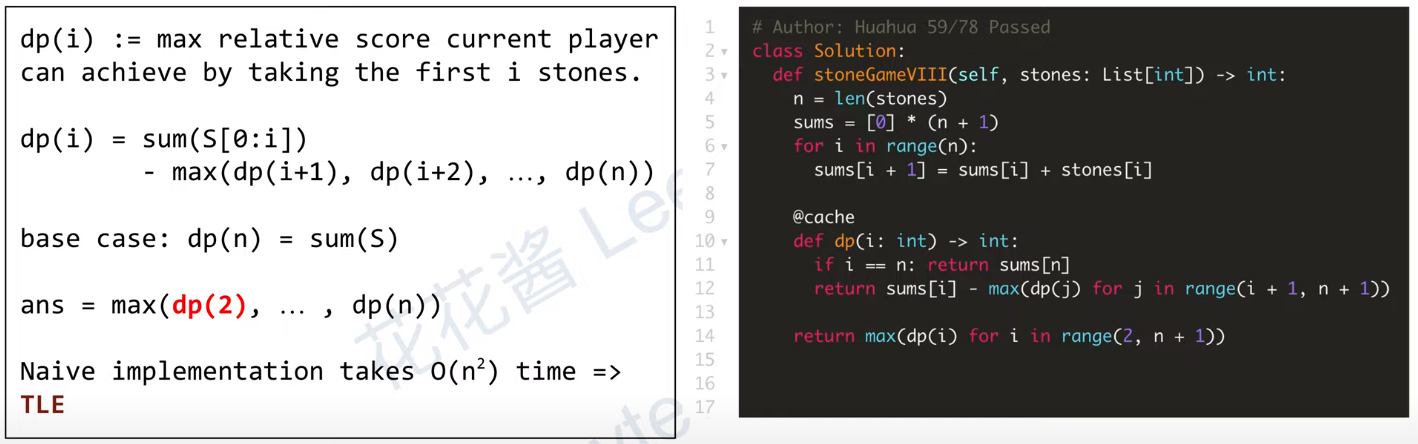
\includegraphics[width=.9\linewidth]{./pic/stone8.png}

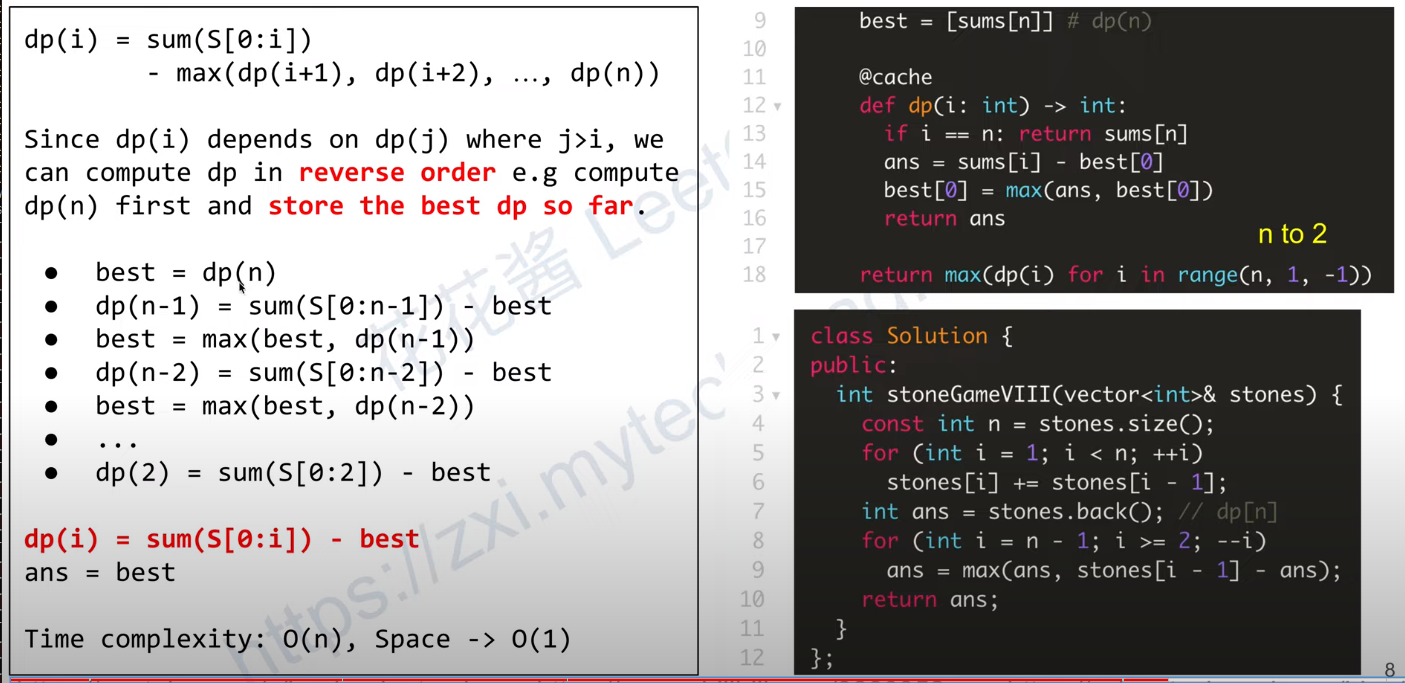
\includegraphics[width=.9\linewidth]{./pic/stone82.png}


\begin{minted}[fontsize=\scriptsize,linenos=false]{csharp}
// 使用 dp(i) 表示还剩下 [i, n) 要选择的情况下,Alice 所能得到的最大分数差。
//     对于某个玩家来说,其对应决策可以分为两种:
//     选取当前数及之前的所有数(等价于 pres[pos],其中 pos 为上个玩家选完后的下个位置),那么 dp[i] = pres[i] - dp[i+1]。
//     这是因为 bob 也会最大化发挥。
//     不选择当前数(可能选下一个,下下一个。。。 etc),那么 dp[i] = dp[i + 1]
public int stoneGameVIII(int[] stones) {
    int n = stones.length;
    int [] dp = new int [n];
    Arrays.fill(dp, Integer.MIN_VALUE);
    int [] pre = new int [n+1];
    for (int i = 1; i <= n; i++)
        pre[i] = pre[i-1] + stones[i-1];
    dp[n-1] = pre[n];
    for (int i = n-2; i >= 0; i--) 
        dp[i] = Math.max(dp[i+1], pre[i+1]-dp[i+1]);
    return dp[1];
}
\end{minted}
\begin{itemize}
\item 更精简的代码如下
\end{itemize}
\begin{minted}[fontsize=\scriptsize,linenos=false]{csharp}
public int stoneGameVIII(int[] stones) {
    int n = stones.length;
    for (int i = 1; i < n; i++) 
        stones[i] += stones[i-1]; // 原位求前缀和
    int ans = stones[n-1];
    for (int i = n-1; i >= 2; i--) 
        ans = Math.max(ans, stones[i-1] - ans); // 一遍反向遍历求最优解
    return ans;
}
\end{minted}
\end{enumerate}

\subsection{464. Can I Win 这个题:为什么顺序无关了?}
\label{sec-1-1-5}
In the "100 game" two players take turns adding, to a running total, any integer from 1 to 10. The player who first causes the running total to reach or exceed 100 wins.
What if we change the game so that players cannot re-use integers?
For example, two players might take turns drawing from a common pool of numbers from 1 to 15 without replacement until they reach a total >= 100.
Given two integers maxChoosableInteger and desiredTotal, return true if the first player to move can force a win, otherwise, return false. Assume both players play optimally.
\begin{minted}[fontsize=\scriptsize,linenos=false]{csharp}
// state是前走的人走完之后的局面,sum是当前数字总和,返回的是当前走的人是否能赢
private boolean dfs(int max, int target, int state, int val) {
    if (dp[state] != -1) return dp[state] > 0;
    if (val >= target) { // 如果对方取数的时候总和达到target了,则当前走的人输了,做记忆并返回false
        dp[state] = 0;
        return false;
    }
    for (int i = 1; i <= max; i++) {  // 枚举当前人取哪个数
        if ((state >> i-1 & 1) == 0 && !dfs(max, target, state | (1 << i-1), val + i)) {
            dp[state] = 1;
            return true;
        }
    }
    dp[state] = 0;
    return false;
}
int [] dp;
public boolean canIWin(int maxChoosableInteger, int desiredTotal) {
    if (desiredTotal <= maxChoosableInteger) return true;
    if (desiredTotal > (maxChoosableInteger + 1)*maxChoosableInteger / 2) return false;
    dp = new int[1 << maxChoosableInteger]; // 时空复杂度O ( 2 m ) O(2^m)O(2 
    Arrays.fill(dp, -1);
    return dfs(maxChoosableInteger, desiredTotal, 0, 0);
}
\end{minted}
\begin{itemize}
\item 另外这第二次又看见的解法
\end{itemize}
\begin{minted}[fontsize=\scriptsize,linenos=false]{csharp}
public boolean canIWin(int maxChoosableInteger, int desiredTotal) { // 这个师与其它类假题相比,为什么顺序无关?
    if (desiredTotal == 0) return true; // 如果1到最大能选的值所有和都不能满足目标值,那么肯定失败
    if ((maxChoosableInteger+1) * maxChoosableInteger / 2 < desiredTotal) return false;
    char [] state = new char [maxChoosableInteger];
    for (int i = 0; i < maxChoosableInteger; i++) state[i] = '0';
    return dfs(desiredTotal, state, new HashMap<>());
}
private boolean dfs(int sum, char [] st, Map<String, Boolean> map) {
    String key = new String(st);
    if (map.containsKey(key)) return map.get(key);
    for (int i = 0; i < st.length; i++) {
        if (st[i] != '0') continue;
        st[i] = '1';
        if (sum <= i+1 || !dfs(sum - (i+1), st, map)) {
            map.put(key, true);
            st[i] = '0';
            return true;
        }
        st[i] = '0';
    }
    map.put(key, false);
    return false;
}
\end{minted}
\begin{itemize}
\item // 下面这个效率更高
\end{itemize}
\begin{minted}[fontsize=\scriptsize,linenos=false]{csharp}
public boolean canIWin(int maxChoosableInteger, int desiredTotal) { 
    if (desiredTotal <= 0) return true;
    int sum = (maxChoosableInteger + 1) * maxChoosableInteger / 2;
    if (sum < desiredTotal) return false;
    boolean[] vis = new boolean[maxChoosableInteger+1];
    return helper(desiredTotal, vis);
}
Map<Integer, Boolean> map = new HashMap<>();
public boolean helper(int desiredTotal, boolean[] vis) {
    if (desiredTotal <= 0) return false;
    int symbol = format(vis);
    if (map.containsKey(symbol)) return map.get(symbol);
    for (int i = 1 ; i < vis.length ; i++) {
        if (!vis[i]) {
            vis[i] = true;
            if (!helper(desiredTotal-i, vis)) {
                vis[i] = false; // 这里不回复状态会影响其它结果
                map.put(symbol, true);
                return true;
            }
            vis[i] = false;
        }
    }
    map.put(symbol, false);
    return false;
}
public int format(boolean[] vis) {
    int symbol = 0;
    for (boolean select : vis) {
        symbol <<= 1;
        if (select) symbol |= 1;
    }
    return symbol;
}
\end{minted}

\subsection{494. Target Sum - Medium}
\label{sec-1-1-6}
You are given an integer array nums and an integer target.

You want to build an expression out of nums by adding one of the symbols '+' and '-' before each integer in nums and then concatenate all the integers.

For example, if nums = [2, 1], you can add a '+' before 2 and a '-' before 1 and concatenate them to build the expression "+2-1".
Return the number of different expressions that you can build, which evaluates to target.
\begin{itemize}
\item 该题是一道非常经典的题目,在面试中很可能会考到。该题有多种解法。
\item 第一种解法:DFS,brute force。我们对nums数组中的每个数字,都尝试在其前面添加正号和负号,最后暴力求解,统计数组中各数字组合值为target的情况。(该理解是错误的,我们可以使用带备忘录机制的自顶向下的DP方法,代码见下)
\end{itemize}
\begin{enumerate}
\item 回溯 O(2\^{}N)
\label{sec-1-1-6-1}
\begin{minted}[fontsize=\scriptsize,linenos=false]{csharp}
private int getAllSums(int [] a, int target, int idx, int sum, int cnt) { // (2^20) 可否一试呢?理论上是可以过的
    if (idx == a.length) {                                                // n < 17 比较好 这个2^N的复朵度,真要命呀。。。。。。
        if (sum == target) cnt++;
        return cnt; // 有return int代码更简洁,但是全局变量cnt效率更高
    }
    // for (int i = idx; i < a.length; i++) { // 为什么要画蝇添足,加个多余的for loop呢? 
        // getAllSums(a, target, idx+1, sum + a[idx]);
        // getAllSums(a, target, idx+1, sum - a[idx]);
    // }
    return getAllSums(a, target, idx+1, sum + a[idx], cnt)
        + getAllSums(a, target, idx+1, sum - a[idx], cnt);
}
public int findTargetSumWays(int[] a, int target) { 
    int n = a.length;
    return getAllSums(a, target, 0, 0, 0);
}
\end{minted}
\item 解题思路与分析: dfs记忆化搜索
\label{sec-1-1-6-2}
\begin{minted}[fontsize=\scriptsize,linenos=false]{csharp}
private int dfs(int [] a, int target, int idx, int sum) {
    String key = idx + "_" + sum;
    if (dp.containsKey(key)) return dp.get(key);
    if (idx == n) {
        if (sum == target) return 1;
        else return 0;
    }
    int add = dfs(a, target, idx+1, sum + a[idx]);
    int sub = dfs(a, target, idx+1, sum - a[idx]);
    dp.put(key, add+sub);
    return add + sub;
}
Map<String, Integer> dp = new HashMap<>();
int n;
public int findTargetSumWays(int[] a, int target) {
    n = a.length;
    return dfs(a, target, 0, 0);
}
\end{minted}
\begin{itemize}
\item 上面的方法比较慢,下面这个效率更好一点儿
\end{itemize}
\begin{minted}[fontsize=\scriptsize,linenos=false]{csharp}
private int dfs(int [] a, int sum, int idx) {
    if (idx == a.length) {
        if (sum == 0) return 1;
        else return 0;
    }
    Map<Integer, Integer> tmp = dp.get(idx);
    if (tmp != null) {
        if (tmp.containsKey(sum))
            return tmp.get(sum);
    } else {
        tmp = new HashMap<>();
        dp.put(idx, tmp);
    }
    int cnt = dfs(a, sum - a[idx], idx+1) + dfs(a, sum + a[idx], idx+1);
    tmp.put(sum, cnt);
    return cnt;
}
Map<Integer, Map<Integer, Integer>> dp = new HashMap<>();
public int findTargetSumWays(int[] nums, int target) {
    return dfs(nums, target, 0);
}
\end{minted}
\item DP
\label{sec-1-1-6-3}
\begin{minted}[fontsize=\scriptsize,linenos=false]{csharp}
// sum[p] + sum[n] = sum[nums];
// sum[p] - sum[n] = S;
// 2sum[p] = sum[nums] + S
// sum[p] = (sum[nums] +S) / 2
public int findTargetSumWays(int [] a, int S) {
    int sum = Arrays.stream(a).sum(), target = (sum + S) / 2; // 根据推导公式,计算出target
    if (S > 0 && sum < S || S < 0 && -sum > S) return 0; // 如果和小于S,说明无法得到解,返回false。(注意S有可能为负)
    if ((sum + S) % 2 != 0) return 0; // 如果计算出的target不是整数,返回false。
    int [] dp = new int [target + 1]; // dp[i]表示在原数组中找出一些数字,并且他们的和为下标i的可能有多少种。
    dp[0] = 1; // 初始化dp[0]为1
    for (Integer v : a) 
        // for (int i = target-v; i >= 0; i--) { // 从0循环到target - n, 注意逆序
        //     if (dp[i] > 0)        // dp[i]大于0说明,存在dp[i]种组合,其和为i的可能性
        //         dp[i+v] += dp[i]; // 既然存在和为i的可能,那么i加上当前数字的和也是存在的
        // }
        for (int i = target; i >= v; i--)  // 从0循环到target - n, 注意逆序
            dp[i] += dp[i-v];              // 两种写法都对
    return dp[target];
}
\end{minted}
\item dp todo
\label{sec-1-1-6-4}
我们使用Vi来表示数组中的前i个数所能求得的和的集合。初始化时
\begin{minted}[fontsize=\scriptsize,linenos=false]{csharp}
V0 = {0}     //表示前0个数的和为0
Vi = {V(i-1) + ai} U {V(i-1) - ai}
\end{minted}

Vn就是nums数组所有数字的组合值之和的集合

根据上面的思路,我们知道数组中数字若全为正号其和为sum,全为负号其和为-sum。若不选数组中任何一个数,则和为0。因此,我们设立一个长度为2*sum+1的数组ways,ways[i]表示我们选择前m个数,其和可能为i的情况数,m = 0,1,\ldots{}nums.length。可参考下图

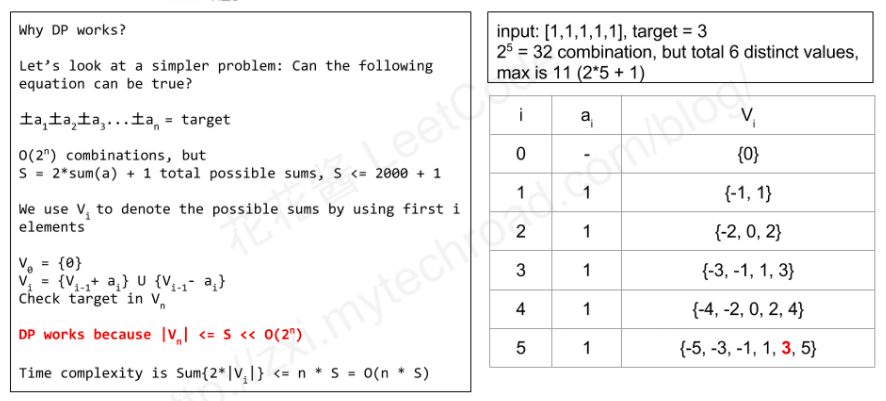
\includegraphics[width=.9\linewidth]{./pic/targetSum.png}

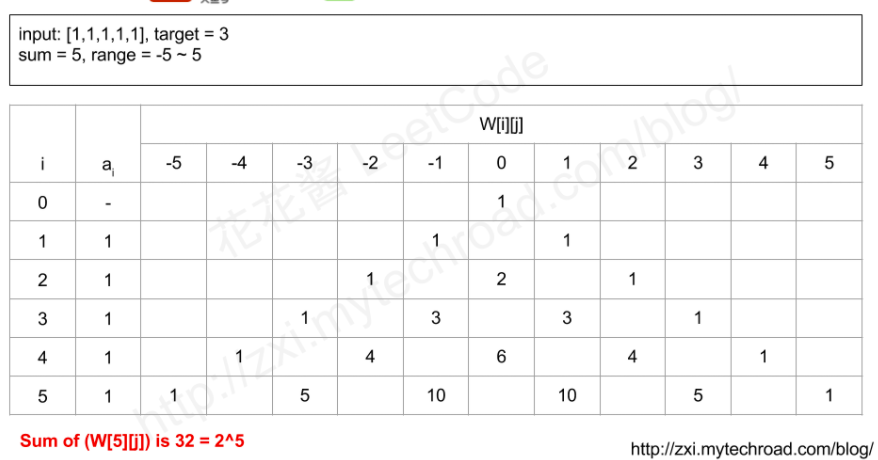
\includegraphics[width=.9\linewidth]{./pic/targetSum2.png}

\url{https://www.cnblogs.com/cnoodle/p/14869498.html}
\url{https://leetcode.com/problems/target-sum/discuss/97334/Java}-(15-ms)-C++-(3-ms)-O(ns)-iterative-DP-solution-using-subset-sum-with-explanation/239290
\url{http://www.noteanddata.com/leetcode-494-Target-Sum-java-solution-note.html}
\url{https://www.i4k.xyz/article/gqk289/54709004}
\url{https://github.com/cherryljr/LeetCode/blob/master/Target\%20Sum.java}
\end{enumerate}

\subsection{647. Palindromic Substrings - Medium}
\label{sec-1-1-7}
Given a string s, return the number of palindromic substrings in it.

A string is a palindrome when it reads the same backward as forward.

A substring is a contiguous sequence of characters within the string.
\begin{minted}[fontsize=\scriptsize,linenos=false]{csharp}
public int countSubstrings(String t) {
    int n = t.length(), ans = 0;
    char [] s = t.toCharArray();
    boolean [][] dp = new boolean [n][n];
    for (int i = n-1; i >= 0; i--) 
        for (int j = i; j < n; j++) {
            dp[i][j] = s[i] == s[j] && (j-i <= 2 || dp[i+1][j-1]);
            if (dp[i][j]) ans++;
        }
    return ans;
}
\end{minted}
\subsection{1444. Number of Ways of Cutting a Pizza - Hard}
\label{sec-1-1-8}
Given a rectangular pizza represented as a rows x cols matrix containing the following characters: 'A' (an apple) and '.' (empty cell) and given the integer k. You have to cut the pizza into k pieces using k-1 cuts. 

For each cut you choose the direction: vertical or horizontal, then you choose a cut position at the cell boundary and cut the pizza into two pieces. If you cut the pizza vertically, give the left part of the pizza to a person. If you cut the pizza horizontally, give the upper part of the pizza to a person. Give the last piece of pizza to the last person.

Return the number of ways of cutting the pizza such that each piece contains at least one apple. Since the answer can be a huge number, return this modulo 10\^{}9 + 7.
\begin{enumerate}
\item 解题思路与分析: 自底向上
\label{sec-1-1-8-1}

常规的矩阵DP做法,这里还需要通过前缀和的思想来快速获取指定范围矩阵的苹果数量。

首先是建立状态表示数组,通过一个三维数组,分别代表矩阵左上角顶点xy坐标和需要分配的人数,数组值表示分该状态下的配方案数;

然后是进行状态转移,从右下角开始枚举所有以该点为状态中左上角的状态,再从低到高枚举需要分配的人数,接着进行切的操作,可以横着切和竖着切,分别枚举所有可能的切除的长度,当前状态的方案数需要从切除后剩下的矩阵状态中进行转移累加。

最后返回以原矩阵左上角为顶点的,分配人数为k的方案数即可。

这里为什么需要将状态表示中的xy设定为矩阵的左上角,还有为什么苹果数的前缀和也是求的右下角的前缀和呢?

因为题意中的切除操作后,要将上半部分或者左半部分给分掉,所以只有右下部分是剩余状态的,我们需要从切除之前的状态获取剩余状态。

\begin{minted}[fontsize=\scriptsize,linenos=false]{csharp}
public int ways(String[] pizza, int p) {
    int mod = (int)1e9 + 7;
    int m = pizza.length, n = pizza[0].length();
    int [][] cnt = new int [m+1][n+1]; // 苹果数的前缀和,用于快速获得在指定矩阵范围内的苹果数量,两个维度也分别是左上角的x、y
    for (int i = m-1; i >= 0; i--) 
        for (int j = n-1; j >= 0; j--) 
            cnt[i][j] = cnt[i+1][j] + cnt[i][j+1] - cnt[i+1][j+1] + (pizza[i].charAt(j) == 'A' ? 1 : 0);
    int [][][] dp = new int [m+1][n+1][p+1]; // 状态数组,三个维度分别表示以x、y为左上角的矩阵中,分给k个人,元素值表示方案数
    for (int i = m-1; i >= 0; i--)       // 遍历矩阵,获取指定左上角矩阵中范围内的苹果数量
        for (int j = n-1; j >= 0; j--) { // 从右下角开始,向左上角开始枚举所有状态
            if (cnt[i][j] > 0) dp[i][j][1] = 1; // 如果这个范围矩阵内存在苹果,那么这个矩阵肯定可以分给1个人,且方案数为1
            for (int k = 2; k <= p; k++) {      // 枚举所有人数状态下的方案,前面已经判断了人数为1的状态,所以这里只需要从2开始枚举
                for (int x = m-1-i; x >= 0; x--)     // 横着切,枚举所有切法
                    if (cnt[i][j] - cnt[i+x][j] > 0) // 如果当前切掉的矩阵内存在苹果,则可以进行状态转移
                        dp[i][j][k] = (dp[i][j][k] + dp[i+x][j][k-1]) % mod;
                for (int y = n-1-j; y >= 0; y--)     // 竖着切
                    if (cnt[i][j] - cnt[i][j+y] > 0)
                        dp[i][j][k] = (dp[i][j][k] + dp[i][j+y][k-1]) % mod;
            }
        }
    return (int)dp[0][0][p];
}
\end{minted}
\item 解题思路与分析: 自顶向下
\label{sec-1-1-8-2}

先用dp方法求出以(i,j)位置为右下角,左上角为(0,0)的区域的苹果数量

建立3维数组,dp[i][j][k]表示切完k次后,剩余蛋糕左上角 在i, j位置时的方案数

初始化,dp\footnote{DEFINITION NOT FOUND.}\textsuperscript{,}\,\footnotemark[1]{}\textsuperscript{,}\,\footnotemark[1]{} = 1

样本维度为切的次数 k

状态维度,这次切之前的状态(蛋糕左上角位置 i, j)

状态转移,这次切完后蛋糕左上角位置(横向切,ni,j;竖向切,i, nj,切的次数 +1)

转移条件:切出去的蛋糕当中有苹果(用上面求得的苹果数量,dp公式求得)

最后求结果总和:最后的一块蛋糕中有苹果,sum += dp[i][j][k-1]
\begin{minted}[fontsize=\scriptsize,linenos=false]{csharp}
public int ways(String[] pizza, int p) { // 自顶向下: 与自底向上相比
    int mod = (int)1e9 + 7;
    int m = pizza.length, n = pizza[0].length();
    int [][] cnt = new int [m+1][n+1];  // 苹果数的前缀和,用于快速获得在指定矩阵范围内的苹果数量,两个维度也分别是左上角的x、y
    for (int i = 1; i <= m; i++) 
        for (int j = 1; j <= n; j++) 
            cnt[i][j] = cnt[i-1][j] + cnt[i][j-1] - cnt[i-1][j-1] + (pizza[i-1].charAt(j-1) == 'A' ? 1 : 0);
    int [][][] dp = new int [m+1][n+1][p]; // dp[i][j][k]表示切完k次后,剩余蛋糕左上角 在i,j位置时的方案数
    dp[1][1][0] = 1; // 初始值是为了程序的运行,
    for (int k = 1; k < p; k++) 
        for (int i = 1; i <= m; i++) 
            for (int j = 1; j <= n; j++) {
                System.out.println("(dp[i][j][k-1] == 0) : " + (dp[i][j][k-1] == 0) );
                if (dp[i][j][k-1] == 0) continue; // 上一次cut完后,剩余蛋糕左上角在i,j
                for (int x = i+1; x <= m; x++)   // 横向切,切完后的剩余左上角为 x, j
                    if (cnt[x-1][n] - cnt[i-1][n] - cnt[x-1][j-1] + cnt[i-1][j-1] > 0)
                        dp[x][j][k] = (dp[x][j][k] + dp[i][j][k-1]) % mod;
                for (int y = j+1; y <= n; y++)  // 竖向切
                    if (cnt[m][y-1] - cnt[m][j-1] - cnt[i-1][y-1] + cnt[i-1][j-1] > 0)
                        dp[i][y][k] = (dp[i][y][k] + dp[i][j][k-1]) % mod;
            }
    long ans = 0;
    for (int i = 1; i <= m; i++) 
        for (int j = 1; j <= n; j++) 
            if (cnt[m][n] - cnt[i-1][n] - cnt[m][j-1] + cnt[i-1][j-1] > 0) // 先前并没有确认切的结果有效,即最后剩下的那块是否有苹果
                ans = (ans + dp[i][j][p-1]) % mod;                         // 统计结果的时候,要先确保有效
    return (int)ans;
}
\end{minted}
\end{enumerate}


\section{字符串、数组等双序列}
\label{sec-1-2}

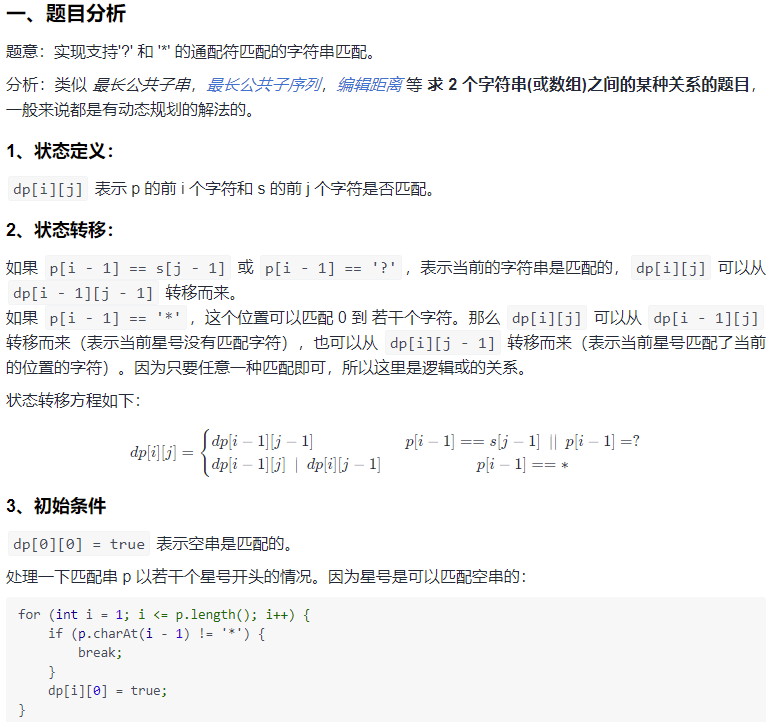
\includegraphics[width=.9\linewidth]{./pic/doubSeq.png}

\subsection{题目拓展}
\label{sec-1-2-1}
\begin{enumerate}
\item 718. 最长重复子数组 (类似题目,只是由字符串变为数组)
\label{sec-1-2-1-1}
\item 72. 编辑距离
\label{sec-1-2-1-2}
\item 1143. 最长公共子序列
\label{sec-1-2-1-3}
\item 10. 正则表达式匹配
\label{sec-1-2-1-4}
\item 583. 两个字符串的删除操作
\label{sec-1-2-1-5}
\item 727. 最小窗口子序列
\label{sec-1-2-1-6}

你会发现这些都是 求 2 个字符串(或数组)之间的某种关系的题目
\end{enumerate}
\subsection{10. Regular Expression Matching - Hard}
\label{sec-1-2-2}
Given an input string s and a pattern p, implement regular expression matching with support for '.' and '*' where:

'.' Matches any single character.​​​​
'*' Matches zero or more of the preceding element.
The matching should cover the entire input string (not partial).
\begin{enumerate}
\item 解题思路与分析
\label{sec-1-2-2-1}

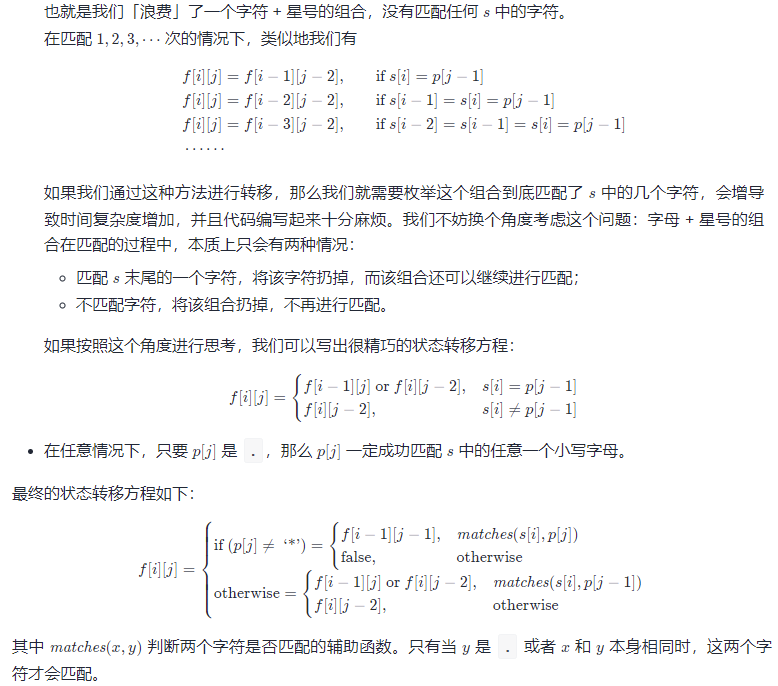
\includegraphics[width=.9\linewidth]{./pic/regMatch.png}

\begin{minted}[fontsize=\scriptsize,linenos=false]{csharp}
public boolean isMatch(String s, String p) {
    int m = s.length();
    int n = p.length();
    boolean[][] f = new boolean[m + 1][n + 1];
    f[0][0] = true;
    for (int i = 0; i <= m; ++i) 
        for (int j = 1; j <= n; ++j) 
            if (p.charAt(j - 1) == '*') {
                f[i][j] = f[i][j - 2];
                if (matches(s, p, i, j - 1)) 
                    f[i][j] = f[i][j] || f[i - 1][j];
            } else {
                if (matches(s, p, i, j)) 
                    f[i][j] = f[i - 1][j - 1];
            }
    return f[m][n];
}
public boolean matches(String s, String p, int i, int j) {
    if (i == 0) return false;
    if (p.charAt(j - 1) == '.') return true;
    return s.charAt(i - 1) == p.charAt(j - 1);
}
\end{minted}
\end{enumerate}
\subsection{115. Distinct Subsequences - Hard}
\label{sec-1-2-3}
Given two strings s and t, return the number of distinct subsequences of s which equals t.

A string's subsequence is a new string formed from the original string by deleting some (can be none) of the characters without disturbing the remaining characters' relative positions. (i.e., "ACE" is a subsequence of "ABCDE" while "AEC" is not).

It is guaranteed the answer fits on a 32-bit signed integer.
\begin{enumerate}
\item 解题思路与分析
\label{sec-1-2-3-1}
这道题不是求两个字符串是匹配,而是判断S有多少种方式可以得到T。但其实还是动态规划,我们一个定义二维数组dp,dp[i][j]为字符串s(0,i)变换到t(0,j)的变换方法的个数。

如果S[i]==T[j],那么dp[i][j] = dp[i-1][j-1] + dp[i-1][j]

意思是:如果当前S[i]==T[j],那么当前这个字符即可以保留也可以抛弃,所以变换方法等于保留这个字符的变换方法加上不用这个字符的变换方法, 

dp[i-1][j-1]为保留这个字符时的变换方法个数,dp[i-1][j]表示抛弃这个字符时的变换方法个数。

如果S[i]!=T[i],那么dp[i][j] = dp[i-1][j],意思是如果当前字符不等,那么就只能抛弃当前这个字符。

\begin{minted}[fontsize=\scriptsize,linenos=false]{csharp}
public int numDistinct(String ss, String tt) {
    int m = ss.length(), n = tt.length();
    char [] s = ("#"+ss).toCharArray();
    char [] t = ("#"+tt).toCharArray();
    int [][] dp = new int [m+1][n+1];
    dp[0][0] = 1;
    for (int j = 1; j <= n; j++) // 注意这两行初始状态的设置
        dp[0][j] = 0;
    for (int i = 1; i <= m; i++) 
        dp[i][0] = 1;
    for (int i = 1; i <= m; i++) 
        for (int j = 1; j <= n; j++) 
            if (s[i] == t[j])
                dp[i][j] = dp[i-1][j-1] + dp[i-1][j];
            else dp[i][j] = dp[i-1][j];
    return dp[m][n];
}
\end{minted}
\end{enumerate}

\subsection{将一个数组分为两个部分,分别求和S1与S2,使得|S1-S2|最小}
\label{sec-1-2-4}

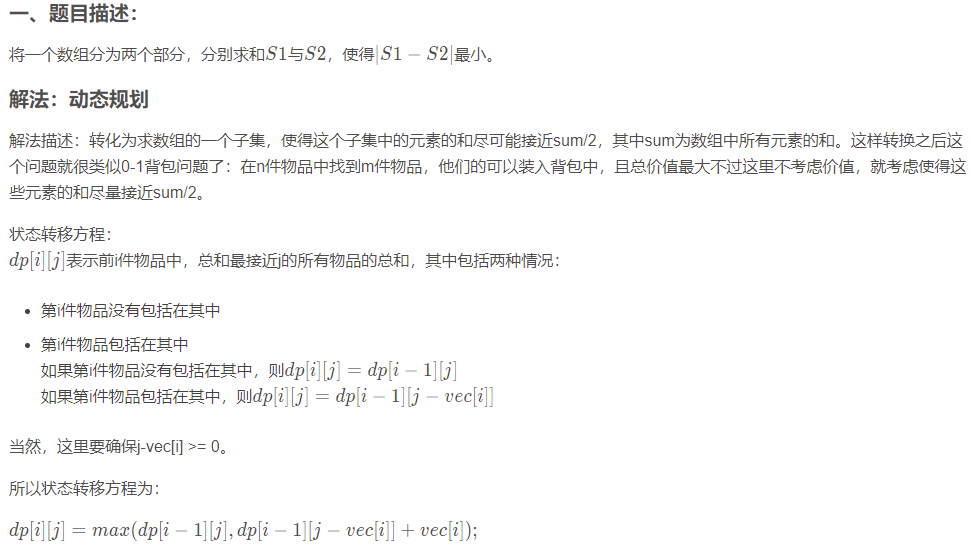
\includegraphics[width=.9\linewidth]{./pic/dpArray.png}

\begin{minted}[fontsize=\scriptsize,linenos=false]{csharp}
public static int getMaxDiff(int[] array) {
    int sum = Arrays.stream(array).sum();
    int length = array.length;
    int [][] f = new int[length+1][sum/2+1];
    for (int i = 0; i < length; i++) 
        for (int j = 1; j <  = sum/2; j++) {
            f[i+1][j]  =  f[i][j];
            if (array[i] <= j && f[i][j-array[i]] + array[i] > f[i][j]) 
                f[i+1][j] = f[i][j-array[i]] + array[i];
        }
    return sum-2*f[length][sum/2];
}
\end{minted}
\subsection{给定一个序列,不保证有序,求这个序列的最长等差序列的长度。}
\label{sec-1-2-5}

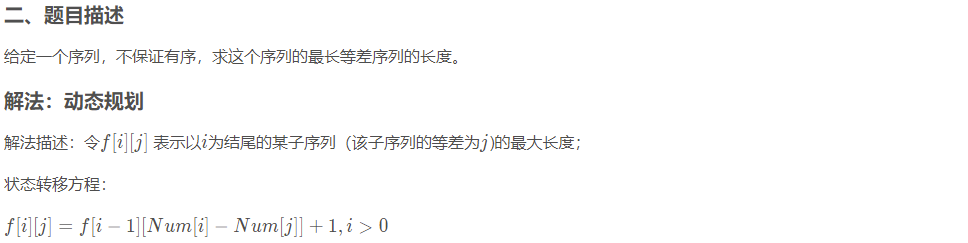
\includegraphics[width=.9\linewidth]{./pic/dpArray2.png}

\begin{minted}[fontsize=\scriptsize,linenos=false]{csharp}
private static int lengthOfLongest(int[] set){
    Arrays.sort(set);
    int n = set.length;
    if (n <= 2) return n;
    int llap = 2;
    int[][] dp = new int[n][n];
    for (int i=0; i<n; i++) dp[i][n-1] = 2;
    for (int j=n-2; j>=1; j--) {
        int i=j-1, k=j+1;
        while (i>=0 && k<=n-1) {
            if (set[i] + set[k] < 2 * set[j])
                k++;
            else if (set[i] + set[k] > 2 * set[j]) {
                dp[i][j] = 2;
                i--;
            } else {
                dp[i][j] = dp[j][k] + 1;
                llap = Math.max(llap, dp[i][j]);
                i--;
                k++;
            }
        }
        while (i >= 0) {
            dp[i][j] = 2;
            i--;
        }
    }
    return llap;
}
\end{minted}
\subsection{求一个序列的最长子序列,使得最多修改一个数字使得这个子序列的为严格递增序列}
\label{sec-1-2-6}

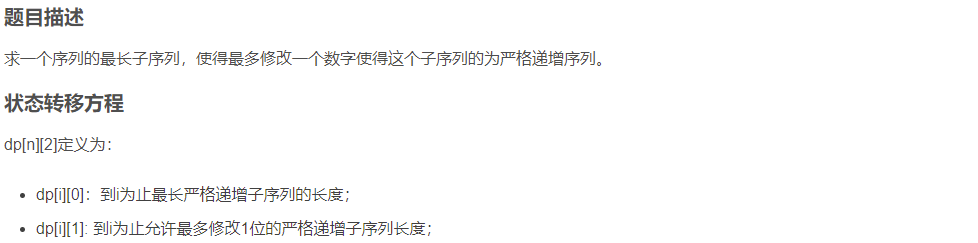
\includegraphics[width=.9\linewidth]{./pic/dpArray3.png}
\begin{minted}[fontsize=\scriptsize,linenos=false]{csharp}
private static int getMaxLength(int[] arr){
    if (arr.length <= 2) return arr.length;
    int[][] dp = new int[arr.length][2];
    dp[0][0] = 1;
    dp[0][1] = 1;
    for (int i = 1; i < arr.length; i++) {
        dp[i][0] = dp[i-1][0]+1;
        if (arr[i] <= arr[i-1])
            dp[i][0]--;
        if (dp[i-1][0] == dp[i-1][1] && arr[i] <= arr[i-1]) {// 说明前面还没有改的
            dp[i][1] = dp[i][0] + 1;
            arr[i] = arr[i-1]+1;
        } else {//说明前面已经改动或者arr[i] <= arr[i-1]
            if (arr[i] > arr[i-1]) {
                //判断前面是否已经改动
                dp[i][1] = dp[i-1][1]+1;
                if (dp[i-1][0] != dp[i-1][1]) 
                    dp[i][1]--;
            } else
                dp[i][1] = dp[i-1][1];
        }
    }
    return dp[arr.length-1][1];
}
\end{minted}

\subsection{801. Minimum Swaps To Make Sequences Increasing - Hard}
\label{sec-1-2-7}
You are given two integer arrays of the same length nums1 and nums2. In one operation, you are allowed to swap nums1[i] with nums2[i].

For example, if nums1 = [1,2,3,8], and nums2 = [5,6,7,4], you can swap the element at i = 3 to obtain nums1 = [1,2,3,4] and nums2 = [5,6,7,8].
Return the minimum number of needed operations to make nums1 and nums2 strictly increasing. The test cases are generated so that the given input always makes it possible.

An array arr is strictly increasing if and only if arr\footnotemark[1]{} < arr\footnote{DEFINITION NOT FOUND.} < arr\footnote{DEFINITION NOT FOUND.} < \ldots{} < arr[arr.length - 1].
\begin{enumerate}
\item 解题思路与分析
\label{sec-1-2-7-1}
\begin{minted}[fontsize=\scriptsize,linenos=false]{csharp}
// 设 dp[0][i] 表示不交换 A[i] 和 B[i] 在下标 i 的交换次数
// 设 dp[1][i] 表示交换 A[i] 和 B[i] 在下标 i 的交换次数
// 可以看到交换与否只取决与前一个状态, 可以将空间复杂度压缩到 O(1)
//     时间复杂度为 O(n), 空间复杂度为 O(1)
public int minSwap(int[] a, int[] b) {
    int n = a.length;
    int [][] dp = new int [n][2]; // 0: 不换, 1: 换
    for (int i = 0; i < n; i++) 
        Arrays.fill(dp[i], Integer.MAX_VALUE);
    dp[0][0] = 0;
    dp[0][1] = 1;
    for (int i = 1; i < n; i++) {
        if (a[i] > a[i-1] && b[i] > b[i-1]) {
            dp[i][0] = Math.min(dp[i][0], dp[i-1][0]);     // 不换,取一个较小值
            dp[i][1] = Math.min(dp[i][1], dp[i-1][1] + 1); // 换就两个都换
        }
        if (a[i] > b[i-1] && b[i] > a[i-1]) {
            dp[i][0] = Math.min(dp[i][0], dp[i-1][1]); 
            dp[i][1] = Math.min(dp[i][1], dp[i-1][0] + 1);
        }
    }
    return Math.min(dp[n-1][0], dp[n-1][1]);
}
\end{minted}
\end{enumerate}

\subsection{1639. Number of Ways to Form a Target String Given a Dictionary - Hard}
\label{sec-1-2-8}
You are given a list of strings of the same length words and a string target.

Your task is to form target using the given words under the following rules:

target should be formed from left to right.
To form the ith character (0-indexed) of target, you can choose the kth character of the jth string in words if target[i] = words[j][k].
Once you use the kth character of the jth string of words, you can no longer use the xth character of any string in words where x <= k. In other words, all characters to the left of or at index k become unusuable for every string.
Repeat the process until you form the string target.
Notice that you can use multiple characters from the same string in words provided the conditions above are met.

Return the number of ways to form target from words. Since the answer may be too large, return it modulo 109 + 7.
\begin{enumerate}
\item 解题思路与分析: dp
\label{sec-1-2-8-1}
\begin{minted}[fontsize=\scriptsize,linenos=false]{csharp}
   思路:
   dp[i][j]  表示:words字符串列表的前 j 列来构造目标字符串target的前 i 个字符;
   cnt[i][j] 表示:words字符串列表的第 i 列 一共有多少 字符 j ;
   那dp公式就很好推出来了:
   1.第i个字符不使用第j列时,即通过前 j - 1 列得到
     dp[i][j] = dp[i][j-1];
   2.第i个字符使用第j列时
   *   dp[i][j] = dp[i-1][j-1] * cnt[j][第i个字符];
   ==>>dp[i][j] = dp[i][j-1] + dp[i-1][j-1] * cnt[j][第i个字符]
\end{minted}
\begin{minted}[fontsize=\scriptsize,linenos=false]{csharp}
static final int mod = (int)1e9 + 7;
public int numWays(String[] words, String target) {
    int m = target.length(), n = words[0].length();
    char [] s = target.toCharArray();
    int [][] cnt = new int [n][26];
    for (String w : words) 
        for (int j = 0; j < n; j++) 
            cnt[j][w.charAt(j)-'a']++;
    // long [][] dp = new long [m][n];
    // dp[0][0] = cnt[0][s[0]-'a'];
    // for (int i = 1; i < n; i++) // 初始化: 由前i列来构成target第一个字符的方案数
    //     dp[0][i] = (dp[0][i] + dp[0][i-1] + cnt[i][s[0]-'a']) % mod;
    // for (int i = 1; i < m; i++) 
    //     for (int j = i; j < n; j++) 
    //         dp[i][j] = (dp[i][j-1] + dp[i-1][j-1] * cnt[j][s[i]-'a']) % mod;
    // return (int)dp[m-1][n-1];
    long [][] dp = new long [m+1][n+1];
    Arrays.fill(dp[0], 1l);
    // dp[0] = LongStream.range(0, n+1).map(e->1).toArray(); // 上下两行,效果差不多,filling first row of array with 1
    for (int i = 1; i <= m; i++)
        for (int j = i; j <= n + i - m; j++) 
            dp[i][j] = (dp[i][j-1] + dp[i-1][j-1] * cnt[j-1][s[i-1]-'a'] % mod) % mod;
    return (int)dp[m][n];
}
\end{minted}
\begin{itemize}
\item dp降维,压缩空间
\end{itemize}
\begin{minted}[fontsize=\scriptsize,linenos=false]{csharp}
static final int mod = (int)1e9 + 7;
public int numWays(String[] words, String target) { // dp降维,压缩空间,但二维dp仍然是思路最为清晰好理解的
    int m = target.length(), n = words[0].length();
    char [] s = target.toCharArray();
    long [] dp = new long [m];
    for (int i = 0; i < n; i++) {  // 遍历字符数组的各列
        int [] cnt = new int [26]; // 当前-列-所有字符的出现次数
        for (String w : words) 
            cnt[w.charAt(i)-'a']++;
        for (int j = Math.min(i, m-1); j >= 0; j--) // 记住: 降维就容易产生赃数据,需要倒序遍历
            dp[j] = (dp[j] + (j > 0 ? dp[j-1] : 1) * cnt[s[j]-'a']) % mod;
    }
    return (int)dp[m-1];
}
\end{minted}
\end{enumerate}

\section{区间型DP}
\label{sec-1-3}
\begin{itemize}
\item \url{https://leetcode-cn.com/problems/minimum-cost-to-merge-stones/solution/yi-dong-you-yi-dao-nan-yi-bu-bu-shuo-ming-si-lu-he/}
\end{itemize}

区间dp问题,旨在通过动态规划去求一个区间的最优解,通过将大区间划分为很多个小区间,再由小区间的解来组合出大区间的解,这体现了分治的思想。

\begin{itemize}
\item 区间动态规划三部曲
\begin{itemize}
\item 定义状态:dp[i, j]为区间[i, j]的最优解
\item 定义状态转移方程:最常见的写法为:dp[i,j] = max/min\{dp[i,j], dp[i, k] + dp[k+1, j] + cost\}。选取[i, j]之间的一个分界点k,分别计算[i, k]和[k+1, j]的最优解,从而组合出[i, j]的最优解。
\item 初始化:dp[i][i] = 常数。区间长度为1时的最优解应当是已知的。
\end{itemize}
\end{itemize}

假设要求的区间最优解为dp[1, n],区间dp问题有两种编码方法:

\begin{itemize}
\item 第一种:
\end{itemize}
\begin{minted}[fontsize=\scriptsize,linenos=false]{csharp}
for (int i = n; i >= 1; --i) 
    for (int j = i + 1; j <= n; ++j) 
        for (int k = i; k < j; ++k) 
            dp[i,j] = max/min(dp[i,j], dp[i,k] + dp[k+1, j] + cost)
\end{minted}

这种写法就是常规的dp写法,枚举i为子区间左边界,枚举j为子区间有边界,枚举k为分界点。要注意由于要求的是dp[1,n],所以i必须从大往小遍历,j必须从小往大遍历。这样在状态转移方程中利用的就是已求解的dp状态。
\begin{itemize}
\item 第二种:
\end{itemize}
\begin{minted}[fontsize=\scriptsize,linenos=false]{csharp}
for (int len = 2; len <= n; ++len) 
    for (int i = 1; i + len - 1  <= n; ++i) {
        int j = i + len - 1;
        for (int k = i; k < j; ++k) 
            dp[i,j] = max/min(dp[i,j], dp[i,k] + dp[k+1, j] + cost;
    }
\end{minted}

这种写法最常见,枚举len为区间长度,枚举i为区间左端点,由此可以计算出区间右端点j,枚举k为分界点。区间长度从2到n,跟上一种写法相同。这种写法的正确性可能不如上一种那么直观,它从小到大枚举出所有区间,在求解大区间时,状态转移方程中利用的状态都是小区间的状态,必定在它之前被求解,所以也是正确的。

\subsection{1039. Minimum Score Triangulation of Polygon - Medium}
\label{sec-1-3-1}
You have a convex n-sided polygon where each vertex has an integer value. You are given an integer array values where values[i] is the value of the ith vertex (i.e., clockwise order).

You will triangulate the polygon into n - 2 triangles. For each triangle, the value of that triangle is the product of the values of its vertices, and the total score of the triangulation is the sum of these values over all n - 2 triangles in the triangulation.

Return the smallest possible total score that you can achieve with some triangulation of the polygon.

\begin{minted}[fontsize=\scriptsize,linenos=false]{csharp}
// 动态规划,递归可以使逻辑简单(本质还是动态规划)将多边形起始位置设为start,end, 用一个数组dp来记录任意起始位置的score
// 为了计算dp[start][end], 我们用一个index k在start到end之间遍历
// dp[start][end] = min(dp[start][k] + dp[k][end] + A[start]* A[k] * A[end])结果为dp[0][n - 1]注意:相邻的dp[i][i + 1] = 0, 因为两条边无法组成三角形
private int dfs(int [] a, int i, int j) {
    if (j - i < 2) return 0; // 最开始终止条件没有写对
    if (dp[i][j] > 0) return dp[i][j];
    int ans = Integer.MAX_VALUE;
    for (int k = i+1; k < j; k++) 
        ans = Math.min(ans, a[i]*a[k]*a[j] + dfs(a, i, k) + dfs(a, k, j));
    return dp[i][j] = ans;
}
int [][] dp;
int n;
public int minScoreTriangulation(int[] a) {
    n = a.length;
    dp = new int [n][n];
    return dfs(a, 0, n-1);
}
\end{minted}

\subsection{2019. The Score of Students Solving Math Expression - Hard 有人说这是区间dp,无感}
\label{sec-1-3-2}
You are given a string s that contains digits 0-9, addition symbols '+', and multiplication symbols '*' only, representing a valid math expression of single digit numbers (e.g., 3+5*2). This expression was given to n elementary school students. The students were instructed to get the answer of the expression by following this order of operations:

Compute multiplication, reading from left to right; Then,
Compute addition, reading from left to right.
You are given an integer array answers of length n, which are the submitted answers of the students in no particular order. You are asked to grade the answers, by following these rules:

If an answer equals the correct answer of the expression, this student will be rewarded 5 points;
Otherwise, if the answer could be interpreted as if the student applied the operators in the wrong order but had correct arithmetic, this student will be rewarded 2 points;
Otherwise, this student will be rewarded 0 points.
Return the sum of the points of the students.
\begin{enumerate}
\item 解题思路与分析
\label{sec-1-3-2-1}
\begin{itemize}
\item 思路是记忆化搜索。先求一下正确答案,然后开始算所有可能得到的错误答案。枚举运算符,然后递归求解两边可能的答案,汇总成当前表达式可能得到的答案。用记忆化的方式避免重复计算。
\item 时间复杂度O(l\_s\^{}3+l\_A)),空间O(l\_s\^{}2)。注意有1000这个限制,上面所说的复杂度的常数是1000\^{}2,是很大的
\end{itemize}

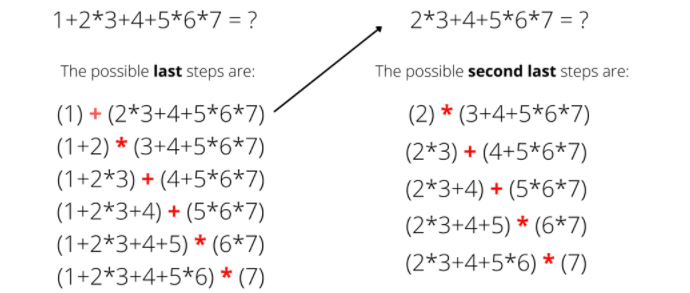
\includegraphics[width=.9\linewidth]{./pic/score.png}

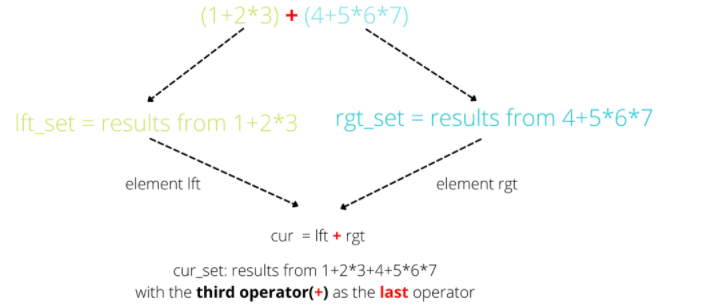
\includegraphics[width=.9\linewidth]{./pic/score2.png}

\begin{minted}[fontsize=\scriptsize,linenos=false]{csharp}
private int compute(String t) {
    ArrayDeque<Integer> st = new ArrayDeque<>();
    char [] s = t.toCharArray();
    for (int i = 0; i < s.length; i++) {
        char c = s[i];
        if (Character.isDigit(c)) 
            if (i > 0 && s[i-1] == '*') 
                st.push(st.pop() * (c-'0'));
            else st.push(c-'0');
    }
    int ans = 0;
    while (!st.isEmpty()) 
        ans += st.pop();
    return ans;
}
Set<Integer> dfs(String t, int l, int r, Set<Integer> [][] f) {
    if (f[l][r] != null) return f[l][r]; // 有记忆则调取记忆
    char [] s = t.toCharArray();
    int n = t.length(), v = 0;
    f[l][r] = new HashSet<>();
    if (l == r) {
        f[l][r].add(s[l] - '0');
        return f[l][r];
    }
    for (int i = l+1; i < r; i++) 
        if (!Character.isDigit(s[i])) { // 递归求解左右两边可能算出的答案
            Set<Integer> left = dfs(t, l, i-1, f);
            Set<Integer> right = dfs(t, i+1, r, f);
            for (Integer va : left) 
                for (Integer vb : right) {
                    if (s[i] == '*') v = va * vb;
                    else v = va + vb;
                    if (v >= 0 && v <= 1000) f[l][r].add(v);
                }
        }
    return f[l][r];
}
public int scoreOfStudents(String s, int [] num) { 
    int m = num.length, res = compute(s), n = s.length(), ans = 0;
    Set<Integer> [][] f = new HashSet[n][n]; // 第一次见,学习一下
    dfs(s, 0, n-1, f);
    Set<Integer> can = f[0][n-1];        // candidates: of wrong answers
    for (Integer v : num) 
        if (v == res) ans += 5;
        else if (can.contains(v)) ans += 2;
    return ans;
}
\end{minted}
\end{enumerate}

\subsection{312. Burst Balloons 区间型动态规划的典型代表}
\label{sec-1-3-3}
You are given n balloons, indexed from 0 to n - 1. Each balloon is painted with a number on it represented by an array nums. You are asked to burst all the balloons.
If you burst the ith balloon, you will get nums[i - 1] * nums[i] * nums[i + 1] coins. If i - 1 or i + 1 goes out of bounds of the array, then treat it as if there is a balloon with a 1 painted on it.
Return the maximum coins you can collect by bursting the balloons wisely.
\begin{minted}[fontsize=\scriptsize,linenos=false]{csharp}
public int maxCoins(int[] nums) {
    int n = nums.length;
    int [][]  dp = new int [n+2][n+2];
    int [] arr = new int [n+2];
    System.arraycopy(nums, 0, arr, 1, n);
    arr[0] = arr[n+1] = 1;  // [0, n+1] ==> [1, n]
    int j = 0;
    for (int len = 1; len <= n; len++) { // [1, n]
        for (int i = 1; i+len-1 <= n; i++) { // [1, n]
            j = i + len - 1;
            for (int k = i; k <= j; k++) 
                dp[i][j] = Math.max(dp[i][j], dp[i][k-1] + dp[k+1][j] + arr[i-1]*arr[k]*arr[j+1]);
        }
    }
    return dp[1][n];
}
// 0    0    0    0    0    0
// 0    3    30   159  167  0
// 0    0    15   135  159  0
// 0    0    0    40   48   0
// 0    0    0    0    40   0
// 0    0    0    0    0    0
private int memorizedSearch(int [] arr, int x, int y) {
    if (dp[x][y] > 0) return dp[x][y];
    // if (x == y) return dp[x][y] = arr[x]; // 没有这些个边际条件
    // if (x == y-1) 
    //     return dp[x][y] = arr[x] * arr[y] + Math.max(arr[x], arr[y]);
    int max = 0;
    for (int i = x; i <= y; i++) {
        max = Math.max(max, memorizedSearch(arr, x, i-1) + memorizedSearch(arr, i+1, y) + arr[x-1]*arr[i]*arr[y+1]);
    }
    return dp[x][y] = max;
}
int [][] dp;
int n;
public int maxCoins(int[] nums) {
    int n = nums.length + 2;
    dp = new int [n][n];
    int [] arr = new int [n];
    System.arraycopy(nums, 0, arr, 1, n-2);
    arr[0] = arr[n-1] = 1;
    return memorizedSearch(arr, 1, n-2);
}
\end{minted}

\subsection{1000. Minimum Cost to Merge Stones - Hard}
\label{sec-1-3-4}
There are n piles of stones arranged in a row. The ith pile has stones[i] stones.
A move consists of merging exactly k consecutive piles into one pile, and the cost of this move is equal to the total number of stones in these k piles.
Return the minimum cost to merge all piles of stones into one pile. If it is impossible, return -1.
\begin{enumerate}
\item 解题思路与分析
\label{sec-1-3-4-1}

看到了论坛上有人定义了三维的 dp 数组,把每次合并的堆数K也当作一维放入到 dp 数组中了,其实博主觉得不是很有必要,因为像这种必须要对 dp 数组进行升维操作的是当题目中有隐藏信息 Hidden Information,而当前定义的 dp 数组无法重现子问题,即无法找到状态转移方程的时候必须要做的,最典型的例子就是之前那道 Remove Boxes,那道题自区间的 dp 值非常依赖于区间左边相同的数字的个数,而这道题每次合并的堆数K并不是很依赖其他小于K的合并的堆数,所以博主感觉没有必要加。

\begin{minted}[fontsize=\scriptsize,linenos=false]{csharp}
public int mergeStones(int[] stones, int k) {
    int n = stones.length;
    if ((n-1) % (k-1) != 0) return -1;
    int [][] dp = new int[n][n];
    int [] pre = new int[n+1];
    for (int i = 1; i <= n; i++) 
        pre[i] = pre[i-1] + stones[i-1];
    int j = 0;
    for (int len = k; len <= n; len++) {
        for (int i = 0; i+len-1 < n; i++) {
            j = i + len -1;
            dp[i][j] = Integer.MAX_VALUE; // have to initialize it here !!!
            for (int x = i; x < j; x += k-1) 
                dp[i][j] = Math.min(dp[i][j], dp[i][x] + dp[x+1][j]);
            if ((j - i) % (k - 1) == 0) // 如果总长度满足合并只剩一个数的条件,则可以再合并一次
                dp[i][j] += pre[j+1] - pre[i];
        }
    }
    return dp[0][n-1];
}
\end{minted}
\item 解题思路与分析: 上述解法的时间复杂度是O(n\^{}3*k).我们可以对它进行优化。
\label{sec-1-3-4-2}
\begin{itemize}
\item \url{https://leetcode.com/problems/minimum-cost-to-merge-stones/discuss/247657/JAVA-Bottom-Up-\%2B-Top-Down-DP-With-Explaination}
\end{itemize}

定义dp[i][j]为尽可能多的合并区间[i, j] 所需的成本,不一定能合并成一堆,但合并完成后剩下的堆数一定小于k,更具体地,剩余的堆数一定是(n - 1) \% (k - 1) + 1。

证明:

已知一次合并会导致堆数减少k-1,假设最多进行了a次合并,则有

remain = n - (k - 1) * a,1 <= remain <= k - 1,

$\Rightarrow$⇒ remain - 1 = n - 1 - (k - 1) * a

$\Rightarrow$⇒ remain - 1 = (n - 1) \% (k - 1)

$\Rightarrow$⇒ remain = (n - 1) \% (k - 1) + 1

证毕。

我们参照解法一来定义状态转移方程,同样将区间[i,j]划分为两部分。

我们保证将左部分合并成1堆,而尽可能多地合并右部分。(左部分需要满足(len - 1) \% (k - 1) == 0)。

右部分剩余堆数满足1 <= remain <= k - 1,如果最后右部分剩余k-1堆(也即(j - i) \% (k - 1) == 0),则还可以继续将这两部分合并成1堆。

因此合并区间[i,j]的成本是合并其左右部分成本之和(对于最优的划分)。如果可以进一步合并的话,则额外的成本是sum(i, j)。

状态转移方程为:dp[i][j] = min(dp[i][p] + dp[p + 1][j]), i <= p < j,如果可以继续合并,dp[i][j] += sum(i, j)。

这样的话枚举的区间长度就必须从k开始了,因为长度在[1,k-1]之间的区间已经无法进行合并了,它们的dp[i][j] == 0。

\begin{minted}[fontsize=\scriptsize,linenos=false]{csharp}
public int mergeStones(int[] s, int k) {
    int n = s.length;
    if ((n - 1) % (k - 1) != 0) return -1;
    int [][] dp = new int [n+1][n+1];
    int [] sum = new int [n+1];
    for (int i = 1; i <= n; i++)  sum[i] = sum[i-1] + s[i-1];
    for (int len = k; len <= n; len++) // 枚举区间长度
        for (int i = 1; i+len <= n+1; i++) { // 枚举区间起点
            int j = i + len - 1;
            dp[i][j] = Integer.MAX_VALUE;
            for (int p = i; p < j; p += k-1) // 枚举分界点
                dp[i][j] = Math.min(dp[i][j], dp[i][p] + dp[p+1][j]);
            if ((j - i) % (k-1) == 0) dp[i][j] += sum[j] - sum[i-1];
        }
    return dp[1][n];
}
\end{minted}
\end{enumerate}

\subsection{546. Remove Boxes - Hard: 带隐含信息,需要第三维参数加入的}
\label{sec-1-3-5}
You are given several boxes with different colors represented by different positive numbers.

You may experience several rounds to remove boxes until there is no box left. Each time you can choose some continuous boxes with the same color (i.e., composed of k boxes, k >= 1), remove them and get k * k points.

Return the maximum points you can get.
\begin{enumerate}
\item 解题思路与分析
\label{sec-1-3-5-1}
\begin{minted}[fontsize=\scriptsize,linenos=false]{csharp}
public int removeBoxes(int [] b) { // 区间型dp
    n = b.length;
    dp = new int [n][n][n];
    return dfs(b, 0, n-1, 0);
}
int [][][] dp;
int n;
private int dfs(int [] a, int i, int j, int k) {
    if (i > j) return 0;
    if (dp[i][j][k] > 0) return dp[i][j][k];
    int ans = dfs(a, i, j-1, 0) + (k+1) * (k+1); // 消除[i, j-1]区间后,(k+1)个a[j]就可以连续消除
    for (int x = i; x < j; x++) 
        if (a[x] == a[j])       // 试图先消除掉 [x+1, j-1]范围内的数,然后剩下a[x], a[j] 以及j后面有k个连续与a[j]相等的数
            ans = Math.max(ans, dfs(a, x+1, j-1, 0) + dfs(a, i, x, k+1)); // [x+1,j-1]消除后,a[x]后面就跟了k+1个连续与a[x]相等的数
    return dp[i][j][k] = ans;
}
\end{minted}
\end{enumerate}
\subsection{664. Strange Printer - Hard}
\label{sec-1-3-6}
There is a strange printer with the following two special properties:

The printer can only print a sequence of the same character each time.
At each turn, the printer can print new characters starting from and ending at any place and will cover the original existing characters.
Given a string s, return the minimum number of turns the printer needed to print it.
\begin{enumerate}
\item 解题思路与分析
\label{sec-1-3-6-1}
\begin{minted}[fontsize=\scriptsize,linenos=false]{csharp}
public int strangePrinter(String t) { // dfs + memo
    n = t.length();
    s = t.toCharArray();
    dp = new int [n][n];
    return dfs(0, n-1);
}
int [][] dp;
char [] s;
int n;
private int dfs(int i, int j) {
    if (i > j) return 0;
    if (dp[i][j] > 0) return dp[i][j];
    int ans = dfs(i+1, j) + 1; // 初始化为先打i位置,再打[i+1, j]区间覆盖原 [i, j]区间
    for (int k = i+1; k <= j; k++) 
        if (s[i] == s[k])
            ans = Math.min(ans, dfs(i+1, k-1) + dfs(k, j));
    return dp[i][j] = ans;
}
public int strangePrinter(String s) { // dp
    int n = s.length();
    int [][] dp = new int[n][n];
    for (int i = n-1; i >= 0; i--) 
        for (int j = i; j < n; j++) {
            dp[i][j] = i == j ? 1 : 1 + dp[i+1][j]; // 同样是先打出[i, j]区间一次,再用[i+1,j]区间覆盖
            for (int k = i+1; k <= j; k++) 
                if (s.charAt(k) == s.charAt(i))     // 如果存在相同的字符,就可以进一步地优化
                    dp[i][j] = Math.min(dp[i][j], dp[i+1][k-1]+dp[k][j]);
        }
    return dp[0][n-1];
}[
\end{minted}
\end{enumerate}
\subsection{1591. Strange Printer II - Hard todo}
\label{sec-1-3-7}
There is a strange printer with the following two special requirements:

On each turn, the printer will print a solid rectangular pattern of a single color on the grid. This will cover up the existing colors in the rectangle.
Once the printer has used a color for the above operation, the same color cannot be used again.
You are given a m x n matrix targetGrid, where targetGrid[row][col] is the color in the position (row, col) of the grid.

Return true if it is possible to print the matrix targetGrid, otherwise, return false.
\begin{enumerate}
\item 解题思路与分析
\label{sec-1-3-7-1}

关于含有隐藏信息的 dp 题目,感觉巅峰就属于拣樱桃那题 Cherry Pickup ???
\end{enumerate}

\section{扫描线类、时间戳、一维线性DP/ 单序列/ 接龙型}
\label{sec-1-4}
\subsection{1235. Maximum Profit in Job Scheduling - Hard}
\label{sec-1-4-1}
We have n jobs, where every job is scheduled to be done from startTime[i] to endTime[i], obtaining a profit of profit[i].

You're given the startTime, endTime and profit arrays, return the maximum profit you can take such that there are no two jobs in the subset with overlapping time range.

If you choose a job that ends at time X you will be able to start another job that starts at time X.
\begin{enumerate}
\item 解题思路与分析
\label{sec-1-4-1-1}

Sort the elements by starting time, then define the dp[i] as the maximum profit taking elements from the suffix starting at i.

Use binarySearch (lower\_bound/upper\_bound on C++) to get the next index for the DP transition.- 

\begin{minted}[fontsize=\scriptsize,linenos=false]{csharp}
// 目标:在最接近自己startime的endtime里得到最大的proft前缀
// 维护一个递增的endtime序列
// 该序列同时记录在此endtime下的最大profit
// 按递增endtime遍历工作
// 如果本次工作后profit比更早的endtime下的更多,就把这个工作记进去,不然做个p
// 因为升序,所以还能二分查找。exciting!
public int jobScheduling(int[] startTime, int[] endTime, int[] profit) { // 这个前后的时间点总是没能确定,所以思路不清晰
    int n = startTime.length;
    List<int []> map = new ArrayList<>();
    for (int i = 0; i < startTime.length; i++) 
        map.add(new int [] {startTime[i], endTime[i], profit[i]});
    Collections.sort(map, (a, b) -> a[0] - b[0]);
    for (int [] zz : map) 
        System.out.println(Arrays.toString(zz));

    int [] dp = new int [n];
    dp[n-1] = map.get(n-1)[2]; // 反向逆序遍历的优点:遍历过的时间点一定在当前事件之后,只有选与不选当前事件两种策略中取最优解
    int j = 0;
    for (int i = n-2; i >= 0; i--) {
        j = binarySearchNext(i+1, map);
        // j = getNext(i, map);
        dp[i] = Math.max(dp[i+1], (j == -1 ? 0 : dp[j]) + map.get(i)[2]);
    }
    return dp[0];
}
private int getNext(int idx, List<int []> ll) {
    for (int i = idx+1; i < ll.size(); i++) 
        if (ll.get(i)[0] >= ll.get(idx)[1]) return i;
    return -1;
}
private int binarySearchNext(int x, List<int []> ll) { // 这里居然写出bug来了 // bug todo
    int l = x + 1, r = ll.size()-1, v = ll.get(x)[1], ans = -1; // x end time
    while (l <= r) {
        int m = l + (r - l) / 2;
        if (ll.get(m)[0] >= v) {
            ans = m;
            r = m-1;
        } else l = m+1;
    }
    // return l < ll.size() && ll.get(l)[0] >= v ? l : -1;
    return ans;
}
\end{minted}
\end{enumerate}
\subsection{2008. Maximum Earnings From Taxi - Medium}
\label{sec-1-4-2}
There are n points on a road you are driving your taxi on. The n points on the road are labeled from 1 to n in the direction you are going, and you want to drive from point 1 to point n to make money by picking up passengers. You cannot change the direction of the taxi.

The passengers are represented by a 0-indexed 2D integer array rides, where rides[i] = [starti, endi, tipi] denotes the ith passenger requesting a ride from point starti to point endi who is willing to give a tipi dollar tip.

For each passenger i you pick up, you earn endi - starti + tipi dollars. You may only drive at most one passenger at a time.

Given n and rides, return the maximum number of dollars you can earn by picking up the passengers optimally.

Note: You may drop off a passenger and pick up a different passenger at the same point.
\begin{enumerate}
\item 解题思路与分析
\label{sec-1-4-2-1}
\begin{minted}[fontsize=\scriptsize,linenos=false]{csharp}
public long maxTaxiEarnings(int n, int[][] rides) {
    Arrays.sort(rides, (a, b)-> (a[0] != b[0] ? a[0] - b[0] : a[1] - b[1]));
    Map<Integer, Set<int []>> m = new HashMap<>();
    for (int [] r : rides) 
        m.computeIfAbsent(r[1], z -> new HashSet<>()).add(r);
    long [] dp = new long [n+1];
    for (int i = 1; i <= n; i++) {
        dp[i] = dp[i-1];
        if (m.containsKey(i)) 
            for (int [] r : m.get(i)) 
                dp[r[1]] = Math.max(dp[r[1]], dp[r[0]] + r[1] - r[0] + r[2]);
    }
    return dp[n];
}
\end{minted}
\item 解题思路与分析
\label{sec-1-4-2-2}
\begin{minted}[fontsize=\scriptsize,linenos=false]{csharp}
// Similar to 1235. Maximum Profit in Job Scheduling
// Sort by the end time to get non-overlapping intervals.
// Use the treemap to find the previous ride before the current ride.
public long maxTaxiEarnings(int n, int[][] rides) {
    if (rides == null || rides.length == 0) return 0;
    for (int[] r : rides) 
        r[2] = r[1] - r[0] + r[2];
    Arrays.sort(rides, (a, b) -> (a[1] - b[1]));
    TreeMap<Long, Long> map = new TreeMap<>();
    map.put((long)0, (long)0); 
    for (int[] r : rides) {
        long cur = map.floorEntry((long)r[0]).getValue() + r[2];
        if (cur > map.lastEntry().getValue()) {
            map.put((long)r[1], cur);
        }
    }
    return map.lastEntry().getValue();
}
\end{minted}
\end{enumerate}

\subsection{1713. Minimum Operations to Make a Subsequence - Hard LIS 经曲题型,需要吃透}
\label{sec-1-4-3}
You are given an array target that consists of distinct integers and another integer array arr that can have duplicates.

In one operation, you can insert any integer at any position in arr. For example, if arr = [1,4,1,2], you can add 3 in the middle and make it [1,4,3,1,2]. Note that you can insert the integer at the very beginning or end of the array.

Return the minimum number of operations needed to make target a subsequence of arr.

A subsequence of an array is a new array generated from the original array by deleting some elements (possibly none) without changing the remaining elements' relative order. For example, [2,7,4] is a subsequence of [4,2,3,7,2,1,4] (the underlined elements), while [2,4,2] is not.
\begin{enumerate}
\item 解题思路与分析
\label{sec-1-4-3-1}
\begin{minted}[fontsize=\scriptsize,linenos=false]{csharp}
public int minOperations(int[] t, int[] a) {
    int n = t.length;
    Map<Integer, Integer> m = new HashMap<Integer, Integer>();
    for (int i = 0; i < n; ++i) 
        m.put(t[i], i);
    List<Integer> d = new AayList<Integer>();
    for (int val : a) 
        if (m.containsKey(val)) {
            int idx = m.get(val);
            int it = binarySearch(d, idx);
            if (it != d.size()) 
                d.set(it, idx);
            else 
                d.add(idx);
        }
    return n - d.size();
}
public int binarySearch(List<Integer> li, int t) {
    int size = li.size();
    if (size == 0 || li.get(size - 1) < t) 
        return size;
    int low = 0, high = size - 1;
    while (low < high) {
        int mid = (high - low) / 2 + low;
        if (li.get(mid) < t) 
            low = mid + 1;
        else 
            high = mid;
    }
    return low;
}
\end{minted}
\end{enumerate}
\subsection{1879. Minimum XOR Sum of Two Arrays - Hard}
\label{sec-1-4-4}
You are given two integer arrays nums1 and nums2 of length n.

The XOR sum of the two integer arrays is (nums1\footnotemark[1]{} XOR nums2\footnotemark[1]{}) + (nums1\footnotemark[2]{} XOR nums2\footnotemark[2]{}) + \ldots{} + (nums1[n - 1] XOR nums2[n - 1]) (0-indexed).

For example, the XOR sum of [1,2,3] and [3,2,1] is equal to (1 XOR 3) + (2 XOR 2) + (3 XOR 1) = 2 + 0 + 2 = 4.
Rearrange the elements of nums2 such that the resulting XOR sum is minimized.

Return the XOR sum after the rearrangement.
\begin{enumerate}
\item 解题思路与分析
\label{sec-1-4-4-1}
\begin{minted}[fontsize=\scriptsize,linenos=false]{csharp}
// 参考 n 的范围 [1, 14],可状态压缩后结合动态规划方法求解。
// 设计一个动态规划数组 dp[1 << n],
// 对每个 dp[i],若 i 的二进制表示中 1 的个数为 num, 1 的位置为 k1, k2, …, knum,
//     dp[i] 表示 nums1 的前 num 个数和 nums2 第 k1, k2, …, knum 个数的最小异或值之和。
public int minimumXORSum(int[] a, int[] b) { // 就像前面有题可以一个字母一个字母地match寻找最少单词个数,这里有每增加一个数对的异或都优化结果的细节在
    int n = a.length, r = 1 << n;
    int [] dp = new int [r]; // dp[]: 这个设计奇特,最开始居然没能想起来,要熟悉起来
    Arrays.fill(dp, Integer.MAX_VALUE);
    dp[0] = 0; // 每一个数对取最小值结果的优化是从0开始
    for (int i = 0; i < r; i++) 
        for (int j = 0; j < n; j++) 
            if (((i >> j) & 1) == 1)
                dp[i] = Math.min(dp[i], dp[i ^ (1 << j)] + (a[Integer.bitCount(i)-1] ^ b[j])); 
                // dp[i] = Math.min(dp[i], dp[i ^ (1 << j)] + a[Integer.bitCount(i)-1] ^ b[j]); // BUG: ^ 位操作符优先给很低,需要()起来
    return dp[r-1];
}
\end{minted}
\begin{itemize}
\item 当这类题写熟悉了,要写得横看成岭侧成峰,远近高低各不同,要写得随心所欲,想怎么写都能写得出来才可以
\end{itemize}
\begin{minted}[fontsize=\scriptsize,linenos=false]{csharp}
public int minimumXORSum(int[] a, int[] b) {
    int n = a.length, r = 1 << n;
    int [] dp = new int [r]; 
    Arrays.fill(dp, Integer.MAX_VALUE);
    for (int i = 0; i < n; i++) 
        dp[1 << i] = a[0] ^ b[i];
    int [] cnt = new int [r];
    for (int i = 0; i < r; i++)
        cnt[i] = Integer.bitCount(i);
    for (int i = 1; i < n; i++) 
        for (int j = r-1; j > 0; j--) { // 为避免产生赃数据,这里需要倒序遍历
            if (dp[j] == Integer.MAX_VALUE) continue;
            if (cnt[j] == i) // 原状态的 1 的个数 为 i 个,可以进行状态转移
                for (int k = 0; k < n; k++) 
                    if (((j >> k) & 1) == 0 && (j | (1 << k)) < r) // 遍历所有的位,碰到 state 0 的位置可以放一个异或
                        dp[j | (1 << k)] = Math.min(dp[j | (1 << k)], dp[j] + (a[i] ^ b[k])); // 新产生的数据向后覆盖
        }
    return dp[r-1];
}
\end{minted}
\end{enumerate}

\subsection{1883. Minimum Skips to Arrive at Meeting On Time - Hard}
\label{sec-1-4-5}
You are given an integer hoursBefore, the number of hours you have to travel to your meeting. To arrive at your meeting, you have to travel through n roads. The road lengths are given as an integer array dist of length n, where dist[i] describes the length of the ith road in kilometers. In addition, you are given an integer speed, which is the speed (in km/h) you will travel at.

After you travel road i, you must rest and wait for the next integer hour before you can begin traveling on the next road. Note that you do not have to rest after traveling the last road because you are already at the meeting.

For example, if traveling a road takes 1.4 hours, you must wait until the 2 hour mark before traveling the next road. If traveling a road takes exactly 2 hours, you do not need to wait.
However, you are allowed to skip some rests to be able to arrive on time, meaning you do not need to wait for the next integer hour. Note that this means you may finish traveling future roads at different hour marks.

For example, suppose traveling the first road takes 1.4 hours and traveling the second road takes 0.6 hours. Skipping the rest after the first road will mean you finish traveling the second road right at the 2 hour mark, letting you start traveling the third road immediately.
Return the minimum number of skips required to arrive at the meeting on time, or -1 if it is impossible.
\begin{enumerate}
\item 解题思路与分析
\label{sec-1-4-5-1}
\begin{minted}[fontsize=\scriptsize,linenos=false]{csharp}
// dp[i][j] 表示途径 i 条道路跳过 j 次休息情况下的最小用时,遍历过程中根据上一道路是否休息选取最小值,结合状态转移方程求解。
public int minSkips(int [] dist, int speed, int hoursBefore) {
    int n = dist.length;
    double [][] dp = new double [n+1][n+1]; // dp[i][j]: 途经i条道路,跳过j次休息下的最小用时
    for (int i = 0; i <= n; i++) 
        Arrays.fill(dp[i], Integer.MAX_VALUE);
    dp[0][0] = 0;
    double eps = 1e-8; // eps用于避免浮点数计算误差导致向上取整后出现错误,inf作为最大值初始化动态规划数组
    for (int i = 1; i <= n; i++) {
        double t = (double)dist[i-1] / speed;       // 第i条道路耗时
        dp[i][0] = Math.ceil(dp[i-1][0] - eps) + t; // 单独计算不跳过休息时的值
        dp[i][i] = dp[i-1][i-1] + t;                // 单独计算跳过所有休息时的值
        for (int j = i-1; j > 0; j--) // 根据上一条路是否休息,来优化最小值
            dp[i][j] = Math.min(Math.ceil(dp[i-1][j] - eps) + t, dp[i-1][j-1] + t);
    }
    for (int i = 0; i <= n; i++) 
        if (dp[n][i] <= hoursBefore + eps) return i;
    return -1;
}
\end{minted}
\end{enumerate}

\subsection{1786. Number of Restricted Paths From First to Last Node - Dijkstra算法}
\label{sec-1-4-6}
There is an undirected weighted connected graph. You are given a positive integer n which denotes that the graph has n nodes labeled from 1 to n, and an array edges where each edges[i] = [ui, vi, weighti] denotes that there is an edge between nodes ui and vi with weight equal to weighti.
A path from node start to node end is a sequence of nodes [z0, z1, z2, \ldots{}, zk] such that z0 = start and zk = end and there is an edge between zi and zi+1 where 0 <= i <= k-1.
The distance of a path is the sum of the weights on the edges of the path. Let distanceToLastNode(x) denote the shortest distance of a path between node n and node x. A restricted path is a path that also satisfies that distanceToLastNode(zi) > distanceToLastNode(zi+1) where 0 <= i <= k-1.
Return the number of restricted paths from node 1 to node n. Since that number may be too large, return it modulo 109 + 7.
\begin{minted}[fontsize=\scriptsize,linenos=false]{csharp}
public int countRestrictedPaths(int n, int[][] edges) {
    this.n = n;
    for (int [] e : edges) {
        adj.computeIfAbsent(e[0], z -> new HashMap<>()).put(e[1], e[2]);
        adj.computeIfAbsent(e[1], z -> new HashMap<>()).put(e[0], e[2]);
    }
    dist = new int [n+1];
    Arrays.fill(dist, Integer.MAX_VALUE);
    dist[n] = 0;
    dijkstra();
    dp = new int [n+1];
    Arrays.fill(dp, -1);
    return (int)dfs(1);
}
HashMap<Integer, Map<Integer, Integer>> adj = new HashMap<>();
int mod = (int)1e9 + 7;
int [] dist;
int [] dp;
int n;
private long dfs(int u) {
    if (u == n) return 1;
    if (dp[u] != -1) return dp[u];
    long ans = 0;
    Map<Integer, Integer> tmp = adj.get(u);
    if (tmp != null) 
        for (Integer v : tmp.keySet()) 
            if (dist[u] > dist[v])
                ans = (ans + dfs(v)) % mod;
    return dp[u] = (int)ans;
}
private void dijkstra() {
    // Queue<int []> q = new LinkedList<>(); // tle 
    Queue<int []> q = new PriorityQueue<>((a, b)->a[1] - b[1]); // 狠重要
    q.offer(new int [] {n, 0});
    while (!q.isEmpty()) {
        int [] u = q.poll();
        if (dist[u[0]] < u[1]) continue; // 狠重要
        Map<Integer, Integer> tmp = adj.get(u[0]);
        if (tmp == null) continue;
        for (Integer v : tmp.keySet()) 
            if (u[1] + tmp.get(v) < dist[v]) {
                dist[v] = u[1] + tmp.get(v);
                q.offer(new int [] {v, dist[v]});
            }
    }
}
\end{minted}

\subsection{1911. Maximum Alternating Subsequence Sum - Medium todo: 还需要总结题解}
\label{sec-1-4-7}
The alternating sum of a 0-indexed array is defined as the sum of the elements at even indices minus the sum of the elements at odd indices.

For example, the alternating sum of [4,2,5,3] is (4 + 5) - (2 + 3) = 4.
Given an array nums, return the maximum alternating sum of any subsequence of nums (after reindexing the elements of the subsequence).

A subsequence of an array is a new array generated from the original array by deleting some elements (possibly none) without changing the remaining elements' relative order. For example, [2,7,4] is a subsequence of [4,2,3,7,2,1,4] (the underlined elements), while [2,4,2] is not.
\begin{enumerate}
\item 解题思路与分析: DP
\label{sec-1-4-7-1}

设计两个长整数 evenDp 和 oddDp,分别记录上一元素为偶数下标、奇数下标时当前的最大交替和。根据是否添加当前元素,状态转移方程为:

evenDp = Math.max(上一 evenDp, 上一 oddDp + 当前元素)

oddDp = Math.max(上一 oddDp, 上一 evenDp + 当前元素)

最终得到的 evenDp 即为最大交替和。

\begin{minted}[fontsize=\scriptsize,linenos=false]{csharp}
public long maxAlternatingSum(int[] a) {
    long odd = 0, evn = a[0]; // 上一元素为偶数下标、奇数下标时的最大交替和
    for (int i = 1; i < a.length; i++) {
        evn = Math.max(evn, odd + a[i]); // 偶数下标交替和转移
        odd = Math.max(odd, evn - a[i]); // 奇数下标交替和转移
    }
    return evn;
}
\end{minted}
\item 解题思路与分析: 最大股票收益
\label{sec-1-4-7-2}
参考Leetcode题解,发现有一个方法很巧妙。将样例[6,2,1,2,4,5]转化为[0,6,2,1,2,4,5],那么题面就转化为模拟股票交易,数组中的数为股票价格,index为天数。

你可以在第i天买入股票,第j天卖出股票,其中i<=j。

那么其实我们可以用上帝视角来看,只要股票价格后一天比当天高,我们就当天买入,后一天卖出。

那么就如下所示:
\begin{minted}[fontsize=\scriptsize,linenos=false]{csharp}
买入    卖出    收益
第0天   第1天   6-0=6
第3天   第4天   2-1=1
第4天   第5天   4-2=2
第5天   第6天   5-4=1
\end{minted}

那么总收益为6+1+2+1=10,即6-0+2-1+4-2+5-4,抵消之后就是6-1+5,就是样例中的最优子序列[6,1,5]\textasciitilde{}
\begin{minted}[fontsize=\scriptsize,linenos=false]{csharp}
public long maxAlternatingSum(int[] a) {
    int [] b = new int [a.length+1];
    System.arraycopy(a, 0, b, 1, a.length);
    long ans = 0;
    for (int i = 1; i < b.length; i++) 
        if (b[i] - b[i-1] > 0) ans += b[i] - b[i-1];
    return ans;
}
\end{minted}
\end{enumerate}

\subsection{1928. Minimum Cost to Reach Destination in Time - Hard}
\label{sec-1-4-8}
There is a country of n cities numbered from 0 to n - 1 where all the cities are connected by bi-directional roads. The roads are represented as a 2D integer array edges where edges[i] = [xi, yi, timei] denotes a road between cities xi and yi that takes timei minutes to travel. There may be multiple roads of differing travel times connecting the same two cities, but no road connects a city to itself.

Each time you pass through a city, you must pay a passing fee. This is represented as a 0-indexed integer array passingFees of length n where passingFees[j] is the amount of dollars you must pay when you pass through city j.

In the beginning, you are at city 0 and want to reach city n - 1 in maxTime minutes or less. The cost of your journey is the summation of passing fees for each city that you passed through at some moment of your journey (including the source and destination cities).

Given maxTime, edges, and passingFees, return the minimum cost to complete your journey, or -1 if you cannot complete it within maxTime minutes.
\begin{enumerate}
\item 解题思路与分析
\label{sec-1-4-8-1}
\begin{minted}[fontsize=\scriptsize,linenos=false]{csharp}
// 设计一个动态规划数组 dp[maxTime + 1][n],其中 dp[t][i] 表示第 t 分钟到达城市 i 时的最少费用,则状态转移方程为:
// dp[t][c1] = Math.min(dp[t][c1], dp[t - time][c2] + passingFees[c1])
// dp[t][c2] = Math.min(dp[t][c2], dp[t - time][c1] + passingFees[c2])
public int minCost(int maxTime, int[][] edges, int[] passingFees) {
    int n = passingFees.length;
    int [][] dp = new int [maxTime+1][n];
    for (int i = 0; i <= maxTime; i++) 
        Arrays.fill(dp[i], Integer.MAX_VALUE / 2);
    dp[0][0] = passingFees[0];
    for (int t = 0; t <= maxTime; t++) 
        for (int [] e : edges) {
            if (e[2] > t) continue;
            int u = e[0], v = e[1], time = e[2];
            dp[t][u] = Math.min(dp[t][u], dp[t-time][v] + passingFees[u]); // v --> u
            dp[t][v] = Math.min(dp[t][v], dp[t-time][u] + passingFees[v]); // u --> v
        }
    int ans = Integer.MAX_VALUE / 2;
    for (int i = 1; i <= maxTime; i++)
        ans = Math.min(ans, dp[i][n-1]);
    return ans == Integer.MAX_VALUE / 2 ? -1 : ans;
}
\end{minted}
\end{enumerate}

\subsection{730. Count Different Palindromic Subsequences - Hard}
\label{sec-1-4-9}
Given a string s, return the number of different non-empty palindromic subsequences in s. Since the answer may be very large, return it modulo 109 + 7.

A subsequence of a string is obtained by deleting zero or more characters from the string.

A sequence is palindromic if it is equal to the sequence reversed.

Two sequences a1, a2, \ldots{} and b1, b2, \ldots{} are different if there is some i for which ai != bi.

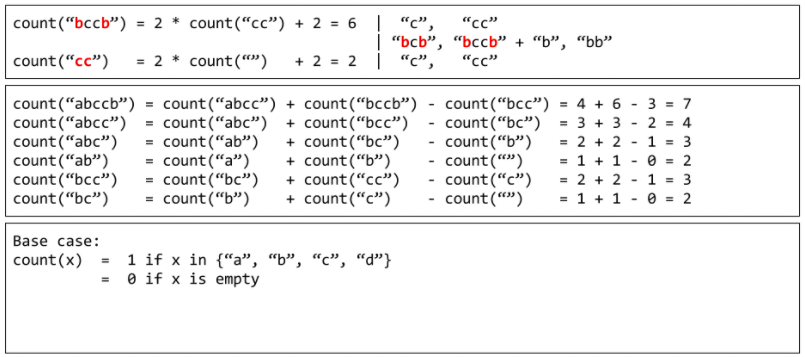
\includegraphics[width=.9\linewidth]{./pic/palindromSubSeq.png}

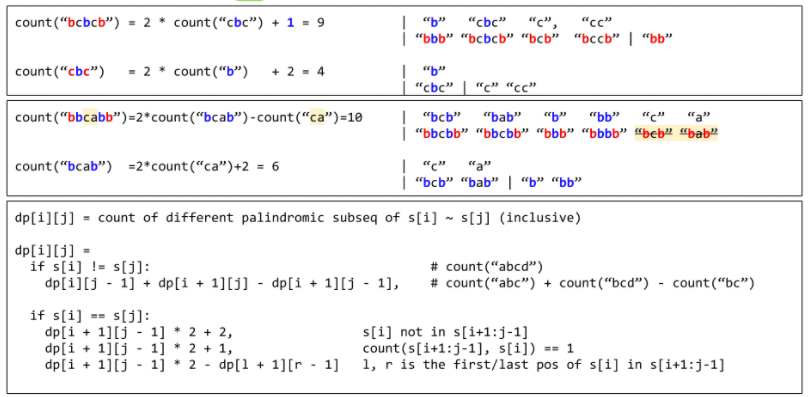
\includegraphics[width=.9\linewidth]{./pic/palindromSubSeq2.png}

\begin{minted}[fontsize=\scriptsize,linenos=false]{csharp}
private int dfs(char[] s, int i, int j) {
    if (i > j) return 0;
    if (i == j) return 1;
    if (dp[i][j] > 0) return dp[i][j];
    long ans = 0;
    if (s[i] == s[j]) {
        ans += dfs(s, i + 1, j - 1) * 2;
        int l = i + 1;
        int r = j - 1;
        while (l <= r && s[l] != s[i]) ++l;
        while (l <= r && s[r] != s[i]) --r;
        if (l > r) ans += 2;
        else if (l == r) ans += 1;
        else ans -= dfs(s, l + 1, r - 1);
    } else 
        ans = dfs(s, i, j - 1) + dfs(s, i + 1, j) - dfs(s, i + 1, j - 1);
    return dp[i][j] = (int)((ans + mod) % mod);
}
private static final int mod = (int)1e9 + 7;
private int [][] dp;
public int countPalindromicSubsequences(String S) {
    int n = S.length();
    dp = new int[n][n];
    return dfs(S.toCharArray(), 0, n - 1);
}
\end{minted}
\begin{itemize}
\item dp
\end{itemize}
\begin{minted}[fontsize=\scriptsize,linenos=false]{csharp}
public int countPalindromicSubsequences(String s) {
    int n = s.length();
    int mod = (int)1e9 + 7;
    char [] arr = s.toCharArray();
    long [][] dp = new long [n][n];
    for (int i = 0; i < n; i++) 
        dp[i][i] = 1;
    for (int len = 1; len <= n; len++) {
        for (int i = 0; i+len < n; i++) {
            int j = i + len;
            if (arr[i] == arr[j]) {
                dp[i][j] = dp[i+1][j-1] * 2;
                int l = i+1;
                int r = j-1;
                while (l <= r && arr[l] != arr[i]) ++l;
                while (l <= r && arr[r] != arr[i]) --r;
                if (l == r) dp[i][j] += 1;
                else if (l > r) dp[i][j] += 2;
                else dp[i][j] -= dp[l+1][r-1];
            } else dp[i][j] = dp[i][j-1] + dp[i+1][j] - dp[i+1][j-1];
            dp[i][j] = (dp[i][j] + mod) % mod;
        }
    }
    return (int)dp[0][n-1];
}
\end{minted}

\subsection{1125. Smallest Sufficient Team - Hard 这个题要多写几遍}
\label{sec-1-4-10}
In a project, you have a list of required skills req\_skills, and a list of people. The ith person people[i] contains a list of skills that the person has.

Consider a sufficient team: a set of people such that for every required skill in req\_skills, there is at least one person in the team who has that skill. We can represent these teams by the index of each person.

For example, team = [0, 1, 3] represents the people with skills people\footnotemark[1]{}, people\footnotemark[2]{}, and people\footnote{DEFINITION NOT FOUND.}.
Return any sufficient team of the smallest possible size, represented by the index of each person. You may return the answer in any order.

It is guaranteed an answer exists.
\begin{minted}[fontsize=\scriptsize,linenos=false]{csharp}
// 强行剪枝: 收集到的size >= 目前的结果,直接return;
// 这题的思路就是先把skill 和set of people建立好,
// 然后去用skill set做backtracking收集,如果temp team的size大于结果,直接return,否则update结果,
// 这里有个小tricky的地方,就是如果people是新人,加入之后dfs,backtracking的时候,要判断如果是新人,则remove,否则不remove;
private void dfs(String[] req_skills, HashSet<Integer> team, int idx) {
    if (team.size() >= minTeamSize) return; // 强行剪枝: 收集到的size >= 目前的结果,直接return;
    if (idx == req_skills.length) {
        minTeamSize = team.size();
        resTeam = new HashSet<Integer>(team);
        return;
    }
    boolean isNewPerson = false;
    for (int people : map.get(req_skills[idx])) {
        isNewPerson = team.add(people);
        dfs(req_skills, team, idx + 1);
        if (isNewPerson)
            team.remove(people);
    }
}
HashMap<String, Set<Integer>> map;
Set<Integer> resTeam; 
int minTeamSize;
public int[] smallestSufficientTeam(String[] req_skills, List<List<String>> people) {
    minTeamSize = people.size();
    this.map = new HashMap<>(); 
    for (int i = 0; i < minTeamSize; i++) 
        for (String skill: people.get(i)) 
            map.computeIfAbsent(skill, k -> new HashSet<Integer>()).add(i);
    this.resTeam = new HashSet<Integer>();
    dfs(req_skills, new HashSet<Integer>(), 0);
    int [] res = new int[resTeam.size()];     
    int idx = 0;
    for (int person : resTeam) 
        res[idx++] = person;
    return res;
}
\end{minted}
\begin{itemize}
\item Java soution using Bit DP 10ms
\end{itemize}
\begin{minted}[fontsize=\scriptsize,linenos=false]{csharp}
public int[] smallestSufficientTeam(String[] req_skills, List<List<String>> people) {
    int n = req_skills.length, range = 1 << n, cur, idx;
    Map<String, Integer> idxMap = new HashMap<>();
    for (int i = 0; i < n; i++) 
        idxMap.put(req_skills[i], i);
    long [] dp = new long [range]; // 每个bit位实际存了构成答案最小组的各成员的下标, 60个人, long
    int [] cnt = new int [range];
    Arrays.fill(cnt, Integer.MAX_VALUE);
    cnt[0] = 0;
    for (int i = 0; i < people.size(); i++) {
        List<String> l = people.get(i);
        cur = 0;
        for (String skill : l) 
            if (idxMap.containsKey(skill))
                cur |= 1 << idxMap.get(skill);
        for (int j = range-1; j > 0; j--) {
            idx = (j & cur) ^ j; // 由其它人所构成的拥有j的这些种技能的子集/ j的这些种技能可以由j一个人来替换(其它可能需要很多人才能最终拥有这些技能)
            if (cnt[idx] != Integer.MAX_VALUE && cnt[j] > cnt[idx] + 1) {
                cnt[j] = cnt[idx] + 1;
                dp[j] = dp[idx] | (1L << i); // at most 60 people
            }
        }
    }
    int [] res = new int[cnt[range-1]];
    long preRes = dp[range-1]; // 5 people: 11111, 1111, 111, 11, 1
    int valIdx = 0;
    long val = 0;
    idx = 0;
    while (preRes != 0) {
        val = preRes & 1;
        if (val == 1) res[idx++] = valIdx;
        preRes >>= 1;
        valIdx++;
    }
    return res;
}
\end{minted}
\begin{itemize}
\item DFS + Memorizaion (A real O(2\^{}skill * people) Solution) Java 8ms
\begin{itemize}
\item \url{https://leetcode.com/problems/smallest-sufficient-team/discuss/1011135/DFS-\%2B-Memorizaion}-(A-real-O(2skill-*-people)-Solution)-Java-8ms
\end{itemize}
\end{itemize}
\begin{minted}[fontsize=\scriptsize,linenos=false]{csharp}
List<Integer> minComb;
int[] peopleSkillMasks;
Integer[] memo;  // 这个方法确实快一点儿
int[] nextPerson;
int n;
public int[] smallestSufficientTeam(String[] req_skills, List<List<String>> people) {
    // 1. some preprocess to get bitmask for people skills
    this.n = req_skills.length;
    Map<String, Integer> skillToIdx = new HashMap<>();
    for (int i = 0; i < n; i++) 
        skillToIdx.put(req_skills[i], i);
    this.peopleSkillMasks = new int[people.size()];
    for (int i = 0; i < peopleSkillMasks.length; i++) {
        int skillMask = 0;
        for (String skill : people.get(i)) 
            skillMask |= (1 << skillToIdx.get(skill));
        peopleSkillMasks[i] = skillMask;
    }
    // 2. dfs
    memo = new Integer[1 << n];
    nextPerson = new int[1 << n];
    dfs(0, 0);
    // 3. reconstruct the path
    int curSkillSet = 0;
    List<Integer> res = new ArrayList<>();
    while(curSkillSet != (1 << n) - 1) {
        res.add(nextPerson[curSkillSet]);
        curSkillSet |= peopleSkillMasks[nextPerson[curSkillSet]];
    }
    return res.stream().mapToInt(i->i).toArray();
}
// a very simple dfs with memo to compute all combinations of people. 
// Use memorization to optimize the time complexity to O(2^skill * people) 2^skill for 2^skill node in the tree, people because each node has people computation
private int dfs(int curSkillSet, int startIdx) {
    if (curSkillSet == (1 << n) - 1) return 0;
    if (memo[curSkillSet] == null) {
        int res = Integer.MAX_VALUE / 2;
        int nextPersonIdx = -1;
        for (int i = startIdx; i < peopleSkillMasks.length; i++) {
            int withNewSkill = peopleSkillMasks[i] | curSkillSet; 
            if (withNewSkill != curSkillSet) {
                int numPeople = dfs(withNewSkill, i+1) + 1;
                if (res > numPeople) {
                    res = numPeople;
                    nextPersonIdx = i;
                }
            }
        }
        memo[curSkillSet] = res;
        nextPerson[curSkillSet] = nextPersonIdx; 
    }
    return memo[curSkillSet];
}
\end{minted}
\begin{itemize}
\item Recursion + Memoization + bit mask , with Simple JAVA solution
\begin{itemize}
\item \url{https://leetcode.com/problems/smallest-sufficient-team/discuss/1487180/Recursion-\%2B-Memoization-\%2B-bit-mask-with-Simple-JAVA-solution}
\end{itemize}
\end{itemize}
上面的这些方法相对较偏,就暂时顾不上了

\subsection{1575. Count All Possible Routes - Hard}
\label{sec-1-4-11}
You are given an array of distinct positive integers locations where locations[i] represents the position of city i. You are also given integers start, finish and fuel representing the starting city, ending city, and the initial amount of fuel you have, respectively.

At each step, if you are at city i, you can pick any city j such that j != i and 0 <= j < locations.length and move to city j. Moving from city i to city j reduces the amount of fuel you have by |locations[i] - locations[j]|. Please notice that |x| denotes the absolute value of x.

Notice that fuel cannot become negative at any point in time, and that you are allowed to visit any city more than once (including start and finish).

Return the count of all possible routes from start to finish.

Since the answer may be too large, return it modulo 10\^{}9 + 7.
\begin{minted}[fontsize=\scriptsize,linenos=false]{csharp}
// 自顶向下 (记忆化搜索)
// 每个dfs搜索当前状态为城市i,油量f到达终点的方案数。这样决策的时候就很直观:当前这个状态的方案数,由可去的城市的,且油量为剩余油量的到达终点方案数加起来。
// 初始化:每个状态都初始化为-1。
// 当走到终点时,这个状态的可走到终点的方案数+1。
private int dfs(int [] arr, int end, int idx, int fu) {
    if (dp[idx][fu] != -1) return dp[idx][fu];
    dp[idx][fu] = 0;
    if (idx == end) {
        dp[idx][fu] += 1;
        dp[idx][fu] %= mod;
    }
    for (int i = 0; i < n; i++) {
        if (i == idx || Math.abs(arr[i] - arr[idx]) > fu) continue;
        dp[idx][fu] = (dp[idx][fu] + dfs(arr, end, i, fu-Math.abs(arr[i]-arr[idx]))) % mod;
    }
    return dp[idx][fu];
}
int mod = (int)1e9 + 7;
int [][] dp;
int n;
public int countRoutes(int[] locations, int start, int finish, int fuel) {
    n = locations.length;
    if (fuel < Math.abs(locations[start] - locations[finish])) return 0;
    dp = new int[n][fuel+1];
    for (int i = 0; i < n; i++) 
        Arrays.fill(dp[i], -1);
    dfs(locations, finish, start, fuel);
    return dp[start][fuel];
}
// 自底向上
// 为什么想到动态规划:最优子结构:到达终点的方案数肯定由到达其他点的,不同油量的方案数求和。
//     如何定义状态:城市肯定在状态里,因为其他城市有不同的剩余油量的状态,且油量为0无法到达,也成为限制之一。所以油量也必须在状态里:
//     d p ( i , f ) dp(i, f)dp(i,f)表示到达第 i ii个城市,剩余油量为f ff 的方案数。
//     状态转移:第i ii个城市,可以由除本身外的城市转移过来,只要剩余的油量不小于所用的油量就够了,最后答案是求总共的个数,所以只要方案数相加就行:
//     dp(i,f−dist)=dp(i,f−dist)+dp(k,f)(f−dist>=0)
//     枚举顺序:每个城市肯定都要枚举一遍,因为还需要从另一个城市转移过来,所以除本身外的城市肯定还要再枚举一遍。
//     关键是油量的枚举,因为油量肯定是慢慢减少的,可以想到是逆序枚举,而且油量要放在最外层枚举。因为如果先枚举城市i ii,再枚举城市j jj,再枚举油量的话,只是不断更新了i ii城市方案数,而j jj城市不同油量的方案数根本没变化。
// dp:最优子结构 到达终点的方案数肯定由到达其他点的,不同油量的方案数求和
// 搜索:反过来 在第 i 个城市到达 fin 的方案数,也可以由其他的点到达 fin 的方案数转移过来, 但是油量有限制,所以油量肯定在状态里
// 所以城市 和 剩余油量肯定在状态里
// dp(i, j) 表示到达第 i 个城市,剩余油量为 j 的方案数
// dp(i, j) = dp(i, j) + dp(k, j - dist)
public int countRoutes(int[] locations, int start, int finish, int fuel) {
    int n = locations.length;
    if (fuel < Math.abs(locations[start] - locations[finish])) return 0;
    int [][] dp = new int[n][fuel+1];
    dp[start][fuel] = 1; // 初始点且燃料满的点方案数为1
    int leftFu = 0, mod = (int)1e9 + 7;
    for (int j = fuel; j >= 0; j--) { // fuel leftover
        for (int i = 0; i < n; i++) { // cur city
            for (int k = 0; k < n; k++) { // next city
                if (i == k) continue;
                leftFu = j - Math.abs(locations[i] - locations[k]);
                if (leftFu < 0) continue;
                dp[i][leftFu] = (dp[i][leftFu] + dp[k][j]) % mod; // 这里好别扭呀: 想呀想呀 
            }
        }
    }
    int ans = 0;
    for (int i = 0; i <= fuel; i++) 
        ans = (ans + dp[finish][i]) % mod;
    return ans;
}
\end{minted}

\subsection{1012. Numbers With Repeated Digits - Hard 数位DP + 压缩状态 经典}
\label{sec-1-4-12}
Given an integer n, return the number of positive integers in the range [1, n] that have at least one repeated digit.

题意:统计1-N中,满足每个位置都不同的数有几个。

思路:数位DP。通过一个1<<10的mask表示当前这个数,1-9哪些数被用了。

比赛的时候,一直想通过一个dfs直接找到不重复的数,一直不对。

赛后发现,别人都是通过一个dfs找重复的数,然后总个数减去。

\begin{minted}[fontsize=\scriptsize,linenos=false]{csharp}
private int dfs(int len, int limit, int mask) { // 不重复数的个数
    if (len == 0) return 1;
    if (limit == 0 && dp[len][mask][limit] > 0) return dp[len][mask][limit]; // 记忆化部分
    int maxn = limit > 0 ? bit[len] : 9; // 求出最高可以枚举到哪个数字
    int ans = 0;
    for (int i = 0; i <= maxn; i++)  // 当前位
        if ((mask&(1 << i)) == 0)
            if (mask == 0 && i == 0)
                ans += dfs(len - 1, (limit > 0 && i == maxn ? 1 : 0), mask); // 有前导0,所以0不能统计,不更新mask
            else ans += dfs(len - 1, (limit > 0 && i == maxn ? 1 : 0), mask | (1 << i)); // 更新mask
    if (limit == 0) dp[len][mask][limit] = ans; // 如果没有限制,代表搜满了,可以记忆化,否则就不能
    return ans;
}
int [][][] dp;
int [] bit;
public int numDupDigitsAtMostN(int N) {
    int sum = N + 1;
    bit = new int [19];
    dp = new int [19][1 << 10][2];
    int idx = 0;
    while (N > 0) {
        bit[++idx] = N % 10;
        N /= 10;
    }
    return sum - dfs(idx, 1, 0);
}
\end{minted}
\begin{enumerate}
\item 解题思路与分析: 降维一下 数位DP + 压缩状态 经典
\label{sec-1-4-12-1}
\begin{minted}[fontsize=\scriptsize,linenos=false]{csharp}
public int numDupDigitsAtMostN(int n) {
    if (n <= 10) return 0;
    int m = n + 1, r = 1 << 10, idx = 0; // r = 1 << 10 表示n值最多会有10个位,通过记忆化暴搜每个位的可能性、来数<=n的不重复数的个数
    d = new int[10]; // n 转化为数组
    while (n != 0) {
        d[idx++] = n % 10;
        n /= 10;
    }
    dp = new int [r][idx];
    for (int i = 0; i < r; i++) Arrays.fill(dp[i], -1);
    return m - dfs(idx-1, 0, 1); // 自底向上 
}
int [][] dp;
int [] d;  // dfs: 返回不得复数的个数
private int dfs(int idx, int r, int l) {   // l: limit flag: 当第一次搜到某数位,该数位能取的最大值是受限制的
    if (idx == -1) return 1;               // l: limit 有没有限制, 这个参数结合两种方法看得还是有些迷糊
    if (dp[r][idx] != -1 && l == 0) return dp[r][idx];
    int up = l == 1 ? d[idx] : 9, ans = 0; // 当前位的最大取值,求出当前位最高可以枚举到哪个数字
    for (int i = 0; i <= up; i++) { // 遍历当前位的所有可能的取值: [0, 1, 2, ... up]
        // 首先当前位的状态没有出现过 
        //(本体计算的是不满足 至少两次的所有情况 逆向思维) 
        if ((r & (1 << i)) == 0) { // 当前位第i位在r的状态里还没有出现过
            if (i == 0 && r == 0)  // 001的情况: 有前导 0, 所以 0 不能统计 , 不更新mask r(就是这个最高位为0的数不计入结果,去遍历下一个低位的数。。)
                ans += dfs(idx-1, r, 0);
            else // 当前数没有前导0、完全合法,计入结果,并进一步统计
                ans += dfs(idx-1, r | (1 << i), (l == 1 && i == d[idx] ? 1 : 0));
        }
    }
    if (l == 0) dp[r][idx] = ans; // 如果没有限制 , 代表搜满了 , 可以记忆化 , 否则就不能
    return ans;
}
\end{minted}
\item 解题思路与分析
\label{sec-1-4-12-2}

这道题给了一个正整数N,让返回所有不大于N且至少有一个重复数字的正整数的个数,题目中给的例子也可以很好的帮助我们理解。要求的是正整数的位数上至少要有一个重复数字,当然最简单暴力的方法就是从1遍历到N,然后对于每个数字判断是否有重复数字,看了一眼题目难度 Hard,想都不用想,肯定是超时的。这道题需要更高效的解法,首先来想,若是直接求至少有一个重复数字的正整数,由于并不知道有多少个重复数字,可能1个,2个,甚至全是重复数字,这样很难找到规律。有时候直接求一个问题不好求,可以考虑求其相反的情况,至少有一个重复数字反过来就是一个重复数字都没有,所以这里可以求不大于N且一个重复数字都没有的正整数的个数,然后用N减去这个数字即为所求。好,接下来看怎么求,对于任意一个N,比如 7918,是个四位数,而所有的三位数,两位数,一位数,都一定比其小,所以可以直接求出没有重复数字的三位数,两位数,和一位数。比如三位数,由于百位上不能有0,则只有9种情况,十位上可以有0,则有9种情况,个位上则有8种情况,所以就是 9*9*8。可以归纳出没有重复数字的n位数的个数,最高位去除0还有9种,剩余的 n-1 位则依次是 9,8,7\ldots{} 则后面的 n-1 位其实是个全排列,从9个数中取出 n-1 个数字的全排列,初中就学过的。这里写一个全排列的子函数,求从m个数字中取n个数字的全排列,方便后面计算。算完这些后,还要来算符合题意的四位数,由于第一位是7,若千位上是小于7的数字(共有6种,千位上不能是0),则后面的百位,十位,个位又都可以全排列了,从9个数字中取3个数字的全排列,再乘以千位上小于7的6种情况。若当千位固定为7,则百位上可以放小于9的数字(共有8种,百位不能放7,但可以放0),则后面的十位和个位都可以全排列了,从8个数字种取出2个数字的全排列,再乘以百位上小于9的8种情况。需要注意的是,遍历给定数字的各个位时,有可能出现重复数字,一旦出现了之后,则该 prefix 就不能再用了,因为已经不合题意了。所以要用一个 HashSet 来记录访问过的数字,一旦遇到重复数字后就直接 break 掉。最后还有一个小 trick 需要注意,由于N本身也需要计算进去,所以再计算的时候,使用 N+1 进行计算的话,就可以把N这种情况算进去了
\begin{minted}[fontsize=\scriptsize,linenos=false]{csharp}
private int A(int m, int n) {
    return n == 0 ? 1 : A(m, n-1) * (m-n+1);
}
public int numDupDigitsAtMostN(int n) {
    List<Integer> digits = new ArrayList<>();
    Set<Integer> vis = new HashSet<>();
    for (int i = n+1; i > 0; i /= 10) 
        digits.add(0, i % 10);
    int res = 0, m = digits.size();
    for (int i = 1; i < m; i++) res += 9 * A(9,  i-1);
    for (int i = 0; i < m; i++) {
        for (int j = i > 0 ? 0 : 1; j < digits.get(i); ++j) {
            if (vis.contains(j)) continue;
            res += A(9-i, m-i-1);
        }
        if (vis.contains(digits.get(i))) break;
        vis.add(digits.get(i));
    }
    return n - res;
}
\end{minted}
\end{enumerate}

\subsection{600. Non-negative Integers without Consecutive Ones - Hard}
\label{sec-1-4-13}
Given a positive integer n, return the number of the integers in the range [0, n] whose binary representations do not contain consecutive ones.
\begin{enumerate}
\item 解题思路与分析
\label{sec-1-4-13-1}

我们就可以通过DP的方法求出长度为k的二进制数的无连续1的数字个数。由于题目给我们的并不是一个二进制数的长度,而是一个二进制数,比如100,如果我们按长度为3的情况计算无连续1点个数个数,就会多计算101这种情况。所以我们的目标是要将大于num的情况去掉。下面从头来分析代码,首先我们要把十进制数转为二进制数,将二进制数存在一个字符串中,并统计字符串的长度。然后我们利用这个帖子中的方法,计算该字符串长度的二进制数所有无连续1的数字个数,然后我们从倒数第二个字符开始往前遍历这个二进制数字符串,如果当前字符和后面一个位置的字符均为1,说明我们并没有多计算任何情况,不明白的可以带例子来看。如果当前字符和后面一个位置的字符均为0,说明我们有多计算一些情况,就像之前举的100这个例子,我们就多算了101这种情况。我们怎么确定多了多少种情况呢,假如给我们的数字是8,二进制为1000,我们首先按长度为4算出所有情况,共8种。仔细观察我们十进制转为二进制字符串的写法,发现转换结果跟真实的二进制数翻转了一下,所以我们的t为"0001",那么我们从倒数第二位开始往前遍历,到i=1时,发现有两个连续的0出现,那么i=1这个位置上能出现1的次数,就到one数组中去找,那么我们减去1,减去的就是0101这种情况,再往前遍历,i=0时,又发现两个连续0,那么i=0这个位置上能出1的次数也到one数组中去找,我们再减去1,减去的是1001这种情况

\begin{minted}[fontsize=\scriptsize,linenos=false]{csharp}
public int findIntegers(int n) {
    int cnt = 0;
    String t = "";
    while (n > 0) {
        ++cnt;
        t += (n & 1) == 1 ? "1" : "0"; // 这里把t倒过来了
        n >>= 1;
    }
    char [] s = t.toCharArray();
    int [] one = new int [cnt], zero = new int [cnt];
    one[0] = zero[0] = 1;
    for (int i = 1; i < cnt; i++) {
        zero[i] = zero[i-1] + one[i-1];
        one[i] = zero[i-1];
    }
    int ans = zero[cnt-1] + one[cnt-1]; // 长度为cnt的所有不含重复1的数字的个数,但数多了
    for (int i = cnt-2; i >= 0; i--) {
        if (s[i] == '1' && s[i+1] == '1') break;
        if (s[i] == '0' && s[i+1] == '0') ans -= one[i];
    }
    return ans;
}
\end{minted}
\item 解题思路与分析
\label{sec-1-4-13-2}

其实长度为k的二进制数字符串没有连续的1的个数是一个斐波那契数列f(k)。比如当k=5时,二进制数的范围是00000-11111,我们可以将其分为两个部分,00000-01111和10000-10111,因为任何大于11000的数字都是不成立的,因为有开头已经有了两个连续1。而我们发现其实00000-01111就是f(4),而10000-10111就是f(3),所以f(5) = f(4) + f(3),这就是一个斐波那契数列啦。那么我们要做的首先就是建立一个这个数组,方便之后直接查值。我们从给定数字的最高位开始遍历,如果某一位是1,后面有k位,就加上f(k),因为如果我们把当前位变成0,那么后面k位就可以直接从斐波那契数列中取值了。然后标记pre为1,再往下遍历,如果遇到0位,则pre标记为0。如果当前位是1,pre也是1,那么直接返回结果。最后循环退出后我们要加上数字本身这种情况

\begin{minted}[fontsize=\scriptsize,linenos=false]{csharp}
public int findIntegers(int n) {
    int k = 31, pre = 0, ans = 0;
    int [] dp = new int [32];
    dp[0] = 1;
    dp[1] = 2;
    for (int i = 2; i < 32; i++) 
        dp[i] = dp[i-1] + dp[i-2];
    while (k >= 0) {
        if ((n & (1 << k)) > 0) {
            ans += dp[k];
            if (pre == 1) return ans;
            pre = 1;
        } else pre = 0;
        k--;
    }
    return ans + 1;
}
\end{minted}
\end{enumerate}

\subsection{514. Freedom Trail - Hard}
\label{sec-1-4-14}
In the video game Fallout 4, the quest "Road to Freedom" requires players to reach a metal dial called the "Freedom Trail Ring" and use the dial to spell a specific keyword to open the door.

Given a string ring that represents the code engraved on the outer ring and another string key that represents the keyword that needs to be spelled, return the minimum number of steps to spell all the characters in the keyword.

Initially, the first character of the ring is aligned at the "12:00" direction. You should spell all the characters in key one by one by rotating ring clockwise or anticlockwise to make each character of the string key aligned at the "12:00" direction and then by pressing the center button.

At the stage of rotating the ring to spell the key character key[i]:

You can rotate the ring clockwise or anticlockwise by one place, which counts as one step. The final purpose of the rotation is to align one of ring's characters at the "12:00" direction, where this character must equal key[i].
If the character key[i] has been aligned at the "12:00" direction, press the center button to spell, which also counts as one step. After the pressing, you could begin to spell the next character in the key (next stage). Otherwise, you have finished all the spelling.
\begin{enumerate}
\item 解题思路分析: dfs + 记忆数组(这个图把钥匙中每个字母的出现位置记住了,以后拿去用不搜)
\label{sec-1-4-14-1}
\begin{itemize}
\item 记录下所有字母对应的位置,这样在找字母相对位置的时候就不需要循环搜索了
\item 采用递归的方法,找出当前字母对应的位置最小的步数:只需要把当前字母对应的所有位置找出来,然后计算最小值即可
\item 下一个位置再次迭代计算即可
\end{itemize}
\begin{minted}[fontsize=\scriptsize,linenos=false]{csharp}
public int findRotateSteps(String ring, String key) { // dfs
    m = ring.length();
    n = key.length();
    char [] s = ring.toCharArray();
    for (int i = 0; i < m; i++) {
        if (key.indexOf(s[i]) == -1) continue; // 只记录在key中出现过的字母的位置
        idx.computeIfAbsent(s[i], z -> new ArrayList<>()).add(i);
    }
    dp = new int [m][n];
    return dfs(0, 0, ring, key);
}
Map<Character, List<Integer>> idx = new HashMap<>();
int [][] dp;
int m, n;
private int dfs(int i, int j, String s, String t) {
    if (j == n) return 0;
    if (dp[i][j] > 0) return dp[i][j];
    int ans = Integer.MAX_VALUE;
    for (Integer v : idx.get(t.charAt(j))) 
        ans = Math.min(ans, dfs(v, j+1, s, t) + getDist(v, i) + 1); // + 1 for confirm push
    return dp[i][j] = ans;
}
private int getDist(int i, int j) {
    int min = Math.min(i, j), max = Math.max(i, j);
    return Math.min(Math.abs(i - j), Math.abs(m - max + min)); 
}
\end{minted}
\item 解题思路分析 动态规划
\label{sec-1-4-14-2}
\begin{itemize}
\item 博主最先尝试的用贪婪算法来做,就是每一步都选最短的转法,但是OJ中总有些test case会引诱贪婪算法得出错误的结果,因为全局最优解不一定都是局部最优解,而贪婪算法一直都是在累加局部最优解,这也是为啥DP解法这么叼的原因。贪婪算法好想好实现,但是不一定能得到正确的结果。DP解法难想不好写,但往往才是正确的解法,这也算一个trade off吧。
\item 此题需要使用一个二维数组dp,其中dp[i][j]表示转动从i位置开始的key串所需要的最少步数(这里不包括spell的步数,因为spell可以在最后统一加上),此时表盘的12点位置是ring中的第j个字符。不得不佩服这样的设计的确很巧妙,我们可以从key的末尾往前推,这样dp\footnotemark[1]{}\textsuperscript{,}\,\footnotemark[1]{}就是我们所需要的结果,因为此时是从key的开头开始转动,而且表盘此时的12点位置也是ring的第一个字符。现在我们来看如何找出递推公式,对于dp[i][j],我们知道此时要将key[i]转动到12点的位置,而此时表盘的12点位置是ring[j],我们有两种旋转的方式,顺时针和逆时针,我们的目标肯定是要求最小的转动步数,而顺时针和逆时针的转动次数之和刚好为ring的长度n,这样我们求出来一个方向的次数,就可以迅速得到反方向的转动次数。为了将此时表盘上12点位置上的ring[j]转动到key[i],我们要将表盘转动一整圈,当转到key[i]的位置时,我们计算出转动步数diff,然后计算出反向转动步数,并取二者较小值为整个转动步数step,此时我们更新dp[i][j],更新对比值为step + dp[i+1][k],这个也不难理解,因为key的前一个字符key[i+1]的转动情况suppose已经计算好了,那么dp[i+1][k]就是当时表盘12点位置上ring[k]的情况的最短步数,step就是从ring[k]转到ring[j]的步数,也就是key[i]转到ring[j]的步数,用语言来描述就是,从key的i位置开始转动并且此时表盘12点位置为ring[j]的最小步数(dp[i][j])就等价于将ring[k]转动到12点位置的步数(step)加上从key的i+1位置开始转动并且ring[k]已经在表盘12点位置上的最小步数(dp[i+1][k])之和。
\item 突然发现这不就是之前那道Reverse Pairs中解法一中归纳的顺序重现关系的思路吗,都做了总结,可换个马甲就又不认识了,泪目中。。。
\end{itemize}
\begin{minted}[fontsize=\scriptsize,linenos=false]{csharp}
public int findRotateSteps(String ring, String key) { // dfs
    int m = key.length(), n = ring.length();
    char [] s = key.toCharArray();
    char [] t = ring.toCharArray();
    int [][] dp = new int [m+1][n];
    int dif = 0, cnt = 0;
    for (int i = m-1; i >= 0; i--) 
        for (int j = 0; j < n; j++) { // j 是固定在12点钟表盘的位置
            dp[i][j] = Integer.MAX_VALUE;
            for (int k = 0; k < n; k++) 
                if (s[i] == t[k]) {
                    dif = Math.abs(j - k);
                    cnt = Math.min(dif, n - dif);
                    dp[i][j] = Math.min(dp[i][j], cnt + dp[i+1][k]);
                }
        }
    return dp[0][0] + m;
}
\end{minted}

\item 解题思路分析: dfs + 记忆数组 todo: 这个写得太繁琐了,没看
\label{sec-1-4-14-3}

过程就是需要一步一步求key里面的每个字符。 如果当前位置已经是对应到这个字符,那么直接按按钮就可以

如果当前位置不是,那么有两种旋转方式,顺时针或者逆时针, 然后找到第一个字符就是在同一个方向上的最短距离,

因为在同一个方向上,即使后面有重复的字符,无论后面的字符在那里,遇到第一个符合条件的字符就按按钮一定是最优解。

但是在不同方向上就不一定了,有可能一个方向上当前字符距离更短,但是有可能后面的字符距离会更远,

比如ring=ABCDEFGBF , key=BG, 如果看第一个字符, 那应该是顺时针,只需要转一格就到,逆时针需要转两格,

但是顺时针第一步快了以后, 后面到G会需要更长的步骤。 而逆时针会比较快。

所以,基本的逻辑是每一步不能决定当前哪个方向是否是最优解, 只有不断递归,把每步的两个方向全部尝试完到key结束才可以

当然, 如果不做任何处理,这样做是要超时的(我开始就写了这样一个版本), 一个直观的做法,就是在递归的基础上

加一个记忆表, 针对ring的位置index和key的kindex做记录, 如果已经存在一个解了就可以直接返回结果

这个递归+memorization的解法,那一定存在一个bottom up的动态规划解法, 这个后面再学习

\begin{minted}[fontsize=\scriptsize,linenos=false]{csharp}
private int helper(String s, String t, int i, int j) { // s: ring, t: key, i: idxRing, j: idxKey
    Map<Integer, Integer> locMap = mem.get(i);
    if (locMap != null) 
        if (locMap.get(j) != null) return locMap.get(j);
    if (j == n) return 0;
    int step = 0, k = i;
    boolean foundK = false;
    for (; step <= m/2; ++step) {
        k = (i + step + m) % m;
        if (s.charAt(k) == t.charAt(j)) {
            foundK = true;
            break;
        }
    }
    int rstep = 0, x = i;
    boolean foundX = false;
    while (rstep <= m/2) {
        x = (i - rstep + m) % m;
        if (s.charAt(x) == t.charAt(j)) {
            foundX = true;
            break;
        }
        rstep++;
    }
    int min = Integer.MAX_VALUE;
    if (foundK) min = helper(s, t, k, j+1) + step + 1;
    if (foundX) min = Math.min(min, helper(s, t, x, j+1) + rstep + 1);
    if (locMap == null) {
        locMap = new HashMap<>();
        mem.put(i, locMap);
    }
    locMap.put(j, min);
    return min;
}
Map<Integer, Map<Integer, Integer>> mem = new HashMap<>();
int m, n;
public int findRotateSteps(String ring, String key) {
    m = ring.length();
    n = key.length();
    return helper(ring, key, 0, 0);
}
\end{minted}
\end{enumerate}

\subsection{78. Subsets - Medium 典型subset题目new ArrayList<>()\{\{add(v);\}\}}
\label{sec-1-4-15}
Given an integer array nums of unique elements, return all possible subsets (the power set).

The solution set must not contain duplicate subsets. Return the
solution in any order.
\begin{enumerate}
\item 解题思路与分析: Bitmasking
\label{sec-1-4-15-1}
\begin{minted}[fontsize=\scriptsize,linenos=false]{csharp}
public List<List<Integer>> subsets(int[] a) { // 这种应该是最简单最快的了
    int n = a.length, r = (1 << n);
    List<List<Integer>> ll = new ArrayList<>();
    for (int i = 0; i < r; i++) {
        List<Integer> l = new ArrayList<>();
        if (i == 0) {
            ll.add(l);
            continue;
        }
        for (int j = 0; j < n; j++) 
            if (((i >> j) & 1) == 1) l.add(a[j]);
        ll.add(l);
    }
    return ll;
}
\end{minted}
\item 解题思路与分析: Cascading
\label{sec-1-4-15-2}
\begin{minted}[fontsize=\scriptsize,linenos=false]{csharp}
public List<List<Integer>> subsets(int[] a) { // 在后面的动态规划中也会常用到,还是需要熟悉一下
    int n = a.length, r = (1 << n);
    List<List<Integer>> ll = new ArrayList<>();
    ll.add(new ArrayList<>());
    for (int v : a) {
        List<List<Integer>> tmp = new ArrayList<>();
        for (List<Integer> l : ll)
            tmp.add(new ArrayList<>(l) {{ add(v); }}); // 这种写法,见过一次,上次找了半天也没能找出来
        for (List<Integer>  l : tmp) 
            ll.add(l);
    }
    return ll;
}
\end{minted}
\item 解题思路与分析: backtracking
\label{sec-1-4-15-3}
\begin{minted}[fontsize=\scriptsize,linenos=false]{csharp}
public List<List<Integer>> subsets(int[] a) { // 这个最原始本能的、回溯的写法被我忘记了。。。。。。
    n = a.length;
    vis = new boolean [n];
    getASubset(new ArrayList<>(), 0, a);
    return ll;
}
List<List<Integer>> ll = new ArrayList<>();
boolean [] vis;
int n;
void getASubset(List<Integer> l, int idx, int [] a) {
    if (idx == n) {
        ll.add(new ArrayList<>(l));
        return ;
    }
    getASubset(l, idx+1, a);
    l.add(a[idx]);
    getASubset(l, idx+1, a);
    l.remove(l.size()-1);
}
\end{minted}
\end{enumerate}
\subsection{368. Largest Divisible Subset - Medium 要求返回序列的接龙型}
\label{sec-1-4-16}
Given a set of distinct positive integers nums, return the largest subset answer such that every pair (answer[i], answer[j]) of elements in this subset satisfies:

answer[i] \% answer[j] \texttt{= 0, or
answer[j] \% answer[i] =} 0
If there are multiple solutions, return any of them.
\begin{enumerate}
\item 解题思路与分析: 万能的dfs记忆化搜索
\label{sec-1-4-16-1}
\begin{minted}[fontsize=\scriptsize,linenos=false]{csharp}
public List<Integer> largestDivisibleSubset(int[] a) { // 出来一个新题: 恁是认不是它是dfs记忆化搜索,岂不是很悲催?
    Arrays.sort(a);
    n = a.length;
    dp = new List [n];
    for (int i = 0; i < n; i++) {
        List<Integer> cur = dfs(a, i, 1);
        if (cur.size() > ans.size())
            ans = cur;
    }
    return ans;
}
List<Integer> ans = new ArrayList<>();
List<Integer> [] dp;
int n;
// pre: dfs路径中前一节点
// 返回值:当前节点的倍数数组(包含当前节点)
private List<Integer> dfs(int [] a, int i, int pre) { 
    int cur = a[i];
    if (cur % pre != 0) return new ArrayList<>(); 
    if (dp[i] != null) return dp[i]; // 记忆数组存在当前结果的话直接返回,避免重复计算
    List<Integer> maxList = new ArrayList<>();
    for (int j = i+1; j < n; j++) {
        List<Integer> tmp = dfs(a, j, cur);
        if (tmp.size() > maxList.size())
            maxList = new ArrayList<>(tmp);
        // maxList = tmp; // bug: 
    }
    maxList.add(cur); // 将当前节点加入到集合中, 有点儿回溯的样子,把路径中的数字反序加了回来
    dp[i] = maxList;  // 将当前结果存入记忆数组
    return maxList;
}
\end{minted}
\item 解题思路与分析: 接龙型动态规划
\label{sec-1-4-16-2}

属于接龙型动态规划,类似于 Longest Increasing Subsequence 的做法。 这个题不同之处有两点:

需要记录具体方案O(N\^{}2) 的时间复杂度不能通过测试

具体的优化在于找上一个接龙的数的时候,不是 for 循环所有比他小的数,而是直接 for 循环他的因子。而获取因子可以用O(√n) 的时间做到。

\begin{minted}[fontsize=\scriptsize,linenos=false]{csharp}
public List<Integer> largestDivisibleSubset(int[] a) { // todo: 感觉想得还不是很透
    if (a == null || a.length == 0) return new ArrayList();
    Arrays.sort(a);
    int n = a.length;
    HashMap<Integer, Integer> dp = new HashMap();
    HashMap<Integer, Integer> pre = new HashMap();
    for (int i = 0; i < n; i++) {
        dp.put(a[i], 1);
        pre.put(a[i], -1);
    }
    int lastNum = a[0];
    for (int i = 0; i < n; i++) {
        int num = a[i];
        for (Integer factor : getFactors(num)) {
            if (!dp.containsKey(factor)) continue;
            if (dp.get(num) < dp.get(factor) + 1) {
                dp.put(num, dp.get(factor) + 1);
                pre.put(num, factor);
            }
        }
        if (dp.get(num) > dp.get(lastNum)) 
            lastNum = num;
    }
    return getPath(pre, lastNum);
}
private List<Integer> getPath(HashMap<Integer, Integer> pre, int lastNum) {
    List<Integer> path = new ArrayList();
    while (lastNum != -1) {
        path.add(lastNum);
        lastNum = pre.get(lastNum);
    }
    Collections.reverse(path);
    return path;
}
private List<Integer> getFactors(int num) {
    List<Integer> factors = new ArrayList();
    if (num == 1) return factors;
    int factor = 1;
    while (factor * factor <= num) {
        if (num % factor == 0) {
            factors.add(factor);
            if (factor != 1 && num / factor != factor) // 这里会把所有质因子的倍数也加进去,怕数组中不存在最小质因子,而是存在其某个倍数?
                factors.add(num / factor);
        }
        factor++;
    }
    return factors;
}
\end{minted}
\item 解题思路与分析: 一个极为简洁的dp
\label{sec-1-4-16-3}

这里有个很简单的数学性质,就是整除的传递性,如果a\%b==0 且 b\%c \texttt{= 0,那么a\%c =} 0,说白了如果c是b的因子,b又是a的因子,那么c肯定是a的因子。这样我们就可以在数组中找出很多整除链(a->b->c->d,其中b是a的因子,c是b的因子,d是c的因子),这样的链条就满足两两整除的条件,题目就变成了求最长的链条。

\begin{minted}[fontsize=\scriptsize,linenos=false]{csharp}
public List<Integer> largestDivisibleSubset(int[] nums) {
    int n = nums.length;
    List<Integer> ans = new ArrayList<Integer>();
    if (n < 2) {
        if (n == 0) return ans;
        ans.add(nums[0]);
        return ans;
    }
    Arrays.sort(nums);
    int[] preFactIdx = new int[n];
    int[] factCnt = new int[n];
    int maxlength = 0;
    int maxnum = 0;
    for (int i = n-1; i >= 0; i--) 
        for (int j = i; j < n; j++) 
            if (nums[j] % nums[i] == 0 && factCnt[i] < factCnt[j]+1) {
                factCnt[i] = factCnt[j]+1;
                preFactIdx[i] = j;
                if (factCnt[i] > maxlength) {
                    maxlength = factCnt[i];
                    maxnum = i;
                }
            }
    for (int i = 0; i < maxlength; i++) {
        ans.add(nums[maxnum]);
        maxnum = preFactIdx[maxnum];
    }
    return ans;
}
\end{minted}

首先我先对nums排序,这里我用了两个数组prefactors[]和factorcount[],prefactors[i]里其实保存的是以nums[i]未结尾的整除链前面一个数的下标,factorcount[i]存的是以nums[i]结尾的整除链长度。这里我们就可以用动态规划的方式求出factorcount[i]的值了,取最大的一个,然后再根据prefactors[i]推算出整除链中所有的元素。

  这里开两个脑洞,发散下思维。

\begin{itemize}
\item 脑洞1:  其实所有整除链可以合并为一个多叉整除树,这里得增加一个额外的根节点,使得根节点可以被nums中任何一个数整除。这个整除树有个很重要的性质——除根节点以为任意节点可以整除其父节点。 这道题就会演变成求整除树中最深的路径。 对于树的问题,我们往往能用递归的方式解决,代码也会变得比较好理解。
\item 脑洞2:  看下代码,是不是很像01背包,其实我觉得这到题可以认为是带限制条件的01背包,限制条件可以简化为放入背包的数必须能整除背包中最小的一个数,背包为无穷大,每个数的价值为1。
\end{itemize}
\end{enumerate}

\subsection{673. Number of Longest Increasing Subsequence}
\label{sec-1-4-17}
Given an integer array nums, return the number of longest increasing subsequences.
Notice that the sequence has to be strictly increasing.
\begin{minted}[fontsize=\scriptsize,linenos=false]{csharp}
public int findNumberOfLIS(int[] nums) { // dynamic programming
    int n = nums.length;
    int [][] arr = new int[n][2];
    int maxLength = 1;
    for (int i = 0; i < n; i++) 
        Arrays.fill(arr[i], 1);
    for (int i = 0; i < n; i++) {
        for (int j = i+1; j < n; j++) {
            if (nums[j] > nums[i]) {
                if (arr[i][0] + 1 > arr[j][0]) {
                    arr[j][0] = arr[i][0] +1;
                    arr[j][1] = arr[i][1];
                    maxLength = Math.max(maxLength, arr[j][0]);
                } else if (arr[i][0] + 1 == arr[j][0])
                    arr[j][1] += arr[i][1];
            }
         }
    }
    int cnt = 0;
    for (int i = 0; i < n; i++) 
        if (arr[i][0] == maxLength) cnt += arr[i][1];
    return cnt;
}
\end{minted}

\subsection{1987. Number of Unique Good Subsequences - Hard}
\label{sec-1-4-18}
You are given a binary string binary. A subsequence of binary is considered good if it is not empty and has no leading zeros (with the exception of "0").

Find the number of unique good subsequences of binary.

For example, if binary = "001", then all the good subsequences are ["0", "0", "1"], so the unique good subsequences are "0" and "1". Note that subsequences "00", "01", and "001" are not good because they have leading zeros.
Return the number of unique good subsequences of binary. Since the answer may be very large, return it modulo 109 + 7.

A subsequence is a sequence that can be derived from another sequence by deleting some or no elements without changing the order of the remaining elements.

这里的思路是:扫出从左起第一个1所在的位置,从左到右遍历,对于当前字符来说就是 \textbf{用} 当前字符或 \textbf{不用} 当前字符两种选择,然后会有重复的部分,需要把重复的部分减掉
\begin{minted}[fontsize=\scriptsize,linenos=false]{csharp}
小写字母a的ascii编码值为97,小写字母z的ascii编码值为122,
将数字97表示为小写字母a,那么每一个字母都可以由97+i来表示,i=0~25
例如 b --> 97+1
所以,dp[i]的下标i就能用来表示字母97+i,这样只需要26个空间即可表示所有的26个字母
然后dp[i],这里表示的是以97+i结尾的子序列的个数
下面是对字符串S,从左到右进行遍历
这样的遍历,有这样的特点,以字符串"abcsade"为例子来描述
当遍历到字符s的时候,显然前面的字符"abc"都已经遍历了一次,
注意!子问题出现 : 
假设前面的"abc",已经找出了所有的不重复的子序列:a,b,c,ab,ac,bc
那么当遍历到's'时,这个's'可以添加到所有上述子序列的末尾,构成新的子序列
由于原子序列不重复,显然在其所有子序列后添加一个字符's'得到的新的一系列子序列,
依然是不重复的。
所以能发现,以's'结尾的新的子序列实际就是上述这些末尾添加了's'的子序列
但是考虑到's'字符可以单独作为一个子序列,因此还需要加上1,表示这一特例
那么总结上述推断,假设dp[i]表示当前遍历到字符97+i时,以此字符结尾的子序列的个数
dp[i] = 1+dp[0]+dp[1]+dp[2]+...+dp[i-1] = 1+sum(dp)
\end{minted}

\begin{minted}[fontsize=\scriptsize,linenos=false]{csharp}
public int numberOfUniqueGoodSubsequences(String binary) {
    int mod = (int)1e9 + 7;
    int n = binary.length(), preZoo = 0, preOne = 0, m = 1;
    long [] dp = new long [n+1];
    String s = "#" + binary;
    while (m <= n && s.charAt(m) == '0') m++;
    if (m == n+1) return 1;
    dp[m] = 1;
    preOne = m;
    preZoo = m-1;
    for (int i = m+1; i <= n; i++) {
        char c = s.charAt(i);
        int j = (c == '0' ? preZoo : preOne);
        dp[i] = (2 * dp[i-1] % mod - (j >= 1 ? dp[j-1] : 0) + mod) % mod;
        if (c == '0') preZoo = i;
        else preOne = i;
    }
    return (int)dp[n] + (s.indexOf("0") != -1 ?  1 : 0);
}
\end{minted}
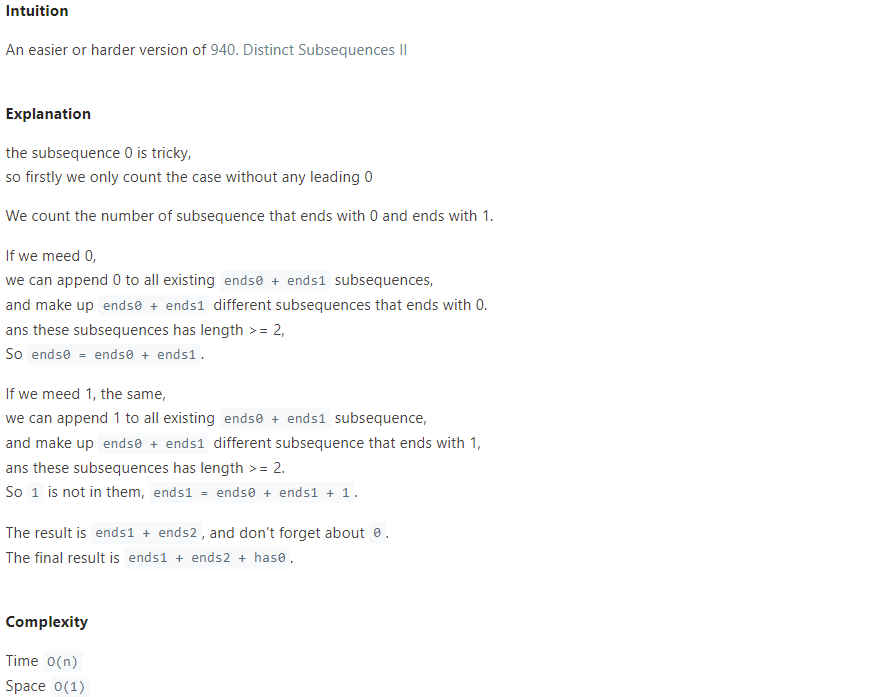
\includegraphics[width=.9\linewidth]{./pic/distinctSubsequence.png}
\begin{minted}[fontsize=\scriptsize,linenos=false]{csharp}
public int numberOfUniqueGoodSubsequences(String binary) {
    int mod = (int)1e9 + 7;
    int endZoo = 0, endOne = 0, hasZoo = 0;
    for (int i = 0; i < binary.length(); i++) 
        if (binary.charAt(i) == '1')
            endOne = (endOne + endZoo + 1) % mod;
        else {
            endZoo = (endZoo + endOne) % mod;
            hasZoo = 1;
        }
    return (endOne + endZoo + hasZoo) % mod;
}
\end{minted}
\begin{itemize}
\item 还有一个没有看懂的
\begin{itemize}
\item \url{https://leetcode-cn.com/problems/number-of-unique-good-subsequences/solution/ju-yi-fan-san-by-avenger-h-34xa/}
\item \url{https://leetcode-cn.com/problems/distinct-subsequences-ii/solution/dong-tai-gui-hua-cong-fen-xi-dao-shi-xian-by-my10y/}
\end{itemize}
\end{itemize}
\begin{minted}[fontsize=\scriptsize,linenos=false]{python}
def numberOfUniqueGoodSubsequences(self, binary: str) -> int:
        M = 10**9+7
        dp = [0]*10
        b = str(int(binary))
        l = len(binary) - len(b)
        if l > 0:
            dp[0] = 1
        for c in b:
            if dp[0] >= 1:
                dp[int(c)] = (sum(dp)) % M
            else:
                dp[int(c)] = ( 1+ sum(dp)) % M
        return sum(dp)%M
\end{minted}
\subsection{714. Best Time to Buy and Sell Stock with Transaction Fee}
\label{sec-1-4-19}
You are given an array prices where prices[i] is the price of a given stock on the ith day, and an integer fee representing a transaction fee.
Find the maximum profit you can achieve. You may complete as many transactions as you like, but you need to pay the transaction fee for each transaction.
Note: You may not engage in multiple transactions simultaneously (i.e., you must sell the stock before you buy again).
\begin{minted}[fontsize=\scriptsize,linenos=false]{csharp}
public int maxProfit(int[] prices, int fee) {
    int n = prices.length;
    int [] sold = new int[n];
    int [] hold = new int[n];
    hold[0] = -prices[0];
    for (int i = 1; i < n; i++) {
        sold[i] = Math.max(sold[i-1], hold[i-1]+prices[i]-fee);
        hold[i] = Math.max(hold[i-1], sold[i-1]-prices[i]);
    }
    return sold[n-1];
}
\end{minted}

\subsection{847. Shortest Path Visiting All Nodes}
\label{sec-1-4-20}
You have an undirected, connected graph of n nodes labeled from 0 to n - 1. You are given an array graph where graph[i] is a list of all the nodes connected with node i by an edge.
Return the length of the shortest path that visits every node. You may start and stop at any node, you may revisit nodes multiple times, and you may reuse edges.
\begin{minted}[fontsize=\scriptsize,linenos=false]{csharp}
public int shortestPathLength(int[][] graph) {
    int n = graph.length;
    int tar = 0, res = 0;
    HashSet<String> s = new HashSet<>();
    Queue<Pair<Integer, Integer>> q = new LinkedList<>();
    for (int i = 0; i < n; i++) {
        int mask = (1 << i);
        tar |= mask;
        s.add(Integer.toString(mask) + "-" + Integer.toString(i));
        q.add(new Pair<>(mask, i));
    }
    while (!q.isEmpty()) {
        for (int i = q.size(); i > 0; i--) {
            Pair cur = q.remove();
            if ((int)cur.getKey() == tar) return res;
            for (int next : graph[(int)cur.getValue()]) {
                int path = (int)cur.getKey() | (1 << next);
                String str = Integer.toString(path) + "-" + Integer.toString(next);
                if (s.contains(str)) continue;
                s.add(str);
                q.add(new Pair<>(path, next));
            }
        }
        ++res;
    }
    return -1;
}
\end{minted}

\subsection{926. Flip String to Monotone Increasing - Medium}
\label{sec-1-4-21}
A binary string is monotone increasing if it consists of some number of 0's (possibly none), followed by some number of 1's (also possibly none).

You are given a binary string s. You can flip s[i] changing it from 0 to 1 or from 1 to 0.

Return the minimum number of flips to make s monotone increasing.
\begin{enumerate}
\item 解题思路与分析:动态规划
\label{sec-1-4-21-1}

这道题给了我们一个只有0和1的字符串,现在说是可以将任意位置的数翻转,即0变为1,或者1变为0,让组成一个单调递增的序列,即0必须都在1的前面,博主刚开始想的策略比较直接,就是使用双指针分别指向开头和结尾,开头的指针先跳过连续的0,末尾的指针向前跳过连续的1,然后在中间的位置分别记录0和1的个数,返回其中较小的那个。这种思路乍看上去没什么问题,但是实际上是有问题的,比如对于这个例子 "10011111110010111011",如果按这种思路的话,就应该将所有的0变为1,从而返回6,但实际上更优的解法是将第一个1变为0,将后4个0变为1即可,最终可以返回5.

这说明了之前的解法是不正确的。这道题可以用动态规划 Dynamic Programming 来做,需要使用两个 dp 数组,其中 cnt1[i] 表示将范围是 [0, i-1] 的子串内最小的将1转为0的个数,从而形成单调字符串。同理,cnt0[j] 表示将范围是 [j, n-1] 的子串内最小的将0转为1的个数,从而形成单调字符串。这样最终在某个位置使得 cnt0[i]+cnt1[i] 最小的时候,就是变为单调串的最优解,这样就可以完美的解决上面的例子,子串 "100" 的最优解是将1变为0,而后面的 "11111110010111011" 的最优解是将4个0变为1,总共加起来就是5,参见代码如下:

\begin{minted}[fontsize=\scriptsize,linenos=false]{csharp}
// 可以用动态规划 Dynamic Programming 来做,需要使用两个 dp 数组,其中 cnt1[i] 表示将范围是 [0, i-1] 的子串内最小的将1转为0的个数,从而形成单调字符串。
// 同理,cnt0[j] 表示将范围是 [j, n-1] 的子串内最小的将0转为1的个数,从而形成单调字符串。
// 这样最终在某个位置使得 cnt0[i]+cnt1[i] 最小的时候,就是变为单调串的最优解,
public int minFlipsMonoIncr(String t) { // bug
    int n = t.length(), ans = Integer.MAX_VALUE;
    char [] s = t.toCharArray();
    int [] l = new int [n+1], r = new int [n+1];
    for (int i = 1, j = n-1; i <= n; i++, --j) {
        l[i] = l[i-1] + (s[i-1] == '0' ? 0 : 1); // cnt left --> right 1--> 0
        r[j] = r[j+1] + (s[j] == '0' ? 1 : 0);
    }
    for (int i = 0; i <= n; i++) 
        ans = Math.min(l[i] + r[i], ans);
    return ans;
}
\end{minted}
\item 解题思路与分析: 空间压缩与简化
\label{sec-1-4-21-2}

我们可以进一步优化一下空间复杂度,用一个变量 cnt1 来记录当前位置时1出现的次数,同时 res 表示使到当前位置的子串变为单调串的翻转次数,用来记录0的个数,因为遇到0就翻1一定可以组成单调串,但不一定是最优解,每次都要和 cnt1 比较以下,若 cnt1 较小,就将 res 更新为 cnt1,此时保证了到当前位置的子串变为单调串的翻转次数最少,并不关心到底是把0变为1,还是1变为0了,其实核心思想跟上面的解法很相近

\begin{minted}[fontsize=\scriptsize,linenos=false]{csharp}
// 用一个变量 cnt1 来记录当前位置时1出现的次数,同时 res 表示使到当前位置的子串变为单调串的翻转次数,
// 用来记录0的个数,因为遇到0就翻1一定可以组成单调串,但不一定是最优解,
// 每次都要和 cnt1 比较以下,若 cnt1 较小,就将 res 更新为 cnt1,
// 此时保证了到当前位置的子串变为单调串的翻转次数最少,并不关心到底是把0变为1,还是1变为0了
public int minFlipsMonoIncr(String t) { // bug
    int n = t.length(), res = 0, cntOne = 0;
    char [] s = t.toCharArray();
    for (int i = 0; i < n; i++) {
        if (s[i] == '0') res++;
        else cntOne++;
        res = Math.min(res, cntOne);
    }
    return res;
}
\end{minted}

早上的时候不是刚写过一个这样的题吗 ? 与1493 的第二种解法有什么区别?
\end{enumerate}

\subsection{1931. Painting a Grid With Three Different Colors}
\label{sec-1-4-22}
You are given two integers m and n. Consider an m x n grid where each cell is initially white. You can paint each cell red, green, or blue. All cells must be painted.
Return the number of ways to color the grid with no two adjacent cells having the same color. Since the answer can be very large, return it modulo 109 + 7.
\begin{itemize}
\item lightweighted轻巧点儿的解题方案: bitmask
\end{itemize}
\begin{minted}[fontsize=\scriptsize,linenos=false]{csharp}
// time O( (2^5) *2 * N)
// SPACE O(N)
//     For m = 5, there are at most 48 valid states for a single column so we can handle it column by column.
//     We encode the color arrangement by bit mask (3 bit for a position) and use dfs to generate the all valid states.
//         Then for each column, we iterator all the states and check if its still valid with the previous column.
public void helper(int m, int pos, HashMap<Integer, Long> dic, int pre, int cur) {
    if (pos == m) {
        dic.put(cur, 1L);
        return;
    }
    //不需要{1, 2, 4} {0, 1, 2} is ok 每个格(实际占用3个bit)
    for (int i = 0; i < 3; i++) {
        if (i == pre) continue; 
        helper(m, pos + 1, dic, i, (cur << 3) | (1 << i)); // 每处理一格,将当前状态左移3位?(实际每个格占用3个bit位)| 现在这个格的值?这个,我好昏呀
    }
}
static int mod = (int) 1e9 + 7;
public int colorTheGrid(int m, int n) {
    HashMap<Integer,Long> dic = new HashMap<>();
    helper(m, 0, dic, -1, 0);     // 这应该就是我想找的精巧不占多少空间的mask了,可是有点儿看不懂
    HashSet<Integer> set = new HashSet<>(dic.keySet());
    for (int i = 1; i < n; i++) { // 动态规划: 用两个图像滚动数组一样轮流记载得出答案
        HashMap<Integer, Long> tmp = new HashMap<>();
        for (int x: set) 
            for (int y : set) 
                if ((x & y) == 0) // 相邻涂色方案为有效方案
                    tmp.put(y, (tmp.getOrDefault(y, 0L) + dic.get(x)) % mod);
        dic = tmp;
    }
    long res = 0L;
    for (Long x : dic.values()) {
        res += x;
        res %= mod;
    }
    return (int) res;
}
\end{minted}
\begin{itemize}
\item 比较传统一点儿的解法,思路清晰
\end{itemize}
\begin{minted}[fontsize=\scriptsize,linenos=false]{csharp}
// 参考的答案里,这个最逻辑简单、通俗大众易懂,但稍显笨重,两个图,用一个链表来记忆一行的涂色方案,如果有更精巧一点儿的bitmask,是我想找的答案
// https://leetcode.com/problems/painting-a-grid-with-three-different-colors/discuss/1334366/Easy-Java-comments-28ms-O(n*P*P)-complexity-memory-O(P)-where-P-is-column-permutations-count 这个又稍嫌太偏了,考得极少,不易懂,容易出错,可是bitmask又只能set 1 or 0,BitSet()可以吗?
// 先预处理得到单行的所有有效涂色方案,
// 再进一步计算得到每种单行方案对应的有效邻行方案
// 在此基础上,结合动态规划方法,逐行求解各种涂色状态对应的方案总数,最后统计得到总方案数。
public int colorTheGrid(int m, int n) {
// 获得单行所有涂色方案
    Map<Integer, List<Integer>> line = new HashMap<>(); //  3^m ways of paying one row
    int range = (int)Math.pow(3, m); // 用0、1、2表示各个网格的颜色,key为方案对应的数值,value为方案对应的数组
    for (int i = 0; i < range; i++) {
        List<Integer> list = new ArrayList<>(); //  val val values (0, 1, 2) of every m cols into list
        int val = i;
        for (int j = 0; j < m; j++) {
            list.add(val % 3);
            val /= 3;
        }
        boolean valid = true; // 确认该数组中是否存在相邻位置颜色相同
        for (int j = 1; j < m; j++) 
            if (list.get(j-1) == list.get(j)) {
                valid = false;
                break;
            }
        if (valid) line.put(i, list); // 相邻网格颜色均不同,为有效方案,加入哈希表
    }
// 预处理得到每种单行方案对应的有效邻行方案
    Map<Integer, List<Integer>> adj = new HashMap<>();
    Iterator it = line.entrySet().iterator();
    while (it.hasNext()) {     //  3^m ways of paying one row
        Map.Entry entry = (Map.Entry)it.next();
        int va = (int)entry.getKey();
        List<Integer> lva = (List<Integer>)entry.getValue();
        adj.put(va, new ArrayList<Integer>());
        Iterator itb = line.entrySet().iterator();
        while (itb.hasNext()) { //  3^m ways of paying one row
            Map.Entry enb = (Map.Entry)itb.next(); 
            int vb = (int)enb.getKey();
            List<Integer> lvb = (List<Integer>)enb.getValue();
            boolean valid = true;
            for (int i = 0; i < m; i++) 
                if (lva.get(i) == lvb.get(i)) {
                    valid = false;
                    break;
                } // among 3^m ways of painting one row, how many is valid, and valid mask into adj.get(va);
            if (valid) adj.get(va).add(vb); 
        }
    }
// 动态规划,逐行求解方案数
    int mod = (int)(1e9+7);
    long [] dp = new long [range];  // 上一行各种涂色方案对应的总方法数
    for (int i = 0; i < range; i++) // 初始化
        dp[i] = line.containsKey(i) ? 1 : 0;
    for (int i = 1; i < n; i++) {   // 从第二行开始动态规划
        long [] cur = new long [range];  // 新一行各种涂色方案对应的总方法数
        for (int j = 0; j < range; j++) 
            if (adj.containsKey(j)) {    // 该方案有效
                for (int v : adj.get(j)) // 遍历有效的相邻方案
                    cur[j] = (cur[j] + dp[v]) % mod; // 总方法数累加
            }
        System.arraycopy(cur, 0, dp, 0, range);
    }
    long ans = 0;
    for (int i = 0; i < range; i++) 
        ans = (ans + dp[i]) % mod;
    return (int)ans;
}
\end{minted}

\subsection{313. Super Ugly Number}
\label{sec-1-4-23}
A super ugly number is a positive integer whose prime factors are in the array primes.
Given an integer n and an array of integers primes, return the nth super ugly number.
The nth super ugly number is guaranteed to fit in a 32-bit signed integer.
\begin{minted}[fontsize=\scriptsize,linenos=false]{csharp}
static class Node implements Comparable<Node> {
    private int index;
    private int val;
    private int prime;
    public Node(int index, int val, int prime) {
        this.index = index;
        this.val = val;
        this.prime = prime;
    }
    public int compareTo(Node other) {
        return this.val - other.val;
    }
}
public int nthSuperUglyNumber(int n, int[] primes) {
    final int [] arr = new int[n];
    arr[0] = 1;              // 1 is the first ugly number
    final Queue<Node> q = new PriorityQueue<>();
    for (int i = 0; i < primes.length; ++i) 
        q.add(new Node(0, primes[i], primes[i]));
    for (int i = 1; i < n; ++i) {
        Node node = q.peek(); // get the min element and add to arr
        arr[i] = node.val;
        do {             // update top elements
            node = q.poll();
            node.val = arr[++node.index] * node.prime;
            q.add(node); // push it back
        } while (!q.isEmpty() && q.peek().val == arr[i]); // prevent duplicate
    }
    return arr[n - 1];
}
\end{minted}
\begin{itemize}
\item 下面这种解法也很巧妙
\end{itemize}
\begin{minted}[fontsize=\scriptsize,linenos=false]{csharp}
public int nthSuperUglyNumber(int n, int[] primes) {
    int m = primes.length;
    int [] ans = new int[n]; // 存放1-n个SuperUglyNumber
    ans[0] = 1;              // 第一个SuperUglyNumber是1
    int [] next = new int[m];
    for (int i=0; i < m; i++)
        next[i] = 0;         // 初始化
    int cnt = 1, min = Integer.MAX_VALUE, tmp = 0;
    while (cnt < n) {
        min = Integer.MAX_VALUE;
        for (int i = 0; i < m; i++){
             tmp = ans[next[i]] * primes[i];
             min = Math.min(min, tmp);
        }
        for (int i = 0; i < m; i++)
            if (min == ans[next[i]] * primes[i])
                next[i]++;
        ans[cnt++] = min;			
    }
    return ans[n-1];		
}
\end{minted}

\subsection{backpack III}
\label{sec-1-4-24}
\begin{minted}[fontsize=\scriptsize,linenos=false]{csharp}
public int backPackIII(int[] A, int[] V, int m) {
    int n = A.length;
    int [] dp = new int[m+1];
    for (int i = 1; i <= m; i++) {
        for (int j = 0; j < n; j++) {
            if (i - A[j] >= 0)
                dp[i] = Math.max(dp[i], dp[i-A[j]] + V[j]);
        }
    }
    return dp[m];
}
\end{minted}

\subsection{879. Profitable Schemes - Hard 0-1背包问题}
\label{sec-1-4-25}
There is a group of n members, and a list of various crimes they could commit. The ith crime generates a profit[i] and requires group[i] members to participate in it. If a member participates in one crime, that member can't participate in another crime.

Let's call a profitable scheme any subset of these crimes that generates at least minProfit profit, and the total number of members participating in that subset of crimes is at most n.

Return the number of schemes that can be chosen. Since the answer may be very large, return it modulo 109 + 7.
\begin{enumerate}
\item 解题思路与分析: DP
\label{sec-1-4-25-0-1}

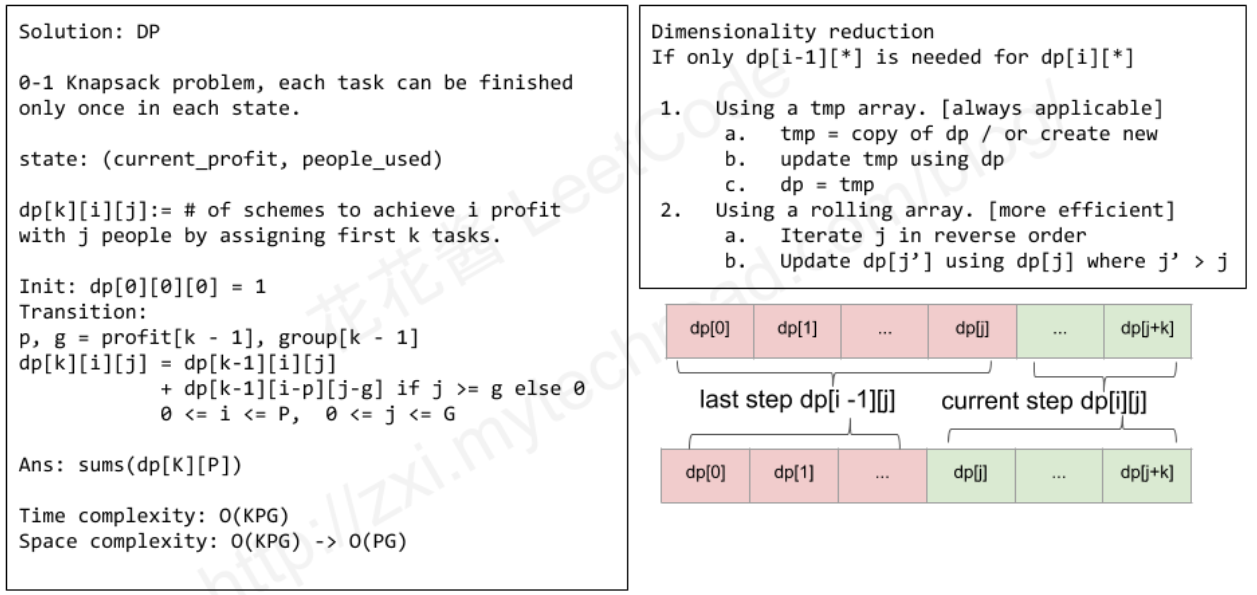
\includegraphics[width=.9\linewidth]{./pic/crime.png}

\begin{itemize}
\item 题目中说了结果可能非常大,要对一个超大数取余,看到这里,我们也就该明白为了不爆栈,只能用动态规划 Dynamic Programming 来做,LeetCode 里有好多题都是要对这个 1e9+7 取余,不知道为啥都是对这个数取余。Anyway,who cares,还是来想想 dp 数组如何定义以及怎么推导状态转移方程吧。
\end{itemize}

首先来看分配黑帮资源时候都需要考虑哪些因素,总共有三点,要干几票买卖,要用多少人,能挣多少钱。所以我们需要一个三维的 dp 数组,其中 dp[k][i][j] 表示最多干k票买卖,总共用了i个人,获得利润为j的情况下分配方案的总数,初始化 dp\footnotemark[1]{}\textsuperscript{,}\,\footnotemark[1]{}\textsuperscript{,}\,\footnotemark[1]{} 为1。

现在来推导状态转移方程,整个规划的核心是买卖,总共买卖的个数是固定的,每多干一票买卖,可能的分配方法就可能增加,但不可能减少的,因为假如当前已经算出来做 k-1 次买卖的分配方法总数,再做一次买卖,之前的分配方法不会减少,顶多是人数不够,做不成当前这票买卖而已,所以我们的 dp[k][i][j] 可以先更新为 dp[k-1][i][j],然后再来看这第k个买卖还能不能做,我们知道假设这第k个买卖需要g个人,能获得利润p,只有当我们现在的人数i大于等于g的时候,才有可能做这个任务,我们要用g个人来做任务k的话,那么其余的 k-1 个任务只能由 i-g 个人来做了,而且由于整个需要产生利润j,第k个任务能产生利润p,所以其余的 k-1 个任务需要产生利润 j-p,由于利润不能是负值,所以我们还需要跟0比较,取二者的最大值

综上所述,若我们选择做任务k,则能新产生的分配方案的个数为 dp[k-1][i-g][max(0,j-p)],记得每次累加完要对超大数取余。最终我们需要将 dp[n][i][P] ( 0 <= i <= G ) 累加起来,因为我们不一定要全部使用G个人,只要能产生P的利润,用几个人都没关系,而k是表示最多干的买卖数,可能上并没有干到这么多,所以只需要累加人数这个维度即可,

\begin{minted}[fontsize=\scriptsize,linenos=false]{csharp}
static final int mod = (int)1e9 + 7;
public int profitableSchemes(int n, int minProfit, int[] group, int[] profit) {
    int m = group.length, ans = 0;
    int [][][] dp = new int [m+1][n+1][minProfit+1];
    dp[0][0][0] = 1;
    for (int i = 1; i <= m; i++) {   // 遍历每桩案件
        int g = group[i-1], p = profit[i-1];
        for (int j = 0; j <= n; j++) // 遍历人数
            for (int k = 0; k <= minProfit; k++) {
                dp[i][j][k] = dp[i-1][j][k];
                if (j >= g)   // 在本桩案件人手够用的前提下,办与不办此案的方案数相加
                    dp[i][j][k] = (dp[i][j][k] + dp[i-1][j-g][Math.max(0, k-p)]) % mod;
            }
    }
    for (int i = 0; i <= n; i++) 
        ans = (ans + dp[m][i][minProfit]) % mod;
    return ans;
}
\end{minted}
\item 优化一下空间复杂度: 二维dp Dimension reduction by using rolling array.
\label{sec-1-4-25-1}

因为当前做的第k个任务,只跟前 k-1 个任务的分配方案有关,所以并不需要保存所有的任务个数的分配方式。这样我们就节省了一个维度,但是需要注意的是,更新的时候i和j只能从大到小更新,这个其实也不难理解,因为此时 dp[i][j] 存的是前 k-1 个任务的分配方式,所以更新第k个任务的时候,一定要从后面开始覆盖,因为用到了前面的值,若从前面的值开始更新的话,就不能保证用到的都是前 k-1 个任务的分配方式,有可能用到的是已经更新过的值,就会出错.
\begin{minted}[fontsize=\scriptsize,linenos=false]{csharp}
static final int mod = (int)1e9 + 7;
public int profitableSchemes(int n, int minProfit, int[] group, int[] profit) {
    int m = group.length, ans = 0;
    int [][] dp = new int [n+1][minProfit+1];
    dp[0][0] = 1;
    for (int i = 1; i <= m; i++) {   // 遍历每桩案件
        int g = group[i-1], p = profit[i-1];
        for (int j = n; j >= g; j--)  // 当压缩了一维空间,从后往前遍历以免产生赃数据
            for (int k = minProfit; k >= 0; k--) 
                dp[j][k] = (dp[j][k] + dp[j-g][Math.max(0, k-p)]) % mod;
    }
    for (int i = 0; i <= n; i++) 
        ans = (ans + dp[i][minProfit]) % mod;
    return ans;
}
\end{minted}
\item 递归dfs + 记忆数组
\label{sec-1-4-25-2}

基本思想跟解法一没有太大的区别,递归的记忆数组其实跟迭代形式的 dp 数组没有太大的区别,作用都是保存中间状态从而减少大量的重复计算。这里稍稍需要注意下的就是递归函数中的 corner case,当 k=0 时,则根据j的值来返回0或1,当j小于等于0,返回1,否则返回0,相当于修改了初始化值(之前都初始化为了整型最小值),然后当j小于0时,则j赋值为0,因为利润不能为负值。然后就看若当前的 memo[k][i][j] 已经计算过了,则直接返回即可
\begin{minted}[fontsize=\scriptsize,linenos=false]{csharp}
public int profitableSchemes(int n, int minProfit, int[] group, int[] profit) {
    m = group.length;
    this.n = n;
    this.minProfit = minProfit;
    dp = new int [m+1][n+1][minProfit+1];
    for (int i = 0; i <= m; i++) 
        for (int j = 0; j <= n; j++) 
            Arrays.fill(dp[i][j], Integer.MIN_VALUE);
    return dfs(m, n, minProfit, group, profit);
}
static final int mod = (int)1e9 + 7;
int m, n, minProfit;
int [][][] dp;
private int dfs(int i, int j, int k, int [] group, int [] profit) {
    if (i == 0) return k <= 0 ? 1 : 0;
    if (k < 0) k = 0;
    if (dp[i][j][k] != Integer.MIN_VALUE) return dp[i][j][k];
    int g = group[i-1], p = profit[i-1];
    int ans = dfs(i-1, j, k, group, profit);
    if (j >= g)
        ans = (ans + dfs(i-1, j-g, Math.max(0, k-p), group, profit)) % mod;
    return dp[i][j][k] = ans;
}
\end{minted}
\end{enumerate}

\subsection{377. Combination Sum IV 没能认出这个题目是考DP}
\label{sec-1-4-26}
Given an array of distinct integers nums and a target integer target, return the number of possible combinations that add up to target.
The answer is guaranteed to fit in a 32-bit integer.
\begin{enumerate}
\item 解题思路与分析: dfs记忆化搜索
\label{sec-1-4-26-1}

思路: 一开始想到用DFS来做, 但是有个问题就是这种方式得到的答案各个数字排列是无序的, 也就是1, 3和3, 1这种只是一个答案, 

\begin{minted}[fontsize=\scriptsize,linenos=false]{csharp}
public int combinationSum4(int[] a, int target) { // 带记忆化的来搜索,用数组还是用图,可能也看数据规模吧
    return helper(a, target);
}
Map<Integer, Integer> dp = new HashMap<>();
private int helper(int[] a, int target) {
    if (target < 0) return 0;
    if (target == 0) return 1;
    if (dp.containsKey(target)) return dp.get(target);
    int ans = 0;
    for (int i = 0; i < a.length; i++) 
        ans += helper(a, target-a[i]);
    dp.put(target, ans);
    return ans;
}
\end{minted}
\item 解题思路与分析: DP
\label{sec-1-4-26-2}

然后又想把数字保存起来, 在得到一个答案的时候对这些数字再求一次总共排列的个数, 这种方式还有问题就是在求总排列个数的时候比如2, 1, 1三个加一起等于4, 总的排列个数即为(3!/2!), 但是当数字个数很多的时候阶乘太大, 根本无法计算.

然后就想到可以用动态规划来做, 也是一个背包问题, 求出[1, target]之间每个位置有多少种排列方式, 这样将问题分化为子问题. 状态转移方程可以得到为: 

dp[i] = sum(dp[i - nums[j]]),  (i-nums[j] > 0);

如果允许有负数的话就必须要限制每个数能用的次数了, 不然的话就会得到无限大的排列方式, 比如1, -1, target = 1;

\begin{minted}[fontsize=\scriptsize,linenos=false]{csharp}
public int combinationSum4(int[] nums, int target) {
    int n = nums.length;
    int [] dp = new int [target +1 ];
    dp [0] = 1;
    for (int i = 1; i <= target; i++) {
        for (int j = 0; j < n; j++) {
            if (i - nums[j] >= 0)
                dp[i] += dp[i-nums[j]];
        }
    }
    return dp[target];
}
\end{minted}

\begin{itemize}
\item 针对适当情况的优化:如果 target 远大于 nums 数组的个数的话,上面的算法可以做适当的优化,先给 nums 数组排个序,然后从1遍历到 target,对于i小于数组中的数字x时,直接 break 掉,因为后面的数更大,其余地方不变
\begin{minted}[fontsize=\scriptsize,linenos=false]{csharp}
public int combinationSum4(int[] a, int target) { // if target 远大于 数组元素个数
    int n = a.length;
    Arrays.sort(a);
    int [] dp = new int [target + 1];
    dp[0] = 1;
    for (int i = 1; i <= target; i++)
        for (Integer v : a) {
            if (i < v) break;
            dp[i] += dp[i-v];
        }
    return dp[target];
}
\end{minted}
\end{itemize}
\end{enumerate}


\subsection{1049. Last Stone Weight II}
\label{sec-1-4-27}
You are given an array of integers stones where stones[i] is the weight of the ith stone.
We are playing a game with the stones. On each turn, we choose any two stones and smash them together. Suppose the stones have weights x and y with x <= y. The result of this smash is:
If x \texttt{= y, both stones are destroyed, and
If x !} y, the stone of weight x is destroyed, and the stone of weight y has new weight y - x.
At the end of the game, there is at most one stone left.
Return the smallest possible weight of the left stone. If there are no stones left, return 0.
\begin{minted}[fontsize=\scriptsize,linenos=false]{csharp}
public int lastStoneWeightII(int[] stones) {
    int n = stones.length;
    int sum = Arrays.stream(stones).sum();
    boolean[] dp = new boolean[sum+1];
    dp[0] = true;
    sum = 0;
    for (int v : stones) {
        sum += v;
        for (int i = sum; i >= v; i--) 
            if (dp[i-v]) dp[i] = true;
    }
    for (int i = sum/2; i >= 0; i--) 
        if (dp[i]) return sum - i * 2;
    return 0;
}
\end{minted}

\subsection{810. Chalkboard XOR Game - Hard}
\label{sec-1-4-28}
You are given an array of integers nums represents the numbers written on a chalkboard.

Alice and Bob take turns erasing exactly one number from the chalkboard, with Alice starting first. If erasing a number causes the bitwise XOR of all the elements of the chalkboard to become 0, then that player loses. The bitwise XOR of one element is that element itself, and the bitwise XOR of no elements is 0.

Also, if any player starts their turn with the bitwise XOR of all the elements of the chalkboard equal to 0, then that player wins.

Return true if and only if Alice wins the game, assuming both players play optimally.
There are three cases to consider:
\begin{minted}[fontsize=\scriptsize,linenos=false]{csharp}
Case 1- At the beginning of the game, XOR of all the elements are 0, then Alice wins before the game starts.

Case 2 - XOR!=0 and nums.length is even:
Let’s try to use proof by contradiction. S=(x1^x2…^xn)
Assume s!=0, let’s try to find contradiction
XOR s to both sides
s^s=s^(x1^x2…^xn)
s^s=0 => 0= s^(x1^x2…^xn)
0=(s^x1)^(s^x2)…^(s^xn)
Now let’s factor s from each bracket
0=(s^s…^s)^(x1^x2…^xn)
Since the number of x1..xn is even, the number of s in the left bracket is even, each number ^ itself even times results to 0.
0=0^(x1^x2…^xn)
0^ any number is itself so
0=(x1^x2…^xn)=s => 0=s
You see that there is a contradiction (compare with initial assumption s!=0), at the beginning we assumed s!=0
Then our assumption is wrong. So, s==0 then Alice wins

Case 3- XOR!=0 and nums.length is odd:
Let’s try to use proof by contradiction here like the other case
Assume s!=0, let’s try to find contradiction
XOR s to both sides
s^s=s^(x1^x2…^xn)
s^s=0 => 0= s^(x1^x2…^xn)
0=(s^x1)^(s^x2)…^(s^xn)
Now let’s factor s from each bracket
0=(s^s…^s)^(x1^x2…^xn)
Since the number of x1..xn is odd, the number of s in the left bracket is odd, each number ^ itself odd times results to itself.
0=s^(x1^x2…^xn) => 0=s^s
Any number XOR itself becomes zero
0=s^s=0
You see here we couldn’t find the contradiction
\end{minted}

\begin{minted}[fontsize=\scriptsize,linenos=false]{csharp}
public boolean xorGame(int[] nums) {
    int xor = 0 ;
    for (int i : nums) 
        xor = xor ^ i ;
    if (xor == 0 || (nums.length & 1) == 0)
        return true ;
    return false ;
}
\end{minted}
\begin{itemize}
\item 硬瓣出来的: 注意同猫老鼠游戏2一样,要回的是某一方赢与否,与1有点儿区别.
\end{itemize}
\begin{minted}[fontsize=\scriptsize,linenos=false]{csharp}
private boolean helper(int [] arr, int i, int xor) { // xor: the current leftover array xor result
    if (i == n) return (i % 2 == 0);
    if (dp[i] != null) return dp[i];
    if (xor == 0) return (i % 2 == 0); // to be noted
    int tmp = 0;
    if (i % 2 == 0) { // alice's turn
        for (int j = 0; j < n; j++) {
            if (arr[j] == -1) continue;
            if ((arr[j] ^ xor) == 0) continue;
            tmp = arr[j];
            arr[j] = -1;
            if (helper(arr, i+1, xor^tmp)) return dp[i] = true;
            arr[j] = tmp;
        }
        return dp[i] = false;
    } else { // bob's turn
        for (int j = 0; j < n; j++) {
            if (arr[j] == -1) continue;
            if ((arr[j] ^ xor) == 0) continue;
            tmp = arr[j];
            arr[j] = -1;
            if (!helper(arr, i+1, xor^tmp)) return dp[i] = false;
            arr[j]= tmp;
        }
        return dp[i] = true;
    }
}
Boolean [] dp; // alice win states
int n;
public boolean xorGame(int[] arr) {
    n = arr.length;
    dp = new Boolean [n];
    int [] xor = new int [n];
    for (int i = 0; i < n; i++) 
        xor[i] = (i == 0 ? 0 : xor[i-1]) ^ arr[i];
    return helper(arr, 0, xor[n-1]); // i: turn
}
\end{minted}

\subsection{1449. Form Largest Integer With Digits That Add up to Target}
\label{sec-1-4-29}
Given an array of integers cost and an integer target. Return the maximum integer you can paint under the following rules:
The cost of painting a digit (i+1) is given by cost[i] (0 indexed).
The total cost used must be equal to target.
Integer does not have digits 0.
Since the answer may be too large, return it as string.
If there is no way to paint any integer given the condition, return "0".
\begin{minted}[fontsize=\scriptsize,linenos=false]{csharp}
public String largestNumber(int[] cost, int target) { 
    int n = cost.length;
    int [] dp = new int [target+1];
    Arrays.fill(dp, -1);
    dp[0] = 0;
    for (int i = 0; i < n; i++) {
        for (int j = cost[i]; j <= target; j++) {
            if (dp[j-cost[i]] >= 0)
                dp[j] = Math.max(dp[j], dp[j-cost[i]]+1);
        }
    }
    if (dp[target] < 0) return "0";
    char [] ans = new char[dp[target]]; // 采樱桃机器人数组路线那天可以想出来,今天这个路径居然没有想出来!
    int left = target;
    for (int i = 0; i < dp[target]; i++) {
        for (int j = n; j > 0; j--) {
            if (left >= cost[j-1] && dp[left] == dp[left-cost[j-1]] + 1) {
                ans[i] = (char)('0' + j);
                left -= cost[j-1];
                break;
            }
        }
    }
    return String.valueOf(ans);
}
\end{minted}

\subsection{516. Longest Palindromic Subsequence}
\label{sec-1-4-30}
Given a string s, find the longest palindromic subsequence's length in s.
A subsequence is a sequence that can be derived from another sequence by deleting some or no elements without changing the order of the remaining elements.
\begin{minted}[fontsize=\scriptsize,linenos=false]{csharp}
 public int longestPalindromeSubseq(String s) {
    int n = s.length();
    int [][] dp = new int [n][n];
    dp[n-1][n-1] = 1;
    for (int i = n-2; i >= 0; i--) {
        dp[i][i] = 1;
        for (int j = i+1; j < n; j++) {
            if (s.charAt(i) == s.charAt(j))
                dp[i][j] = 2 + dp[i+1][j-1];
            else dp[i][j] = Math.max(dp[i+1][j], dp[i][j-1]);
        }
    }
    return dp[0][n-1];
}
\end{minted}

\subsection{1143. Longest Common Subsequence}
\label{sec-1-4-31}
Given two strings text1 and text2, return the length of their longest common subsequence. If there is no common subsequence, return 0.
A subsequence of a string is a new string generated from the original string with some characters (can be none) deleted without changing the relative order of the remaining characters.
For example, "ace" is a subsequence of "abcde".
A common subsequence of two strings is a subsequence that is common to both strings.
\begin{minted}[fontsize=\scriptsize,linenos=false]{csharp}
public int longestCommonSubsequence(String S, String T) {
    int m = S.length();
    int n = T.length();
    int [][] dp = new int [m+1][n+1];
    for (int i = 1; i <= m; i++) 
        for (int j = 1; j <= n; j++) 
            if (S.charAt(i-1) == T.charAt(j-1)) dp[i][j] = dp[i-1][j-1] + 1;
            else dp[i][j] = Math.max(dp[i-1][j], dp[i][j-1]);
    return dp[m][n];
}
\end{minted}

\subsection{1092. Shortest Common Supersequence - Hard}
\label{sec-1-4-32}
Given two strings str1 and str2, return the shortest string that has both str1 and str2 as subsequences. If there are multiple valid strings, return any of them.

A string s is a subsequence of string t if deleting some number of characters from t (possibly 0) results in the string s.
\begin{itemize}
\item 参考的标准答案:
\end{itemize}
\begin{minted}[fontsize=\scriptsize,linenos=false]{csharp}
public void longestCommonSubsequence(String S, String T) { // 标准模板,记住
    int m = S.length();
    int n = T.length();
    for (int i = 1; i <= m; i++) 
        for (int j = 1; j <= n; j++) 
            if (S.charAt(i-1) == T.charAt(j-1)) dp[i][j] = dp[i-1][j-1] + 1;
            else dp[i][j] = Math.max(dp[i-1][j], dp[i][j-1]);
}
int [][] dp;
public String shortestCommonSupersequence(String s, String t) {
    int m = s.length();
    int n = t.length();
    dp = new int [m+1][n+1];
    longestCommonSubsequence(s, t); // fill dp table
    int i = m, j = n;
    StringBuilder sb = new StringBuilder();
    while (i-1 >= 0 && j-1 >= 0) {
        if (s.charAt(i-1) == t.charAt(j-1)) {
            sb.append(s.charAt(i-1));
            --i;
            --j;
        } else {
            if (dp[i][j] == dp[i-1][j]) {
                sb.append(s.charAt(i-1));
                --i;
            } else {
                sb.append(t.charAt(j-1));
                --j;
            }
        }
    }
    if (i > 0) sb.append((new StringBuilder(s.substring(0, i))).reverse());
    if (j > 0) sb.append((new StringBuilder(t.substring(0, j))).reverse());
    return sb.reverse().toString();
}
\end{minted}
\begin{itemize}
\item 自己写的
\end{itemize}
\begin{minted}[fontsize=\scriptsize,linenos=false]{csharp}
public String getLongestCommonSubsequence(String S, String T) { // 标准模板,记住
    int m = S.length();
    int n = T.length();
    int [][] dp = new int [m+1][n+1];
    for (int i = 1; i <= m; i++) 
        for (int j = 1; j <= n; j++) 
            if (S.charAt(i-1) == T.charAt(j-1)) dp[i][j] = dp[i-1][j-1] + 1;
            else dp[i][j] = Math.max(dp[i-1][j], dp[i][j-1]);
    int i = m, j = n;
    StringBuilder sb = new StringBuilder();
    while (i-1 >= 0 && j-1 >= 0) {
        if (S.charAt(i-1) == T.charAt(j-1)) {
            sb.insert(0, S.charAt(i-1));
            --i;
            --j;
        } else {
            if (dp[i-1][j] >= dp[i][j-1]) --i;
            else --j;
        }
    }
    return sb.toString();
}
public String shortestCommonSupersequence(String s, String t) {
    int m = s.length();
    int n = t.length();
    int i = 0, j = 0;
    String sub = getLongestCommonSubsequence(s, t);
    String res = "";
    for (char c : sub.toCharArray()) {
        while (s.charAt(i) != c) {
            res += s.charAt(i);
            i++;
        }
        while (t.charAt(j) != c) {
            res += t.charAt(j);
            j++;
        }
        res += c;
        i++;
        j++;
    }
    return res + s.substring(i) + t.substring(j);
}
\end{minted}
\subsection{546. Remove Boxes - Hard}
\label{sec-1-4-33}
You are given several boxes with different colors represented by different positive numbers.

You may experience several rounds to remove boxes until there is no box left. Each time you can choose some continuous boxes with the same color (i.e., composed of k boxes, k >= 1), remove them and get k * k points.

Return the maximum points you can get.
\begin{minted}[fontsize=\scriptsize,linenos=false]{csharp}
// 定义dp[l][r][k]表示在[l, r]区间并且在后面包含了k个与boxes[r]相同颜色的boxes的情况下,可以获得的最大得分,显然题目要求的就是dp[0][boxes.size() - 1][0]。
// 首先将dp[l][r][k]的值初始化为dp[l][r - 1][0] + (k + 1)^2,表示首先消除l到r-1之间的boxes,然后将boxes[r]连同后面的k个boxes一起消除。
// 然后就尝试对dp[l][r][k]进行更新了:
// 如果在l到r-1区间内有boxes[i]和boxes[r]相同的字符,那么可以尝试首先将区间[i + 1, r - 1]消除,这样i就和后面的k + 1个boxes连起来了,
// 其可以获得分数就是需要进一步计算的dp[l][i][k + 1]。
private int dfs(int [] arr, int i, int j, int  k) {
    if (i > j) return 0;
    if (dp[i][j][k] > 0) return dp[i][j][k];
    int res = dfs(arr, i, j-1, 0) + (k+1)*(k+1);
    for (int x = i; x < j; x++) 
        if (arr[x] == arr[j]) {
            res = Math.max(res, dfs(arr, i, x, k+1) + dfs(arr, x+1, j-1, 0));
        }
    return dp[i][j][k] = res;
}
int [][][] dp;
int n;
public int removeBoxes(int[] boxes) {
    n = boxes.length;
    dp = new int [n][n][n];
    return dfs(boxes, 0, n-1, 0);
}
\end{minted}
\subsection{1531. String Compression II - Hard}
\label{sec-1-4-34}
Run-length encoding is a string compression method that works by replacing consecutive identical characters (repeated 2 or more times) with the concatenation of the character and the number marking the count of the characters (length of the run). For example, to compress the string "aabccc" we replace "aa" by "a2" and replace "ccc" by "c3". Thus the compressed string becomes "a2bc3".

Notice that in this problem, we are not adding '1' after single characters.

Given a string s and an integer k. You need to delete at most k characters from s such that the run-length encoded version of s has minimum length.

Find the minimum length of the run-length encoded version of s after deleting at most k characters.
\begin{minted}[fontsize=\scriptsize,linenos=false]{csharp}
public int getLengthOfOptimalCompression(String t, int k) {
    n = t.length();
    s = t.toCharArray();
    dp = new Integer [n][n-k+1]; // int [n][n-k+1] 而不是 [n][k+1] 
    return dfs(0, n-k);
}
Integer [][] dp;
char [] s;
int n;
private int dfs(int idx, int k) { // 求从下标 i 开始向后,所有长度为 k 的子序列中,编码后的最小长度
    if (k == 0) return 0;         // 当下标越界时还未找到长度为 k 的子序列
    if (idx == n) return Integer.MAX_VALUE;
    if (dp[idx][k] != null) return dp[idx][k];
    int ans = Integer.MAX_VALUE, cnt = 0;
    boolean [] vis = new boolean [26];
    for (int i = idx; i < n; i++) {
        if (vis[s[i]-'a']) continue; // 优化:当前字母是已处理过的字母, 遍历26个字母的可能性,重复的跳过
        if (idx > 0 && s[i] == s[idx-1]) continue; // 另一种重复的处理
        cnt = 0;
        for (int j = i; j < n; j++) {
            if (s[j] != s[i]) continue;
            cnt++; // 数左半片段中,与s[i]相同的字母的个数
            if (k - cnt < 0) break; // 如果左半部分长度大于子序列长度,退出
            int rite = dfs(j+1, k-cnt);
            if (rite == Integer.MAX_VALUE) continue; 
            int left = ("" + cnt).length();
            ans = Math.min(ans, left + rite + (left == 1 && cnt == 1 ? 0 : 1));
        }
    }
    return dp[idx][k] = ans;
}
\end{minted}
\begin{enumerate}
\item 解题思路与分析: 动态规划
\label{sec-1-4-34-1}
\begin{minted}[fontsize=\scriptsize,linenos=false]{csharp}
public int getLengthOfOptimalCompression(String s, int k) { // 与上面的思路差不多,这里自顶向下,上面的dfs自底向上
    int n = s.length();
    int [][] f = new int[n+1][k+1];
    for (int i = 0; i <= n; i++) 
        Arrays.fill(f[i], Integer.MAX_VALUE >> 1);
    f[0][0] = 0;
    for (int i = 1; i <= n; ++i) 
        for (int j = 0; j <= k && j <= i; ++j) {
            if (j > 0) // 先初始化为删除当前字符为删除的第j个字符的情况
                f[i][j] = f[i - 1][j - 1];
            int same = 0, diff = 0;
            for (int x = i; x >= 1 && diff <= j; x--) {
                if (s.charAt(x-1) == s.charAt(i-1)) {
                    same++; // 数与当前字符连续相同的字符的个数
                    f[i][j] = Math.min(f[i][j], f[x-1][j - diff] + calc(same));
                } else diff++;
            }
        }
    return f[n][k];
}
public int calc(int x) {
    if (x == 1) return 1;
    if (x < 10) return 2;
    if (x < 100) return 3;
    return 4;
}
\end{minted}
\item 决策类DP总结
\label{sec-1-4-34-2}
\begin{itemize}
\item \url{https://leetcode-cn.com/problems/string-compression-ii/solution/jie-ti-si-kao-guo-cheng-yu-jie-fa-zong-jie-by-ruit/}
\end{itemize}
\end{enumerate}

\subsection{1039. Minimum Score Triangulation of Polygon}
\label{sec-1-4-35}
You have a convex n-sided polygon where each vertex has an integer value. You are given an integer array values where values[i] is the value of the ith vertex (i.e., clockwise order).
You will triangulate the polygon into n - 2 triangles. For each triangle, the value of that triangle is the product of the values of its vertices, and the total score of the triangulation is the sum of these values over all n - 2 triangles in the triangulation.
Return the smallest possible total score that you can achieve with some triangulation of the polygon.
\begin{minted}[fontsize=\scriptsize,linenos=false]{csharp}
// 动态规划,递归可以使逻辑简单(本质还是动态规划)将多边形起
// 始位置设为start,end, 用一个数组dp来记录任意起始位置的score
// 为了计算dp[start][end], 我们用一个index k在start到end之间遍
// 历dp[start][end] = min(dp[start][k] + dp[k][end] + A[start]
// * A[k] * A[end])结果为dp[0][n - 1]注意:相邻的dp[i][i + 1]
// = 0, 因为两条边无法组成三角形
private int dfs(int [] arr, int x, int y) {
    if (y - x < 2) return dp[x][y] = 0;
    if (dp[x][y] > 0) return dp[x][y];
    int min = Integer.MAX_VALUE;
    for (int i = x+1; i < y; i++) 
        min = Math.min(min, dfs(arr, x,  i) + dfs(arr, i, y) + arr[x]*arr[i]*arr[y]);
    return dp[x][y] = min;
}
int [][] dp;
int n;
public int minScoreTriangulation(int[] arr) {
    n = arr.length;
    dp = new int [n][n];
    return dfs(arr, 0, n-1);
}
\end{minted}

\subsection{375. Guess Number Higher or Lower II - Medium}
\label{sec-1-4-36}
We are playing the Guessing Game. The game will work as follows:

I pick a number between 1 and n.

You guess a number.

If you guess the right number, you win the game.

If you guess the wrong number, then I will tell you whether the number I picked is higher or lower, and you will continue guessing.

Every time you guess a wrong number x, you will pay x dollars. If you run out of money, you lose the game.

Given a particular n, return the minimum amount of money you need to guarantee a win regardless of what number I pick.

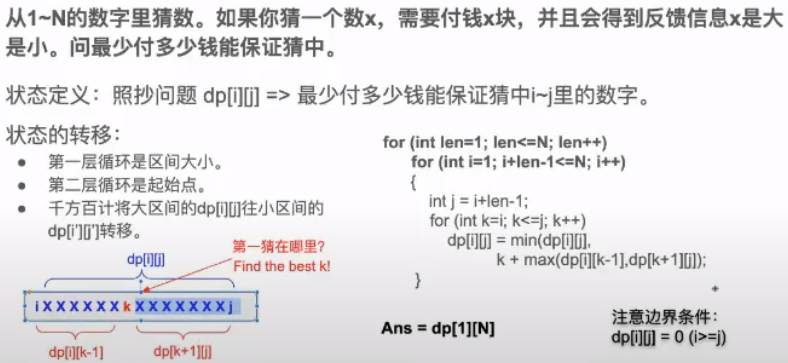
\includegraphics[width=.9\linewidth]{./pic/guessNumber.png}

\begin{minted}[fontsize=\scriptsize,linenos=false]{csharp}
private int dfs(int l, int r) {
    if (dp[l][r] > 0) return dp[l][r];
    if (l == r) return dp[l][r] = 0;
    if (l == r-1) return dp[l][r] = Math.min(l, r);
    int min = Integer.MAX_VALUE;
    for (int i = l; i <= r; i++) 
        min = Math.min(min, i + Math.max((i == r ? i : dfs(i+1, r)), (i == l ? i : dfs(l, i-1))));
    return dp[l][r] = min;
}
int [][] dp;
public int getMoneyAmount(int n) {
    dp = new int[n+1][n+1];
    return dfs(1, n);
}
\end{minted}
\subsection{1478. Allocate Mailboxes - Hard}
\label{sec-1-4-37}
Given the array houses and an integer k. where houses[i] is the location of the ith house along a street, your task is to allocate k mailboxes in the street.

Return the minimum total distance between each house and its nearest mailbox.

The answer is guaranteed to fit in a 32-bit signed integer.

解题思路分析:

对于如何安排邮箱位置,看到很多文章说应放在中位数的位置上,比如一共有1,2,3,4这4间房屋,不论房屋间的距离是多少,如果只有一个邮箱的话,放在房间2处(3也可以)最为合理。这个说法虽然正确,但实际上并不恰当。我们简单的讨论一下这个问题:
\begin{minted}[fontsize=\scriptsize,linenos=false]{csharp}
1.当只有1栋房屋, 1个邮箱时, 显然将邮箱放在房屋处最为合理, 这时邮箱与房屋的距离为0。
2.当有2栋房屋, 1个邮箱时, 比如房屋1在坐标0处, 房屋2在坐标10处, 此时如果将邮箱放在坐标0的话, 它与两栋房屋的距离和为10。
  放在坐标10的情况下距离和也为10。另外我们可以看出, 不论邮箱放在两栋房屋之间的任意位置上, 它与房屋的距离和都是10。因此
  通过此例可得出, 中位数的说法虽然正确, 但并不全面, 不过这不影响本题解题, 对于本题, 我们统一将邮箱安排在房屋位置上是为
  了方便计算, 因此才得出中位数的说法(本例房屋1和2都可以看做是中位数)。
3.当有3栋房屋, 1个邮箱时, 此时通过上面的例子可知, 对于两侧的房子, 将邮筒放在他们之间的任何位置对于结果没有任何影响, 距
  离和都是两栋房子间的距离。但邮箱的位置会对中间的房子产生影响, 因此, 将其放置在中间房子的坐标上最为合理, 这样邮箱与中
  间房屋的距离为0, 可使得全局总距离最小。而中间的房屋正是3个房屋的中位数。
4.当有4栋房屋, 1个邮箱时, 与上例同理, 对于两侧的房子, 将邮筒放在他们之间的任何位置对于结果没有任何影响, 因此邮箱可以考
  虑放在中间两个房屋的任何一个位置上。另外对于中间两个房屋, 不论邮箱放置在其任何一个位置上, 对于总距离都不会产生影响
 (这相当于第2条)。
\end{minted}

因此我们可以得出结论,当有N栋房屋,1个邮箱时,我们将邮箱放在房屋下标的中位数上最为合理。那么,如果有多个邮箱时该怎么办?其实也不难,本题最终可以理解为,我们将一个房屋数组分割为K个子数组(k为邮筒个数),每一个子数组中放置一个邮筒,求最优分割方式。这就变为了经典的动态规划DP问题,对于DP问题我习惯采用递归加记忆数组的方式,本题我们也采用递归方式讲解。

首先建立一个递归函数,参数为当前子区间开始位置index,以及剩余未分配邮筒个数k。起始时,子区间开始位置为下标0,邮筒个数为题目给定的整数k。递归时,当前子区间的开始坐标是参数index,结束坐标范围理论上可以是当前index到数组末尾为止,不过这里有一处可以优化,即要保证剩下的k-1个邮筒都能分配出去的话,还需要至少k-1个子区间,也就是说除了当前子区间外还至少需要k-1个房屋,因此当前子区间的结束坐标范围应该是当前index到length-k为止。我们从index循环至length-k,分别作为当前子区间的结束位置end。并通过中位数方式求出当前子区间[index, end]放置邮筒后的距离和(后文会给出方法)。然后将end加一作为下一个子区间的开始位置,同时k值减去一作为参数传入递归子问题中继续求解。递归函数的返回值加上当前子区间的距离和即是选择当前子区间范围后的一个结果sum。循环完所有当前子区间的结束位置end之后,所有sum中的最小值即是最优方案,也是本层递归的返回值。

接下来再为递归加上一个记忆数组。记忆数组相当于动态规划中使用到的DP数组。由于递归函数中存在2个变量,因此我们需要使用一个2维数组来描述该递归函数,并记录它的返回值。

最后,上文中提到需要求解子区间内放置一个邮筒后所有房屋与邮筒的距离和。这个问题没有太好的方式,只能暴力累加每个房屋与中位数房屋所在位置的距离。为了提高效率,我们可以事先计算好所有区间(排列组合)内放置一个邮筒时的距离和,方便递归中使用,也避免重复运算。这里可能有人会提出质疑,既然递归方法中已经使用了记忆数组,目的就是防止重复计算,这里为什么还担心重复计算距离和呢?原因很简单,记忆数组是二维数组,即在两个条件都满足的情况下才会使用记忆数组中的数据,比如我们计算过以下标5作为子区间起点,并且当前还剩2个油桶的递归函数返回值为x,即memo\footnote{DEFINITION NOT FOUND.}\textsuperscript{,}\,\footnotemark[3]{}=x,再次遇到相同问题时我们可以直接返回x。但是遇到memo\footnotemark[5]{}\textsuperscript{,}\,\footnotemark[2]{}或者memo\footnotemark[5]{}\textsuperscript{,}\,\footnotemark[4]{}时,我们尚未做出过计算,同样还会进入到递归函数内部,如果没有事前计算好下标5到end(end取值范围是5到length-k)的距离和的话,还要重复计算一遍。

对于上述问题,还有一个更好的优化方式即再建立一个保存距离和的记忆数组,计算一个距离和记录一个,方便下次使用。

\begin{minted}[fontsize=\scriptsize,linenos=false]{csharp}
private int getDist(int [] arr, int i, int j) { // 求区间start到end间放置邮筒后的距离和 i: left, j: right
    if (dist[i][j] > 0) return dist[i][j];
    int m = i + (j-i)/2, v = arr[m], sum = 0;
    for (int k = i; k <= j; k++) 
        sum += Math.abs(arr[k] - v);
    return dist[i][j] = sum;
}
private int dfs(int [] arr, int idx, int k) {  // idx: 待分割大子区间的起始坐标;k: 待分割成的子区间的个数 
    if (idx == n || idx == n-k) return 0;
    if (dp[idx][k] > 0) return dp[idx][k];
    if (k == 1) return dp[idx][k] = getDist(arr, idx, n-1);
    int res = Integer.MAX_VALUE;
    for (int i = idx; i < n-(k-1); i++) 
        res = Math.min(res, getDist(arr, idx, i) + dfs(arr, i+1, k-1));
    return dp[idx][k] = res;
}
int [][] dp;
int [][] dist; // 这也是一种记忆数组优化
int n;
public int minDistance(int [] houses, int k) {
    n = houses.length;
    dist = new int [n][n];
    dp = new int [n][k+1];
    Arrays.sort(houses);
    return dfs(houses, 0, k);
}
\end{minted}
\begin{enumerate}
\item 解题思路与分析: 动态规划
\label{sec-1-4-37-1}
\begin{itemize}
\item 复杂度分析
\end{itemize}

时间复杂度:O(n\^{}2k),其中 nn 是数组 houses 的长度。在预处理部分,需要的时间为 O(n\^{}2);在动态规划部分,我们需要 O(nk)O(nk) 的时间枚举每个状态 f[i][j],并使用O(n) 的时间枚举进行状态转移,相乘即可得到总时间复杂度。

空间复杂度:O(n\^{}2 + nk), 即为存储 cost 以及动态规划的状态需要的空间。

\begin{minted}[fontsize=\scriptsize,linenos=false]{csharp}
public int minDistance(int[] h, int k) {
    int n = h.length;
    Arrays.sort(h);
    int [][] medsum = new int[n][n];
    for (int i = n - 2; i >= 0; --i) 
        for (int j = i + 1; j < n; ++j) 
            medsum[i][j] = medsum[i + 1][j - 1] + h[j] - h[i];
    int [][] f = new int[n][k + 1];
    for (int i = 0; i < n; ++i) 
        Arrays.fill(f[i], Integer.MAX_VALUE / 2);
    for (int i = 0; i < n; ++i) {
        f[i][1] = medsum[0][i];
        for (int j = 2; j <= k && j <= i + 1; ++j)
            for (int x = 0; x < i; x++) 
                f[i][j] = Math.min(f[i][j], f[x][j-1] + medsum[x+1][i]);
    }
    return f[n - 1][k];
}
\end{minted}
\end{enumerate}

\subsection{1477. Find Two Non-overlapping Sub-arrays Each With Target Sum}
\label{sec-1-4-38}
Given an array of integers arr and an integer target.
You have to find two non-overlapping sub-arrays of arr each with a sum equal target. There can be multiple answers so you have to find an answer where the sum of the lengths of the two sub-arrays is minimum.
Return the minimum sum of the lengths of the two required sub-arrays, or return -1 if you cannot find such two sub-arrays.
\begin{minted}[fontsize=\scriptsize,linenos=false]{csharp}
// 找出数组中等于target的最小非重叠区间的长度,用dp[i]表示当前i以及i之前的满足条件的最小区间长度,状态更新规则为
//     dp[i]=min(dp[i-1],i-j+1) if sum[j,i]=target
//     答案更新规则
//     res=min(res,dp[j−1]+i−j+1)
public int minSumOfLengths(int[] arr, int target) {
    int n = arr.length;
    int [] dp = new int [n];
    Arrays.fill(dp, Integer.MAX_VALUE);
    int cur = 0, s = 0;
    int res = Integer.MAX_VALUE, minLen = Integer.MAX_VALUE;
    for (int i = 0; i < n; i++) {
        cur += arr[i];
        while (cur > target) {
            cur -= arr[s];
            s += 1;
        }
        if (cur == target) {
            int curLen = i - s + 1;
            if (s > 0 && dp[s-1] != Integer.MAX_VALUE) 
                res = Math.min(res, curLen + dp[s-1]);
            minLen = Math.min(minLen, curLen);
        }
        dp[i] = minLen;
    }
    return res == Integer.MAX_VALUE ? -1 : res;
}
\end{minted}

\subsection{1771. Maximize Palindrome Length From Subsequences}
\label{sec-1-4-39}
You are given two strings, word1 and word2. You want to construct a string in the following manner:
Choose some non-empty subsequence subsequence1 from word1.
Choose some non-empty subsequence subsequence2 from word2.
Concatenate the subsequences: subsequence1 + subsequence2, to make the string.
Return the length of the longest palindrome that can be constructed in the described manner. If no palindromes can be constructed, return 0.
A subsequence of a string s is a string that can be made by deleting some (possibly none) characters from s without changing the order of the remaining characters.
A palindrome is a string that reads the same forward as well as backward.
\begin{minted}[fontsize=\scriptsize,linenos=false]{csharp}
public int longestPalindrome(String ss, String tt) { // 比较喜欢2维dp,比较直接直观
    int m = ss.length(), n = m + tt.length(), ans = 0;
    char [] s = (ss + tt).toCharArray(); // 先求这个联接合并字条串的最长回文子序列
    int [][] dp = new int [n][n];
    for (int i = n-2; i >= 0; i--) {
        dp[i][i] = 1;
        for (int j = i+1; j < n; j++) 
            if (s[i] == s[j]) {
                dp[i][j] = dp[i+1][j-1] + 2;
                if (i < m && j >= m) // 确认来自于两个不同的字条串
                    ans = Math.max(ans, dp[i][j]);
            } else dp[i][j] = Math.max(dp[i+1][j], dp[i][j-1]);
    }
    return ans;
}
\end{minted}
\begin{itemize}
\item 下面是降了一维空间的
\end{itemize}
\begin{minted}[fontsize=\scriptsize,linenos=false]{csharp}
public int longestPalindrome(String ss, String tt) {
    int m = ss.length(), n = m + tt.length(), ans = 0;
    char [] s = (ss + tt).toCharArray(); // 先求这个联接合并字条串的最长回文子序列
    int [] dp = new int[n];
    Arrays.fill(dp, 1);
    int max = 0;
    for (int i = n - 1; i >= 0; i--) {
        int curMax = 0;
        for (int j = i + 1; j < n; j++) {
            int mem = dp[j]; // remember prev dp[j] val
            // curMax = Math.max(curMax, dp[j]);  // bug: curMax 不可以提前更新
            if (s[i] == s[j]) {
                dp[j] = curMax + 2; // 要用更新前的值
                if (i < m && j >= m)
                    max = Math.max(max, dp[j]);
            }
            curMax = Math.max(mem, curMax);
        }
    }
    return max;
}
\end{minted}

\subsection{486. Predict the Winner}
\label{sec-1-4-40}
You are given an integer array nums. Two players are playing a game with this array: player 1 and player 2.
Player 1 and player 2 take turns, with player 1 starting first. Both players start the game with a score of 0. At each turn, the player takes one of the numbers from either end of the array (i.e., nums\footnotemark[1]{} or nums[nums.length - 1]) which reduces the size of the array by 1. The player adds the chosen number to their score. The game ends when there are no more elements in the array.
Return true if Player 1 can win the game. If the scores of both players are equal, then player 1 is still the winner, and you should also return true. You may assume that both players are playing optimally.

博弈类题目,使用minMax思想,使自己分数最大化,对手分数尽量小,递归自顶向下求解。

该题不使用备忘机制同样能通过测试例,只不过耗时相对较长,单纯的比较取数后两players的分数差即可:Math.max(nums[l] - getScore(nums, l + 1, r), nums[r] - getScore(nums, l, r - 1));

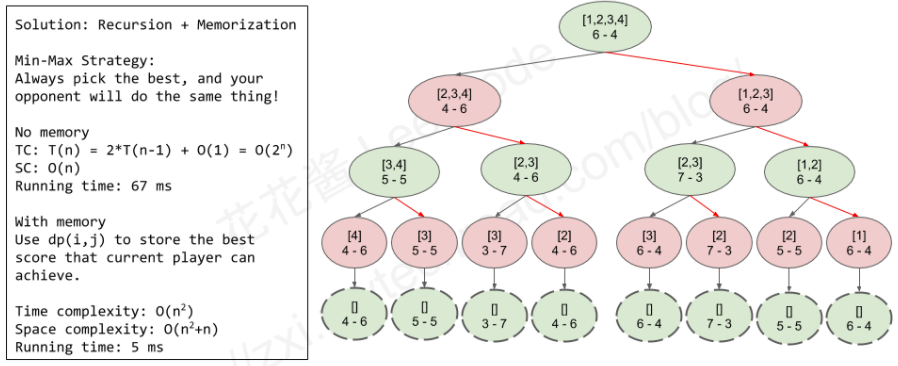
\includegraphics[width=.9\linewidth]{./pic/predictWinner.png}

\begin{minted}[fontsize=\scriptsize,linenos=false]{csharp}
private int helper( int [] arr, int i, int j) {
    if (i == j) return arr[i];
    else return Math.max(arr[i] - helper(arr, i+1, j), arr[j] - helper(arr, i, j-1));
}
public boolean PredictTheWinner(int[] nums) {
    int n = nums.length;
    if (n == 1) return true;
    return helper(nums, 0, n-1) >= 0;
}
\end{minted}

\subsection{1896. Minimum Cost to Change the Final Value of Expression - Hard}
\label{sec-1-4-41}
You are given a valid boolean expression as a string expression consisting of the characters '1','0','\&' (bitwise AND operator),'|' (bitwise OR operator),'(', and ')'.

For example, "()1|1" and "(1)\&()" are not valid while "1", "(((1))|(0))", and "1|(0\&(1))" are valid expressions.
Return the minimum cost to change the final value of the expression.

For example, if expression = "1|1|(0\&0)\&1", its value is 1|1|(0\&0)\&1 = 1|1|0\&1 = 1|0\&1 = 1\&1 = 1. We want to apply operations so that the new expression evaluates to 0.
The cost of changing the final value of an expression is the number of operations performed on the expression. The types of operations are described as follows:

Turn a '1' into a '0'.
Turn a '0' into a '1'.
Turn a '\&' into a '|'.
Turn a '|' into a '\&'.
Note: '\&' does not take precedence over '|' in the order of calculation. Evaluate parentheses first, then in left-to-right order.
\begin{minted}[fontsize=\scriptsize,linenos=false]{csharp}
private int [] getMinOperations(int va, int vb, int ca, int cb, char sign) {
    if (sign == '&') {
        if (va == 1 && vb == 1)      // 1&1, 将其中一个1反转为0
            return new int [] {1, Math.min(ca, cb)};
        else if (va == 0 && vb == 0) // 0&0, 将其中一个0反转为1,并将&反转为|
            return new int [] {0, Math.min(ca, cb) + 1};
        else return new int [] {0, 1}; // 1&0, 将&反转为|
    } else {
        if (va == 1 && vb == 1)        // 1|1,将其中一个1反转为0,并将|反转为&
            return new int [] {1, Math.min(ca, cb) + 1};
        else if (va == 0 && vb == 0)   // 0|0,将其中一个0反转为1
            return new int [] {0, Math.min(ca, cb)};
        else return new int [] {1, 1}; // 1|0,将|反转为&
    }
}
public int minOperationsToFlip(String expression) {
    Stack<Integer> res = new Stack<>();
    Stack<Character> sgn = new Stack<>();
    Stack<Integer> cnt = new Stack<>();
    for (char c : expression.toCharArray()) {
        if (c == '(' || c == '&' || c == '|') {
            sgn.push(c);
            continue;
        } else if (c == ')') sgn.pop();
        else {
            res.push((int)(c - '0'));
            cnt.push(1);
        }
        if (res.size() > 1 && sgn.peek() != '(') {
            int [] loc = getMinOperations(res.pop(), res.pop(), cnt.pop(), cnt.pop(), sgn.pop());
            res.push(loc[0]); // expr results
            cnt.push(loc[1]); // min operations
        }
    }
    return cnt.peek();
}
\end{minted}

\subsection{823. Binary Trees With Factors}
\label{sec-1-4-42}
Given an array of unique integers, arr, where each integer arr[i] is strictly greater than 1.
We make a binary tree using these integers, and each number may be used for any number of times. Each non-leaf node's value should be equal to the product of the values of its children.
Return the number of binary trees we can make. The answer may be too large so return the answer modulo 109 + 7.
\begin{minted}[fontsize=\scriptsize,linenos=false]{csharp}
public int numFactoredBinaryTrees(int[] arr) {
    int n = arr.length;
    Arrays.sort(arr);
    Map<Integer, Long> dp = new HashMap<>();
    int mod = 1_000_000_007;
    long res = 0;
    long max = 0;
    for (int i = 0; i < n; i++) {
        dp.put(arr[i], 1l);
        for (int j = 0; j < i; j++) {
            if (arr[i] % arr[j] == 0 && dp.containsKey(arr[i]/arr[j])) {
                max = dp.get(arr[i]) + dp.get(arr[j]) * dp.get(arr[i]/arr[j]);
                dp.put(arr[i], max % mod);
            }
        }
        res += dp.get(arr[i]);
        res %= mod;
    }
    return (int)(res % mod);
}
\end{minted}

\subsection{907. Sum of Subarray Minimums}
\label{sec-1-4-43}
Given an array of integers arr, find the sum of min(b), where b ranges over every (contiguous) subarray of arr. Since the answer may be large, return the answer modulo 109 + 7.
\begin{minted}[fontsize=\scriptsize,linenos=false]{csharp}
public int sumSubarrayMins(int[] arr) {
    int n = arr.length;
    // for each A[i], find k <= i <= j, so that A[i] is the min from [k,j]
    // sum += A[i] * (i-k+1) * (j-i+1)
    // so we need to find the next min to the right and to the left
    //这个过程可以简化为使用一个栈。对于被某个数从栈中弹出的数而言,它右侧第一个比它小的数就是这个数。所以我们可以对所有被弹出的数得到左侧的区间范围和右侧的区间范围。我觉得这是一种非常聪明的做法。 这个栈我看得稀里糊涂,再想一下
public int sumSubarrayMins(int[] a) { // 以每一个数为最小值找出左右边界。累加和
    int mod = (int)1e9 + 7;
    int n = a.length;
    int [] l = new int [n]; // 以每个当前数为最小值的左右最长边界
    int [] r = new int [n];
    ArrayDeque<Integer> s = new ArrayDeque<>();
    for (int i = 0; i < n; i++) {
        while (!s.isEmpty() && a[i] <= a[s.peek()]) // bug: a[i] < a[s.peek()]
            r[s.pop()] = i-1;
        s.push(i);
    }
    while (!s.isEmpty()) r[s.pop()] = n-1;
    for (int i = n-1; i >= 0; i--) {
        while (!s.isEmpty() && a[i] < a[s.peek()])
            l[s.pop()] = i+1;
        s.push(i);
    }
    while (!s.isEmpty()) 
        l[s.pop()] = 0;
    long sum = 0;
    long lcnt = 0, rcnt = 0;
    for (int i = 0; i < n; i++) {
        lcnt = i - l[i] + 1;
        rcnt = r[i] - i + 1;
        sum += a[i] * lcnt * rcnt;
        sum %= mod;
    }
    return (int)sum;
}
\end{minted}
\begin{enumerate}
\item 解题思路与分析
\label{sec-1-4-43-1}

思路是单调栈。开一个单调递增栈,里面存A AA中的数的下标,并且要保持下标对应的A AA的值单调递增。

遍历A AA,当遍历到A [ i ] A[i]A[i]的时候,如果栈不空并且栈顶t tt对应的值A [ t ] > A [ i ],那么我们就知道了A [ t ]作为最小值的最长的那个区间的左右端点,

先pop掉A [ t ] ,如果栈空了,说明左端点可以取到0 ,否则取栈顶加1(因为栈顶是A [ t ]左边第一个小于等于它的数的下标),而A [ i ] 是A [ t ]右边第一个小于它的数,所以右端点可以取到i − 1。

设左端点取l右端点取r,则以A [ t ]为最小值的区间的数量就是( t − l + 1 ) ( r − t + 1 ) 这么多,所以答案只需要累加一下A [ t ] × ( t − l + 1 ) ( r − t + 1 )即可。

\begin{minted}[fontsize=\scriptsize,linenos=false]{csharp}
public int sumSubarrayMins(int[] a) { // 将上面的三次遍历three passes变为一次遍历求结果
    int mod = (int)1e9 + 7;
    Deque<Integer> s = new ArrayDeque<>();
    long res = 0;
    for (int i = 0; i < a.length; i++) {
        while (!s.isEmpty() && a[i] < a[s.peek()]) { // 对于pop()出来的每一个数,计算出以它为最小值的左右边界,并累加和
            int pos = s.pop();                       // l和r是a[pos]左右数的选择数
            long l = pos - (s.isEmpty() ? -1 : s.peek()), r = i - pos;
            res += (l * r % mod) * a[pos] % mod;
            res %= mod;
        }
        s.push(i);
    }
    while (!s.isEmpty()) {
        int pos = s.pop();
        long l = pos - (s.isEmpty() ? -1 : s.peek()), r = a.length - pos;
        res += (l * r % mod) * a[pos] % mod;
        res %= mod;
    }
    return (int) res;
}
\end{minted}
\begin{itemize}
\item 上面的写法是包装出来的方法,用原始函数来写,效率狠好
\end{itemize}
\begin{minted}[fontsize=\scriptsize,linenos=false]{csharp}
private int MOD = (int)(1e9 + 7);
public int sumSubarrayMins(int[] arr) {
    int n = arr.length;
    Deque<Integer> dk = new LinkedList<>(); // 单调递增栈, 效率狠好!
    long res = 0;
    for (int i = 0; i < n; i++) {
        while (!dk.isEmpty() && arr[dk.peekLast()] > arr[i]) {
            int pkIdx = dk.pollLast();
            int stIdx;
            if (dk.isEmpty()) stIdx = -1;
            else stIdx = dk.peekLast();
            res += (long)arr[pkIdx] * (long)(i - pkIdx) * (long)(pkIdx - stIdx);
        }
        dk.offerLast(i);
    }
    while (!dk.isEmpty()) {
        int pkIdx = dk.pollLast();
        int stIdx;
        if (dk.isEmpty()) stIdx = -1;
        else stIdx = dk.peekLast();
        res += (long)arr[pkIdx] * (long)(n - pkIdx) * (long)(pkIdx - stIdx);
    }
    return (int)(res % MOD);
}
\end{minted}
\begin{itemize}
\item 找到的效率最高的写法
\end{itemize}
\begin{minted}[fontsize=\scriptsize,linenos=false]{csharp}
public int sumSubarrayMins(int[] arr) {
    int sum = 0;
    int mod = (int) 1e9 + 7;
    int curStVal = 0;
    Deque<int[]> s = new ArrayDeque<>(); // int [] {value, count}
    for (int i = 0; i < arr.length; i++) {
        int curCnt = 1;
        int curVal = arr[i];
        while (!s.isEmpty() && s.peek()[0] >= curVal) {
            int[] popped = s.pop();
            curStVal -= popped[1] * popped[0];
            curCnt += popped[1]; // assign all previous count to current
        }
        s.push(new int[]{curVal, curCnt});
        curStVal += curVal * curCnt;
        sum = (sum + curStVal) % mod;
    }
    return sum;
}
\end{minted}
\item 解题思路与分析: 另一种解法吧
\label{sec-1-4-43-2}
\begin{minted}[fontsize=\scriptsize,linenos=false]{csharp}
int mod = 1_000_000_007;
public int sumSubarrayMins(int[] arr) {
    int n = arr.length;
    long [] left = new long[n];
    long [] right = new long[n];
    long sum = 0;
    long cnt = 0;
    int j = 0;
    for (int i = 0; i < n; i++) { // 计算左边比自身大的数的个数
        cnt = 1;
        j = i-1;
        while (j >= 0 && arr[j] >= arr[i]) {
            cnt += left[j];
            j -= left[j];
        }
        left[i] = cnt;
    }
    // 就是因为计算了两个方向,所以对于数组里面有相同元素的情况下,需要特别考虑一下。
    //     不能重复计算, 也不能漏掉,
    //     具体就是一个方向的时候用<=, 另外一个方向的时候用<。 这个在做的时候也bug了。
    for (int i = n-1; i >= 0; i--) { // 计算右边比自身大的数的个数
        cnt = 1;
        j = i+1;
        while (j < n && arr[j] > arr[i]) {
            cnt += right[j];
            j += right[j];
        }
        right [i] = cnt;
    }
    for (int i = 0; i < n; i++) 
        sum += arr[i] * left[i] * right[i];
    return (int) (sum % mod);
}
\end{minted}
\end{enumerate}

\subsection{689. Maximum Sum of 3 Non-Overlapping Subarrays}
\label{sec-1-4-44}
Given an integer array nums and an integer k, find three non-overlapping subarrays of length k with maximum sum and return them.
Return the result as a list of indices representing the starting position of each interval (0-indexed). If there are multiple answers, return the lexicographically smallest one.
\begin{minted}[fontsize=\scriptsize,linenos=false]{csharp}
public int[] maxSumOfThreeSubarrays(int[] nums, int k) {
    int n = nums.length;
    int [] pre = new int [n+1];
    for (int i = 1; i <= n; i++) 
        pre[i] = pre[i-1] + nums[i-1];
    // left[i]表示在区间[0, i]范围内长度为k且和最大的子数组的起始位置
    // right[i]表示在区间[i, n - 1]范围内长度为k且和最大的子数组的起始位置
    int [] left = new int [n];
    int [] right = new int [n];
    int [] res = new int [3];
    Arrays.fill(right, n-k);
    for (int i = k, total = pre[k]-pre[0]; i < n; i++) {
        if (pre[i+1] - pre[i+1-k] > total) {
            left[i]= i+1-k;
            total = pre[i+1] - pre[i+1-k];
        } else left[i] = left[i-1];
    }
    for (int i = n-1-k, total = pre[n]-pre[n-k]; i >= 0; i--) {
        if (pre[i+k] - pre[i] >= total) {
            right[i] = i;
            total = pre[i+k] - pre[i];
        } else right[i] = right[i+1];
    }
    int max = Integer.MIN_VALUE;
    for (int i = k; i <= n-2*k; i++) {
        int l = left[i-1];
        int r = right[i+k];
        int total = (pre[i+k]-pre[i]) + (pre[k+l]-pre[l]) + (pre[r+k] - pre[r]);
        if (max < total) {
            max = total;
            res = new int [] {l, i, r};
        }
    }
    return res;
}
\end{minted}

\subsection{363. Max Sum of Rectangle No Larger Than K}
\label{sec-1-4-45}
Given an m x n matrix matrix and an integer k, return the max sum of a rectangle in the matrix such that its sum is no larger than k.
It is guaranteed that there will be a rectangle with a sum no larger than k.
\begin{enumerate}
\item 解题思路与分析: prefix sum在二维矩阵上的应用
\label{sec-1-4-45-1}

一维数组prefix sum在二维矩阵上的应用,考虑先降一下维度

\begin{minted}[fontsize=\scriptsize,linenos=false]{csharp}
// 把二维数组按行或列拆成多个一维数组,然后利用一维数组的累加和来找符合要求的数字,
// 这里用了 lower _ bound 来加快的搜索速度,也可以使用二分搜索法来替代。
public int maxSumSubmatrix(int[][] mat, int target) {
    int x = mat.length, y = mat[0].length, ans = Integer.MIN_VALUE;
    boolean flag = x <= y;
    int m = Math.min(x, y), n = Math.max(x, y);
    int [] sum = new int [n]; // 定义一维大的数组
    TreeSet<Integer> ts = new TreeSet<>();
    for (int i = 0; i < m; i++) { // 找从第 i 行开始一直到第 0 行这 i+1 行的可能组成的矩形长度
        Arrays.fill(sum, 0);
        for (int j = i; j >= 0; j--) { // 遍历行: 行的和的累加是通过每列列的和的累加sum数组的值来实现的
            ts.clear();
            ts.add(0);
            int cur = 0;
// 因为要满足 ( sum-set 中的元素) <=target,
// 而且 sum-set 中的元素的值要尽可能的大,sum - target <= setElement(要set中的元素,尽可能地小)
// 所以也就是在求大于等于 sum-target 中满足条件的元素的最小的一个
// 正好 TreeSet 中提供了这个方法 ceil() ,可以很方便的找出这个元素: 返回大于或等于e的最小元素;如果没有这样的元素,则返回null
            for (int k = 0; k < n; k++) { // 遍历列: 原始矩阵的行的和,或者是列的和,比较长的大的那一维的和
                if (flag) sum[k] += mat[j][k];
                else sum[k] += mat[k][j];
                cur += sum[k];
                Integer tmp = ts.ceiling(cur - target);
                if (tmp != null) ans = Math.max(ans, cur - tmp);
                ts.add(cur);
            }
        }
    }
    return ans;
}
+END_SRC
- 再稍微简洁一点儿的代码
#+BEGIN_SRC csharp
public int maxSumSubmatrix(int[][] mat, int target) { // 这么再看一下,就清清楚楚地啦
    int m = mat.length, n = mat[0].length, ans = Integer.MIN_VALUE;
    int M = Math.min(m, n), N = Math.max(m, n);
    for (int i = 0; i < M; i++) {
        int [] sum = new int [N];
        for (int j = i; j < M; j++) {
            TreeSet<Integer> ts = new TreeSet<>();
            int cur = 0;
            for (int k = 0; k < N; k++) {
                sum[k] += m > n ? mat[k][j] : mat[j][k];
                cur += sum[k];
                if (cur <= target) ans = Math.max(ans, cur);
                Integer tmp = ts.ceiling(cur - target);
                if (tmp != null) ans = Math.max(ans, cur - tmp);
                ts.add(cur);
            }
        }
    }
    return ans;
}
\end{minted}
\item 解题思路与分析: 暴力+优化
\label{sec-1-4-45-2}

这道题给了我们一个二维数组,让求和不超过的K的最大子矩形,那么首先可以考虑使用 brute force 来解,就是遍历所有的子矩形,然后计算其和跟K比较,找出不超过K的最大值即可。就算是暴力搜索,也可以使用优化的算法,比如建立累加和,参见之前那道题 Range Sum Query 2D - Immutable,可以快速求出任何一个区间和,下面的方法就是这样的,当遍历到 (i, j) 时,计算 sum(i, j),表示矩形 (0, 0) 到 (i, j) 的和,然后遍历这个矩形中所有的子矩形,计算其和跟K相比,这样既可遍历到原矩形的所有子矩形,参见代码如下:

\begin{minted}[fontsize=\scriptsize,linenos=false]{csharp}
public int maxSumSubmatrix(int[][] mat, int k) {
    int m = mat.length;
    int n = mat[0].length;
    if (m == 1 && n == 1) return mat[0][0];
    int [][] pre = new int [m][n];
    int res = Integer.MIN_VALUE;
    for (int i = 0; i < m; i++) {
        for (int j = 0; j < n; j++) {
            int t = mat[i][j];
            if (i > 0) t += pre[i-1][j];
            if (j > 0) t += pre[i][j-1];
            if (i > 0 && j > 0) t -= pre[i-1][j-1];
            pre[i][j] = t;
            for (int r = 0; r <= i; r++) {
                for (int c = 0; c <= j; c++) {
                    int d = pre[i][j];
                    if (r > 0) d -= pre[r-1][j];
                    if (c > 0) d -= pre[i][c-1];
                    if (r > 0 && c > 0) d += pre[r-1][c-1];
                    if (d <= k) res = Math.max(res, d);
                }
            }
        }
    }
    return res;
}
\end{minted}
\end{enumerate}

\subsection{805. Split Array With Same Average}
\label{sec-1-4-46}
You are given an integer array nums.
You should move each element of nums into one of the two arrays A and B such that A and B are non-empty, and average(A) == average(B).
Return true if it is possible to achieve that and false otherwise.
Note that for an array arr, average(arr) is the sum of all the elements of arr over the length of arr.
\begin{minted}[fontsize=\scriptsize,linenos=false]{csharp}
public boolean splitArraySameAverage(int[] nums) {
    int n = nums.length;
    int m = n / 2;
    int sum = Arrays.stream(nums).sum();
    boolean poss = false;
    for (int i = 1; i <= m; i++) 
        if (sum * i % n == 0) {
            poss = true;
            break;
        }
    if (!poss) return false;
    List<Set<Integer>> ls = new ArrayList<>();
    for (int i = 0; i <= m; i++) 
        ls.add(new HashSet<Integer>());
    ls.get(0).add(0);    // 这种构建子序列和的方法,要学习一下
    for (int v : nums)  // for each element in A, we try to add it to sums[i] by joining sums[i - 1]
        for (int i = m; i >= 1; i--) 
            for (int t : ls.get(i-1)) 
                ls.get(i).add(t + v);
    for (int i = 1; i <= m; i++) {
        if (sum * i % n == 0 && ls.get(i).contains(sum * i / n))
            return true;
    }
    return false;
}
\end{minted}

\subsection{1884. Egg Drop With 2 Eggs and N Floors - Medium}
\label{sec-1-4-47}
You are given two identical eggs and you have access to a building with n floors labeled from 1 to n.

You know that there exists a floor f where 0 <= f <= n such that any egg dropped at a floor higher than f will break, and any egg dropped at or below floor f will not break.

In each move, you may take an unbroken egg and drop it from any floor x (where 1 <= x <= n). If the egg breaks, you can no longer use it. However, if the egg does not break, you may reuse it in future moves.

Return the minimum number of moves that you need to determine with certainty what the value of f is.
\begin{minted}[fontsize=\scriptsize,linenos=false]{csharp}
    // 思路: https://zhuanlan.zhihu.com/p/41257286 可以借这个思路理解一下
    // DP[i][j]表示用i个鸡蛋,j层楼的情况下最坏情况下所需扔鸡蛋的最少数目。
    // 可知初始条件为:
    // DP[1][0] = 0; DP[2][0] = 0;
    // DP[1][1] = 1; DP[2][1] = 1;
    // DP[1][i] = i; //i = 1 … n
    // 对于DP[2][i], i = 2 … n的情况,我们可以这样考虑:
    //     遍历j=2…i,求DP[2][j],分两种情况:
    //     如果第1个鸡蛋在第j-1层摔破了,则我们在第j层只需摔第2个鸡蛋一次即可,此时总摔鸡蛋数为DP[1][j-1]+1。
    //     注意上面的1是因为第j层需要摔第2个鸡蛋1次。为什么DP[1][j-1]不能写成1呢?因为第1个鸡蛋在第j-1层摔破了,我们不能肯定在第1,2,…,j-2层不会破,所以要用DP[1][j-1]。
    //     如果第1个鸡蛋在第j-1层没有摔破,则我们在第j到i层有2个鸡蛋可以摔,此时退化到DP[2][i-j]的情况。该种情形下总共扔1+DP[2][i-j]。那个1就是表示第1个鸡蛋在第j-1层扔了1次。这里我们为什么只考虑用1,而不用考虑DP[1][j-1]呢?因为如果第j-1层没有摔破,第1,2,…,j-2层也就不用考虑了。
    //     因为是求最坏情况下的数目,所以DP[2][j]=1 + max(DP[1][j-1]+1, DP[2][i-j])。
    //     而我们是要求所有最坏情况下的最少数目,所以DP[2][j]=min(1 + max(DP[1][j-1]+1, DP[2][i-j]))。i = 2…n, j = 2…i。
public int twoEggDrop(int n) { // 1 + 2 + 3 + ... + x >= n ==> get x
    if (n <= 1) return n;
    int [][] dp = new int [3][n+1]; // DP[i][j]表示用i个鸡蛋,j层楼的情况下最坏情况下所需扔鸡蛋的最少数目。
    for (int i = 0; i < 3; i++) 
        Arrays.fill(dp[i], Integer.MAX_VALUE);
    dp[1][0] = 0;
    dp[1][1] = 1;
    dp[2][0] = 0;
    dp[2][1] = 1;
    for (int i = 1; i <= n; i++) dp[1][i] = i;
    for (int i = 2; i <= n; i++) 
        for (int j = 2; j <= i; j++) 
            dp[2][i] = Math.min(dp[2][i], 1 + Math.max(dp[1][j-1], dp[2][i-j])); // 1: 这个鸡蛋在j-i层扔了一次,要统计入结果
    return dp[2][n];
}
public int twoEggDrop(int n) { // 1 + 2 + 3 + ... + x >= n ==> get x
    if (n <= 2) return n;
    return (int)(Math.ceil((-1 + Math.sqrt((long)n * 8 + 1)) / 2.0));
}
\end{minted}
\subsection{887. Super Egg Drop - Hard}
\label{sec-1-4-48}
You are given k identical eggs and you have access to a building with n floors labeled from 1 to n.

You know that there exists a floor f where 0 <= f <= n such that any egg dropped at a floor higher than f will break, and any egg dropped at or below floor f will not break.

Each move, you may take an unbroken egg and drop it from any floor x (where 1 <= x <= n). If the egg breaks, you can no longer use it. However, if the egg does not break, you may reuse it in future moves.

Return the minimum number of moves that you need to determine with certainty what the value of f is.
\begin{enumerate}
\item 解题思路与分析
\label{sec-1-4-48-1}
\begin{itemize}
\item \url{https://charlesliuyx.github.io/2018/10/11/\%E3\%80\%90\%E7\%9B\%B4\%E8\%A7\%82\%E7\%AE\%97\%E6\%B3\%95\%E3\%80\%91Egg\%20Puzzle\%20\%E9\%B8\%A1\%E8\%9B\%8B\%E9\%9A\%BE\%E9\%A2\%98/}
\item \url{https://www.shuzhiduo.com/A/D8548M4Q5E/}
\end{itemize}
\item 解题思路与分析
\label{sec-1-4-48-2}
1 <= K <= 100, 
1 <= N <= 10000

这道题说给了我们K个鸡蛋,还有一栋共N层的大楼,说是鸡蛋有个临界点的层数F,高于这个层数扔鸡蛋就会碎,否则就不会,问我们找到这个临界点最小需要多少操作,注意这里的操作只有当前还有没碎的鸡蛋才能进行。这道题是基于经典的扔鸡蛋的问题改编的,原题是有 100 层楼,为了测鸡蛋会碎的临街点,最少可以扔几次?答案是只用扔 14 次就可以测出来了,讲解可以参见[油管上的这个视频](\url{https://www.youtube.com/watch?v=NGtt7GJ1uiM}),这两道题看着很相似,其实是有不同的。这道题限制了鸡蛋的个数K,假设我们只有1个鸡蛋,碎了就不能再用了,这时我们要测 100 楼的临界点的时候,只能一层一层去测,当某层鸡蛋碎了之后,就知道临界点了,所以最坏情况要测 100 次,注意要跟经典题目中扔 14 次要区分出来。那么假如有两个鸡蛋呢,其实需要的次数跟经典题目中的一样,都是 14 次,这是为啥呢?因为在经典题目中,我们是分别间隔 14,13,12,\ldots{},2,1,来扔鸡蛋的,当我们有两个鸡蛋的时候,我们也可以这么扔,第一个鸡蛋仍在 14 楼,若碎了,说明临界点一定在 14 楼以内,可以用第二个鸡蛋去一层一层的测试,所以最多操作 14 次。若第一个鸡蛋没碎,则下一次扔在第 27 楼,假如碎了,说明临界点在 (14,27] 范围内,用第二个鸡蛋去一层一层测,总次数最多 13 次。若第一个鸡蛋还没碎,则继续按照 39, 50, \ldots{}, 95, 99,等层数去测,总次数也只可能越来越少,不会超过 14 次的。但是照这种思路分析的话,博主就不太清楚有3个鸡蛋,在 100 楼测,最少的步骤数,答案是9次,博主不太会分析怎么测的,各位看官大神知道的话一定要告诉博主啊。

其实这道题比较好的解法是用动态规划 Dynamic Programming,因为这里有两个变量,鸡蛋数K和楼层数N,所以就要使用一个二维数组 DP,其中 dp[i][j] 表示有i个鸡蛋,j层楼要测需要的最小操作数。那么我们在任意k层扔鸡蛋的时候就有两种情况(注意这里的k跟鸡蛋总数K没有任何关系,k的范围是 [1, j]):
\begin{minted}[fontsize=\scriptsize,linenos=false]{csharp}
鸡蛋碎掉:接下来就要用 i-1 个鸡蛋来测 k-1 层,所以需要 dp[i-1][k-1] 次操作。
鸡蛋没碎:接下来还可以用i个鸡蛋来测 j-k 层,所以需要 dp[i][j-k] 次操作。
\end{minted}

因为我们每次都要面对最坏的情况,所以在第j层扔,需要 max(dp[i-1][k-1], dp[i][j-k])+1 步,状态转移方程为:

dp[i][j] = min(dp[i][j], max(dp[i - 1][k - 1], dp[i][j - k]) + 1) ( 1 <= k <= j )

\begin{minted}[fontsize=\scriptsize,linenos=false]{csharp}
public int superEggDrop(int k, int n) { // tle:  O(KN^2) 还需要优化一下
    if (k < 1 || n < 1) return 0;
    int [] pre = new int [n+1]; //上一层备忘录,存储鸡蛋数量-1的n层楼条件下的最优化尝试次数
    int [] cur = new int [n+1]; // 当前备忘录,存储当前鸡蛋数量的n层楼条件下的最优化尝试次数
    for (int i = 1; i <= n; i++) // 把备忘录每个元素初始化成最大的尝试次数
        cur[i] = i;
    for (int i = 2; i <= k; i++) {
        pre = cur.clone(); // 当前备忘录拷贝给上一次备忘录,并重新初始化当前备忘录
        for (int j = 1; j <= n; j++) cur[j] = j;
        for (int j = 1; j <= n; j++) // 需要想办法去优化时间复杂度。这种写法里面我们枚举了 [1, j] 范围所有的k值,总时间复杂度为 O(KN^2),
            for (int x = 1; x < j; x++) 
// 扔鸡蛋的楼层从1到m枚举一遍,如果当前算出的尝试次数小于上一次算出的尝试次数,则取代上一次的尝试次数。
// 这里可以打印k的值,从而知道第一个鸡蛋是从第几次扔的。
                cur[j] = Math.min(cur[j], 1 + Math.max(pre[x-1], cur[j-x]));
    }
    return cur[n];
}
\end{minted}

这种写法会超时 Time Limit Exceeded,代码请参见评论区1楼,OJ 对时间卡的还是蛮严格的,所以我们就需要想办法去优化时间复杂度。这种写法里面我们枚举了 [1, j] 范围所有的k值,总时间复杂度为 O(KN\^{}2),若我们仔细观察 dp[i - 1][k - 1] 和 dp[i][j - k],可以发现前者是随着k递增,后者是随着k递减,且每次变化的值最多为1,所以只要存在某个k值使得二者相等,那么就能得到最优解,否则取最相近的两个k值做比较,由于这种单调性,我们可以在 [1, j] 范围内对k进行二分查找,找到第一个使得 dp[i - 1][k - 1] 不小于 dp[i][j - k] 的k值,然后用这个k值去更新 dp[i][j] 即可,这样时间复杂度就减少到了 O(KNlgN),其实也是险过,参见代码如下:

\begin{minted}[fontsize=\scriptsize,linenos=false]{csharp}
// 若我们仔细观察 dp[i - 1][k - 1] 和 dp[i][j - k],可以发现前者是随着k递增,后者是随着k递减,且每次变化的值最多为1,
// 所以只要存在某个k值使得二者相等,那么就能得到最优解,否则取最相近的两个k值做比较,
// 由于这种单调性,我们可以在 [1, j] 范围内对k进行二分查找,找到第一个使得 dp[i - 1][k - 1] 不小于 dp[i][j - k] 的k值,然后用这个k值去更新 dp[i][j] 即可,
// 这样时间复杂度就减少到了 O(KNlgN)
public int superEggDrop(int k, int n) { // O(KNlgN)
    int [][] dp = new int [k+1][n+1];
    for (int i = 1; i <= n; i++) dp[1][i] = i; // 把只有一个鸡蛋的情况初始化为最大值
    for (int i = 2; i <= k; i++) {
        for (int j = 1; j <= n; j++) {
            dp[i][j] = j;
            int l = 1, r = j, m = 0;
            while (l < r) {
                m = (l + r) / 2;
                if (dp[i-1][m-1] < dp[i][j-m]) l = m + 1; // < 左边随m递增,< 右边随m递减,这个性质在这里很重要,所以可以二分查找
                else r = m;
            } // 这里查找的右边界也注意一下
            dp[i][j] = Math.min(dp[i][j], Math.max(dp[i-1][r-1], dp[i][j-r]) + 1); // 用这个鸡蛋测试了一次了
        }
    }
    return dp[k][n];
}
\end{minted}

进一步来想,对于固定的k,dp[i][j-k] 会随着j的增加而增加,最优决策点也会随着j单调递增,所以在每次移动j后,从上一次的最优决策点的位置来继续向后查找最优点即可,这样时间复杂度就优化到了 O(KN),我们使用一个变量s表示当前的j值下的的最优决策点,然后当j值改变了,我们用一个 while 循环,来找到第下一个最优决策点s,使得 dp[i - 1][s - 1] 不小于 dp[i][j - s],参见代码如下:

\begin{minted}[fontsize=\scriptsize,linenos=false]{csharp}
public int superEggDrop(int k, int n) { // O(KN)
    int [][] dp = new int [k+1][n+1];
    for (int i = 1; i <= n; i++) dp[1][i] = i; // 把只有一个鸡蛋的情况初始化为最大值
    for (int i = 2; i <= k; i++) {
        int s = 1; // k
        for (int j = 1; j <= n; j++) { // n
            dp[i][j] = j;
            while (s < j && dp[i-1][s-1] < dp[i][j-s]) s++; // 因为单调性,s一直向右滑动,总共执行n次
            dp[i][j] = Math.min(dp[i][j], Math.max(dp[i-1][s-1], dp[i][j-s]) + 1);
        }
    }
    return dp[k][n];
}
\end{minted}

其实我们还可以进一步优化时间复杂度到 O(KlgN),不过就比较难想到了,需要将问题转化一下,变成已知鸡蛋个数,和操作次数,求最多能测多少层楼的临界点。还是使用动态规划 Dynamic Programming 来做,用一个二维 DP 数组,其中 dp[i][j] 表示当有i次操作,且有j个鸡蛋时能测出的最高的楼层数。再来考虑状态转移方程如何写,由于 dp[i][j] 表示的是在第i次移动且使用第j个鸡蛋测试第 dp[i-1][j-1]+1 层,因为上一个状态是第i-1次移动,且用第j-1个鸡蛋。此时还是有两种情况:

鸡蛋碎掉:说明至少可以测到的不会碎的层数就是 dp[i-1][j-1]。

鸡蛋没碎:那这个鸡蛋可以继续利用,此时我们还可以再向上查找 dp[i-1][j] 层。

那么加上当前层,总共可以通过i次操作和j个鸡蛋查找的层数范围是 [0, dp[i-1][j-1] + dp[i-1][j] + 1],这样就可以得到状态转移方程如下:

dp[i][j] = dp[i - 1][j - 1] + dp[i - 1][j] + 1

当 dp[i][K] 正好小于N的时候,i就是我们要求的最小次数了,参见代码如下:

\begin{minted}[fontsize=\scriptsize,linenos=false]{csharp}
public int superEggDrop(int k, int n) { // O(KlgN): 为什么说这里就是 O(klgN)呢?因为dp[m][k]的增长呈指数级的?
    int [][] dp = new int [n+1][k+1]; // 在第 i 次移动且使用第 j 个鸡蛋测试第 dp[i-1][j-1]+1 层
    int m = 0; // 最小测试次数
    while (dp[m][k] < n) { // 当dp[m][k] == n,退出循环的时候,m就是要求的最小操作次数了
        ++m;
        for (int j = 1; j <= k; j++) 
            dp[m][j] = dp[m-1][j-1] + dp[m-1][j] + 1; // 分上一次测的 第j-1个鸡蛋 碎了 和 没有碎 两种情况来更新当前值
    }
    return m;
}
\end{minted}

我们可以进一步的优化空间,因为当前的操作次数值的更新只跟上一次操作次数有关,所以我们并不需要保存所有的次数,可以使用一个一维数组,其中 dp[i] 表示当前次数下使用i个鸡蛋可以测出的最高楼层。状态转移方程的推导思路还是跟上面一样,参见代码如下:
\begin{minted}[fontsize=\scriptsize,linenos=false]{csharp}
public int superEggDrop(int k, int n) { // O(KlgN): 空间压缩
    int [] dp = new int [k+1]; // dp[i] 表示当前次数下使用 i 个鸡蛋可以测出的最高楼层
    int ans = 0;
    for (; dp[k] < n; ans++) // 压缩代码到一行
        for (int i = k; i >= 1; i--) // 压缩空间后,因为是想要根据上一行[ans-1]时的i-1/i来更新当前结果,需要倒序遍历以免产生脏数据
            dp[i] = dp[i] + dp[i-1] + 1;
    return ans;
}
\end{minted}

下面这种方法就非常的 tricky 了,居然推导出了使用k个鸡蛋,移动x次所能测的最大楼层数的通项公式,推导过程可以参见[这个帖子](\url{https://leetcode.com/problems/super-egg-drop/discuss/181702/Clear-C\%2B\%2B-codeRuntime-0-msO(1)}-spacewith-explation.No-DPWhat-we-need-is-mathematical-thought!),通项公式如下:

f(k,x) = x(x-1)..(x-k)/k! + \ldots{} + x(x-1)(x-2)/3! + x(x-1)/2! + x

这数学功底也太好了吧,有了通向公式后,我们就可以通过二分搜索法 Binary Search 来快速查找满足题目的x。这里其实是博主之前总结贴 [LeetCode Binary Search Summary 二分搜索法小结](\url{http://www.cnblogs.com/grandyang/p/6854825.html}) 中的第四类,用子函数当作判断关系,这里子函数就是用来实现上面的通向公式的,不过要判断,当累加和大于等于N的时候,就要把当的累加和返回,这样相当于进行了剪枝,因为在二分法中只需要知道其跟N的大小关系,并不 care 到底大了多少,这样快速定位x的方法运行速度貌似比上面的 DP 解法要快不少,但是这通项公式尼玛谁能容易的推导出来,只能膜拜叹服了,参见代码如下:

\begin{minted}[fontsize=\scriptsize,linenos=false]{csharp}
public int superEggDrop(int k, int n) { // O(KlgN):数学推导找出了推理公式,速度最快
    int l = 1, r = n;
    while (l < r) { // 寻找右边界
        int m = l + (r - l) / 2;
        if (helper(m, k, n) < n) l = m + 1;
        else r = m;
    }
    return r;
}
int helper(int m, int k, int n) { // 能查找到的最大楼层数
    int ans = 0, r = 1;
    for (int i = 1; i <= k; i++) {
        r *= m - i + 1;
        r /= i;
        ans += r;
        if (ans >= n) break;
    }
    return ans;
}
\end{minted}
\end{enumerate}

\subsection{1981. Minimize the Difference Between Target and Chosen Elements}
\label{sec-1-4-49}
You are given an m x n integer matrix mat and an integer target.
Choose one integer from each row in the matrix such that the absolute difference between target and the sum of the chosen elements is minimized.
Return the minimum absolute difference.
The absolute difference between two numbers a and b is the absolute value of a - b.
\begin{minted}[fontsize=\scriptsize,linenos=false]{csharp}
// DP + BitSet : 这里面有个小问题需要挑出来
// 使用一个DP数组存下当前行和之前行每行选一个数可能构成的和,
// 在本题中,可以使用BitSet(简介)来存储之前行可以组成的和(由于所有数的最大值为70,而行数最大也为70,故BitSet最大的位数即为4900)。
// 对于当前行,遍历BitSet已经set过的位(即代表之前行可能组成的和),然后加上当前数,set新的和
// 最后遍历BitSet,求出当前位与target的最小值
public int minimizeTheDifference(int[][] mat, int target) {
    int m = mat.length;
    int n = mat[0].length;
    BitSet sum = new BitSet(); // 遍历每一行,存下当前行和之前行可能组成的和
    for (int i = 0; i < n; i++) // 初始时存下第一行
        sum.set(mat[0][i]);
    for (int i = 1; i < m; i++) {
        BitSet newSum = new BitSet(); // 用来存新的和
        for (int j = 0; j < n; j++) {
            // 注意:要遍历BitSet中的真实位,请使用以下循环:previousSetBit()方法 用于查找在指定的起始索引上或之前是否存在任何真位
            // for (int i = bs.length(); (i = bs.previousSetBit(i-1)) >= 0; ) {
            //     // operate on index i here
            // }
            for (int k = sum.length(); (k = sum.previousSetBit(k-1)) >= 0; ) {
                newSum.set(k+mat[i][j]);
            }
        }
        sum = newSum;
    }
    int ans = 4900;
    for (int k = sum.length(); (k = sum.previousSetBit(k-1)) >= 0;) {
        int diff = Math.abs(k - target);
        ans = Math.min(ans, diff);
    }
    return ans;
}
public int minimizeTheDifference(int[][] mat, int target) {
    int m = mat.length;
    int n = mat[0].length;
    int diff = Integer.MAX_VALUE, limit = 4900;
    int [] dp = new int[limit];
    for (int i = 0; i < n; i++) // 相当于是手工实现java BitSet
        dp[mat[0][i]] = 1;
    for (int i = 1; i < m; i++) {
        int [] tmp = new int [limit];
        for (int v = limit-1; v >= 0; v--) {
            if (dp[v] == 0) continue;
            for (int j = 0; j < n; j++) {
                if (v + mat[i][j] < limit)
                    tmp[v+mat[i][j]] = 1;
            }
        }
        System.arraycopy(tmp, 0, dp, 0, dp.length);
    }
    for (int i = 0; i < limit; i++) 
        if (dp[i] > 0) diff = Math.min(diff, Math.abs(i-target));
    return diff;  // min difference
}
\end{minted}

\subsection{805. Split Array With Same Average}
\label{sec-1-4-50}
You are given an integer array nums.
You should move each element of nums into one of the two arrays A and B such that A and B are non-empty, and average(A) == average(B).
Return true if it is possible to achieve that and false otherwise.
Note that for an array arr, average(arr) is the sum of all the elements of arr over the length of arr.
\begin{minted}[fontsize=\scriptsize,linenos=false]{csharp}
    //     1)如果一个长度为n的数组可以被划分为A和B两个数组,我们假设A的长度小于B并且A的大小是k,那么:total_sum / n == A_sum / k == B_sum / (n - k),其中1 <= k <= n / 2。那么可以知道:A_sum = total_sum * k / n。由于A_sum一定是个整数,所以我们可以推导出total_sum * k % n == 0,那就是说,对于特定的total_sum和n而言,符合条件的k不会太多。这样我们在第一步中就首先验证是否存在符合条件的k,如果不存在就可以提前返回false。
    //     2)如果经过第一步的验证,发现确实有符合条件的k,那么我们在第二步中,就试图产生k个子元素的所有组合,并且计算他们的和。这里的思路就有点类似于背包问题了,vector<unordered_set<int>> sums,其中sums[i][j]表示A[0, i]这个子数组中的任意j个元素的所有可能和。可以得到递推公式是:sums[i][j] = sums[i - 1][j] "join" (sums[i][j - 1] + A[i]),其中等式右边的第一项表示这j个元素中不包含A[i],而第二项表示这j个元素包含A[i]。这样就可以采用动态规划的思路得到sums[n - 1][k]了(1 <= k <= n / 2)。
    // 3)有了sums[n - 1][k],我们就检查sums[n - 1][k]中是否包含(total_sum * k / n)。一旦发现符合条件的k,就返回true,否则就返回false。
    // 在递推公式中我们发现,sums[i][j]仅仅和sums[i - 1][j],sums[i][j - 1]有关,所以可以进一步将空间复杂度从O(n^2*M)降低到O(n*M),其中M是n中的所有元素的组合数(可能高达O(2^n))。时间复杂度为O(n^3*M)。
public boolean splitArraySameAverage(int[] nums) {
    int n = nums.length;
    int m = n / 2;
    int sum = Arrays.stream(nums).sum();
    boolean poss = false;
    for (int i = 1; i <= m; i++) {
        if (sum * i % n == 0) {
            poss = true;
            break;
        }
    }
    if (!poss) return false;
    List<Set<Integer>> ls = new ArrayList<>();
    for (int i = 0; i <= m; i++) 
        ls.add(new HashSet<Integer>());
    ls.get(0).add(0);    // 这种构建子序列和的方法,要学习一下
    for (int v : nums) { // for each element in A, we try to add it to sums[i] by joining sums[i - 1]
        for (int i = m; i >= 1; i--) {
            for (int t : ls.get(i-1)) {
                ls.get(i).add(t + v);
            }
        }
    }
    // System.out.println("ls.size(): " + ls.size());
    // for (int z = 0; z < ls.size(); ++z) {
    //     for (Integer x : ls.get(z))
    //         System.out.print(x + ", ");
    //     System.out.print("\n");
    //     System.out.print("\n ");
    // }
    for (int i = 1; i <= m; i++) {
        if (sum * i % n == 0 && ls.get(i).contains(sum * i / n))
            return true;
    }
    return false;
}
private boolean helper(int [] arr, int curSum, int cur, int start) {
    if (cur == 0) return curSum == 0;
    if (arr[start] > curSum / cur) return false;
    for (int i = start; i < arr.length - cur + 1; i++) {
        if (i > start && arr[i] == arr[i-1]) continue;
        if (helper(arr, curSum - arr[i], cur-1, i+1)) return true;
    }
    return false;
}
public boolean splitArraySameAverage(int[] nums) {
    int n = nums.length;
    int m = n / 2;
    int sum = Arrays.stream(nums).sum();
    boolean poss = false;
    for (int i = 1; i <= m; i++) {
        if (sum * i % n == 0) {
            poss = true;
            break;
        }
    }
    if (!poss) return false;
    Arrays.sort(nums);
    for (int i = 1; i <= m; i++) 
        if (sum * i % n == 0 && helper(nums, sum * i / n, i, 0)) return true;
    return false;
}
bool splitArraySameAverage(vector<int>& A) {  // https://www.cnblogs.com/grandyang/p/10285531.html
    int n = A.size(), m = n / 2, sum = accumulate(A.begin(), A.end(), 0);
    bool possible = false;
    for (int i = 1; i <= m && !possible; ++i) {
        if (sum * i % n == 0) possible = true;
    }
    if (!possible) return false;
    bitset<300001> bits[m + 1] = {1};
    for (int num : A) {
        for (int i = m; i >= 1; --i) {
            bits[i] |= bits[i - 1] << num;
        }
    }
    for (int i = 1; i <= m; ++i) {
        if (sum * i % n == 0 && bits[i][sum * i / n]) return true;
    }
    return false;
}
\end{minted}

\subsection{801. Minimum Swaps To Make Sequences Increasing - Hard}
\label{sec-1-4-51}
You are given two integer arrays of the same length nums1 and nums2. In one operation, you are allowed to swap nums1[i] with nums2[i].

For example, if nums1 = [1,2,3,8], and nums2 = [5,6,7,4], you can swap the element at i = 3 to obtain nums1 = [1,2,3,4] and nums2 = [5,6,7,8].
Return the minimum number of needed operations to make nums1 and nums2 strictly increasing. The test cases are generated so that the given input always makes it possible.

An array arr is strictly increasing if and only if arr\footnotemark[1]{} < arr\footnotemark[2]{} < arr\footnotemark[3]{} < \ldots{} < arr[arr.length - 1].
\begin{minted}[fontsize=\scriptsize,linenos=false]{csharp}
// 设 dp[0][i] 表示不交换 A[i] 和 B[i] 在下标 i 的交换次数
// 设 dp[1][i] 表示交换 A[i] 和 B[i] 在下标 i 的交换次数
// 可以看到交换与否只取决与前一个状态, 可以将空间复杂度压缩到 O(1)
//     时间复杂度为 O(n), 空间复杂度为 O(1)
public int minSwap(int[] a, int[] b) {
    int n = a.length;
    int [][] dp = new int [2][n];
    for (int [] row : dp) 
        Arrays.fill(row, Integer.MAX_VALUE);
    dp[0][0] = 0;
    dp[1][0] = 1;
    for (int i = 1; i < n; i++) {
        if (a[i] > a[i-1] && b[i] > b[i-1]) {
            dp[0][i] = Math.min(dp[0][i], dp[0][i-1]);    // 不需要交换不用增加交换次数
            dp[1][i] = Math.min(dp[1][i], dp[1][i-1] + 1);// 如果要交换前一个也必须交换才能满足递增的条件
        }
        if (a[i] > b[i-1] && b[i] > a[i-1]) {
            dp[0][i] = Math.min(dp[0][i], dp[1][i-1]);    // 表示 i - 1 位置发生交换  
            dp[1][i] = Math.min(dp[1][i], dp[0][i-1] + 1);// 表示在 i - 1 不换的基础上, i 发生了交换 
        }
    }
    return Math.min(dp[0][n-1], dp[1][n-1]);
}
\end{minted}
\subsection{837. New 21 Game - Medium}
\label{sec-1-4-52}
Alice plays the following game, loosely based on the card game "21".

Alice starts with 0 points and draws numbers while she has less than k points. During each draw, she gains an integer number of points randomly from the range [1, maxPts], where maxPts is an integer. Each draw is independent and the outcomes have equal probabilities.

Alice stops drawing numbers when she gets k or more points.

Return the probability that Alice has n or fewer points.

Answers within 10-5 of the actual answer are considered accepted.
\begin{minted}[fontsize=\scriptsize,linenos=false]{csharp}
// When the draws sum up to K, it stops, calculate the possibility K<=sum<=N.
//     Think about one step earlier, sum = K-1, game is not ended and draw largest card W.
//     K-1+W is the maximum sum could get when game is ended. If it is <= N, then for sure the possiblity when games end ans sum <= N is 1.
//     Because the maximum is still <= 1.
//     Otherwise calculate the possibility sum between K and N.
//     Let dp[i] denotes the possibility of that when game ends sum up to i.
//     i is a number could be got equally from i - m and draws value m card.
//     Then dp[i] should be sum of dp[i-W] + dp[i-W+1] + ... + dp[i-1], devided by W.
//     We only need to care about previous W value sum, accumlate winSum, reduce the possibility out of range.
//     Time Complexity: O(N).
//     Space: O(N).
public double new21Game(int n, int k, int w) { // k : threshold
    if (k == 0 || n >= (k + w)) return 1.0;
    if (k > n) return 0;
    double [] dp = new double [n+1];
    dp[0] = 1.0;
    double winSum = 1;
    double res = 0;
    for (int i = 1; i <= n; i++) {
        dp[i] = winSum / w;
        if (i < k) winSum += dp[i];
        else res += dp[i];
        if (i >= w) winSum -= dp[i-w];
    }
    return res;
}
\end{minted}
\subsection{1105. Filling Bookcase Shelves - Medium}
\label{sec-1-4-53}
You are given an array books where books[i] = [thicknessi, heighti] indicates the thickness and height of the ith book. You are also given an integer shelfWidth.

We want to place these books in order onto bookcase shelves that have a total width shelfWidth.

We choose some of the books to place on this shelf such that the sum of their thickness is less than or equal to shelfWidth, then build another level of the shelf of the bookcase so that the total height of the bookcase has increased by the maximum height of the books we just put down. We repeat this process until there are no more books to place.

Note that at each step of the above process, the order of the books we place is the same order as the given sequence of books.

For example, if we have an ordered list of 5 books, we might place the first and second book onto the first shelf, the third book on the second shelf, and the fourth and fifth book on the last shelf.
Return the minimum possible height that the total bookshelf can be after placing shelves in this manner.
\begin{minted}[fontsize=\scriptsize,linenos=false]{csharp}
// 求摆放前i本书需要的最小高度,首先需要求摆放前i-1书需要的最小高度,以此类推,最初需要计算的是摆放第0本书需要的最小高度,也就是0。
// 根据前i-1本书求前i书需要的最小高度的思路是:
// 尝试①将第i本书放在前i-1本书的下面
// 以及②将前i-1本书的最后几本和第i本书放在同一层两种方案,看哪种方案高度更小就用哪种方案,依次求出摆放前1,…,n本书需要的最小高度。
public int minHeightShelves(int[][] books, int shelfWidth) {
    int [] dp = new int [books.length + 1];
    for (int i = 1; i < dp.length; i++) { // 依次求摆放前i本书的最小高度
        int width = books[i-1][0];
        int height = books[i-1][1];
        dp[i] = dp[i-1] + height;
        // 将前i - 1本书从第i - 1本开始放在与i同一层,直到这一层摆满或者所有的书都摆好
        for (int j = i-1; j > 0 && width + books[j-1][0] <= shelfWidth; j--) {
            height = Math.max(height, books[j-1][1]); // 每层的高度由最高的那本书决定
            width += books[j-1][0];
            dp[i] = Math.min(dp[i], dp[j-1] + height);// 选择高度最小的方法
        }
    }            
    return dp[books.length];
}
\end{minted}
\begin{itemize}
\item 后来又出的bug
\end{itemize}
\begin{minted}[fontsize=\scriptsize,linenos=false]{csharp}
public int minHeightShelves(int [][] b, int w) { 
    int n = b.length, curLayerWidth = 0, max = 0;
    int [] dp = new int [n+1];
    Arrays.fill(dp, n+1);
    dp[0] = 0;
    for (int i = 1; i <= n; i++) {   // 依次求摆放前i本书的最小高度
        dp[i] = dp[i-1] + b[i-1][1]; // 初始化为最大值:单列一行,再看之前的行有没有空隙可以放入之前的层?
        curLayerWidth = b[i-1][0];
         max = b[i-1][1];
        for (int j = i-1; j > 0 && curLayerWidth + b[j-1][0] <= w; j--) { // 将前i - 1本书从第i - 1本开始放在与i同一层,直到这一层摆满或者所有的书都摆好
            curLayerWidth += b[j-1][0];
            max = Math.max(max, b[j-1][1]);
            // dp[i] = Math.min(dp[i], dp[j] + max);  // bug: dp[j] + max 是从第j本开始,包括第j本,这与之后的书放到最后一层所能形成的最小高度
            dp[i] = Math.min(dp[i], dp[j - 1] + max); // 所以,是用j之前所开成的最小高度,dp[j-1]加上最后一层所能形成的最小高度
        }
    }
    return dp[n];
}
\end{minted}
\subsection{790. Domino and Tromino Tiling}
\label{sec-1-4-54}
You have two types of tiles: a 2 x 1 domino shape and a tromino shape. You may rotate these shapes.

Given an integer n, return the number of ways to tile an 2 x n board. Since the answer may be very large, return it modulo 109 + 7.

In a tiling, every square must be covered by a tile. Two tilings are different if and only if there are two 4-directionally adjacent cells on the board such that exactly one of the tilings has both squares occupied by a tile.
\begin{enumerate}
\item 解题思路与分析
\label{sec-1-4-54-1}

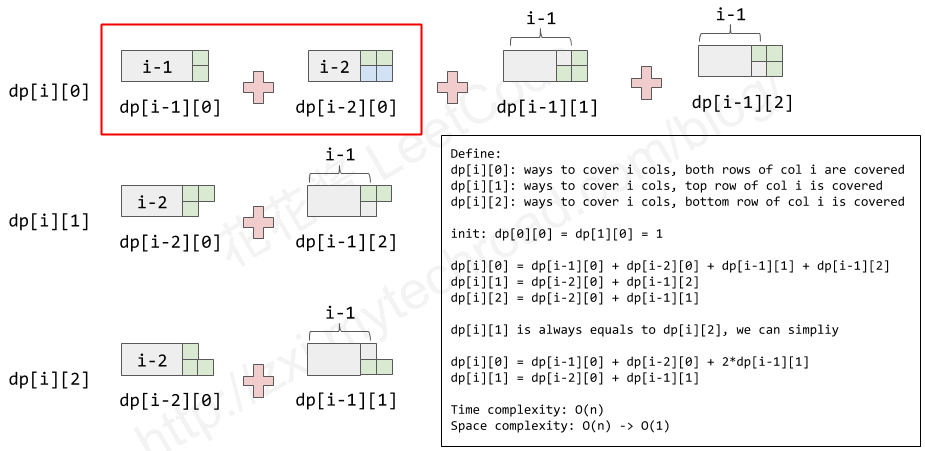
\includegraphics[width=.9\linewidth]{./pic/790.png}

\begin{minted}[fontsize=\scriptsize,linenos=false]{csharp}
public int numTilings(int n) {
    int mod = (int)1e9 + 7;
    int [][] dp = new int [n+1][2];
    dp[0][0] = 1;
    dp[1][0] = 1;
    for (int i = 2; i <= n; i++) {
        dp[i][0] = (int)((dp[i-1][0] + dp[i-2][0]) % mod + (2 * dp[i-1][1]) % mod) % mod;
        dp[i][1] = (int)(dp[i-2][0] + dp[i-1][1]) % mod;
    }
    return dp[n][0];
}
\end{minted}
\end{enumerate}
\subsection{1997. First Day Where You Have Been in All the Rooms - Medium}
\label{sec-1-4-55}
There are n rooms you need to visit, labeled from 0 to n - 1. Each day is labeled, starting from 0. You will go in and visit one room a day.

Initially on day 0, you visit room 0. The order you visit the rooms for the coming days is determined by the following rules and a given 0-indexed array nextVisit of length n:

Assuming that on a day, you visit room i,
if you have been in room i an odd number of times (including the current visit), on the next day you will visit a room with a lower or equal room number specified by nextVisit[i] where 0 <= nextVisit[i] <= i;
if you have been in room i an even number of times (including the current visit), on the next day you will visit room (i + 1) mod n.
Return the label of the first day where you have been in all the rooms. It can be shown that such a day exists. Since the answer may be very large, return it modulo 109 + 7.
\begin{minted}[fontsize=\scriptsize,linenos=false]{csharp}
public int firstDayBeenInAllRooms(int [] nextVisit) {
    int n = nextVisit.length, mod = (int)1e9 + 7;
    long [] dp = new long [n];
    dp[0] = 0;
    for (int i = 1; i < n; i++) 
        dp[i] = (2 * dp[i-1] % mod + mod - dp[nextVisit[i-1]] + 2) % mod;
    return (int)dp[n-1];
}
\end{minted}

\subsection{943. Find the Shortest Superstring - Hard}
\label{sec-1-4-56}
Given an array of strings words, return the smallest string that contains each string in words as a substring. If there are multiple valid strings of the smallest length, return any of them.

You may assume that no string in words is a substring of another string in words.
\begin{itemize}
\item 深搜 + 记忆数组 + 裁枝
\end{itemize}
\begin{minted}[fontsize=\scriptsize,linenos=false]{csharp}
public String shortestSuperstring(String [] sa) { // 回塑: 暴搜+剪枝,但回塑仍然是最慢的方法
    n = sa.length;
    max = new int [n][n];
    for (int i = 0; i < n; i++) 
        for (int j = 0; j < n; j++) {
            if (i == j) continue;
            for (int k = Math.min(sa[i].length(), sa[j].length()); k >= 1; k--) // 不想遍历所有,找到一个有效最优解,就剪枝中断
                if (sa[i].substring(sa[i].length()-k).equals(sa[j].substring(0, k))) {
                    max[i][j] = k; // sa[i] 的尾 与 sa[j]的头的 最长公共后前缀 长度
                    break;
                }
        }                
    dp = new int [1 << n][n];
    ans = new int [n]; // 最终答案: 最小长度的字符串下标位置
    vis = new boolean [n];
    dfs(new int [n], 0, 0, 0);
    String s = sa[ans[0]];
    for (int i = 1; i < n; i++) { // 当前字符串的前缀已经被上一个字符串的后缀cover了,所以只取后没被覆盖住的后半部分
        int cmnLen = max[ans[i-1]][ans[i]];
        s += sa[ans[i]].substring(cmnLen);
    }
    return s;
}
int [][] dp;
int [][] max; // max common length between two strings
boolean [] vis;
int n, maxLen = Integer.MIN_VALUE; // BUG: has to be initialized 
int [] ans;
private void dfs(int [] a, int idx, int sum, int state) {
    if (idx == n) {
        if (sum > maxLen) {
            maxLen = sum;
            // ans = Arrays.copyOf(a, n);
            ans = a.clone(); // 效果一样
        }
        return ;
    }
    for (int i = 0; i < n; i++) {
        if (vis[i]) continue;
        int mask = state | (1 << i);
        int curLen = sum + (idx == 0 ? 0 : max[a[idx-1]][i]);
        if (dp[mask][i] > 0 && dp[mask][i] >= curLen) continue; // == 的情况可以剪枝,因为dp[][]本来就是记忆着各路径状态下的全局最优解,不能更优就剪掉
        vis[i] = true;
        a[idx] = i;
        dp[mask][i] = curLen; // BUG: 需要这一行记忆化,加速搜索与剪枝,重中之重不可记忆, otherwise tle !!!
        dfs(a, idx+1, curLen, mask);
        vis[i] = false;
    }
}
\end{minted}
\begin{itemize}
\item 动态规划
\end{itemize}
\begin{minted}[fontsize=\scriptsize,linenos=false]{csharp}
public String shortestSuperstring(String[] s) {
    int n = s.length;
    String [][] dp = new String [1 << n][n]; // 这个dp的设计还比较新颖奇特:
    int [][] max = new int [n][n];
    for (int i = 0; i < n; i++) 
        for (int j = 0; j < n; j++) {
            if (i == j) continue;
            for (int k = Math.min(s[i].length(), s[j].length()); k >= 1; k--) 
                 if (s[i].substring(s[i].length()-k).equals(s[j].substring(0, k))) {
                    max[i][j] = k;
                    break;
                }
        }
    for (int i = 0; i < n; i++) dp[1 << i][i] = s[i]; // 初始化:每个字符串与自己的最长公共后前缀串就是它本身
    for (int r = 1; r < 1 << n; r++) 
        for (int i = 0; i < n; i++) {
            if (((r >> i) & 1) == 0) continue;
            for (int j = 0; j < n; j++) {
                if (i == j || (((r >> j) & 1) == 0)) continue; // 保证状态r是包含了字符串i和j的有效state
                String cur = dp[r ^ (1 << j)][i] + s[j].substring(max[i][j]);
                if (dp[r][j] == null || dp[r][j].length() > cur.length()) // dp[i][j]: 这里比较字符串的长度操作起来就比较复杂一点儿
                    dp[r][j] = cur;
            }
        }
     int r = (1 << n) - 1;
    String ans = dp[r][0];
    for (int i = 1; i < n; i++) 
        if (dp[r][i].length() < ans.length()) ans = dp[r][i];
    return ans;
}
\end{minted}
\begin{enumerate}
\item 解题思路与分析
\label{sec-1-4-56-1}

我们的算法包括三个部分:

预先计算出所有的 overlap(A[i], A[j]);

使用动态规划计算出所有的 dp(mask, i),并记录每个状态从哪个状态转移得来,记为 parent;

通过 parent 还原这个字符串。

\begin{minted}[fontsize=\scriptsize,linenos=false]{csharp}
public String shortestSuperstring(String[] A) {
    int N = A.length;
    int[][] overlaps = new int[N][N];
    for (int i = 0; i < N; ++i)
        for (int j = 0; j < N; ++j) if (i != j) {
                int m = Math.min(A[i].length(), A[j].length());
                for (int k = m; k >= 0; --k)
                    if (A[i].endsWith(A[j].substring(0, k))) {
                        overlaps[i][j] = k;
                        break;
                    }
            }
    int[][] dp = new int[1<<N][N]; // dp[mask][i] = most overlap with mask, ending with ith element
    int[][] parent = new int[1<<N][N];
    for (int mask = 0; mask < (1<<N); ++mask) {
        Arrays.fill(parent[mask], -1);
        for (int bit = 0; bit < N; ++bit) if (((mask >> bit) & 1) > 0) {
                // Let's try to find dp[mask][bit].  Previously, we had a collection of items represented by pmask.
                int pmask = mask ^ (1 << bit);
                if (pmask == 0) continue;
                for (int i = 0; i < N; ++i) if (((pmask >> i) & 1) > 0) {
                        // For each bit i in pmask, calculate the value if we ended with word i, then added word 'bit'.
                        int val = dp[pmask][i] + overlaps[i][bit];
                        if (val > dp[mask][bit]) {
                            dp[mask][bit] = val;
                            parent[mask][bit] = i;
                        }
                    }
            }
    }
    // # Answer will have length sum(len(A[i]) for i) - max(dp[-1])
    // Reconstruct answer, first as a sequence 'perm' representing the indices of each word from left to right.
    int[] perm = new int[N];
    boolean[] vis = new boolean[N];
    int t = 0;
    int mask = (1 << N) - 1;
    // p: the last element of perm (last word written left to right)
    int p = 0;
    for (int j = 0; j < N; ++j)
        if (dp[(1<<N) - 1][j] > dp[(1<<N) - 1][p])
            p = j;
    // Follow parents down backwards path that retains maximum overlap
    while (p != -1) {
        perm[t++] = p;
        vis[p] = true;
        int p2 = parent[mask][p];
        mask ^= 1 << p;
        p = p2;
    }
    // Reverse perm
    for (int i = 0; i < t/2; ++i) {
        int v = perm[i];
        perm[i] = perm[t-1-i];
        perm[t-1-i] = v;
    }
    // Fill in remaining words not yet added
    for (int i = 0; i < N; ++i)
        if (!vis[i]) perm[t++] = i;
    // Reconstruct final answer given perm
    StringBuilder ans = new StringBuilder(A[perm[0]]);
    for (int i = 1; i < N; ++i) {
        int overlap = overlaps[perm[i-1]][perm[i]];
        ans.append(A[perm[i]].substring(overlap));
    }
    return ans.toString();
}
\end{minted}
\end{enumerate}
\subsection{964. Least Operators to Express Number - Hard}
\label{sec-1-4-57}
Given a single positive integer x, we will write an expression of the form x (op1) x (op2) x (op3) x \ldots{} where each operator op1, op2, etc. is either addition, subtraction, multiplication, or division (+, -, *, or /). For example, with x = 3, we might write 3 * 3 / 3 + 3 - 3 which is a value of 3.

When writing such an expression, we adhere to the following conventions:

The division operator (/) returns rational numbers.
There are no parentheses placed anywhere.
We use the usual order of operations: multiplication and division happen before addition and subtraction.
It is not allowed to use the unary negation operator (-). For example, "x - x" is a valid expression as it only uses subtraction, but "-x + x" is not because it uses negation.
We would like to write an expression with the least number of operators such that the expression equals the given target. Return the least number of operators used.

博主看了一会儿,发现没思路就直接放弃了,直奔论坛上找解法。这里直接参考 donggua\_fu 大神的解法吧,首先处理 edge cases,当 x 等于 target 的话,不用加任何运算符,返回0即可。若 x 大于 target,比如 x=5,target=3,我们其实可以迅速的求出运算符的个数,因为5比3大,要凑3就只能先变成1,这里就有两种变法,一种是全部都变成1,然后来凑3,即 5/5 + 5/5 + 5/5,这时的运算符个数是 target * 2 -1,因为加号的个数总是比除号少一个。另一种凑法就是 5 - 5/5 - 5/5,这时候的运算符个数是 (x - target) * 2,此时的加号和除号的个数相同,均为x和 target 的差值。

接下来就要处理 x 小于 target 的情况了,此时由于不知道x到底比 target 小多少,若差距太大的话,肯定不能用加号,所以应该先用乘号来让x变大,直到刚好大于等于 target 停止,并每次增加次数 cnt。若此时 sum 正好等于 target,太幸运了,直接返回 cnt。但通常情况下 sum 会大于 target,此时 sum - target 的差值就需要另行计算了。这里差值跟 target 的大小关系又要分为两种情况来讨论,当 sum - target < target 时,比如 x=5,sum=25,target=15,则 sum - target=10,就是说现在已经乘到了 25,但需要再减去 10,这个差值 10 可以再次调用原函数来计算,此时新的 target 代入 10 即可,记得返回值要加上 cnt。当然之后还是要再计算一下另一种凑的方法,由于 sum 超过了 target,所以回退一个x,变成 sum / x,此时小于 target,那么它们的差值 target - (sum / x) 就可以通过再次调用函数来计算,注意这里加上 cnt 之后还要减去1,因为回退了一个x,少了一个乘号。最终二者的较小值即为所求,记得要加上个1,以为多加了个运算符,参见代码如下:

\begin{minted}[fontsize=\scriptsize,linenos=false]{csharp}
public int leastOpsExpressTarget(int x, int target) {
    if (x == target) return 0;
    if (x > target) return Math.min(target*2-1, (x-target)*2);
    int cnt = 0;
    long sum = x;
    while (sum  < target) {
        sum *= x;
        ++cnt;
    }
    if (sum == target) return cnt;
    int min = Integer.MAX_VALUE, max = Integer.MIN_VALUE;
    // int tmp = sum - target; // -
    if (sum - target < target)
        min = leastOpsExpressTarget(x, (int)(sum - target)) + cnt;
    max = leastOpsExpressTarget(x, (int)(target - (sum / x))) + cnt - 1;
    return Math.min(min, max) + 1; // -
}
\end{minted}
\begin{itemize}
\item 和race car 那道题类似。注意到,符号的添加就是对数字 进行 -x\^{}i 的操作,最后要减到0,k = logx(t),有两种方式,可以先到 t 前面的数字,2\^{}k, 或者 t后面的数字 2\^{}(k+1)。
\end{itemize}
注意,2\^{}k需要的符号是k,最后因为第一个一定可以是正的,省一个符号。

看了花花酱的题解,感觉更像是bfs。cost小的点先扩展。 \textbf{这个再看一下}

\begin{minted}[fontsize=\scriptsize,linenos=false]{cpp}
int leastOpsExpressTarget(int x, int target) {
    priority_queue<pair<int, int>, vector<pair<int, int>>, greater<pair<int, int>>> que;
    unordered_set<int> s;
    que.emplace(0, target);
    while(!que.empty()) {
        int cost = que.top().first;
        int t = que.top().second;
        que.pop();
        if (t == 0) return cost-1;
        if (s.count(t)) continue;
        s.insert(t);
        int k = log(t) / log(x);
        int l = t - pow(x, k);
        que.emplace(cost+(k == 0 ? 2 : k), l);
        int r = pow(x, k+1) - t;
        que.emplace(cost+k+1, r);
    }
    return -1;
}
\end{minted}
\subsection{1955. Count Number of Special Subsequences - Hard 把这些个递推公式记住}
\label{sec-1-4-58}
A sequence is special if it consists of a positive number of 0s, followed by a positive number of 1s, then a positive number of 2s.

For example, [0,1,2] and [0,0,1,1,1,2] are special.
In contrast, [2,1,0], \footnotemark[2]{}, and [0,1,2,0] are not special.
Given an array nums (consisting of only integers 0, 1, and 2), return the number of different subsequences that are special. Since the answer may be very large, return it modulo 109 + 7.

A subsequence of an array is a sequence that can be derived from the array by deleting some or no elements without changing the order of the remaining elements. Two subsequences are different if the set of indices chosen are different.

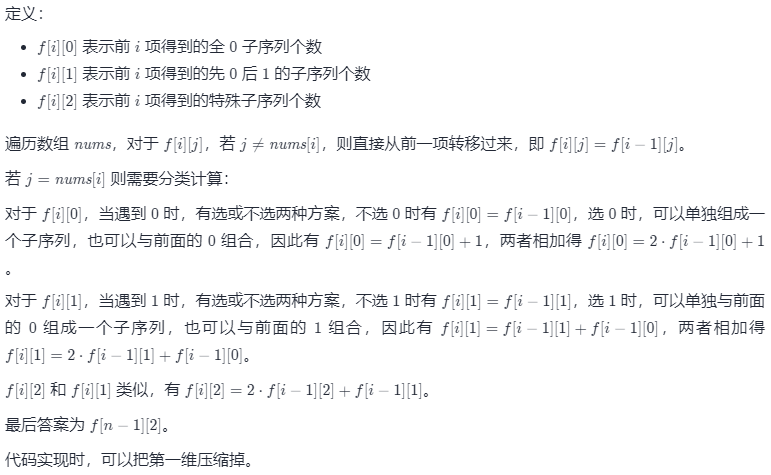
\includegraphics[width=.9\linewidth]{./pic/specialSeq.png}

\begin{minted}[fontsize=\scriptsize,linenos=false]{csharp}
public int countSpecialSubsequences(int[] arr) { // 去找个降维的参考一下
    int mod = (int)1e9 + 7;
    int n = arr.length;
    long [][] dp = new long [n][3];
    for (int i = 0; i < n; i++) 
        for (int j = 0; j < 3; j++) {
            if (arr[i] != j) dp[i][j] = (i == 0 ? 0 : dp[i-1][j]);
            else 
                if (j == 0)
                    dp[i][j] = (i == 0 ? 0 : dp[i-1][j]) * 2 % mod + 1;
                else
                    dp[i][j] = ((i == 0 ? 0 : dp[i-1][j]) * 2 % mod + (i == 0 ? 0 : dp[i-1][j-1])) % mod;
        }
    return (int)dp[n-1][2];
}
\end{minted}

\subsection{446. Arithmetic Slices II - Subsequence - Hard}
\label{sec-1-4-59}
Given an integer array nums, return the number of all the arithmetic subsequences of nums.

A sequence of numbers is called arithmetic if it consists of at least three elements and if the difference between any two consecutive elements is the same.

For example, [1, 3, 5, 7, 9], [7, 7, 7, 7], and [3, -1, -5, -9] are arithmetic sequences.
For example, [1, 1, 2, 5, 7] is not an arithmetic sequence.
A subsequence of an array is a sequence that can be formed by removing some elements (possibly none) of the array.

For example, [2,5,10] is a subsequence of [1,2,1,2,4,1,5,10].
The test cases are generated so that the answer fits in 32-bit integer.
\begin{enumerate}
\item 解题思路与分析
\label{sec-1-4-59-0-1}
这道题是之前那道Arithmetic Slices的延伸,那道题比较简单是因为要求等差数列是连续的,而这道题让我们求是等差数列的子序列,可以跳过某些数字,不一定非得连续,那么难度就加大了,但还是需要用动态规划Dynamic Progrmming来做。

好,既然决定要用DP了,那么首先就要确定dp数组的定义了,刚开始我们可能会考虑使用个一维的dp数组,然后dp[i]定义为范围为[0, i]的子数组中等差数列的个数。定义的很简单,OK,但是基于这种定义的状态转移方程却十分的难想。我们想对于(0, i)之间的任意位置j,如何让 dp[i] 和 dp[j] 产生关联呢?是不是只有 A[i] 和 A[j] 的差值diff,跟A[j]之前等差数列的差值相同,才会有关联,所以差值diff是一个很重要的隐藏信息Hidden Information,我们必须要在dp的定义中考虑进去。所以一维dp数组是罩不住的,必须升维,但是用二维dp数组的话,差值diff那一维的范围又是个问题,数字的范围是整型数,所以差值的范围也很大,为了节省空间,我们建立一个一维数组dp,数组里的元素不是数字,而是放一个HashMap,建立等差数列的差值和当前位置之前差值相同的数字个数之间的映射。我们遍历数组中的所有数字,对于当前遍历到的数字,又从开头遍历到当前数字,计算两个数字之差diff,如果越界了不做任何处理,如果没越界,我们让dp[i]中diff的差值映射自增1,因为此时A[i]前面有相差为diff的A[j],所以映射值要加1。然后我们看dp[j]中是否有diff的映射,如果有的话,说明此时相差为diff的数字至少有三个了,已经能构成题目要求的等差数列了,将dp[j][diff]加入结果res中,然后再更新dp[i][diff],这样等遍历完数组,res即为所求。

我们用题目中给的例子数组 [2,4,6,8,10] 来看,因为2之前没有数字了,所以我们从4开始,遍历前面的数字,是2,二者差值为2,那么在dp\footnotemark[2]{}的HashMap就可以建立 2->1 的映射,表示4之前有1个差值为2的数字,即数字2。那么现在i=2指向6了,遍历前面的数字,第一个数是2,二者相差4,那么在dp\footnotemark[3]{}的HashMap就可以建立 4->1 的映射,第二个数是4,二者相差2,那么先在dp\footnotemark[3]{}的HashMap建立 2->1 的映射,由于dp\footnotemark[2]{}的HashMap中也有差值为2的映射,2->1,那么说明此时至少有三个数字差值相同,即这里的 [2 4 6],我们将dp\footnotemark[2]{}中的映射值加入结果res中,然后当前dp\footnotemark[3]{}中的映射值加上dp\footnotemark[2]{}中的映射值。这应该不难理解,比如当i=3指向数字8时,j=2指向数字6,那么二者差值为2,此时先在dp\footnotemark[4]{}建立 2->1 的映射,由于dp\footnotemark[3]{}中有 2->2 的映射,那么加上数字8其实新增了两个等差数列 [2,4,6,8] 和 [4,6,8],所以结果res加上的值就是 dp[j][diff],即2,并且 dp[i][diff] 也需要加上这个值,才能使得 dp\footnotemark[4]{} 中的映射变为 2->3 ,后面数字10的处理情况也相同,这里就不多赘述了,最终的各个位置的映射关系如下所示:
\begin{minted}[fontsize=\scriptsize,linenos=false]{csharp}
2     4     6     8     10    
     2->1  4->1  6->1  8->1
           2->2  4->1  6->1 
                 2->3  4->2
                       2->4
\end{minted}

最终累计出来的结果是跟上面红色的数字相关,分别对应着如下的等差数列:

\begin{minted}[fontsize=\scriptsize,linenos=false]{csharp}
2->2:[2,4,6]
2->3:[2,4,6,8]    [4,6,8]
4->2:[2,6,10]
2->4:[2,4,6,8,10]    [4,6,8,10]    [6,8,10]
\end{minted}
\begin{itemize}
\item Both time and space complexities are O(n\^{}2)
\end{itemize}

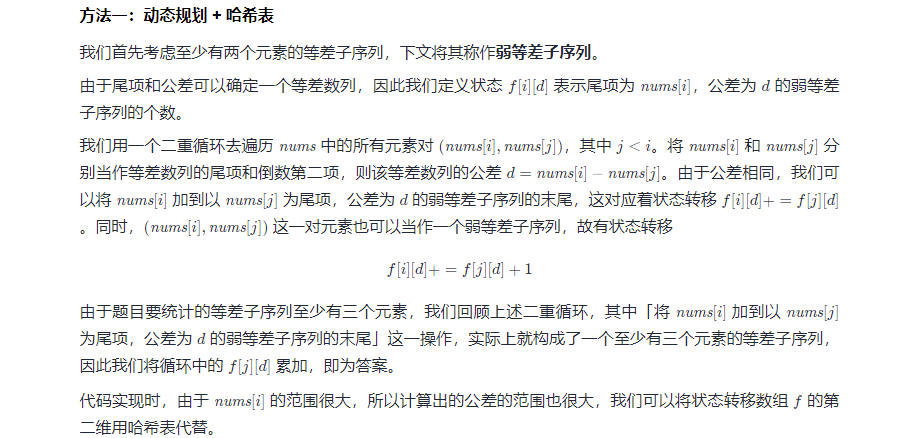
\includegraphics[width=.9\linewidth]{./pic/arithslice.png}

Define the type of the difference as Integer type instead of Long. This is because there is no valid arithmetic subsequence slice that can have difference out of the Integer value range. But we do need a long integer to filter out those invalid cases.

Preallocate the HashMap to avoid reallocation to deal with extreme cases.

Refrain from using lambda expressions inside loops.

\begin{minted}[fontsize=\scriptsize,linenos=false]{csharp}
 public int numberOfArithmeticSlices(int [] a) {
    int n = a.length, ans = 0;
    Map<Integer, Integer> [] dp = new HashMap[n];
    dp[0] = new HashMap<>();
    for (int i = 1; i < n; i++) {
        dp[i] = new HashMap<>();
        for (int j = 0; j < i; j++) {
        // for (int j = i-1; j >= 0; j--) { // BUG: 反向遍历不可以
            long diff = (long)a[i] - a[j];  // bug: (long)a[i]
            if (diff > Integer.MAX_VALUE || diff < Integer.MIN_VALUE) continue;
            int dif = (int)diff;
            dp[i].put(dif, dp[i].getOrDefault(dif, 0) + 1); // bug: 这里加的是1,不是2 // 这里先更新上
            if (dp[j].containsKey(dif)) {
                ans += dp[j].get(dif); // 只自增1(而不是记为2),为的是方便这里统计结果
                dp[i].put(dif, dp[i].get(dif) + dp[j].get(dif));// 再加上之前累积的
            }
        }
    }
    return ans;
}
\end{minted}
\end{enumerate}

\subsection{639. Decode Ways II - Hard}
\label{sec-1-4-60}
A message containing letters from A-Z can be encoded into numbers using the following mapping:

'A' -> "1"
'B' -> "2"
\ldots{}
'Z' -> "26"
To decode an encoded message, all the digits must be grouped then mapped back into letters using the reverse of the mapping above (there may be multiple ways). For example, "11106" can be mapped into:

"AAJF" with the grouping (1 1 10 6)
"KJF" with the grouping (11 10 6)
Note that the grouping (1 11 06) is invalid because "06" cannot be mapped into 'F' since "6" is different from "06".

In addition to the mapping above, an encoded message may contain the '*' character, which can represent any digit from '1' to '9' ('0' is excluded). For example, the encoded message "1*" may represent any of the encoded messages "11", "12", "13", "14", "15", "16", "17", "18", or "19". Decoding "1*" is equivalent to decoding any of the encoded messages it can represent.

Given a string s consisting of digits and '*' characters, return the number of ways to decode it.

Since the answer may be very large, return it modulo 109 + 7.
\begin{enumerate}
\item 解题思路与分析
\label{sec-1-4-60-0-1}
给定一个只含数字的长n nn的字符串s ss,再给定一个对应规则,每个大写字母ch可以对应一个数字ch - 'A' + 1。问该s ss有多少种不同的解码方式。s ss中可能含有'*',这个符号可以对应除了0 00以外的任意一位数。答案模10\^{}9 + 7后返回。

思路是动态规划。设f [ i ] f[i]f[i]是s ss的长i ii的前缀的解码方式数,那么可以按照最后一位(或者两位)是解码成什么字母来分类进行累加。
\begin{minted}[fontsize=\scriptsize,linenos=false]{csharp}
public int numDecodings(String t) {
    int mod = (int)1e9 + 7;
    int n = t.length();
    char [] s = t.toCharArray();
    System.out.println(Arrays.toString(s));
    int [] dp = new int [Math.max(2, n+1)];
    dp[0] = 1;
    dp[1] = s[0] == '*' ? 9 : s[0] == '0' ? 0 : 1;
    for (int i = 2; i <= n; i++) {
        System.out.println("i: " + i);
        for (int j = 1; j <= 26; j++) { // 枚举s的长i前缀的末尾可以解码为哪个大写字母
            char c = s[i-1];
            if (j <= 9) { // 如果是要解码为A到I,那么最后一个数字得单独解码
                if (c == '*' || c == '0' + j)
                    dp[i] += dp[i-1];
            } else {      // 否则最后两个数字得一起解码
                char p = s[i-2];
                int x = j % 10, y = j / 10;
                if ((p == '*' || p == y+ '0') && ((c == '*' && x != 0) || c == x + '0')) 
                    dp[i] += dp[i-2];
            }
            dp[i] %= mod;
        }
    }
    return dp[n];
}
\end{minted}
\item 解题思路与分析
\label{sec-1-4-60-0-2}

定义dp[i]是nums前i个字符可以得到的解码种数,假设之前的字符串是abcx,现在新加入了y,则有以下5种情况:

\begin{minted}[fontsize=\scriptsize,linenos=false]{csharp}
如果x=='0',且y=='0',无法解码,返回0;
如果只有x=='0',则y只能单独放在最后,不能与x合并(不能以0开头),此时有:dp[i] = dp[i-1]
如果只有y=='0',则y不能单独放置,必须与x合并,并且如果合并结果大于26,返回0,否则有:dp[i] = dp[i-2]
如果 xy<=26: 则y可以“单独”放在abcx的每个解码结果之后后,并且如果abcx以x单独结尾,此时可以合并xy作为结尾,而这种解码种数就是abc的解码结果,此时有:dp[i+1] = dp[i] + dp[i-1]
如果 xy>26: 此时x又不能与y合并,y只能单独放在dp[i]的每一种情况的最后,此时有:dp[i+1] = dp[i]
\end{minted}
\begin{minted}[fontsize=\scriptsize,linenos=false]{csharp}
    public int numDecodings(String s) {
        char[] arr = s.toCharArray();
        int[] dp = new int[s.length()+1];
        dp[0] = 1;
        dp[1] = arr[0]=='0'?0:1;
        if(s.length()<=1) return dp[1];
        for(int i=2;i<=s.length();i++){
            int n = (arr[i-2]-'0')*10+(arr[i-1]-'0');
            if(arr[i-1]=='0' && arr[i-2]=='0'){
                return 0;
            }else if(arr[i-2]=='0'){
                dp[i] = dp[i-1];
            }else if(arr[i-1]=='0'){
                if(n>26) return 0;
                dp[i] = dp[i-2];
            }else if(n>26){
                dp[i] = dp[i-1];
            }else{
                dp[i] = dp[i-1]+dp[i-2];
            }
        }
        return dp[dp.length-1];
    }
\end{minted}
\end{enumerate}

\subsection{629. K Inverse Pairs Array - Hard}
\label{sec-1-4-61}
For an integer array nums, an inverse pair is a pair of integers [i, j] where 0 <= i < j < nums.length and nums[i] > nums[j].

Given two integers n and k, return the number of different arrays consist of numbers from 1 to n such that there are exactly k inverse pairs. Since the answer can be huge, return it modulo 109 + 7.
\begin{enumerate}
\item 解题思路与分析
\label{sec-1-4-61-0-1}

比较容易辨别出来是一道DP的题目,但是确实算是比较难的了,下面是参考网上的代码之后我的理解。定义dp[n][k]表示从1到n构成的数中含有k个逆序对的个数,则我们可以推导出dp[n][k]和dp[n - 1][i]之间的递推关系:

如果我们把n放在最后一位,则所有的k个逆序对均来自于前n - 1个数所构成的逆序对,和n无关;

如果我们把n放在倒数第二位,则有1个逆序对和n有关,有k - 1个逆序对来自前n - 1个数所构成的逆序对;

……

如果我们把n放在第一位,则有n-1个逆序对和n有关,k - (n - 1)个逆序对来自前n - 1个数所构成的逆序对。

所以:dp[n][k] = dp[n-1][k]+dp[n-1][k-1]+dp[n-1][k-2]+…+dp[n-1][k+1-n+1]+dp[n-1][k-n+1]。但问题是 k - (n - 1)有可能为负数,也就是说根据n和k的不同,上面的式子有可能从某个项之后就不合法了,我们这里先写出来占位,从而得到下面两个式子:

\begin{minted}[fontsize=\scriptsize,linenos=false]{csharp}
dp[n][k]     = dp[n-1][k] + dp[n-1][k-1] + dp[n-1][k-2] + … + dp[n-1][k + 1-n + 1] + dp[n-1][k-n + 1] // A
dp[n][k + 1] = dp[n-1][k + 1] + dp[n-1][k] + dp[n-1][k-1] + dp[n-1][k-2] + … + dp[n-1][k + 1-n + 1]   // B
dp[n][k+1] - dp[n][k] = dp[n-1][k+1] - dp[n-1][k-n+1]; // B-A           
dp[n][k+1] = dp[n][k] + dp[n-1][k+1] - dp[n-1][k-n+1]; // 移项
// 将k+1换回成k,可以得到:
dp[n][k] = dp[n][k-1] + dp[n - 1][k] - dp[n-1][k-n]
\end{minted}

把上面两个式子相减可以推导出:dp[n][k+1] = dp[n][k]+dp[n-1][k+1]-dp[n-1][k+1-n]。这样就可以写出代码了。

当然由于dp[n][k]只和dp[n][x],dp[n-1][x]有关,所以该代码还可以进一步将空间复杂度从O(nk)降低到O(k)。时间复杂度是O(nk)。

\begin{minted}[fontsize=\scriptsize,linenos=false]{csharp}
public int kInversePairs(int n, int k) {
    int mod = (int)1e9 + 7;
    long [][] dp = new long [n+1][k+1];
    dp[0][0] = 1;
    for (int i = 1; i <= n; i++) {
        dp[i][0] = 1;
        for (int j = 1; j <= k; j++)  {
            dp[i][j] = dp[i][j-1] + dp[i-1][j];
            if (j >= i)
                dp[i][j] -= dp[i-1][j-i];
            dp[i][j] = (dp[i][j] + mod) % mod;
        }
    }
    return (int)dp[n][k];
}
\end{minted}
\item 解题思路与分析
\label{sec-1-4-61-0-2}

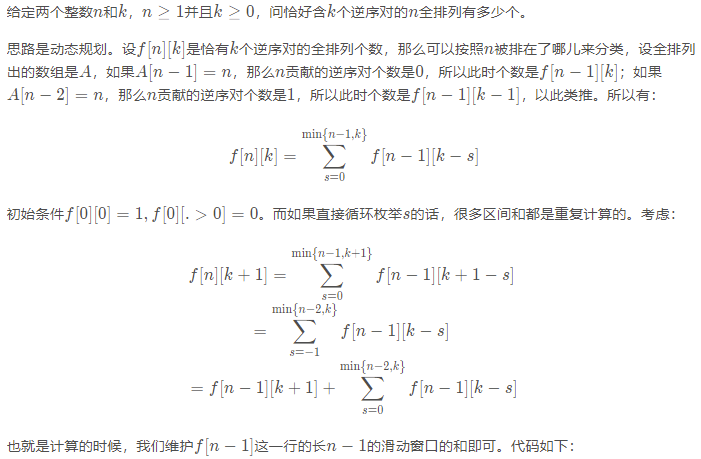
\includegraphics[width=.9\linewidth]{./pic/kinvPair.png}

\begin{minted}[fontsize=\scriptsize,linenos=false]{csharp}
public int kInversePairs(int n, int k) {
    int mod = (int)1e9 + 7;
    int [][] dp = new int [n+1][k+1];
    dp[0][0] = 1;
    for (int i = 1; i <= n; i++) {
        long sum = 0;
        for (int j = 0; j <= k; j++) {
            sum += dp[i-1][j];
            if (j >= i)
                sum -= dp[i-1][j-i];
            dp[i][j] = (int)(sum % mod);
        }
    }
    return (int)dp[n][k];
}
\end{minted}
\end{enumerate}
\subsection{1787. Make the XOR of All Segments Equal to Zero - Hard}
\label{sec-1-4-62}
You are given an array nums​​​ and an integer k​​​​​. The XOR of a segment [left, right] where left <= right is the XOR of all the elements with indices between left and right, inclusive: nums[left] XOR nums[left+1] XOR \ldots{} XOR nums[right].

Return the minimum number of elements to change in the array such that the XOR of all segments of size k​​​​​​ is equal to zero.
\begin{enumerate}
\item 解题思路与分析
\label{sec-1-4-62-0-1}

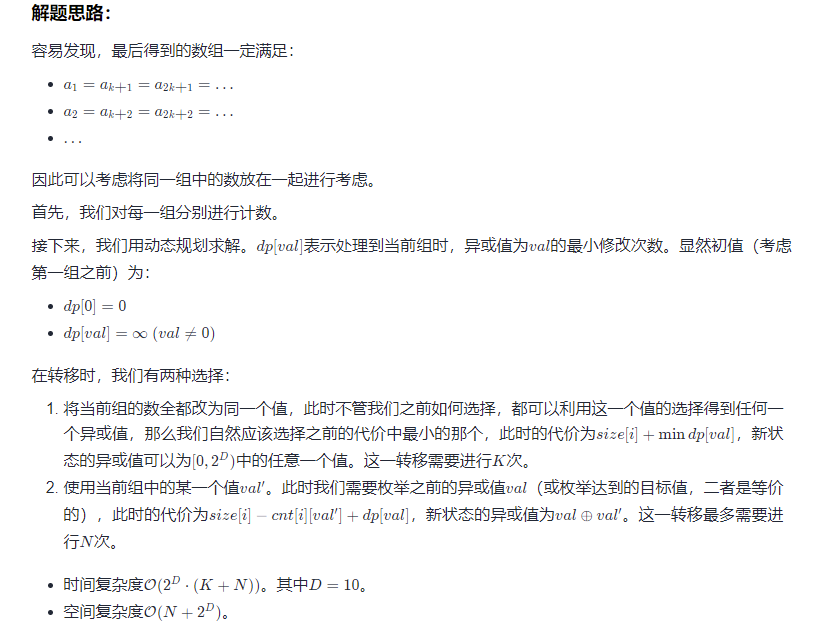
\includegraphics[width=.9\linewidth]{./pic/xortimes.png}

\begin{itemize}
\item 根据题目特点,最后所有长度为 k 的区间异或结果等于零,可推出得到的数组满足:
\end{itemize}
\begin{minted}[fontsize=\scriptsize,linenos=false]{csharp}
a1 = ak+1 = a2k+1 = …
a2 = ak+2 = a2k+2 = …
\end{minted}
因此可将数组中的元素按上述规律,每间隔 k 个的数字为一组进行分组。

在此基础上,设计一个动态规划数组 dp[j],表示到当前第 i 组为止,所有元素异或到对应数字 j 时的更改次数。则对第 i 组 dp[j] 的状态转移方程可能为:

j 可由某一数值和当前组中的某个数 num 异或得到,newDp[j] = dp[j \& num] + size[i] - 组中 num 的数量

j 可通过和任意数字异或得到,newDp[j] = 前一 dp 中最小的改变次数 + size[i]

完成 k 个组的动态规划后,dp\footnotemark[1]{}就是所求的解。

\begin{minted}[fontsize=\scriptsize,linenos=false]{csharp}
public int minChanges(int [] a, int k) {
    int n = a.length;
    Map<Integer, Integer> [] group = new HashMap[k]; // 存储 k 个组、各组中各个数字数量
    int [] cnt = new int [k]; // k元素片段里,每个下标对应的所有元素总个数 // 各组大小,它们会有可能不同吗?
    for (int i = 0; i < k; i++) {
        group[i] = new HashMap<>();
        for (int j = i; j < n; j += k) { // 将数组中的每个元素分布到其在k元素片段中下标位置所在的组里去,并统计重复出现次数
            group[i].put(a[j], group[i].getOrDefault(a[j], 0) + 1);
            cnt[i]++;
        }
    }
    int r = 1 << 10; // 题中nums[i] < 2^10, 为的是遍历所有可能更改值,以取最小
    int [] dp = new int [r], curDp = new int [r]; // 当前组异或到对应数字时的更改次数
    Arrays.fill(dp, Integer.MAX_VALUE);
    dp[0] = 0;
    for (int i = 0; i < k; i++) { // 遍历k个元素的片段——中的每个元素,逐元素优化出全局最优解
        int minVal = Arrays.stream(dp).min().getAsInt(); // 累积到上一个元素的全局最优解
        Arrays.fill(curDp, minVal + cnt[i]); // 变为当前组中不存在数字的改变次数:之前的最小改变次数+当前组元素个数
        for (int j = 0; j < r; j++) {
            if (dp[j] == Integer.MAX_VALUE) continue;
            for (Map.Entry<Integer, Integer> en : group[i].entrySet()) {
                int num = en.getKey(), v = en.getValue(), xorNum = num ^ j;
                curDp[xorNum] = Math.min(curDp[xorNum], dp[j] + cnt[i] - v);
            }
        }
        dp = Arrays.copyOf(curDp, r); // 将遍历到当前组、累积较优解的curDp复制入全局最优解dp数组中
    }
    return dp[0];
}
\end{minted}
\end{enumerate}

\subsection{1735. Count Ways to Make Array With Product - Hard 乘积为K的质因子数排列组合的总个数: 分解质因子}
\label{sec-1-4-63}
You are given a 2D integer array, queries. For each queries[i], where queries[i] = [ni, ki], find the number of different ways you can place positive integers into an array of size ni such that the product of the integers is ki. As the number of ways may be too large, the answer to the ith query is the number of ways modulo 109 + 7.

Return an integer array answer where answer.length == queries.length, and answer[i] is the answer to the ith query.

\begin{enumerate}
\item 解题思路与分析
\label{sec-1-4-63-1}

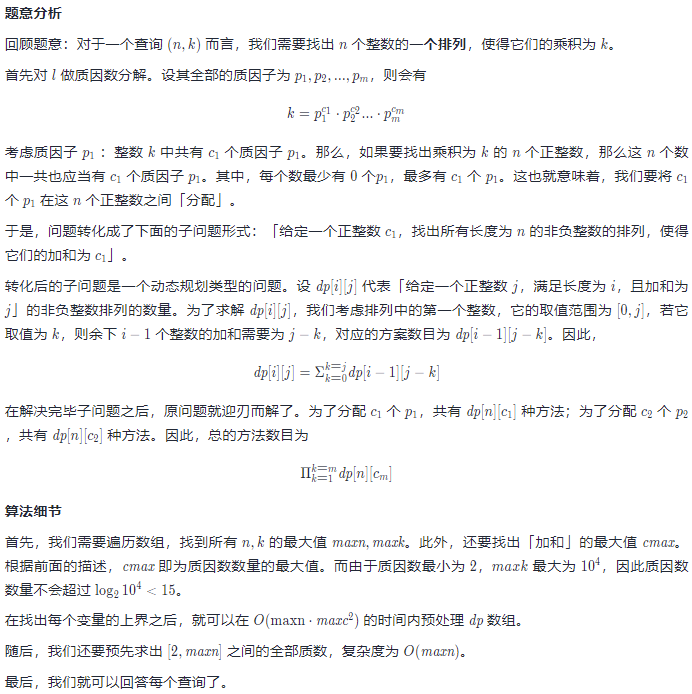
\includegraphics[width=.9\linewidth]{./pic/1735.png}

\begin{minted}[fontsize=\scriptsize,linenos=false]{csharp}
// 在找出每个变量的上界之后,就可以在O(maxn}{maxc}^2)的时间内预处理dp 数组。
//     随后,我们还要预先求出 [2, maxn] 之间的全部质数,复杂度为 O(maxn)。
public int[] waysToFillArray(int[][] q) {
    int n = q.length;
    int mod = (int)1e9 + 7;
    int maxC = 15;          // 找出「加和」的最大值cmax。根据前面的描述,cmax 即为质因数数量的最大值。
    int maxN = 0, maxK = 0; // 而由于质因数最小为 22,maxkmaxk 最大为 10^4因此质因数数量不会超过log_2 10^4 < 15
    for (int i = 0; i < n; i++) { // 需要遍历数组,找到所有 n, kn,k 的最大值maxn,maxk
        maxN = Math.max(maxN, q[i][0]);
        maxK = Math.max(maxK, q[i][1]);
    }
    long [][] dp = new long [maxN + 1][maxC + 1]; // dp[i][j] 代表给定一个正整数 jj,满足长度为 ii,且加和为 jj的非负整数排列的数量。
    for (int i = 1; i <= maxC; i++) 
        dp[1][i] = 1;
    for (int i = 1; i <= maxN; i++) 
        dp[i][0] = 1;
    for (int i = 2; i <= maxN; i++) 
        for (int j = 1; j <= maxC; j++) 
            for (int k = 0; k <= j; k++) { // 为了求解dp[i][j],我们考虑排列中的第一个整数,它的取值范围为 [0,j][0,j],
                dp[i][j] += dp[i-1][j-k];  // 若它取值为 kk,则余下 i-1i−1 个整数的加和需要为 j-kj−k,对应的方案数目为dp[i−1][j−k]
                dp[i][j] %= mod;
            }
    int [] isPrime = new int [maxK + 1]; // 分解乘积的质因子
    Arrays.fill(isPrime, 1);
    List<Integer> primes = new ArrayList<>();
    for (int i = 2; i <= maxK; i++) {
        if (isPrime[i] == 1) 
            primes.add(i);
        for (int j = i*2; j <= i*i && j <= maxK; j += i) // 最大乘积为maxK的数组,分解出小的质因子了,那么凡是小质因子的乘积倍数的数都不是质数
            isPrime[j] = 0;
    }
    int [] ans = new int [n];
    for (int i = 0; i < n; i++) {
        int m = q[i][0], k = q[i][1];
        List<Integer> cs = new ArrayList<>(); // 乘积k的质因子表
        for (int p : primes) {
            if (p > k) break;
            int cnt = 0, left = k;
            while (left % p == 0) {
                left /= p;
                cnt++;
            }
            if (cnt > 0) cs.add(cnt); // 乘积k中各质因子的个数(指数)
        }
        long res = 1;
        for (int c : cs) {
            res *= dp[m][c]; // 数组长度为n,数组和为质因子c的指数个数的所有可能的分布数合数,各质因子之间个数之间相乘
            res %= mod;
        }
        ans[i] = (int)res;
    }
    return ans;
}
\end{minted}
\begin{itemize}
\item 下面这种方法理解得还不是很透
\end{itemize}
\begin{minted}[fontsize=\scriptsize,linenos=false]{csharp}
public int[] waysToFillArray(int[][] queries) {
    int[] result = new int[queries.length];
    int resultIdx = 0;
    Combination combination = new Combination(10030, 20);
    for (int[] q : queries) {
        int n = q[0]; // 长度为n
        int k = q[1]; // 乘积为k
        long product = 1L;
        for (int power : getPrimeFactors(k).values()) {
            // power个球,分到n个位置,每个位置可以为空
            // 等价于:(power+n)个球,分到n个位置,每个位置不能为空  
            // Why? 等价后得到一种分法,每组减去1,就是原来的解
            // 插板法可得 C(power + n - 1, n - 1) = C(power + n - 1, power)
            product = (product * combination.get(n + power - 1, power)) % mod;
        }
        result[resultIdx++] = (int)(product);
    }
    return result;
}
long mod = (int)1e9 + 7;
public HashMap<Integer, Integer> getPrimeFactors(int n) {
    HashMap<Integer, Integer> map = new HashMap();
    for(int i = 2; i <= n; i++) {
        if (n % i == 0) {
            int cnt = 0;
            while (n % i == 0) {
                cnt++;
                n = n / i;
            }
            map.put(i, cnt);
        }
    }
    return map;
}
class Combination {
    long[][] c;
    Combination (int n, int m) {
        c = new long[n + 1][m + 1];
        c[0][0] = 1;
        for(int i = 1; i <= n; i++){
            c[i][0] = 1;
            for(int j = 1; j <= m; j++) 
                c[i][j] = (c[i-1][j-1] + c[i-1][j]) % mod;
        }
    }
    public long get(int n, int m) {
        return c[n][m];
    }
}
\end{minted}
\end{enumerate}

\subsection{1359. Count All Valid Pickup and Delivery Options - Hard}
\label{sec-1-4-64}
Given n orders, each order consist in pickup and delivery services. 

Count all valid pickup/delivery possible sequences such that delivery(i) is always after of pickup(i). 

Since the answer may be too large, return it modulo 10\^{}9 + 7.
\begin{enumerate}
\item 解题思路与分析
\label{sec-1-4-64-0-1}

就是总共有2N个位置,每次放一两个,还剩下多少个位置可以合理占用

\begin{minted}[fontsize=\scriptsize,linenos=false]{csharp}
public int countOrders(int n) {
    int mod = (int)1e9 + 7;
    int spots = n * 2;
    long ans = 1;
    for (int i = n; i >= 2; i--) {
        ans = (ans * spots * (spots - 1) / 2l) % mod;
        spots -= 2;
    }
    return (int)ans;
}
\end{minted}
\end{enumerate}

\subsection{1187. Make Array Strictly Increasing - Hard 需要重写}
\label{sec-1-4-65}
Given two integer arrays arr1 and arr2, return the minimum number of operations (possibly zero) needed to make arr1 strictly increasing.

In one operation, you can choose two indices 0 <= i < arr1.length and 0 <= j < arr2.length and do the assignment arr1[i] = arr2[j].

If there is no way to make arr1 strictly increasing, return -1.
\begin{enumerate}
\item 解题思路与分析
\label{sec-1-4-65-1}
\begin{minted}[fontsize=\scriptsize,linenos=false]{csharp}
public int makeArrayIncreasing(int[] a, int[] b) {
    b = Arrays.stream(b).distinct().toArray();
    Arrays.sort(b);
    int m = a.length, n = b.length;
    int minCnt = 0, minVal = 0;
    Queue<int []> q = new LinkedList<>();
    q.offer(new int [] {-1, 0}); // 初始化,假想第0位的前一位是-1
    for (int i = 0; i < m; i++) {
        minCnt = Integer.MAX_VALUE;
        for (int size = q.size()-1; size >= 0; size--) {
            int [] cur = q.poll(); // 取前一位的一个选择
            if (a[i] > cur[0]) minCnt = Math.min(minCnt, cur[1]); // 先不急将当前选择加入queue中,找到最小的再说
            minVal = binarySearchMin(b, cur[0]); // 查找一个比前一个数大的最小数
            if (minVal != -1) q.offer(new int [] {minVal, cur[1] + 1}); // 将这个最小数加入到queue中,操作次数在前一位的基础上加一
         }
        if (minCnt != Integer.MAX_VALUE) // 如果当前位可以保持不变,将最小次数加入到queue中
            q.offer(new int [] {a[i], minCnt}); 
    }
    if (q.size() == 0) return -1; // 如果最后一位没有合法的选择方案,返回-1
    int ans = Integer.MAX_VALUE;
    while (!q.isEmpty()) ans = Math.min(ans, q.poll()[1]);
    return ans;
}
private int binarySearchMin(int [] arr, int v) {
    int l = 0, r = arr.length-1, m = 0;
    while (l < r) { // l,r: [0, 1]
        m = l + (r-l) / 2;
        if (arr[m] <= v) l = m+1;
        else r = m;
    }
    return arr[l] > v ? arr[l] : -1; // 所以这里要再判断一下
}
\end{minted}
\item 解题思路与分析
\label{sec-1-4-65-2}

这里若是要替换后面的数字为较大的数字,那么就需要在 arr2 中找到比当前数字大的数字,为了让整个数组更容易的递增,那么这个较大数应该尽量越小越好,所以就是要找到第一个比当前数字大的数。为了更容易的在 arr2 中查找,而不是每次都遍历整个数组,需要给 arr2 排个序,然后用二分搜索来查找更高效一些,这里也可以将 arr2 放到一个 TreeSet 中,利用其自动排序的特点,之后再进行二分搜索就行了。这道题的正确解法是用动态规划 Dynamic Programming,这里的 dp 表达式比较难想,一般来说,dp 值都是定义为题目中要求的值,而这道题是个例外,这里的 dp[i][j] 表示对于数组中的前j个数字组成的子数组中,需要替换i次可以使得其变为严格递增,且第j个数字的最小值为 dp[i][j]。这里的 dp 值不是定义为替换次数,而是第j个数字的最小值(可能是替换后的值),因为要保证数组严格递增,最后一个数字的大小很重要,这是个关键信息,而这个数字的大小跟数组坐标之间没有啥必然联系,所以这个信息不太好放到 dp 数组的坐标中,而所求的替换次数跟数组长度是相关的,因为其不可能超过数组的总长度,最差的情况也就是将整个 arr1 数组都替换了(当然还需要考虑 arr2 的长度)。

接下来就来考虑状态转移方程怎么写,由于这里的j表示前j个数字,那么第j个数字实际上是 arr1[j-1],若第j个数字大于 dp[i][j-1],这里表示对于前 j-1 个数字,替换i次可以使得其严格递增,且第 j-1 个数字为 dp[i][j-1],这样的话就不需要额外的替换操作,还是严格递增增的,则 dp[i][j] 可以赋值为 arr1[j-1]。若此时i大于0,说明之前已经进行过替换操作,则上一个操作状态是 dp[i-1][j-1],当前操作是从 arr2 中选一个数字替换 arr1 的第j个数字,这里就要在 arr2 中选择第一个大于 dp[i-1][j-1] 的数字,若存在的话,就用这个数字来更新 dp[i][j] 的值。若某个时刻j等于n了,说明已经到 arr1 的末尾了,若此时 dp[i][j] 不等于 INT\_MAX(初始值),说明是可以将整个 arr1 替换成严格递增的数组的,替换次数就是i,直接返回即可。最终循环退出了,返回 -1,参见代码如下:
\begin{minted}[fontsize=\scriptsize,linenos=false]{cpp}
int makeArrayIncreasing(vector<int>& arr1, vector<int>& arr2) {
    int n = arr1.size();
    if (n == 1) return 0;
    set<int> st(arr2.begin(), arr2.end());
    vector<vector<int>> dp(n + 1, vector<int>(n + 1, INT_MAX));
    dp[0][0] = INT_MIN;
    for (int j = 1; j <= n; ++j) {
        for (int i = 0; i <= j; ++i) {
            if (arr1[j - 1] > dp[i][j - 1]) {
                dp[i][j] = arr1[j - 1];
            }
            if (i > 0) {
                auto it = st.upper_bound(dp[i - 1][j - 1]);
                if (it != st.end()) dp[i][j] = min(dp[i][j], *it);
            }  
            if (j == n && dp[i][j] != INT_MAX) return i;
        }
    }
    return -1;
}
\end{minted}
\end{enumerate}

\section{多维数个数、数种类数 多一维k介入的 dp[i][j][k]}
\label{sec-1-5}
\subsection{1473. Paint House III - Hard}
\label{sec-1-5-1}
There is a row of m houses in a small city, each house must be painted with one of the n colors (labeled from 1 to n), some houses that have been painted last summer should not be painted again.

A neighborhood is a maximal group of continuous houses that are painted with the same color.

For example: houses = [1,2,2,3,3,2,1,1] contains 5 neighborhoods [\{1\}, \{2,2\}, \{3,3\}, \{2\}, \{1,1\}].
Given an array houses, an m x n matrix cost and an integer target where:

houses[i]: is the color of the house i, and 0 if the house is not painted yet.
cost[i][j]: is the cost of paint the house i with the color j + 1.
Return the minimum cost of painting all the remaining houses in such a way that there are exactly target neighborhoods. If it is not possible, return -1.
\begin{enumerate}
\item 解题思路与分析
\label{sec-1-5-1-1}
\begin{minted}[fontsize=\scriptsize,linenos=false]{csharp}
public int minCost(int[] houses, int[][] cost, int m, int n, int target) { // bug
    this.m = m; // 就是最开始: 上一个房子的着色,自顶向下传递的着色 与 自底向上传递的答案之间的交错,最开始理解起来有些理不清楚
    this.n = n;
    dp = new Integer [m][n+1][target+1];
    return dfs(0, 0, target, houses, cost); // 这里始终没能想清楚:初始化的着色0为什么分为不同的街区
}
Integer [][][] dp;
int m, n;
private int dfs(int i, int j, int k, int [] h, int [][] c) { // i: idx, j: color, k: target
    if (k < 0) return -1; 
    if (i == m) return k == 0 ? 0 : -1;
    if (dp[i][j][k] != null) return dp[i][j][k];
    int ans = Integer.MAX_VALUE, v = 0;
    if (h[i] > 0) 
        return dp[i][j][k] = dfs(i+1, h[i], h[i] == j ? k : k-1, h, c); // 如果与上一间房屋颜色不同,开启新街区,target减一 !!!
    for (int x = 0; x < n; x++) {
        v = dfs(i+1, x+1, (x+1 == j ? k : k-1), h, c);
        if (v != -1)
            ans = Math.min(ans, v + c[i][x]);
    }
    return  dp[i][j][k] = ans == Integer.MAX_VALUE ? -1 : ans;
}
\end{minted}
\item 解题思路与分析: DP
\label{sec-1-5-1-2}
\begin{minted}[fontsize=\scriptsize,linenos=false]{csharp}
static final int INFTY = Integer.MAX_VALUE / 2; // 选择 Integer.MAX_VALUE / 2 的原因是防止整数相加溢出
public int minCost(int[] houses, int[][] cost, int m, int n, int target) { // todo: dp 优化解 官方
    // 将颜色调整为从 0 开始编号,没有被涂色标记为 -1
    for (int i = 0; i < m; ++i) --houses[i];
    // dp 所有元素初始化为极大值
    int[][][] dp = new int[m][n][target];
    for (int i = 0; i < m; ++i) 
        for (int j = 0; j < n; ++j) 
            Arrays.fill(dp[i][j], INFTY);
    for (int i = 0; i < m; ++i) 
        for (int j = 0; j < n; ++j) {
            if (houses[i] != -1 && houses[i] != j) continue;
            for (int k = 0; k < target; ++k) {
                for (int x = 0; x < n; x++) {
                    if (j == x) {
                        if (i == 0) {
                            if (k == 0) dp[i][j][k] = 0;
                        } else
                            dp[i][j][k] = Math.min(dp[i][j][k], dp[i-1][j][k]);
                    } else if (i > 0 && k > 0)
                        dp[i][j][k] = Math.min(dp[i][j][k], dp[i-1][x][k-1]);
                }
                if (dp[i][j][k] != INFTY && houses[i] == -1)
                    dp[i][j][k] += cost[i][j];
            }
        }
    int ans = INFTY;
    for (int j = 0; j < n; ++j) 
        ans = Math.min(ans, dp[m - 1][j][target - 1]);
    return ans == INFTY ? -1 : ans;
}
\end{minted}
\end{enumerate}

\subsection{1223. Dice Roll Simulation - Hard}
\label{sec-1-5-2}
A die simulator generates a random number from 1 to 6 for each roll. You introduced a constraint to the generator such that it cannot roll the number i more than rollMax[i] (1-indexed) consecutive times.

Given an array of integers rollMax and an integer n, return the number of distinct sequences that can be obtained with exact n rolls. Since the answer may be too large, return it modulo 109 + 7.

Two sequences are considered different if at least one element differs from each other.
\begin{enumerate}
\item 解题思路与分析: dfs记忆化搜索
\label{sec-1-5-2-1}
\begin{minted}[fontsize=\scriptsize,linenos=false]{csharp}
public int dieSimulator(int n, int [] r) { // dfs记忆化搜索:数据传递时,自顶向下传递的同一个值出现的次数, 与自底向上返回的方案数的交互,要熟悉起来,
    dp = new Integer [7][16][n+1];         // 最开始的dp定义想的是对的, 与房子涂成几个街区类似
    return (int)dfs(0, 0, n, r);
}
static final int mod = (int)1e9 + 7;
Integer [][][] dp;
private long dfs(int i, int j, int k, int [] cnt) { // i: val, j: continuous cnt, k: cnt out of n times
    if (k == 0) return 1;
    if (dp[i][j][k] != null) return dp[i][j][k];
    long ans = 0;
    for (int x = 1; x <= 6; x++) {
        if (x == i && cnt[x-1] > j)
            ans = (ans + dfs(x, j+1, k-1, cnt)) % mod;
        else if (x != i)
            ans = (ans + dfs(x, 1, k-1, cnt)) % mod;
    }
    return dp[i][j][k] = (int)ans;
}
\end{minted}
\item 解题思路与分析: dp
\label{sec-1-5-2-2}
\begin{minted}[fontsize=\scriptsize,linenos=false]{csharp}
// (动态规划) O(nm)
// f(i,j,k) 表示前 i 次投,最后一次结果为 j 且最后的数字连续了 k 次的方案数。
// 初始时,f(0,j,1) = 1,其余均为 0。
// 转移时,对于每一个 i和 j,枚举上一次最后的结果 t,如果 j==t,则转移f(i,j,k)=f(i,j,k)+f(i−1,j,k−1);否则f(i,j,1)=f(i,j,1)+f(i−1,t,k)。
//     最终答案为f(n−1,j,k) 的总和。
static final long mod = (int)1e9 + 7;
public int dieSimulator(int n, int [] r) { // 因为第三个限制条件的出现,而增加到三维dp[i][j][k]题型 ,总结一下
    long [][][] dp = new long [n][6][16]; 
    for (int i = 0; i < 6; i++) dp[0][i][1] = 1; // 第一次投掷,各个数出现一次的次数均为1
    for (int i = 1; i < n; i++) 
        for (int j = 0; j < 6; j++) 
            for (int x = 0; x < 6; x++)  // x t: 把它当作上一次的最后结果 
                if (j == x) 
                    for (int k = 2; k <= r[j]; k++) 
                        dp[i][j][k] = (dp[i][j][k] + dp[i-1][j][k-1]) % mod;
                else for (int k = 1; k <= r[x]; k++) // 因为是新的数字出现,没有任何限制,所以把前面的结果全累积起来
                        dp[i][j][1] = (dp[i][j][1] +  dp[i-1][x][k]) % mod;
    long ans = 0;
    for (int j = 0; j < 6; j++)
        for (int k = 1; k <= r[j]; k++) 
            ans = (ans + dp[n-1][j][k]) % mod;
    return (int) ans;
}
\end{minted}
\end{enumerate}

\subsection{920. Number of Music Playlists - Hard}
\label{sec-1-5-3}
Your music player contains n different songs. You want to listen to goal songs (not necessarily different) during your trip. To avoid boredom, you will create a playlist so that:

Every song is played at least once.
A song can only be played again only if k other songs have been played.
Given n, goal, and k, return the number of possible playlists that you can create. Since the answer can be very large, return it modulo 109 + 7.
\begin{enumerate}
\item 解题思路与分析
\label{sec-1-5-3-1}

当加入的是一首新歌,则表示之前的 L-1 首歌中有 j-1 首不同的歌曲,其所有的组合情况都可以加上这首新歌,那么当前其实有 N-(j-1) 首新歌可以选。

当加入的是一首重复的歌,则表示之前的 L-1 首歌中已经有了 j 首不同的歌,那么若没有K的限制,则当前有 j 首重复的歌可以选。但是现在有了K的限制,意思是两首重复歌中间必须要有K首其他的歌,则当前只有 j-K 首可以选。而当 j<k 时,其实这种情况是为0的。<="" li="" >

综上所述可以得到状态转移方程:

\begin{minted}[fontsize=\scriptsize,linenos=false]{csharp}
            dp[i-1][j-1]*(N-(j-1)) + dp[i-1][j]*(j-k)    (j > K)	
           /	
dp[i][j] = 	
           \	
            dp[i-1][j-1] x (N-(j-1))   (j <= K)
\end{minted}
\begin{minted}[fontsize=\scriptsize,linenos=false]{csharp}
public int numMusicPlaylists(int n, int goal, int k) {
    long mod = (int)1e9 + 7;
    long [][] dp = new long [goal+1][n+1]; // dp[i][j]: 播完i首用了j首不同的曲子,分第i首播不播第j首两种情况 (i >= j for sure)
    for (int i = 1; i <= goal; i++) 
        for (int j = 1; j <= n; j++) {
            if (i < j) dp[i][j] = 0; // 这行不能省略   
            else if (i == 1 && j == 1) dp[i][j] = n; // 用1首歌放完1次,共有n种不同的选择
            else if (i > 1 && j == 1) {
                if (k == 0) dp[i][j] = n; // 相当于没有任何外加限制条件
                // else dp[i][1] = 0;     // 这行可略
            } else // 分两种情况: 第i首不播第j首歌(那么可以从前面j-k首里面选择一首),和第i首播第j首歌(第j首就可以从不曾播放过的n-(j-1)首里面选择一首播放)
                dp[i][j] = (dp[i-1][j] * Math.max(j-k, 0) + (j == 0 ? 0 : dp[i-1][j-1] * (n - (j-1)))) % mod;
        }
    return (int)dp[goal][n];
}
\end{minted}
\begin{itemize}
\item 简化一下代码
\end{itemize}
\begin{minted}[fontsize=\scriptsize,linenos=false]{csharp}
static final int mod = (int)1e9 + 7;
public int numMusicPlaylists(int n, int goal, int k) {
    long [][] dp = new long [goal+1][n+1]; // dp[i][j]: 播完i首用了j首不同的曲子,分第i首播不播第j首两种情况 (i >= j for sure)
    dp[0][0] = 1;
    for (int i = 1; i <= goal; i++) 
        for (int j = 1; j <= n; j++) {
            dp[i][j] = (dp[i-1][j-1] * (n - (j-1))) % mod; // 第j首放新歌
            if (j > k)                                     // 第j首放(j-k)之前的某首歌
                dp[i][j] = (dp[i][j] + dp[i-1][j] * (j-k)) % mod;
        }
    return (int)dp[goal][n];
}
\end{minted}
\end{enumerate}

\subsection{1866. Number of Ways to Rearrange Sticks With K Sticks Visible - Hard}
\label{sec-1-5-4}
There are n uniquely-sized sticks whose lengths are integers from 1 to n. You want to arrange the sticks such that exactly k sticks are visible from the left. A stick is visible from the left if there are no longer sticks to the left of it.

For example, if the sticks are arranged [1,3,2,5,4], then the sticks with lengths 1, 3, and 5 are visible from the left.
Given n and k, return the number of such arrangements. Since the answer may be large, return it modulo 109 + 7.
\begin{minted}[fontsize=\scriptsize,linenos=false]{csharp}
// dp[i][j] 表示前面i根木棍可以看到j根
// 设 dp[i][j] 表示从高度为 1, 2, ..., i 的木棍中,高度逐渐递减地插入新的木棍,从左侧看恰好看到 k 根木棍的方案数。
// 后面说看到ith根,不是指从小到大的第ith根棍子,而是指ith这个位置上的棍子
// 如果可以看到ith根的话,那么数量为dp[i-1][j-1]
// 如果看不到ith的话,那么取前面(i-1)里面任意一个出来放在ith的最后,接下来就是从前面i-1个棍子里面看到j根,所以结果是 (i-1)* dp[i-1][j]
public int rearrangeSticks(int n, int k) {
    int mod = (int)1e9 + 7;
    long [][] dp = new long [n+1][k+1];
    dp[0][0] = 1;
    for (int i = 1; i <= n; i++) 
        for (int j = 1; j <= k; j++) 
            dp[i][j] = (dp[i-1][j-1] + (i - 1) * dp[i-1][j]) % mod;
    return (int)dp[n][k];
}
\end{minted}
\begin{itemize}
\item dfs + memo
\end{itemize}
\begin{minted}[fontsize=\scriptsize,linenos=false]{csharp}
public int rearrangeSticks(int n, int k) {
    dp = new long [n+1][k+1];
    return (int)dfs(n, k);
}
int mod = (int)1e9 + 7;
long [][] dp;
private long dfs(int n, int k) {
    if (n < k || k == 0) return 0;
    if (n == k) return 1;
    if (dp[n][k] != 0) return dp[n][k];
    // instead of iterating for every stick
    // we are just multiplying number of ways with (n - 1)
    return dp[n][k] = (dfs(n-1, k-1) + (n - 1) * dfs(n-1, k)) % mod;
}
\end{minted}

\subsection{1916. Count Ways to Build Rooms in an Ant Colony - Hard}
\label{sec-1-5-5}
You are an ant tasked with adding n new rooms numbered 0 to n-1 to your colony. You are given the expansion plan as a 0-indexed integer array of length n, prevRoom, where prevRoom[i] indicates that you must build room prevRoom[i] before building room i, and these two rooms must be connected directly. Room 0 is already built, so prevRoom\footnotemark[1]{} = -1. The expansion plan is given such that once all the rooms are built, every room will be reachable from room 0.

You can only build one room at a time, and you can travel freely between rooms you have already built only if they are connected. You can choose to build any room as long as its previous room is already built.

Return the number of different orders you can build all the rooms in. Since the answer may be large, return it modulo 109 + 7.

对每个节点,可根据所有以其子节点为根的树的节点及排列数量,计算出以当前节点为根的树的节点及排列数量。

本题求解过程涉及较多前置知识点,包括排列组合、乘法逆元、快速乘方等

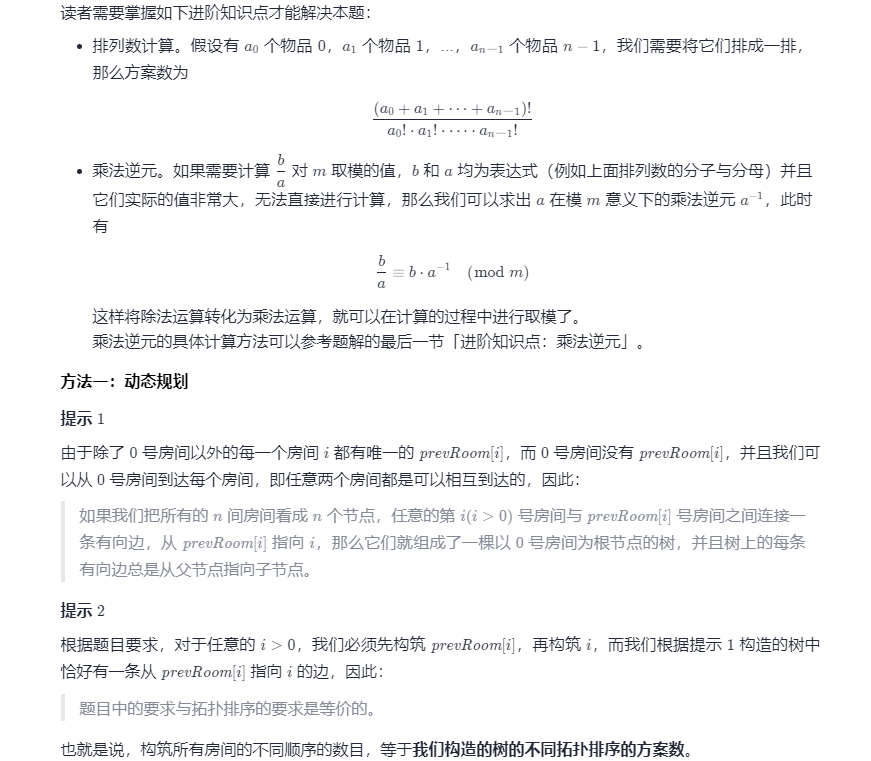
\includegraphics[width=.9\linewidth]{./pic/ant1.png}

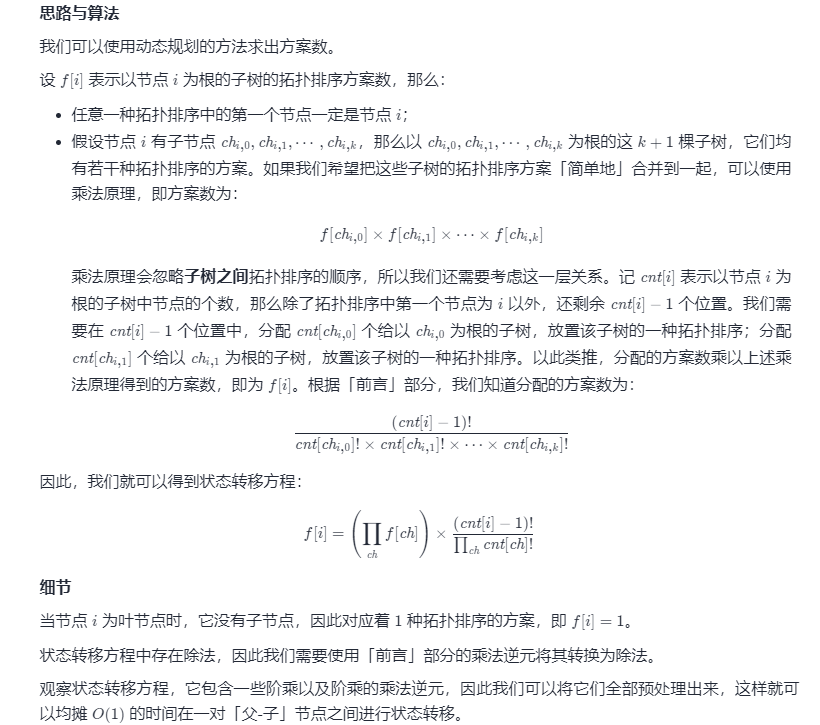
\includegraphics[width=.9\linewidth]{./pic/ant2.png}

\begin{minted}[fontsize=\scriptsize,linenos=false]{csharp}
static final int mod = (int)1e9 + 7;
public int waysToBuildRooms(int[] prevRoom) {
    int n = prevRoom.length;
    // 求阶乘数列及对应逆元
    this.fac = new int [n]; // fac[i]=i!
    this.inv = new int [n]; // inv[i]=i!^(-1)
    fac[0] = inv[0] = 1;
    for (int i = 1; i < n; i++) {
        fac[i] = (int)((long)fac[i-1] * i % mod); // 算阶层
        inv[i] = quickMultiply(fac[i], mod - 2);  // 乘法逆元:费马小定理 : (fac[i]^(-1))%mod = (fac[i]^(mod-2))%mod 转换成快速幂操作
    }
    for (int i = 0; i < n; i++) // 记录各个节点与子节点之间的边
        m.computeIfAbsent(prevRoom[i], z -> new ArrayList<>()).add(i);
    return dfs(0)[1]; // 动态规划得到总体顺序数量x
}
Map<Integer, List<Integer>> m = new HashMap<>();
int [] fac, inv;  
private int [] dfs(int idx) { // 返回以当前节点为根的子树节点个数 及 内部排列数
    if (!m.containsKey(idx)) return new int [] {1, 1}; // 子节点,节点个数及内部排列数均为1
    int cnt = 1, ans = 1; // 子树的结点个数、内部排列数
    for (Integer next : m.get(idx)) {
        int [] cur = dfs(next); // 递归得到子节点对应树的节点个数和排列数
        cnt += cur[0];
        ans = (int)((long)ans * cur[1] % mod * inv[cur[0]] % mod);
    }
    ans = (int)((long)ans * fac[cnt-1] % mod);
    return new int [] {cnt, ans} ;
}
private int quickMultiply(int x, int y) { // 快速幂: 快速计算x^y的乘方
    long ans = 1, base = x;
    while (y > 0) {
        if ((y & 1) == 1)
            ans = (ans * base) % mod; // 指数是奇数次,就先乘一次底数
        base = base * base % mod; // 指数剩偶数次了,就可以直接底数先平方,指数除以2
        y >>= 1; // 指数除2
    }
    return (int) ans;
}
\end{minted}

\subsection{1504. Count Submatrices With All Ones - Medium}
\label{sec-1-5-6}
Given an m x n binary matrix mat, return the number of submatrices that have all ones.
\begin{enumerate}
\item 解题思路与分析
\label{sec-1-5-6-1}

首先我们对矩阵进行数据初始化。即求出每一行以及每一列上的前缀和。

遍历矩阵每一个点(两层循环),并以该点最为起点(row, col),向右下方向画矩形(两层循环,分别循环矩形的宽width和高height),注意矩形范围不能越界。起始时width和height分别为0,即当前点自身是一个矩形。

当width扩大一格后,实际上是增加了(row, col+width)到(row+height, col+width)这一部分的面积(宽为width,高为height),我们通过前缀和数组求出该区域和是否等于height,如果等于,返回结果加一即可。

width扩大一格的操作同理。
\begin{minted}[fontsize=\scriptsize,linenos=false]{csharp}
public int numSubmat(int[][] mat) {
    int m = mat.length, n = mat[0].length;
    int [][] row = new int [m][n]; // 每一行的前缀和
    int [][] col = new int [m][n]; // 每一列的前缀和
    for (int i = 0; i < m; i++)
        for (int j = 0; j < n; j++) 
            row[i][j] = (j == 0 ? 0 : row[i][j-1]) + mat[i][j];
    for (int j = 0; j < n; j++) 
        for (int i = 0; i < m; i++) 
            col[i][j] = (i == 0 ? 0 : col[i-1][j]) + mat[i][j];
    int ans = 0;
    for (int i = 0; i < m; i++) 
        for (int j = 0; j < n; j++) 
            for (int r = 0; i+r < m; r++)       // 以当前点为顶点,向下扩大一格, r = 0 起点是0,当前格自身也是答案
                for (int c = 0; j+c < n; c++) { // 以当前点为顶点,向右扩大一格
                    int x = i + r, y = j + c;
                    // 数新扩张区域内每行每列区域内长度累加和都等于长度,即新增区域每格都是1
                    if ((j == 0 && row[x][y] == c+1 || j > 0 && row[x][y] - row[x][j-1] == c+1)
                        && (i == 0 && col[x][y] == r+1 || i > 0 && col[x][y] - col[i-1][y] == r+1))
                        ans++;
                    else break;
                }
    return ans;
}
\end{minted}
\item 解题思路与分析: 单调栈 todo
\label{sec-1-5-6-2}
\begin{minted}[fontsize=\scriptsize,linenos=false]{csharp}
private int res = 0;
private int n;
public int numSubmat(int[][] mat) {
    this.n = mat[0].length;
    // dp[j] : the height (number of consecutive '1's) of column j 
    int[] dp = new int[n];
    for (int i = 0; i < mat.length; i++) {
        // calculating (updating) heights
        for (int j = 0; j < n; j++) 
            dp[j] = mat[i][j] == 1 ? dp[j] + 1 : 0;
        enumerateRowByMinHeight(dp);
    }
    return res;
}
public void enumerateRowByMinHeight(int[] dp) {
    // monotonic stack storing indices : for index p < q in stack, dp[p] < dp[q]
    Deque<Integer> stack = new LinkedList<>();
    stack.offerLast(-1);
    for (int j = 0; j < n; j++) {
        while (stack.peekLast() != -1 && dp[stack.peekLast()] >= dp[j]) {
            int idx = stack.pollLast();
            res += dp[idx] * (idx - stack.peekLast()) * (j - idx);
        }
        stack.offerLast(j);
    }
    while (stack.peekLast() != -1) {
        int idx = stack.pollLast();
        res += dp[idx] * (idx - stack.peekLast()) * (n - idx);
    }
}
\end{minted}
\begin{minted}[fontsize=\scriptsize,linenos=false]{csharp}
// Used two Arrays to store number of consecutive ones on the left, and number of consecutive ones above(up)
//     In one m*n loop we can count the number of order 1xM rectangles where M belongs to [1,m-1]
//     and we can count rectangles of order MxN each time where M>1. in the k index loop.
public int numSubmat(int[][] mat) {
    int m = mat.length, n = mat[0].length;
    int [][] left = new int [m][n]; // 每一行的前缀和
    int [][] abov = new int [m][n]; // 每一列的前缀和
    int ans = 0;
    for (int i = 0; i < m; i++) 
        for (int j = 0; j < n; j++) 
            if (mat[i][j] == 1)  {
                left[i][j] = (j == 0 ? 0 : left[i][j-1]) + 1;
                ans += (j == 0 ? 1 : left[i][j]);
                abov[i][j] = (i == 0 ? 0 : abov[i-1][j]) + 1;
                if (i > 0) {
                    int min = left[i][j];
                    for (int k = 1; k < abov[i][j]; k++) {
                        min = Math.min(min, left[i-k][j]);
                        ans += min;
                    }
                }
            }
    return ans;
}
\end{minted}
\begin{minted}[fontsize=\scriptsize,linenos=false]{csharp}
// In the first pass through the matrix, we store the heights of 1s above a given i,j
// In the second pass, we go through each element that is nonzero, scan leftwards,
//     adding the minimum of the heights encountered until we reach the beginning of the row or hit a zero.
public int numSubmat(int[][] mat) {
    int m = mat.length, n = mat[0].length;
    for (int j = 0; j < n; j++) {
        int colsum = 0;
        for (int i = 0; i < m; i++) {
            if (mat[i][j] == 0) colsum = 0;
            else colsum += mat[i][j];
            mat[i][j] = colsum;
        }
    }
    int tot = 0;
    for (int i = 0; i < m; i++) 
        for (int j = 0; j < mat[i].length; j++) {
            int k = j;
            int min = Integer.MAX_VALUE;
            while (k >= 0 && mat[i][k] != 0) {
                min = Math.min(min, mat[i][k]);
                tot += min;
                k--;
            }
        }
    return tot;
}
\end{minted}
\end{enumerate}
\subsection{1621. Number of Sets of K Non-Overlapping Line Segments - Medium}
\label{sec-1-5-7}
Given n points on a 1-D plane, where the ith point (from 0 to n-1) is at x = i, find the number of ways we can draw exactly k non-overlapping line segments such that each segment covers two or more points. The endpoints of each segment must have integral coordinates. The k line segments do not have to cover all n points, and they are allowed to share endpoints.

Return the number of ways we can draw k non-overlapping line segments. Since this number can be huge, return it modulo 109 + 7.
\begin{enumerate}
\item 解题思路与分析: dfs记忆化搜索, 很慢很慢很慢。。。。。。
\label{sec-1-5-7-1}
\begin{minted}[fontsize=\scriptsize,linenos=false]{csharp}
public int numberOfSets(int n, int k) { 
    if (k == n-1) return 1;
    this.n = n;
    dp = new Long [n][k+1];
    return (int)dfs(0, k);
}
long mod = (int)1e9 + 7;
Long [][] dp; // have to be Long, Integer overflow
int n;
private long dfs(int idx, int k) {
    if (dp[idx][k] != null) return dp[idx][k];
    if (k == 0) return 1;
    long ans = 0;
    for (int i = idx+1; i < n; i++)
        ans += (i - idx) * dfs(i, k-1);
    return dp[idx][k] = ans % mod;
}
\end{minted}
\item 解题思路与分析: dp[i][j][k]
\label{sec-1-5-7-2}

记 f[i][j]f[i][j] 表示使用 0 .. i 的点构造了 jj 条线段的方案数。我们需要区分第 jj 条线段的右端点是否就是 ii,因此可以考虑把 f[i][j] 拆分成两个状态:

\begin{itemize}
\item f[i][j]\footnotemark[1]{} 表示第 jj 条线段的右端点不是 ii,也就是说我们没有办法继续延长第 jj 条线段;
\item f[i][j]\footnotemark[2]{} 表示第 jj 条线段的右端点就是 ii,也就是说我们可以选择是否继续延长第 jj 条线段。
\end{itemize}

如何进行状态转移呢?

首先考虑 f[i][j]\footnotemark[1]{}f[i][j]\footnotemark[1]{},因为第 jj 条线段的右端点不是 ii,因此第 ii 个点没有用上,那么 0 .. i-1 的点构造了 jj 条线段,即

\begin{itemize}
\item f[i][j]\footnotemark[1]{} = f[i-1][j]\footnotemark[1]{} + f[i-1][j]\footnotemark[2]{}
\end{itemize}

再考虑 f[i][j]\footnotemark[2]{}f[i][j]\footnotemark[2]{},因为第 jj 条线段的右端点就是 ii,因此有两种情况:

第 jj 条线段长度为 11,那么 0 .. i-1 的点构造了 j-1j−1 条线段,即

\begin{itemize}
\item f[i][j]\footnotemark[2]{} = f[i-1][j-1]\footnotemark[1]{} + f[i-1][j-1]\footnotemark[2]{}
\end{itemize}

第 jj 条线段长度大于 11,那么删去第 jj 条线段 i-1 .. i 的这一部分,0 .. i-1 的点仍然构造了 jj 条线段,并且点 i-1i−1 是属于第 jj 条线段的,即

\begin{itemize}
\item f[i][j]\footnotemark[2]{} = f[i-1][j]\footnotemark[2]{}
\end{itemize}

加上边界条件 f\footnotemark[1]{}\textsuperscript{,}\,\footnotemark[1]{}\textsuperscript{,}\,\footnotemark[1]{} = 1,最终答案即为 f[n-1][k]\footnotemark[1]{} + f[n-1][k]\footnotemark[2]{}.

\begin{minted}[fontsize=\scriptsize,linenos=false]{csharp}
public int numberOfSets(int n, int k) {
    int mod = (int)1e9 + 7;
    long [][][] dp = new long [n][k+1][2]; // dp[i][j][0/1]: 0, 1, 2 ... i形成j段线段,并且第j段线段是1(否0)以点i结尾
    dp[0][0][0] = 1;
    for (int i = 1; i < n; i++) {
        for (int j = 0; j <= k; j++) {
            dp[i][j][0] = (dp[i-1][j][0] + dp[i-1][j][1]) % mod;
            dp[i][j][1] = dp[i-1][j][1];
            if (j > 0)
                dp[i][j][1] = (dp[i][j][1] + dp[i-1][j-1][0] + dp[i-1][j-1][1]) % mod; 
        }
    }
    return (int)((dp[n-1][k][0] + dp[n-1][k][1]) % mod);
}
\end{minted}
\item 解题思路与分析: dp[i][j]
\label{sec-1-5-7-3}

dp[i][j] means how many number of ways we cut j segments for first i points. The result will be dp[n - 1][k]

It is easy to come up with O(N * N * K) solutions
\begin{minted}[fontsize=\scriptsize,linenos=false]{csharp}
1. Initial value: dp[0][0] = 1. It is only 1 ways to cut first 0 points to 0 segments.
2. For i > 0, dp[i][j] = dp[i - 1][j]. This is assuming that we don't have jth segment ends up with i th points but j segments can be formed by first i - 1 points.
3. Now lets' handle those cases that j th segment which will ends up with ith points. jth segments length varies.
\end{minted}

dp[i][j] = sum(dp\footnotemark[1]{}[j - 1] \ldots{}.. dp[i - 1][j - 1])

\begin{minted}[fontsize=\scriptsize,linenos=false]{csharp}
int mod = 1_000_000_007;                // tle
public int numberOfSets(int n, int k) { // tle
    long[][] dp = new long[n][k + 1];
    dp[0][0] = 1;
    for (int i = 0; i < n; i++) 
        for (int j = 0; j <= Math.min(k, i); j++) {
            if (i > 0) dp[i][j] = dp[i - 1][j];
            if (j > 0) 
                for (int h = i - 1; h >= 0; h--) 
                    dp[i][j] = (dp[i][j] + dp[h][j - 1]) % mod;
        }
    return (int)dp[n - 1][k];
}
\end{minted}

\begin{itemize}
\item However it won't pass LC, because the time complexity is too high. Let's optimize it. We can see the inner for loop. It counts ALL values of dp[0\ldots{}i - 1][j - 1].
\end{itemize}
\begin{minted}[fontsize=\scriptsize,linenos=false]{csharp}
for (int h = i - 1; h >= 0; h--) 
    dp[i][j] = (dp[i][j] + dp[h][j - 1]) % mod;
\end{minted}

\begin{itemize}
\item We can use a new array to store the previous sum of it. In this way, we don't need compute again. In order to use previous sum, we have to reverse the order of for (int j = 0; j <= Math.min(k, i); j++) to for (int j = Math.min(k, i); j >= 0; j--).
\end{itemize}
\begin{minted}[fontsize=\scriptsize,linenos=false]{csharp}
int mod = 1_000_000_007;
public int numberOfSets(int n, int k) {
    long[][] dp = new long[n][k + 1];
    dp[0][0] = 1;
    long[] sums = new long[k + 1];
    for (int i = 0; i < n; i++) 
        for (int j = Math.min(k, i); j >= 0; j--) {
            if (i > 0) dp[i][j] = dp[i - 1][j];
            if (j > 0) dp[i][j] = (sums[j - 1] + dp[i][j]) % mod;
            sums[j] = (sums[j] + dp[i][j]) % mod;
        }
    return (int)dp[n - 1][k];
}
\end{minted}
\end{enumerate}

\section{BitMask掩码相关的}
\label{sec-1-6}

\chapter{dfs 记忆化搜索}
\label{sec-2}
\subsection{1977. Number of Ways to Separate Numbers - Hard}
\label{sec-2-0-1}
You wrote down many positive integers in a string called num. However, you realized that you forgot to add commas to seperate the different numbers. You remember that the list of integers was non-decreasing and that no integer had leading zeros.

Return the number of possible lists of integers that you could have written down to get the string num. Since the answer may be large, return it modulo 109 + 7.
\begin{enumerate}
\item 动态规划: 与最长公共前缀
\label{sec-2-0-1-1}

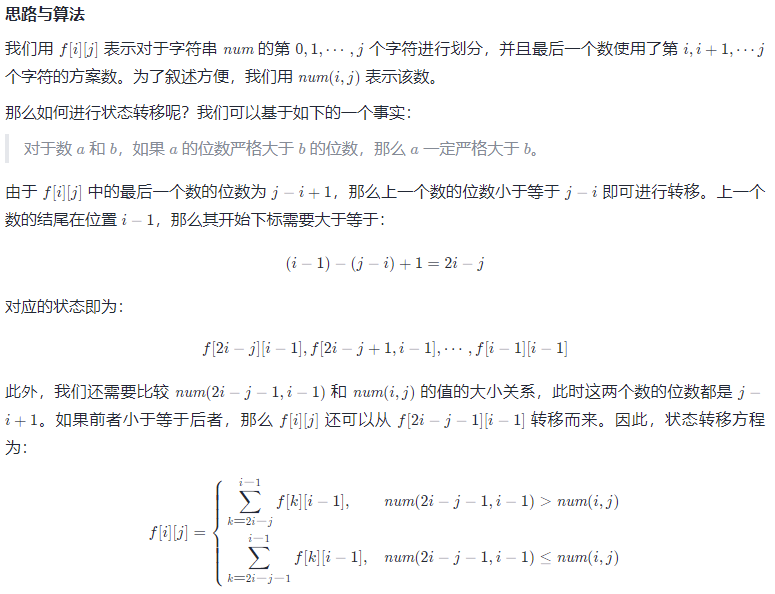
\includegraphics[width=.9\linewidth]{./pic/1977-1.png}

需要注意的是:为了防止状态转移方程显得过于复杂,我们在状态转移方程中:

没有考虑2i−j 和 2i−j−1 是否超出边界。但在实际的代码编写中,需要保证求和式中 kk 的最小值不能小于 00;

没有考虑 num(i,j) 是否包含前导零。如果num[i]=0,那么f[i][j]=0。特别地,如果num\footnotemark[1]{}=0,那么不会有任何满足要求的划分方案,直接返回 00 作为答案,无需进行动态规划。

动态规划的边界条件为 f\footnotemark[1]{}[..] = 1其余的状态的初始值均为 00。最终的答案即为所有 f[..][n - 1]f[..][n−1] 的和,其中 nn 是字符串 num\}num 的长度。

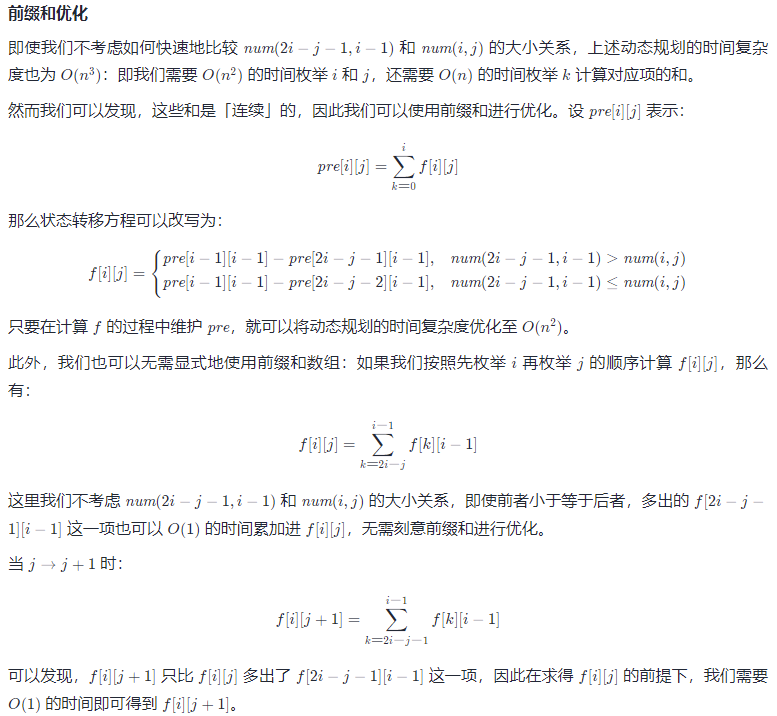
\includegraphics[width=.9\linewidth]{./pic/1977-2.png}

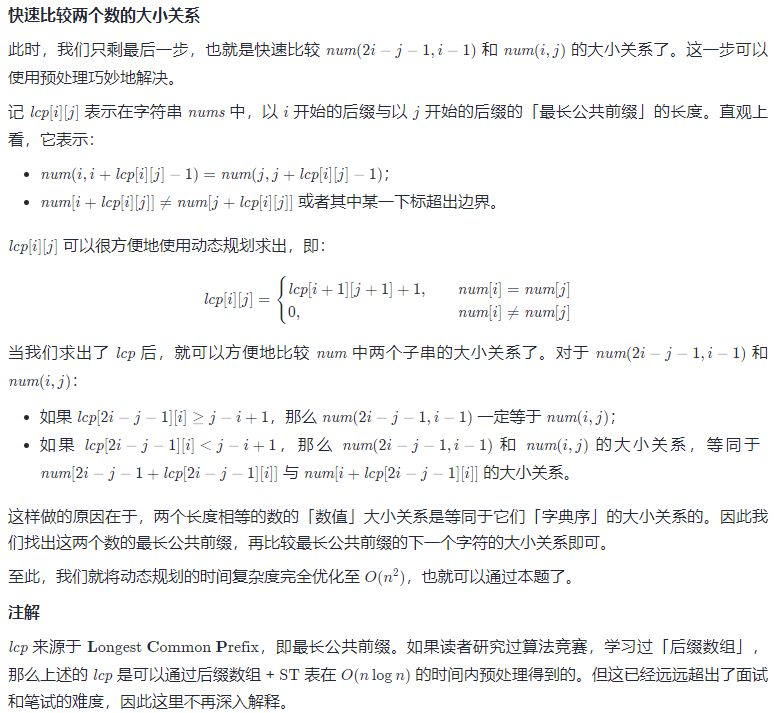
\includegraphics[width=.9\linewidth]{./pic/1977-3.png}

\begin{minted}[fontsize=\scriptsize,linenos=false]{csharp}
static final int mod = (int)1e9 + 7;
public int numberOfCombinations(String t) {
    int n = t.length();
    char [] s = t.toCharArray();
    if (s[0] == '0') return 0;
    int [][] lcp = new int [n][n];   // 求的是: 以s[i]开始的后缀,与以s[j]开始的后缀,两字符串的最长公共前缀长度
    for (int i = n-1; i >= 0; i--) { // 预处理 lcp
        lcp[i][n-1] = s[i] == s[n-1] ? 1 : 0;
        for (int j = i+1; j < n-1; j++) 
            lcp[i][j] = s[i] == s[j] ? lcp[i+1][j+1] + 1 : 0;
    }
    int [][] dp = new int [n][n];
    for (int i = 0; i < n; i++) dp[0][i] = 1; // dp[0][...] = 1
    for (int i = 1; i < n; i++) {
        if (s[i] == '0') continue; // 有前导零,无需转移
        int preSum = 0;
        for (int j = i; j < n; j++) {
            int length = j - i + 1; // s[i,j]
            dp[i][j] = preSum;      // dp[i][j] = d[i][j-1] + (one item) // 这里是j 从 i开始累加的dp[...]前缀和
            if (i - length >= 0) {  // 使用 lcp 比较 s[2i-j-1,i-1] 与 s[i,j] 的大小关系
                if (lcp[i-length][i] >= length || s[i - length + lcp[i-length][i]] < s[i + lcp[i-length][i]])
                    dp[i][j] = (dp[i][j] + dp[i-length][i-1]) % mod;
                preSum = (preSum + dp[i-length][i-1]) % mod; // 更新前缀和,这里是 j 从 i 开始累加的dp[...]前缀和
            }
        }
    }
    int ans = 0;
    for (int i = 0; i < n; i++) // 最终答案即为所有 dp[..][n-1] 的和
        ans = (ans + dp[i][n-1]) % mod;
    return ans;
}
\end{minted}
\begin{itemize}
\item 另一种写法
\end{itemize}
\begin{minted}[fontsize=\scriptsize,linenos=false]{csharp}
private void getLongestCommonPrefixLength() { // Pre compute Longest Common Prefix sequence for each index in the string
    for (int i = n-1; i >= 0; i--)            // 从右向左遍历,计算最长公共前缀序列长度
        for (int j = n-1; j >= 0; j--) 
            if (s[i] == s[j]) {
                if (i >= n-1 || j >= n-1) lcp[i][j] = 1;
                else lcp[i][j] = lcp[i+1][j+1] + 1;
            } else lcp[i][j] = 0;
}
private boolean compare(int i, int j, int len) { // compare substring of same length for value, 
    int commonLength = lcp[i][j];                // 返回以i开始长度为len的序列 是否 比以j开始长度为len的序列(数值)小
    if (commonLength >= len) return true;
    return  s[i + commonLength] <= s[j + commonLength]; // <= ? 为什么不可以等于呢?
}
long mod = (int)1e9 + 7;
int [][] lcp;
char [] s; 
int n;
public int numberOfCombinations(String t) {
    if (t.charAt(0) == '0') return 0;
    n = t.length();
    this.s = t.toCharArray();
    lcp = new int[n][n];
    int [][] f = new int [n][n];
    int [][] pre = new int [n][n];  // 从右向左的累加和
    getLongestCommonPrefixLength(); // 计算从右向左遍历的最长公共前缀(右边,其实是后缀)
    for (int i = 0; i < n; i++) {
        f[0][i] = 1;
        pre[0][i] = 1;
    }
    for (int j = 1; j < n; j++) { // 跟上面超内存的写法是反着走,这次是从左向右遍历,可是两种方法,为什么就有一个会超内存呢?
        for (int i = 1; i <= j; i++) {
            if (s[i] == '0') {
                f[i][j] = 0;
                // continue;
            } else {
                f[i][j] = pre[i-1][i-1];
                if (i - (j-i+1) >= 0) // 现在长度为 i-j+1 的数,前面是否存在一个同样长度的数,即前一个数的第一个位下标是否 >= 0
                    f[i][j] -= pre[2*i-j-1][i-1];
                if (i - (j-i+1) >= 0 && compare(i-(j-i+1), i, j-i+1)) {
                    f[i][j] = (int)((f[i][j] + pre[i-(j-i+1)][i-1]) % mod);
                    if (i - (j-i+1) - 1 >= 0)
                        f[i][j] -= pre[i-(j-i+1)-1][i-1];
                }
            }
            f[i][j] = (int)((f[i][j] + mod) % mod);
            pre[i][j] = (int)((pre[i-1][j] + f[i][j]) % mod);
        }
    }
    return pre[n-1][n-1];
}
\end{minted}
\begin{enumerate}
\item 解题思路与分析 todo: 其它思路,改天补上
\label{sec-2-0-1-1-1}
\end{enumerate}
\end{enumerate}

\subsection{87. Scramble String - Hard 非常经典:要韧熟于心}
\label{sec-2-0-2}
We can scramble a string s to get a string t using the following algorithm:

If the length of the string is 1, stop.
If the length of the string is > 1, do the following:
Split the string into two non-empty substrings at a random index, i.e., if the string is s, divide it to x and y where s = x + y.
Randomly decide to swap the two substrings or to keep them in the same order. i.e., after this step, s may become s = x + y or s = y + x.
Apply step 1 recursively on each of the two substrings x and y.
Given two strings s1 and s2 of the same length, return true if s2 is a scrambled string of s1, otherwise, return false.
\begin{enumerate}
\item 朴素解法(TLE)
\label{sec-2-0-2-1}
一个朴素的做法根据「扰乱字符串」的生成规则进行判断。

由于题目说了整个生成「扰乱字符串」的过程是通过「递归」来进行。

我们要实现 isScrambleisScramble 函数的作用是判断 s1s1 是否可以生成出 s2s2。

这样判断的过程,同样我们可以使用「递归」来做:

假设 s1s1 的长度为 nn, 的第一次分割的分割点为 ii,那么 s1s1 会被分成 [0, i)[0,i) 和 [i, n)[i,n) 两部分。

同时由于生成「扰乱字符串」时,可以选交换也可以选不交换。因此我们的 s2s2 会有两种可能性:

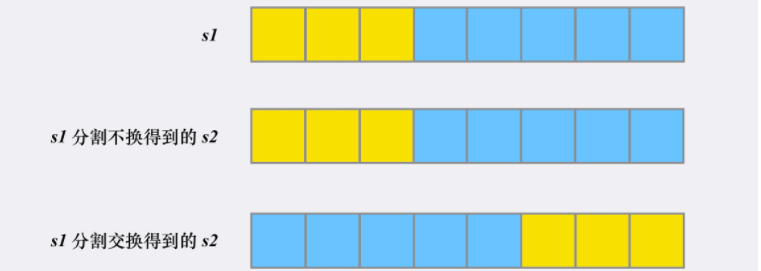
\includegraphics[width=.9\linewidth]{./pic/isScramble.png}


因为对于某个确定的分割点,s1s1 固定分为两部分,分别为 [0,i)[0,i) \& [i, n)[i,n)。

而 s2s2 可能会有两种分割方式,分别 [0,i)[0,i) \& [i,n)[i,n) 和 [0, n-i)[0,n−i) \& [n-i,n)[n−i,n)。

我们只需要递归调用 isScrambleisScramble 检查 s1s1 的 [0,i)[0,i) \& [i, n)[i,n) 部分能否与 「s2s2 的 [0,i)[0,i) \& [i,n)[i,n)」 或者 「s2s2 的 [0, n-i)[0,n−i) \& [n-i,n)[n−i,n)」 匹配即可。

同时,我们将「s1s1 和 s2s2 相等」和「s1s1 和 s2s2 词频不同」作为「递归」出口。

理解这套做法十分重要,后续的解法都是基于此解法演变过来。
\begin{minted}[fontsize=\scriptsize,linenos=false]{csharp}
private boolean idCheck(String ss, String tt) {
    int [] one = new int [26];
    int [] two = new int [26];
    char [] s = ss.toCharArray();
    char [] t = tt.toCharArray();
    for (int i = 0; i < s.length; i++) 
        one[s[i] - 'a']++;
    for (int i = 0; i < t.length; i++) 
        two[t[i]-'a']++;
    for (int i = 0; i < 26; i++) 
        if (one[i] != two[i])
            return false;
    return true;
}
public boolean isScramble(String s, String t) { // tle tle tle
    int n = s.length();
    if (n == 1) return s.charAt(0) == t.charAt(0);
    if (s.equals(t)) return true;
    if (!idCheck(s, t)) return false;
    for (int i = 1; i < n; i++) {
        System.out.println("\n i: " + i);
        String ls = s.substring(0, i), rs = s.substring(i);
        String ltone = t.substring(0, i), rtone = t.substring(i);
        String lttwo = t.substring(0, n-i), rttwo = t.substring(n-i);
        if (isScramble(ls, ltone) && isScramble(rs, rtone)
            || isScramble(ls, rttwo) && isScramble(rs, lttwo))
            return true;
    }
    return false;
}
\end{minted}

时间复杂度:O(5\^{}n)

空间复杂度:忽略递归与生成子串带来的空间开销,复杂度为 O(1)

\item 记忆化搜索
\label{sec-2-0-2-2}
朴素解法卡在了 286 / 288个样例。

我们考虑在朴素解法的基础上,增加「记忆化搜索」功能。

我们可以重新设计我们的「爆搜」逻辑:假设 s1 从 i 位置开始,s2 从 j 位置开始,后面的长度为 len 的字符串是否能形成「扰乱字符串」(互为翻转)。

那么在单次处理中,我们可分割的点的范围为 [1, len),然后和「递归」一下,将 s1 分割出来的部分尝试去和 s2 的对应位置匹配。

同样的,我们将「入参对应的子串相等」和「入参对应的子串词频不同」作为「递归」出口。
\begin{minted}[fontsize=\scriptsize,linenos=false]{csharp}
private boolean idCheck(String ss, String tt) {
    int [] one = new int [26];
    int [] two = new int [26];
    char [] s = ss.toCharArray();
    char [] t = tt.toCharArray();
    for (int i = 0; i < s.length; i++) 
        one[s[i] - 'a']++;
    for (int i = 0; i < t.length; i++) 
        two[t[i]-'a']++;
    for (int i = 0; i < 26; i++) 
        if (one[i] != two[i])
            return false;
    return true;
}
private int dfs(int i, int j, int k) { // k: length dp[i][j][len]: 这个dp的设计还是比较难想的!
    if (dp[i][j][k] != 0) return dp[i][j][k];
    String a = s.substring(i, i+k), b = t.substring(j, j+k);
    if (a.equals(b)) return dp[i][j][k] = 1;
    if (!idCheck(a, b)) return dp[i][j][k] = -1;
    for (int l = 1; l < k; l++) {
        if (dfs(i, j, l) == 1 && dfs(i+l, j+l, k-l) == 1)
            return dp[i][j][k] = 1;
        if (dfs(i, j+k-l, l) == 1 && dfs(i+l, j, k-l) == 1)
            return dp[i][j][k] = 1;
    }
    return dp[i][j][k] = -1;
}
int [][][] dp;
String s, t;
int n;
public boolean isScramble(String s, String t) {
    this.s = s;
    this.t = t;
    n = s.length();
    if (s.equals(t)) return true;
    if (!idCheck(s, t)) return false;
    dp = new int [n][n][n+1];
    return dfs(0, 0, s.length()) == 1;
}
\end{minted}
\item 动态规划(区间 DP)
\label{sec-2-0-2-3}
当然,这道题也可以用动态规划 Dynamic Programming,根据以往的经验来说,根字符串有关的题十有八九可以用 DP 来做,那么难点就在于如何找出状态转移方程。

其实有了上述「记忆化搜索」方案之后,我们就已经可以直接忽略原问题,将其改成「动态规划」了。

根据「dfs 方法的几个可变入参」作为「状态定义的几个维度」,根据「dfs 方法的返回值」作为「具体的状态值」。

我们可以得到状态定义 f[i][j][len]f[i][j][len]:

f[i][j][len]f[i][j][len] 代表 s1s1 从 ii 开始,s2s2 从 jj 开始,后面长度为 lenlen 的字符是否能形成「扰乱字符串」(互为翻转)。

状态转移方程其实就是翻译我们「记忆化搜索」中的 dfs 主要逻辑部分:

\begin{minted}[fontsize=\scriptsize,linenos=false]{csharp}
    // 对应了「s1 的 [0,i) & [i,n)」匹配「s2 的 [0,i) & [i,n)」
    if (dfs(i, j, k) && dfs(i + k, j + k, len - k)) {
        cache[i][j][len] = Y;
        return true;
    }
    // 对应了「s1 的 [0,i) & [i,n)」匹配「s2 的 [n-i,n) & [0,n-i)」
    if (dfs(i, j + len - k, k) && dfs(i + k, j, len - k)) {
        cache[i][j][len] = Y;
        return true;
    }
\end{minted}

从状态定义上,我们就不难发现这是一个「区间 DP」问题,区间长度大的状态值可以由区间长度小的状态值递推而来。

而且由于本身我们在「记忆化搜索」里面就是从小到大枚举 lenlen,因此这里也需要先将 len 这层循环提前,确保我们转移 f[i][j][len] 时所需要的状态都已经被计算好。

这道题看起来是比较复杂的,如果用brute force,每次做切割,然后递归求解,是一个非多项式的复杂度,一般来说这不是面试官想要的答案。

这其实是一道三维动态规划的题目,我们提出维护量res[i][j][n],其中i是s1的起始字符,j是s2的起始字符,而n是当前的字符串长度,res[i][j][len]表示的是以i和j分别为s1和s2起点的长度为len的字符串是不是互为scramble。

有了维护量我们接下来看看递推式,也就是怎么根据历史信息来得到res[i][j][len]。判断这个是不是满足,其实我们首先是把当前s1[i\ldots{}i+len-1]字符串劈一刀分成两部分,然后分两种情况:

第一种是左边和s2[j\ldots{}j+len-1]左边部分是不是scramble,以及右边和s2[j\ldots{}j+len-1]右边部分是不是scramble;

第二种情况是左边和s2[j\ldots{}j+len-1]右边部分是不是scramble,以及右边和s2[j\ldots{}j+len-1]左边部分是不是scramble。

如果以上两种情况有一种成立,说明s1[i\ldots{}i+len-1]和s2[j\ldots{}j+len-1]是scramble的。而对于判断这些左右部分是不是scramble我们是有历史信息的,因为长度小于n的所有情况我们都在前面求解过了(也就是长度是最外层循环)。

上面说的是劈一刀的情况,对于s1[i\ldots{}i+len-1]我们有len-1种劈法,在这些劈法中只要有一种成立,那么两个串就是scramble的。

总结起来递推式是res[i][j][len] = || (res[i][j][k] \&\& res[i+k][j+k][len-k] || res[i][j+len-k][k] \&\& res[i+k][j][len-k]) 对于所有1<=k<len,也就是对于所有len-1种劈法的结果求或运算。因为信息都是计算过的,对于每种劈法只需要常量操作即可完成,因此求解递推式是需要O(len)(因为len-1种劈法)。

如此总时间复杂度因为是三维动态规划,需要三层循环,加上每一步需要线行时间求解递推式,所以是O(n\^{}4)。虽然已经比较高了,但是至少不是指数量级的,动态规划还是有很大有事的,空间复杂度是O(n\^{}3)。

时间复杂度:O(n\^{}4)

空间复杂度:O(n\^{}3)

\begin{minted}[fontsize=\scriptsize,linenos=false]{csharp}
public boolean isScramble(String s, String t) {
    int n = s.length();
    if (s.equals(t)) return true;
    boolean [][][] dp = new boolean [n][n][n+1];
    for (int len = 1; len <= n; len++) 
        for (int i = 0; i+len <= n; i++) 
            for (int j = 0; j+len <= n; j++) {
                if (len == 1) {
                    dp[i][j][len] = s.charAt(i) == t.charAt(j);
                    continue;
                }
                for (int k = 1; k < len; k++) 
                    if (dp[i][j][k] && dp[i+k][j+k][len-k] || dp[i][j+len-k][k] && dp[i+k][j][len-k])
                        dp[i][j][len] = true;
            }
    return dp[0][0][n];
}
\end{minted}
\end{enumerate}

\subsection{2065. Maximum Path Quality of a Graph - Hard 记忆化搜索+ 重复遍历}
\label{sec-2-0-3}
There is an undirected graph with n nodes numbered from 0 to n - 1 (inclusive). You are given a 0-indexed integer array values where values[i] is the value of the ith node. You are also given a 0-indexed 2D integer array edges, where each edges[j] = [uj, vj, timej] indicates that there is an undirected edge between the nodes uj and vj, and it takes timej seconds to travel between the two nodes. Finally, you are given an integer maxTime.

A valid path in the graph is any path that starts at node 0, ends at node 0, and takes at most maxTime seconds to complete. You may visit the same node multiple times. The quality of a valid path is the sum of the values of the unique nodes visited in the path (each node's value is added at most once to the sum).

Return the maximum quality of a valid path.

Note: There are at most four edges connected to each node.
\begin{enumerate}
\item 解题思路与分析
\label{sec-2-0-3-0-1}

A straightforward idea is to try all paths from node 0 and calculate the max path quality for paths also end with node 0.

One \textbf{optimization} we can add is: once we cannot return back to node 0, we stop. The min\_time required from any node to node 0 can be pre-computed using Dijkstra algorithm.

\textbf{Time complexity:} O(4\^{}10)

\textbf{Note the constraints:} 10 <= time\_j, maxTime <= 100 and There are at most four edges connected to each node..

It means the max levels of dfs search is 10, and at each level we have maximum of 4 neighbouring nodes to try.

So the time complexity is: O(4\^{}10).

\begin{minted}[fontsize=\scriptsize,linenos=false]{csharp}
private int [] dijkstra() {
    int [] ans = new int [n];
    Arrays.fill(ans, Integer.MAX_VALUE);
    ans[0] = 0;
    // boolean [] vis = new boolean [n]; // 因为可以重复遍历,要允许它重复遍历  
    // vis[idx] = true;                  // 因为可以重复遍历,要允许它重复遍历  
    // Queue<int []> q = new LinkedList<>();
    Queue<int []> q = new PriorityQueue<>((a, b)->a[1] - b[1]);
    q.offer(new int [] {0, 0});
    while (!q.isEmpty()) {
        int [] cur = q.poll();
        if (cur[1] > ans[cur[0]]) continue;
        for (int [] nei : adj.get(cur[0])) 
            // if (nei[0] == cur[0]) continue; // 因为可以重复遍历,要允许它重复遍历  
            if (nei[1] + cur[1] < ans[nei[0]]) {
                ans[nei[0]] = nei[1] + cur[1];
                // if (!vis[nei[0]]) {
                q.offer(new int [] {nei[0], ans[nei[0]]});
                // vis[nei[0]] = true;
            }
    }
    return ans;
}
private void dfs(int idx, int avaTime, int [] t, int [] v, Set<Integer> vis) {
    if (idx == 0) {
        int cur = 0;
        for (Integer node : vis) 
            cur += v[node];
        ans = Math.max(ans, cur);
    }
    for (int [] nei : adj.get(idx)) 
        if (t[nei[0]] + nei[1] <= avaTime) { //
            boolean added = vis.add(nei[0]);
            dfs(nei[0], avaTime - nei[1], t, v, vis);
            if (added)
                vis.remove(nei[0]);
        }
}
int [] time;
List<List<int []>> adj = new ArrayList<>();
int n, ans = 0;
public int maximalPathQuality(int[] values, int[][] edges, int maxTime) {
    n = values.length;
    for (int i = 0; i < n; i++) 
        adj.add(new ArrayList<>());
    for (int [] e : edges) {
        adj.get(e[0]).add(new int [] {e[1], e[2]});
        adj.get(e[1]).add(new int [] {e[0], e[2]});
    }
    time = dijkstra();
    Set<Integer> si = new HashSet<>();
    si.add(0);
    dfs(0, maxTime, time, values, si);
    return ans;
}
\end{minted}
\end{enumerate}

\subsection{1397. Find All Good Strings - Hard 记忆化搜索}
\label{sec-2-0-4}
Given the strings s1 and s2 of size n and the string evil, return the number of good strings.

A good string has size n, it is alphabetically greater than or equal to s1, it is alphabetically smaller than or equal to s2, and it does not contain the string evil as a substring. Since the answer can be a huge number, return this modulo 109 + 7.
\begin{enumerate}
\item 解题思路与分析: 记忆化搜索
\label{sec-2-0-4-0-1}

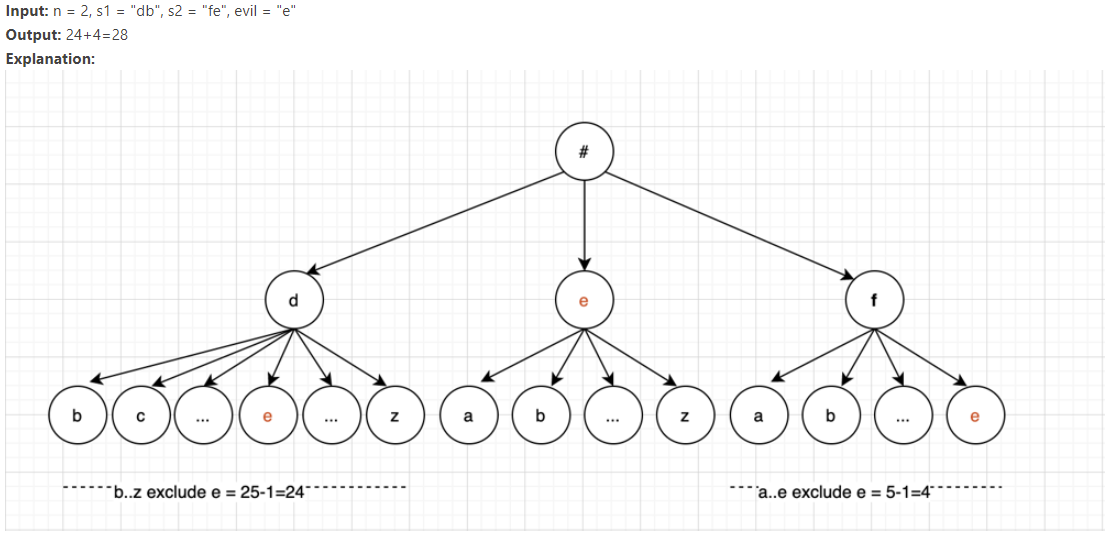
\includegraphics[width=.9\linewidth]{./pic/goodString.png}

\begin{itemize}
\item Complexity
\end{itemize}

Time: O(n*m*2*2*26), where n<=500, m<=50 is length of evil

Space: O(m*n*2*2)

\begin{minted}[fontsize=\scriptsize,linenos=false]{csharp}
private int [] computeLongestPrefixSuffix (char [] s) { // 这个要再理解一下: 重中之重
    int n = s.length;
    int [] lps = new int [n];
    for (int i = 1, j = 0; i < n; i++) {
        while (j > 0 && s[i] != s[j]) j = lps[j-1];  // 转向它 j 的前一位字符(在 j-1 下标)所指向的匹配位置 lps[j-1]
        if (s[i] == s[j]) lps[i] = ++j; // 同时增加两个的下标     
    }
    return lps;
}
private int getKey(int i, int j, boolean l, boolean r) { // bits occupied: i 9, j 6, l 1, r 1
    // 9 bits store n (2^9=512), 6 bits for m (2^6=64), 1 bit ro b1, 1 bit for b2
    return (i << 8) | (j << 2) | ((l ? 1 : 0) << 1) | (r ? 1 : 0); // 这是一个压缩空间存key的聪明技巧
} 
private int dfs(int n, int i, int evilMatched, boolean leftBound, boolean rightBound) {
    if (evilMatched == e.length) return 0; // matched evil string, no good
    if (i == n) return 1;                  // DIDN'T match evil string, great
    int key = getKey(i, evilMatched, leftBound, rightBound); // state: represented by <= 17 bits integer
    if (dp[key] > 0) return dp[key];
    char from = leftBound ? s[i] : 'a';
    char to = rightBound ? t[i] : 'z';
    int ans = 0;
    for (char c = from; c <= to; c++) { 
        int j = evilMatched; // j means the next match between current string (end at char `c`) and `evil` string
        while (j > 0 && e[j] != c) j = lps[j-1]; // 向左回塑寻找match字符c的上一个位置 ?
        if (c == e[j]) j++;
        ans += dfs(n, i+1, j, leftBound && (c == from), rightBound && (c == to));
        ans %= mod;
    }
    return dp[key] = ans;
}
int mod = (int)1e9 + 7;
char [] s, t, e;
int [] dp, lps;
public int findGoodStrings(int n, String s1, String s2, String evil) {
    dp = new int [1 << 17]; // Need total 17 bits, according to data limits
    s = s1.toCharArray();
    t = s2.toCharArray();
    e = evil.toCharArray();
    lps = computeLongestPrefixSuffix(e);
    return dfs(n, 0, 0, true, true);
}
\end{minted}
\item 动态规划: 数位DP + KMP todo: 改天把这个补上
\label{sec-2-0-4-1}
\begin{itemize}
\item \url{https://leetcode-cn.com/problems/find-all-good-strings/solution/shu-wei-dp-kmp-by-qodjf/}
\item \url{https://www.cnblogs.com/wenruo/p/12616985.html}
\item \url{https://www.codeleading.com/article/42703213478/}
\item \url{https://leetcode-cn.com/problems/find-all-good-strings/solution/shu-wei-dp-kmpqian-zhui-shu-zu-java-by-henrylee4/}
\item \url{https://leetcode-cn.com/problems/find-all-good-strings/solution/kmpshang-de-dpc-by-zhu-mang-4/}
\end{itemize}

之前做的题大部分是关于数字的数位dp,而现在要的就是字符串的数位dp。

设d p [ p o s ] [ s t a t s ] [ b o u n d ] dp[pos][stats][bound]为数位dp的数组,其中 p o s pospos表示第pos个位置的字符总共有的数量,s t a t s表示的是匹配e v i l的状态,即能够匹配到e v i l 数组的位置。b o u n d 表示此时能够选择字符的范围,即当前字符选择的时候是否有限制。

对于b o u n d 我们用四个数字表示
\begin{minted}[fontsize=\scriptsize,linenos=false]{csharp}
0 00 表示此时的字符选择是没有限制的,即可以选择的范围为a ∼ z
1 11 表示此时的字符选择是有下限的,所以选择的范围是s 1 [ p o s ] ∼ z
2 22 表示此时的字符选择是有上限的,所以可以选择的范围是a ∼ s 2 [ p o s ]
3 33 表示此时的字符既有上限又有下限。这种情况只有当s 1 [ p o s ] ∼ s 2 [ p o s ]
\end{minted}

而对于stats表示匹配e v i l evilevil字符的状态,由于e v i l evilevil的长度最长为50,所以可以生成字符串e v i l evilevil的next数组。那么当匹配不成立的时候,就可以直接进行跳转。

设一个记忆数组mem[e\_pos][n\_char]表示当匹配e v i l evilevil的位置为e\_pos时,下一个字符为n\_char时,可以跳转的位置,因为在整个搜索的过程中,可能需要多次调用这个数组,而这个数组大小为mem$\backslash$footnote\{DEFINITION NOT FOUND.\}$\backslash$textsuperscript\{,\}$\backslash$,\footnote\{DEFINITION NOT FOUND.\},因此没必要每次都计算。

对于如何生成next的数组,小伙伴们可以去搜索与K M P KMPKMP算法相关的博客查看。
\end{enumerate}

\subsection{2060. Check if an Original String Exists Given Two Encoded Strings - Hard dfs记忆化搜索}
\label{sec-2-0-5}
An original string, consisting of lowercase English letters, can be encoded by the following steps:

Arbitrarily split it into a sequence of some number of non-empty substrings.
Arbitrarily choose some elements (possibly none) of the sequence, and replace each with its length (as a numeric string).
Concatenate the sequence as the encoded string.
For example, one way to encode an original string "abcdefghijklmnop" might be:

Split it as a sequence: ["ab", "cdefghijklmn", "o", "p"].
Choose the second and third elements to be replaced by their lengths, respectively. The sequence becomes ["ab", "12", "1", "p"].
Concatenate the elements of the sequence to get the encoded string: "ab121p".
Given two encoded strings s1 and s2, consisting of lowercase English letters and digits 1-9 (inclusive), return true if there exists an original string that could be encoded as both s1 and s2. Otherwise, return false.

Note: The test cases are generated such that the number of consecutive digits in s1 and s2 does not exceed 3.
\begin{enumerate}
\item 解题思路与分析- (这里需要再好好总结一下)
\label{sec-2-0-5-1}
\begin{itemize}
\item solution is straight forward we have 2 pointer in each string
\end{itemize}
\begin{minted}[fontsize=\scriptsize,linenos=false]{csharp}
1.consider the easy case, they all character, we compare s1.charAt(i) == s2.charAt(j)
2.digit case, we get a number from s1, we can calculate the number s1 has, (descripton said less than 1000), 
  we can pass this value compare with number from s2 name it diff
3.character case if we still has remaing diff to spend passed from our parents, 
  so we can use one dollor a day, one diff one position dfs(i + 1, j, diff - 1
4.terminating condition, if both reach the end and diff == 0
\end{minted}

\begin{minted}[fontsize=\scriptsize,linenos=false]{csharp}
public boolean possiblyEquals(String ss, String tt) {
    m = ss.length(); N = 1000;
    n = tt.length();
    s = ss.toCharArray();
    t = tt.toCharArray();
    dp = new Boolean [m+1][n+1][2001]; // dp[i][j][diff] means if s1[i:] truncated by <diff> characters if diff > 0 
    return dfs(0, 0, 0);               // and s2[j:] truncated by <-diff> characters if diff < 0 are equal
}
Boolean [][][] dp;
char [] s, t;
int m, n, N;
private boolean dfs(int i, int j, int k) { // k: dif
    if (i == m && j == n) return k == 0;
    if (dp[i][j][k+N] != null) return dp[i][j][k+N];
    if (i < m && j < n && k == 0 && s[i] == t[j] && dfs(i+1, j+1, 0))   // Literal matching on s1[i] and s2[j]
        return dp[i][j][N] = true;
    if (i < m && !Character.isDigit(s[i]) && k > 0 && dfs(i+1, j, k-1)) // Literal matching on s1[i]
        return dp[i][j][k+N] = true;
    if (j < n && !Character.isDigit(t[j]) && k < 0 && dfs(i, j+1, k+1)) // Literal matching on s2[j]
        return dp[i][j][k+N] = true;
    for (int x = i, val = 0; x < m && Character.isDigit(s[x]); x++) {   // Wildcard matching on s1[i]
        val = val * 10 + s[x] - '0';
        if (dfs(x+1, j, k-val)) return dp[i][j][k+N] = true;
    }
    for (int x = j, val = 0; x < n && Character.isDigit(t[x]); x++) {   // Wildcard matching on s2[j]
        val = val * 10 + t[x] - '0';
        if (dfs(i, x+1, k+val)) return dp[i][j][k+N] = true;
    }
    return dp[i][j][k+N] = false;
}
\end{minted}
\end{enumerate}

\subsection{638. Shopping Offers - Medium 记忆化搜索 or 背包动态规划}
\label{sec-2-0-6}
In LeetCode Store, there are n items to sell. Each item has a price. However, there are some special offers, and a special offer consists of one or more different kinds of items with a sale price.

You are given an integer array price where price[i] is the price of the ith item, and an integer array needs where needs[i] is the number of pieces of the ith item you want to buy.

You are also given an array special where special[i] is of size n + 1 where special[i][j] is the number of pieces of the jth item in the ith offer and special[i][n] (i.e., the last integer in the array) is the price of the ith offer.

Return the lowest price you have to pay for exactly certain items as given, where you could make optimal use of the special offers. You are not allowed to buy more items than you want, even if that would lower the overall price. You could use any of the special offers as many times as you want.
\begin{enumerate}
\item 解题思路与分析: 记忆化搜索 List作key
\label{sec-2-0-6-1}
\begin{minted}[fontsize=\scriptsize,linenos=false]{csharp}
// 在java里,List的哈希方式,是将其哈希成开头加个1后的31进制整数,例如对于列表[ 1 , 2 , 3 ],java会将其哈希成31进制下的1123,也就是哈希成
// 1*31^3 + 1 * 32^2 + 2 * 31 + 3 = 30817,而List里判断是否equals,是逐个比较列表里的值,如果值全相等就返回true。
//     所以在记忆化的时候,可以直接把key设为是List类型的。
public int shoppingOffers(List<Integer> p, List<List<Integer>> of, List<Integer> need) {
    n = p.size();
    return dfs(p, of, need);
}
Map<List<Integer>, Integer> dp = new HashMap<>();
int n;
private int dfs(List<Integer> p, List<List<Integer>> of, List<Integer> need) {
    if (dp.containsKey(need)) return dp.get(need);  // 首先检查记忆
    int ans = 0;
    for (int i = 0; i < n; i++) 
        ans += p.get(i) * need.get(i);
    if (ans == 0) return ans; // ? 这里就不需要记忆了?
    for (List<Integer> cur : of) {
        if (cur.get(cur.size()-1) >= ans) continue; // >=
        List<Integer> newNeed = new ArrayList<>();
        for (int i = 0; i < n; i++) {
            if (cur.get(i) > need.get(i)) break;
            newNeed.add(need.get(i) - cur.get(i));
        }
        if (newNeed.size() == need.size()) // 即当前礼包合法
            ans = Math.min(ans, cur.get(cur.size()-1) + dfs(p, of, newNeed));
    }
    dp.put(need, ans);
    return ans;
}
\end{minted}
\item 解题思路与分析: 背包动态规划 todo bug fix
\label{sec-2-0-6-2}

当然此题也可以用背包的递推公式来做记忆化搜索,并且使用状态压缩记录每个物品有多少个。由于最多有6 66种物品,每个物品最多6 66个,所以可以用个6 × 3 6\texttimes{} 36×3位二进制数来表示每个物品有多少个。

\begin{minted}[fontsize=\scriptsize,linenos=false]{csharp}
public int shoppingOffers(List<Integer> price, List<List<Integer>> special, List<Integer> needs) { // todo: rest 6 test cases bug to be fixed
    n = price.size();
    int[][] dp = new int[special.size() + 1][1 << (n * 3)]; // 开一个记忆化数组,dp[i][s]表示如果只考虑前i个套餐的话,要买到s这个状态,至少需要多少花费
    System.out.println("(1 << n*3): " + (1 << n*3));
    for (int [] row : dp) Arrays.fill(row, -1); // 先初始化为-1
    int target = 0; // 求一下needs代表的状态,这里target的最低3位表示的是下标是0的商品要买多少个,以此类推
    for (int i = needs.size() - 1; i >= 0; i--) 
        target = (target << 3) + needs.get(i);
    System.out.println("Integer.toBinaryString(target): " + Integer.toBinaryString(target));
    return dfs(special.size(), target, special, price, dp);
}
int n;
// 返回的是,如果只考虑前count个套餐的话,要达到state这个状态的最小花费(当然单买也是考虑的)
private int dfs(int count, int state, List<List<Integer>> special, List<Integer> price, int[][] dp) {
    // System.out.println("state: " + state);
    // if (state >= (1 << n*3)) return 0;
    if (dp[count][state] != -1) return dp[count][state]; // 如果之前已经算出来过,则直接返回
    if (count == 0) { // 如果一个套餐都不考虑,那就是全单买
        dp[count][state] = 0;
        // 求一下每个商品买多少个,然后累加一下花费
        for (int i = 0; i < n; i++) {
            int c = state >> i * 3 & 7;
            dp[count][state] += c * price.get(i);
        }
        return dp[count][state];
    }
    dp[count][state] = dfs(count - 1, state, special, price, dp); // 考虑不选第count个套餐的情况
    List<Integer> sp = special.get(count - 1);                    // 考虑选第count个套餐的情况
    int nextState = 0; // 存一下考虑完当前套餐后的需求状态
    for (int i = n - 1; i >= 0; i--) { // 逆序遍历是为了方便nextState的计算
        int c = state >> i * 3 & 7;
        // System.out.println("c: " + c);
        if (c < sp.get(i)) { // 小了,说明当前套餐是不能选的,标记为-1并退出循环
            nextState = -1;
            break;
        }
        // System.out.println("(c - sp.get(i)): " + (c - sp.get(i)));
        nextState = (nextState << 3) + c - sp.get(i);
        // System.out.println("Integer.toBinaryString(nextState): " + Integer.toBinaryString(nextState));
    }
    if (nextState != -1)  // 如果当前套餐能选,再算一下选了当前套餐的情况下的最小花费
        dp[count][state] = Math.min(dp[count][state], sp.get(n) + dfs(count, nextState, special, price, dp));
    return dp[count][state];
}
\end{minted}
\end{enumerate}
\subsection{474. Ones and Zeroes - Medium}
\label{sec-2-0-7}
You are given an array of binary strings strs and two integers m and n.

Return the size of the largest subset of strs such that there are at most m 0's and n 1's in the subset.

A set x is a subset of a set y if all elements of x are also elements of y.
\begin{enumerate}
\item 解题思路与分析
\label{sec-2-0-7-1}
\begin{minted}[fontsize=\scriptsize,linenos=false]{csharp}
public int findMaxForm(String[] strs, int m, int p) { // m: 0 p: 1 dfs记忆化搜索
    n = strs.length;
    int [] one = new int [n]; // cnt 1s
    int [] two = new int [n]; // cnt 0s
    int cntOne = 0, cntZero = 0;
    for (int i = 0; i < n; i++) {
        String cur = strs[i];
        cntOne = 0;
        cntZero = 0;
        for (char c : cur.toCharArray()) {
            if (c == '0') cntZero++;
            else cntOne++;
        }
        one[i] = cntOne;
        two[i] = cntZero;
    }
    List<String> l = new ArrayList<>();
   cnt = new ArrayList<>();
    for (int i = 0; i < n; i++) {
        if (one[i] > p || two[i] > m) continue;
        l.add(strs[i]);
        cnt.add(new int [] {two[i], one[i]});
    }
    dp = new int [l.size()][m+1][p+1];
    return dfs(l, 0, m, p);
}
int [][][] dp;
List<int []> cnt;
int n;
private int dfs(List<String> l, int idx, int i, int j) { 
    if (idx >= l.size() || i < 0 || j < 0) return 0;
    if (i == 0 && j == 0) return 0;
    if (dp[idx][i][j] > 0) return dp[idx][i][j];
    int x = i - cnt.get(idx)[0], y = j - cnt.get(idx)[1];
    int ans = x >= 0 && y >= 0 ? 1 : 0;
    return dp[idx][i][j] = Math.max(ans + dfs(l, idx+1, x, y), dfs(l, idx+1, i, j));
 }
\end{minted}
\item 解题思路与分析: DP
\label{sec-2-0-7-2}

DP的写法要熟悉起来

\begin{minted}[fontsize=\scriptsize,linenos=false]{csharp}
public int findMaxForm(String[] strs, int m, int n) {
    int [][] dp = new int [m+1][n+1];
    dp[0][0] = 0;
    for (String s : strs) {
        int one = 0, zoo = 0;
        for (int i = 0; i < s.length(); i++) 
            if (s.charAt(i) == '0') ++ zoo;
            else ++one;
        for (int i = m; i >= zoo; i--) 
            for (int j = n; j >= one; j--) 
                dp[i][j] = Math.max(dp[i][j], dp[i-zoo][j-one] + 1);
    }
    return dp[m][n];
}
\end{minted}
\end{enumerate}
\subsection{1900. The Earliest and Latest Rounds Where Players Compete - Hard}
\label{sec-2-0-8}
There is a tournament where n players are participating. The players are standing in a single row and are numbered from 1 to n based on their initial standing position (player 1 is the first player in the row, player 2 is the second player in the row, etc.).

The tournament consists of multiple rounds (starting from round number 1). In each round, the ith player from the front of the row competes against the ith player from the end of the row, and the winner advances to the next round. When the number of players is odd for the current round, the player in the middle automatically advances to the next round.

For example, if the row consists of players 1, 2, 4, 6, 7
Player 1 competes against player 7.
Player 2 competes against player 6.
Player 4 automatically advances to the next round.
After each round is over, the winners are lined back up in the row based on the original ordering assigned to them initially (ascending order).

The players numbered firstPlayer and secondPlayer are the best in the tournament. They can win against any other player before they compete against each other. If any two other players compete against each other, either of them might win, and thus you may choose the outcome of this round.

Given the integers n, firstPlayer, and secondPlayer, return an integer array containing two values, the earliest possible round number and the latest possible round number in which these two players will compete against each other, respectively.
\begin{enumerate}
\item 解题思路与分析:分析本质不同的站位情况 + 记忆化搜索
\label{sec-2-0-8-1}

本题思维难度较大。其中的有些技巧可能在其它的题目中很少出现。

读者在第一次阅读本题解时,可以多去思考「怎么做」,而尽量不要去思考「为什么要这么做」。

\begin{enumerate}
\item 思路与算法
\label{sec-2-0-8-1-1}

我们可以用 F(n, f, s)F(n,f,s) 表示还剩余 nn 个人,并且两名最佳运动员分别是一排中从左往右数的第 ff 和 ss 名运动员时,他们比拼的最早回合数。

同理,我们用 G(n, f, s)G(n,f,s) 表示他们比拼的最晚回合数。

那么如何进行状态转移呢?

只考虑本质不同的站位情况

如果我们单纯地用 F(n, f, s)F(n,f,s) 来进行状态转移,会使得设计出的算法和编写出的代码都相当复杂。例如我们需要考虑 ff 是在左侧(即从前往后数)、中间(即轮空)还是右侧(即从后往前数),对于 ss 也需要考虑那么多情况,这样状态转移方程就相当麻烦。

我们可以考虑分析出本质不同的站位情况,得到下面的表格:
\begin{center}
\begin{tabular}{llll}
\hline
 & s 在左侧 & s 在中间 & s 在右侧\\
\hline
f 在左侧 & 保持不变 & 保持不变 & 保持不变\\
f 在中间 & 等价于「f 在左侧,s 在中间」 & 不存在这种情况 & 等价于「f 在左侧,s 在中间」\\
f 在右侧 & 等价于「f 在左侧,s 在右侧」 & 等价于「f 在左侧,s 在中间」 & 等价于「f 在左侧,s 在左侧」\\
\hline
\end{tabular}
\end{center}
其正确性在于:

\begin{itemize}
\item F(n, f, s) = F(n, s, f) 恒成立。即我们交换两名最佳运动员的位置,结果不会发生变化;
\item F(n, f, s) = F(n, n+1-s, n+1-f) 恒成立。因为我们会让从前往后数的第 ii 运动员与从后往前数的第 ii 名运动员进行比拼,那么我们将所有的运动员看成一个整体,整体翻转一下,结果同样不会发生变化。
\end{itemize}

我们使用这两条变换规则,就可以保证在 F(n, f, s)F(n,f,s) 中,ff 一定小于 ss,那么 ff 一定在左侧,而 ss 可以在左侧、中间或者右侧。这样我们就将原本的 88 种情况减少到了 33 种情况。

对于 G(n, f, s)G(n,f,s),其做法是完全相同的。

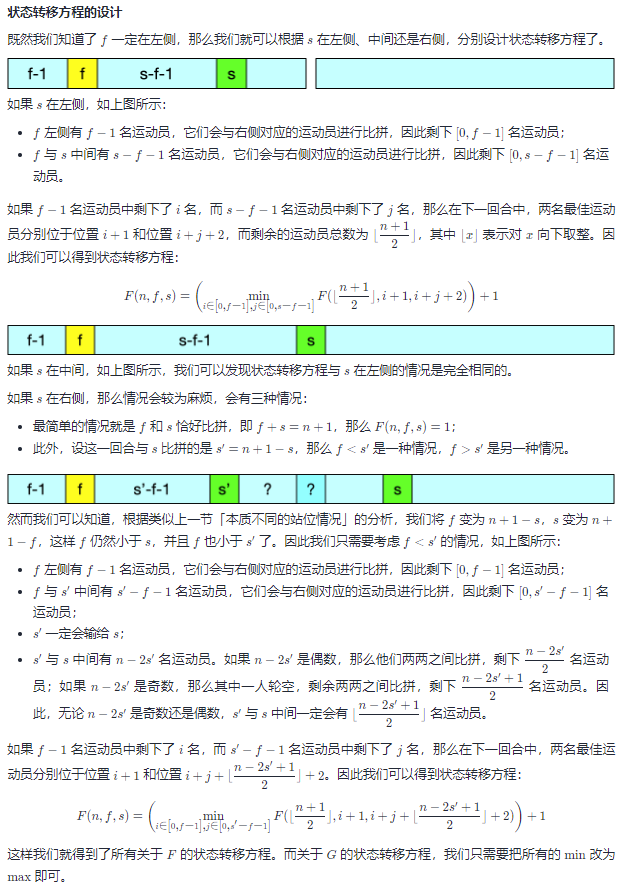
\includegraphics[width=.9\linewidth]{./pic/1900.png}

\item 细节
\label{sec-2-0-8-1-2}

在「本质不同的站位情况」一节中,我们提到了两种变换规则。那么我们具体应当在 n, f, s满足什么关系(而不是抽象的「左侧」「中间」「右侧」)时使用其中的哪些规则呢?

这里有很多种设计方法,我们介绍一种较为简单的,题解代码中使用的方法:

首先我们使用自顶向下的记忆化搜索代替动态规划进行状态转移,这样写更加简洁直观,并且无需考虑状态的求值顺序;

记忆化搜索的入口为 F(n,firstPlayer,secondPlayer)。我们在开始记忆化搜索之前,先通过变换规则 F(n,f,s)=F(n,s,f) 使得firstPlayer 一定小于 secondPlayer,这样一来,由于另一条变换规则 F(n,f,s)=F(n,n+1−s,n+1−f) 不会改变 ff 与 ss 间的大小关系,因此在接下来的记忆化搜索中,f<s 是恒成立的,我们也就无需使用变换规则 F(n,f,s)=F(n,s,f) 了;

在之前表格中,我们需要变换的情况有 55 种,分别是:「ff 在中间,ss 在左侧」「ff 在中间,ss 在右侧」「ff 在右侧,ss 在左侧」「ff 在右侧,ss 在中间」「ff 在右侧,ss 在右侧」。由于我们已经保证了 f < sf<s 恒成立,因此这 55 种情况中只剩下 22 种是需要处理的,即:「ff 在中间,ss 在右侧」和「ff 在右侧,ss 在右侧」。此外,我们在「状态转移方程的设计」一节中还发现了一种需要处理的情况,即「ff 在左侧,ss 在右侧,并且 f> s' =n+1−s」。

那么这 33 种情况是否可以统一呢?对于最后一种情况,我们有 f+s>n+1,而「ff 在中间,ss 在右侧」和「ff 在右侧,ss 在右侧」也恰好满足 f+s > n+1f+s>n+1,并且所有不需要变换的情况都不满足 f+s>n+1。因此我们只需要在 f+s>n+1 时,使用一次变换规则F(n,f,s)=F(n,n+1−s,n+1−f) 就行了。

\begin{minted}[fontsize=\scriptsize,linenos=false]{csharp}
// 3种情况是否可以统一呢?
// 对于最后一种情况,我们有 f+s > n+1f+s>n+1,
// 而「ff 在中间,ss 在右侧」和「ff 在右侧,ss 在右侧」也恰好满足 f+s > n+1f+s>n+1,
// 并且所有不需要变换的情况都不满足 f+s > n+1f+s>n+1。
// 因此我们只需要在 f+s > n+1 时,使用一次变换规则 F(n, f, s) = F(n, n+1-s, n+1-f) 就行
public int [] earliestAndLatest(int n, int firstPlayer, int secondPlayer) {
    min = new int [n+1][n+1][n+1];
    max = new int [n+1][n+1][n+1];
    if (firstPlayer < secondPlayer) return dfs(n, firstPlayer, secondPlayer);
    return dfs(n, secondPlayer, firstPlayer);
}
int [][][] min, max;
private int [] dfs(int n, int f, int s) { // f: firstPlayer, // s: secondPlayer
    if (min[n][f][s] > 0) return new int [] {min[n][f][s], max[n][f][s]};
    if (f + s == n+1) return new int [] {1, 1}; // 刚好第一轮就可以碰上
    if (f + s > n + 1) { // 三种特殊情况的变换:
        int [] res = dfs(n, n+1 - s, n+1 - f);
        min[n][f][s] = res[0];
        max[n][f][s] = res[1];
        return res;
    }
    int glbMin = Integer.MAX_VALUE, glbMax = 0;
    int half = (n+1) >> 1;
    if (s <= half) // // 在左侧或者中间
        for (int i = 0; i < f; i++) // f左侧人数
            for (int j = 0; j < s-f; j++) { // f和s之间的人数
                int [] res = dfs(half, i+1, i+j+2);
                glbMin = Math.min(glbMin, res[0]);
                glbMax = Math.max(glbMax, res[1]);
            }
    else {// s在右侧
        int s_prime = n + 1 - s;
        int mid = (n - 2 * s_prime + 1) / 2;
        for (int i = 0; i < f; i++) 
            for (int j = 0; j < s_prime - f; j++) { // s': n+1-s
                int [] res = dfs(half, i+1, i+j+2 + mid);
                // int [] res = dfs(half, i+1, i+j+2+(s*2-n-1)/2);
                glbMin = Math.min(glbMin, res[0]);
                glbMax = Math.max(glbMax, res[1]); 
            }
    }
    min[n][f][s] = glbMin + 1;
    max[n][f][s] = glbMax + 1;
    return new int [] {glbMin + 1, glbMax + 1};
}
\end{minted}
\end{enumerate}
\end{enumerate}
\subsection{488. Zuma Game - Hard}
\label{sec-2-0-9}
You are playing a variation of the game Zuma.

In this variation of Zuma, there is a single row of colored balls on a board, where each ball can be colored red 'R', yellow 'Y', blue 'B', green 'G', or white 'W'. You also have several colored balls in your hand.

Your goal is to clear all of the balls from the board. On each turn:

Pick any ball from your hand and insert it in between two balls in the row or on either end of the row.
If there is a group of three or more consecutive balls of the same color, remove the group of balls from the board.
If this removal causes more groups of three or more of the same color to form, then continue removing each group until there are none left.
If there are no more balls on the board, then you win the game.
Repeat this process until you either win or do not have any more balls in your hand.
Given a string board, representing the row of balls on the board, and a string hand, representing the balls in your hand, return the minimum number of balls you have to insert to clear all the balls from the board. If you cannot clear all the balls from the board using the balls in your hand, return -1.
\begin{enumerate}
\item 解题思路与分析: bfs广度优先搜索 todo
\label{sec-2-0-9-1}
\begin{minted}[fontsize=\scriptsize,linenos=false]{csharp}
public int findMinStep(String board, String hand) {
    char[] arr = hand.toCharArray();
    Arrays.sort(arr);
    hand = new String(arr);
    // 初始化用队列维护的状态队列:其中的三个元素分别为桌面球状态、手中球状态和回合数
    Queue<State> queue = new ArrayDeque<State>();
    queue.offer(new State(board, hand, 0));
    // 初始化用哈希集合维护的已访问过的状态
    Set<String> visited = new HashSet<String>();
    visited.add(board + " " + hand);
    while (!queue.isEmpty()) {
        State state = queue.poll();
        String curBoard = state.board;
        String curHand = state.hand;
        int step = state.step;
        for (int i = 0; i <= curBoard.length(); ++i) {
            for (int j = 0; j < curHand.length(); ++j) {
                // 第 1 个剪枝条件: 当前球的颜色和上一个球的颜色相同
                if (j > 0 && curHand.charAt(j) == curHand.charAt(j - 1)) 
                    continue;
                // 第 2 个剪枝条件: 只在连续相同颜色的球的开头位置插入新球
                if (i > 0 && curBoard.charAt(i - 1) == curHand.charAt(j)) 
                    continue;
                // 第 3 个剪枝条件: 只在以下两种情况放置新球
                boolean choose = false;
                //  - 第 1 种情况 : 当前球颜色与后面的球的颜色相同
                if (i < curBoard.length() && curBoard.charAt(i) == curHand.charAt(j)) 
                    choose = true;
                //  - 第 2 种情况 : 当前后颜色相同且与当前颜色不同时候放置球
                if (i > 0 && i < curBoard.length() && curBoard.charAt(i - 1) == curBoard.charAt(i) && curBoard.charAt(i - 1) != curHand.charAt(j))
                    choose = true;
                if (choose) {
                    String newBoard = clean(curBoard.substring(0, i) + curHand.charAt(j) + curBoard.substring(i));
                    String newHand = curHand.substring(0, j) + curHand.substring(j + 1);
                    if (newBoard.length() == 0) return step + 1;
                    String str = newBoard + " " + newHand;
                    if (visited.add(str)) 
                        queue.offer(new State(newBoard, newHand, step + 1));
                }
            }
        }
    }
    return -1;
}
public String clean(String s) {
    StringBuffer sb = new StringBuffer();
    Deque<Character> letterStack = new ArrayDeque<Character>();
    Deque<Integer> countStack = new ArrayDeque<Integer>();
    for (int i = 0; i < s.length(); ++i) {
        char c = s.charAt(i);
        while (!letterStack.isEmpty() && c != letterStack.peek() && countStack.peek() >= 3) {
            letterStack.pop();
            countStack.pop();
        }
        if (letterStack.isEmpty() || c != letterStack.peek()) {
            letterStack.push(c);
            countStack.push(1);
        } else countStack.push(countStack.pop() + 1);
    }
    if (!countStack.isEmpty() && countStack.peek() >= 3) {
        letterStack.pop();
        countStack.pop();
    }
    while (!letterStack.isEmpty()) {
        char letter = letterStack.pop();
        int count = countStack.pop();
        for (int i = 0; i < count; ++i) 
            sb.append(letter);
    }
    sb.reverse();
    return sb.toString();
}
class State {
    String board;
    String hand;
    int step;
    public State(String board, String hand, int step) {
        this.board = board;
        this.hand = hand;
        this.step = step;
    }
}
\end{minted}
\item 解题思路与分析: dfs记忆化搜索
\label{sec-2-0-9-2}
\begin{minted}[fontsize=\scriptsize,linenos=false]{csharp}
Map<String, Integer> dp = new HashMap<String, Integer>();
public int findMinStep(String b, String h) {
    char [] s = h.toCharArray();
    Arrays.sort(s);
    h = new String(s);
    int ans = dfs(b, h);
    return ans <= 5 ? ans : -1;
}
private int dfs(String b, String h) {
    if (b.length() == 0) return 0;
    String key = b + "_" + h;
    if (dp.containsKey(key)) return dp.get(key);
    int ans = 6;
    for (int j = 0; j < h.length(); j++) {
        if (j > 0 && h.charAt(j) == h.charAt(j - 1)) continue; // 第 1 个剪枝条件: 当前球的颜色和上一个球的颜色相同
        for (int i = 0; i <= b.length(); ++i) {
            if (i > 0 && b.charAt(i - 1) == h.charAt(j)) continue; // 第 2 个剪枝条件: 只在连续相同颜色的球的开头位置插入新球, 代码不懂 b[i] == b[i-1]?
            boolean choose = false; // 第 3 个剪枝条件: 只在以下两种情况放置新球
            //  - 第 1 种情况 : 当前球颜色与后面的球的颜色相同
            if (i < b.length() && b.charAt(i) == h.charAt(j)) 
                choose = true;
            //  - 第 2 种情况 : 当前后颜色相同且与当前颜色不同时候放置球 (在两个相同着色的中间放置不同着色的球?)
            if (i > 0 && i < b.length() && b.charAt(i - 1) == b.charAt(i) && b.charAt(i - 1) != h.charAt(j)) 
                choose = true;
            if (choose) {
                String newB = clean(b.substring(0, i) + h.charAt(j) + b.substring(i));
                String newH = h.substring(0, j) + h.substring(j + 1);
                ans = Math.min(ans, dfs(newB, newH) + 1);
            }
        }
    }
    dp.put(key, ans);
    return dp.get(key);
}
public String clean(String t) {
    Deque<Character> charSt = new ArrayDeque<Character>();
    Deque<Integer> cntSt = new ArrayDeque<Integer>();
    StringBuffer sb = new StringBuffer();
    char [] s = t.toCharArray();
    for (int i = 0; i < s.length; ++i) {
        char c = s[i];
        while (!charSt.isEmpty() && c != charSt.peek() && cntSt.peek() >= 3) { // 把能消除的先消除掉
            charSt.pop();
            cntSt.pop();
        }
        if (charSt.isEmpty() || c != charSt.peek()) { // 要么栈空了,要么字符不同,入栈(2个)
            charSt.push(c);
            cntSt.push(1); // 记数为1
        } else // 栈顶有相同的字符,但计数不够3,入栈,加数
            cntSt.push(cntSt.pop() + 1);
    }
    if (!cntSt.isEmpty() && cntSt.peek() >= 3) {
        charSt.pop();
        cntSt.pop();
    }
    while (!charSt.isEmpty()) {
        char letter = charSt.pop();
        int count = cntSt.pop();
        sb.append(String.valueOf(letter).repeat(count));
        // for (int i = 0; i < count; ++i) sb.append(letter);
    }
    sb.reverse();
    return sb.toString();
}
class St {
    String b, h;
    int cnt;
    public St(String bd, String hd, int cnt) {
        this.b = bd;
        this.h = hd;
        this.cnt = cnt;
    }
}
\end{minted}
\end{enumerate}

\chapter{Segment Tree与Binary Index Tree 线段树与树状数组}
\label{sec-3}

线段树(segment tree),顾名思义, 是用来存放给定区间(segment, or interval)内对应信息的一种数据结构。与树状数组(binary indexed tree)相似,线段树也用来处理数组相应的区间查询(range query)和元素更新(update)操作。与树状数组不同的是,线段树不止可以适用于区间求和的查询,也可以进行区间最大值,区间最小值(Range Minimum/Maximum Query problem)或者区间异或值的查询。

对应于树状数组,线段树进行更新(update)的操作为O(logn),进行区间查询(range query)的操作也为O(logn)。

\subsection{1157. Online Majority Element In Subarray - Hard}
\label{sec-3-0-1}
Design a data structure that efficiently finds the majority element of a given subarray.

The majority element of a subarray is an element that occurs threshold times or more in the subarray.

Implementing the MajorityChecker class:

MajorityChecker(int[] arr) Initializes the instance of the class with the given array arr.
int query(int left, int right, int threshold) returns the element in the subarray arr[left\ldots{}right] that occurs at least threshold times, or -1 if no such element exists.
\begin{enumerate}
\item 解题思路与分析
\label{sec-3-0-1-1}
\begin{itemize}
\item \url{https://www.cnblogs.com/slowbirdoflsh/p/11381565.html} 思路比较清晰
\end{itemize}

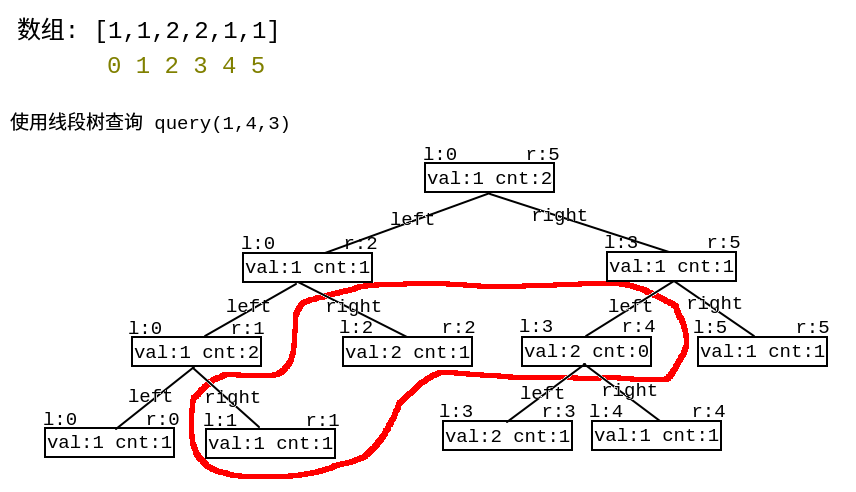
\includegraphics[width=.9\linewidth]{./pic/1157.png}

\begin{minted}[fontsize=\scriptsize,linenos=false]{csharp}
Map<Integer, List<Integer>> idx; // idx 存储数组出现元素种类 以及该元素下标索引
Node root; // 线段树的根节点
int key = 0, cnt = 0; // key 所查找的区域众数; count 所查找的区域众数出现次数, 
public MajorityChecker(int[] a) {
    idx = new HashMap<>(); // idx 存储数组出现元素种类 以及该元素下标索引
    for (int i = 0; i < a.length; i++)
        idx.computeIfAbsent(a[i], z -> new ArrayList<>()).add(i);
    root = buildTree(a, 0, a.length-1);
}
public int query(int left, int right, int threshold) {
    key = 0; cnt = 0; // 初始化 所查询众数key 及辅助判断的计数cnt
    searchTree(root, left, right); // 查询线段树
    // 如果查询区域没有众数 即key没被更改; 或者,
    // 所查询出来的众数 在原数组中根本没有超出阈值的能力
    if (key == 0 || idx.get(key).size() < threshold) return -1;
    // 上确界 排序数组中 第一个大于right的下标
    int r = upper_bound(idx.get(key), right);
    // 下确界 排序数组中 第一个大于等于left的下标
    int l = lower_bound(idx.get(key), left);
    cnt = r - l;
    return cnt >= threshold ? key : -1;
}
int upper_bound(List<Integer> list, int v) { // 排序数组中 第一个大于tar的下标
    int l = 0, r = list.size();
    while (l < r) {
        int mid = l + (r - l) / 2;
        if (list.get(mid) <= v) l = mid + 1;
        else r = mid;
    }
    return l;
}
int lower_bound(List<Integer> list, int v) { // 排序数组中 第一个大于等于tar的下标
    int l = 0, r = list.size();
    while (l < r) {
        int mid = l + (r - l) / 2;
        if (list.get(mid) < v) l = mid+1;
        else r = mid;
    }
    return l;
}
void searchTree(Node root, int l, int r) {
    if (root == null || l > r) return ;
    if (root.l > r || root.r < l) return ;
    if (root.l >= l && root.r <= r) { // 当查询边界被节点边界覆盖,该节点就是查询区域
        if (key == root.v) cnt += root.cnt;
        else if (cnt <= root.cnt) {
            key = root.v;
            cnt = root.cnt - cnt;
        } else cnt = cnt - root.cnt;
        return ;
    }
    int mid = (root.l + root.r) / 2; // 这两个查询条件再好好想想 !!!!!!!!!!!!!!!
    if (l <= mid)   // root.l <= l <= mid 左节点也可以是查询区域
        searchTree(root.left, l, r);
    if (r >= mid+1) // mid+1 <= r <= root.r 右节点也可以是查询区域
        searchTree(root.right, l, r);
}
Node buildTree(int [] a, int l, int r) {
    if (l > r) return null;
    Node root = new Node(l, r); // 初始一个线段树的根节点
    if (l == r) { // 叶子节点  
        root.v = a[l];
        root.cnt = 1;
        return root;
    }
    int mid = (l + r) / 2;
    root.left = buildTree(a, l, mid);
    root.right = buildTree(a, mid+1, r);
    makeRoot(root); // 整合父节点
    return root;
}
void makeRoot(Node r) { // 整合父节点
    if (r == null) return ;
    if (r.left != null) { // 如果该节点有左子节点 该节点的值"先"等于左子节点
        r.v = r.left.v;
        r.cnt = r.left.cnt;
    }
    if (r.right != null) { // 如果该节点还有右子节点 融合父节点和子节点
        if (r.v == r.right.v)
            r.cnt = r.cnt + r.right.cnt;
        else {
            if (r.cnt >= r.right.cnt)
                r.cnt = r.cnt - r.right.cnt;
            else {
                r.v = r.right.v;
                r.cnt = r.right.cnt - r.cnt;
            }
        }
    }
}
class Node {
    int l, r, v, cnt;
    Node left, right;
    public Node(int l, int r) {
        this.l = l; this.r = r;
        v = 0; cnt = 0;
        left = null; right = null;
    }
}
\end{minted}
\end{enumerate}

\subsection{1825. Finding MK Average - Hard}
\label{sec-3-0-2}
You are given two integers, m and k, and a stream of integers. You are tasked to implement a data structure that calculates the MKAverage for the stream.

The MKAverage can be calculated using these steps:

If the number of the elements in the stream is less than m you should consider the MKAverage to be -1. Otherwise, copy the last m elements of the stream to a separate container.
Remove the smallest k elements and the largest k elements from the container.
Calculate the average value for the rest of the elements rounded down to the nearest integer.
Implement the MKAverage class:

MKAverage(int m, int k) Initializes the MKAverage object with an empty stream and the two integers m and k.
void addElement(int num) Inserts a new element num into the stream.
int calculateMKAverage() Calculates and returns the MKAverage for the current stream rounded down to the nearest integer.
\begin{minted}[fontsize=\scriptsize,linenos=false]{csharp}
// 根据题意需要找到前k大的数,又需要求区间和,就自然想到线段树.写起来较不容易出错。
// 维护2个线段树数组,一个记录数的个数,一个记录区间值,
// 注意一般线段树中[s,e]指固定的区间,这里类似线段数求第k小的数,所以[s,e]指第s小的值到第e小的值的区间。
    Deque<Integer> q = new ArrayDeque<>(); // 始终维护m个数
    int [] cnt;  // 每个元素出现的次数
    long [] sum; // 累积和
    int m, k, n = 100000, N = n * 4 + 1; // 线段树所占用的空间为数组的四倍大小
    public MKAverage(int m, int k) {
        cnt = new int [N];
        sum = new long [N];
        this.m = m;
        this.k = k;
    }
    public void addElement(int num) {
        if (q.size() == m) {
            int v = q.pollFirst();
            insert(1, 0, n, v, -1); // 当删除掉一个元素的时候,需要更新线段树中的和
        }
        insert(1, 0, n, num, 1);
        q.offerLast(num);
    }
    public int calculateMKAverage() {
        if (q.size() < m) return -1;
        int bgn = k + 1, end = m - k; // idx: 1 - based
        return (int)(query(1, 0, n, bgn, end) / (m - 2 * k));
    }
    void insert(int idx, int l, int r, int v, long d) { // d: 
        cnt[idx] += d;
        sum[idx] += d * v;
        if (l == r) return ;
        int m = l + (r - l) / 2;
        if (v <= m)
            insert(idx << 1, l, m, v, d);       // 向左子树查询
        else insert(idx << 1 | 1, m+1, r, v, d);// 向右子树查询
    }
    long query(int idx, int l, int r, int bgn, int end) { // 线段中第 bgn 个到第 end 个
        if (l == r) { // 起始和结束最多出现2次此情况 ?
            int c = end - bgn + 1;
            return (long)c * l; //
        } else if (cnt[idx] == end - bgn + 1)
            return sum[idx];
        else {
            int m = l + (r - l) / 2;
            int cl = cnt[idx << 1];     // left child cnt
            // int cr = cnt[idx << 1 | 1];     // left child cnt
            if (cl >= end) // 搜索 左 子树
                return query(idx << 1, l, m, bgn, end); 
            else if (cl >= bgn) // 搜索 左 右 子树
                return query(idx << 1, l, m, bgn, cl) + query(idx << 1 | 1, m+1, r, 1, end - cl);
            else // cl < bgn, 搜索 右 子树
                return query(idx << 1 | 1, m+1, r, bgn - cl, end - cl);
        }
    }
\end{minted}
\begin{enumerate}
\item 解题思路与分析: 三个TreeMap, 自定义TreeMap
\label{sec-3-0-2-1}
\begin{minted}[fontsize=\scriptsize,linenos=false]{csharp}
    CusTreeMap [] ms;
    Deque<Integer> q;
    int m, k, n;
    public MKAverage(int m, int k) {
        this.m = m;
        this.k = k;
        q = new ArrayDeque<>();
        if (m - 2 * k > 0) {
            n = 3;
            ms = new CusTreeMap[n];
            ms[1] = new CusTreeMap(m - 2 * k);
        } else {
            n = 2;
            ms = new CusTreeMap[n];
        }
        ms[0] = new CusTreeMap(k);
        ms[n-1] = new CusTreeMap(k);
    }
    // 删除num,结果总是使mapList的小、中、大三个treemap依次填充。(先保证最小的treeMap填充、再保证中间的treeMap填充、最后是最大的填充)
    private void removeElement(int num) {
        boolean removed = false;
        for (int i = 0; i < n; i++) {
            if (!removed)
                removed = ms[i].remove(num);
            else { // 将后现一两个图中的最小元素向前一个图中挪动一个数值
                Integer minK = ms[i].pollFirst();
                if (minK == null) break;
                ms[i-1].add(minK);
            }
        }
    }
    public void addElement(int num) {
        if (q.size() == m) {
            int v = q.pollFirst();
            removeElement(v);
        }
        q.offerLast(num);
        Integer vtoAdd = num;
        for (int i = 0; i < n && vtoAdd != null; i++) 
            vtoAdd = ms[i].add(vtoAdd); // 记得这里返回的是: 如果图中已有k个元素,扔出来的最大键
    }
    public int calculateMKAverage() {
        if (q.size() < m || n < 3) return -1;
        return ms[1].avg();
    }
    class CusTreeMap {
        TreeMap<Integer, Integer> m;
        final int capacity;
        int size, sum;
        public CusTreeMap(int capacity) {
            m = new TreeMap<>();
            this.capacity = capacity;
        }
        public boolean remove(int key) {
            if (m.containsKey(key)) {
                m.put(key, m.get(key)-1);
                if (m.get(key) == 0) m.remove(key);
                sum -= key;
                size--;
                return true;
            }
            return false;
        }
        public Integer pollFirst() { // return key
            if (m.size() > 0) {
                int k = m.firstKey();
                // m.remove(k); // BUG: 你也不能用原始的TreeMap.remove(),因为它会移走所有的重复(如果这个元素存在重复的话)
                remove(k); // !!!
                return k;  // 这里没有自动更新 和 
                // return m.firstKey(); // BUG: 这里并没有真正移走这个元素,只是返回了第个元素的键
            }
            return null;
        }
        public Integer add(int key) { // 返回的是删除掉元素的键
            m.put(key, m.getOrDefault(key, 0) + 1); // 这里新填入的元素是否是最后一个元素,关系不大
            size++;
            sum += key;
            if (size > capacity) {
                int last = m.lastKey();
                m.put(last, m.get(last)-1);
                if (m.get(last) == 0) m.remove(last);
                sum -= last;
                size--;
                return last;
            }
            return null;
        }
        public int avg() {
            return sum / size;
        }
    }
\end{minted}
\item 解题思路与分析: 树状数组
\label{sec-3-0-2-2}
\begin{itemize}
\item 数状数组的解法: 另外第一次看到别人 二分+树状数组也能求前k大的值。
\end{itemize}
\begin{minted}[fontsize=\scriptsize,linenos=false]{csharp}
// We can have a queue to maintain m elements
// Use two Fenwick tree, 1 for count and 1 for prefix sum
// Do 2 times binary search for the first k elements and the last k elements by using the count from our first fenwick tree
// We can get the sum by subtrating the sum of first k elements and sum of last k element by using our second fenwick tree
Queue<Integer> q = new LinkedList<>();
FenWick fone, ftwo;
int [] cnt = new int [100010];
long sum = 0;
int m,k;
public MKAverage(int m, int k) {
    this.m = m;
    this.k = k;
    long A [] = new long [100010];
    long B [] = new long [100010];
    fone = new FenWick(A);
    ftwo = new FenWick(B);
}
public void addElement(int num) {
    q.add(num);
    sum += num;
    fone.update(num, 1);
    ftwo.update(num, num);
    cnt[num]++;
}
public int calculateMKAverage() {
    if (q.size() < m) return -1;
    while (q.size() > m) {
        int cur = q.poll();
        cnt[cur]--;
        sum -= cur;
        fone.update(cur, -1);
        ftwo.update(cur, -cur);
    }
    // binary search for the first k (there may be duplicated)
    int l = 0, r = cnt.length-1;
    int i = -1, j = -1; // pos1, pos2 
    while (l <= r) { // 二分查找总计数
        int m = (r + l) / 2;
        long count = fone.sumRange(0, m);
        if (count >= k) {
            i = m;
            r = m -1;
        } else l = m+1;
    }
    // binary search for the last k (there may be duplicated)
    l = 0;
    r = cnt.length-1;
    while (l <= r) {
        int m = l + (r-l)/2;
        long count = fone.sumRange(m, cnt.length-1);
        if (count >= k) {
            j = m;
            l = m + 1;
        } else r = m-1;
    }
    long sum1 = ftwo.sumRange(0,  i);
    long sum2 = ftwo.sumRange(j, cnt.length-1);
    long cnt1 = fone.sumRange(0, i);
    long cnt2 = fone.sumRange(j, cnt.length-1);
    if (cnt1 > k)
        sum1 -= i*(cnt1-k);
    if (cnt2 > k)
        sum2 -= j*(cnt2-k);
    long remain = sum - sum1 - sum2; // 总和, 减去两边最小最大各K个数的和
    return (int)(remain / (m-2*k));
}
class FenWick {
    long tree []; //1-index based
    long A [];
    long arr[];
    public FenWick(long [] A) {
        this.A = A;
        arr = new long [A.length];
        tree = new long [A.length + 1];
    }
    public void update(int i, int v) {
        arr[i] += v;
        i++;
        while (i < tree.length) {
            tree[i] += v;
            i += (i & -i); // 这是的原理细节再回去复习一下
        }
    }
    public long sumRange(int i, int j) {
        return pre(j+1)-pre(i);
    }
    public long pre(int i) {
        long sum = 0;
        while (i > 0) {
            sum += tree[i];
            i -= (i & -i);
        }
        return sum;
    }
}
\end{minted}
\begin{itemize}
\item 其它比较有兴趣以的BST二叉树的解法,改天补起来
\end{itemize}
\end{enumerate}
\subsection{315. Count of Smaller Numbers After Self - Hard}
\label{sec-3-0-3}
You are given an integer array nums and you have to return a new counts array. The counts array has the property where counts[i] is the number of smaller elements to the right of nums[i].
\begin{enumerate}
\item 解题思路与分析: 二分查找的插入排序
\label{sec-3-0-3-1}
\begin{minted}[fontsize=\scriptsize,linenos=false]{csharp}
public List<Integer> countSmaller(int[] a) { // O(NlogN) 插入排序
    int n = a.length;
    List<Integer> ans = new ArrayList<>();
    List<Integer> list = new ArrayList<>(); // 新建一个list,用于排序
    int [] tmp = new int [n]; // 为了提高效率,新建一个数组型的返回结果
    for (int i = n-1; i >= 0; i--) {
        int v = a[i];       // 将当前数字插入到新建list中, 使用二分查找找到插入位置
        int l = 0, r = list.size()-1; // l: left; r: right 从排好序的list中二分查找正确的插入位置
        while (l <= r) {
            int m = l + (r - l) / 2;
            if (v <= list.get(m)) r = m-1;
            else l = m + 1;
         }
        list.add(l, v); // 将当前数字插入到相应位置,保证list升序排列
        tmp[i] = l; // 当前位置前所有数字均小于当前数字,将个数加入返回结果
    }
    for (Integer v : tmp) ans.add(v);
    return ans;
}
\end{minted}
\item 解题思路与分析: 数状数组
\label{sec-3-0-3-2}
\begin{itemize}
\item 官方题解: \url{https://leetcode-cn.com/problems/count-of-smaller-numbers-after-self/solution/ji-suan-you-ce-xiao-yu-dang-qian-yuan-su-de-ge-s-7/}
\begin{minted}[fontsize=\scriptsize,linenos=false]{csharp}
private int[] c;
private int[] a; // 离散化、去重复 后的数组
public List<Integer> countSmaller(int[] nums) {
    List<Integer> ans = new ArrayList<Integer>(); 
    discretization(nums);
    init(nums.length + 5);
    for (int i = nums.length - 1; i >= 0; --i) {
        int id = getId(nums[i]);
        ans.add(query(id - 1));
        update(id);
    }
    Collections.reverse(ans);
    return ans;
}
private void init(int length) {
    c = new int[length];
    Arrays.fill(c, 0);
}
private int lowBit(int x) {
    return x & (-x);
}
private void update(int pos) {
    while (pos < c.length) {
        c[pos] += 1;
        pos += lowBit(pos);
    }
}
private int query(int pos) {
    int ret = 0;
    while (pos > 0) {
        ret += c[pos];
        pos -= lowBit(pos);
    }
    return ret;
}
private void discretization(int[] nums) { // 离散化、去重复 ?
    Set<Integer> set = new HashSet<Integer>(Arrays.stream(nums).boxed().collect(Collectors.toList()));
    int size = set.size();
    a = new int[size];
    int index = 0;
    for (int num : set) a[index++] = num;
    Arrays.sort(a);
}
private int getId(int x) {
    return Arrays.binarySearch(a, x) + 1; // 
}
\end{minted}
\end{itemize}
\item 解题思路与分析: 归并排序 todo 补上
\label{sec-3-0-3-3}
\end{enumerate}

\subsection{327. Count of Range Sum - Hard \textbf{重点} 这几个题要好好再理解消化几遍}
\label{sec-3-0-4}
Given an integer array nums and two integers lower and upper, return the number of range sums that lie in [lower, upper] inclusive.

Range sum S(i, j) is defined as the sum of the elements in nums between indices i and j inclusive, where i <= j.
\begin{enumerate}
\item 解题思路与分析: 分治法
\label{sec-3-0-4-1}

在累积和的基础上,我们计算有多少个区间的大小落在[lower, upper]之间,一个朴素的算法就是枚举各个区间,其时间复杂度是O(n\^{}2)。一个更好的方法是利用分治法来处理,即利用归并排序算法将数组分成左右两边,在合并左右数组之前,对于左边数组中的每一个元素,在右边数组找到一个范围,使得在这个范围中的元素与左边元素构成的区间和落在[lower, upper]之间,即在右边数组中找到两个边界,设为m,n,其中m是在右边数组中第一个使得sum[m] - sum[i] >= lower的位置,而n是第一个使得sum[n] - sum[i] > upper的位置,这样n-m就是与左边元素i所构成的位于[lower, upper]范围的区间个数。因为左右两边都是已经有序的,这样就可以避免不必要的比较(这也是为什么我们能将时间复杂度从O(n\^{}2)降低到O(nlogn)的秘诀所在)。

\begin{minted}[fontsize=\scriptsize,linenos=false]{csharp}
public int countRangeSum(int[] a, int lower, int upper) { // 这个merge sort的思维很奇特: 二分,O(NlogN)
    int n = a.length;
    long [] sum = new long[n+1];
    for (int i = 1; i <= n; i++) 
        sum[i] = sum[i-1] + a[i-1];
    return mergeAnalyse(sum, 0, n+1, lower, upper);
}
int mergeAnalyse(long [] a, int l, int r, int lo, int hi) { // l, r: 寻找[l, r)范围内和为[lower, upper]的片段的个数
    if (r - l <= 1) return 0;
    int mid = l + (r - l) / 2;
    int m = mid, n = mid, ans = 0;
    ans = mergeAnalyse(a, l, mid, lo, hi) + mergeAnalyse(a, mid, r, lo, hi);
    for (int i = l; i < mid; i++) { // 遍历[l, r)的半段长度: pivot 右移,滑动窗口,寻找合法窗口 // 通过遍历寻找当前范围中符合要求的个数,
        while (m < r && a[m] - a[i] < lo) m++; // 左端点右移,直到找到合法(sum >= lo)的解:m合法
        while (n < r && a[n] - a[i] <= hi) n++; // 右端点右移,直到右端点右移至不再合法(sum > hi), n 不合法 
        ans += n - m; // 对于[l, r)范围内的当前i来说,满足要求的总个数为 n - m
    }
    Arrays.sort(a, l, r); // 将[l, r)片段排序
    return ans;
}
\end{minted}
\item 解题思路与分析: 线段树
\label{sec-3-0-4-2}
\begin{itemize}
\item 官方题解:\url{https://leetcode-cn.com/problems/count-of-range-sum/solution/qu-jian-he-de-ge-shu-by-leetcode-solution/} 
\begin{minted}[fontsize=\scriptsize,linenos=false]{csharp}
public int countRangeSum(int[] a, int lo, int hi) {
    int n = a.length;
    long [] preSum = new long[n + 1];
    for (int i = 1; i <= n; i++) 
        preSum[i] = preSum[i-1] + a[i-1];
    Set<Long> allNumbers = new TreeSet<Long>();
    for (long x : preSum) {
        allNumbers.add(x);
        allNumbers.add(x - lo); //
        allNumbers.add(x - hi); // 
    }
    // 利用哈希表进行离散化
    Map<Long, Integer> values = new HashMap<Long, Integer>();
    int idx = 0;
    for (long x : allNumbers) {
        values.put(x, idx);
        idx++;
    }
    SegNode root = build(0, values.size() - 1);
    int ret = 0;
    for (long x : preSum) {
        int left = values.get(x - hi), right = values.get(x - lo);
        ret += count(root, left, right);
        insert(root, values.get(x));
    }
    return ret;
}
public SegNode build(int left, int right) {
    SegNode node = new SegNode(left, right);
    if (left == right) {
        return node;
    }
    int mid = (left + right) / 2;
    node.lchild = build(left, mid);
    node.rchild = build(mid + 1, right);
    return node;
}
public int count(SegNode root, int left, int right) {
    if (left > root.hi || right < root.lo) 
        return 0;
    if (left <= root.lo && root.hi <= right) 
        return root.add;
    return count(root.lchild, left, right) + count(root.rchild, left, right);
}
public void insert(SegNode root, int val) {
    root.add++;
    if (root.lo == root.hi) 
        return;
    int mid = (root.lo + root.hi) / 2;
    if (val <= mid) 
        insert(root.lchild, val);
    else insert(root.rchild, val);
}
class SegNode {
    int lo, hi, add;
    SegNode lchild, rchild;
    public SegNode(int left, int right) {
        lo = left;
        hi = right;
        add = 0;
        lchild = null;
        rchild = null;
    }
}
\end{minted}
\end{itemize}
\item 解题思路与分析: 动态增加节点的线段树 todo
\label{sec-3-0-4-3}
\item 解题思路与分析: 树状数组
\label{sec-3-0-4-4}
\begin{minted}[fontsize=\scriptsize,linenos=false]{csharp}
public int countRangeSum(int[] a, int lower, int upper) { // 树状数组
    int n = a.length;
    long[] preSum = new long[a.length + 1];
    for (int i = 1; i <= n; i++) 
        preSum[i] = preSum[i-1] + a[i-1];
    Set<Long> allNumbers = new TreeSet<Long>();
    for (long x : preSum) {
        allNumbers.add(x);
        allNumbers.add(x - lower);
        allNumbers.add(x - upper);
    }
    // 利用哈希表进行离散化
    Map<Long, Integer> values = new HashMap<Long, Integer>();
    int idx = 0;
    for (long x: allNumbers) {
        values.put(x, idx);
        idx++;
    }
    int ret = 0;
    BIT bit = new BIT(values.size());
    for (int i = 0; i < preSum.length; i++) {
        int left = values.get(preSum[i] - upper), right = values.get(preSum[i] - lower);
        ret += bit.query(right + 1) - bit.query(left);
        bit.update(values.get(preSum[i]) + 1, 1);
    }
    return ret;
}
class BIT {
    int [] tree;
    int n;
    public BIT(int n) {
        this.n = n;
        this.tree = new int[n + 1];
    }
    public int lowbit(int x) {
        return x & (-x);
    }
    public void update(int x, int d) {
        while (x <= n) {
            tree[x] += d;
            x += lowbit(x);
        }
    }
    public int query(int x) {
        int ans = 0;
        while (x != 0) {
            ans += tree[x];
            x -= lowbit(x);
        }
        return ans;
    }
}
\end{minted}
\item 解题思路与分析: 平衡二叉搜索树
\label{sec-3-0-4-5}
思路与算法

考虑一棵平衡二叉搜索树。若其节点数量为 NN,则深度为 O($\log$ N)O(logN)。二叉搜索树能够在 O($\log$ N)O(logN) 的时间内,对任意给定的值 val\}val,查询树中所有小于或等于该值的数量。

因此,我们可以从左到右扫描前缀和数组。对于 preSum\}[j]preSum[j] 而言,首先进行两次查询,得到区间 [preSum\}[j]-upper\}, preSum\}[j]-lower\}][preSum[j]−upper,preSum[j]−lower] 内的整数数量;随后再将 preSum[j] 插入到平衡树中。

平衡二叉搜索树有多种不同的实现,最经典的为 AVL 树与红黑树。此外,在算法竞赛中,还包括 Treap、SBT 等数据结构。

下面给出基于 Treap 的实现。

\begin{minted}[fontsize=\scriptsize,linenos=false]{csharp}
public int countRangeSum(int[] nums, int lower, int upper) {
    long sum = 0;
    long[] preSum = new long[nums.length + 1];
    for (int i = 0; i < nums.length; ++i) {
        sum += nums[i];
        preSum[i + 1] = sum;
    }
    BalancedTree treap = new BalancedTree();
    int ret = 0;
    for (long x : preSum) {
        long numLeft = treap.lowerBound(x - upper);
        int rankLeft = (numLeft == Long.MAX_VALUE ? (int) (treap.getSize() + 1) : treap.rank(numLeft)[0]);
        long numRight = treap.upperBound(x - lower);
        int rankRight = (numRight == Long.MAX_VALUE ? (int) treap.getSize() : treap.rank(numRight)[0] - 1);
        ret += rankRight - rankLeft + 1;
        treap.insert(x);
    }
    return ret;
}
class BalancedTree {
    private class BalancedNode {
        long val;
        long seed;
        int count;
        int size;
        BalancedNode left;
        BalancedNode right;
        BalancedNode(long val, long seed) {
            this.val = val;
            this.seed = seed;
            this.count = 1;
            this.size = 1;
            this.left = null;
            this.right = null;
        }
        BalancedNode leftRotate() {
            int prevSize = size;
            int currSize = (left != null ? left.size : 0) + (right.left != null ? right.left.size : 0) + count;
            BalancedNode root = right;
            right = root.left;
            root.left = this;
            root.size = prevSize;
            size = currSize;
            return root;
        }
        BalancedNode rightRotate() {
            int prevSize = size;
            int currSize = (right != null ? right.size : 0) + (left.right != null ? left.right.size : 0) + count;
            BalancedNode root = left;
            left = root.right;
            root.right = this;
            root.size = prevSize;
            size = currSize;
            return root;
        }
    }
    private BalancedNode root;
    private int size;
    private Random rand;
    public BalancedTree() {
        this.root = null;
        this.size = 0;
        this.rand = new Random();
    }
    public long getSize() {
        return size;
    }
    public void insert(long x) {
        ++size;
        root = insert(root, x);
    }
    public long lowerBound(long x) {
        BalancedNode node = root;
        long ans = Long.MAX_VALUE;
        while (node != null) {
            if (x == node.val) return x;
            if (x < node.val) {
                ans = node.val;
                node = node.left;
            } else node = node.right;
        }
        return ans;
    }
    public long upperBound(long x) {
        BalancedNode node = root;
        long ans = Long.MAX_VALUE;
        while (node != null) {
            if (x < node.val) {
                ans = node.val;
                node = node.left;
            } else node = node.right;
        }
        return ans;
    }
    public int[] rank(long x) {
        BalancedNode node = root;
        int ans = 0;
        while (node != null) {
            if (x < node.val) {
                node = node.left;
            } else {
                ans += (node.left != null ? node.left.size : 0) + node.count;
                if (x == node.val) {
                    return new int[]{ans - node.count + 1, ans};
                }
                node = node.right;
            }
        }
        return new int[]{Integer.MIN_VALUE, Integer.MAX_VALUE};
    }
    private BalancedNode insert(BalancedNode node, long x) {
        if (node == null) 
            return new BalancedNode(x, rand.nextInt());
        ++node.size;
        if (x < node.val) {
            node.left = insert(node.left, x);
            if (node.left.seed > node.seed) 
                node = node.rightRotate();
        } else if (x > node.val) {
            node.right = insert(node.right, x);
            if (node.right.seed > node.seed) 
                node = node.leftRotate();
        } else ++node.count;
        return node;
    }
}
\end{minted}
\end{enumerate}
\subsection{699. Falling Squares - Hard}
\label{sec-3-0-5}
There are several squares being dropped onto the X-axis of a 2D plane.

You are given a 2D integer array positions where positions[i] = [lefti, sideLengthi] represents the ith square with a side length of sideLengthi that is dropped with its left edge aligned with X-coordinate lefti.

Each square is dropped one at a time from a height above any landed squares. It then falls downward (negative Y direction) until it either lands on the top side of another square or on the X-axis. A square brushing the left/right side of another square does not count as landing on it. Once it lands, it freezes in place and cannot be moved.

After each square is dropped, you must record the height of the current tallest stack of squares.

Return an integer array ans where ans[i] represents the height described above after dropping the ith square.
\begin{enumerate}
\item 解题思路与分析: O(N\^{}2) 本能土办法
\label{sec-3-0-5-1}
方块的大小不是固定的,有可能很大,但是不管方块再大,只要有一点点部分搭在其他方块上面,整个方块都会在上面,并不会掉下来,让我们求每落下一个方块后的最大高度。我们知道返回的是每落下一个方块后当前场景中的最大高度,那么返回的数组的长度就应该和落下方块的个数相同。所以我们可以建立一个heights数组,其中heights[i]表示第i块方块落下后所在的高度,那么第i块方块落下后场景的最大高度就是[0, i]区间内的最大值。那么我们在求出heights数组后,只要不停返回[0, i]区间内的最大值即可。继续来看,这道题的难点就是方块重叠的情况,我们先来想,如果各个方块不重叠,那么heights[i]的高度就是每个方块自身的高度。一旦重叠了,就得在已有的基础上再加上自身的高度。那么我们可以采用brute force的思想,对于每个一个下落的方块,我们都去看和后面将要落下的方块有没有重叠,有的话,和后面将要落下的方块的位置相比较,取二者中较大值为后面要落下的方块位置高度heights[j]。判读两个方块是否重叠的方法是如果方块2的左边界小于方块1的右边界,并且方块2点右边界大于方块1点左边界。就拿题目中的例子1来举例吧,第一个下落的方块的范围是[1, 3],长度为2,则heights\footnotemark[1]{}=2,然后我们看其和第二个方块[2, 5]是否重叠,发现是重叠的,则heights\footnotemark[2]{}更新为2,再看第三个方块[6, 7],不重叠,不更新。然后第二个方块落下,此时累加高度,则heights\footnotemark[2]{}=5,再看第三个方块,不重叠,不更新。然后第三个方块落下, heights\footnotemark[3]{}=1。此时我们heights数组更新好了,然后我们开始从头遍历,维护一个当前最大值curMax,每次将[0, i]中最大值加入结果res即可,
\begin{minted}[fontsize=\scriptsize,linenos=false]{csharp}
public List<Integer> fallingSquares(int[][] a) {
    List<Integer> ans = new ArrayList<>();
    int n = a.length, max = 0;
    int [] hi = new int [n]; // 表示第 i 块方块落下后所在的高度
    for (int i = 0; i < n; i++) {
        int h = a[i][1], l = a[i][0], r = a[i][0] + h;
        hi[i] += h;
        for (int j = i+1; j < n; j++) {
            int ll = a[j][0], rr = ll + a[j][1];
            // [[6,1],[9,2],[2,4]] 因为不能保证是从左往下延x轴顺序掉落,所以加上l < rr 也狠重要 确保不管左右边有交叠
            if (ll < r && rr > l) // 保证j在i的右边,并且有重叠区域
                hi[j] = Math.max(hi[j], hi[i]);
        }
        max = Math.max(max, hi[i]);
        ans.add(max);
    }
    return ans;
}
\end{minted}
\item 解题思路与分析: 线段树 + 离散化
\label{sec-3-0-5-2}

想象x xx轴是地面,如果某个方块掉落的过程中遇到了之前的某个方块(擦边而过不算),则该方块会叠到上面。现在给定一个长n nn数组A AA,A [ i ] A[i]A[i]存了第i ii个掉落的方块的信息,其中A [ i ] [ 0 ] A[i]\footnotemark[1]{}A[i]\footnotemark[1]{}表示它的左下角的x xx坐标,A [ i ] [ 1 ] A[i]\footnotemark[2]{}A[i]\footnotemark[2]{}表示它的边长。要求返回一个长n nn数组B BB,使得B [ i ] B[i]B[i]表示在A [ i ] A[i]A[i]掉落之后,当前所有方块的最高点的y yy坐标。

思路是线段树 + 离散化。可以将x xx坐标离散化,这样可以节省存储空间(离散化的过程其实就是将一个数组d dd排序后去重,然后将每个数映射到它的下标。这样在线段树建树的时候,就只需维护[ 0 , l d − 1 ] [0,l\_d-1][0,l\_d−1]这个区间的信息就行了,这会极大减少线段树的空间消耗,也从而会减少要做的操作的时间消耗)。具体来说,给定一个将要下落的方块,比如该方块的左端点的x xx坐标和右端点的x xx坐标分别是a aa和b bb,边长是c cc,那么我们需要实现两个操作,第一是查询( a , b ) (a,b)(a,b)里的最大值M MM(注意这里查询的是开区间( a , b ) (a,b)(a,b)的最大值,因为下落的方块擦着另一个方块的边的话,是不会叠上去的),另一个是将[ a , b ] [a,b][a,b]里所有值都变成M + c M+cM+c。本质上是要求一个数据结构可以查询区间最大值,以及将区间修改为某一值,这可以用线段树 + 懒标记来做到。在离散化之后,为了使得区间( a , b ) (a,b)(a,b)非空(注意这里a aa和b bb都是离散化之后的值,此时( a , b ) = [ a + 1 , b − 1 ] (a,b)=[a+1,b-1](a,b)=[a+1,b−1]),我们可以在离散化的时候将方块的中点也加入一起做离散化,但是这会导致中点变成非整数,这里将原坐标乘以2 22就行了。

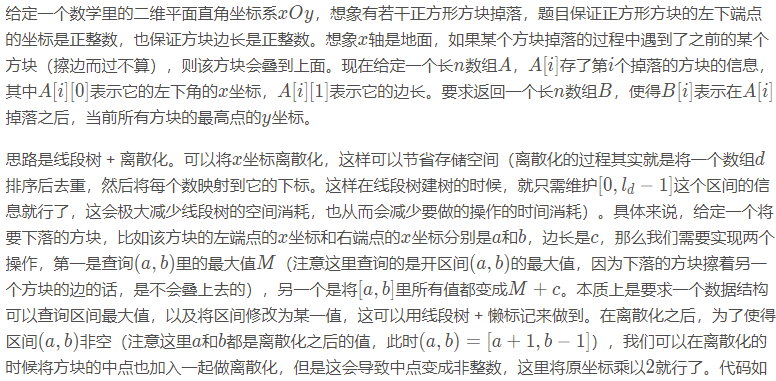
\includegraphics[width=.9\linewidth]{./pic/699.png}

\begin{minted}[fontsize=\scriptsize,linenos=false]{csharp}
public List<Integer> fallingSquares(int[][] a) { // 需要对数据进行离散化处理,离散化的目的是为了线段树处理起来方便;离散的是x轴的横坐标
    List<Integer> x = new ArrayList<>();
    for (int [] v : a) {
        int i = v[0], j = i + v[1];
        x.add(i * 2);
        x.add(j * 2);
        x.add(i + j);
    }
    x = getUniques(x);
    MaxSeg maxSeg = new MaxSeg(x.size());
    List<Integer> ans = new ArrayList<>();
    for (int [] v : a) {
        int i = v[0], j = i + v[1];
        i = getIdxInList(i * 2, x);
        j = getIdxInList(j * 2, x);
        int h = maxSeg.query(1, i+1, j-1);
        maxSeg.update(1, i, j, h + v[1]);
        ans.add(maxSeg.query());
    }
    return ans;
}
int getIdxInList(int v, List<Integer> list) { // 找到 x 在离散化之后的值是多少,其实就是求 xs 里 x 的下标,可以二分来找到
    int l = 0, r = list.size()-1;
    while (l < r) {
        int m = l + (r - l) / 2;
        if (list.get(m) >= v) r = m;
        else l = m + 1;
    }
    return l;
}
List<Integer> getUniques(List<Integer> l) {
    l.sort(Integer::compareTo);
    int j = 0; // 返回结果链表的下标 idx
    for (int i = 0; i < l.size(); i++) {
        if (i == 0 || l.get(j-1) != l.get(i))
            l.set(j++, l.get(i));
    }
    return l.subList(0, j);
}
class MaxSeg {   // 实现一下带懒标记的线段树 : 这棵树好强大
    class Node { // v 是 [l, r] 区间的最大值, lazy 是懒标记
        int l, r, v, lazy;
        public Node(int l, int r) {
            this.l = l;
            this.r = r;
        }
    }
    Node [] tree;
    public MaxSeg(int n) {
        tree = new Node[n << 2]; // n * 2 * 2
        buildTree(1, 0, n-1);    // 下标从 1 开始 自顶向下
    }
    void buildTree(int i, int l, int r) {
        tree[i] = new Node(l, r);
        if (l == r) return;
        int m = l + r >> 1; // (l + r) / 2
        buildTree(i << 1, l, m);
        buildTree(i << 1 | 1, m+1, r);
    }
    void pushUp(int i) { // 自底向上:自左、右叶子节点向顶更新最大值,取左右节点的最大值
        tree[i].v = Math.max(tree[i << 1].v, tree[i << 1 | 1].v);
    }
    void pushDown(int i) { // 懒标记向底、叶子方向推进一层
        int c = tree[i].lazy;
        if (c != 0) { // 打有懒标记
            tree[i].lazy = 0;
            tree[i << 1].v = tree[i << 1 | 1].v = c;
            tree[i << 1].lazy = tree[i << 1 | 1].lazy = c;
        }
    }
    void update(int i, int l, int r, int c) {   // 自顶向下传递懒标记,再自底向上更新父节点的值:取左右子节点的最大值
        if (l <= tree[i].l && tree[i].r <= r) { // 任务不需要下发,可以用懒标记懒住
            tree[i].v = tree[i].lazy = c; // 这里 tree[i].v = tree[i].lazy = c : c 是想要更新到的新值v, 用它来更新懒标记和v值
            return ;
        }
        pushDown(i);  // 任务不得不下发,则先下发给两个孩子
        int m = tree[i].l + tree[i].r >> 1;
        if (l <= m) update(i << 1, l, r, c);  // 回归调用,下传更新至左右子节点
        if (m + 1 <= r) update(i << 1 | 1, l, r, c);
        pushUp(i);  // 孩子完成了任务,再修改自己的值
    }
    int query(int i, int l, int r) {
        if (l <= tree[i].l && r >= tree[i].r) return tree[i].v;
        pushDown(i);
        int ans = 0, m = tree[i].l + tree[i].r >> 1;
        if (l <= m) ans = Math.max(ans, query(i << 1, l, r));
        if (m + 1 <= r) ans = Math.max(ans, query(i << 1 | 1, l, r));
        return ans;
    }
    int query() {
        return tree[1].v;
    }
}
\end{minted}
\item 解题思路与分析: 超简洁版的线段树,效率奇高
\label{sec-3-0-5-3}
\begin{itemize}
\item \url{http://www.noobyard.com/article/p-sxwzvpgp-nz.html}
\item 去找一下原文件中的优化步骤
\begin{minted}[fontsize=\scriptsize,linenos=false]{csharp}
private class Node { // 描述方块以及高度
    int l, r, h, maxR;
    Node left, right;
    public Node(int l, int r, int h, int maxR) {
        this.l = l;
        this.r = r;
        this.h = h;
        this.maxR = maxR;
        this.left = null;
        this.right = null;
    }
}
public List<Integer> fallingSquares(int[][] positions) {
    List<Integer> res = new ArrayList<>(); // 建立返回值
    Node root = null; // 根节点,默认为零
    int maxH = 0; // 目前最高的高度
    for (int[] position : positions) {
        int l = position[0]; // 左横坐标
        int r = position[0] + position[1]; // 右横坐标
        int e = position[1]; // 边长
        int curH = query(root, l, r); // 目前区间的最高的高度
        root = insert(root, l, r, curH + e);
        maxH = Math.max(maxH, curH + e);
        res.add(maxH);
    }
    return res;
}
private Node insert(Node root, int l, int r, int h) {
    if (root == null) return new Node(l, r, h, r);
    if (l <= root.l)
        root.left = insert(root.left, l, r, h);
    else
        root.right = insert(root.right, l, r, h);
    root.maxR = Math.max(r, root.maxR); // 最终目标是仅仅须要根节点更新 maxR
    return root; // 返回根节点
}
private int query(Node root, int l, int r) {
    // 新节点的左边界大于等于目前的maxR的话,直接获得0,不须要遍历了
    if (root == null || l >= root.maxR) return 0; 
    int curH = 0; // 高度
    if (!(r <= root.l || root.r <= l)) // 是否跟这个节点相交
        curH = root.h;
    // 剪枝
    curH = Math.max(curH, query(root.left, l, r));
    if (r > root.l)
        curH = Math.max(curH, query(root.right, l, r));
    return curH;
}
\end{minted}
\end{itemize}
\end{enumerate}
\subsection{1483. Kth Ancestor of a Tree Node - Hard 倍增法 binary lifting}
\label{sec-3-0-6}
You are given a tree with n nodes numbered from 0 to n - 1 in the form of a parent array parent where parent[i] is the parent of ith node. The root of the tree is node 0. Find the kth ancestor of a given node.

The kth ancestor of a tree node is the kth node in the path from that node to the root node.

Implement the TreeAncestor class:

TreeAncestor(int n, int[] parent) Initializes the object with the number of nodes in the tree and the parent array.
int getKthAncestor(int node, int k) return the kth ancestor of the given node node. If there is no such ancestor, return -1.
\begin{enumerate}
\item 解题思路与分析: 倍增 binary lifting
\label{sec-3-0-6-1}

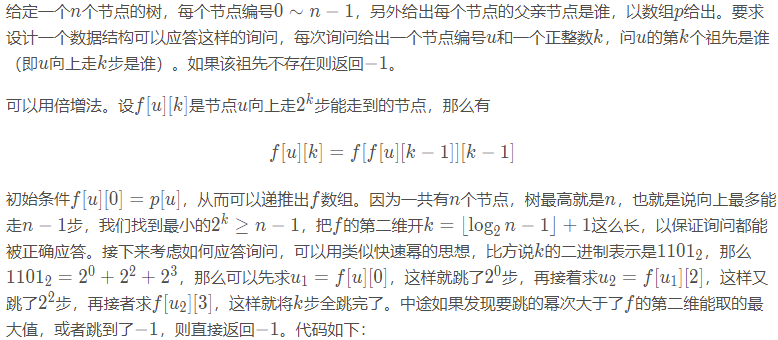
\includegraphics[width=.9\linewidth]{./pic/1483.png}

\begin{itemize}
\item 预处理时间复杂度O(nlogn),每次询问时间O(logn),空间O(nlogn)。

\begin{minted}[fontsize=\scriptsize,linenos=false]{csharp}
    private int [][] p;
    private int log;
    public TreeAncestor(int n, int[] parent) {
        log = (int) (Math.log(n - 1) / Math.log(2)) + 1;
        p = new int[n][log];
        for (int i = 0; i < parent.length; i++) // 初始化p数组
            p[i][0] = parent[i];
        for (int i = 1; i < log; i++) // 按公式递推p数组
            for (int j = 0; j < n; j++) 
                if (p[j][i-1] != -1) 
                    p[j][i] = p[p[j][i-1]][i-1];
                else p[j][i] = -1;
    }
    public int getKthAncestor(int node, int k) {
        int pow = 0;
        while (k > 0) {
            if (pow >= log || node == -1) return -1;
            if ((k & 1) == 1) 
                node = p[node][pow];
            k >>= 1;
            pow++;
        }
        return node;
    }
\end{minted}
\end{itemize}
\item 解题思路与分析
\label{sec-3-0-6-2}
\begin{minted}[fontsize=\scriptsize,linenos=false]{csharp}
    Map<Integer, List<Integer>> adj;
    int [][] par;
    public TreeAncestor(int n, int[] parent) {
        par = new int [n][30]; // 30 , 16: 不能证它是一棵很平衡的二叉树
        adj = new HashMap<>();
        for (int i = 0; i < n; i++) {
            Arrays.fill(par[i], -1);
            adj.put(i, new ArrayList<>());
        }
        for (int i = 0; i < parent.length; i++) 
            if (parent[i] != -1) {
                adj.get(parent[i]).add(i); // 自顶向下: 父 --》子节点
                par[i][0] = parent[i];     // 每个子节点的第一个父节点(2^0 = 1),即为父节点 // 自底向上: 子节点: 2^0父节点、 2^1节点、 2^2节点
            }
        dfs(0);
    }
    public int getKthAncestor(int node, int k) {
        for (int i = 0; k > 0; i++, k >>= 1) // k /= 2
            if ((k & 1) == 1) {
                node = par[node][i];
                if (node < 0) return -1;
            }
        return node;
    }
    private void dfs(int idx) { // 自顶向下:从父节点遍历子节点
        for (int i = 1; par[idx][i-1] >= 0; i++) // 穷追塑源:一直找到整棵树的根节点: 0
            par[idx][i] = par[par[idx][i-1]][i-1]; // 这里多想想
        for (int next : adj.get(idx)) 
            dfs(next);
    }
\end{minted}
\end{enumerate}
\subsection{236 二叉树的最近公共祖先}
\label{sec-3-0-7}

\subsection{1505. Minimum Possible Integer After at Most K Adjacent Swaps On Digits - Hard BIT树状数组}
\label{sec-3-0-8}
You are given a string num representing the digits of a very large integer and an integer k. You are allowed to swap any two adjacent digits of the integer at most k times.

Return the minimum integer you can obtain also as a string.
\begin{enumerate}
\item 解题思路与分析
\label{sec-3-0-8-1}
\begin{minted}[fontsize=\scriptsize,linenos=false]{csharp}
public String minInteger(String t, int k) {
    int n = t.length();
    t = " " + t;
    char [] s = t.toCharArray();
    ArrayDeque<Integer> [] q = new ArrayDeque [10];
    for (int i = 1; i <= n; i++) {
        int j = s[i] - '0';
        if (q[j] == null) q[j] = new ArrayDeque<>();
        q[j].offerLast(i);
    }
    BIT bit = new BIT(n);
    StringBuilder sb = new StringBuilder();
    for (int i = 1; i <= n; i++) {
        for (int j = 0; j < 10; j++) { // 从小数值往大数值遍历
            if (q[j] == null || q[j].isEmpty()) continue;
            int top = q[j].peekFirst(), pos = top + bit.sum(top); // pos是最优解的位置,最优解的位置是原来的位置加上偏移量
            if (pos - i <= k) {
                k -= pos - i;
                sb.append(j);
                q[j].pollFirst();
                bit.add(1, 1); // 更新[1, t)这段的值每个加1,即向右偏移1位.为什么要 从1开始更新:假装每次都移动到最前端,方便计算 ?
                bit.add(top, -1);
                break;
            }
        }
    }
    return sb.toString();
}
class BIT { // 开一个树状数组类,维护每个位置的字符的向右的偏移量 ? 向左偏移量
    private int n;
    private int [] a;
    public BIT(int n) {
        this.n = n;
        this.a = new int [n+1];
    }
    public void add(int idx, int v) { // 只有发生偏移,才移动某段区间的值
        while (idx <= n) {
            a[idx] += v;
            idx += lowbit(idx);
        }
    }
    public int sum(int idx) { // 得到以 i 为下标1-based的所有子、叶子节点的和, 也就是[1, idx]的和,1-based
        int ans = 0;
        while (idx > 0) {
            ans += a[idx];
            idx -= lowbit(idx);
        }
        return ans;
    }
    int lowbit(int x) {
        return x & -x;
    }
}
\end{minted}
\end{enumerate}
\chapter{Trie}
\label{sec-4}
应用
Trie树最直观的定义就是LinkedList of HashMap。所以Trie和HashMap都可以用来查询某个单词是否在字典当中。我们需要知道他们的优缺点。
优点:
支持字符级别的查询,比如说我们需要在matrix当中通过traverse构造单词,那么这个单词是一个一个字符形成的,我们可以在traverse的每一步去检验当前路径是否可以形成valid word。另外,对于含有regex符号的字符串,我们需要一个字符一个字符的考虑,这种情况下我们也需要通过trie去查找。
节省空间,相同的prefix只存一遍,而HashMap需要存很多遍。
缺点:实现起来较麻烦,大部分题目使用Trie都是overkill,所以除非需要支持字符级别的查询,否则HashMap更好。
操作: 三个操作:
insert
search
startWith
其中insert记得把最后一个node标记为isEnd = true。其中search和startWith都可以通过同一个searchHelper helper method来实现,我们只需要return 最后一个node就可以,如果isEnd == true,那么说明找到一个完整的单词,否则至少找到了prefix。别忘了使用trie的第一步是preprocess,把字典里的所有word加入到trie树当中。
题目
\section{208. Implement Trie (Prefix Tree)}
\label{sec-4-1}
\subsection{212. Word Search II}
\label{sec-4-1-1}
\subsection{211. Add and Search Word - Data structure design (Facebook店面)}
\label{sec-4-1-2}
\subsection{14. Longest Common Prefix (这道题可以稍作改编,比如说string list会经常update,会经常query,那这时很明显用trie更好)}
\label{sec-4-1-3}
\subsection{440. K-th Smallest in Lexicographical Order -  Hard}
\label{sec-4-1-4}
Given two integers n and k, return the kth lexicographically smallest integer in the range [1, n].
\begin{enumerate}
\item 解题思路与分析
\label{sec-4-1-4-1}
就像dfs时当我们需要两个字符串,遍历字符串,我们并不需要看的去遍历字符串,我们只要移动下标就可以了

这里我们并不需要真的去建和遍历这样一个字典,我们只要理清数字个数之间的关系就可以了

还要一个典型案例,把它找出来。。。。 todo

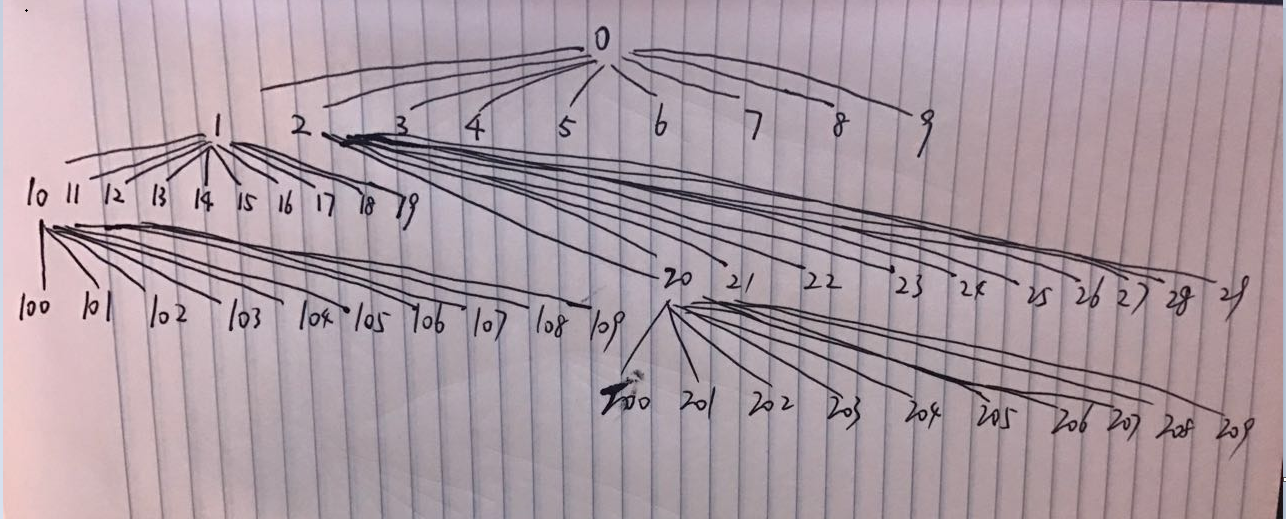
\includegraphics[width=.9\linewidth]{./pic/trie.png}

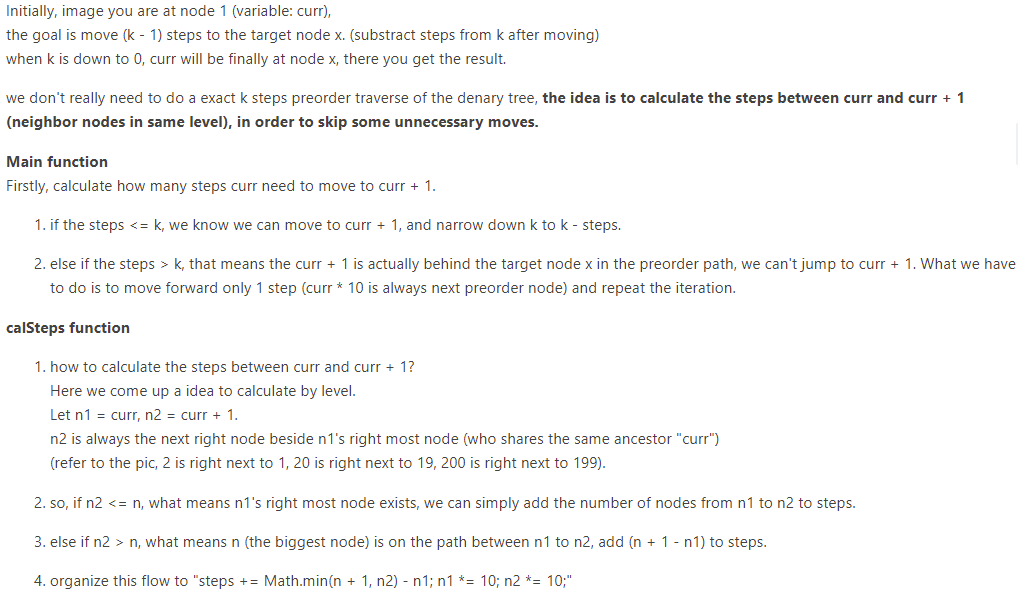
\includegraphics[width=.9\linewidth]{./pic/trie2.png}

\begin{minted}[fontsize=\scriptsize,linenos=false]{csharp}
private int calSteps(int n, long n1, long n2) { // n1 和 n2得是long类型的, int会产生溢出, 不能通过这个案例: 输入n=681692778, k=351251360, 预期结果=416126219
    int steps = 0;
    while (n1 <= n) {
        steps += Math.min(n2, n+1) - n1;
        n1 *= 10;
        n2 *= 10;
    }
    return steps;
}
public int findKthNumber(int n, int k) {
    int cur = 1; //根据题意, 第一个数是1
    --k;         //第一个是1, 所以再找出k-1个数后就知道第k个数是多少了
    while (k > 0) {
        int steps = calSteps(n, cur, cur+1);
        if (steps <= k) { //横向扩展, 相当于+steps,
            cur += 1;
            k -= steps;
        } else {          //steps > k; 纵向扩展, 相当于+1
            cur *= 10;
            k -= 1;
        }
    }
    return cur;
}
\end{minted}
\end{enumerate}

\subsection{421. Maximum XOR of Two Numbers in an Array}
\label{sec-4-1-5}
Given an integer array nums, return the maximum result of nums[i] XOR nums[j], where 0 <= i <= j < n.

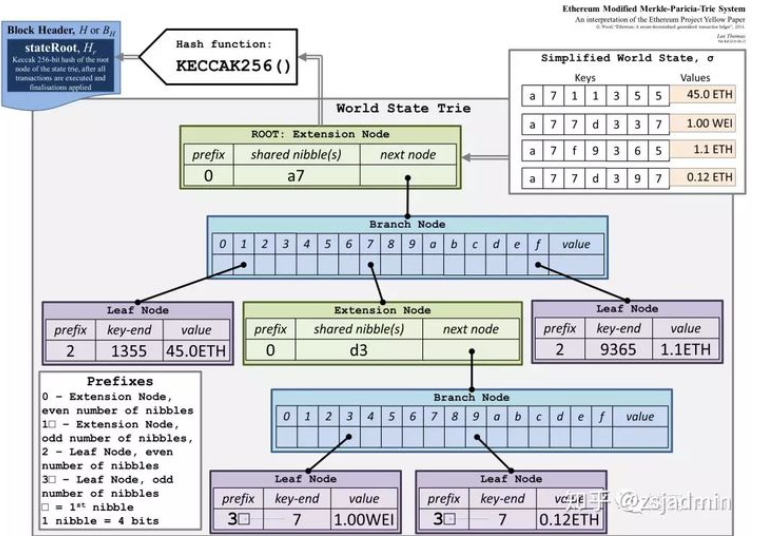
\includegraphics[width=.9\linewidth]{./pic/numTrie.png}

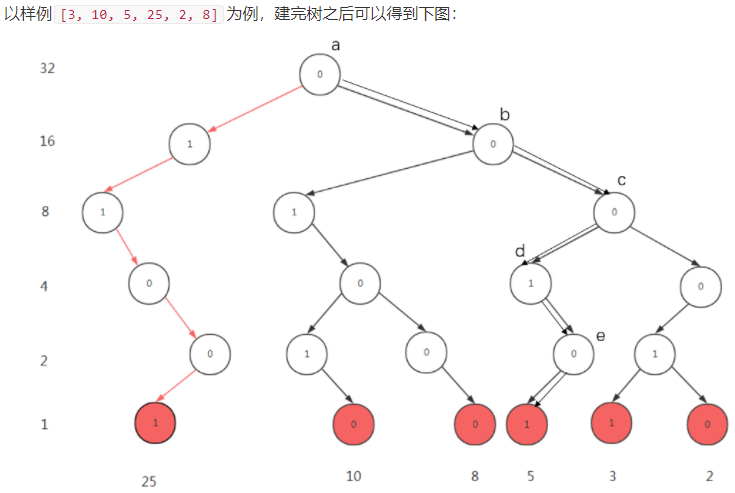
\includegraphics[width=.9\linewidth]{./pic/numTrie2.png}

左儿子为1的分支,右儿子为0的分支。

然后依次枚举每个数,在Trie树中找到与它异或结果最大的数。

这一步可以贪心来做:

从高位到低位,依次在Trie树中遍历,每次尽量走到与当前位不同的分支,这样可以使得找到的数与当前数在当前二进制位的异或结果是1,从而可以得到尽量大的结果。

如上图所示,我们用25来举例说明,它的二进制表示是(11001):

\begin{minted}[fontsize=\scriptsize,linenos=false]{csharp}
最初指针在根节点(编号是a的点),我们从25的二进制表示的最高位开始枚举;
  由于最高位是1,我们走到0分支,走到b点;
  次高位是1,我们继续往右儿子走,走到c点;
  下一位是0,我们往左走,走到d点;
  下一位是0,我们希望往左走,但发现左儿子不存在,所以只能往右走,走到e点;
  最后一位是1,我们希望往右走,但发现右儿子不存在,所以只能往左走,最终走到5;
所以和25异或值最大的数是5, 25 ^ 5 = 28。
\end{minted}
\begin{minted}[fontsize=\scriptsize,linenos=false]{csharp}
public class Trie {
    private class Node { // 这我自己写的乱代码,贴在这里很不相关,也需要先测试一下
        public int val;
        public boolean isExist;
        public Node [] next;
        public Node(boolean isExist) {
            this.isExist = isExist;
            next = new Node[2];
            val = 0;
        }
        public Node() { this(false); }
        public Node(int va) {
            this(true);
            this.val = va;
        }
    }
    private Node root;
    public Trie() { root = new Node(); }
    public void insert(int va) {
        Node cur = root;
        for (int i = 31; i >= 0; i--) {
            int tmp = (va >> i) & 1;
            if (cur.next[tmp] == null)
                cur.next[tmp] = new Node();
            cur = cur.next[tmp];
        }
        cur.isExist = true;
    }
    public int search(int va) {
        int max = 0;
        Node cur = root;
        for (int i = 31; i >= 0; i--) {
            int t = (va >> i) & 1;
            if (cur.next[t^1] != null) {
                max += (1 << i);
                cur = cur.next[t^1];
            } else cur = cur.next[t&1];
        }
        return max;
    }
}
\end{minted}

\begin{enumerate}
\item 另一种位操作法
\label{sec-4-1-5-1}

\begin{itemize}
\item 学到了异或操作的一个重要性质:a\^{}b = c, 则有 a\^{}c = b,且 b\^{}c = a;
\end{itemize}

我们还需要用上一个异或的特性,假设a和b产生了最终的答案max,即a \^{} b = x,那么根据异或的特性,a \^{} x = b。同理,a和b的最高位(前n位)也有相同的性质。

先以最高位为例子,我们可以把所有的数字的最高位放到一个HashSet里面,然后使用1与set里面的所有数字进行异或,如果得出的结果仍然在set里面,那么最终结果的最高位必然为1,否则为0。也即,先假定结果为1,然后与set中所有数字异或,假定a与1异或得到结果b(a \^{} 1 = b),而b仍然在set里面,那么说明set中有两个数字异或能得到1(a \^{} b = 1)。否则,set中没有两个数字能够异或得到1,那么最终结果的最高位为1的假设失败,说明最终结果的最高位为0。以此类推可以得到第二位、第三位。。。的数字。

再做一下推广,我们将所有数字的前N位放到一个HashSet里面,然后使用之前N-1位得到的最大值前缀prefix与set里面的所有数字进行异或,如果得出的结果仍然在set中,那么第N位必然为1,否则为0。

举个例子,给定数组[14, 11, 7, 2],二进制表示分别为[1110, 1011, 0111, 0010]。题目说了,数字最长不会超过32位,所以应从i = 31开始,但是所有数字中最多位4位数,简单起见,我直接从最高位i=3开始
\begin{minted}[fontsize=\scriptsize,linenos=false]{csharp}
[14,   11,   7,    2]
[1110, 1011, 0111, 0010]
1. i = 3, set = {1000, 0000} => max = 1000
2. i = 2, set = {1100, 1000, 0100, 0000} => max = 1100
3. i = 1, set = {1110, 1010, 0110, 0010} => max = 1100
4. i = 0, set = {1110, 1011, 0111, 0010} => max = 1100
\end{minted}
\begin{minted}[fontsize=\scriptsize,linenos=false]{csharp}
public int findMaximumXOR(int[] nums) { // 这种解法没有用到上面的这个trie呀
    int n = nums.length;
    int mask = 0, max = 0;
    HashSet<Integer> s = new HashSet<>();
    for (int i = 31; i >= 0; --i) { // i == 31时
        mask = mask | 1 << i;     // 为获取前n位的临时变量     
        for (int va : nums) 
            s.add(va & mask);     // 将所有数字的前n位放入set中
        int tmp = max | (1 << i); // 假定第n位为1,前n-1位max为之前迭代求得
        for (Integer va : s) 
            if (s.contains(va ^ tmp)) { // 查看`b`是否在 // i == 31, (va^tmp):  -2147483648
                max = tmp;              // b存在,第n位为1
                break;
            }
        s.clear();
    }
    return max;
}
// 此解法时间复杂度为O(32n)=O(n),空间复杂度上,我们使用了一个HashSet用于存储所有数字,因此空间复杂度是O(n)
\end{minted}
\end{enumerate}

\subsection{1617. Count Subtrees With Max Distance Between Cities - Hard}
\label{sec-4-1-6}
There are n cities numbered from 1 to n. You are given an array edges of size n-1, where edges[i] = [ui, vi] represents a bidirectional edge between cities ui and vi. There exists a unique path between each pair of cities. In other words, the cities form a tree.

A subtree is a subset of cities where every city is reachable from every other city in the subset, where the path between each pair passes through only the cities from the subset. Two subtrees are different if there is a city in one subtree that is not present in the other.

For each d from 1 to n-1, find the number of subtrees in which the maximum distance between any two cities in the subtree is equal to d.

Return an array of size n-1 where the dth element (1-indexed) is the number of subtrees in which the maximum distance between any two cities is equal to d.

Notice that the distance between the two cities is the number of edges in the path between them.
\begin{itemize}
\item So apparently the brute-force approach passed this question. I guess for future contests, I should really pay attention to the input size\ldots{}
\end{itemize}
\begin{enumerate}
\item 解题思路与分析:
\label{sec-4-1-6-1}

自己凭感觉写的,看别人的代码(尤其写得比较烦琐的前提下)不如自己的代码简炼

\begin{minted}[fontsize=\scriptsize,linenos=false]{csharp}
public int[] countSubgraphsForEachDiameter(int n, int[][] edges) { 
    int m = n-1, range = 1 << m, root = 0, cnt = 0;
    int [] ans = new int [m];
    for (int i = 1; i < range; i++) {
        root = -1;
        Map<Integer, List<Integer>> adj = new HashMap<>();
        for (int j = 0; j < m; j++)  // m edges
            if (((i >> j) & 1) == 1) {
                int [] e = edges[j];
                if (root == -1) root = e[0];
                adj.computeIfAbsent(e[0], z -> new ArrayList<>()).add(e[1]);
                adj.computeIfAbsent(e[1], z -> new ArrayList<>()).add(e[0]);
            }
        cnt = Integer.bitCount(i);
        Set<Integer> vis = new HashSet<>();
        max = 1;
        dfs(root, -1, adj, vis);
        if (vis.size() != cnt + 1) continue;
        ans[max-1]++;
    }
    return ans;
}
int max = 1;
private int dfs(int u, int p, Map<Integer, List<Integer>> m, Set<Integer> vis) { // 树的最大直径:
    vis.add(u);
    if (m.get(u).size() == 1 && m.get(u).get(0) == p) return 1; // 叶子节点 
    int fst = 0, sec = 0;
    for (Integer v : m.get(u)) {
        if (v == p) continue;
        int cur = dfs(v, u, m, vis);
        if (cur >= fst) {
            sec = fst;
            fst = cur;
        } else sec = Math.max(sec, cur);
    }
    max = Math.max(max, fst + sec); // bug: 这里 fst + sec 不需要 +1
    return fst + 1;
}
\end{minted}
\begin{itemize}
\item 另一种位操作法
\end{itemize}
\begin{minted}[fontsize=\scriptsize,linenos=false]{csharp}
One way in which we can find the diameter of a tree is using DFS, just like if our tree is represented using tree nodes instead of as grpah
    1. Make a call to DFS from any node as root, lets say 1 as root
    2. Maintain a global max parameter
    3. For each call to dfs, of all current nodes children (excluding parent)
       find top two distances from current node to any leaf reachable from current node
    4. Sum of these top two distances froms the longes path passing through current node to all its children. Update if this path is maximum
    5. return 1 + top distance for this dfs call. Need to add 1 since,
       max length of path that can be reached from current ndoe is current ndoe + max distance reachable from current ndoes's children
\end{minted}
\begin{minted}[fontsize=\scriptsize,linenos=false]{csharp}
public int [] countSubgraphsForEachDiameter(int n, int[][] edges) {
    ans = new int [n-1];
    for (int [] i : edges) { // if our node is 5, we store it as 1 << 4 which is 2^4
        graph.computeIfAbsent(1 << (i[0]-1), ArrayList::new).add(1 << (i[1]-1));
        graph.computeIfAbsent(1 << (i[1]-1), ArrayList::new).add(1 << (i[0]-1));
    }
    int range = (1 << n) - 1;  // (int)Math.pow(2, n) - 1;
    for (int subset = 3; subset <= range; subset++) {
        boolean isPowerOf2 = subset != 0 && (subset & (subset - 1)) == 0; // is power of 2
        if (isPowerOf2) continue;      // Single node subtrees can be excluded.
        max = 0; vis = 0;
        dfs(subset, Integer.highestOneBit(subset), -1); // Integer.highestOneBit(subset): subset: 0b1100, highest: 0b1000
        if (vis == subset)   // If visited is not equal to our current subset, all nodes are not reachable.
            ans[max - 1] ++; // In otherwords is not a proper subtree, hence dont include in the maxwer
    }
    return ans;
}
Map<Integer, List<Integer>> graph = new HashMap<>();
int max = 0, vis = 0;
int [] ans;
private int dfs(int subset, int cur, int pre) {
    if ((subset & cur) == 0) return 0; // 只遍历子集中存在的节点,换句话说,只遍历子集中存在的边,这样总图只建一遍就可以了
    vis = vis | cur; 
    int fstMax = 0, sndMax = 0;
    for (Integer next : graph.get(cur)) {
        if (next == pre) continue;
        int dist = dfs(subset, next, cur);
        if (dist > fstMax) {
            sndMax = fstMax;
            fstMax = dist;
        } else sndMax = Math.max(sndMax, dist);
    }
    max = Math.max(max, fstMax + sndMax); // top two distances from this node c
// top distance this cur node to any leaf is topdistance from c's children + 1. Adding 1 since we need to include cur node
    return 1 + fstMax;
}
\end{minted}
\begin{itemize}
\item 以前参考过的代码
\end{itemize}
\begin{minted}[fontsize=\scriptsize,linenos=false]{csharp}
public int [] countSubgraphsForEachDiameter(int n, int[][] edges) {
    int [] res = new int [n-1];
    List<List<int []>> subsets = new ArrayList<>();
    generateSubsets(edges, new ArrayList<int []>(), subsets, 0);
    for (List<int []> subset : subsets) 
        solve(subset, res);
    return res;
}
private void solve(List<int []> subset, int [] res) {
    if (!isValidGraph(subset)) return;
    Map<Integer, List<Integer>> graph = new HashMap<>();
    for (int [] eg : subset) {
        graph.computeIfAbsent(eg[0], k -> new ArrayList<>()).add(eg[1]);
        graph.computeIfAbsent(eg[1], k -> new ArrayList<>()).add(eg[0]);
    }
    int max = 1;
    for (Integer key : graph.keySet()) {
        if (graph.get(key).size() == 1) {
            int [] longest = new int [] {1}; // 减少global变量的数量
            Set<Integer> vis = new HashSet<>();
            vis.add(key);
            dfs(graph, vis, key, longest, 0);
            max = Math.max(max, longest[0]);
        }
    }
    res[max - 1]++;
}
private void dfs(Map<Integer, List<Integer>> graph, Set<Integer> vis, int idx, int [] longest, int level) {
    longest[0] = Math.max(longest[0], level);
    for (Integer node : graph.get(idx)) 
        if (vis.add(node)) // Set.add(element) return false if it contains element already
            dfs(graph, vis, node, longest, level + 1);
}
private boolean isValidGraph(List<int []> subset) {
    Set<Integer> nodes = new HashSet<>();
    for (int [] cur : subset) {
        nodes.add(cur[0]);
        nodes.add(cur[1]);
    }
    return nodes.size() - 1 <= subset.size();
}
private void generateSubsets(int [][] arr, List<int []> cur, List<List<int []>> res, int idx) {
    if (idx == arr.length) return; // arr.length <= 15, 用回塑法直接生成subsets,但是这是相对耗时的操作
    for (int i = idx; i < arr.length; i++) {
        cur.add(arr[i]);
        res.add(new ArrayList<>(cur));
        generateSubsets(arr, cur, res, i+1);
        cur.remove(cur.size()-1);
    }
}
\end{minted}
\end{enumerate}

\subsection{1938. Maximum Genetic Difference Query - Hard 离线算法、离线思维、批量处理、顺序无关}
\label{sec-4-1-7}
There is a rooted tree consisting of n nodes numbered 0 to n - 1. Each node's number denotes its unique genetic value (i.e. the genetic value of node x is x). The genetic difference between two genetic values is defined as the bitwise-XOR of their values. You are given the integer array parents, where parents[i] is the parent for node i. If node x is the root of the tree, then parents[x] == -1.

You are also given the array queries where queries[i] = [nodei, vali]. For each query i, find the maximum genetic difference between vali and pi, where pi is the genetic value of any node that is on the path between nodei and the root (including nodei and the root). More formally, you want to maximize vali XOR pi.

Return an array ans where ans[i] is the answer to the ith query.
\begin{minted}[fontsize=\scriptsize,linenos=false]{csharp}
// 可以从根节点开始,对整棵树进行一次深度优先遍历,即:
// 当我们第一次遍历到某一节点 ii 时,我们将 ii 放入「数据结构」中;
// 当我们遍历完所有节点 ii 的子节点,即将回溯到 ii 的父节点前,我们将 ii 从「数据结构」中移除。
// 这样一来,我们就可以通过「离线」的思想将每一个询问在遍历到节点 val}_ival 时进行求解。这是因为,如果当前正在遍历节点 val}_ival
// 那么数据结构中就存放着所有从根节点到节点 val}_ival 的路径上的所有节点。
// 此时,我们只需要找出数据结构中使得 p_i \oplus val}_ip 达到最大值的节点 p_ip 即可。
// 而深度优先搜索过程中,当前入队的部分正是该节点及其所有层级的父节点,因此可结合 DFS 方法进行离线搜索。
// 对最大异或值的计算,可结合字典树方法进行。
// 本题需涉及对字典树中数值的删除操作,为简化代码,可在字典树的节点中设计一个计数器,记录当前该节点对应的数字个数,从而避免删除实际节点。
public class Trie {
    static final int H = 18; // 树高度,本题val<=2*10^5<2^18
    Trie [] next;
    int cnt;                 // 当前节点对应的数值个数,简化删除操作
    public Trie() {
        this.next = new Trie[2];
        this.cnt = 0;
    }
    public void insert(int va) { // 插入数值
        Trie r = this;
        for (int i = H-1; i >= 0; i--) {
            int bit = (va >> i) & 1;
            if (r.next[bit] == null) 
                r.next[bit] = new Trie();
            r = r.next[bit];
            r.cnt++;
        }
    }
    private void removeVal(int v) { // 删除数值
        Trie r = this;
        for (int i = H-1; i >= 0; i--) {
            int bit = (v >> i) & 1;
            r = r.next[bit];
            r.cnt--;
        }
    }
    public int search(int va) { // 针对数值查询当前字典树对应的最大异或值
        Trie r = this;
        int max = 0;
        for (int i = H-1; i >= 0; i--) {
            int bit = (va >> i) & 1 ^ 1;
            if (r == null) return -1;
            if (r.next[bit] != null && r.next[bit].cnt > 0) {
                max += (1 << i);
                r = r.next[bit];
            } else
                r = r.next[bit ^ 1];
        }
        return max;
    }
}
private void dfs(int idx) { // 深度优先搜索
    trie.insert(idx);       // 当前节点加入字典树
    if (queVal.containsKey(idx)) // 处理针对当前节点的查询
        for (int i = 0; i < queVal.get(idx).size(); i++) 
            ans[queId.get(idx).get(i)] = trie.search(queVal.get(idx).get(i));
    if (tree.containsKey(idx))   // 当前节点存在子节点
        for (int n : tree.get(idx)) 
            dfs(n);
    trie.removeVal(idx);         // 从字典树中删除当前节点
}
Map<Integer, List<Integer>> tree;  // 树中各个节点对应的子节点
Map<Integer, List<Integer>> queVal;// 树中各个节点对应的查询值
Map<Integer, List<Integer>> queId; // 树中各个节点对应的queries下标
Trie trie;                         // 字典树根节点
int [] ans;
public int[] maxGeneticDifference(int[] parents, int[][] queries) {
    int n = parents.length, m = queries.length, root = -1;
    this.tree = new HashMap<>();
    for (int i = 0; i < n; i++) { // 记录树中各个节点对应的子节点
        if (parents[i] != -1) {   // Note: 当作有向树图来处理 !!!
            tree.computeIfAbsent(parents[i], k -> new ArrayList<>());
            tree.get(parents[i]).add(i);
        } else root = i;  
    }
    this.queVal = new HashMap<>();
    this.queId = new HashMap<>();
    for (int i = 0; i < m; i++) {
        int nid = queries[i][0], val = queries[i][1];
        queVal.computeIfAbsent(nid, k -> new ArrayList<>()).add(val);
        queId.computeIfAbsent(nid, k -> new ArrayList<>()).add(i);
    }
    this.ans = new int [m];
    this.trie = new Trie();
    dfs(root);
    return ans;
}
\end{minted}

复杂度分析

时间复杂度:O((n+q) $\log$ C)O((n+q)logC),其中 qq 是数组 queries\}queries 的长度,$\log$ C = 18logC=18 是本题中最大的数的二进制表示的位数。在深度优先遍历的过程中,访问的节点个数为 nn,每个节点需要 O($\log$ C)O(logC) 的时间在一开将其加入字典树以及回溯前将其从字典树中移除。对于数组 queries\}queries 中的每一个询问,我们需要 O($\log$ C)O(logC) 的时间得到答案。因此总时间复杂度为 O((n+q) $\log$ C)O((n+q)logC)。

空间复杂度:O(n$\log$ C + q)O(nlogC+q)。我们需要 O(n)O(n) 的空间存储树本身,O(n $\log$ C)O(nlogC) 的空间存储字典树,O(q)O(q) 的空间存储将询问进行离线,分配到每个节点上。

\subsection{792. Number of Matching Subsequences - Medium}
\label{sec-4-1-8}
Given a string s and an array of strings words, return the number of words[i] that is a subsequence of s.

A subsequence of a string is a new string generated from the original string with some characters (can be none) deleted without changing the relative order of the remaining characters.

For example, "ace" is a subsequence of "abcde".
\begin{minted}[fontsize=\scriptsize,linenos=false]{csharp}
// 我们需要使用每个字典中的单词去和S比较,看它是否是S的子序列。不过这种比较非常耗费时间,因此我们需要对S进行一下预处理。
// 首先定义一个二维数组arr[][],其中 arr[i][j]代表距离S中第i位字符最近的j字符的位置。
// 换句话说,我们需要遍历一边字符串,记录下字符串S每一位上的字符,在它右侧距离它最近的a-z分别在哪。
public int numMatchingSubseq(String s, String[] words) {
    int n = s.length();
    int [][] arr = new int [n][26]; // 预处理用的数组
    for (int i = n-2; i >= 0; i--) {// 预处理
        arr[i] = Arrays.copyOf(arr[i+1], 26);
        arr[i][s.charAt(i+1)-'a'] = i+1;
    }
    int res = 0, idxAtS = 0, idx = 0, cur = 0;
    for (String v : words) {        // 比较每一个单词
        idxAtS = 0;                 // 对应S的下标
        idx = 0;                    // 当前单词下标
        if (v.charAt(0) == s.charAt(0)) { // 如果当前单词首字符等于S首字符
            idx ++;                 // 当前单词下标加一
            if (v.length() == 1) res++;      // 如果当前单词长度只有1,说明当前单词已经遍历结束,结果加一
        }
        while (idx < v.length()) {            // 继续比较单词接下来的字符,在S中是否存在
            cur = v.charAt(idx) - 'a';
            if (arr[idxAtS][cur] == 0) break; // 如果indexAtS之后不存在c,当前单词不合法
            idxAtS = arr[idxAtS][cur]; // 将indexAtS更新为c在S中的位置
            if (++idx == v.length()) res++;     // index加一, 如果index为单词最后一位,代表单词中所有字符均在S中找到
        }
    }
    return res;
}
\end{minted}

\subsection{472. Concatenated Words - Hard}
\label{sec-4-1-9}
Given an array of strings words (without duplicates), return all the concatenated words in the given list of words.

A concatenated word is defined as a string that is comprised entirely of at least two shorter words in the given array.

Example 1:
\begin{minted}[fontsize=\scriptsize,linenos=false]{csharp}
Input: words = ["cat","cats","catsdogcats","dog","dogcatsdog","hippopotamuses","rat","ratcatdogcat"]
Output: ["catsdogcats","dogcatsdog","ratcatdogcat"]
Explanation: "catsdogcats" can be concatenated by "cats", "dog" and "cats"; 
"dogcatsdog" can be concatenated by "dog", "cats" and "dog"; 
"ratcatdogcat" can be concatenated by "rat", "cat", "dog" and "cat".
\end{minted}
\begin{itemize}
\item 切记: dfs 深搜 + 记忆
\end{itemize}
\begin{minted}[fontsize=\scriptsize,linenos=false]{csharp}
// 切记: dfs 深搜 + 记忆 // Trie with memo, Time: o(m*2^n)
public class Trie { 
    boolean isWord;
    Trie [] children;
    public Trie() {
        isWord = false;
        children = new Trie[26];
    }
}
public void insert(String word) { 
    Trie cur = root;
    for (int i = 0; i < word.length(); i++) {
        char c = word.charAt(i);
        if (cur.children[c-'a'] == null)
            cur.children[c-'a'] = new Trie();
        cur = cur.children[c-'a'];
    }
    cur.isWord = true;
}     
public boolean isConcatenated(String word, int idx, int cnt, HashMap<Integer, Boolean> memo) {
    if (memo.containsKey(idx)) return memo.get(idx);
    if (idx == word.length()) {
        memo.put(idx, cnt > 1);
        return cnt > 1;
    }
    Trie cur = root;
    for (int i = idx; i < word.length(); i++) {
        char c = word.charAt(i);
        if (cur.children[c-'a'] == null) {
            memo.put(idx, false);
            return false;
        } else {
            cur = cur.children[c-'a'];
            if (cur.isWord && isConcatenated(word, i+1, cnt+1, memo)) {
                memo.put(idx, true);
                return true;
            }
        }
    }
    memo.put(idx, false);
    return false;
}
Trie root = new Trie();
public List<String> findAllConcatenatedWordsInADict(String[] words) {
    for (String word : words) 
        insert(word);
    List<String> res = new ArrayList<>();
    for (String word : words) 
        if (isConcatenated(word, 0, 0, new HashMap<Integer, Boolean>()))
            res.add(word);
    return res;
}
\end{minted}
\begin{itemize}
\item 一种稍微优化了一下的方法,逻辑就相对复杂一点儿,参考一下
\end{itemize}
\begin{minted}[fontsize=\scriptsize,linenos=false]{csharp}
public class Trie { // Trie with memo, Time: o(m*2^n)
    boolean isKey;
    Trie [] child;
    public Trie() {
        this.isKey = false;
        child = new Trie[26];
    }
    public void insert(String s) {
        int [] memo = new int [s.length()];
        Trie p = this;
        char [] sArr = s.toCharArray();
        boolean added = false;
        for (int i = 0; i < sArr.length; i++) {
            char c = sArr[i];
            if (p.child[c-'a'] == null)
                p.child[c-'a'] = new Trie();
            p = p.child[c-'a'];
            if (p.isKey && isConcatenated(s, i+1, 0, memo) && !added) {
                res.add(s);
                added = true;
            }
        }
        p.isKey = true;
    }     // 这么看来,我还没能透彻理解dfs深搜中的重复,什么时候应该拥有记忆?!!!
    public boolean isConcatenated(String s, int start, int cnt, int [] memo) {
        if (start == s.length() && cnt > 0) return true; 
        if (memo[start] != 0) return memo[start] == 1;
        Trie p = this;
        char [] sArr = s.toCharArray();
        for (int i = start; i < sArr.length; i++) {
            char c = sArr[i];
            Trie cur = p.child[c-'a'];
            if (cur == null) {
                memo[start] = -1;
                return false;
            } else {
                if (cur.isKey && isConcatenated(s, i+1, cnt+1, memo)) {
                    memo[start] = 1;
                    return true;
                }
                p = cur;
            }
        }
        memo[start] = -1;
        return false;
    }
}
// Sort the words based on length
// Use trie to store words: while adding, checking if it is concatenated
// While checking, use dfs + memo
List<String> res = new ArrayList<>();
public List<String> findAllConcatenatedWordsInADict(String[] words) {
    Arrays.sort(words, (x, y) -> Integer.compare(x.length(), y.length()));
    Trie tree = new Trie();
    for (String word : words) 
        tree.insert(word);
    return res;
}
\end{minted}

\subsection{1948. Delete Duplicate Folders in System - Hard}
\label{sec-4-1-10}
Due to a bug, there are many duplicate folders in a file system. You are given a 2D array paths, where paths[i] is an array representing an absolute path to the ith folder in the file system.

For example, ["one", "two", "three"] represents the path "/one/two/three".
Two folders (not necessarily on the same level) are identical if they contain the same non-empty set of identical subfolders and underlying subfolder structure. The folders do not need to be at the root level to be identical. If two or more folders are identical, then mark the folders as well as all their subfolders.

For example, folders "/a" and "/b" in the file structure below are identical. They (as well as their subfolders) should all be marked:
\begin{minted}[fontsize=\scriptsize,linenos=false]{csharp}
/a
/a/x
/a/x/y
/a/z
/b
/b/x
/b/x/y
/b/z
\end{minted}
However, if the file structure also included the path "/b/w", then the folders "/a" and "/b" would not be identical. Note that "/a/x" and "/b/x" would still be considered identical even with the added folder.

Once all the identical folders and their subfolders have been marked, the file system will delete all of them. The file system only runs the deletion once, so any folders that become identical after the initial deletion are not deleted.

Return the 2D array ans containing the paths of the remaining folders after deleting all the marked folders. The paths may be returned in any order.
\begin{minted}[fontsize=\scriptsize,linenos=false]{csharp}
public class Node {
    String name;
    Map<String, Node> children = new HashMap<>();
    private String hashCode = null;
    public Node (String name) {
        this.name = name;
    }
    public void add(List<String> path) {
        Node cur = this;
        for (String file : path) {
            if (!cur.children.containsKey(file))
                cur.children.put(file, new Node(file));
            cur = cur.children.get(file);
        }
    }
    public String getHashCode() {
        if (hashCode == null)
            hashCode = compueteHash();
        return hashCode;
    }
    private String compueteHash() {
        StringBuilder sb = new StringBuilder();
        List<Node> nodes = new ArrayList<>();
        for (Node n : children.values()) 
            nodes.add(n);
        if (nodes.size() == 0) return null;
        nodes.sort((a, b) -> a.name.compareTo(b.name));
        for (Node n : nodes) {
            sb.append('(');
            sb.append(n.name + n.getHashCode());
            sb.append(')');
        }
        return sb.toString();
    }
}
private void getGoodFiles(Node node, Map<String, Integer> occurs, List<String> cur, List<List<String>> ans) {
    if (occurs.containsKey(node.getHashCode()) && occurs.get(node.getHashCode()) > 1) return;
    cur.add(node.name);
    ans.add(new ArrayList<>(cur));
    for (Node n : node.children.values()) 
        getGoodFiles(n, occurs, cur, ans);
    cur.remove(cur.size()-1);
}
private void findOccurs(Node node, Map<String, Integer> occurs) {
    String key = node.getHashCode();
    if (key != null)
        occurs.put(key, occurs.getOrDefault(node.getHashCode(), 0) + 1);
    for (Node n : node.children.values()) 
        findOccurs(n, occurs);
}
Node root;
public List<List<String>> deleteDuplicateFolder(List<List<String>> paths) {
    root = new Node("");
    for (List<String> path : paths) 
        root.add(path);
    Map<String, Integer> occurs = new HashMap<>();
    findOccurs(root, occurs);
    List<List<String>> ans = new ArrayList<>();
    for (Node n : root.children.values()) 
        getGoodFiles(n, occurs, new ArrayList<>(), ans);
    return ans;
}
\end{minted}


\chapter{Tree树结构:各种新型数据结构}
\label{sec-5}

\subsection{979. Distribute Coins in Binary Tree}
\label{sec-5-0-1}
You are given the root of a binary tree with n nodes where each node in the tree has node.val coins. There are n coins in total throughout the whole tree.

In one move, we may choose two adjacent nodes and move one coin from one node to another. A move may be from parent to child, or from child to parent.

Return the minimum number of moves required to make every node have exactly one coin.
\begin{minted}[fontsize=\scriptsize,linenos=false]{csharp}
private int dfs(TreeNode r) { // 统计把自身,左右子树都平衡,需要移动的coins个数
    if (r == null) return 0;
    int left = dfs(r.left);      // 左、右子树缺多少
    int right = dfs(r.right);
    res += Math.abs(left) + Math.abs(right); // 左,右子树和自身都平衡需要的移动数
    return left + right + r.val-1;
}
int res;
public int distributeCoins(TreeNode root) {
    res = 0;
    return res;
}
\end{minted}

\subsection{1719. Number Of Ways To Reconstruct A Tree - Hard}
\label{sec-5-0-2}
You are given an array pairs, where pairs[i] = [xi, yi], and:

There are no duplicates.
xi < yi
Let ways be the number of rooted trees that satisfy the following conditions:

The tree consists of nodes whose values appeared in pairs.
A pair [xi, yi] exists in pairs if and only if xi is an ancestor of yi or yi is an ancestor of xi.
Note: the tree does not have to be a binary tree.
Two ways are considered to be different if there is at least one node that has different parents in both ways.

Return:

0 if ways \texttt{= 0
1 if ways =} 1
2 if ways > 1
A rooted tree is a tree that has a single root node, and all edges are oriented to be outgoing from the root.

An ancestor of a node is any node on the path from the root to that node (excluding the node itself). The root has no ancestors.
\begin{enumerate}
\item 解题思路与分析
\label{sec-5-0-2-1}
\begin{minted}[fontsize=\scriptsize,linenos=false]{csharp}
public int checkWays(int[][] pairs) { // 自顶向下
    int max = 0; // [1, 500]
    for (int [] p : pairs) // 求出节点的最大值
        max = Math.max(max, Math.max(p[0], p[1]));
    int [] cnt = new int [max+1]; // 记录每个节点的祖先关系数量
    int [][] adj = new int [max+1][max+1]; // 是否存在祖孙关系的图
    for (int [] p : pairs) {
        cnt[p[0]]++;
        cnt[p[1]]++;
        adj[p[0]][p[1]] = 1;
        adj[p[1]][p[0]] = 1;
    }
    Integer [] nodes = new Integer [max+1]; // 创建一个新的数组,可以方便后面的按祖先关系数量大小将节点排序,和将零散的节点集中到前面。
    int n = 0; // 使用包装整数类型,方便后面调用API排序
    for (int i = 1; i <= max; i++) 
        if (cnt[i] > 0) nodes[n++] = i;
    Arrays.sort(nodes, 0, n, (a, b)->cnt[b] - cnt[a]); // 按照祖先关系数量从大到小排序
    if (cnt[nodes[0]] != n-1) return 0; // 当根节点不满足要求
    int [] par = new int [max+1];
    int [][] allPar = new int [max+1][max+1];
    for (int i = 0; i < n; i++) 
        for (int j = i-1; j >= 0; j--) 
            if (adj[nodes[i]][nodes[j]] == 1) {
                par[nodes[i]] = nodes[j]; // 记录父节点
                for (int f = nodes[j]; f != 0; f = par[f]) // 自底向上: 向祖先节点遍历, 记录祖先节点,循环遍历直到根节点
                    allPar[nodes[i]][f] = 1;
                break; // 父节点只有一个,已经找到一个合法父节点,并且更新了所有的父节点,就可以不用再遍历了
            }
    int ans = 1;
    for (int i = 1; i <= max; i++)
        for (int j = i+1; j <= max; j++) {
            if (adj[i][j] == 1 && cnt[i] == cnt[j]) ans = 2; // 可以调换位置,有多个解
            if (adj[i][j] != (allPar[i][j] | allPar[j][i]))
                return 0; // 有冲突,无解,出现在已经记录了当前节点和祖先节点的关系,但是pairs中没有该关系
        }
    return ans;
}
\end{minted}
\item 解题思路与分析: dfs: 这个方法好慢
\label{sec-5-0-2-2}
\begin{minted}[fontsize=\scriptsize,linenos=false]{csharp}
public int checkWays(int[][] pairs) { // 这个方法好慢
    for (int [] p : pairs) {
        adj.computeIfAbsent(p[0], z -> new HashSet<>()).add(p[1]);
        adj.computeIfAbsent(p[1], z -> new HashSet<>()).add(p[0]);
    }
    return helper(adj.keySet());
}
Map<Integer, Set<Integer>> adj = new HashMap<>();
int helper(Set<Integer> nodes) {
    Map<Integer, List<Integer>> lenMap = new HashMap<>();
    for (Integer v : nodes) 
        lenMap.computeIfAbsent(adj.get(v).size(), z -> new ArrayList<>()).add(v);
    if (!lenMap.containsKey(nodes.size()-1)) return 0; // 不存在合法的根节点
    Integer root = lenMap.get(nodes.size()-1).get(0);  // 这个任命为根的节点是否带有随机性?:lenMap里key为nodes.size()-1的值应该只有一个
    for (Integer v : adj.get(root)) // 因为需要dfs自顶向下深度遍历,这些东西需要移掉
        adj.get(v).remove(root);
    Set<Integer> vis = new HashSet<>();
    Set<Set<Integer>> group = new HashSet<>(); // 以每个节点作为根节点的子树子节点集合
    for (Integer v : nodes)
        if (!v.equals(root) && !vis.contains(v)) {
            Set<Integer> cur = new HashSet<>();
            dfs(vis, v, cur);
            group.add(cur);
        }
    int ans = lenMap.get(nodes.size()-1).size() > 1 ? 2 : 1; // 如果根节点不止不一个,就可能有并行答案
    for (Set<Integer> g : group) { // 自顶向下:遍历根节点下每个节点的建树是否合法、是否唯一
        int tmp = helper(g);
        if (tmp == 0) return 0; // 不存在合法的根节点
        if (tmp == 2) ans = 2;
    }
    return ans;
}
private void dfs(Set<Integer> vis, int node, Set<Integer> cur) {
    vis.add(node);
    cur.add(node);
    for (int next : adj.get(node)) 
        if (!vis.contains(next))
            dfs(vis, next, cur);
}
\end{minted}
\item 解题思路与分析
\label{sec-5-0-2-3}
\begin{minted}[fontsize=\scriptsize,linenos=false]{csharp}
public int checkWays(int [][] pairs) {
    Map<Integer, Integer> cnt = new HashMap<>(); // 统计结点对中各个结点出现的次数
    Map<Integer, List<Integer>> adj = new HashMap<>();
    for (int [] pair : pairs) {
        int from = pair[0], to = pair[1];
        cnt.put(from, cnt.getOrDefault(from, 0) + 1);
        cnt.put(to, cnt.getOrDefault(to, 0) + 1);
        adj.computeIfAbsent(from, x -> new ArrayList<>()).add(to);
        adj.computeIfAbsent(to, x -> new ArrayList<>()).add(from);
    }
    List<Integer> list = new ArrayList<>(cnt.keySet()); // list of ori nodes 将结点对中的结点存储在List集合中
    list.sort((a, b) -> cnt.get(b) - cnt.get(a)); // 对list集合进行排序
    // pairs中给出了树中所有具有祖孙关系的结点对,很显然,根节点是其他所有结点的祖先
    // 所以根结点在pairs出现的次数应该为为总结点数-1,找不到符合这个关系的结点,那就不符合题目中构树的要求
    if (cnt.get(list.get(0)) != list.size() - 1) return 0;
    // 判断已排序后的结点集合是否有两个结点具有相同出现次数,如果存在,那么这两个结点可以互换,即为两颗树
    int ans = 1;
    for (int [] p : pairs) 
        if (cnt.get(p[0]).equals(cnt.get(p[1]))) {
            ans = 2;
            break;
        }
    // 将所有结点的父结点置为出现结点最多的结点,即根结点
    // 在没有确定除根结点之外的其它结点真正父结点之前,根结点就是它们的祖先
    Map<Integer, Integer> farMap = new HashMap<>();
    Set<Integer> set = new HashSet<>(); // 存储所有父结点
    set.add(list.get(0));
    for (Integer i : list) // 
        farMap.put(i, list.get(0));
    // 处理除最大结点数外,按着构树规则处理其它结点
    for (int i = 1; i < list.size(); ++i) {
        for (Integer s : adj.get(list.get(i))) 
            // 判断当前结点是否为父结点
            if (!set.contains(s)) {
                // 如果s不是父结点,那么就是当前list.get(i)结点的子结点
                // 在没有更新父结点之前,s的父结点和list.get(i)的父结点是相同的(父子在一条链上)
                // 如果父结点不相同,可以理解为s的父结点list.get(i)有多个父结点,显然是不合理的
                //  同样也可以把树理解为图,除根结点之外,所有结点的入度都为1,而上边的情况表示存在一个入度为2的结点
                // 明显与树的构建原理相悖
                if (farMap.get(s) != farMap.get(list.get(i)))
                    return 0;
                farMap.put(s, list.get(i));
            }
        set.add(list.get(i));
    }
    return ans;
}
\end{minted}
\end{enumerate}
\subsection{1766. Tree of Coprimes - Hard}
\label{sec-5-0-3}
There is a tree (i.e., a connected, undirected graph that has no cycles) consisting of n nodes numbered from 0 to n - 1 and exactly n - 1 edges. Each node has a value associated with it, and the root of the tree is node 0.

To represent this tree, you are given an integer array nums and a 2D array edges. Each nums[i] represents the ith node's value, and each edges[j] = [uj, vj] represents an edge between nodes uj and vj in the tree.

Two values x and y are coprime if gcd(x, y) == 1 where gcd(x, y) is the greatest common divisor of x and y.

An ancestor of a node i is any other node on the shortest path from node i to the root. A node is not considered an ancestor of itself.

Return an array ans of size n, where ans[i] is the closest ancestor to node i such that nums[i] and nums[ans[i]] are coprime, or -1 if there is no such ancestor.
\begin{enumerate}
\item 解题思路与分析
\label{sec-5-0-3-1}

\begin{itemize}
\item 切入点和解题思路
\begin{itemize}
\item 如果用蛮力检查一个节点的所有的祖先节点,那么,一个节点的祖先节点最多能有 n-1n−1 个,显然会超时的。
\item 一个重要的切入点是: \text{nums}[i] $\le$ 50nums[i]≤50。我们不妨换一种思路:从节点的值 xx 出发,枚举满足 1 $\le$ y $\le$ 501≤y≤50 且 $\gcd$(x,y) = 1gcd(x,y)=1 的 yy,并对每个 yy 找出离着节点 ii 最近的点,最后再在这些点中求出离着当前点最近的点即可。这样只需检查 5050 次即可。
\item 那么,如何对于任一数字 yy,找出离当前节点 ii 最近的祖先节点呢?首先可以想到的是,离着节点 ii 最近的满足条件的祖先节点,也是这些点中 最深 的。我们不妨对每个数字 1 $\sim$ 501∼50 维护一个栈,并采用 dfs 的思路。每当我们要遍历下一个节点时,就把当前节点的编号 (\text{node}node)和节点的深度(\text{level}level)push 到 当前节点的值 (xx) 对应的栈中。这样,栈顶就是数字 xx 的、最深 的节点,也是我们之后需要的关于数字 xx 的 最近 的节点。此外,要记得 dfs 完成后要将之前 push 进去的元素 pop 出来。
\end{itemize}
\item 解题思路
\begin{itemize}
\item 1、邻接表建立,表示每个节点关联的节点
\item 2、准备50个栈,以每个节点的数据值为基准,栈内存储的数据为当前数据值对应的层数及节点i标识
\item 3、遍历到某个节点时,以当前节点为基准,满足gcd条件并且层数最深的为最优解,也就是最近公共祖先节点
\item 4、满足gcd条件可能存在多个节点的数据值,遍历可能的数据值里面,离节点i最近的,通过level来识别;这里需要识别数值和level两重条件
\item 5、为啥取栈顶的元素呢,因为我们压栈的时候,level最大的总是在栈顶的,而这里只需要相同数值里面level最大的即可,因为每轮遍历实际是从根节点到当前节点的,所以计算当前节点时,stack里存储的应该是所有的祖先节点,只需要在所有祖先节点里面取最近的即可

\begin{minted}[fontsize=\scriptsize,linenos=false]{csharp}
public int[] getCoprimes(int[] a, int[][] edges) {
    cop = new boolean [51][51];
    for (int i = 1; i < 51; i++) 
        for (int j = 1; j < 51; j++) 
            if (!cop[i][j] && gcd(i, j) == 1) {
                cop[i][j] = true;
                cop[j][i] = true;
            }
    int n = a.length;
    li = new ArrayList[n];
    for (int i = 0; i < n; i++) li[i] = new ArrayList<>();
    for (int [] e : edges) {
        li[e[0]].add(e[1]);
        li[e[1]].add(e[0]);
    }
    ans = new int [n];
    for (int i = 0; i < 51; i++) 
        st[i] = new ArrayDeque<>();
    dfs(0, -1, 0, a);
    return ans;
}
List<Integer>[] li;
ArrayDeque<int []> [] st = new ArrayDeque[51];
boolean [][] cop;
int [] ans;
void dfs(int node, int pre, int level, int [] a) {
    int re = -1, lev = -1;
    for (int i = 1; i < 51; i++) 
        if (st[i].size() > 0 && st[i].peekLast()[0] > lev && cop[i][a[node]]) {
            re = st[i].peekLast()[1];
            lev = st[i].peekLast()[0];
        }
    ans[node] = re;
    for (int next : li[node]) {
        if (next != pre) {
            st[a[node]].offerLast(new int [] {level, node});
            dfs(next, node, level + 1, a);
            st[a[node]].pollLast();
        }
    }
}
int gcd(int x, int y) {
    if (y == 0) return x;
    return gcd(y, x % y);
}
\end{minted}
\end{itemize}
\end{itemize}
\end{enumerate}
\subsection{1028. Recover a Tree From Preorder Traversal: 栈 + 迭代,递归 - Hard}
\label{sec-5-0-4}
We run a preorder depth-first search (DFS) on the root of a binary tree.

At each node in this traversal, we output D dashes (where D is the depth of this node), then we output the value of this node.  If the depth of a node is D, the depth of its immediate child is D + 1.  The depth of the root node is 0.

If a node has only one child, that child is guaranteed to be the left child.

Given the output traversal of this traversal, recover the tree and return its root.
\begin{enumerate}
\item 解题思路与分析: 栈 + 迭代
\label{sec-5-0-4-1}
\begin{minted}[fontsize=\scriptsize,linenos=false]{csharp}
public TreeNode recoverFromPreorder(String t) {
    Deque<TreeNode> st = new LinkedList<TreeNode>();
    char [] s = t.toCharArray();
    int n = t.length();
    int idx = 0;
    while (idx < n) {
        int lvl = 0;
        while (s[idx] == '-') {
            ++lvl;
            ++idx;
        }
        int val = 0;
        while (idx < n && Character.isDigit(s[idx])) {
            val = val * 10 + (s[idx] - '0');
            ++idx;
        }
        TreeNode node = new TreeNode(val);
        if (lvl == st.size()) {
            if (!st.isEmpty()) 
                st.peekLast().left = node;
        } else {
            while (lvl != st.size()) 
                st.pollLast();
            st.peekLast().right = node;
        }
        st.offerLast(node);
    }
    while (st.size() > 1) st.pollLast();
    return st.peekLast();
}
\end{minted}
\item 解题思路与分析: 递归
\label{sec-5-0-4-2}

虽然博主最开始想的递归方法不太容易实现,但其实这道题也是可以用递归来做的,这里我们需要一个全局变量 cur,表示当前遍历字符串S的位置,递归函数还要传递个当前的深度 level。在递归函数中,首先还是要提取短杠的个数,但是这里有个很 tricky 的地方,我们在统计短杠个数的时候,不能更新 cur,因为 cur 是个全局变量,当统计出来的短杠个数跟当前的深度不相同,就不能再继续处理了,如果此时更新了 cur,而没有正确的复原的话,就会出错。博主成功入坑,检查了好久才找出原因。当短杠个数跟当前深度相同时,我们继续提取出结点值,然后新建出结点,对下一层分别调用递归函数赋给新建结点的左右子结点,最后返回该新建结点即可

\begin{minted}[fontsize=\scriptsize,linenos=false]{csharp}
private int idx = 0; // 遍历S的全局指针
public TreeNode recoverFromPreorder(String S) {
    if (S.isEmpty()) return null;
    return buildBinaryTree(S.toCharArray(), 0);
}
public TreeNode buildBinaryTree(char[] ss, int depth) {
    // 判定当前节点是否是null
    if (idx + depth >= ss.length || isNullPointer(ss, depth)) return null;
    idx += depth; // idx指针跳过depth个'-',指向下一个节点的开始位置
    // 左右子树递归
    TreeNode root = new TreeNode(getValue(ss));
    root.left = buildBinaryTree(ss, depth + 1);
    root.right = buildBinaryTree(ss, depth + 1);
    // 返回当前节点
    return root;
}
// 获取当前节点的val值,由于可能有多位,需要遍历一下
public int getValue(char[] ss) {
    int value = 0;
    while (idx < ss.length && ss[idx] != '-') {
        value = value * 10 + (ss[idx] - '0');
        idx ++;
    }
    return value;
}
// 判断当前位置的节点是不是null
public boolean isNullPointer(char[] ss, int depth) {
    for (int i = idx; i < idx + depth; i ++) 
        if (ss[i] != '-') return true;
    return false;
}
\end{minted}
\begin{itemize}
\item 下面是一个简洁版的代码
\end{itemize}
\begin{minted}[fontsize=\scriptsize,linenos=false]{csharp}
public TreeNode recoverFromPreorder(String S) {
    if (S.isEmpty()) return null;
    n = S.length();
    return buildBinaryTree(S.toCharArray(), 0);
}
private int idx = 0, n; // 遍历S的全局指针
TreeNode buildBinaryTree(char [] s, int level) {
    int cnt = 0, val = 0;
    while (idx + cnt < n && s[idx + cnt] == '-') ++cnt;
    if (cnt != level) return null;
    idx += cnt;
    for (; idx < n && s[idx] != '-'; idx++) 
        val = val * 10 + s[idx] - '0';
    TreeNode r =  new TreeNode(val);
    r.left = buildBinaryTree(s, level + 1);
    r.right = buildBinaryTree(s, level + 1);
    return r;
}
\end{minted}
\end{enumerate}
\subsection{1932. Merge BSTs to Create Single BST}
\label{sec-5-0-5}
You are given n BST (binary search tree) root nodes for n separate BSTs stored in an array trees (0-indexed). Each BST in trees has at most 3 nodes, and no two roots have the same value. In one operation, you can:

Select two distinct indices i and j such that the value stored at one of the leaves of trees[i] is equal to the root value of trees[j].
Replace the leaf node in trees[i] with trees[j].
Remove trees[j] from trees.
Return the root of the resulting BST if it is possible to form a valid BST after performing n - 1 operations, or null if it is impossible to create a valid BST.

A BST (binary search tree) is a binary tree where each node satisfies the following property:

Every node in the node's left subtree has a value strictly less than the node's value.
Every node in the node's right subtree has a value strictly greater than the node's value.
A leaf is a node that has no children.
\begin{minted}[fontsize=\scriptsize,linenos=false]{csharp}
public TreeNode canMerge(List<TreeNode> trees) {
    final int size = trees.size();
    final Map<Integer, TreeNode> roots = new HashMap<>(size);
    for (final TreeNode node : trees) 
        roots.put(node.val, node);
    for (final TreeNode node : trees) {
        if (roots.containsKey(node.val)) { // 这里判断:是因为接下来buildTree会将可以合并的子树键值对删除并回收利用建大树了
            final TreeNode root = buildTree(roots, node);
            roots.put(root.val, root);    // update root node
        }
    }
    if (roots.size() != 1) return null;   // 无法合并所有的子树
    final TreeNode root = roots.values().iterator().next(); // 只有这一颗树根
    return isValid(root, Integer.MIN_VALUE, Integer.MAX_VALUE) ? root : null;
}
private TreeNode buildTree(Map<Integer, TreeNode> roots, TreeNode node) { // 用recursion把所有需要/可以合并的子树建成一棵完整大树,方法很传神
    final TreeNode next = roots.remove(node.val); // map.remove()返回值: 如果存在key, 则删除并返回value;如果不存在则返回null
    if (next != null) {
        if (next.left != null) node.left = buildTree(roots, next.left);
        if (next.right != null) node.right = buildTree(roots, next.right);
    }
    return node;
}
private boolean isValid(TreeNode node, int min, int max) { // 这些个递归写得很传功力,要活学活用到出神入化。。。。。。
    if (node == null) return true;
    final int value = node.val;
    if (value <= min || value >= max) return false;
    return isValid(node.left, min, value) && isValid(node.right, value, max);
}
\end{minted}

\subsection{687. Longest Univalue Path}
\label{sec-5-0-6}
Given the root of a binary tree, return the length of the longest path, where each node in the path has the same value. This path may or may not pass through the root.

The length of the path between two nodes is represented by the number of edges between them.
\begin{itemize}
\item 此题与求二叉树的最长路径边长相似,只是此题要求是节点值相同的路径,也就是说在找最长路径的时候,还需要判断节点值,要是不相同,就重置为0,在此期间,我们使用一个全局变量来存储最长节点值相同路径的边长。
\end{itemize}
\begin{minted}[fontsize=\scriptsize,linenos=false]{csharp}
private int topDownTraverse(TreeNode r) { 
    if (r == null) return 0;
    int left = topDownTraverse(r.left);
    int right = topDownTraverse(r.right);
    if (r.left == null || r.left.val != r.val) left = 0;
    if (r.right == null || r.right.val != r.val) right = 0;
    max = Math.max(max, left + right);
    return Math.max(left, right) + 1;
}
int max = 0;
public int longestUnivaluePath(TreeNode root) {
    if (root == null) return 0;
    topDownTraverse(root);
    return max;
}
\end{minted}

\subsection{652. Find Duplicate Subtrees}
\label{sec-5-0-7}
Given the root of a binary tree, return all duplicate subtrees.

For each kind of duplicate subtrees, you only need to return the root node of any one of them.

Two trees are duplicate if they have the same structure with the same node values.
\begin{minted}[fontsize=\scriptsize,linenos=false]{csharp}
private String duplicate(TreeNode node) {
    if(node == null) return "X";
    String l = duplicate(node.left);
    String r = duplicate(node.right);
    String s = Integer.toString(node.val) + "-" + l + "-" + r;
    map.put(s, map.getOrDefault(s, 0)+1);
    if (map.get(s) == 2)
        list.add(node);
    return s;
}
HashMap<String,Integer> map = new HashMap<>();
ArrayList list = new ArrayList<>();
public List findDuplicateSubtrees(TreeNode root) {
    duplicate(root);
    return list;
}
\end{minted}
\begin{itemize}
\item 看一下构造的图的效果图
\end{itemize}
\begin{minted}[fontsize=\scriptsize,linenos=false]{csharp}
      1 -> root
    2, 3,  ->
4, #| 2, 4,  ->
#.#| 4, #| #.#|  ->
#.#|  ->

map.size(): 4
3-2-4-X-X-X-4-X-X, 1
1-2-4-X-X-X-3-2-4-X-X-X-4-X-X, 1
2-4-X-X-X, 2
4-X-X, 3

res.size(): 2
TREE Level order traversal:
      4 -> root
    #.#|  ->

TREE Level order traversal:
      2 -> root
    4, #|  ->
#.#|  ->
\end{minted}
\begin{itemize}
\item 一种dfs的写法
\end{itemize}
\begin{minted}[fontsize=\scriptsize,linenos=false]{csharp}
HashSet<String> set, added;
List<TreeNode> list;
public List<TreeNode> findDuplicateSubtrees(TreeNode root) {
    set = new HashSet();
    added = new HashSet();
    list = new ArrayList();
    StringBuilder ret = dfs(root);
    return list;
}
private StringBuilder dfs(TreeNode root){
    if (root == null) return null;
    StringBuilder sbL = dfs(root.left), sbR = dfs(root.right);
    if (sbL == null && sbR == null){
        sbL = new StringBuilder();
        sbL.append(root.val);
    } else if (sbL != null){
        sbL.append(" " + root.val);
        if (sbR != null){
            sbL.append(' ');
            sbL.append(sbR);
        } else sbL.append(" n");
    } else if (sbL == null){
        if (sbR != null){
            sbR.insert(0, " n " + root.val);
            sbL = sbR;
        }
    }
    String temp = sbL.toString();
    if (set.contains(temp) && !added.contains(temp)){
        list.add(root);
        added.add(temp);

    }
    set.add(temp);
    return sbL;
}
\end{minted}
\begin{itemize}
\item 这个跑起来很高效,可惜我看不懂。。。。。以后再慢慢消化吧
\item \url{https://leetcode.com/problems/find-duplicate-subtrees/discuss/1418487/Java-beats-99.5-in-time}
\end{itemize}
\begin{minted}[fontsize=\scriptsize,linenos=false]{csharp}
Map<Integer, Integer> count;           // frequency of each subtree represented in string
Map<List<Integer>, Integer> numberMap; // ** not hashset since it cannot reserve element order
List<TreeNode> ans;
int globalNumber = 1;
public List<TreeNode> findDuplicateSubtrees(TreeNode root) {
    count = new HashMap();
    numberMap = new HashMap();
    ans = new ArrayList();
    collect(root);
    return ans;
}
public int collect(TreeNode node) {
    if (node == null) return 0;
    int leftNumber = collect(node.left);
    int rightNumber = collect(node.right);
    List<Integer> numberExp = new ArrayList<>(); // construct expression
    numberExp.add(node.val);
    numberExp.add(leftNumber);
    numberExp.add(rightNumber);
    if (!numberMap.containsKey(numberExp)) { // update numberMap
        numberMap.put(numberExp, globalNumber);
        globalNumber++;
    }
    // check number frequency. if == 2, meaning duplication then add to result
    int rootNumber = numberMap.get(numberExp).intValue();
    count.put(rootNumber, count.getOrDefault(rootNumber, 0)+1);
    if (count.get(rootNumber) == 2) // not >=2, otherwise ans will have duplicated nodes
        ans.add(node);
    return rootNumber;
}
\end{minted}
\begin{minted}[fontsize=\scriptsize,linenos=false]{csharp}
count.size(): 4
1, 3
2, 2
3, 1
4, 1
numberMap.size(): 4
2, 1, 0,
2
3, 2, 1,
3
1, 2, 3,
4
4, 0, 0,
1
\end{minted}

\subsection{Create Sorted Array through Instructions}
\label{sec-5-0-8}
Given an integer array instructions, you are asked to create a sorted array from the elements in instructions. You start with an empty container nums. For each element from left to right in instructions, insert it into nums. The cost of each insertion is the minimum of the following:
The number of elements currently in nums that are strictly less than instructions[i].
The number of elements currently in nums that are strictly greater than instructions[i].
For example, if inserting element 3 into nums = [1,2,3,5], the cost of insertion is min(2, 1) (elements 1 and 2 are less than 3, element 5 is greater than 3) and nums will become [1,2,3,3,5].
Return the total cost to insert all elements from instructions into nums. Since the answer may be large, return it modulo 109 + 7
\begin{minted}[fontsize=\scriptsize,linenos=false]{csharp}
// https://blog.csdn.net/qq_28033719/article/details/112506925
private static int N = 100001;
private static int [] tree = new int [N]; // 拿元素值作为 key 对应 tree 的下标值
public int lowbit(int i) {
    return i & -i;
}
public void update(int i, int v) { // 更新父节点
    while (i <= N) {
        tree[i] += v;
        i += lowbit(i);
    }
}
public int getSum(int i) { // 得到以 i 为下标1-based的所有子、叶子节点的和, 也就是[1, i]的和,1-based
    int ans = 0;
    while (i > 0) {
        ans += tree[i];
        i -= lowbit(i);
    }
    return ans;
}
public int createSortedArray(int[] instructions) {
    int n = instructions.length;
    long res = 0;
    Arrays.fill(tree, 0);
    for (int i = 0; i < n; i++) {
        //              严格小于此数的个数 严格大于此数的个数: 为总个数(不含自己) - 小于自己的个数
        res += Math.min(getSum(instructions[i]-1), i-getSum(instructions[i])); 
        update(instructions[i], 1);
    }
    return (int)(res % ((int)Math.pow(10, 9) + 7));
}
\end{minted}

\subsection{1696. Jump Game VI}
\label{sec-5-0-9}
You are given a 0-indexed integer array nums and an integer k.
You are initially standing at index 0. In one move, you can jump at most k steps forward without going outside the boundaries of the array. That is, you can jump from index i to any index in the range [i + 1, min(n - 1, i + k)] inclusive.
You want to reach the last index of the array (index n - 1). Your score is the sum of all nums[j] for each index j you visited in the array.
Return the maximum score you can get.
\begin{minted}[fontsize=\scriptsize,linenos=false]{csharp}
public int maxResult(int[] nums, int k) { // O(N) DP with double ended queue
    int n = nums.length;
    int [] dp = new int[n];
    ArrayDeque<Integer> q = new ArrayDeque<>();
    for (int i = 0; i < n; i++) {
        while (!q.isEmpty() && q.peekFirst() < i-k) // 头大尾小
            q.removeFirst();
        dp[i] = nums[i] + (q.isEmpty() ? 0 : dp[q.peekFirst()]);
        while (q.size() > 0 && dp[q.peekLast()] <= dp[i])
            q.removeLast();
        q.addLast(i);
    }
    return dp[n-1];
}
public int maxResult(int[] nums, int k) { // BigO: O (NlogN)
    int n = nums.length;
    int [] dp = new int[n];
    Queue<int []> q = new PriorityQueue<>(Comparator.comparingInt(e -> -e[0]));
    for (int i = 0; i < n; i++) {
        while (!q.isEmpty() && q.peek()[1] + k < i)
            q.poll();
        dp[i] = nums[i] + (q.isEmpty() ? 0 : q.peek()[0]);
        q.add(new int[] {dp[i], i});
    }
    return dp[n-1];
}
\end{minted}

\subsection{1345. Jump Game IV - Hard}
\label{sec-5-0-10}
Given an array of integers arr, you are initially positioned at the first index of the array.

In one step you can jump from index i to index:
\begin{minted}[fontsize=\scriptsize,linenos=false]{kotlin}
i + 1 where: i + 1 < arr.length.
i - 1 where: i - 1 >= 0.
\end{minted}
j where: arr[i] \texttt{= arr[j] and i !} j.

Return the minimum number of steps to reach the last index of the array.

Notice that you can not jump outside of the array at any time.
\begin{enumerate}
\item 解题思路与分析
\label{sec-5-0-10-1}
\begin{itemize}
\item 首先题目给出了起点和终点,分别是数组的头部和尾部,另外,每次跳跃我们可以跳向相邻的左右2点以及与当前数值相同的所有点。描述到这里,题目的图形结构已经非常清晰,这实际上是一道,在已知起点和终点的情况下,求图中最短路径的问题。如果你经常看我的博客,你会马上想到,求最短路径的首选应该是bfs,某些情况下dfs也是可行的。
\item 接下来看解题步骤,既然是图型题,我们需要先将图构建出来,比较重要的部分应该是数组中值相同的部分,我们定义一个Map,key是数值,value是具有该数值的数组下标集合。另外这里有一处可以优化的地方,比如数组中有一连串的相同数字:
\end{itemize}
\begin{minted}[fontsize=\scriptsize,linenos=false]{kotlin}
arr = [11,22,7,7,7,7,7,7,7,22,13]
\end{minted}
\begin{itemize}
\item 对于数组中连续的数字7,实际上起作用的只有首尾两个,其他7无论如何跳都不会优于两边的两个7的。因此,当遇上连续相同数字时,我们只在map中保存首尾2个即可。图形结构构建好之后,就是标准的bfs解题逻辑
\item 这就是个BFS的题,唯一注意的是:如果left, current, right 都是同一个数,那么HashMap<Integer, List<Integer>> 又要重新访问一遍,那么解决办法就是访问过当前node的所有index之后,立刻清零;这样每个index只访问一遍;O(N)
\item 自已写的臭长的代码
\begin{minted}[fontsize=\scriptsize,linenos=false]{csharp}
public int minJumps(int [] a) {
    int n = a.length;
    if (n == 1) return 0;
    boolean [] vis = new boolean [n];
    Map<Integer, List<Integer>> m = new HashMap<>();
    for (int i = 0; i < n; i++) {
        if (i-1 >= 0 && a[i-1] == a[i] && i+1 < n && a[i+1] == a[i]) { // 任何一端的相等元素都可以cover当前元素,直接跳过
            vis[i] = true;
            continue;
        }
        m.computeIfAbsent(a[i], z -> new ArrayList<>()).add(i);
    }
    Deque<Integer> q = new ArrayDeque<>();
    Set<Integer> sc = new HashSet<>(); // set of current
    Set<Integer> sn = new HashSet<>(); // set of next
    sc.add(0);
    int cnt = 0;
    while (sc.size() > 0) {
        for (int v : sc) q.offerLast(v);
        while (!q.isEmpty()) {
            int cur = q.pollFirst();
            if (cur == n-1) return cnt;
            vis[cur] = true;
            if (cur < n-1 && !vis[cur+1]) sn.add(cur+1);
            if (cur > 0 && !vis[cur-1]) sn.add(cur-1);
            for (int idx : m.get(a[cur])) {
                if (vis[idx] || idx == cur) continue;
                if (idx == n-1) return cnt + 1;
                sn.add(idx);
            }
            m.put(a[cur], new ArrayList<>()); // 每个相同数值只处理一次进队列操作
        }
        sc.clear();
        sc.addAll(sn);
        sn.clear();
        cnt++;
    }
    return -1;
}
\end{minted}
\item 再看一下别人逻辑清晰的代码
\end{itemize}
\begin{minted}[fontsize=\scriptsize,linenos=false]{csharp}
public int minJumps(int [] a) { // 思路简洁:比上面的方法快了很多
    int n = a.length;
    Map<Integer, List<Integer>> m = new HashMap<>();
    for (int i = 0; i < n; i++) 
        m.computeIfAbsent(a[i], z -> new ArrayList<>()).add(i);
    int cnt = 0;
    boolean [] vis = new boolean [n];
    Deque<Integer> q = new ArrayDeque<>();
    q.offerLast(0);
    vis[0] = true;
    while (!q.isEmpty()) {
        for (int z = q.size()-1; z >= 0; z--) {
            int cur = q.pollFirst();
            if (cur == n-1) return cnt;
            for (int idx : m.get(a[cur])) 
                if (idx != cur && !vis[idx]) {
                    q.offerLast(idx);
                    vis[idx] = true;
                }
            if (cur-1 >= 0 && !vis[cur-1]) {
                q.offerLast(cur-1);
                vis[cur-1] = true;
            }
            if (cur+1 < n && !vis[cur+1]) {
                q.offerLast(cur+1);
                vis[cur+1] = true;
            }
            m.put(a[cur], new ArrayList<>()); // 清零操作:每个相同数值只做入队列操作一次
        }
        cnt++;
    }
    return -1;
}
\end{minted}
\end{enumerate}

\subsection{968. Binary Tree Cameras}
\label{sec-5-0-11}
You are given the root of a binary tree. We install cameras on the tree nodes where each camera at a node can monitor its parent, itself, and its immediate children.
Return the minimum number of cameras needed to monitor all nodes of the tree.
\begin{minted}[fontsize=\scriptsize,linenos=false]{csharp}
// 对于每个节点,有一下三种case:
// case(1):如果它有一个孩子,且这个孩子是叶子(状态0),则它需要摄像头,res ++,然后返回1,表示已经给它装上了摄像头。
// case(2):如果它有一个孩子,且这个孩子是叶子的父节点(状态1),那么它已经被覆盖,返回2。
// case(0):否则,这个节点无孩子,或者说,孩子都是状态2,那么我们将这个节点视为叶子来处理。
// 由于dfs最终返回后,整棵树的根节点的状态还未处理,因此需要判断,若根节点被视为叶子,需要在其上加一个摄像头。
private int dfs(TreeNode r) {
    // 空节点不需要被覆盖,归入情况2
    if (r == null) return 2; // do not need cover
    int left = dfs(r.left);  // 递归求左右孩子的状态
    int right = dfs(r.right);
    // 获取左右孩子状态之后的处理
    // 有叶子孩子,加摄像头,归入情况1
    if (left == 0 || right == 0) {
        res ++;
        return 1;
    }
    // 孩子上有摄像头,说明此节点已被覆盖,情况2; 
    if (left == 1 || right == 1) return 2;
    return 0;
}
int res = 0;
public int minCameraCover(TreeNode root) {
    // 若根节点被视为叶子,需要在其上加一个摄像头
    return (dfs(root) == 0 ? 1 : 0) + res;
}
\end{minted}


\chapter{sliding window}
\label{sec-6}
\subsection{数subarray个数(满足某些特定要求的子数组个数)问题: 感觉傻傻永远数不清楚!列几个题,牢记一下}
\label{sec-6-0-1}
\subsection{930. Binary Subarrays With Sum}
\label{sec-6-0-2}
Given a binary array nums and an integer goal, return the number of non-empty subarrays with a sum goal.

A subarray is a contiguous part of the array.
\begin{minted}[fontsize=\scriptsize,linenos=false]{csharp}
public int numSubarraysWithSum(int[] arr, int goal) { 
    int n = arr.length, res = 0, leftCnt = 0, j = 0, sum = 0;
    for (int i = 0; i < n; i++) {
        sum += arr[i];
        while (j < i && sum > goal) sum -= arr[j++];
        if (sum < goal) continue;
        if (sum == goal) ++res;
        for (int k = j; k < i && arr[k] == 0; k++) 
            ++res;
    }
    return res;
}
\end{minted}
\subsection{713. Subarray Product Less Than K}
\label{sec-6-0-3}
Given an array of integers nums and an integer k, return the number of contiguous subarrays where the product of all the elements in the subarray is strictly less than k.
\begin{minted}[fontsize=\scriptsize,linenos=false]{csharp}
public int numSubarrayProductLessThanK(int[] arr, int k) {
    if (k == 0) return 0;
    int n = arr.length, ans = 0, j = 0, cur = 1;
    for (int i = 0; i < n; i++) {
        cur *= arr[i];
        while (j <= i && cur >= k) 
            cur /= arr[j++];
        ans += (i - j + 1); // 当确定了窗口的大小后,就可以统计子数组的个数了,就是窗口的大小。
    }
    return ans;
}
\end{minted}

\subsection{76. Minimum Window Substring}
\label{sec-6-0-4}
Given two strings s and t of lengths m and n respectively, return the minimum window substring of s such that every character in t (including duplicates) is included in the window. If there is no such substring, return the empty string "".
The testcases will be generated such that the answer is unique.
A substring is a contiguous sequence of characters within the string.
\begin{minted}[fontsize=\scriptsize,linenos=false]{csharp}
private boolean satisfies(Map<Character, Integer> s, Map<Character, Integer> t) {
    if (s.size() < t.size()) return false;
    for (Map.Entry<Character, Integer> en : t.entrySet()) {
        if (!s.containsKey(en.getKey()) || s.containsKey(en.getKey()) && s.get(en.getKey()) < en.getValue()) return false;
    }
    return true;
}
public String minWindow(String s, String t) {
    int m = s.length();
    int n = t.length();
    if (m < n) return "";
    if (m == 1 && n == 1 && s.charAt(0) != t.charAt(0)) return "";
    if (n == 1) {
        boolean contains = false;
        for (char c : s.toCharArray()) {
            if (c == t.charAt(0)) {
                contains = true;
                break;
            }
        }
        return !contains ? "" : t;
    } 
    Map<Character, Integer> mt = new HashMap<>();
    for (char c : t.toCharArray()) 
        mt.put(c, mt.getOrDefault(c, 0) + 1);
    Map<Character, Integer> ms = new HashMap<>();
    int l = 0, r = 0, i = 0, j = 0, pl = 0;
    String res = "", tmp = "";
    while (i < m) {
        while (i < m && !satisfies(ms, mt)) {
            ms.put(s.charAt(i), ms.getOrDefault(s.charAt(i), 0) + 1);
            ++i;
        }
        if (satisfies(ms, mt)) {
            tmp = s.substring(l, i);
            if (res.equals("") || res.length() > tmp.length()) res = tmp;
        }
        pl = l;
        while (l < i && satisfies(ms, mt)) {
            System.out.println("\nl: " + l);

            ms.put(s.charAt(l), ms.get(s.charAt(l))- 1);
            if (ms.get(s.charAt(l)) == 0) ms.remove(s.charAt(l));
            ++l;
        }
        if (satisfies(ms, mt) || pl != l) {
            tmp = s.substring(l-1, i);
            if (res.equals("") || res.length() > tmp.length()) res = tmp;
        }
        if (i == m) break;
    }
    return res;
}
\end{minted}
\subsection{220. Contains Duplicate III - Medium}
\label{sec-6-0-5}
Given an integer array nums and two integers k and t, return true if there are two distinct indices i and j in the array such that abs(nums[i] - nums[j]) <= t and abs(i - j) <= k.
\begin{minted}[fontsize=\scriptsize,linenos=false]{csharp}
public boolean containsNearbyAlmostDuplicate(int [] arr, int k, int t) {
    TreeSet<Long> ts = new TreeSet<>();
    for (int i = 0; i < arr.length; i++) {
        if (i >= k+1) ts.remove((long)arr[i-k-1]);
        Long lower = ts.ceiling((long)arr[i]-t); // E ceiling(E e) ,返回 treeSet 中大于等于 e 的元素中最小的元素,如果没有大于等于 e 的元素就返回 null
        if (lower != null && lower <= (long)arr[i] + t)
            return true;
        ts.add((long)arr[i]);
    }
    return false;
}
// 维持一个长度为k的window, 每次检查新的值是否与原来窗口中的所有值的差值有小于等于t的. 如果用两个for循环会超时O(nk).
//     使用treeset( backed by binary search tree) 的subSet函数,可以快速搜索. 复杂度为 O(n logk)
public boolean containsNearbyAlmostDuplicate(int[] nums, int k, int t) {
    if (k < 1 || t < 0 || nums == null || nums.length < 2) return false;
    SortedSet<Long> set = new TreeSet<Long>();
    for(int j = 0; j < nums.length; j++) {
        SortedSet<Long> subSet = set.subSet((long)nums[j] - t, (long)nums[j] + t + 1);
        if (!subSet.isEmpty()) return true;
        if (j >= k)  set.remove((long)nums[j - k]);
        set.add((long)nums[j]);
    }
    return false;
}
\end{minted}

\subsection{632. Smallest Range Covering Elements from K Lists}
\label{sec-6-0-6}
You have k lists of sorted integers in non-decreasing order. Find the smallest range that includes at least one number from each of the k lists.
We define the range [a, b] is smaller than range [c, d] if b - a < d - c or a < c if b - a == d - c.
\begin{enumerate}
\item 解题思路与分析: 贪心 + 最小堆
\label{sec-6-0-6-1}

使用最小堆维护 kk 个指针指向的元素中的最小值,同时维护堆中元素的最大值。初始时,kk 个指针都指向下标 00,最大元素即为所有列表的下标 00 位置的元素中的最大值。每次从堆中取出最小值,根据最大值和最小值计算当前区间,如果当前区间小于最小区间则用当前区间更新最小区间,然后将对应列表的指针右移,将新元素加入堆中,并更新堆中元素的最大值。

如果一个列表的指针超出该列表的下标范围,则说明该列表中的所有元素都被遍历过,堆中不会再有该列表中的元素,因此退出循环。

\begin{itemize}
\item 复杂度分析
\begin{itemize}
\item 时间复杂度:O(nklogk),其中 nn 是所有列表的平均长度,kk 是列表数量。所有的指针移动的总次数最多是 nknk 次,每次从堆中取出元素和添加元素都需要更新堆,时间复杂度是 O(logk),因此总时间复杂度是 O(nk $\log$ k)O(nklogk)。
\item 空间复杂度:O(k),其中 kk 是列表数量。空间复杂度取决于堆的大小,堆中维护 kk 个元素。
\end{itemize}
\end{itemize}
\begin{minted}[fontsize=\scriptsize,linenos=false]{csharp}
// 时间复杂度:O(nk \log k)O(nklogk),其中 nn 是所有列表的平均长度,kk 是列表数量。所有的指针移动的总次数最多是 nknk 次,每次从堆中取出元素和添加元素都需要更新堆,时间复杂度是 O(\log k)O(logk),因此总时间复杂度是 O(nk \log k)O(nklogk)。
// 空间复杂度:O(k)O(k),其中 kk 是列表数量。空间复杂度取决于堆的大小,堆中维护 kk 个元素。
public int[] smallestRange(List<List<Integer>> ll) { // O(NlgN)
    int n = ll.size(), gmin = 0, gmax = Integer.MAX_VALUE, minR = Integer.MAX_VALUE; // global values: 初始化为最大范围
    int minIdx = 0, max = Integer.MIN_VALUE, curR = 0;
    int [] next = new int [n]; // 各子链表中比当前idx位数值大的下一个数的下标,即idx+1,初始化全为0
    Queue<Integer> q = new PriorityQueue<>((x, y)->ll.get(x).get(next[x]) - ll.get(y).get(next[y])); // 最小堆
    for (int i = 0; i < n; i++) {
        q.offer(i);
        max = Math.max(max, ll.get(i).get(0));
    }
    while (true) {
        minIdx = q.poll(); // 取出的是最小值的子链表的序号,而子链表里的当前最小值所在子链表中的位置存于next[minIdx]中
        curR = max - ll.get(minIdx).get(next[minIdx]); // 每条链表至少包含一个元素时的最小范围
        if (curR < minR) {
            minR = curR;
            gmin = ll.get(minIdx).get(next[minIdx]);
            gmax = max;
        }
        next[minIdx]++; // 以某一条单链表一个值为单位,单条链表滑动窗口向右移动,滑动的链表同样是变动的
        if (next[minIdx] == ll.get(minIdx).size()) break; // 通过扫完一条最短链表,将初始化过的范围最小化
        q.offer(minIdx); // 加回去,但是queue里真正比较的值已经变了,变强大了。。。 // 更新最小值的替换值 
        max = Math.max(max, ll.get(minIdx).get(next[minIdx])); // 更新最大值
    }
    return new int [] {gmin, gmax} ;
}
\end{minted}
\begin{itemize}
\item 另一种差不多类似的写法,但代码量降了不少
\end{itemize}
\begin{minted}[fontsize=\scriptsize,linenos=false]{csharp}
public int[] smallestRange(List<List<Integer>> ll) {
    // 里面存储的是行列数据位置,优先级是列中数据大小
    PriorityQueue<int[]> q = new PriorityQueue<>(Comparator.comparingInt(o -> ll.get(o[0]).get(o[1])));
    int max = Integer.MIN_VALUE, bgn = 0, end = Integer.MAX_VALUE;
    // 先让每个数组中的第一个数进入 q
    for (int i = 0; i < ll.size(); i++) {
        q.offer(new int [] {i, 0});
        max = Math.max(max, ll.get(i).get(0));
    }
    while (q.size() == ll.size()) { // 当某一个链表遍历结束了,就退出循还了
        int e [] = q.poll(), row = e[0], col = e[1]; // 取出最小的元素获得到行列信息
        if (end - bgn > max - ll.get(row).get(col)) { // 比较,如果符合条件就更新最小区间信息
            bgn = ll.get(row).get(col);
            end = max;
        }
        if (col + 1 < ll.get(row).size()) { // 防止越界
            q.offer(new int [] {row, col + 1});
            max = Math.max(max, ll.get(row).get(col + 1));
        }
    }
    return new int [] {bgn, end};
}
\end{minted}
\item 解题思路与分析: 哈希表 + 滑动窗口
\label{sec-6-0-6-2}
\begin{minted}[fontsize=\scriptsize,linenos=false]{csharp}
// 这里的 BB 序列是什么?我们可以用一个哈希映射来表示 BB 序列—— B[i]
// B[i] 表示 ii 在哪些列表当中出现过,
// 这里哈希映射的键是一个整数,表示列表中的某个数值,
// 哈希映射的值是一个数组,这个数组里的元素代表当前的键出现在哪些列表里。
// 如果列表集合为:
// 0: [-1, 2, 3]
// 1: [1]
// 2: [1, 2]
// 3: [1, 1, 3]
// 那么可以得到这样一个哈希映射
// -1: [0]
// 1: [1, 2, 3, 3]
// 2: [0, 2]
// 3: [0, 3]
public int[] smallestRange(List<List<Integer>> nums) {
    int n = nums.size();
    Map<Integer, List<Integer>> indices = new HashMap<>();
    int xmin = Integer.MAX_VALUE, xmax = Integer.MIN_VALUE;
    for (int i = 0; i < n; i++) {
        for (int v : nums.get(i)) { // 把大链表中出出过的每一个值作键,值为它所存在于的子链表序号链表
            List<Integer> list = indices.getOrDefault(v, new ArrayList<>());
            list.add(i);
            indices.put(v, list);
            xmin = Math.min(xmin, v);
            xmax = Math.max(xmax, v); // 这里得到全局的最小最大值
        }
    }
    int [] freq = new int [n];
    int inside = 0; // cnt # of lists included in miniRanges
    int left = xmin, right = xmin -1;
    int resLeft = xmin, resRight = xmax;
    while (right < xmax) {
        right ++;
        if (indices.containsKey(right)) {
            for (int x : indices.get(right)) {
                freq[x]++;
                if (freq[x] == 1) inside++;
            }
            while (inside == n) { // find ONE satified solution, try to minimize the range
                if (right - left < resRight - resLeft) {
                    resLeft = left;
                    resRight = right;
                }
                if (indices.containsKey(left)) { // sliding the left size towards right
                    for (int v : indices.get(left)) {
                        freq[v]--;
                        if (freq[v] == 0) --inside;
                    }
                }
                left++;
            }
        }
    }
    return new int [] {resLeft, resRight};
}
\end{minted}
\end{enumerate}

\subsection{1703. Minimum Adjacent Swaps for K Consecutive Ones - Hard}
\label{sec-6-0-7}
You are given an integer array, nums, and an integer k. nums comprises of only 0's and 1's. In one move, you can choose two adjacent indices and swap their values.

Return the minimum number of moves required so that nums has k consecutive 1's.

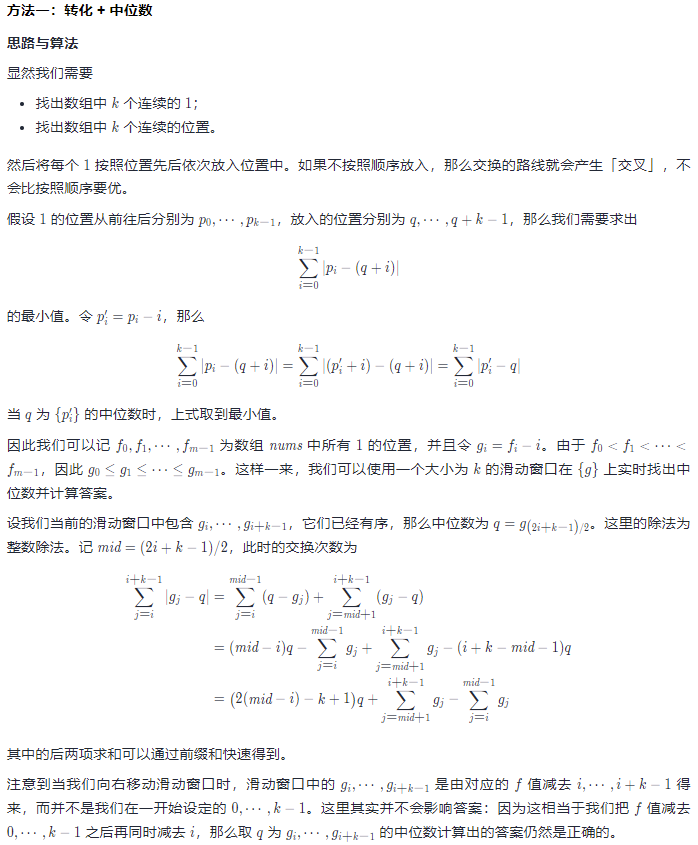
\includegraphics[width=.9\linewidth]{./pic/median.png}

\begin{minted}[fontsize=\scriptsize,linenos=false]{csharp}
public int minMoves(int[] arr, int k) {
    if (k == 1) return 0;
    int n = arr.length;
    List<Integer> g = new ArrayList<>();
    List<Integer> sum = new ArrayList<>();
    sum.add(0);
    int cnt = -1, last = 0;
    for (int i = 0; i < n; i++) {
        if (arr[i] == 0) continue;
        ++cnt;
        g.add(i-cnt);
        sum.add(last + i - cnt);
        last += i - cnt; 
    }
    int m = g.size();
    int ans = Integer.MAX_VALUE;
    for (int i = 0; i+k <= m; i++) {
        int mid = (i + i + k - 1) / 2; // 中位数下标
        int q = g.get(mid);            // 中位数
        ans = Math.min(ans, (2*(mid-i)-k+1) * q + sum.get(i+k) - sum.get(mid+1) - sum.get(mid) + sum.get(i));
    }
    return ans;
}
\end{minted}
\subsection{1838. Frequency of the Most Frequent Element - Medium}
\label{sec-6-0-8}
The frequency of an element is the number of times it occurs in an array.

You are given an integer array nums and an integer k. In one operation, you can choose an index of nums and increment the element at that index by 1.

Return the maximum possible frequency of an element after performing at most k operations.

由反证可得,在一定操作次数下最高频元素为原数组中的元素,结合贪心算法,应优先选择不大于该元素的最大数字进行递增操作。

因此,可对原数组排序后,结合双指针算法求解。设计左、右两个指针,在移动右指针的同时,维护左指针的位置,使区间内元素全部递增到右指针所在元素值的操作次数符合要求,此时区间的长度就是该元素的频率。

\begin{minted}[fontsize=\scriptsize,linenos=false]{csharp}
public int maxFrequency(int[] nums, int k) {
    int n = nums.length, ans = 1, cnt = 0;
    Arrays.sort(nums);
    for (int l = 0, r = 1; r < n; r++) {
        cnt += (nums[r] - nums[r-1]) * (r - l);// 右指针移动后所需操作次数
        while (cnt > k)                        // 操作次数超过k,移动左指针
            cnt -= nums[r] - nums[l++];
        ans = Math.max(ans, r-l+1);            // 区间长度为操作后当前元素的频数
    }
    return ans;
}
\end{minted}

\subsection{826. Most Profit Assigning Work}
\label{sec-6-0-9}
You have n jobs and m workers. You are given three arrays: difficulty, profit, and worker where:

difficulty[i] and profit[i] are the difficulty and the profit of the ith job, and
worker[j] is the ability of jth worker (i.e., the jth worker can only complete a job with difficulty at most worker[j]).
Every worker can be assigned at most one job, but one job can be completed multiple times.

For example, if three workers attempt the same job that pays \$1, then the total profit will be \$3. If a worker cannot complete any job, their profit is \$0.
Return the maximum profit we can achieve after assigning the workers to the jobs.
\begin{minted}[fontsize=\scriptsize,linenos=false]{csharp}
// 法一:暴力TreeMap---O(n^2logn)
public int maxProfitAssignment(int[] difficulty, int[] profit, int[] worker) {
    TreeMap<Integer, Integer> m = new TreeMap<>();
    for (int i = 0; i < difficulty.length; i++) 
        m.put(difficulty[i], i);
    int res = 0, idx;
    Integer low;
    for (int i = 0; i < worker.length; i++) {
        low = m.floorKey(worker[i]); // 使用treemap排序的特长
        if (low == null) continue;
        idx = m.get(low);
        for (int j = 0; j < difficulty.length; j++) 
            if (difficulty[j] <= low && profit[j] >= profit[idx])
                idx = j;
        res += profit[idx];
    }
    return res;
}
// 法二:优化的TreeMap---O(nlogn)
// 如果TreeMap里面保存的是每个difficulty[i] 对应的最大的profit,则就可以直接找floorKey对应的value就是对应的要找的value;
// 那么只需要再遍历一次TreeMap,将最大的到目前key位置最大的value放进去就行了
public int maxProfitAssignment(int[] difficulty, int[] profit, int[] worker) {
    TreeMap<Integer, Integer> m = new TreeMap<>();
    for (int i = 0; i < difficulty.length; i++) 
        m.put(difficulty[i], Math.max(m.getOrDefault(difficulty[i], 0), profit[i]));
    int max = 0;
    for (Integer key : m.keySet()) { 
        max = Math.max(max, m.get(key));
        m.put(key, max); //将最大的到目前key位置最大的value放进去
    }
    int res = 0;
    Integer low;
    for (int i = 0; i < worker.length; i++) {
        low = m.floorKey(worker[i]); // 使用treemap排序的特长
        if (low == null) continue;
        res += m.get(low);
    }
    return res;
}
// 法三:Sort + 双指针---O(nlogn)
// 思路就是先将 difficulty[]和profit组成pair,然后再将list和worker[]从小到大排序,然后遍历worker,更新tempMaxProfit,得到总的maxProfit
public int maxProfitAssignment(int[] difficulty, int[] profit, int[] worker) {
    List<int[]> list = new ArrayList<>();
    for (int i = 0; i < difficulty.length; i++) 
        list.add(new int[] {difficulty[i], profit[i]});
    Collections.sort(list, (a, b) -> {return a[0] - b[0];});
    Arrays.sort(worker);
    int res = 0, tmpMaxProfit = 0;
    // i, j同向双指针移动,更新到目前的tmpMaxProfit
    for (int i = 0, j = 0; i < worker.length; i++) {
        while (j < list.size() && list.get(j)[0] <= worker[i]) {
            tmpMaxProfit = Math.max(tmpMaxProfit, list.get(j)[1]);
            j++;
        }
        //此时tmpMaxProfit是前面所有difficulty小于worker[i]的最大的proifit
        res += tmpMaxProfit;
    }
    return res;
}
\end{minted}

\subsection{1425. Constrained Subsequence Sum - Hard}
\label{sec-6-0-10}
Given an integer array nums and an integer k, return the maximum sum of a non-empty subsequence of that array such that for every two consecutive integers in the subsequence, nums[i] and nums[j], where i < j, the condition j - i <= k is satisfied.

A subsequence of an array is obtained by deleting some number of elements (can be zero) from the array, leaving the remaining elements in their original order.

\subsection{239. Sliding Window Maximum - Hard}
\label{sec-6-0-11}
You are given an array of integers nums, there is a sliding window of size k which is moving from the very left of the array to the very right. You can only see the k numbers in the window. Each time the sliding window moves right by one position.

Return the max sliding window.

\begin{minted}[fontsize=\scriptsize,linenos=false]{csharp}
public int[] maxSlidingWindow(int[] arr, int k) {
    int n = arr.length, startWindowIdx = 0;
    ArrayDeque<Integer> q = new ArrayDeque<>(); // 维持一个递减队列
    int [] ans = new int [n - k + 1];
    for (int i = 0; i < n; i++) {
        startWindowIdx = i-k+1;
        while (!q.isEmpty() && i - q.peekFirst() >= k) q.pollFirst();     // 左出q:maintain k size window, 去头:去掉k windows之外的元素
        while (!q.isEmpty() && arr[q.peekLast()] <= arr[i]) q.pollLast(); // 右出q:去掉递减队列尾部所有不大于当前值的元素,就留一个最大值也行
        q.offerLast(i);  // 进q:进后此时q.size() == k 
        if (startWindowIdx >= 0)
            ans[startWindowIdx] = arr[q.peekFirst()]; // 使用递减队列左端最大值
    }
    return ans;
}
\end{minted}
\begin{itemize}
\item 线段树的做法
\end{itemize}
\begin{minted}[fontsize=\scriptsize,linenos=false]{csharp}
// https://blog.csdn.net/Yaokai_AssultMaster/article/details/79599809
public class MaxSeg {
    List<Integer> tree = new ArrayList<>();
    int n;
    public MaxSeg (int [] arr) {
        n = arr.length;
        tree = new ArrayList<>(2*n);
        for (int i = 0; i < n; i++) 
            tree.add(0);
        for (int i = 0; i < n; i++) 
            tree.add(arr[i]); // same effect as below
        for (int i = n-1; i >= 0; i--) // i >= 0
            tree.set(i, Math.max(tree.get(2*i), tree.get(2*i+1)));
    }
    public void update(int idx, int v) {
        idx += n;
        tree.set(idx, v);
        while (idx > 1) {
            idx /= 2;
            tree.set(idx, Math.max(tree.get(2*idx), tree.get(2*idx+1)));
        }
    }
    public int getMax(int l, int r) {
        l += n;
        r += n;
        int max = Integer.MIN_VALUE;
        while (l < r) {
            if ((l & 1) == 1) {
                max = Math.max(max, tree.get(l));
                l++;
            }
            if ((r & 1) == 1) {
                r--;            // order matters !!!
                max = Math.max(max, tree.get(r));
            }
            l >>= 1;
            r >>= 1;
        }
        return max;
    }
}
public int[] maxSlidingWindow(int[] arr, int k) {
    int n = arr.length;
    MaxSeg mat = new MaxSeg(arr);
    if (n == k) return new int [] {mat.getMax(0, n)};
    int [] res = new int [n-k+1];
    for (int i = 0; i+k <= n; i++) 
        res[i] = mat.getMax(i, i+k);
    return res;
}
\end{minted}

\subsection{双端队列:数据结构,O(N)解法类题目}
\label{sec-6-0-12}
\subsection{862. Shortest Subarray with Sum at Least K - Hard}
\label{sec-6-0-13}
Given an integer array nums and an integer k, return the length of the shortest non-empty subarray of nums with a sum of at least k. If there is no such subarray, return -1.

A subarray is a contiguous part of an array.
\begin{minted}[fontsize=\scriptsize,linenos=false]{csharp}
public int shortestSubarray(int[] nums, int k) { 
    int n = nums.length;
    int [] sum = new int[n+1];  
    for (int i = 1; i <= n; i++)  
        sum[i] = nums[i-1] + sum[i-1];
    int res = n + 1;
    ArrayDeque<Integer> q = new ArrayDeque<>(); // decreasing sum [] deque
    for (int i = 0; i <= n; i++) {
        while (!q.isEmpty() && sum[i] - sum[q.peekFirst()] >= k)  // 左出:
            res = Math.min(res, i - q.pollFirst()); // 取值了      // 取解
        while (!q.isEmpty() && sum[q.peekLast()] >= sum[i])       // 右出
            q.pollLast();  
        q.offerLast(i);                                           // 当前元素进队列
    }
    return res <= n ? res : -1;
}
\end{minted}

\subsection{1687. Delivering Boxes from Storage to Ports - Hard 滑动窗口,比较难认}
\label{sec-6-0-14}
You have the task of delivering some boxes from storage to their ports using only one ship. However, this ship has a limit on the number of boxes and the total weight that it can carry.

You are given an array boxes, where boxes[i] = [ports​​i​, weighti], and three integers portsCount, maxBoxes, and maxWeight.

ports​​i is the port where you need to deliver the ith box and weightsi is the weight of the ith box.
portsCount is the number of ports.
maxBoxes and maxWeight are the respective box and weight limits of the ship.
The boxes need to be delivered in the order they are given. The ship will follow these steps:

The ship will take some number of boxes from the boxes queue, not violating the maxBoxes and maxWeight constraints.
For each loaded box in order, the ship will make a trip to the port the box needs to be delivered to and deliver it. If the ship is already at the correct port, no trip is needed, and the box can immediately be delivered.
The ship then makes a return trip to storage to take more boxes from the queue.
The ship must end at storage after all the boxes have been delivered.

Return the minimum number of trips the ship needs to make to deliver all boxes to their respective ports.
\begin{enumerate}
\item 解题思路与分析: 滑动窗口
\label{sec-6-0-14-1}
\begin{itemize}
\item 这里会需要一种决策:需要总运送次数最少,就涉及到同一船是否只装送往同一个港口的优化与选择问题,用滑动窗口,也有贪心的解法
\item 时间复杂度: O(N)
\end{itemize}
\begin{minted}[fontsize=\scriptsize,linenos=false]{csharp}
public int boxDelivering(int[][] box, int __, int max, int limit) {
    int n = box.length;
    int[] dp = new int[n+1]; // Minimum trips for first n boxes.
    int wit = 0, cost = 2;   // cumulative weight, cumulative cost
    int l = 0;                   // left ptr
    for (int r = 0; r < n; r++) {// right ptr
        wit += box[r][1];
        if (r > 0 && box[r][0] != box[r-1][0]) cost++; // 现箱子与上一个箱子运往的目的地不同
        /* drop box iff:
           - There are too many box (r-l >= max)
           - The box are too heavy (weight > limit)
           - It is redundant to carry them (dp[l] == dp[l+1]).
        */                                 // 送往同一个港口的箱子向右滑动,直到改变消耗的临界点
        while (r - l >= max || wit > limit || (l < r && dp[l] == dp[l+1])) { // 滑动窗口:左窗口右移
            wit -= box[l][1];
            if (box[l+1][0] != box[l][0]) cost--;
            l++;
        }
        dp[r+1] = cost + dp[l]; // 运完下标为 r 的箱子后的最小次数,对应 dp[r+1]
    }
    return dp[n];
}
\end{minted}
\begin{itemize}
\item 一种dp的写法,写得天外来仙,可惜不是很好懂
\end{itemize}
\begin{minted}[fontsize=\scriptsize,linenos=false]{csharp}
public int boxDelivering(int [][] box, int portsCount, int maxBox, int maxWeight) {
    int n = box.length, j = 0, lastj = 0, cnt = 0; // cnt: cost
    int [] dp = new int [n+1];
    Arrays.fill(dp, Integer.MAX_VALUE / 2);
    dp[0] = 0;
    for (int i = 0; i < n; i++) {
        while (j < n && maxBox > 0 && maxWeight >= box[j][1]) {
            maxBox -= 1;
            maxWeight -= box[j][1];
            if (j == 0 || box[j][0] != box[j-1][0]) {
                lastj = j; // 新目的地港口的第一个下标
                cnt++; // 增加消耗
            }
            ++j; // keep expanding the right pointer when we can 右窗口尽可能地向右延伸:只要有空间,延伸至最远
        }
        dp[j] = Math.min(dp[j], dp[i] + cnt + 1);
        dp[lastj] = Math.min(dp[lastj], dp[i] + cnt);
        // 随着i的增加,左窗口右移:移走第i个箱子所腾出的空间(箱子个安数、重量,以及潜在可能减少的一次消耗)都需要更新
        maxBox += 1; // now as we move the left pointer i forward (don't put the ith box in this trip),
        maxWeight += box[i][1];  // we increase the number of available boxes and available weights
        if (i == n-1 || box[i][0] != box[i+1][0]) cnt--;
    }
    return dp[n];
}
\end{minted}
\end{enumerate}

\subsection{992. Subarrays with K Different Integers - Hard}
\label{sec-6-0-15}
Given an integer array nums and an integer k, return the number of good subarrays of nums.

A good array is an array where the number of different integers in that array is exactly k.

For example, [1,2,3,1,2] has 3 different integers: 1, 2, and 3.
A subarray is a contiguous part of an array.
\begin{enumerate}
\item 解题思路与分析
\label{sec-6-0-15-1}
\begin{itemize}
\item 思路依然是滑动窗口,但是这一题是没法直接套用76题的模板的,有一些变动(引用)。回忆前面做的滑动窗口的题目,有求过子数组里面最多K个不同元素的题(340),所以这个解法的思路是求子数组里面最多K个不同元素的子数组的数量 - 子数组里面最多K - 1个不同元素的子数组的数量。
\end{itemize}
\begin{minted}[fontsize=\scriptsize,linenos=false]{csharp}
private int atMostK(int [] arr, int k) {
    int ans = 0, l = 0;                    // Left boundary of window
    Map<Integer, Integer> cnt = new HashMap<>(); // Map to keep track of number of distinct elements in the current window
    for (int i = 0; i < arr.length; i++) { // i : right
        cnt.put(arr[i], cnt.getOrDefault(arr[i], 0) + 1);
        while (cnt.size() > k) {
            if (cnt.get(arr[l]) > 1) cnt.put(arr[l], cnt.get(arr[l])-1);
            else cnt.remove(arr[l]);
            l++;
        }
        ans += i - l + 1; // Adding the count of subarrays with at most K distinct elements in the current window
    }
    return ans;
}
public int subarraysWithKDistinct(int[]arr, int k) {
    return atMostK(arr, k) - atMostK(arr, k-1);
}
\end{minted}
\end{enumerate}

\subsection{1438. Longest Continuous Subarray With Absolute Diff Less Than or Equal to Limit - Medium 双端队列}
\label{sec-6-0-16}
Given an array of integers nums and an integer limit, return the size of the longest non-empty subarray such that the absolute difference between any two elements of this subarray is less than or equal to limit.
\begin{enumerate}
\item 解题思路与分析
\label{sec-6-0-16-1}
\begin{itemize}
\item 如果使用普通列表再排序的话会增加一个logn的时间复杂度,会超时!
\item 选对了数据类型后,直接套滑窗模板即可,简单的一。。。
\item Intuition:
\end{itemize}
\begin{minted}[fontsize=\scriptsize,linenos=false]{csharp}
 . we can use siliding window but we need to keep track of minimum and maximum in every window 
 . treemap can be used for this purpose to keep track of min and max both
\end{minted}
\begin{itemize}
\item 这是一种临场应对的偷懒解法,选对数据结构,牺牲一点儿效率,但是可以最大限度地保证结果的正确性
\end{itemize}
\begin{minted}[fontsize=\scriptsize,linenos=false]{csharp}
// Time complexity: O(N*LogN), insertion in treeMap is logN and for N elements it is O(N*LogN)
// Auxiliary Space: O(N), every key enters the map once and in worst case every key can be present with frequency one
public int longestSubarray(int[] arr, int limit) { // TreeMap to keep Min & Max at O(NlogN)
    TreeMap<Integer, Integer> cnt = new TreeMap<>();
    int l = 0, r = 0;
    while (r < arr.length) {
        cnt.put(arr[r], cnt.getOrDefault(arr[r], 0) + 1);
        if (cnt.lastEntry().getKey() - cnt.firstEntry().getKey() > limit) {
            if (cnt.get(arr[l]) > 1)
                cnt.put(arr[l], cnt.get(arr[l])-1);
            else cnt.remove(arr[l]);
            l++;
        }
        r++;
    }
    return r - l; // 这样维护的就是全局最优解了?!!!
}
\end{minted}
\begin{itemize}
\item 但是在平时练习时,还是要不断地寻求最优解,使用双端队列,得O(N)线性复杂度
\item Intuition:
\end{itemize}
\begin{minted}[fontsize=\scriptsize,linenos=false]{csharp}
// . we can use siliding window but we need to keep track of minimum and maximum in every window 
// . 2 Deques can be used for this purpose to keep track of min and max.
// Time complexity: O(N), N is number of elements in nums
// Auxiliary Space: O(N)
public int longestSubarray(int[] nums, int limit) { // 双端队列:从右边加入
    ArrayDeque<Integer> min = new ArrayDeque<>();   // 单调递增队列: 左小右大
    ArrayDeque<Integer> max = new ArrayDeque<>();   // 单调递减队列: 左大右小
    int l = 0, r = 0, ans = 0;
    while (r < nums.length) {
        int rval = nums[r];
//to ensure that minQ have minimum element as head             
        while (!min.isEmpty() && min.peekLast() > rval) min.pollLast(); // 维护:右边,比当前待入列值大的,全扔出去
//to ensure that maxQ have maximum element as head                
        while (!max.isEmpty() && max.peekLast() < rval) max.pollLast(); // 维护:右边,比当前待入列值小的,全扔出去                
        min.offerLast(rval); // 入队列,从右边加入
        max.offerLast(rval); // 
//In case max-min is greater than the limit slide the left side or window         
        if (max.peekFirst() - min.peekFirst() > limit) {     // 维护合法窗口范围: 会两个队列都把 l 下标的值抓不出去吗?
            if (min.peekFirst() == nums[l]) min.pollFirst(); // 
            if (max.peekFirst() == nums[l]) max.pollFirst(); // 
            l++;
        }
        r++;
    }
    return r - l;
}
\end{minted}
\begin{itemize}
\item 另一种把它"刷"过去的应付的写法(MinSeg, MaxSeg列在这里,方便自己以后参考时查找)
\end{itemize}
\begin{minted}[fontsize=\scriptsize,linenos=false]{csharp}
public class MaxSeg {
    List<Integer> tree = new ArrayList<>();
    int n;
    public MaxSeg (int [] arr) {
        n = arr.length;
        tree = new ArrayList<>(2 * n);
        for (int i = 0; i < n; i++)
            tree.add(0);
        for (int i = 0; i < n; i++)
            tree.add(arr[i]); // same effect as below
        for (int i = n-1; i >= 0; i--) // i >= 0
            tree.set(i, Math.max(tree.get(2 * i), tree.get(2 * i+1)));
    }
    public void update(int idx, int v) {
        idx += n;
        tree.set(idx, v);
        while (idx > 1) {
            idx /= 2;
            tree.set(idx, Math.max(tree.get(2 * idx), tree.get(2 * idx+1)));
        }
    }
    public int getMax(int l, int r) {
        l += n;
        r += n;
        int max = Integer.MIN_VALUE;
        while (l < r) {
            if ((l & 1) == 1) {
                max = Math.max(max, tree.get(l));
                l++;
            }
            if ((r & 1) == 1) {
                r--; // order matters !!!
                max = Math.max(max, tree.get(r));
            }
            l >>= 1;
            r >>= 1;
        }
        return max;
    }
}        
public class MinSeg {
    List<Integer> tree = new ArrayList<>();
    int n;
    public MinSeg (int [] arr) {
        n = arr.length;
        tree = new ArrayList<>(2*n);
        for (int i = 0; i < n; i++) 
            tree.add(0);
        for (int i = 0; i < n; i++) 
            tree.add(arr[i]); 
        for (int i = n-1; i >= 0; i--)  // i >= 0
            tree.set(i,  Math.min(tree.get(2*i),  tree.get(2*i+1)));
    }
    public void update(int idx,  int v) {
        idx += n;
        tree.set(idx,  v);
        while (idx > 1) {
            idx /= 2;
            tree.set(idx,  Math.min(tree.get(2*idx),  tree.get(2*idx+1)));
        }
    }
    public int getMin(int l,  int r) { // [l, r) include left, not included right
        l += n;
        r += n;
        int min = Integer.MAX_VALUE;
        while (l < r) {
            if ((l & 1) == 1) {
                min = Math.min(min,  tree.get(l));
                l++;
            }
            if ((r & 1) == 1) {
                r--; // order matters !!!
                min = Math.min(min,  tree.get(r));
            }
            l >>= 1;
            r >>= 1;
        }
        return min;
    }
}
public int longestSubarray(int[] arr, int limit) { // 单调递增队列,左小右大,右进左出 
    MaxSeg max = new MaxSeg(arr);
    MinSeg min = new MinSeg(arr);
    int res = 0, tmp = 0, j = 0;
    int n = arr.length;
    for (int i = 1; i <= n; i++) {
        if (max.getMax(j, i) - min.getMin(j, i) <= limit) {
            tmp = i-j;
            res = Math.max(res, tmp);
        } else 
            while (max.getMax(j, i) - min.getMin(j, i) > limit && j < i) ++j;
    }
    return res;
}
\end{minted}
\end{enumerate}
\subsection{1493. Longest Subarray of 1's After Deleting One Element - Medium}
\label{sec-6-0-17}
Given a binary array nums, you should delete one element from it.

Return the size of the longest non-empty subarray containing only 1's in the resulting array. Return 0 if there is no such subarray.
\begin{enumerate}
\item 解题思路与分析: 滑动窗口 O(N)
\label{sec-6-0-17-1}

是滑动窗口的题目,以后比赛的时候就这么写,自己数下标,数得累死还bug满天飞,借助一个双端队列,至少自动过滤掉不少bug

\begin{minted}[fontsize=\scriptsize,linenos=false]{csharp}
public int longestSubarray(int[] a) {
    int n = a.length, cnt = 0, i = 0, max = 0;
    ArrayDeque<Integer> q = new ArrayDeque<>();
    boolean hasO = false; // {0, 0, 1, 1} 这个特例不能忘记了
    while (i < n && a[i] == 0) {
        hasO = true;
        i++;
    }
    if (i == n) return 0;
    for (; i < n; i++) {
        q.offerLast(a[i]);
        if (a[i] == 0) {
            cnt++;
            if (cnt == 2) {
                max = Math.max(max, q.size()-cnt);
                while (!q.isEmpty() && q.peek() != 0) q.pollFirst();
                q.pollFirst();
                cnt--;
            }
        }
    }
    if (a[n-1] == 1) max = Math.max(max, q.size()-(cnt > 0 ? cnt : (hasO ? 0 : 1)));
    else max = Math.max(max, q.size()-cnt);
    return max;
}
\end{minted}
\begin{itemize}
\item 贴个别人真正的滑动窗口的代码
\end{itemize}
\begin{minted}[fontsize=\scriptsize,linenos=false]{cpp}
int longestSubarray(vector<int>& nums) {
    const int n = nums.size();
    int ans = 0;
    int sum = 0; // sum of nums[l~r].
    for (int l = 0, r = 0; r < n; ++r) {
        sum += nums[r];
        while (l < r && sum < r - l) // Maintain sum >= r - l, at most 1 zero.
            sum -= nums[l++];
        ans = max(ans, r - l);
    }
    return ans;
}
\end{minted}
\item 解题思路与分析: 双变量
\label{sec-6-0-17-2}

早上的时候不是刚写过一个这样的题吗 ? 与926 的第二种解法有什么区别? 

\begin{minted}[fontsize=\scriptsize,linenos=false]{csharp}
// count1:当前包含一个非1的连续长度。
// count2:当前全是1的连续长度。
// 循环数组每一个数字,如果当前数字是1,count1和count2同时加一,同时使用count1更新全局最大值。
// 重点来了,如果当前数字是非1,则设count1等于count2,count2设为0。最后处理一下全是1的特例即可。
public int longestSubarray(int[] a) { // bug出多了,自己也能悟出来:数据结构帮大忙:
    int n = a.length, ans = 0, cnt = 0, one = 0, zoo = 0;
    for (Integer v : a) {
        if (v == 0) {
            zoo++;
            cnt = one;
            one = 0;
        } else {
            cnt++;
            one++;
            ans = Math.max(ans, cnt);
        }
    }
    return ans == n ? n-1 : ans;
}
\end{minted}
\item 解题思路与分析: DP
\label{sec-6-0-17-3}
Preprocess:

l[i] := longest 1s from left side ends with nums[i], l[i] = nums[i] + nums[i] * l[i – 1]

r[i] := longest 1s from right side ends with nums[i], r[i] = nums[i] + nums[i] * r[i + 1]

Use each node as a bridge (ignored), the total number of consecutive 1s = l[i – 1] + r[i + 1].

ans = max\{l[i-1] + r[i +1]\}

Time complexity: O(n)

Space complexity: O(n)
\begin{minted}[fontsize=\scriptsize,linenos=false]{cpp}
int longestSubarray(vector<int>& nums) {
    const int n = nums.size();
    vector<int> l(n);
    vector<int> r(n);
    for (int i = 0; i < n; ++i)
        l[i] = (i > 0 ? l[i - 1] * nums[i] : 0) + nums[i];
    for (int i = n - 1; i >= 0; --i)
        r[i] = (i < n - 1 ? r[i + 1] * nums[i] : 0) + nums[i];
    int ans = 0;
    for (int i = 0; i < n; ++i)
        ans = max(ans, (i > 0 ? l[i - 1] : 0) + 
                       (i < n - 1 ? r[i + 1] : 0));
    return ans;
}
\end{minted}
\item 解题思路与分析
\label{sec-6-0-17-4}
\begin{minted}[fontsize=\scriptsize,linenos=false]{csharp}
dp[i][0] := longest subarray ends with nums[i] has no ones.
dp[i][0] := longest subarray ends with nums[i] has 1 one.
if nums[i] == 1:
dp[i][0] = dp[i – 1][0] + 1
dp[i][1] = dp[i – 1][1] + 1
if nums[i] == 0:
dp[i][0] = 0
dp[i][1] = dp[i – 1][0] + 1
\end{minted}

Time complexity: O(n)

Space complexity: O(n) -> O(1)

\begin{minted}[fontsize=\scriptsize,linenos=false]{cpp}
int longestSubarray(vector<int>& nums) {
    const int n = nums.size();
    // dp[i][0] := longest subarray ends with nums[i-1] has no zeros.
    // dp[i][0] := longest subarray ends with nums[i-1] has 1 zero.
    vector<vector<int>> dp(n + 1, vector<int>(2));
    int ans = 0;
    for (int i = 1; i <= n; ++i) {
        if (nums[i - 1] == 1) {
            dp[i][0] = dp[i - 1][0] + 1;
            dp[i][1] = dp[i - 1][1] + 1;
        } else {
            dp[i][0] = 0;
            dp[i][1] = dp[i - 1][0] + 1;
        }
        ans = max({ans, dp[i][0] - 1, dp[i][1] - 1});
    }
    return ans;
}
\end{minted}
\end{enumerate}

\subsection{857. Minimum Cost to Hire K Workers - Hard}
\label{sec-6-0-18}
There are n workers. You are given two integer arrays quality and wage where quality[i] is the quality of the ith worker and wage[i] is the minimum wage expectation for the ith worker.

We want to hire exactly k workers to form a paid group. To hire a group of k workers, we must pay them according to the following rules:

Every worker in the paid group should be paid in the ratio of their quality compared to other workers in the paid group.
Every worker in the paid group must be paid at least their minimum wage expectation.
Given the integer k, return the least amount of money needed to form a paid group satisfying the above conditions. Answers within 10-5 of the actual answer will be accepted.
\begin{enumerate}
\item 解题思路与分析
\label{sec-6-0-18-1}
\begin{itemize}
\item 做题的时候没有想明白,为什么不是性价比最低的k个工人,什么情况下性价比最低的k个工人不是题目要求的答案?
\item 时间复杂度O ( n log ⁡ n ),空间O ( n ) 。
\end{itemize}
\begin{minted}[fontsize=\scriptsize,linenos=false]{csharp}
public double mincostToHireWorkers(int[] quality, int[] wage, int k) {
    int n = quality.length;
    List<int []> l = new ArrayList<>();
    for (int i = 0; i < n; i++) {
        int [] cur = new int [] {wage[i], quality[i]};
        l.add(cur);
    }
    Collections.sort(l, (a, b) -> Double.compare((double)a[0] / a[1], (double)b[0] / b[1]));
    Queue<Integer> q = new PriorityQueue<>((x, y) -> -Integer.compare(x, y)); // 堆里存所以t值小于等于当前枚举的t值的工人中,q值最小的k个人的q值
    double res = 1e18, sum = 0;
    for (int i = 0; i < n; i++) {
        int [] cur = l.get(i);
        sum += cur[1];
        q.offer(cur[1]);
        if (q.size() > k)
            sum -= q.poll();
        if (q.size() == k)
            res = Math.min(res, sum * (double)cur[0] / (double)cur[1]);
    }
    return res;
}
\end{minted}
\end{enumerate}

\subsection{480 Sliding Window Median}
\label{sec-6-0-19}
The median is the middle value in an ordered integer list. If the size of the list is even, there is no middle value. So the median is the mean of the two middle values.
For examples, if arr = [2,3,4], the median is 3.
For examples, if arr = [1,2,3,4], the median is (2 + 3) / 2 = 2.5.
You are given an integer array nums and an integer k. There is a sliding window of size k which is moving from the very left of the array to the very right. You can only see the k numbers in the window. Each time the sliding window moves right by one position.
Return the median array for each window in the original array. Answers within 10-5 of the actual value will be accepted.
\begin{minted}[fontsize=\scriptsize,linenos=false]{csharp}
public double[] medianSlidingWindow(int[] nums, int k) {
    TreeMap<Integer, Integer> ma = new TreeMap<>();
    TreeMap<Integer, Integer> mb = new TreeMap<>();
    for (int i = 0; i < k; i++) {
        if (i % 2 == 0) {
            mb.put(nums[i], mb.getOrDefault(nums[i], 0) + 1);
            int n = mb.firstKey();
            if (mb.get(n) == 1) mb.remove(n);
            else mb.put(n, mb.get(n) - 1);
            ma.put(n, ma.getOrDefault(n, 0) + 1);
        } else {
            ma.put(nums[i], ma.getOrDefault(nums[i], 0) + 1);
            int n = ma.lastKey();
            if (ma.get(n) == 1) ma.remove(n);
            else ma.put(n, ma.get(n) - 1);
            mb.put(n, mb.getOrDefault(n, 0) + 1);
        }
    }
    double [] res = new double[nums.length-k+1];
    if (k % 2 == 1) res[0] = ma.lastKey();
    else res[0] =  (double)(((long)(ma.lastKey()) + (long)(mb.firstKey())) / 2.0);
    for (int i = 0; i + k < nums.length; i++) {
        ma.put(nums[i+k], ma.getOrDefault(nums[i+k], 0) + 1);
        int n = ma.lastKey();
        if (ma.get(n) == 1) ma.remove(n);
        else ma.put(n, ma.get(n) - 1);
        mb.put(n, mb.getOrDefault(n, 0) + 1);
        if (ma.containsKey(nums[i])) {
            if (ma.get(nums[i]) == 1) ma.remove(nums[i]);
            else ma.put(nums[i], ma.get(nums[i]) - 1);
            int v = mb.firstKey();
            if (mb.get(v) == 1) mb.remove(v);
            else mb.put(v, mb.get(v) - 1);
            ma.put(v, ma.getOrDefault(v, 0) + 1);
        } else {
            if (mb.get(nums[i]) == 1) mb.remove(nums[i]);
            else mb.put(nums[i], mb.get(nums[i]) - 1);
        }
        if (k % 2 == 1) res[i+1] = ma.lastKey();
        else res[i+1] = (double)(((long)(ma.lastKey()) + (long)(mb.firstKey())) / 2.0);
    }
    return res;
}
\end{minted}

\chapter{TreeMap}
\label{sec-7}
\section{2382. Maximum Segment Sum After Removals - Hard}
\label{sec-7-1}
You are given two 0-indexed integer arrays nums and removeQueries, both of length n. For the ith query, the element in nums at the index removeQueries[i] is removed, splitting nums into different segments.

A segment is a contiguous sequence of positive integers in nums. A segment sum is the sum of every element in a segment.

Return an integer array answer, of length n, where answer[i] is the maximum segment sum after applying the ith removal.

Note: The same index will not be removed more than once.
\subsection{思路分析}
\label{sec-7-1-1}
\begin{itemize}
\item Using simple logic of storing the ranges and splitting them as solving the query.
\item Intially, we will be having whole array as are range (0, n-1). Now as we solve queries, say remove index x or set index x value as 0, we will split our range into (0, x -1) and (x + 1, n). Also, we will remove our previous range as it is of no use.
\item There can be cases in that, suppose we need to remove x and there is range (x, x), then we will simple remove it and not adding anything back (refer code below)
\item Now, to get the maximum sum of all the possible ranges, we will use another treemap, which will store sum to its frequency (frequency because multiple ranges can have same sum). And we can fetch maximum sum at any point in O(1) by simple getting last element of treemap.
\end{itemize}
\begin{minted}[fontsize=\scriptsize,linenos=false]{csharp}
public long[] maximumSegmentSum(int[] a, int[] q) {
    int n = a.length;
    long [] sum = new long [n+1], ans = new long [n];
    for (int i = 0; i < n; i++) // calc preSum
        sum[i+1] = sum[i] + a[i];
    TreeMap<int [], Long> m = new TreeMap<>((x, y)->x[0] - y[0]); // 这里定义了一个相对独特的比较方式  ranges
    // TreeMap to store all the possible sums of range we encounter while solving queries, we are storing frequencies because 
    // multiple range can have same sum.            
    TreeMap<Long, Integer> sums = new TreeMap<>(); 
    m.put(new int [] {0, n-1}, sum[n]);
    sums.put(sum[n], 1);
    for (int i = 0; i < n; i++) {
        int v = q[i];
        // finding range which will split when node index is removed or set 0.                
        int [] rangeToBeRemoved = m.floorKey(new int [] {v}); // 所以数组的长短都没有关系
        Long sumv =m.get(rangeToBeRemoved);
        // removing/ reducing sum from sums Map because we are splitting that range, so it is no longer valid
        int freq = sums.get(sumv);
        if (freq == 1) sums.remove(sumv);
        else sums.put(sumv, freq-1);
        m.remove(rangeToBeRemoved); // removing that range
        int l = rangeToBeRemoved[0], r = rangeToBeRemoved[1];
        long curSum = 0;
        // Splitting range and store back new ranges form along with its sum.
        if (l == v && r != v) { // 更新当前分割点右边的片段
            curSum = sum[r+1] - sum[v+1];
            m.put(new int [] {v+1, r}, curSum);
            sums.put(curSum, sums.getOrDefault(curSum, 0) + 1);
        } else if (l != v && r == v) { // 更新当前分割点左边的片段
            curSum = sum[v] - sum[l];
            m.put(new int [] {l, v-1}, curSum);
            sums.put(curSum, sums.getOrDefault(curSum, 0) + 1);
        } else if (l < v && r > v) {
            // 左边
            curSum = sum[v] - sum[l];
            m.put(new int [] {l, v-1}, curSum);
            sums.put(curSum, sums.getOrDefault(curSum, 0) + 1);
            // 右边
            curSum = sum[r+1] - sum[v+1];
            m.put(new int [] {v+1, r}, curSum);
            sums.put(curSum, sums.getOrDefault(curSum, 0) + 1);
        }
        if (sums.size() !=  0)
            ans[i] = sums.lastKey();
    }
    return ans;
}
\end{minted}
\begin{itemize}
\item 另外一个想起来相对简单的思路
\begin{minted}[fontsize=\scriptsize,linenos=false]{csharp}
public long[] maximumSegmentSum(int[] a, int[] qr) {
    int n = a.length;
    Queue<long []> q = new PriorityQueue<>((x, y) -> x[2] <= y[2] ? 1 : -1); // 转化成int值
    TreeSet<Integer> s = new TreeSet<>();
    long [] sum = new long [n], ans = new long [n];
    s.add(-1); // qr[i] in range [0, n)
    s.add(n);
    for (int i = 0; i < n; i++) {
        sum[i] = a[i];
        if (i > 0) sum[i] += sum[i-1];
    }
    q.offer(new long [] {0, n-1, sum[n-1]}); // [ bgn, end ], sum of segment
    for (int i = 0; i < n; i++) {
        int v = qr[i];
        s.add(v);
// 先添加可能会产生的分割点左右的两个新片段;再从QUEUE里移除含有当前分割点的一个片段,或是直接读最大有效值                
        // l, r: left, right, 比当前分割点小的最大值,和比当前分割点大的最小值
        int l = s.lower(v), r = s.higher(v); 
        if (l + 1 < v) // 比当前分割点小的可以产生段新的片段
            q.offer(new long [] {(long)l + 1, (long)v - 1, sum[v-1] - (long)(l == -1 ? 0 : sum[l])}); // - sum[l]
        if (v + 1 < r) // 比当前分割点大的也可以产生一段新的片段
            q.offer(new long [] {(long)v+1, (long)r-1, sum[r-1] - sum[v]}); // - sum[v]
        while (!q.isEmpty()) {
            long [] cur = q.peek();
            int bgn = (int)cur[0], end = (int)cur[1];
            // 根据当前片段的两个端点值来确认:当前片段是有效片段,取第一个有效片段读值
            if (s.higher(bgn-1) > end) {
                ans[i] = q.peek()[2];
                break;
            } else q.poll(); // 如果是无效片段,就把它扔掉
        }
    }
    return ans;
}
\end{minted}
\end{itemize}
\chapter{HashMap}
\label{sec-8}
\subsection{数有多少个数组数不清楚}
\label{sec-8-0-1}
\subsection{1392. Longest Happy Prefix - Hard KMP算法 - 这个题需要重写}
\label{sec-8-0-2}
A string is called a happy prefix if is a non-empty prefix which is also a suffix (excluding itself).

Given a string s, return the longest happy prefix of s. Return an empty string "" if no such prefix exists.
\begin{minted}[fontsize=\scriptsize,linenos=false]{csharp}
// 频繁的字符串操作(substring和equals操作)会大幅消耗执行时间,也会导致TLE时间超时。
// 因此我们可以使用字符串的hash值方式来比较前后缀是否相同。这里我们需要普及一个知识点,任意一个字符串的Hash值的计算公式为:
// int hash=s[0]∗31^(n−1)+s[1]∗31^(n−2) +...+s[n−2]∗31^1+s[n−1]∗31^0
//     对于前缀hash,每次长度加一后hash的变化应该是:
//     hash = hash*31 + 新添头字符ch
//     对于后缀hash,每次长度加一后hash的变化应该是:
//     hash = hash + 新添尾字符*31^t   (t为后缀长度减1)
//     这样我们每次只需要比较前缀hash与后缀hash是否相同即可。
public String longestPrefix(String s) {
    int n = s.length(), hashPre = 0, hashSuf = 0;
    int left = 0, right = n-1, pow = 1, maxLen = 0;
    String res = "";
    while (left < n-1) {
        hashPre = hashPre * 31 + s.charAt(left);
        hashSuf = hashSuf + s.charAt(right)*pow;
        if (hashPre == hashSuf) maxLen = left + 1;
        left ++;
        right --;
        pow *= 31;
    }
    return maxLen == 0 ? "" : s.substring(0, maxLen);
}
\end{minted}
\begin{enumerate}
\item 解题思路与分析
\label{sec-8-0-2-1}
\begin{itemize}
\item 利用字典wmap保存单词 -> 下标的键值对
\item 遍历单词列表words,记当前单词为word,下标为idx:
\end{itemize}
\begin{minted}[fontsize=\scriptsize,linenos=false]{csharp}
1). 若当前单词word本身为回文,且words中存在空串,则将空串下标bidx与idx加入答案
2). 若当前单词的逆序串在words中,则将逆序串下标ridx与idx加入答案
3). 将当前单词word拆分为左右两半left,right。
     3.1) 若left为回文,并且right的逆序串在words中,则将right的逆序串下标rridx与idx加入答案
     3.2) 若right为回文,并且left的逆序串在words中,则将left的逆序串下标idx与rlidx加入答案
\end{minted}

情况分析清楚以后,针对每个情况逐个判断, 然后提前建好hashmap以后判断就好。

细节部分是不要忘记空字符串的情况, 然后针对整个字符串反过来的情况,不要有重复。
\begin{minted}[fontsize=\scriptsize,linenos=false]{csharp}
private boolean isPalindrome(String s, int i, int j) {
    while (i < j) 
        if (s.charAt(i++) != s.charAt(j--)) return false;
    return true;
}
public List<List<Integer>> palindromePairs(String[] words) {
    Map<String, Integer> map = new HashMap<>();
    List<List<Integer>> ans = new ArrayList<>();
    for (int i = 0; i < words.length; i++) 
        map.put(words[i], i);
    for (int i = 0; i < words.length; i++) {
        if (words[i].equals("")) {
            for (int j = 0; j < words.length; j++) {
                String w = words[j];
                if (isPalindrome(w, 0, w.length()-1) && j != i) {
                    ans.add(List.of(i, j));
                    ans.add(List.of(j, i));
                }
            }
            continue;
        }
        StringBuilder sb = new StringBuilder(words[i]);
        sb.reverse();
        String bw = sb.toString();
        if (map.containsKey(bw)) {
            int res = map.get(bw);
            if (res != i) ans.add(List.of(i, res));
        }
        for (int j = 1; j < bw.length(); j++) {
            if (isPalindrome(bw, 0, j-1)) {
                String s = bw.substring(j);
                if (map.containsKey(s))
                    ans.add(List.of(i, map.get(s)));
            }
            if (isPalindrome(bw, j, bw.length()-1)) {
                String s = bw.substring(0, j);
                if (map.containsKey(s))
                    ans.add(List.of(map.get(s), i));
            }
        }
    }
    return ans;
}
\end{minted}

\item KMP 算法
\label{sec-8-0-2-2}
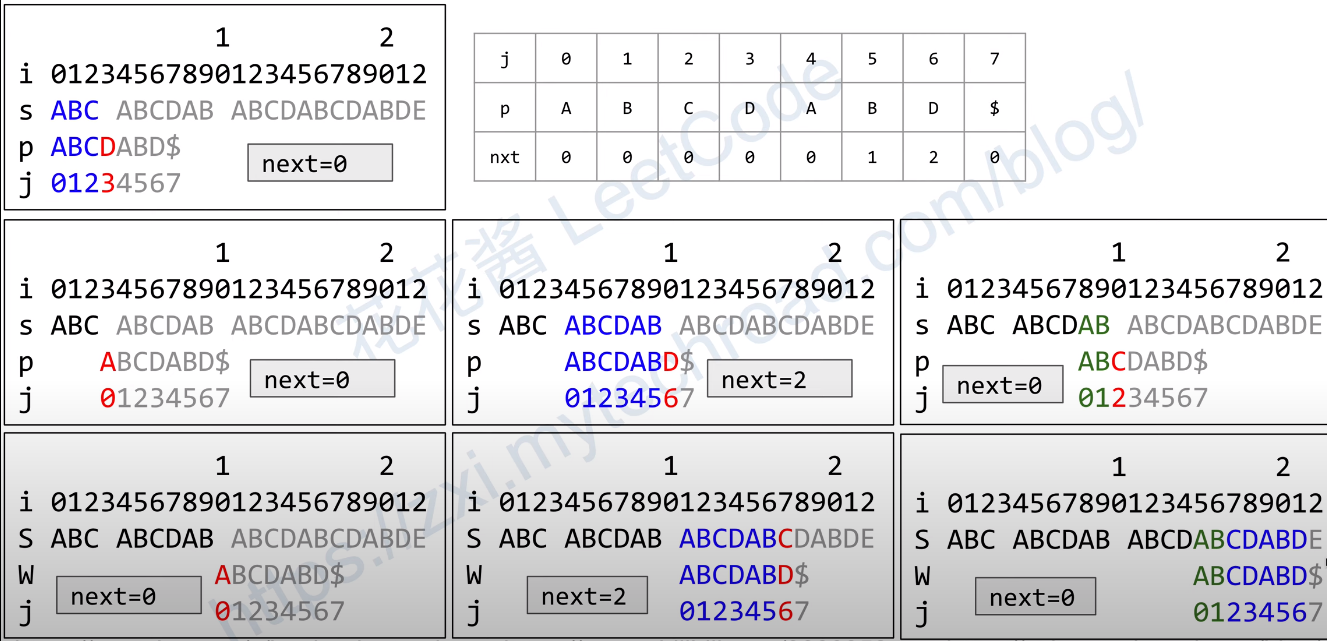
\includegraphics[width=.9\linewidth]{./pic/kmp.png}

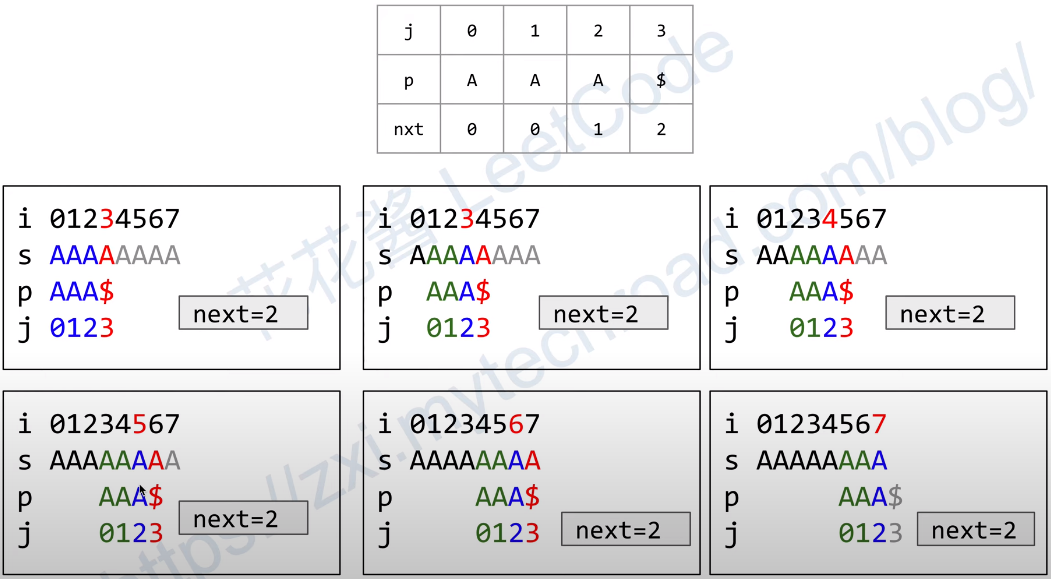
\includegraphics[width=.9\linewidth]{./pic/kmp2.png}

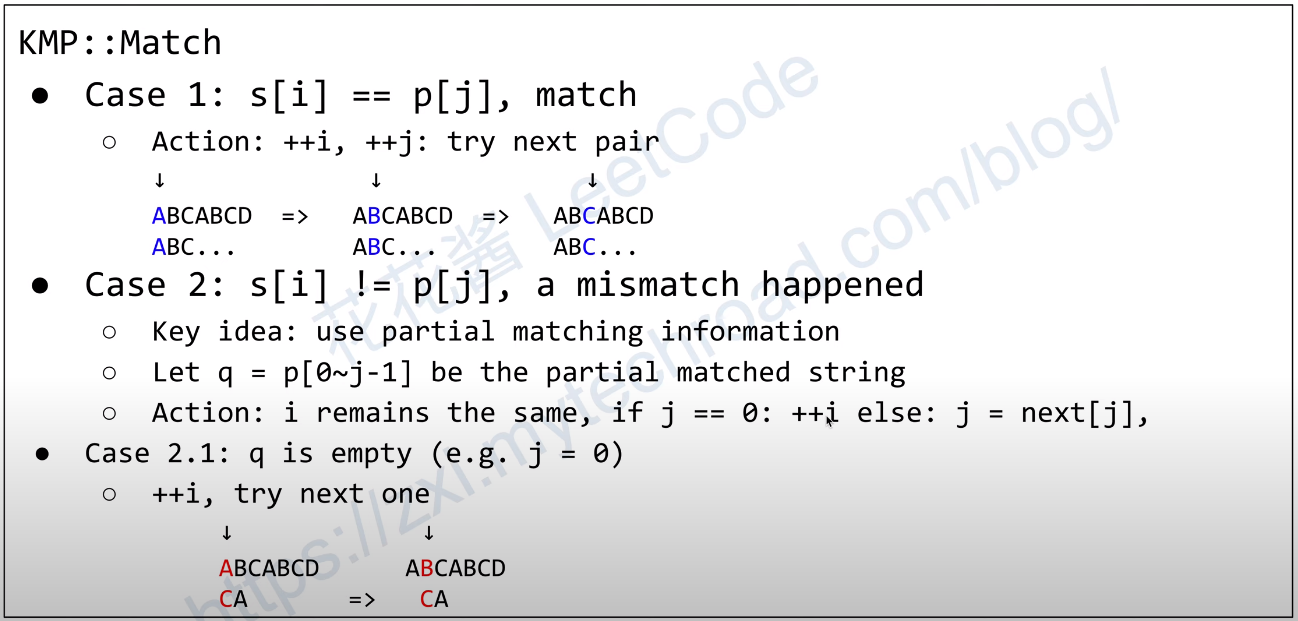
\includegraphics[width=.9\linewidth]{./pic/kmp3.png}

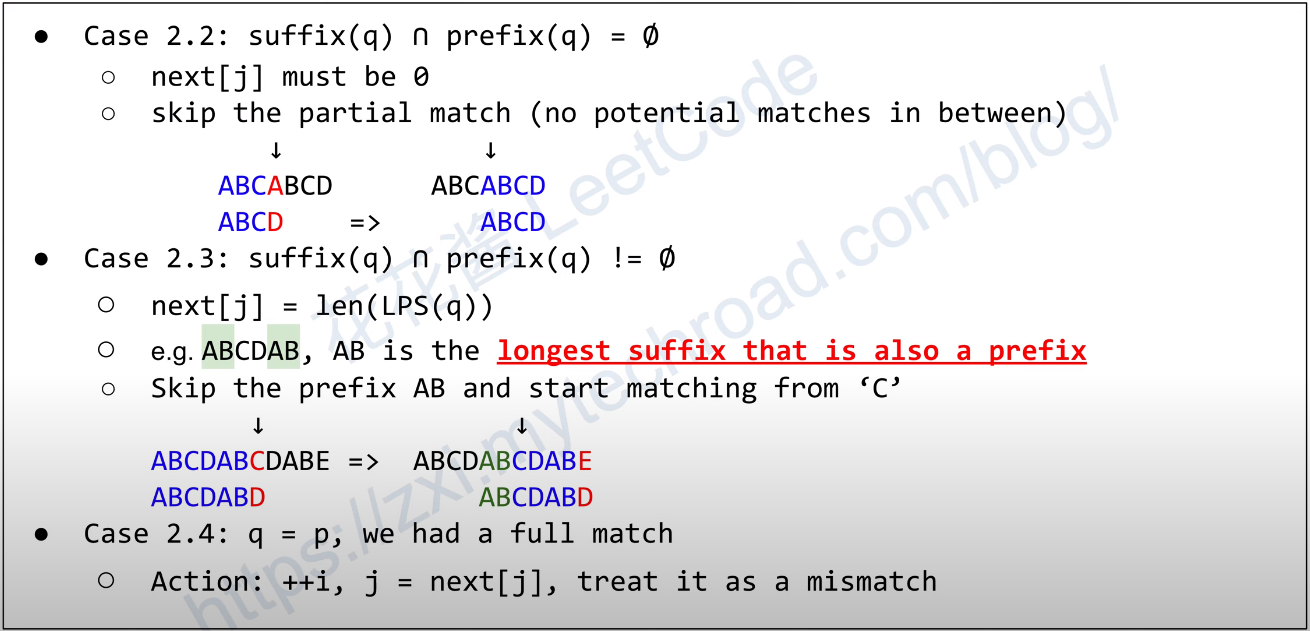
\includegraphics[width=.9\linewidth]{./pic/kmp4.png}

\begin{minted}[fontsize=\scriptsize,linenos=false]{csharp}
// straight forward KMP algorithm - 8ms - beats 94% time - O(N) time and O(N) space
public String longestPrefix(String s) {
    int i, x, N = s.length();
    int [] LPS = new int[N];
    LPS[0] = 0;
    for (i = 1; i < N; i++){
        x = LPS[i - 1];
        while (s.charAt(i) != s.charAt(x)){
            if (x == 0){
                x = -1;
                break;
            }
            x = LPS[x - 1];
        }
        LPS[i] = x + 1;
    }
    return s.substring(0, LPS[N - 1]);
}
\end{minted}
\begin{minted}[fontsize=\scriptsize,linenos=false]{cpp}
string longestPrefix(string s) {
    vector<int> lps(s.size(), 0);
    size_t i = 0, j = 1;
    while (j < s.size()) {
        if (s[i] == s[j]) lps[j++] = (i++) + 1;  // situ.1
        else if (i != 0) i = lps[i - 1];         // situ.2
        else lps[j++] = 0;                       // situ.3
    }
    return s.substr(0, lps.back());
}
\end{minted}
\end{enumerate}
\subsection{336. Palindrome Pairs - Hard}
\label{sec-8-0-3}
Given a list of unique words, return all the pairs of the distinct indices (i, j) in the given list, so that the concatenation of the two words words[i] + words[j] is a palindrome.
\subsection{1172. Dinner Plate Stacks - Hard}
\label{sec-8-0-4}
You have an infinite number of stacks arranged in a row and numbered (left to right) from 0, each of the stacks has the same maximum capacity.

Implement the DinnerPlates class:

DinnerPlates(int capacity) Initializes the object with the maximum capacity of the stacks capacity.
void push(int val) Pushes the given integer val into the leftmost stack with a size less than capacity.
int pop() Returns the value at the top of the rightmost non-empty stack and removes it from that stack, and returns -1 if all the stacks are empty.
int popAtStack(int index) Returns the value at the top of the stack with the given index index and removes it from that stack or returns -1 if the stack with that given index is empty.
\begin{minted}[fontsize=\scriptsize,linenos=false]{csharp}
    Stack<Stack<Integer>> stacks = new Stack<>();
    TreeSet<Integer> set = new TreeSet<>(); // set: 
    int capacity;
    public DinnerPlates(int capacity) {
        this.capacity = capacity;
        stacks = new Stack<>();
    }
    public void push(int val) {
        if (set.size() != 0) {
            int idx = set.iterator().next();
            stacks.get(idx).push(val);
            if (stacks.get(idx).size() == capacity)
                set.remove(idx);
        } else {
            if (stacks.isEmpty() || stacks.peek().size() == capacity) {
                stacks.add(new Stack<>()); // 更高效一点儿?
                // stacks.push(new Stack<>());
                stacks.peek().add(val);
            } else stacks.peek().add(val);
        }
    }
    public int pop() {
        if (!stacks.isEmpty()) {
            int k = stacks.peek().pop();
            while (!stacks.isEmpty() && stacks.peek().isEmpty()) {
                set.remove(stacks.size()-1);
                stacks.pop();
            }
            return k;
        }
        return -1;
    }
    public int popAtStack(int index) {
        if (index >= stacks.size() || stacks.get(index).size() == 0) 
            return -1;
        if (index == stacks.size()-1)
            return this.pop();
        set.add(index);
        return stacks.get(index).pop();
    }
\end{minted}
\begin{itemize}
\item 用了双端队列的一个方法
\end{itemize}
\begin{minted}[fontsize=\scriptsize,linenos=false]{csharp}
    List<Deque<Integer>> stackList = new ArrayList<>();
    TreeSet<Integer> pushIdxSet = new TreeSet<>();
    TreeSet<Integer> popIdxSet = new TreeSet<>();
    int capacity;
    public DinnerPlates(int capacity) {
        stackList = new ArrayList<>();
        pushIdxSet = new TreeSet<>();
        popIdxSet = new TreeSet<>();
        this.capacity = capacity;
        stackList.add(new ArrayDeque<>());
        pushIdxSet.add(0);
    }
    public void push(int val) {
        int idx = pushIdxSet.first();
        if (stackList.get(idx).isEmpty()) 
            popIdxSet.add(idx);
        stackList.get(idx).offerLast(val);
        if (stackList.get(idx).size() == capacity) {
            if (idx == stackList.size() - 1) {
                stackList.add(new ArrayDeque<>());
                pushIdxSet.add(idx + 1);
            }
            pushIdxSet.remove(idx);
        }
    }
    public int pop() {
        if (popIdxSet.isEmpty()) return -1;
        int idx = popIdxSet.last();
        if (stackList.get(idx).size() == capacity)
            pushIdxSet.add(idx);
        int res = stackList.get(idx).pollLast();
        if (stackList.get(idx).isEmpty())
            popIdxSet.remove(idx);
        return res;
    }
    public int popAtStack(int index) {
        if (index >= stackList.size()) return -1;
        if (stackList.get(index).isEmpty()) return -1;
        if (stackList.get(index).size() == capacity)
            pushIdxSet.add(index);
        int res = stackList.get(index).pollLast();
        if (stackList.get(index).isEmpty()) 
            popIdxSet.remove(index);
        return res;
    }
\end{minted}

\subsection{2080. Range Frequency Queries - Medium}
\label{sec-8-0-5}
Design a data structure to find the frequency of a given value in a given subarray.

The frequency of a value in a subarray is the number of occurrences of that value in the subarray.

Implement the RangeFreqQuery class:

RangeFreqQuery(int[] arr) Constructs an instance of the class with the given 0-indexed integer array arr.
int query(int left, int right, int value) Returns the frequency of value in the subarray arr[left\ldots{}right].
A subarray is a contiguous sequence of elements within an array. arr[left\ldots{}right] denotes the subarray that contains the elements of nums between indices left and right (inclusive).
\begin{enumerate}
\item 解题思路与分析: 最简单粗暴的
\label{sec-8-0-5-1}
\begin{minted}[fontsize=\scriptsize,linenos=false]{csharp}
    Map<Integer, TreeMap<Integer, Integer>> m = new HashMap<>();
    public RangeFreqQuery(int[] arr) {
        for (int i = 0; i < arr.length; i++) 
            m.computeIfAbsent(arr[i], z -> new TreeMap<>()).put(i, m.get(arr[i]).size()); // 这里写得好tricky,考试的时候紧张就想不到!!!
    }
    public int query(int left, int right, int value) {
        if (!m.containsKey(value)) return 0;
        TreeMap<Integer, Integer> map = m.get(value);
        Integer a = map.ceilingKey(left), b = map.floorKey(right);
        if (a == null || b == null) return 0;
        return map.get(b) - map.get(a) + 1;
    }
\end{minted}
\item 解题思路与分析: binary Search
\label{sec-8-0-5-2}
\begin{minted}[fontsize=\scriptsize,linenos=false]{csharp}
    Map<Integer, List<Integer>> map = new HashMap<>();
    public RangeFreqQuery(int[] arr) {
        for (int i = 0; i < arr.length; i++) 
            map.computeIfAbsent(arr[i], z -> new ArrayList<>()).add(i);
    }
    public int query(int left, int right, int value) {
        if (!map.containsKey(value)) return 0;
        List<Integer> l = map.get(value);
        int s = Collections.binarySearch(l, left);
        int e = Collections.binarySearch(l, right);
        if (s < 0) s = (s + 1) * (-1);
        if (e < 0) e = (e + 2) * (-1);
        return e - s + 1;
    }
\end{minted}
\begin{itemize}
\item 与上面相同的想法,但自己实现函数的
\end{itemize}
\begin{minted}[fontsize=\scriptsize,linenos=false]{csharp}
    Map<Integer, List<Integer>> map = new HashMap();
    public RangeFreqQuery(int[] arr) {
        int n = arr.length;
        for(int i = 0; i < n; i++)
            map.computeIfAbsent(arr[i], z -> new ArrayList<>()).add(i);
    }
    public int query(int left, int right, int value) {
        List<Integer> A = map.get(value);
        if (A == null || left > A.get(A.size()-1) || right < A.get(0))
            return 0;
        int i = ceil(A, left), j = floor(A, right);        
        return j-i+1;
    }
    public int ceil(List<Integer> A, int x){
        int left = 0, right = A.size()-1; 
        if (x < A.get(0))
            return 0;
        while (left < right) {
            int mid = (left+right)/2;
            if (A.get(mid) < x)
                left = mid + 1;
            else 
                right = mid;
        }
        return left;
    }
    public int floor(List<Integer> A, int x){
        int left = 0, right = A.size ()-1; 
        if (x > A.get (right))
            return right;
        while (left < right) {
            int mid =  (left+right)/2+1;
            if (A.get (mid) > x)
                right = mid - 1;
            else 
                left = mid;
        }
        return left;
    }
\end{minted}
\item 解题思路与分析: segment tree
\label{sec-8-0-5-3}
\begin{minted}[fontsize=\scriptsize,linenos=false]{csharp}
    Map<Integer, Integer>[] freq;
    int n;
    public RangeFreqQuery(int[] arr) {
        n = arr.length;
        freq = new HashMap[4 * n];
        for(int i = 0; i < 4 * n; i++)
            freq[i] = new HashMap<>();
        build(1, 0, n - 1, arr);
    }
    private void build(int id, int start, int end, int[] arr){
        if(start == end)
            freq[id].put(arr[start], 1);
        else{
            int mid = (start + end) / 2, left = 2 * id, right = 2 * id + 1;
            build(left, start, mid, arr);
            build(right, mid + 1, end, arr);
            for(int i : freq[left].keySet())
                freq[id].put(i, freq[id].getOrDefault(i, 0) + freq[left].get(i));
            for(int i : freq[right].keySet())
                freq[id].put(i, freq[id].getOrDefault(i, 0) + freq[right].get(i));
        }
    }
    public int query(int left, int right, int value) {
        return find(1, 0, n - 1, left, right, value);
    }
    private int find(int id, int start, int end, int l, int r, int value){
        if(r < start || end < l)
            return 0;
        else if(start == end)
            return freq[id].getOrDefault(value, 0);
        else if(l <= start && end <= r)
            return freq[id].getOrDefault(value, 0);
        else{
            int mid = (start + end) / 2;
            int left = find(2 * id, start, mid, l, r, value);
            int right = find(2 * id + 1, mid + 1, end, l, r, value);
            return left + right;
        }
    }
\end{minted}
\end{enumerate}


\chapter{backTracking 回溯}
\label{sec-9}
\subsection{1681. Minimum Incompatibility 再写一遍}
\label{sec-9-0-1}
You are given an integer array nums​​​ and an integer k. You are asked to distribute this array into k subsets of equal size such that there are no two equal elements in the same subset.

A subset's incompatibility is the difference between the maximum and minimum elements in that array.

Return the minimum possible sum of incompatibilities of the k subsets after distributing the array optimally, or return -1 if it is not possible.

A subset is a group integers that appear in the array with no particular order.
\begin{itemize}
\item Java O(k\^{}n) solution with early termination (9ms 98\%)
\end{itemize}

This problem is asking us to do the reversal of "merging k sorted lists into one sorted list".

In other words, considering we are "distributing a sorted list to k sorted lists".

The time complexity is O(k\^{}n) since each number can have k choices.
\begin{enumerate}
\item 解题思路与分析
\label{sec-9-0-1-1}

This problem is asking us to do the reversal of "merging k sorted lists into one sorted list".

In other words, considering we are "distributing a sorted list to k sorted lists".

The time complexity is O(k\^{}n) since each number can have k choices.

\begin{minted}[fontsize=\scriptsize,linenos=false]{csharp}
private void backTracking(int [] arr, int k, int idx, int total) {
    if (total >= min) return; // early termination
    if (idx == n) {
        min = total; // With early termination, Math.min() is no longer needed.
        return;
    }
    for (int i = 0; i < dp.size(); i++) {
        LinkedList<Integer> bucket = dp.get(i);
        int dist = 0;
        if (bucket.size() < n/k && bucket.peekLast() < arr[idx]) {
            dist = arr[idx] - bucket.peekLast(); // ......
            bucket.addLast(arr[idx]);
            backTracking(arr, k, idx+1, total + dist);
            bucket.removeLast();
        }
    }
    if (dp.size() < k) { // 记住这个分组,总是有可以多分出一个组的情况需要考虑到
        LinkedList<Integer> bucket = new LinkedList<>();
        bucket.add(arr[idx]);
        dp.addLast(bucket);
        backTracking(arr, k, idx+1, total);
        dp.removeLast();
    }
}
int min = Integer.MAX_VALUE;
LinkedList<LinkedList<Integer>> dp;
int n;
public int minimumIncompatibility(int[] arr, int k) {
    n = arr.length;
    dp = new LinkedList<>();
    Arrays.sort(arr);
    backTracking(arr, k, 0, 0);
    return min == Integer.MAX_VALUE ? -1 : min;
}
\end{minted}
\begin{itemize}
\item Optimized version (9ms): Replacing LinkedList with int[], where int[]\{length, tail element\} represents a sorted list/bucket since we only need to remember the length and the tail element of each sorted list.
\end{itemize}
\begin{minted}[fontsize=\scriptsize,linenos=false]{csharp}
public int minimumIncompatibility(int[] a, int k) {
    n = a.length;
    dp = new int [k][2];
    Arrays.sort(a);
    dfs(0, 0, 0, n/k, a);
    return min == Integer.MAX_VALUE ? -1 : min;
}
int n, min = Integer.MAX_VALUE;
int [][] dp; // dp[i]:  int[] {length, tail element}
private void dfs(int idx, int x, int sum, int size, int [] a) {
    if (sum >= min) return ;
    if (idx == n) {
        min = sum;
        return ;
    }
    for (int i = 0; i < x; i++) { // x: dp[][] idx
        if (dp[i][0] < size && dp[i][1] < a[idx]) { // 现数组里的元素个数不够,且满足要求
            int dist = a[idx] - dp[i][1], last = dp[i][1];
            dp[i][0]++;
            dp[i][1] = a[idx];
            dfs(idx+1, x, sum + dist, size, a);
            dp[i][0]--;
            dp[i][1] = last;
        }
    }
    if (dp.length > x) {
        dp[x][0] = 1;
        dp[x][1] = a[idx];
        dfs(idx+1, x+1, sum, size, a);
        dp[x][0] = 0;
    }
}
\end{minted}
\end{enumerate}

\subsection{1986. Minimum Number of Work Sessions to Finish the Tasks}
\label{sec-9-0-2}
There are n tasks assigned to you. The task times are represented as an integer array tasks of length n, where the ith task takes tasks[i] hours to finish. A work session is when you work for at most sessionTime consecutive hours and then take a break.
You should finish the given tasks in a way that satisfies the following conditions:
If you start a task in a work session, you must complete it in the same work session.
You can start a new task immediately after finishing the previous one.
You may complete the tasks in any order.
Given tasks and sessionTime, return the minimum number of work sessions needed to finish all the tasks following the conditions above.

The tests are generated such that sessionTime is greater than or equal to the maximum element in tasks[i].
\begin{minted}[fontsize=\scriptsize,linenos=false]{csharp}
private void dfs(int [] arr, int t, int i, int cnt) { // cnt: sessionCnt
    if (cnt > res) return;
    if (i < 0) {
        res = Math.min(res, cnt);
        return;
    }
    for (int j = 0; j < cnt; j++) 
        if (sessions[j] + arr[i] <= t) { // 把当前task 放入旧的sessions里
            sessions[j] += arr[i];
            dfs(arr, t, i-1, cnt);
            sessions[j] -= arr[i];
        }
    sessions[cnt] += arr[i]; // 把当前task 放入新的sessions里
    dfs(arr, t, i-1, cnt + 1);
    sessions[cnt] -= arr[i];
}
int [] sessions;
int n, res;
public int minSessions(int[] tasks, int sessionTime) {
    n = tasks.length;
    res = n;
    sessions = new int [n];
    Arrays.sort(tasks);
    dfs(tasks, sessionTime, n-1, 0);
    return res;
}
\end{minted}
\begin{itemize}
\item 另一种写法
\end{itemize}
\begin{minted}[fontsize=\scriptsize,linenos=false]{csharp}
private int [] getMin(int [] a, int [] b) { // 这个题最近需要再写一遍
    if (a[0] > b[0]) return b;
    if (a[0] < b[0]) return a;
    if (a[1] > b[1]) return b;
    return a;
}
// dp[mask] = {a, b} where
// a - minimum number of session
// b - minimum time of last session
// The idea is to go through all tasks who belong to mask and optimally choose the last task 't' that was added to last session.
public int minSessions(int[] tasks, int sessionTime) {
    int n = tasks.length;
    int [][] dp = new int [1 << n][2];  // 在[1, 1 << n)范围内枚举每一个mask 计算其包含的时间的总和
    dp[0][0] = 1;
    dp[0][1] = 0;
    for (int i = 1; i < 1 << n; i++) {
        dp[i][0] = Integer.MAX_VALUE;
        dp[i][1] = 0;
        int sum = 0;
        for (int t = 0; t < n; t++) {
            if ((i & (1 << t)) == 0) continue;
            int [] pre = dp[(1 << t) ^ i];
            if (pre[1] + tasks[t] <= sessionTime)
                dp[i] = getMin(dp[i], new int [] {pre[0], pre[1] + tasks[t]});
            else dp[i] = getMin(dp[i], new int []{pre[0]+1, tasks[t]});
        }
    }
    return dp[(1 << n) -1][0];
}
\end{minted}

\subsection{1307. Verbal Arithmetic Puzzle - Hard}
\label{sec-9-0-3}
Given an equation, represented by words on the left side and the result on the right side.

You need to check if the equation is solvable under the following rules:

Each character is decoded as one digit (0 - 9).
Every pair of different characters must map to different digits.
Each words[i] and result are decoded as one number without leading zeros.
Sum of numbers on the left side (words) will equal to the number on the right side (result).
Return true if the equation is solvable, otherwise return false.
\begin{enumerate}
\item 解题思路与分析: 权值合并(无裁枝优化)
\label{sec-9-0-3-1}
\begin{minted}[fontsize=\scriptsize,linenos=false]{csharp}
// 哪些字符不能为0
boolean [] notZero = new boolean[26];
// 每一种字符出现的权重
int [] wei = new int[26];
public boolean isSolvable(String[] sa, String res) {
    // 标记字符是否出现过
    int [] vis = new int [26];
    for (String s : sa) {
        int w = 1, idx;
        for (int i = s.length()-1; i >= 0; i--) {
            idx = s.charAt(i) - 'A';
            vis[idx] = 1;  // 权重的奇招是简化这道题解法的灵魂
            wei[idx] += w; // 字符是可以重复出现,并且出现在不同的idx位置上,但计算的是 +/- 各位上权重的累加效应
            w *= 10;       // 但缺点也在这里:没法裁枝,不方便优化效率 
        }
        if (s.length() > 1)
            notZero[s.charAt(0) - 'A'] = true;
    }
    int w = 1, idx = 0;
    for (int i = res.length()-1; i >= 0; i--) {
        idx = res.charAt(i) - 'A';
        vis[idx] = 1;
        wei[idx] -= w;  // 字符是可以重复出现,并且出现在不同的idx位置上,但计算的是 +/- 各位上权重的累加效应
        w *= 10;
    }
    if (res.length() > 1)
        notZero[res.charAt(0) - 'A'] = true;
    Integer a [] = new int [Arrays.stream(vis).sum()]; // Integer []: 方便接下来的 排序 和 裁枝优化
    idx = 0;
    for (int i = 0; i < 26; i++) 
        if (vis[i] > 0) a[idx++] = i;
    Arrays.sort(a, (x, y) -> Math.abs(wei[y]) - Math.abs(wei[x])); // 这个从权重最大的回塑可以达到75%优先级别,但没有裁枝
    return dfs(0, 0, new boolean [10], a);
}
boolean dfs(int idx, int sum, boolean [] vis, Integer [] a) {
    if (idx == a.length) return sum == 0; // 终止条件
    for (int i = 0; i < 10; i++) { // 遍历每个可以match到的数字
        if (notZero[a[idx]] && i == 0 || vis[i]) continue; // 注意这里的match: a[idx] == s.charAt(i)-'A'
        vis[i] = true;
        if (dfs(idx+1, sum + i * wei[a[idx]], vis, a))     // 遍历每个出现过的字符
            return true;
        vis[i] = false;
    }
    return false;
}
\end{minted}
\item 解题思路与分析: 权值合并( 裁枝优化 )
\label{sec-9-0-3-2}
\begin{itemize}
\item 官方题解: \url{https://leetcode-cn.com/problems/verbal-arithmetic-puzzle/solution/suan-nan-ti-by-leetcode-solution/}
\end{itemize}
那么具体应该怎么做呢?我们可以将每一个字符串拆分成十进制表示的形式,例如:
\begin{minted}[fontsize=\scriptsize,linenos=false]{kotlin}
SEND  =             S * 1000 + E * 100 + N * 10 + D
MORE  =             M * 1000 + O * 100 + R * 10 + E
MONEY = M * 10000 + O * 1000 + N * 100 + E * 10 + Y
S * 1000 + E * 91 - N * 90 + D - M * 9000 - O * 900 + R * 10 - Y = 0
\end{minted}
我们将所有字母移到等式的左侧,这样只需要依次对每个字母进行搜索。在搜索结束后,如果等式左侧的值为 0,那么我们就找到了一组答案。但这种方法的运行时间会非常长,因为我们没有使用任何的搜索剪枝,在等式无解时,它需要枚举所有可能的字母与数字映射的情况。那么有哪些可以剪枝的方法呢?

观察上面等式中 -M * 9000 这一项,我们可以断定 M 的值不能非常大。这是因为当 M 的值很大(例如 M = 9)时,剩下的那些字母因为权值都较小,所以无论怎么取值,等式的左侧都会是一个负数,无法得到 0。也就是说,我们应当优先搜索 M 的值,并且在指定了 M 对应的数字映射之后,需要估计出剩余的项可以凑出的最大值 max 和最小值 min 分别是多少,如果 -M * 9000 不在 [-max, -min] 的范围内,那么剩余的项就无法和 -M * 9000 累计得到 0,也就说明当前搜索的 M 值是无解的。

有了这样一个模糊的剪枝概念之后,我们开始考虑如何设计算法。我们先将等式左侧所有的项按照系数的绝对值大小进行降序排序,系数的绝对值越大,搜索的优先级越高,即:
\begin{minted}[fontsize=\scriptsize,linenos=false]{kotlin}
M * (-9000) + S * 1000 + O * (-900) + E * 91 + N * (-90) + R * 10 + D + Y * (-1) = 0
\end{minted}

随后我们开始进行搜索。首先搜索的是 M,我们需要估计剩余项
\begin{minted}[fontsize=\scriptsize,linenos=false]{kotlin}
S * 1000 + O * (-900) + E * 91 + N * (-90) + R * 10 + D + Y * (-1)
\end{minted}
的最大值 max 和最小值 min。做这个估计的目的是进行搜索剪枝,减少搜索空间,而不是精确地计算出答案。因此我们只需要进行一个粗略的估计即可,即估计出 max' 和 min',其中 max' 大于等于真正的最大值 max,min' 小于等于真正的最小值 min,这样就不会把正确答案剪枝掉。在大部分情况下,粗略的估计就已经足够了。

那么如何进行一个粗略的估计呢?我们将剩余的项根据系数的正负分为两类,且每一类中按照系数的绝对值大小进行降序排序:
\begin{minted}[fontsize=\scriptsize,linenos=false]{kotlin}
系数为正:S * 1000 + E * 91 + R * 10 + D
系数为负:-(O * 900 + N * 90 + Y)
\end{minted}

我们可以依次考虑这两类,从而估计出最大值和最小值:

最大值:对于系数为正的项,我们将 S 映射为 9,E 映射为 8,以此类推;对于系数为负的项,我们将 O 映射为 0,N 映射为 1,以此类推。这样我们可以估计出最大值 max' = 9712;

最小值:对于系数为正的项,我们将 S 映射为 0,E 映射为 1,以此类推;对于系数为负的项,我们将 O 映射为 9,N 映射为 8,以此类推。这样我们可以估计出最小值 min' = -8713。

得到 M * (-9000) 的取值范围为 [-max', -min'] = [-9712, 8713],而 M 又是 MORE 和 MONEY 的最高位,因此 M 只有唯一可能的取值 1。这样一个粗略的估计,就帮助我们唯一确定了 M 的值。

随后,我们可以开始搜索 S 的值,使用同样的方法估计出剩余项可以凑出的最大值和最小值(注意,这里还需要加上第一项 M * (-9000) 的值,这个值已经确定,所以就不需要对 M 进行新的映射了),确定 S 的范围,并进行后续的搜索。
\begin{minted}[fontsize=\scriptsize,linenos=false]{csharp}
public boolean isSolvable(String[] sa, String res) {
    for (String s : sa) {
        int w = 1, idx;
        for (int i = s.length()-1; i >= 0; i--) {
            idx = s.charAt(i) - 'A';
            swei.put(idx, swei.getOrDefault(idx, 0) + w); // 字符是可以重复出现,并且出现在不同的idx位置上,但计算的是 +/- 各位上权重的累加效应
            w *= 10; // 但缺点也在这里:没法裁枝,不方便优化效率 : 还是可以优化的
        }
        if (s.length() > 1)
            notZero.add(s.charAt(0) - 'A');
    }
    int w = 1, idx;
    for (int i = res.length()-1; i >= 0; i--) {
        idx = res.charAt(i) - 'A';
        swei.put(idx, swei.getOrDefault(idx, 0) - w); // 字符是可以重复出现,并且出现在不同的idx位置上,但计算的是 +/- 各位上权重的累加效应
        w *= 10;
    }
    if (res.length() > 1)
        notZero.add(res.charAt(0) - 'A');
    wei = (new ArrayList<Map.Entry<Integer, Integer>>(swei.entrySet())).toArray(); // 把map的entry先转化为ArrayList<Map.Entry<Integer, Integer>>(),再转化为数组
    Arrays.sort(wei, (x, y) -> Math.abs(((Map.Entry<Integer, Integer>)y).getValue()) - Math.abs(((Map.Entry<Integer, Integer>)x).getValue())); // 排序
    int n = swei.size(); 
    min = new int [n];
    max = new int [n];
    for (int i = 0; i < n; i++) {
        List<Integer> pos = new ArrayList<>(), neg = new ArrayList<>();
        for (int j = i; j < n; j++) {
            int v = ((Map.Entry<Integer, Integer>)wei[j]).getValue();
            if (v > 0) pos.add(v);
            else if (v < 0) neg.add(v);
            Collections.sort(pos);
            Collections.sort(neg);
        }
        for (int j = 0; j < pos.size(); j++) {
            min[i] += (pos.size()-1-j) * pos.get(j);
            max[i] += (10 - pos.size() + j) * pos.get(j);
        }
        for (int j = 0; j < neg.size(); j++) {
            min[i] += (9 - j) * neg.get(j);
            max[i] += j * neg.get(j);
       }
    }
    zoos = new int [n];
    for (int i = 0; i < n; i++) 
        zoos[i] = notZero.contains(((Map.Entry<Integer, Integer>)wei[i]).getKey()) ? 1 : 0;
    vis = new boolean [10];
    return dfs(0, 0);
}
List<Integer> notZero = new ArrayList<>();
Map<Integer, Integer> swei = new HashMap<>();
int [] min, max, zoos;
Object [] wei;
boolean vis [];
boolean dfs(int idx, int sum) {
    if (idx == wei.length) return sum == 0;
    if (!(sum + min[idx] <= 0 && sum + max[idx] >= 0)) // 剪枝优化
        return false;
    for (int i = zoos[idx]; i < 10; i++) {
        if (!vis[i]) {
            vis[i] = true;
            boolean check = dfs(idx+1, sum + ((Map.Entry<Integer, Integer>)wei[idx]).getValue() * i);
            vis[i] = false;
            if (check) return true;
        }
    }
    return false;
}
\end{minted}
\item 解题思路与分析: 方法一:低位优先
\label{sec-9-0-3-3}
从直觉上来看,我们首先能想到的搜索方法是优先搜索等式的低位,这是因为在计算加法时,我们也是从低位向高位进行运算。在例子中,我们的搜索顺序为:DEYNREEONSMOM。

那么我们如何具体地从低位向高位进行搜索呢?我们可以使用哈希映射(HashMap)来存储字母和数字之间的映射关系:当我们搜索到一个没有出现在哈希映射中的字母时,我们遍历当前所有有效的数字,枚举该字母的映射,并继续搜索;当我们搜索到一个出现在哈希映射中的字母时,我们可以跳过该字母,并继续搜索。当搜索完所有的字母后,我们检查等式是否成立。

这是一种没有使用任何剪枝的搜索方法,它需要枚举所有可能的字母与数字映射的情况。那么我们如何进行剪枝呢?可以发现,当我们从低位向高位搜索完前两个字母 DE 之后,下一个字母 M 实际上并不需要进行搜索了,我们可以直接通过 D + E 对 10 取模的值得到 M。同理,当我们继续搜索完后续的字母 NR 后,可以直接通过 N + R + carry(D + E) 对 10 取模的值得到 E,其中 carry(D + E) 表示 D + E 对 10 整除的值,即低位向高位的进位。到这一步时,我们发现 E 在之前已经被搜索过,那么如果 N + R + carry(D + E) 对 10 取模的值与之前将 E 映射的值不相等,我们就得出了矛盾,也就不用继续搜索了,而是需要回溯到之前的状态,重新枚举字母的映射。

根据这个剪枝方法,我们可以将搜索过程归纳为如下的步骤:

\begin{itemize}
\item 我们从低位向高位进行搜索;
\begin{itemize}
\item 如果我们当前搜索字母的位置在等式的左侧(即例子中的 SEND 和 MORE),那么:
\begin{itemize}
\item 如果当前字母在之前已经被搜索过,我们就可以跳过该字母;
\item 如果当前字母在之前未被搜索过,我们枚举所有有效的数字(「有效的数字」为之前没有被映射到,且不会有前导零出现的数字),作为该字母的映射,并搜索下一个字母;
\end{itemize}
\item 如果我们当前搜索字母的位置在等式的右侧(即例子中的 MONEY),那么:
\begin{itemize}
\item 我们首先需要计算出等式左侧对应数位的数字之和,并加上低位的进位值,记为 x;
\item 如果当前字母在之前已经被搜索过,我们需要判断 x \% 10 与该字母的映射值是否相等。若相等,我们就可以跳过该字母;若不相等,我们得出了矛盾,跳出当前的搜索并进行回溯;
\item 如果当前字母在之前未被搜索过,我们可以确定该字母必须被映射到 x \% 10。如果 x \% 10 是有效的数字,我们就将其作为该字母的映射,并搜索下一个字母;如果不是,我们得出了矛盾,跳出当前的搜索并进行回溯。
\begin{minted}[fontsize=\scriptsize,linenos=false]{c++}
class Solution {
private:
    unordered_map<char, int> rep;
    unordered_map<char, int> lead_zero;
    bool used[10];
    int carry[10];
public:
    bool dfs(const vector<string>& words, const string& result, int pos, int id, int len) {
        if (pos == len) {
            return carry[pos] == 0;
        }
        else if (id < words.size()) {
            int sz = words[id].size();
            if (sz < pos || rep[words[id][sz - pos - 1]] != -1) {
                return dfs(words, result, pos, id + 1, len);
            } else {
                char ch = words[id][sz - pos - 1];
                for (int i = lead_zero[ch]; i < 10; ++i) {
                    if (!used[i]) {
                        used[i] = true;
                        rep[ch] = i;
                        bool check = dfs(words, result, pos, id + 1, len);
                        used[i] = false;
                        rep[ch] = -1;
                        if (check) {
                            return true;
                        }
                    }
                }
            }
            return false;
        } else {
            int left = carry[pos];
            for (const string& word: words) {
                if (word.size() > pos) {
                    left += rep[word[word.size() - pos - 1]];
                }
            }
            carry[pos + 1] = left / 10;
            left %= 10;
            char ch = result[result.size() - pos - 1];
            if (rep[ch] == left) {
                return dfs(words, result, pos + 1, 0, len);
            }
            else if (rep[ch] == -1 && !used[left] && !(lead_zero[ch] == 1 && left == 0)) {
                used[left] = true;
                rep[ch] = left;
                bool check = dfs(words, result, pos + 1, 0, len);
                used[left] = false;
                rep[ch] = -1;
                return check;
            }
            else {
                return false;
            }
        }
    }
    bool isSolvable(vector<string>& words, string result) {
        memset(used, false, sizeof(used));
        memset(carry, 0, sizeof(carry));
        for (string& word: words) {
            if (word.size() > result.size()) {
                return false;
            }
            for (char& ch: word) {
                rep[ch] = -1;
                lead_zero[ch] = max(lead_zero[ch], 0);
            }
            if (word.size() > 1) {
                lead_zero[word[0]] = 1;
            }
        }
        for (char& ch: result) {
            rep[ch] = -1;
            lead_zero[ch] = max(lead_zero[ch], 0);
        }
        if (result.size() > 1) {
            lead_zero[result[0]] = 1;
        }
        return dfs(words, result, 0, 0, result.size());
    }
};
\end{minted}
\end{itemize}
\end{itemize}
\end{itemize}
\end{enumerate}
\subsection{1723 Find Minimum Time to Finish All Jobs}
\label{sec-9-0-4}
You are given an integer array jobs, where jobs[i] is the amount of time it takes to complete the ith job.

There are k workers that you can assign jobs to. Each job should be assigned to exactly one worker. The working time of a worker is the sum of the time it takes to complete all jobs assigned to them. Your goal is to devise an optimal assignment such that the maximum working time of any worker is minimized.

Return the minimum possible maximum working time of any assignment.
\begin{minted}[fontsize=\scriptsize,linenos=false]{csharp}
private void dfs(int [] a, int k, int idx) { // todo: 这类题需要总结一下,外加其它高效方法汇总
    if (Arrays.stream(dp).max().getAsInt() >= min) return; // 这里可以豪爽地把 == min的全扔了
    if (idx < 0) {
        int tmp = Arrays.stream(dp).sum();
        if (tmp != sum) return ;
        int cur = Arrays.stream(dp).max().getAsInt();
        // if (cur < min)
            min = cur; // 这里也就可以用再比较,直接取结果
        return ;
    }
    // for (int i = idx; i >= 0; i--) { // 为什么会画蛇添足地多加个没用的loop呢???!!!
        for (int j = 0; j < k; j++) {
            if (j > 0 && dp[j] == dp[j-1]) continue;
            dp[j] += a[idx];
            dfs(a, k, idx-1);
            dp[j] -= a[idx];
        }
    // }
}
int n, sum, min = Integer.MAX_VALUE;
int [] dp;
public int minimumTimeRequired(int[] jobs, int k) {
    n = jobs.length;
    dp = new int [k];
    Arrays.sort(jobs);
    sum = Arrays.stream(jobs).sum();
    dfs(jobs, k, n-1);
    return min;
}
\end{minted}
\subsection{1986. Minimum Number of Work Sessions to Finish the Tasks - Medium}
\label{sec-9-0-5}
There are n tasks assigned to you. The task times are represented as an integer array tasks of length n, where the ith task takes tasks[i] hours to finish. A work session is when you work for at most sessionTime consecutive hours and then take a break.

You should finish the given tasks in a way that satisfies the following conditions:

If you start a task in a work session, you must complete it in the same work session.
You can start a new task immediately after finishing the previous one.
You may complete the tasks in any order.
Given tasks and sessionTime, return the minimum number of work sessions needed to finish all the tasks following the conditions above.

The tests are generated such that sessionTime is greater than or equal to the maximum element in tasks[i].

\begin{minted}[fontsize=\scriptsize,linenos=false]{csharp}
private void backtracking(int [] a, int limit, int idx, List<Integer> list) { // 说明对回溯的原理理解得不够透彻
    if (list.size() >= ans) return;
    if (idx < 0) {
        if (sum == list.stream().collect(Collectors.summingInt(Integer::intValue))) // 这个前提条件一定不能忘记
            ans = list.size();
        return;
    }
    // for (int i = idx; i >= 0; i--) { // 画蛇添足: 第三次!!!
    for (int j = 0; j < list.size(); j++) {
        if (list.get(j) + a[idx] > limit) continue;
        if (j > 0 && list.get(j) == list.get(j-1)) continue;
        list.set(j, list.get(j) + a[idx]);
        backtracking(a, limit, idx-1, list);
        list.set(j, list.get(j) - a[idx]);
    }
    list.add(a[idx]);
    backtracking(a, limit, idx-1, list);
    list.remove(list.size()-1); // backtracking: 这里是需要回缩的
    // 
    // }
}
// boolean [] vis; // 全排列的时候用vis,顺序遍历应该不用 
int n, ans, sum;
public int minSessions(int[] tasks, int sessionTime) {
    n = tasks.length;
    ans = n;
    Arrays.sort(tasks);
    sum = Arrays.stream(tasks).sum();
    // vis = new boolean[n];
    backtracking(tasks, sessionTime, n-1, new ArrayList<>());
    return ans;
}
\end{minted}

\subsection{996. Number of Squareful Arrays - Hard 对重复数字的处理}
\label{sec-9-0-6}
An array is squareful if the sum of every pair of adjacent elements is a perfect square.

Given an integer array nums, return the number of permutations of nums that are squareful.

Two permutations perm1 and perm2 are different if there is some index i such that perm1[i] != perm2[i].
\begin{minted}[fontsize=\scriptsize,linenos=false]{csharp}
List<List<Integer>> ll = new ArrayList<>();
boolean [] vis;
int n;
public int numSquarefulPerms(int[] a) {
    n = a.length;
    if (Arrays.stream(a).distinct().count() == 1) {
        if (!isSquare(a[0] + a[1])) return 0;
        return 1;
    }
    vis = new boolean[n];
    dfs(a, 0, new ArrayList<>());
    return ll.size();
}
private void dfs(int [] a, int idx, List<Integer> l) { // tle tle tle
    if (l.size() >= 2 && !isValid(l)) return;
    if (l.size() == n) {
        if (isValid(l) && !ll.contains(l)) ll.add(new ArrayList<>(l));
        return ;
    }
    for (int i = 0; i < n; i++) {
        if (i > 0 && a[i] == a[i-1] && vis[i-1]) continue; // 很重要
        if (!vis[i]) {
            vis[i] = true;
            l.add(a[i]);
           dfs(a, i+1, l);
            l.remove(l.size()-1);
            vis[i] = false;
        }
    }
}
private boolean isSquare(int v) {
    return Math.pow((int)Math.sqrt(v), 2) == v;
}
private boolean isValid(List<Integer> l) {
    for (int i = 0; i <= l.size()-2; i++) 
        if (!isSquare(l.get(i) + l.get(i+1))) return false;
    return true;
}
\end{minted}
\subsection{301. Remove Invalid Parentheses - Hard 对重复的处理}
\label{sec-9-0-7}
Given a string s that contains parentheses and letters, remove the minimum number of invalid parentheses to make the input string valid.

Return all the possible results. You may return the answer in any order.
\begin{enumerate}
\item 解题思路与分析: 递归解法
\label{sec-9-0-7-1}
\begin{minted}[fontsize=\scriptsize,linenos=false]{csharp}
public List<String> removeInvalidParentheses(String t) { // 递归
    int l = 0, r = 0;
    for (char c : t.toCharArray()) { // 这样就把代码写得很简洁
        l += (c == '(' ? 1 : 0);
        if (l == 0) r += (c == ')' ? 1 : 0);
        else l -= (c == ')' ? 1 : 0);
    }
    dfs(t, 0, l, r);
    return new ArrayList<>(ans);
}
Set<String> ans = new HashSet<>();
private void dfs(String s, int idx, int l, int r) {
    if (l == 0 && r == 0) {
        if (isValid(s)) ans.add(s);
        return ;
    }
    for (int i = idx; i < s.length(); i++) {
// 对于多个相同的半括号在一起,只删除第一个,比如 "())",这里有两个右括号,不管删第一个还是删第二个右括号都会得到 "()",没有区别,所以只用算一次就行了,
// 通过和上一个字符比较,如果不相同,说明是第一个右括号,如果相同则直接跳过。
        if (i > idx && s.charAt(i) == s.charAt(i-1)) continue; // 狠重要: 对重复的处理:和前面的一样,前面已经删除过了,就不用再次这里删除了??
        if (l > 0 && s.charAt(i) == '(')
            dfs(s.substring(0, i) + s.substring(i+1), i, l-1, r);
        if (r > 0 && s.charAt(i) == ')')
            dfs(s.substring(0, i) + s.substring(i+1), i, l, r-1);
    }
}
private boolean isValid(String t) {
    char [] s = t.toCharArray();
    int cnt = 0;
    for (int i = 0; i < t.length(); i++) {
        if (s[i] == '(') cnt++;
        else if (s[i] == ')' && --cnt < 0) return false;
    }
    return cnt == 0;
}
\end{minted}
\item 解题思路与分析: BFS
\label{sec-9-0-7-2}
\begin{minted}[fontsize=\scriptsize,linenos=false]{csharp}
public List<String> removeInvalidParentheses(String t) { // 这个思路确实很精炒吧
    List<String> ans = new ArrayList<>();
    char [] s = t.toCharArray();
    Set<String> vis = new HashSet<>(List.of(t));
    Queue<String> q = new LinkedList<>();
    q.offer(t);
    boolean found = false;
    while (!q.isEmpty()) {
        String cur = q.poll();
        if (isValid(cur)) {
            found = true;
            ans.add(cur);
        }
        if (found) continue; // 如果已经是有效解,就不能再删除字符了
        for (int i = 0; i < cur.length(); i++) {
            if (cur.charAt(i) != '(' && cur.charAt(i) != ')') continue;
            String tmp = cur.substring(0, i) + cur.substring(i+1);
            if (!vis.contains(tmp)) {
                q.offer(tmp);
                vis.add(tmp);
            }
        }
    }
    return ans;
}
private boolean isValid(String t) {
    int cnt = 0;
    char [] s = t.toCharArray();
    for (int i = 0; i < t.length(); i++) 
        if (s[i] == '(') cnt++;
        else if (s[i] == ')' && --cnt < 0) return false;
    return cnt == 0;
}
\end{minted}
\item 解题思路与分析: 论坛上的高票解法
\label{sec-9-0-7-3}

思路确实很巧妙。递归函数的参数中,last\_i 表示当前遍历到的位置,相当上面解法中的 start,last\_j 表示上一个删除的位置,这样可以避免重复计算。然后有个括号字符数组,初始化时放入左括号和右括号,博主认为这个字符数组是此解法最精髓的地方,因为其顺序可以改变,可以变成反向括号,这个就比较叼了,后面再讲它到底有多叼吧。

在递归函数中,从 last\_i 开始遍历,在找正向括号的时候,用变量 cnt 表示括号数组中的左括号出现的次数,遇到左括号自增1,遇到右括号自减1。当左括号大于等于右括号的时候,直接跳过。这个循环的目的是要删除多余的右括号,所以当 cnt 小于0的时候,从上一个删除位置 last\_j 开始遍历,如果当前是右括号,且是第一个右括号(关于这块可以参见上面解法中的分析),删除当前右括号,并调用递归函数。注意这个 for 循环结束后要直接返回,因为进这个 for 循环的都是右括号多的,删到最后最多是删成和左括号一样多,不需要再去翻转删左括号。

好,最后来说这个最叼的翻转,当字符串的左括号个数大于等于右括号的时候,不会进入第二个 for 循环,自然也不会 return。那么由于左括号的个数可能会要大于右括号,所以还要删除多余的左括号,将字符串反转一下,比如 "(()",反转变成 ")((",此时虽然还是要删除多余的左括号,但是反转后就没有合法的括号了,所以变成了找反向括号 ")(",还是可以删除多余的左括号,然后判断此时括号数组的状态,如果是正向括号,说明此时正要删除左括号,就调用递归函数,last\_i 和 last\_j 均重置为0,括号数组初始化为反向括号。如果此时已经是反向括号了,说明之前的左括号已经删掉了变成了 ")(",然后又反转了一下,变回来了 "()",就可以直接加入结果 res 了,参见代码如下:
\begin{minted}[fontsize=\scriptsize,linenos=false]{csharp}
public List<String> removeInvalidParentheses(String s) { 
    helper(s, 0, 0, new char [] {'(', ')'});
    return ans;
}
List<String> ans = new ArrayList<>();
void helper(String s, int last_i, int last_j, char [] p) {
    int cnt = 0;
    for (int i = last_i; i < s.length(); i++) {
        if (s.charAt(i) == p[0]) ++cnt;
        else if (s.charAt(i) == p[1]) --cnt;
        if (cnt >= 0) continue; // 右括号没有多余,就不用管它,下一个
        for (int j = last_j; j <= i; j++) // 寻找i及其之前、自上一次删除位置开始、的第一个右括号
            if (s.charAt(j) == p[1] && (j == last_j || s.charAt(j) != s.charAt(j-1)))
                helper(s.substring(0, j) + s.substring(j+1), i, j, p);
        return ; // 注意这个for循环结束后要直接返回,因为进这个for循环的都是右括号多的,删到最后最多是删成和左括号一样多,不需要再去翻转删左括号
    }
    String reverse = new StringBuilder (s).reverse().toString();
    if (p[0] == '(') helper(reverse, 0, 0, new char [] {')', '('});
    else ans.add(reverse);
}
\end{minted}
\item 解题思路与分析: 暴力搜索
\label{sec-9-0-7-4}

一种暴力搜索的方法,并没有太多的技巧在里面,但是思路直接了当,可以作为为面试中最先提出的解法。思路是先将s放到一个 HashSet 中,然后进行该集合 cur 不为空的 while 循环,此时新建另一个集合 next,遍历之前的集合 cur,若某个字符串是合法的括号,直接加到结果 res 中,并且看若 res 不为空,则直接跳过。跳过的部分实际上是去除括号的操作,由于不知道该去掉哪个半括号,所以只要遇到半括号就都去掉,然后加入另一个集合 next 中,这里实际上保存的是下一层的候选者。当前的 cur 遍历完成后,若 res 不为空,则直接返回,因为这是当前层的合法括号,一定是移除数最少的。若 res 为空,则将 next 赋值给 cur,继续循环,参见代码如下:
\begin{minted}[fontsize=\scriptsize,linenos=false]{csharp}
public List<String> removeInvalidParentheses(String s) {
    List<String> ans = new ArrayList<>();
    Set<String> cur = new HashSet<>(List.of(s));
    while (!cur.isEmpty()) {
        Set<String> next = new HashSet<>();
        for (String v : cur) {
            if (isValid(v)) ans.add(v);
            if (!ans.isEmpty()) continue;
            for (int i = 0; i < v.length(); i++) {
                if (v.charAt(i) != '(' && v.charAt(i) != ')') continue;
                next.add(v.substring(0, i) + v.substring(i+1));
            }
        }
        if (!ans.isEmpty()) return ans;
        cur = next;
    }
    return ans;
}
private boolean isValid(String t) {
    int cnt = 0;
    char [] s = t.toCharArray();
    for (int i = 0; i < t.length(); i++) 
        if (s[i] == '(') cnt++;
        else if (s[i] == ')' && --cnt < 0) return false;
    return cnt == 0;
}
\end{minted}
\end{enumerate}
\subsection{491. Increasing Subsequences}
\label{sec-9-0-8}
Given an integer array nums, return all the different possible increasing subsequences of the given array with at least two elements. You may return the answer in any order.

The given array may contain duplicates, and two equal integers should also be considered a special case of increasing sequence.
\begin{minted}[fontsize=\scriptsize,linenos=false]{csharp}
private void dfs(int [] arr, int idx, List<Integer> l) {
    if (l.size() >= 2)
        res.add(new ArrayList<>(l));
    Set<Integer> vis = new HashSet<>();
    for (int i = idx; i < arr.length; i++) {
        if (vis.contains(arr[i])) continue;
        if (l.size() == 0 || arr[i] >= l.get(l.size()-1)) {
            vis.add(arr[i]);
            l.add(arr[i]);
            dfs(arr, i+1, l);
            l.remove(l.size()-1);
        }
    }
}
List<List<Integer>> res = new ArrayList<>();
public List<List<Integer>> findSubsequences(int[] arr) {
    if (arr == null || arr.length == 0) return res;
    dfs(arr, 0, new ArrayList<Integer>());
    return res;
}
\end{minted}

\chapter{排序与recursion}
\label{sec-10}

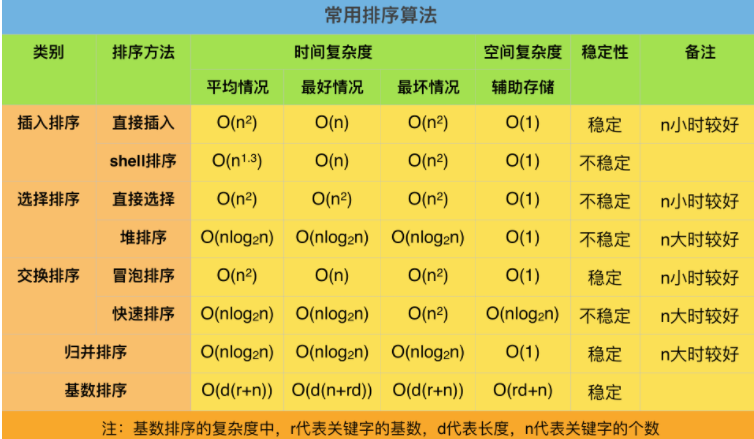
\includegraphics[width=.9\linewidth]{./pic/sort.png}

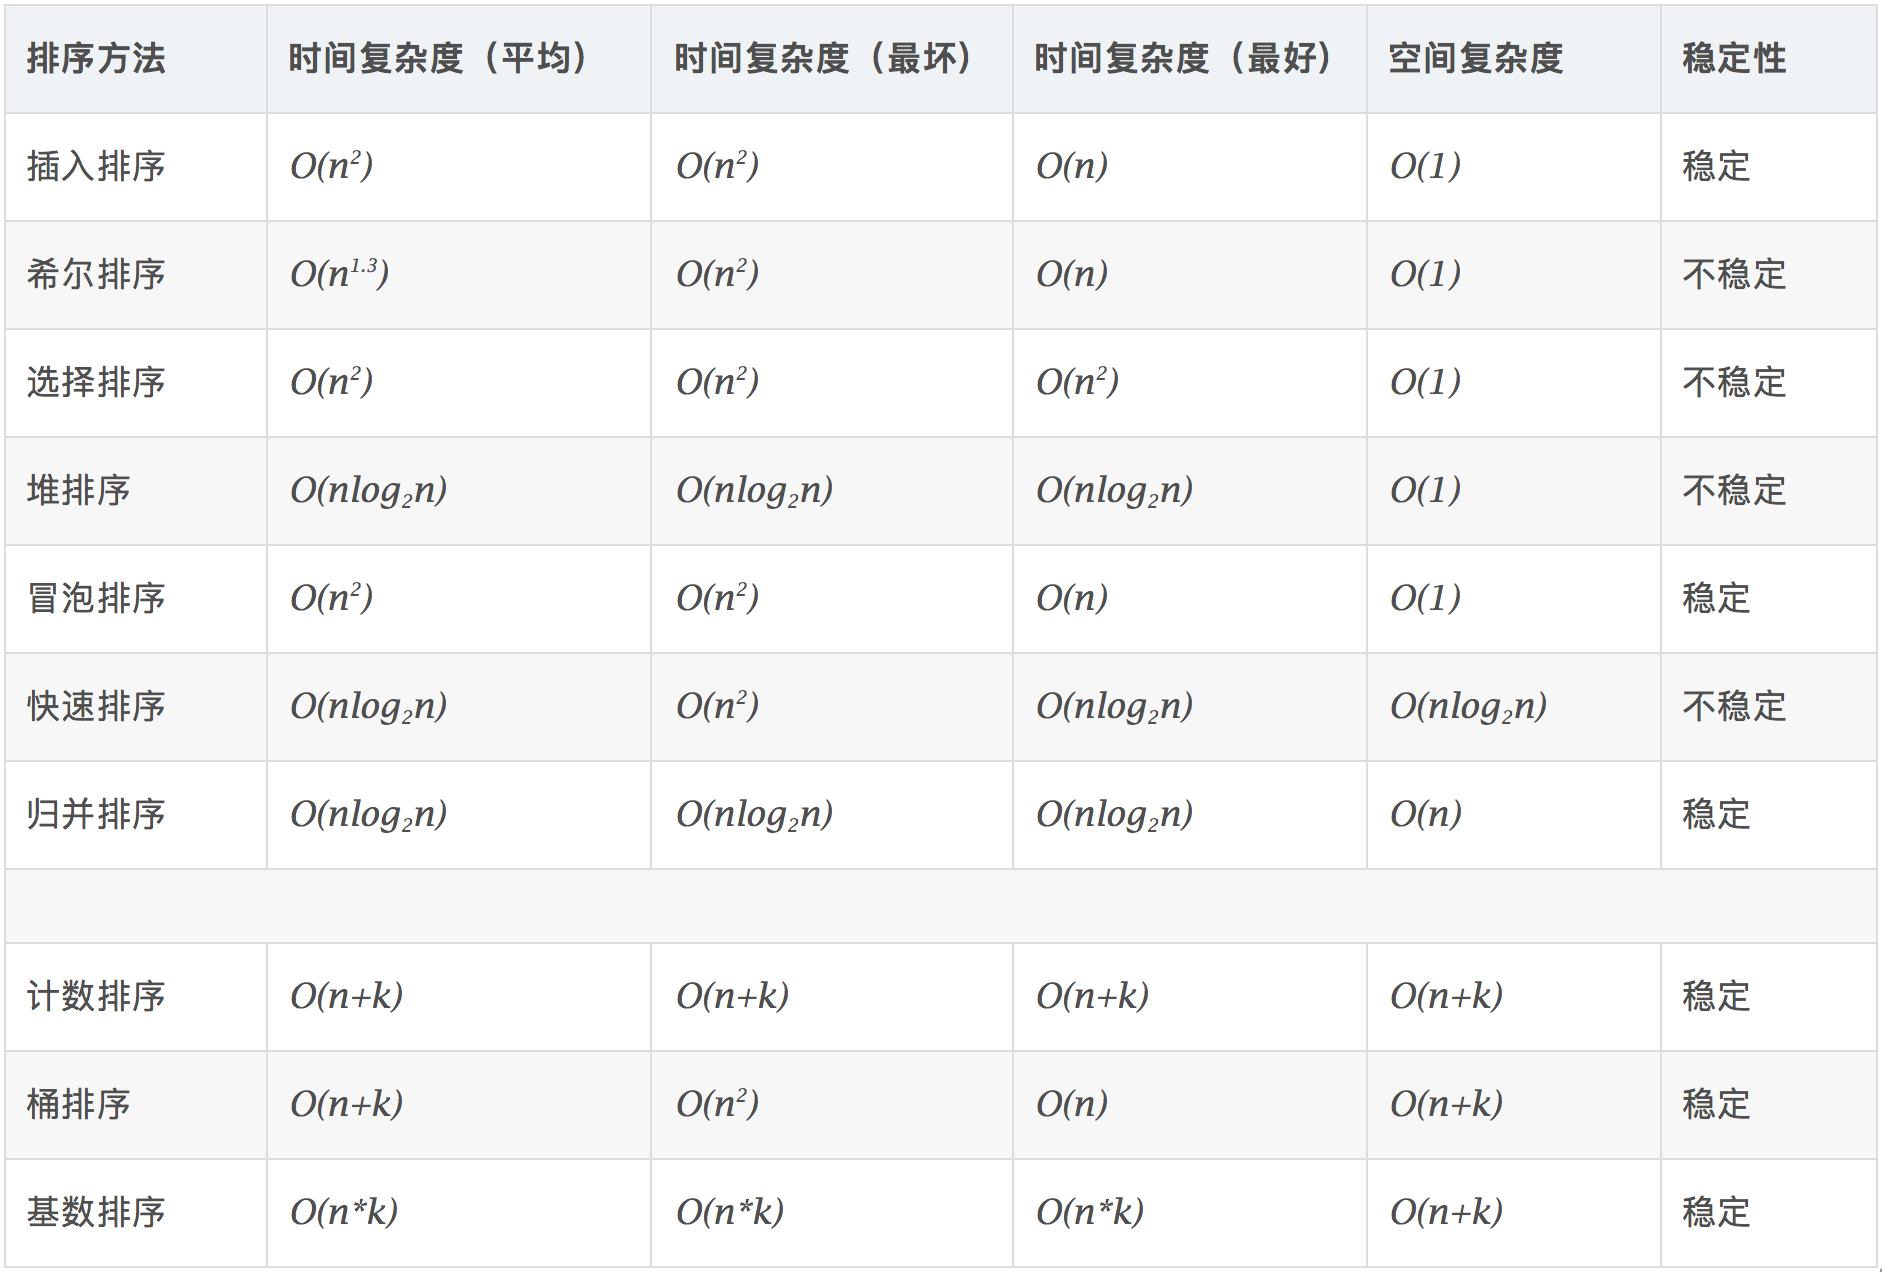
\includegraphics[width=.9\linewidth]{./pic/sort2.png}

\subsection{1996. The Number of Weak Characters in the Game 桶排序}
\label{sec-10-0-1}
You are playing a game that contains multiple characters, and each of the characters has two main properties: attack and defense. You are given a 2D integer array properties where properties[i] = [attacki, defensei] represents the properties of the ith character in the game.
A character is said to be weak if any other character has both attack and defense levels strictly greater than this character's attack and defense levels. More formally, a character i is said to be weak if there exists another character j where attackj > attacki and defensej > defensei.
Return the number of weak characters.
\begin{minted}[fontsize=\scriptsize,linenos=false]{csharp}
public int numberOfWeakCharacters(int[][] properties) {
    int maxAttrack = 0; // 找到所有士兵中的最大值
    for (int[] p : properties)
        maxAttrack = Math.max(maxAttrack,p[0]);
    // 为每一个攻击创建一个桶的位置
    int[] bucket = new int[maxAttrack + 2];     
    // 在每一个攻击力上找到最大的防御力
    for (int[] p : properties)
        bucket[p[0]] = Math.max(bucket[p[0]],p[1]);
    // 将桶的每一个位置都寻找到大于其攻击力的最大防御数值
    int rightMax = bucket[maxAttrack];
    for (int i = maxAttrack; i >= 0; i--) 
        if (rightMax > bucket[i])
            bucket[i] = rightMax;
        else
            rightMax = bucket[i];
    int ans = 0;
    // 最后遍历p 寻找所有的弱将
    for (int[] p : properties)
        if (bucket[p[0] + 1] > p[1]) ans++;  // 攻击力比当前小兵的攻击力大1的桶的位置存放着最大的防御力,与这个防御作比较可以得到当前小兵是否全面弱
    return ans;
}
public int numberOfWeakCharacters(int[][] properties) {
    int cnt = 0;
    int len = properties.length;
    Arrays.sort(properties, (a, b) -> (a[0] ! =  b[0] ? a[0]-b[0] : b[1]-a[1]));
    int max = properties[len-1][1];
    for(int i = len-1;i> = 0;i--){
        if(properties[i][1] < max)
            cnt++;
        max = Math.max(max,properties[i][1]);
    }
    return cnt;
}
\end{minted}

\subsection{Reverse Pairs}
\label{sec-10-0-2}
Given an integer array nums, return the number of reverse pairs in the array.
A reverse pair is a pair (i, j) where 0 <= i < j < nums.length and nums[i] > 2 * nums[j].
\begin{minted}[fontsize=\scriptsize,linenos=false]{csharp}
private int mergeSortCount(long [] arr, int bgn, int end) {
if (bgn >= end) return 0;
int mid = bgn + (end-bgn)/2;
int cnt = mergeSortCount(arr, bgn, mid) + mergeSortCount(arr, mid+1, end);
    for (int i = bgn, j = mid+1; i <= mid; i++) {
        while (j <= end && arr[i] > 2*arr[j]) j++;
        cnt += j - (mid+1);
    }
    Arrays.sort(arr, bgn, end+1);
    return cnt;
}
public int reversePairs(int[] nums) {
    int n = nums.length;
    return mergeSortCount(Arrays.stream(nums).mapToLong(i -> i).toArray(), 0, n-1);
}
// bit 的解法: https://www.cnblogs.com/grandyang/p/6657956.html
\end{minted}

\subsection{306. Additive Number}
\label{sec-10-0-3}
Additive number is a string whose digits can form additive sequence.

A valid additive sequence should contain at least three numbers. Except for the first two numbers, each subsequent number in the sequence must be the sum of the preceding two.

Given a string containing only digits '0'-'9', write a function to determine if it's an additive number.

Note: Numbers in the additive sequence cannot have leading zeros, so sequence 1, 2, 03 or 1, 02, 3 is invalid.
\begin{minted}[fontsize=\scriptsize,linenos=false]{csharp}
public boolean isAdditiveNumber(String num) {
    int n = num.length();
    if (n < 3) return false;
    for (int i = 1; i <= num.length() >> 1; i++)
        for (int j = 1; j + i < num.length(); j++)  
            if (isValid(num, num.substring(0, i), num.substring(i, i + j), i + j)) return true;
    return false;
}
private boolean isValid(String num, String first, String second, int index) {
    if (first.length() > 1 && first.startsWith("0") 
        || second.length() > 1 && second.startsWith("0")) return false;
    if (index == num.length()) return true; // 如果只有两个数是有效的!!!
    long sum = Long.parseLong(first) + Long.parseLong(second);
    if (num.startsWith(sum + "", index)) // 间接检测第三个数
        if (isValid(num, second, sum + "", index + (sum + "").length())) return true;
    return false;
}
\end{minted}


\chapter{Union Find 并查集}
\label{sec-11}
\subsection{1697. Checking Existence of Edge Length Limited Paths - Hard}
\label{sec-11-0-1}
An undirected graph of n nodes is defined by edgeList, where edgeList[i] = [ui, vi, disi] denotes an edge between nodes ui and vi with distance disi. Note that there may be multiple edges between two nodes.

Given an array queries, where queries[j] = [pj, qj, limitj], your task is to determine for each queries[j] whether there is a path between pj and qj such that each edge on the path has a distance strictly less than limitj .

Return a boolean array answer, where answer.length == queries.length and the jth value of answer is true if there is a path for queries[j] is true, and false otherwise.
\begin{enumerate}
\item 解题思路与分析: 离线排序优化
\label{sec-11-0-1-1}

我们可以分别对 edges 和 queries 进行一次升序排序。本题和 1170. 比较字符串最小字母出现频次 类似, 都可以采取 \textbf{离线排序优化} 的方式来解。

接下来,遍历 queries。遍历 queries 的同时将权值小于 limitj 的边进行合并。

接下来,我们只需要判断 pj 和 qj 是否已经在同一个联通域即可。

因此如果 pj 和 qj 在同一个联通域,那么其联通的路径上的所有边必定都小于 limitj,其原因就是前面加粗的那句话。

注意到排序打乱了 queries 的索引,因此我们需要记录一下其原始索引。

\begin{minted}[fontsize=\scriptsize,linenos=false]{csharp}
public boolean[] distanceLimitedPathsExist(int n, int[][] edgeList, int[][] queries) {
    DSU dsu = new DSU(n);
    Arrays.sort(edgeList, (a, b) -> a[2] - b[2]); // 同样按照weight的升序排列
    int m = queries.length, idx = 0, e = edgeList.length;
    Query [] qarr = new Query[m];
    for (int i = 0; i < m; i++) 
        qarr[i] = new Query(i, queries[i][0], queries[i][1], queries[i][2]);
    Arrays.sort(qarr);
    boolean [] ans = new boolean [m];
    for (int i = 0; i < m; i++) {
        while (idx < e && edgeList[idx][2] < qarr[i].weight) {
            dsu.union(edgeList[idx][0], edgeList[idx][1]);
            ++idx;
        }
        ans[qarr[i].idx] = dsu.areConnected(qarr[i].start, qarr[i].end);
    }            
    return ans;
}
private class DSU {
    private int N;
    private int [] parent, rank;
    public DSU( int n) {
        this.N = n;
        this.parent = new int [N];
        this.rank = new int [N];
        for (int i = 0; i < N; i++) {
            this.parent[i] = i;
            this.rank[i] = 1;
        }
    }
    public boolean areConnected(int u, int v) {
        return find(u) == find(v);
    }
    public void union(int u, int v) { // O(Log(N))
        if (u != v) {
            int p = find(u);
            int q = find(v);
            if (p != q) {
                if (rank[p] > rank[q]) {
                    parent[q] = p;
                    rank[p] += rank[q];
                } else {
                    parent[p] = q;
                    rank[q] += rank[p];
                }
            }
        }
    }
    private int find(int v) { 
        int x = v;
        while (x != parent[x])
            x = parent[x];
        parent[v] = x;
        return x;
    }
}
class Query implements Comparable<Query> {
    public int idx, start, end, weight;
    public Query(int idx, int bgn, int end, int weight) {
        this.idx = idx;
        this.start = bgn;
        this.end = end;
        this.weight = weight;
    }
    @Override public int compareTo(Query query) { // 按照weight的升序排列
        return this.weight - query.weight;
    }
}
// 令 m, q edges 和 queries 的长度。
//     时间复杂度:$O(mlogm + qlogq)
//     空间复杂度:$O(n + q)
// Runtime is bound by sorting: O(ElogE + NlogN + N + E);
\end{minted}
\end{enumerate}

\subsection{2003. Smallest Missing Genetic Value in Each Subtree - Hard}
\label{sec-11-0-2}
There is a family tree rooted at 0 consisting of n nodes numbered 0 to n - 1. You are given a 0-indexed integer array parents, where parents[i] is the parent for node i. Since node 0 is the root, parents\footnotemark[1]{} == -1.

There are 105 genetic values, each represented by an integer in the inclusive range [1, 105]. You are given a 0-indexed integer array nums, where nums[i] is a distinct genetic value for node i.

Return an array ans of length n where ans[i] is the smallest genetic value that is missing from the subtree rooted at node i.

The subtree rooted at a node x contains node x and all of its descendant nodes.
\begin{minted}[fontsize=\scriptsize,linenos=false]{csharp}
private void dfs(int i, Set<Integer> visited, int [] arr) { // 图的遍历:自顶向下ok,自底向上还不太熟悉,需要练习,还有一个没有消化好的类似题,找出来binary indexed tree
    if (!visited.contains(arr[i])) {
        Set<Integer> children = tree.getOrDefault(i, new HashSet<Integer>());
        for (int v : children) 
            dfs(v, visited, arr);
        visited.add(arr[i]);
    }
}
Map<Integer, Set<Integer>> tree = new HashMap<>();
int [] ans;
int n;
public int[] smallestMissingValueSubtree(int[] parents, int[] nums) {
    n = parents.length;
    ans = new int [n];
    Arrays.fill(ans, 1); 
    int oneIdx = -1;
    for (int i = 0; i < n; i++) 
        if (nums[i] == 1) {
            oneIdx = i;
            break;
        }
    if (oneIdx == -1) return ans;
    for (int i = 1; i < n; i++) {
        tree.computeIfAbsent(parents[i], k -> new HashSet<Integer>());
        tree.get(parents[i]).add(i);
        // tree.computeIfAbsent(i, k -> new HashSet<Integer>()); // 这里要想一下:为什么双向图他只加一个方向?
        // tree.get(i).add(parents[i]);
    }
    Set<Integer> visited = new HashSet<>(); // 这个直接转化为想要的结果,很便捷
    int parentIter = oneIdx;
    int miss = 1;
    while (parentIter >= 0) { // 从值为1的节点向根遍历(自底向上),没有任何重复计算,只走完这一条自底向项的路径就可以了
        dfs(parentIter, visited, nums);
        while (visited.contains(miss)) ++miss;
        ans[parentIter] = miss;
        parentIter = parents[parentIter];
    }
    return ans;
}
\end{minted}

\subsection{803. Bricks Falling When Hit - Hard 反向: 变de-Union vs为 Re-Union}
\label{sec-11-0-3}
You are given an m x n binary grid, where each 1 represents a brick and 0 represents an empty space. A brick is stable if:

It is directly connected to the top of the grid, or
At least one other brick in its four adjacent cells is stable.
You are also given an array hits, which is a sequence of erasures we want to apply. Each time we want to erase the brick at the location hits[i] = (rowi, coli). The brick on that location (if it exists) will disappear. Some other bricks may no longer be stable because of that erasure and will fall. Once a brick falls, it is immediately erased from the grid (i.e., it does not land on other stable bricks).

Return an array result, where each result[i] is the number of bricks that will fall after the ith erasure is applied.

Note that an erasure may refer to a location with no brick, and if it does, no bricks drop.


\includegraphics[width=.9\linewidth]{./pic/hitBricks.png}

\begin{minted}[fontsize=\scriptsize,linenos=false]{csharp}
private class UnionFind {
    int [] id; // parent
    int [] cnt;// size
    public UnionFind (int n) {
        id = new int [n];
        cnt = new int [n];
        for (int i = 0; i < n; i++) {
            id[i] = i;
            cnt[i] = 1;
        }
    }
    public int find(int i) {
        while (id[i] != i) {
            id[i] = id[id[i]];
            i = id[i];
        }
        return i;
    }
    public void union(int i, int j) {
        int rootI = find(i);
        int rootJ = find(j);
        if (rootI != rootJ) {
            id[rootI] = rootJ;
            cnt[rootJ] += cnt[rootI];
        }
    }
}
private void unionAround(int x, int y, int [][] arr, UnionFind uf) {
    for (int [] d : dirs) {
        int i = x + d[0];
        int j = y + d[1];
        if (i < 0 || i >= m || j < 0 || j >= n) continue;
        if (arr[i][j] == 1) uf.union(x*n+y+1, i*n+j+1); // +1
    }
    if (x == 0) uf.union(x*n+y+1, 0); // 第一排的直接与顶相连 // trick: to help calculate cnts connecting top easier/faster
}
int [][] dirs = {{1, 0}, {-1, 0}, {0, 1}, {0, -1}};
int m, n;
public int[] hitBricks(int[][] grid, int[][] hits) {
    m = grid.length;
    n = grid[0].length;
    for (int [] hit : hits)              // 首先把所有要打的砖块标记为2.
        if (grid[hit[0]][hit[1]] == 1)   // 如果有砖头
            grid[hit[0]][hit[1]] = 2;
    UnionFind uf = new UnionFind(m*n+1); // 这里的 + 1主要是多一个0来表示顶,所有的第一排的砖在unionfind的时候都会直接与这个0相连。
    for (int i = 0; i < m; i++)          // 然后对打掉后的数组中的砖块进行四个方向的union
        for (int j = 0; j < n; j++) 
            if (grid[i][j] == 1)
                unionAround(i, j, grid, uf);
    int cnt = uf.cnt[uf.find(0)];        // 这个count就是打完后一定会剩下的砖块数量.
    int [] ans = new int [hits.length];
    for (int i = hits.length-1; i >= 0; i--) {
        int [] hit = hits[i];
        if (grid[hit[0]][hit[1]] == 2) { // 对于需要复原的这个砖块做四个方向union,主要是为了得到有多少砖必须通过这块砖才能连接到顶部。
            unionAround(hit[0], hit[1], grid, uf);
            grid[hit[0]][hit[1]] = 1;    // 由于是从后向前,做完要把这块砖重新标记回来: 这些砖是有可能被hits前序砖敲掉后掉落下来的,不复原影响前序结果
        }
        int newCnt = uf.cnt[uf.find(0)];
        ans[i] = (newCnt - cnt > 0 ? newCnt - cnt - 1 : 0);
        cnt = newCnt;
    }
    return ans;
}
\end{minted}

\subsection{721. Accounts Merge}
\label{sec-11-0-4}
Given a list of accounts where each element accounts[i] is a list of strings, where the first element accounts[i]\footnotemark[1]{} is a name, and the rest of the elements are emails representing emails of the account.

Now, we would like to merge these accounts. Two accounts definitely belong to the same person if there is some common email to both accounts. Note that even if two accounts have the same name, they may belong to different people as people could have the same name. A person can have any number of accounts initially, but all of their accounts definitely have the same name.

After merging the accounts, return the accounts in the following format: the first element of each account is the name, and the rest of the elements are emails in sorted order. The accounts themselves can be returned in any order.

\begin{itemize}
\item Similar to the most voted solution, my solution uses the index of the owner as the key for the union map, to avoid possible issue caused by different owners have the same name, thus uses one less loop.
\end{itemize}

\begin{minted}[fontsize=\scriptsize,linenos=false]{csharp}
private int findParent(int [] arr, int x) {
    if (arr[x] == x) return x;
    arr[x] = findParent(arr, arr[x]);
    return arr[x];
}
public List<List<String>> accountsMerge(List<List<String>> accounts) {
    Map<String, Integer> owner = new HashMap<>();
    Map<Integer, TreeSet<String>> union = new HashMap<>(); // match idx & Set<Sting emails>
    int n = accounts.size(), p = 0;
    int [] par = new int [n];
    for (int i = 0; i < n; i++) par[i] = i;
    List<String> ls = new ArrayList<>(); 
    for (int i = 0; i < n; i++) { // find the ownerIdx for each email address
        ls = accounts.get(i);
        for (int j = 1; j < ls.size(); j++) {
            String email = ls.get(j);
            if (owner.containsKey(email)) {
                p = findParent(par, owner.get(email));
                par[p] = i; // union accounts that belong to the same user here by updating parent relation
            }
            owner.put(email, i);
        }
    }
     // union all emails belong to the same owner
    for (String emal : owner.keySet()) {
        int ownerIdx = findParent(par, owner.get(emal));
        TreeSet<String> set = union.getOrDefault(ownerIdx, new TreeSet<>());
        set.add(emal);
        union.put(ownerIdx, set);
    }
// Generate return result
    List<List<String>> res = new ArrayList<>();
    for (int ownerIdx : union.keySet()) {
        ls = new ArrayList<>();
        ls.add(accounts.get(ownerIdx).get(0));  // get the owner name
        ls.addAll(union.get(ownerIdx));
        res.add(ls);
    }
    return res;
}
\end{minted}

\subsection{1202. Smallest String With Swaps}
\label{sec-11-0-5}
You are given a string s, and an array of pairs of indices in the string pairs where pairs[i] = [a, b] indicates 2 indices(0-indexed) of the string.

You can swap the characters at any pair of indices in the given pairs any number of times.

Return the lexicographically smallest string that s can be changed to after using the swaps.
\begin{minted}[fontsize=\scriptsize,linenos=false]{csharp}
int [] par;
int [] rank;
int n;
public int find(int v) {
    if (v != par[v] ) 
        par[v] = find(par[v]);
    return par[v];
}
public boolean union(int i, int j) {
    int ri = find(i);
    int rj = find(j);
    if (ri == rj) return false;
    if (rank[ri] < rank[rj]) par[ri] = rj;
    else if (rank[ri] > rank[rj]) par[rj] = ri;
    else {
        par[rj] = ri;
        rank[ri] ++; // 维护rank的值
    }
    return true;
}
public String smallestStringWithSwaps(String s, List<List<Integer>> pairs) {
    int n = s.length();
    par = new int [n];
    rank = new int [n];
    List<Queue<Character>> list = new ArrayList<>(n);
    for (int i = 0; i < n; i++) {
        par[i] = i;
        list.add(new PriorityQueue<>());
    }
    Arrays.fill(rank, 1);
    pairs.forEach(p -> union(p.get(0), p.get(1))); // Perform union for each pair.
    // Add each character to the priority queue associated with its component.
    IntStream.range(0, n).forEach(index -> list.get(find(index)).add(s.charAt(index)));
    // Build the result, by removing chars from the corresponding priority queue.
    StringBuilder buffer = new StringBuilder(n);
    IntStream.range(0, n).forEachOrdered(index -> buffer.append(list.get(find(index)).remove()));
    return buffer.toString();
}
// O(NlogN). Worst-case, all indices are part of the same component. So we will essentially be popping off from the same priority queue.
// Space Complexity: O(N).
\end{minted}

\subsection{1998. GCD Sort of an Array - Hard}
\label{sec-11-0-6}
You are given an integer array nums, and you can perform the following operation any number of times on nums:

Swap the positions of two elements nums[i] and nums[j] if gcd(nums[i], nums[j]) > 1 where gcd(nums[i], nums[j]) is the greatest common divisor of nums[i] and nums[j].
Return true if it is possible to sort nums in non-decreasing order using the above swap method, or false otherwise.
\begin{minted}[fontsize=\scriptsize,linenos=false]{csharp}
private int find (int v) {
    if (!parent.containsKey(v)) {
        parent.put(v, v);
        return v;
    }
    if (parent.get(v) != v)
        parent.put(v, find(parent.get(v)));
    return parent.get(v);
}
private void union(int x, int y) {
    int rx = find(x);
    int ry = find(y);
    if (rx != ry) parent.put(rx, ry);
}
/**
   general idea (not accepted)
   we can simply union pairs of numbers which has gcd > 1 in quadratic time and then check of groups that
   are formed by union of pairs can be invidually sorted. 
   improved (accpeted)
   In above approach problem is we are union-ing pairs in quadratic time. To improve upon it. We union a number
   which is present in 'nums' with its smallest prime factor. thus if two numbers has same smallest prime factor
   their gcd is guaranted to be > 1. 
**/
Map<Integer, Integer> parent = new HashMap<>();
public boolean gcdSort(int[] arr) {
    int n = arr.length;
    parent = new HashMap<Integer, Integer>();
    int [] sorted = arr.clone();
    Arrays.sort(sorted);
    int max = Arrays.stream(arr).max().getAsInt();
    Set<Integer> numSet = new HashSet<>();
    numSet.addAll(Arrays.stream(arr).boxed().collect(Collectors.toList()));
    int p = 2;  // Seive algorithm
    boolean [] primes = new boolean [max + 1];
    Arrays.fill(primes, true);
    while (p < max) {
        if (primes[p]) {
            for (int i = p; i <= max; i += p) { // 我合并的是数组的索引,他优化成合并所有拥有公约数为p的数组中沿未合并的值
                if (numSet.contains(i)) union(p, i);
                primes[i] = false;
            }
        }
        p++;
    }
    for (int i = 0; i < n; i++) 
        if (arr[i] != sorted[i] && find(sorted[i]) != find(arr[i])) return false;
    return true;
}
\end{minted}

\subsection{1724 给定一个n nn个顶点的无向带权图,要求在线回答若干询问,每次询问是个三元组( p , q , x ) (p,q,x)(p,q,x),是问是否存在p pp到q qq的每条边都小于x xx的路径。}
\label{sec-11-0-7}

先以Kruskal算法求最小生成森林,显然对于任何p pp和q qq,它们之间所有路径中最大边最小的那条路径的最大边一定是最小生成树的某条边(如果存在路径的话)。建树完成之后,对每个连通块,以任意顶点为根,将该连通块做成一棵有根树。对于每次询问,我们只需求p pp和q qq所有到它们的最近公共祖先所经过的边的最大边权就行了。可以考虑用倍增思想(以下的内容可以参考\url{https://blog.csdn.net/qq_46105170/article/details/116217633),开两个数组f} ff和g gg,其中f [ i ] [ k ] f[i][k]f[i][k]指的是从i ii节点向上跳2 k 2\^{}k2 
k
 步能过走到的顶点是谁(如果跳出界了则规定值为− 1 -1−1),g [ i ] [ k ] g[i][k]g[i][k]指的是从i ii节点向上跳2 k 2\^{}k2 
k
 的过程中经过的边的最大权值(在不会跳出界的情况下),然后从每个树根做BFS,初始化f [ . ] [ 0 ] f[.]\footnotemark[1]{}f[.]\footnotemark[1]{}和g [ . ] [ 0 ] g[.]\footnotemark[1]{}g[.]\footnotemark[1]{}。由于在询问的时候需要知道最近公共祖先,所以还需要一个数组d dd记录每个顶点的深度,在BFS的时候可以同时求出。接下来,用倍增的思想计算f ff和g gg:
\begin{minted}[fontsize=\scriptsize,linenos=false]{csharp}
f[i][k] = f[f[i][k-1]][k-1]
g[i][k] = max{g[i][k-1],g[f[i][k-1]][k-1]}
\end{minted}
至此,所有的预处理就完成了。

接下来询问的时候,如果p pp与q qq不连通则直接返回false。否则看一下两个顶点的深度,不妨设p pp更深,则将p pp向上跳若干步,使得p pp与q qq一样深,同时用经过的边权更新答案。此时如果p = q p=qp=q,则答案已经求出,与x xx比较即可;否则,将p pp与q qq继续向上跳,一路跳到它们的最近公共祖先的孩子的那层位置,一路更新答案,最后再用最近公共祖先与它们的连边更新答案,最后将答案与x xx比较。代码如下:
\begin{minted}[fontsize=\scriptsize,linenos=false]{csharp}
public class DistanceLimitedPathsExist {
    class UnionFind {
        private int[] p;
        public UnionFind(int size) {
            p = new int[size];
            for (int i = 0; i < size; i++) 
                p[i] = i;
        }
        public int find(int x) {
            if (p[x] != x) 
                p[x] = find(p[x]);
            return p[x];
        }
        public void union(int x, int y) {
            int px = find(x), py = find(y);
            if (px != py) 
                p[px] = py;
        }
    }
    private UnionFind uf;
    // 这里是链式前向星建图
    private int[] h, e, ne, w;
    private int idx;
    private void add(int a, int b, int c) {
        e[idx] = b;
        ne[idx] = h[a];
        w[idx] = c;
        h[a] = idx++;
    }
    // 这里是倍增法所需的数组和变量
    private int[][] f, g;
    private int[] depth;
    // n是顶点数,log是n对2的对数,log + 1也是f的第二维应该开的长度
    private int n, log;
    public DistanceLimitedPathsExist(int n, int[][] edgeList) {
        this.n = n;
        depth = new int[n];
        h = new int[n];
        Arrays.fill(h, -1);
        // 无向图,边要开两倍
        e = new int[n << 1];
        ne = new int[n << 1];
        w = new int[n << 1];
        // 这一段是Kruskal算法建最小生成森林
        Arrays.sort(edgeList, (e1, e2) -> Integer.compare(e1[2], e2[2]));
        uf = new UnionFind(n);
        for (int[] e : edgeList) {
            int a = e[0], b = e[1], len = e[2];
            if (uf.find(a) != uf.find(b)) {
                uf.union(a, b);
                add(a, b, len);
                add(b, a, len);
            }
        }
        log = (int) (Math.log(n) / Math.log(2));
        f = new int[n][log + 1];
        g = new int[n][log + 1];
        for (int[] row : f) {
            Arrays.fill(row, -1);
        }
        boolean[] vis = new boolean[n];
        for (int i = 0; i < n; i++) {
            if (!vis[i]) {
                bfs(i, vis);
            }
        }
        init();
    }
    // 递推一遍f和g数组
    private void init() {
        for (int i = 1; i < log + 1; i++) {
            for (int j = 0; j < n; j++) {
                if (f[j][i - 1] != -1) {
                    f[j][i] = f[f[j][i - 1]][i - 1];
                    g[j][i] = Math.max(g[j][i - 1], g[f[j][i - 1]][i - 1]);
                }
            }
        }
    }
    // BFS一遍x所在连通块,并初始化f和g数组,并求出depth数组
    private void bfs(int x, boolean[] vis) {
        Queue<Integer> q = new ArrayDeque<>();
        q.offer(x);
        vis[x] = true;
        while (!q.isEmpty()) {
            int u = q.poll();
            for (int i = h[u]; i != -1; i = ne[i]) {
                int v = e[i];
                if (vis[v]) continue;
                vis[v] = true;
                f[v][0] = u;
                g[v][0] = w[i];
                q.offer(v);
                depth[v] = depth[u] + 1;
            }
        }
    }
    public boolean query(int p, int q, int limit) {
        if (uf.find(p) != uf.find(q)) 
            return false;
        if (depth[p] < depth[q]) {
            int tmp = p;
            p = q;
            q = tmp;
        }
        // 先走到同一深度
        int diff = depth[p] - depth[q];
        int pow = 0, max = 0;
        while (diff > 0) {
            if ((diff & 1) == 1) {
                max = Math.max(max, g[p][pow]);
                p = f[p][pow];
            }

            pow++;
            diff >>= 1;
        }
        // 已经走到同一点了,那深度更浅的那个点就是最近公共祖先,max就是经过的边的最大值
        if (p == q) return max < limit;
        // 否则跳到最近公共祖先下面一层,沿途更新答案
        for (int i = log; i >= 0; i--) {
            if (f[p][i] != f[q][i]) {
                max = Math.max(max, g[p][i]);
                max = Math.max(max, g[q][i]);
                p = f[p][i];
                q = f[q][i];
            }
        }
        // 最后别忘了用最后一步更新答案
        max = Math.max(max, g[p][0]);
        max = Math.max(max, g[q][0]);
        return max < limit;
    }
}
// 初始化时间复杂度O ( m log ⁡ m + n log ⁡ n ) O(m\log m+n\log n)O(mlogm+nlogn),每次询问时间O ( log ⁡ n ) O(\log n)O(logn),空间O ( m + n + n log ⁡ n ) O(m+n+n\log n)O(m+n+nlogn)。
\end{minted}

\subsection{1172. 祖孙询问}
\label{sec-11-0-8}
给定一棵包含n nn个节点的有根无向树,节点编号互不相同,但不一定是1 ∼ n 1∼n1∼n。有m mm个询问,每个询问给出了一对节点的编号x xx和y yy,询问x xx与y yy的祖孙关系。

输入格式:
输入第一行包括一个整数 表示节点个数;接下来n nn行每行一对整数a aa和b bb,表示a aa和b bb之间有一条无向边。如果b bb是− 1 −1−1,那么a aa就是树的根;第n + 2 n+2n+2行是一个整数m mm表示询问个数;接下来m mm行,每行两个不同的正整数x xx和y yy,表示一个询问。

输出格式:
对于每一个询问,若x xx是y yy的祖先则输出1 11,若y yy是x xx的祖先则输出2 22,否则输出0 00。

数据范围:
1 ≤ n , m ≤ 4 × 1 0 4 1≤n,m≤4×10\^{}41≤n,m≤4×10 
4

1 ≤ v ≤ 4 × 1 0 4 1≤v≤4×10\^{}41≤v≤4×10 
4
 ,v vv是顶点编号

可以用倍增的思想来求。预处理两个数组,一个是d [ i ] d[i]d[i],指的是顶点i ii的深度,树根深度是1 11,其余顶点的深度就是其与树根的路径边数;另一个是f [ i ] [ k ] f[i][k]f[i][k],是从顶点i ii向树根方向(以下均称“向上”)跳2 k 2\^{}k2 
k
 步走到的顶点。由于顶点编号都是大于0 00的,我们可以人为规定一个0 00号节点作为哨兵,并且∀ k , f [ r ] [ k ] = 0 $\forall$ k,f[r][k]=0∀k,f[r][k]=0,d [ 0 ] = 0 d\footnotemark[1]{}=0d\footnotemark[1]{}=0,其中r rr是树根编号。这样如果k kk太大导致跳出树根的话,就会得到跳到了哨兵的结论。那么对于f ff,有f [ i ] [ 0 ] = p i f[i]\footnotemark[1]{}=p\_if[i]$\backslash$footnotemark[1]\{\}= 是i ii的父亲,并且:

f[i][k]=f[f[i][k−1]][k−1]

即分两次跳,一次跳2\^{}k 步等价于两次跳2\^{}k-1 步。初始化f ff和d dd数组的过程,可以用一次从树根的BFS来做到。

在询问的时候,比如询问a aa和b bb的公共祖先,不妨设a aa的深度更深,那么先让a aa向上跳到与b bb深度相同,可以先计算一下d [ a ] − d [ b ] d[a]-d[b]d[a]−d[b],然后将这个数字做二进制分解,就可以由f ff数组算出从a aa向上走到与b bb深度相同的时候是哪个顶点;接着再从a aa和b bb一起向上走,直到走到它们真正的最近公共祖先的下一层为止(即跳的步数是当前深度差减1 11),此时f [ a ] [ 0 ] f[a]\footnotemark[1]{}f[a]\footnotemark[1]{}即为最近公共祖先。代码如下:
\begin{minted}[fontsize=\scriptsize,linenos=false]{c++}
const int N = 40010, M = N * 2;
int n, m;
int h[N], e[M], ne[M], idx;
int depth[N], fa[N][16];
int q[N];
void add(int a, int b) {
    e[idx] = b, ne[idx] = h[a], h[a] = idx++;
}
// 从树根开始bfs,预处理出d数组和f数组
void bfs(int root) {
    memset(depth, 0x3f, sizeof depth);
    depth[0] = 0, depth[root] = 1;
    int hh = 0, tt = 0;
    q[tt++] = root;
    while (hh < tt) {
        int t = q[hh++];
        for (int i = h[t]; ~i; i = ne[i]) {
            int j = e[i];
            if (depth[j] > depth[t] + 1) {
                depth[j] = depth[t] + 1;
                q[tt++] = j;
                // 预处理f数组
                fa[j][0] = t;
                for (int k = 1; k <= 15; k++) 
                    fa[j][k] = fa[fa[j][k - 1]][k - 1];
            }
        }
    }
}
int lca(int a, int b) {
	// 强制让a的深度大于等于b的深度
    if (depth[a] < depth[b]) swap(a, b);
    // 从大到小枚举k,将a向上跳到与b同层
    for (int k = 15; k >= 0; k--)
        if (depth[fa[a][k]] >= depth[b]) 
            a = fa[a][k];
	// 如果a和b重合了,那么说明b就是最近公共祖先
    if (a == b) return b;
    // 否则将a和b同时向上跳,直到跳到最近公共祖先下一层为止
    for (int k = 15; k >= 0; k--)
        if (fa[a][k] != fa[b][k])
            a = fa[a][k], b = fa[b][k];
    return fa[a][0];
}
int main() {
    scanf("%d", &n);
    memset(h, -1, sizeof h);
    int root = 0;
    for (int i = 0; i < n; i++) {
        int a, b;
        scanf("%d%d", &a, &b);
        if (b == -1) root = a;
        else add(a, b), add(b, a);
    }
    bfs(root);
    scanf("%d", &m);
    while (m--) {
        int a, b;
        scanf("%d%d", &a, &b);
        int p = lca(a, b);
        if (p == a) puts("1");
        else if (p == b) puts("2");
        else puts("0");
    }
    return 0;
}
\end{minted}

\subsection{某个网友列的相关题目: 并查集参考:数据结构–并查集(Disjoint-Set)}
\label{sec-11-0-9}
\begin{itemize}
\item 261. 以图判树(全部连通+边数=V-1)
\item 305. 岛屿数量 II(并查集)
\item 323. 无向图中连通分量的数目(并查集)
\item 684. 冗余连接(并查集)
\item 685. 冗余连接 II(并查集)
\item 721. 账户合并(并查集)(字符串合并)
\item 737. 句子相似性 II(并查集)
\item 886. 可能的二分法(着色DFS/BFS/拓展并查集)
\item 947. 移除最多的同行或同列石头(并查集)
\item 990. 等式方程的可满足性(并查集)
\item 959. 由斜杠划分区域(并查集)
\item 1061. 按字典序排列最小的等效字符串(并查集)
\item 1101. 彼此熟识的最早时间(排序+并查集)
\item 1202. 交换字符串中的元素(并查集)
\item 1319. 连通网络的操作次数(BFS/DFS/并查集)
\item 5510. 保证图可完全遍历(并查集)
\item 程序员面试金典 - 面试题 17.07. 婴儿名字(并查集)
\end{itemize}

\chapter{Graph}
\label{sec-12}
\section{拓扑排序}
\label{sec-12-1}
\subsection{1857. Largest Color Value in a Directed Graph - Hard}
\label{sec-12-1-1}
There is a directed graph of n colored nodes and m edges. The nodes are numbered from 0 to n - 1.

You are given a string colors where colors[i] is a lowercase English letter representing the color of the ith node in this graph (0-indexed). You are also given a 2D array edges where edges[j] = [aj, bj] indicates that there is a directed edge from node aj to node bj.

A valid path in the graph is a sequence of nodes x1 -> x2 -> x3 -> \ldots{} -> xk such that there is a directed edge from xi to xi+1 for every 1 <= i < k. The color value of the path is the number of nodes that are colored the most frequently occurring color along that path.

Return the largest color value of any valid path in the given graph,
or -1 if the graph contains a cycle.
\begin{enumerate}
\item 解题思路与分析
\label{sec-12-1-1-1}
\begin{minted}[fontsize=\scriptsize,linenos=false]{csharp}
public int largestPathValue(String colors, int[][] edges) {
    List<List<Integer>> adj = new ArrayList<>();
    int n = colors.length(), cnt = 0; 
    int [] ins = new int [n], topo = new int [n]; 
    for (int i = 0; i < n; i++) adj.add(new ArrayList<>());
    for (int [] e : edges) {
        ins[e[1]]++;
        adj.get(e[0]).add(e[1]);
    }
    Queue<Integer> q = new LinkedList<>();
    for (int i = 0; i < n; i++)
        if (ins[i] == 0)
            q.offer(i);
    while (!q.isEmpty()) {
        int u = q.poll();
        topo[cnt++] = u; // 将所有的节点按照拓扑排序
        for (Integer v : adj.get(u)) 
            if (--ins[v] == 0)
                q.offer(v);
    }
    if (cnt < n) return -1; // 说明图中有环
    int ans = 0;
    char [] s = colors.toCharArray();
    for (int i = 0; i < 26; i++) {
        char c = (char)(i + 'a');
        int [] dp = new int [n];
        for (int j = n-1; j >= 0; j--) {
            int u = topo[j];
            for (Integer v : adj.get(u)) 
                dp[u] = Math.max(dp[u], dp[v]);
            if (s[u] == c) dp[u]++;
            ans = Math.max(ans, dp[u]);
        }
    }
    return ans;
}
\end{minted}
\begin{itemize}
\item 另一种更为简洁的写法
\end{itemize}
\begin{minted}[fontsize=\scriptsize,linenos=false]{csharp}
public int largestPathValue(String colors, int[][] edges) {
    int n = colors.length(), ans = 0, processed = 0;
    int[] ins = new int[n];
    ArrayList<Integer> [] adj = new ArrayList[n];
    Queue<Integer> q = new LinkedList<>();
    int[][] cnt = new int[n][26];
    for (int i = 0; i < n; ++i) adj[i] = new ArrayList<>();
    for (int [] e : edges) {
        adj[e[0]].add(e[1]);
        ++ins[e[1]];
    }
    for (int i = 0; i < n; ++i)
        if (ins[i] == 0)
            q.offer(i);
    char [] s = colors.toCharArray();
    while (!q.isEmpty()) {
        int u = q.poll();
        ++processed;
        ans = Math.max(ans, ++cnt[u][s[u] - 'a']);
        for (int v : adj[u]) {
            for (int i = 0; i < 26; ++i)
                cnt[v][i] = Math.max(cnt[v][i], cnt[u][i]); // 这里是不是可以再简化一下?
            if (--ins[v] == 0)
                q.offer(v);
        }
    }
    return processed == n ? ans : -1;
}
\end{minted}
\end{enumerate}
\subsection{1203. Sort Items by Groups Respecting Dependencies - Hard}
\label{sec-12-1-2}
There are n items each belonging to zero or one of m groups where group[i] is the group that the i-th item belongs to and it's equal to -1 if the i-th item belongs to no group. The items and the groups are zero indexed. A group can have no item belonging to it.

Return a sorted list of the items such that:

The items that belong to the same group are next to each other in the sorted list.
There are some relations between these items where beforeItems[i] is a list containing all the items that should come before the i-th item in the sorted array (to the left of the i-th item).
Return any solution if there is more than one solution and return an empty list if there is no solution.
\begin{enumerate}
\item 解题思路与分析
\label{sec-12-1-2-1}
\begin{minted}[fontsize=\scriptsize,linenos=false]{csharp}
public int[] sortItems(int n, int m, int[] g, List<List<Integer>> bef) {
    List<List<Integer>> its = new ArrayList<>(); // 下标:元素所属的组编号;组内元素
    List<List<Integer>> gps = new ArrayList<>(); // 组图: 下标: 组编号;组内元素
    List<Integer> ids = new ArrayList<>();
    for (int i = 0; i < m+n; i++) {
        ids.add(i);
        its.add(new ArrayList<>());
        gps.add(new ArrayList<>());
    }
    List<List<Integer>> itg = new ArrayList<>(); // itemGraph, n items, 元素先后順序图:每个元素,之后的元素包括()
    for (int i = 0; i < n; i++) 
        itg.add(new ArrayList<>());
    int [] insIts = new int [n];   // 每个元素各自入度
    int [] insGps = new int [m+n]; // 每个组的各自入度
    int resId = m; // 把先前剩余的、不属于任何组的,分别分布到只含其一个元素的编号较大(编号不被其它元素占用[0, m-1])的组中
    for (int i = 0; i < n; i++) {
        if (g[i] == -1)
            g[i] = resId++;
        its.get(g[i]).add(i); // 下标:元素所属的组编号;组内元素
    }
    for (int i = 0; i < n; i++) {
        int gid = g[i];
        for (int it : bef.get(i)) { // 在现元素i之前的元素链表
            int befGid = g[it];
            if (befGid == gid) { // 在同一个组内,可以进行组内排序
                insIts[i]++;
                itg.get(it).add(i);       // 从之前的元素可以连接到现元素 <== 会进行拓扑排序,所有先发生的在前,后发生的在后
            } else {             // 属于不同的组,须进行组间排序
                if (gps.get(gid).contains(befGid)) return new int [0]; // 这里发生了矛盾,需返回
                insGps[gid]++;
                gps.get(befGid).add(gid); // 从之前的组可以连接到现组     <== 会进行拓扑排序,所有先发生的在前,后发生的在后
            }
        }
    }
    List<Integer> gsort = topologicalSort(insGps, gps, ids); // 组间排序
    if (gsort.size() == 0) return new int [0];
    int [] ans = new int [n];
    int i = 0;
    for (Integer gid : gsort) { // 对排好序的各组,进行组内排序
        int size = its.get(gid).size();
        if (size == 0) continue;
        List<Integer> li = topologicalSort(insIts, itg, its.get(gid)); // 进行组内排序
        if (li.size() == 0) return new int [0];
        for (int it : li) 
            ans[i++] = it;
    }
    return ans;
}
List<Integer> topologicalSort(int [] ins, List<List<Integer>> adj, List<Integer> li) {
    Deque<Integer> q = new ArrayDeque<>();
    for (Integer v : li) 
        if (ins[v] == 0) q.offerLast(v);
    List<Integer> ans = new ArrayList<>();
    while (!q.isEmpty()) {
        int cur = q.pollFirst();
        ans.add(cur);
        for (Integer v : adj.get(cur)) 
            if (--ins[v] == 0) q.offerLast(v);
    }
    return ans;
}
\end{minted}
\end{enumerate}
\subsection{2045. Second Minimum Time to Reach Destination - Hard}
\label{sec-12-1-3}
A city is represented as a bi-directional connected graph with n vertices where each vertex is labeled from 1 to n (inclusive). The edges in the graph are represented as a 2D integer array edges, where each edges[i] = [ui, vi] denotes a bi-directional edge between vertex ui and vertex vi. Every vertex pair is connected by at most one edge, and no vertex has an edge to itself. The time taken to traverse any edge is time minutes.

Each vertex has a traffic signal which changes its color from green to red and vice versa every change minutes. All signals change at the same time. You can enter a vertex at any time, but can leave a vertex only when the signal is green. You cannot wait at a vertex if the signal is green.

The second minimum value is defined as the smallest value strictly larger than the minimum value.

For example the second minimum value of [2, 3, 4] is 3, and the second minimum value of [2, 2, 4] is 4.
Given n, edges, time, and change, return the second minimum time it will take to go from vertex 1 to vertex n.

Notes:

You can go through any vertex any number of times, including 1 and n.
You can assume that when the journey starts, all signals have just turned green.

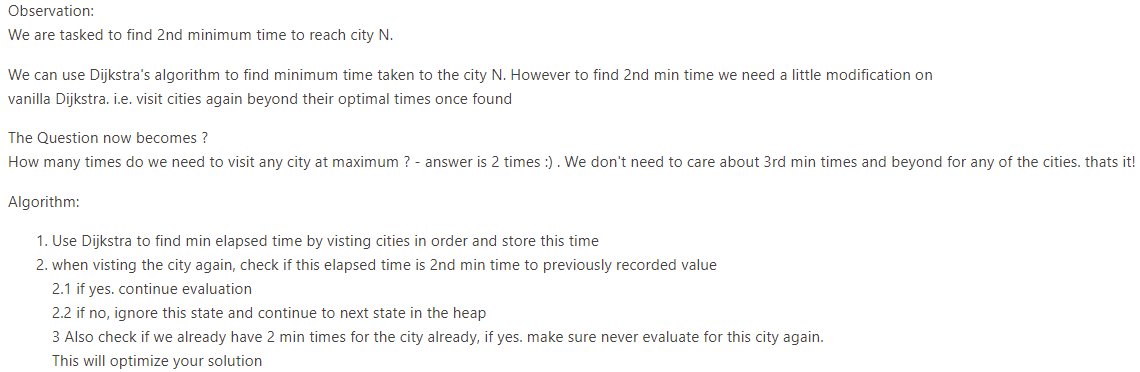
\includegraphics[width=.9\linewidth]{./pic/redGreen.png}

\begin{minted}[fontsize=\scriptsize,linenos=false]{csharp}
public int secondMinimum(int n, int[][] edges, int time, int change) {
    Map<Integer, List<Integer>> adj = new HashMap<>();
    for (int [] e : edges) {
        adj.computeIfAbsent(e[0], z -> new ArrayList<>()).add(e[1]);
        adj.computeIfAbsent(e[1], z -> new ArrayList<>()).add(e[0]);
    }
    Queue<int []> q = new PriorityQueue<>((a, b)->(a[1] -b[1]));
    q.offer(new int []{1, 0});
    Map<Integer, Integer> cache = new HashMap<>(); // use cache tmpo record min time per city
    // modification: we want to visit each city maximum two times with different times,
    // this will help in early termination when we visit the city again (3rd time or more)
    Set<Integer> exhausted = new HashSet<>();
    while (!q.isEmpty()) {
        int [] top = q.poll();
        int cur = top[0], t = top[1];
        // Base Termination : we have found our 2nd min time for city n
        if (cur == n && t > cache.getOrDefault(cur, Integer.MAX_VALUE))
            return t;
        if (!cache.containsKey(cur)) // we vistied this city for first time, so elapsed time is min for this city
            cache.put(cur, t);
        // early termination, if we are trying to visit the city 3rd time or more ,
        // or the elapsed time will not help in finding the solution
        else if (cache.get(cur) == t || exhausted.contains(cur)) continue;
        else // this means we are visiting the city with 2nd optimal time , we dont need to visit the city ever again
            exhausted.add(cur);
        // we visit the city on elapsedTime, we need to check if on basis of change time, whether this time falls in  cycle (green or red)
        // if odd cycle (red), we must wait for this cycle to end
        int factor = t / change;
        if (factor % 2 == 1)
            t = (factor + 1) * change;
        for (int nb : adj.getOrDefault(cur, new ArrayList<>())) { // visit the neighbours
            int visTime = t + time;
            if (!exhausted.contains(nb))
                q.offer(new int [] {nb, visTime});
        }
    }
    return -1;
}
\end{minted}
\begin{itemize}
\item 另一个也是写得直接了当的
\end{itemize}
\begin{minted}[fontsize=\scriptsize,linenos=false]{csharp}
public int secondMinimum(int n, int [][] edges, int time, int change) {
    Map<Integer, Set<Integer>> map = new HashMap<>();
    for (int [] e : edges) {
        map.computeIfAbsent(e[0], z -> new HashSet<>()).add(e[1]);
        map.computeIfAbsent(e[1], z -> new HashSet<>()).add(e[0]);
    }
    Queue<int []> q = new PriorityQueue<>((a, b)->(a[1]-b[1]));
    Map<Integer, Set<Integer>> vis = new HashMap<>();
    q.offer(new int [] {1, 0});
    int min = -1;
    while (!q.isEmpty()) {
        int [] top = q.poll();
        int cur = top[0], t = top[1];
        if (cur == n) {
            if (min == -1 || min == t) min = t;
            else return t;
        }
        if (t % (2 * change) >= change)
            t += 2 * change - t % (2 * change);
        // 源码中传入key和value,根据key获取看是否存在value,如果value==null,然后调用put方法把传入的key和value  put进map,返回根据key获取的老value
        // 如果传入key对应的value已经存在,就返回存在的value,不进行替换。如果不存在,就添加key和value,返回null
        vis.putIfAbsent(cur, new HashSet<>());
        if (!vis.get(cur).add(t) || vis.get(cur).size() >= 3) continue;
        if (map.containsKey(cur))
            for (int next : map.get(cur)) 
                q.offer(new int [] {next, t + time});
    }
    return -1;
}
\end{minted}

\subsection{1334. Floyd算法 - Find the City With the Smallest Number of Neighbors at a Threshold Distance - Medium}
\label{sec-12-1-4}
There are n cities numbered from 0 to n-1. Given the array edges where edges[i] = [fromi, toi, weighti] represents a bidirectional and weighted edge between cities fromi and toi, and given the integer distanceThreshold.

Return the city with the smallest number of cities that are reachable through some path and whose distance is at most distanceThreshold, If there are multiple such cities, return the city with the greatest number.

Notice that the distance of a path connecting cities i and j is equal to the sum of the edges' weights along that path.
\begin{minted}[fontsize=\scriptsize,linenos=false]{csharp}
public int findTheCity(int n, int[][] edges, int distanceThreshold) {
    // 1.创建邻接矩阵
    int [][] graph = new int [n][n]; // 相比于我只会用HashMap来建邻接关系,邻接链表与数组都可能,看哪个用起来方便
    for (int i = 0; i < n; i++)
        Arrays.fill(graph[i], Integer.MAX_VALUE); // pre filled n equaivlent to Integer.MAX_VALUE
    for (int [] eg : edges) {
        graph[eg[0]][eg[1]] = eg[2];
        graph[eg[1]][eg[0]] = eg[2];
    }
    // 2.floyd算法
    for (int k = 0; k < n; k++)          // 中间结点
        for (int i = 0; i < n; i++)      // 开始结点
            for (int j = 0; j < n; j++) {// 结尾结点
                if (i == j || graph[i][k] == Integer.MAX_VALUE || graph[k][j] == Integer.MAX_VALUE) continue;
                graph[i][j] = Math.min(graph[i][j], graph[i][k] + graph[k][j]);
            }                
    // 3.每个城市距离不大于distanceThreshold的邻居城市的数目
    int [] mark = new int [n]; //记录小于distanceThreshold的邻居城市个数
    for (int i = 0; i < n; i++) 
        for (int j = 0; j < n; j++) 
            if (graph[i][j] <= distanceThreshold)
                mark[i]++;
    // 4.找数目少,编号最大的
    int min = n;
    int ans = 0;
    for (int i = 0; i < n; i++) 
        if (min >= mark[i]) {
            min = mark[i];
            ans = i;
        }
    return ans;
}
\end{minted}
\begin{itemize}
\item 另一种解法
\end{itemize}
\begin{minted}[fontsize=\scriptsize,linenos=false]{csharp}
// 之前用原创想法也写了很多图的题,但缺乏归纳总结,原创想法更多的是解决了题目,但解法与效率、与优化算法间的距离还需要很多比较归纳与总结,才能把图这一块吃透
// https://leetcode.jp/leetcode-1334-find-the-city-with-the-smallest-number-of-neighbors-at-a-threshold-distance-%E8%A7%A3%E9%A2%98%E6%80%9D%E8%B7%AF%E5%88%86%E6%9E%90/  这个题需要重新写
// map:图结构
// city:当前城市
// dis:当前所剩距离
// v:已经被记录为邻居的节点
// maxDis:走到某个节点时,剩余距离的最大值
// 返回值为当前城市的邻居数。
private int dfs(int [][] arr, int city, int dis, boolean [] vis, int [] maxDis) {
    int res = 0;
    for (int i = 0; i < arr[0].length; i++) { // 循环当前城市的所有相邻城市
        int distance = arr[city][i]; // 与相邻城市的距离,如果为0,说明与该城市不相连
        int diffDis = dis - distance;// 到达相邻城市后,与阈值相比的剩余距离。
        if (distance > 0 && diffDis >= maxDis[i]) { // 与该城市相连并且剩余距离大于等于访问数组中的值
            maxDis[i] = diffDis;     // 更新访问数组中的剩余距离   
            if (!vis[i]) {
                vis[i] = true;
                res++;
            }
            res += dfs(arr, i, diffDis, vis, maxDis); // 递归dfs与该城市相连的其他城市:图中我似乎还很没有dfs以及递归的概念
        }
    }
    return res;
}
public int findTheCity(int n, int[][] edges, int distanceThreshold) {
    int [][] map = new int [n][n];
    for (int [] eg : edges) {
        map[eg[0]][eg[1]] = eg[2];
        map[eg[1]][eg[0]] = eg[2];
    }
    int min = n;
    int res = 0;
    for (int i = 0; i < n; i++) {
        boolean [] vis = new boolean [n];
        vis[i] = true;
        int cnt = dfs(map, i, distanceThreshold, vis, new int [n]);
        if (cnt <= min) {
            min = cnt;
            res = i;
        }
    }
    return res;
}
\end{minted}

\subsection{1129. Shortest Path with Alternating Colors - Medium}
\label{sec-12-1-5}
Consider a directed graph, with nodes labelled 0, 1, \ldots{}, n-1.  In this graph, each edge is either red or blue, and there could be self-edges or parallel edges.

Each [i, j] in red\_edges denotes a red directed edge from node i to node j.  Similarly, each [i, j] in blue\_edges denotes a blue directed edge from node i to node j.

Return an array answer of length n, where each answer[X] is the length of the shortest path from node 0 to node X such that the edge colors alternate along the path (or -1 if such a path doesn't exist).
\begin{minted}[fontsize=\scriptsize,linenos=false]{csharp}
// 找最短路径应该用queue来做,入队列的时候需要标记红边或是蓝边以便找交替路径
public int[] shortestAlternatingPaths(int n, int[][] red_edges, int[][] blue_edges) {
    HashMap<Integer, List<Integer>> [] maps = new HashMap [2]; // 0 : red; 1: blue
    for (int i = 0; i < 2; i++) 
        maps[i] = new HashMap<>();
    for (int i = 0; i < red_edges.length; i++) 
        maps[0].computeIfAbsent(red_edges[i][0], k->new ArrayList<>()).add(red_edges[i][1]);
    for (int i = 0; i < blue_edges.length; i++) 
        maps[1].computeIfAbsent(blue_edges[i][0], k->new ArrayList<>()).add(blue_edges[i][1]);
    int [] ans = new int[n];
    Arrays.fill(ans, -1);
    Queue<int []> q = new LinkedList<>();
    q.offer(new int [] {0, 0}); // red edge         
    q.offer(new int [] {0, 1}); // blue edge
    boolean [][] inQueue = new boolean [n][2]; // 0: red, 1: blue
    inQueue[0][0] = true;
    inQueue[0][1] = true;
    int cnt = 0, color = 0;
    while (!q.isEmpty()) {
        for (int size = q.size(); size > 0; size--) {
            int [] cur = q.poll();
            System.out.println(Arrays.toString(cur));
            color = cur[1];
            if (ans[cur[0]] == -1) ans[cur[0]] = cnt;
            List<Integer> nextNodes = maps[1-color].get(cur[0]);
            if (nextNodes == null) continue;
            for (Integer next : nextNodes) 
                if (!inQueue[next][1-color]) {
                    q.offer(new int [] {next, 1-color});
                    inQueue[next][1-color] = true;
                }
        }
        ++cnt;
    }
    return ans;
}
\end{minted}
\begin{itemize}
\item 不是总喜欢省掉大括号吗,试试省掉下面的。。。。。。
\end{itemize}
\begin{minted}[fontsize=\scriptsize,linenos=false]{csharp}
public int[] shortestAlternatingPaths(int n, int[][] red_edges, int[][] blue_edges) {
    int [][] red = new int[n][2]; // 红 0 蓝 1
    int [][] blue = new int[n][2];
    for (int i = 1; i < n; i++) {
        red[i][0] = i;
        red[i][1] = 0x0fffffff;   // 初始化红边权值
    }
    red [0][0] = 0;
    red [0][1] = 0;
    for (int i = 1; i < n; i++) {
        blue[i][0] = i;
        blue[i][1] = 0x0fffffff;
    }
    blue [0][0] = 0;
    blue [0][1] = 0;
    dfs(red, blue, 0, 0, red_edges, blue_edges);
    dfs(red, blue, 1, 0, red_edges, blue_edges);
    int [] ans = new int[n];
    for(int i = 0; i < n; i++){
        ans[i] = Math.min(red[i][1], blue[i][1]);
        if (ans[i] == 0x0fffffff) // 没有改变说明不存在
            ans[i] = -1;
    }
    return ans;
}
public void dfs(int [][] red, int [][] blue, int color, int node, int[][] red_edges, int[][] blue_edges){
    if (color == 0) { // 这个括号可以省吗???
        for (int [] blue_to : blue_edges) // 以node为from to 为终 的边
            if (node == blue_to[0] && red[node][1]+1 < blue[blue_to[1]][1]) {// 0到from点加1是否小于0到to的距离
                blue[blue_to[1]][1] = red[node][1]+1; // 作距离的更新
                dfs(red, blue, 1-color, blue_to[1], red_edges, blue_edges);
            }
    } else for (int [] red_to : red_edges) //以node为from to 为终 的边
               if (node == red_to[0] && blue[node][1]+1 < red[red_to[1]][1]) {//0到from点加1是否小于0到to的距离
                   red[red_to[1]][1] = blue[node][1]+1;
                   dfs(red, blue, 1-color, red_to[1], red_edges, blue_edges);
               }
}
\end{minted}

\subsection{882. Reachable Nodes In Subdivided Graph - Hard}
\label{sec-12-1-6}
You are given an undirected graph (the "original graph") with n nodes labeled from 0 to n - 1. You decide to subdivide each edge in the graph into a chain of nodes, with the number of new nodes varying between each edge.

The graph is given as a 2D array of edges where edges[i] = [ui, vi, cnti] indicates that there is an edge between nodes ui and vi in the original graph, and cnti is the total number of new nodes that you will subdivide the edge into. Note that cnti == 0 means you will not subdivide the edge.

To subdivide the edge [ui, vi], replace it with (cnti + 1) new edges and cnti new nodes. The new nodes are x1, x2, \ldots{}, xcnti, and the new edges are [ui, x1], [x1, x2], [x2, x3], \ldots{}, [xcnti-1, xcnti], [xcnti, vi].

In this new graph, you want to know how many nodes are reachable from the node 0, where a node is reachable if the distance is maxMoves or less.

Given the original graph and maxMoves, return the number of nodes that are reachable from node 0 in the new graph.

再进一步来分析,其实上对于每个结点来说(不论有没有编号),若我们能算出该结点离起始结点的最短距离,且该距离小于等于M的话,那这个结点就一定可以到达。这样来说,其实本质就是求单源点的最短距离,此时就要祭出神器迪杰斯特拉算法 Dijkstra Algorithm 了,LeetCode 中使用了该算法的题目还有 Network Delay Time 和 The Maze II。该算法的一般形式是用一个最小堆来保存到源点的最小距离,这里我们直接统计到源点的最小距离不是很方便,可以使用一个小 trick,即用一个最大堆来统计当前结点所剩的最大步数,因为剩的步数越多,说明距离源点距离越小。由于 Dijkstra 算法是以起点为中心,向外层层扩展,直到扩展到终点为止。根据这特性,用 BFS 来实现时再好不过了,首先来建立邻接链表,这里可以使用一个 NxN 的二维数组 graph,其中 graph[i][j] 表示从大结点i往大结点j方向会经过的小结点个数,建立邻接链表的时候对于每个 edge,要把两个方向都赋值,前面解释过了这里要当作有向图来做。然后使用一个最大堆,里面放剩余步数和结点编号组成的数对儿,把剩余步数放前面就可以默认按步数从大到小排序了,初始化时把 \{M,0\} 存入最大堆。还需要一个一维数组 visited 来记录某个结点是否访问过。

\begin{minted}[fontsize=\scriptsize,linenos=false]{csharp}
public int reachableNodes(int[][] edges, int maxMoves, int n) {
    int [][] graph = new int  [n][n];
    for (int i = 0; i < n; i++) 
        Arrays.fill(graph[i], -1);
    for (int [] v : edges) {
        graph[v[0]][v[1]] = v[2];
        graph[v[1]][v[0]] = v[2];
    }
    Queue<int []> q = new PriorityQueue<>((a, b) -> (b[0] - a[0]));
    boolean [] vis = new boolean [n];
    q.offer(new int [] {maxMoves, 0});
    int res = 0;
    while (!q.isEmpty()) {
        int [] cur = q.poll();
        int cnt = cur[0], u = cur[1];
        if (vis[u]) continue;
        vis[u] = true;
        ++res;
        for (int i = 0; i < n; i++) {
            if (graph[u][i] == -1) continue;
            if (cnt > graph[u][i] && !vis[i])
                q.offer(new int [] {cnt - graph[u][i]-1, i});
            graph[i][u] -= Math.min(cnt, graph[u][i]);
            res += Math.min(cnt, graph[u][i]);
        }
    }
    return res;
}
\end{minted}
\begin{itemize}
\item 我们也可以使用 HashMap 来建立邻接链表,最后的运行速度果然要比二维数组形式的邻接链表要快一些,其他的地方都不变,参见代码如下:
\end{itemize}
\begin{minted}[fontsize=\scriptsize,linenos=false]{csharp}
public int reachableNodes(int[][] edges, int maxMoves, int n) {
    int res = 0;
    Map<Integer, Map<Integer, Integer>> graph = new HashMap<>();
    for (int [] v : edges) {
        graph.computeIfAbsent(v[0], k->new HashMap<>()).put(v[1], v[2]);
        graph.computeIfAbsent(v[1], k->new HashMap<>()).put(v[0], v[2]);
    }
    Queue<int []> q = new PriorityQueue<>((a, b) -> (b[0] - a[0]));
    boolean [] vis = new boolean [n];
    q.offer(new int [] {maxMoves, 0});
    while (!q.isEmpty()) {
        int [] cur = q.poll();
        int cnt = cur[0], u = cur[1];
        if (vis[u]) continue;
        vis[u] = true;
        ++res;
        for (int i = 0; i < n; i++) {
            if (!graph.containsKey(u) || !graph.get(u).containsKey(i) || graph.get(u).get(i) == -1) continue;
            if (cnt > graph.get(u).get(i) && !vis[i])
                q.offer(new int [] {cnt - graph.get(u).get(i)-1, i});
            graph.get(i).put(u, graph.get(u).get(i) - Math.min(cnt, graph.get(u).get(i)));
            res += Math.min(cnt, graph.get(u).get(i));
        }
    }
    return res;
}
\end{minted}

\subsection{1782. Count Pairs Of Nodes - Hard}
\label{sec-12-1-7}
You are given an undirected graph defined by an integer n, the number of nodes, and a 2D integer array edges, the edges in the graph, where edges[i] = [ui, vi] indicates that there is an undirected edge between ui and vi. You are also given an integer array queries.

Let incident(a, b) be defined as the number of edges that are connected to either node a or b.

The answer to the jth query is the number of pairs of nodes (a, b) that satisfy both of the following conditions:

a < b
incident(a, b) > queries[j]
Return an array answers such that answers.length == queries.length and answers[j] is the answer of the jth query.

Note that there can be multiple edges between the same two nodes.
\begin{minted}[fontsize=\scriptsize,linenos=false]{csharp}
// https://leetcode.com/problems/count-pairs-of-nodes/discuss/1096740/C%2B%2BJavaPython3-Two-Problems-O(q-*-(n-%2B-e))
public int[] countPairs(int n, int[][] edges, int[] queries) { // 别人家的思路好清晰
    int [] cnt = new int [n+1], sortedCnt = new int [n+1], ans = new int [queries.length];
    Map<Integer, Integer> [] m = new HashMap[n+1];
    for (var e : edges) {
        sortedCnt[e[0]] = cnt[e[0]] = cnt[e[0]] + 1;
        sortedCnt[e[1]] = cnt[e[1]] = cnt[e[1]] + 1;
        int min = Math.min(e[0], e[1]), max = Math.max(e[0], e[1]);
        m[min] = m[min] == null ? new HashMap<>() : m[min];
        m[min].put(max, m[min].getOrDefault(max, 0) + 1); // 仍然是当作有向图、单向图来做
    }
    Arrays.sort(sortedCnt);
    int res = 0, cur = 0;
    for (int k = 0; k < queries.length; k++) {
        for (int i = 1, j = n; i < j;) 
            if (queries[k] < sortedCnt[i] + sortedCnt[j])
                ans[k] += (j--) - i;
            else ++i;
        for (int i = 1; i <= n; i++) 
            if (m[i] != null) 
                for (var en : m[i].entrySet()) {
                    int j = en.getKey(), sharedCnt = en.getValue();
                    if (queries[k] < cnt[i] + cnt[j] && cnt[i] + cnt[j] - sharedCnt <= queries[k])
                        ans[k]--;
                }
    } 
    return ans;
}
\end{minted}

\subsection{2115. Find All Possible Recipes from Given Supplies}
\label{sec-12-1-8}
You have information about n different recipes. You are given a string array recipes and a 2D string array ingredients. The ith recipe has the name recipes[i], and you can create it if you have all the needed ingredients from ingredients[i]. Ingredients to a recipe may need to be created from other recipes, i.e., ingredients[i] may contain a string that is in recipes.

You are also given a string array supplies containing all the ingredients that you initially have, and you have an infinite supply of all of them.

Return a list of all the recipes that you can create. You may return the answer in any order.

Note that two recipes may contain each other in their ingredients.
\begin{enumerate}
\item 解题思路与分析
\label{sec-12-1-8-1}
\begin{minted}[fontsize=\scriptsize,linenos=false]{csharp}
public List<String> findAllRecipes(String[] re, List<List<String>> ing, String[] sup) { // 菜谱 菜谱原材料 食材 BUG BUG BUG
    Map<String, Set<String>> adj = new HashMap<>();    // 每种材料可以做成的菜的 清单
    Map<String, Integer> ins = new HashMap<>();        // 每种材料或是菜谱的 入度
    for (int i = 0; i < re.length; i++) 
        for (String it : ing.get(i)) {
            adj.computeIfAbsent(it, z -> new HashSet<>()).add(re[i]);
            ins.put(re[i], ins.getOrDefault(re[i], 0) + 1);
        }
    List<String> ans = new ArrayList<>();
    Deque<String> q = new ArrayDeque<>();
    for (String s : sup) q.offerLast(s); // 把初始的原材料放入队列
    while (!q.isEmpty()) { // 拓扑排序
        String cur = q.pollFirst();
        if (adj.containsKey(cur)) 
            for (String one : adj.get(cur)) { // 遍历某种原材料可以做成的所有的菜,其入度是否为0
                ins.put(one, ins.get(one)-1); // 入度 ins--
                if (ins.get(one) == 0) {
                    ans.add(one);
                    q.offerLast(one);
                }
            }
    }
    return ans;
}
\end{minted}
\end{enumerate}

\section{基环内向树}
\label{sec-12-2}
\subsection{2127. Maximum Employees to Be Invited to a Meeting - Hard 基环内向树}
\label{sec-12-2-1}
A company is organizing a meeting and has a list of n employees, waiting to be invited. They have arranged for a large circular table, capable of seating any number of employees.

The employees are numbered from 0 to n - 1. Each employee has a favorite person and they will attend the meeting only if they can sit next to their favorite person at the table. The favorite person of an employee is not themself.

Given a 0-indexed integer array favorite, where favorite[i] denotes the favorite person of the ith employee, return the maximum number of employees that can be invited to the meeting.
\begin{enumerate}
\item 解题思路与分析
\label{sec-12-2-1-1}
如果我们把每个员工看成图上的一个节点,如果员工 xx 喜欢员工 yy,就在从 xx 对应的节点到 yy 对应的节点连一条边,那么形成的图是什么结构的?形成的图会由若干颗「基环内向树」组成。所谓「基环内向树」,就是形如下图所示的结构:

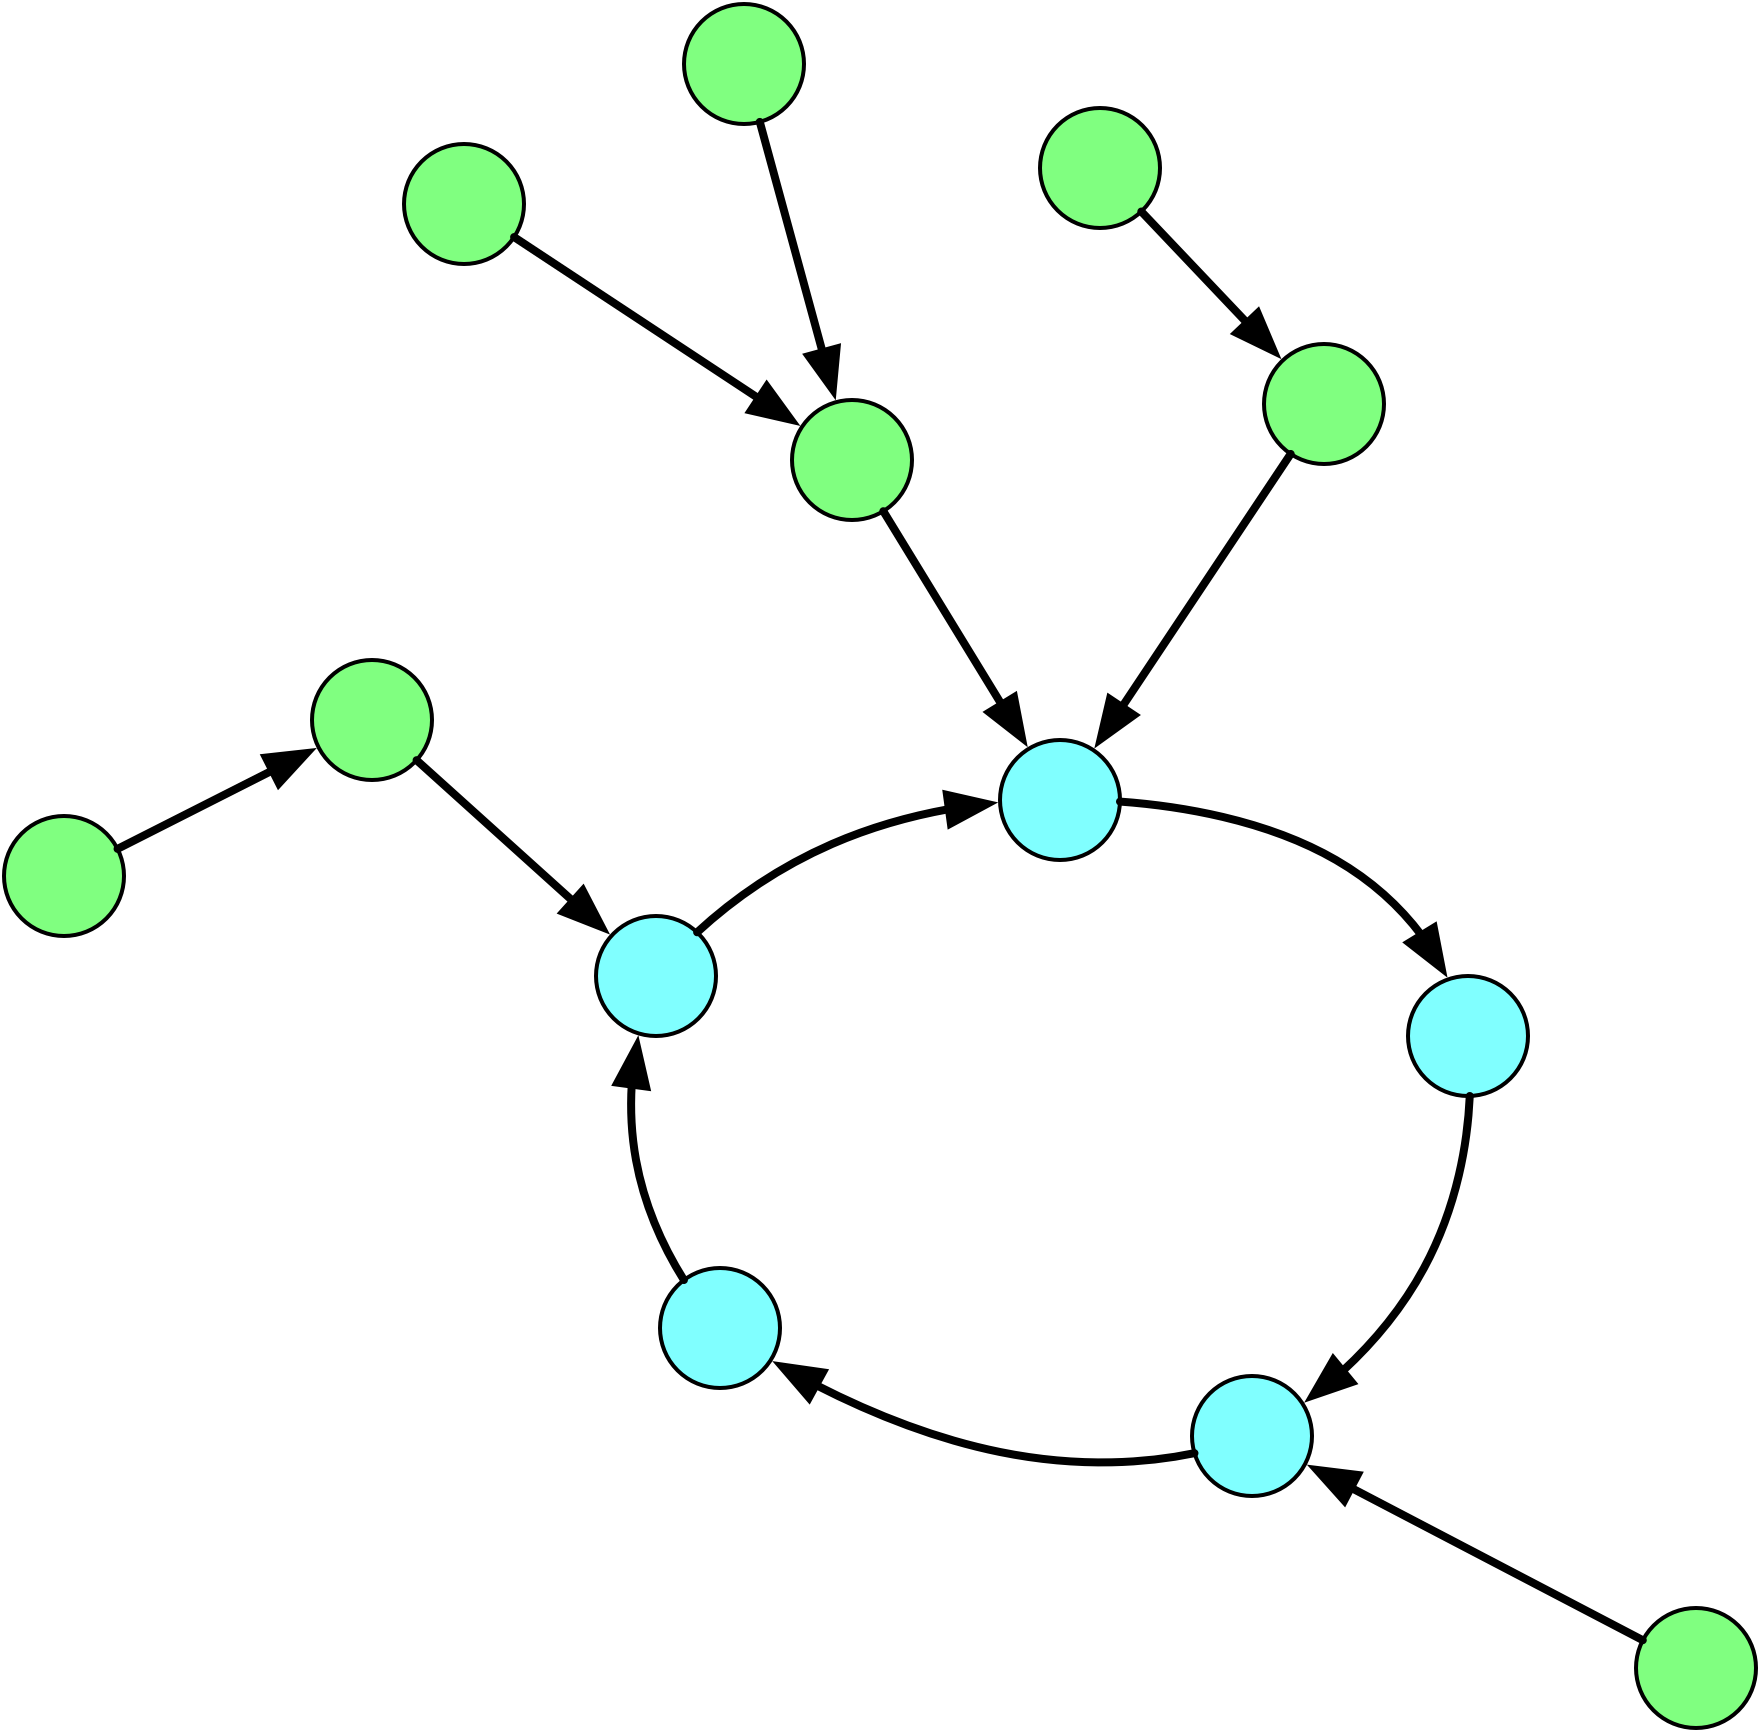
\includegraphics[width=.9\linewidth]{./pic/2277tree-1.png}


我们从任意一个节点 xx 开始在图上进行「游走」,由于每个员工只有一位喜欢的员工,因此每个节点在图上只会有一条出边,即「游走」的过程是唯一的。由于图上有 nn 个节点,因此在 n+1n+1 步以内,一定会走到一个重复的节点,那么在第一次经过该节点之后,到第二次经过该节点之前的所有节点,以及该节点本身,就组成了一个环,如上图的蓝色节点所示。

对于不在环上的节点,我们已经说明了从它们开始「游走」也一定会进入到环中。在到达环上的节点之前,它们不会重复经过节点(否则就有两个环了,我们可以证明一个连通分量中是不可能有两个环的:因为每个节点只有一条出边,因此如果有两个环并且它们连通,那么必然某个环上有一个点有两条出边,一条出边指向同一个环上的节点,另一条出边可以使得它到达另一个环,这就产生了矛盾),那么它们就形成了类似树的结构,如上图的绿色节点所示。

需要注意的是,一个单独的环也是「基环内向树」,它是一种特殊情况,即没有绿色的节点。

思路与算法

既然我们知道了图由若干颗「基环内向树」组成,那么我们就可以想一想,每一颗「基环内向树」的哪一部分可以被安排参加会议。

我们首先讨论特殊的情况,即一个单独的环(或若干个环),并且所有环的大小都 $\ge$ 3≥3。可以发现,我们按照环上的顺序给对应的员工安排座位是满足要求的,因为对于每一个环上的员工,它喜欢的员工就在它的旁边。并且,我们必须安排环上的所有员工,因为如果有缺失,那么喜欢那位缺失了的员工的员工就无法满足要求了。

但如果我们已经安排了某一个环上的所有员工,剩余的环就没有办法安排了。这是因为已经安排的那个环是没有办法被「断开」的:断开的本质就是相邻位置员工的缺失。因此,我们可以得出一个重要的结论:

如果我们想安排大小 $\ge$ 3≥3 的环,我们最多只能安排一个,并且环需要是完整的。

那么如果是环大小 $\ge$ 3≥3 的「基环内向树」呢?如果我们安排了不在环上的节点,那么从该节点开始,我们需要不断安排当前节点喜欢的员工,这实际上就是「游走」的过程。而当我们游走到环上并到达环上最后一个未经过的节点时,该节点的下一个节点(即喜欢的员工)已经被安排过,所以最后一个未经过的节点就无法被安排,不满足要求。因此,我们不能安排任何不在环上的节点,只能安排在环上的节点,就得出了另一个的结论:

所有环大小 $\ge$ 3≥3 的「基环内向树」与一个大小相同(指环的部分)的环是等价的。

那么最后我们只需要考虑大小 =2=2 的环或者「基环内向树」了。这里的特殊之处在于,大小 =2=2 的环可以安排多个:因为环上的两个点是互相喜欢的,因此只需要它们相邻即可,而没有其它的要求。而对于环大小 =2=2 的「基环内向树」,如果我们安排了不在环上的节点,那么游走完环上两个节点之后,同样是满足要求的,并且我们甚至可以继续延伸(反向「游走」),到另一个不在环上的节点为止。如下图所示,包含 \texttt{X}X 的节点就是可以安排参加会议的节点。

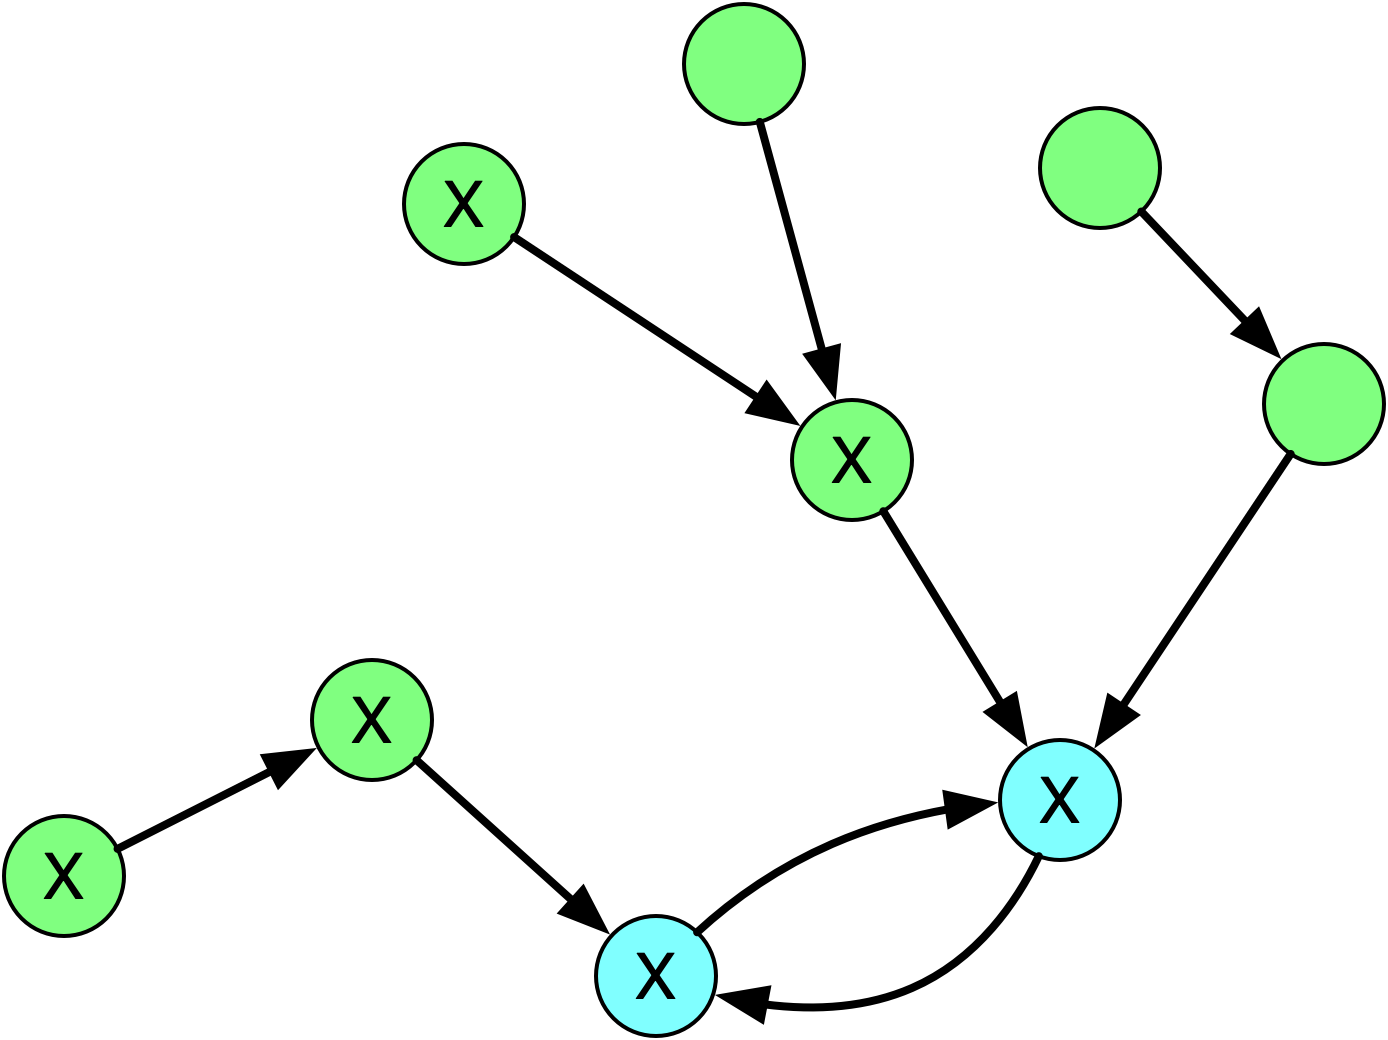
\includegraphics[width=.9\linewidth]{./pic/2277tree-2.png}

并且同样地,对于每一棵环大小 =2=2 的「基环内向树」,我们都可以取出这样一条「双向游走」路径进行安排,它们之间不会影响。综上所述,原问题的答案即为下面二者中的最大值:

最大的环的大小;

所有环大小 =2=2 的「基环内向树」上的最长的「双向游走」路径之和。

为了求解「基环内向树」上的最长的「双向游走」路径,我们可以使用拓扑排序 + 动态规划的方法。记 f[i]f[i] 表示到节点 ii 为止的最长「游走」路径经过的节点个数,那么状态方程即为:

即我们考虑节点 ii 的上一个节点 jj,在图中必须有从 jj 到 ii 的一条有向边,这样我们就可以从 jj 转移到 ii。如果不存在满足要求的 jj(例如「基环内向树」退化成一个大小 =2=2 的环),那么 f[i] = 1f[i]=1。状态转移可以和拓扑排序同时进行。

在拓扑排序完成后,剩余没有被弹出过队列的节点就是环上的节点。我们可以找出每一个环。如果环的大小 $\ge$ 3≥3,我们就用其来更新最大的环的大小;如果环的大小 =2=2,设环上的两个节点为 xx 和 yy,那么该「基环内向树」上最长的「双向游走」的路径长度就是 f[x] + f[y]f[x]+f[y]。

\begin{minted}[fontsize=\scriptsize,linenos=false]{csharp}
public int maximumInvitations(int[] a) { // a: favorite
    // 统计入度,便于进行拓扑排序
    int n = a.length, ins [] = new int [n];
    for (int v : a) ins[v]++;
    boolean vis [] = new boolean [n];
    int f [] = new int [n];
    Arrays.fill(f, 1);
    Deque<Integer> q = new ArrayDeque<>();
    for (int i = 0; i < n; i++) 
        if (ins[i] == 0) q.offerLast(i); 
    while (!q.isEmpty()) {
        int u = q.pollFirst();
        vis[u] = true;
        int v = a[u];
        f[v] = Math.max(f[v], f[u] + 1); // 动态规划: 能够到达 v 的最长链的长度
        --ins[v];
        if (ins[v] == 0) q.offerLast(v);
    }
    // ring 表示最大的环的大小
    // total 表示所有环大小为 2 的「基环内向树」上的最长的「双向游走」路径之和
    int ring = 0, total = 0;
    for (int i = 0; i < n; i++) {
        if (!vis[i]) {
            int j = a[i];
            if (a[j] == i) { // 说明环的大小为 2
                total += f[i] + f[j]; // 局部二元环可以叠加
                vis[i] = vis[j] = true;
            } else { // 否则环的大小至少为 3,我们需要找出环
                int u = i, cnt = 0;
                do { // 至少执行一次,evaluate after execute
                    ++cnt;
                    u = a[u];
                    vis[u] = true;
                } while (u != i); // 再达到达这一点,说明转了一圈,又回到了起点
                ring = Math.max(ring, cnt); // 找出一个节点数目最多的环
            }
        }
    }
    return Math.max(ring, total);
}
\end{minted}
\end{enumerate}
\section{Tarjan 算法}
\label{sec-12-3}
\begin{itemize}
\item 图的一些基本概念:
\item \textbf{关联(incident)} : 点为边的端点;
\item \textbf{邻接(adjacent)} : 点与点关联同一条边,或边与边关联同一顶点;
\item \textbf{子图} : 图G'的点和边都是图G的子集,则G'为G的子图;
\item \textbf{道路} : 从点v到点u的路径;
\begin{itemize}
\item \textbf{简单道路} : 没有重复边的道路;
\item \textbf{回路} : 起点与终点相同的道路;
\item \textbf{简单回路} : 没有重复边的回路;
\item \textbf{连通} : 两顶点间有道路;
\item \textbf{强连通} : 有向图u→v与v→u都有道路;
\item \textbf{连通图} : 任意两顶点间都有道路(若有向图除去方向后连通,则称有向图连通);
\item \textbf{简单图} : 没有重复边和自环的图;
\item \textbf{完全图} : 任意两顶点间有一条边到达的简单图(有向完全图与无向完全图);
\item \textbf{强连通(strongly connected)} : 在有向图G 中,如果两个顶点间至少存在一条路径,称两个顶点强连通(strongly connected);
\item \textbf{强连通图} : 如果有向图G 的每两个顶点都强连通,称G 是一个强连通图;
\item \textbf{强连通分量(strongly connected components)} : 非强连通图有向图的极大强连通子图,称为强连通分量(strongly connected components)。
\end{itemize}
\item 无向图的割点与桥
\begin{itemize}
\item 什么是无向图?简单来说,若一个图中每条边都是无方向的,则称为无向图。
\item 割点: 若从图中删除节点 x 以及所有与 x 关联的边之后,图将被分成两个或两个以上的不相连的子图,那么称 x 为图的割点。
\item 桥: 若从图中删除边 e 之后,图将分裂成两个不相连的子图,那么称 e 为图的桥或割边。
\end{itemize}
\item 求强连通分量就是我们今天要解决的问题,根据强连通分量定义,用双向遍历取交集的方法求强连通分量,时间复杂度为O(\$N\^{}2\$+M). 而Tarjan或Kosaraju算法, 两者的时间复杂度都是O(N+M)。
\end{itemize}
\subsection{算法简介}
\label{sec-12-3-1}

在了解了 Tarjan 算法的背景以及图的割点与桥的基本概念之后,我们下面所面临的问题就是 —— 如何求解图的割点与桥?

开门见山,我们直接引出 Tarjan 算法在求解无向图的割点与桥的工作原理。

\begin{itemize}
\item 时间戳: ​时间戳是用来标记图中每个节点在进行深度优先搜索时被访问的时间顺序,当然,你可以理解成一个序号(这个序号由小到大),用 dfn[x] 来表示。
\item 搜索树: 在无向图中,我们以某一个节点 x 出发进行深度优先搜索,每一个节点只访问一次,所有被访问过的节点与边构成一棵树,我们可以称之为“无向连通图的搜索树”。
\item 追溯值: 追溯值用来表示从当前节点 x 作为搜索树的根节点出发,能够访问到的所有节点中,时间戳最小的值 —— low[x]。那么,我们要限定下什么是“能够访问到的所有节点”?,其需要满足下面的条件之一即可:
\begin{itemize}
\item 以 x 为根的搜索树的所有节点
\item 通过一条非搜索树上的边,能够到达搜索树的所有节点
\end{itemize}
\end{itemize}

Tarjan 算法是基于对图深度优先搜索的算法,每个强连通分量为搜索树中的一棵子树。搜索时,把当前搜索树中未处理的节点加入一个堆栈,回溯时可以判断栈顶到栈中的节点是否为一个强连通分量。

\begin{itemize}
\item 定义:
\begin{itemize}
\item o DFN(u)为节点u 搜索的次序编号(时间戳);
\item o LOW(u)为u 或 u的子树能够追溯到的最早的栈中节点的次序号;
\end{itemize}
\end{itemize}

由定义可以得出,当 DFN(u)=LOW(u)时,以u为根的搜索子树上所有节点是一个强连通分量。

\begin{itemize}
\item 算法:
\begin{itemize}
\item 当首次搜索到点u时DFN[u]=LOW[u]=time;
\item 每当搜索到一个点,把该点压入栈顶;
\item 当u和v有边相连时:
\end{itemize}
\end{itemize}

1)如果v不在栈中(树枝边),DFS(v),并且LOW[u] = min\{LOW(u),LOW(v)\};

2)如果v在栈中(前向边/后向边),此时LOW[u] = min\{LOW[u],DFN[v]\}
\begin{itemize}
\item 当DFN[u]=LOW[u]时,将它以及在它之上的元素弹出栈,此时,弹出栈的结点构成一个强连通分量;
\item 继续搜索,知道图被遍历完毕。
\end{itemize}

由于在这个过程中每个点只被访问一次,每条边也只被访问一次,所以Tarjan算法的时间复杂度是O(n+m).

\begin{itemize}
\item 这个算法需要用到好几个辅助数组, 下面我来详细介绍它们的作用
\begin{itemize}
\item int dfn[MAXN];// 用来记录一个顶点第一次被访问时的时间戳
\item int low[MAXN];// 用来记录一个顶点不经过它的父亲顶点最高能访问到它的祖先节点中的最小时间戳, 通俗易懂的来说, 就是与结点i连接的所有点中dfn[]值最小的一个。
\item int cut[MAXN];// 用来记录该点是否是割点, 因为一个割点可能多次被记录
\end{itemize}
\end{itemize}

\subsection{1192. Critical Connections in a Network- Hard Tarjan 算法 Tarjan's algorithm Kosaraju算法 -- todo: 这个题不太懂}
\label{sec-12-3-2}
There are n servers numbered from 0 to n - 1 connected by undirected server-to-server connections forming a network where connections[i] = [ai, bi] represents a connection between servers ai and bi. Any server can reach other servers directly or indirectly through the network.

A critical connection is a connection that, if removed, will make some servers unable to reach some other server.

Return all critical connections in the network in any order.
\begin{enumerate}
\item 解题思路与分析
\label{sec-12-3-2-1}
\begin{itemize}
\item \url{https://www.cnblogs.com/nullzx/p/7968110.html}

\begin{minted}[fontsize=\scriptsize,linenos=false]{csharp}
public List<List<Integer>> criticalConnections(int n, List<List<Integer>> connections) {
    depth = new int [n];
    Arrays.fill(depth, -1);
    adj = new ArrayList[n]; // 初始化结构图map[i]代表节点i可以连通哪些节点
    for (int i = 0; i < n; i++) adj[i] = new ArrayList<>();
    for (List<Integer> c : connections) {
        adj[c.get(0)].add(c.get(1));
        adj[c.get(1)].add(c.get(0));
    }
    dfs(0, 0, 0);
    return ans;
}
List<List<Integer>> ans = new ArrayList<>();
List<Integer> [] adj;
int [] depth;
int dfs(int cur, int pre, int dep) { // 返回值为当前节点所有dfs路径终点的最小深度
    depth[cur] = dep; // 将当前深度存入深度数组
    int res = Integer.MAX_VALUE;
    for (int v : adj[cur]) {
        if (v == pre) continue;
        int endDepth; // dfs终点深度
        if (depth[v] == -1) {
            endDepth = dfs(v, cur, dep + 1);
            // 如果深度大于当前深度,说明当前点不在闭环上, 当前点与下一节点i之间的连线为答案之一
            if (endDepth > dep)
                ans.add(List.of(cur, v));
        } else endDepth = depth[v];
        res = Math.min(res, endDepth);
    }
    return res;
}
\end{minted}
\end{itemize}
\end{enumerate}


\section{欧拉回路: Hierholzer 算法, Fleury算法}
\label{sec-12-4}
\begin{itemize}
\item AOV\&AOE
\begin{itemize}
\item AOVAOV网,顶点表示活动,弧表示活动间的优先关系的有向图。 即如果a->b,那么a是b的先决条件。
\item AOEAOE网,边表示活动,是一个带权的有向无环图, 其中顶点表示事件,弧表示活动,权表示活动持续时间。
\end{itemize}
\end{itemize}

求拓扑序列就是AOVAOV,求关键路径就是AOEAOE

入度: 入度(indegree)就是有向图中指向这个点的边的数量,即有向图的某个顶点作为终点的次数和

出度: 出度(outdegree)就是从这个点出去的边的数量,即有向图的某个顶点作为起点的次数和

\begin{itemize}
\item 定义
\begin{itemize}
\item 欧拉回路(Eulerian Circuit):从图上一个点u出发不重复地经过每一条边后,再次回到点u的一条路径。
\item 欧拉路径(Eulerian Path):从图上一个点u出发不重复地经过每一条边的一条路径(不必回到点u)。
\item 欧拉图即存在欧拉回路的图,半欧拉图即存在欧拉路径的图
\item 欧拉迹/欧拉通路/一笔画:通过图中每条边且行遍所有顶点的迹(每条边恰一次的途径),称为欧拉迹(Euler trail)
\item 半欧拉图:具有欧拉通路但不具有欧拉回路的无向图称为半欧拉图,有且仅有两个度数为奇数的结点
\item 环游:图的环游(tour)是指经过图的每条边至少一次的闭途径
\item 欧拉环游/回路:经过每条边恰好一次的环游/回路欧拉环游/回路(Eular tour)
\item 欧拉图:一个图若包含欧拉环游,则称为欧拉图(Euleriangraph)
\item 欧拉定理:一个非空连通图是欧拉图当且仅当它的每个顶点的度数都是偶数
\item 通过图中所有边恰好一次且行遍所有顶点的通路称为 \textbf{欧拉通路} 。
\item 通过图中所有边恰好一次且行遍所有顶点的回路称为 \textbf{欧拉回路} 。
\item 具有欧拉回路的无向图称为 \textbf{欧拉图} 。
\item 具有欧拉通路但不具有欧拉回路的无向图称为 \textbf{半欧拉图} 。
\end{itemize}
\end{itemize}

就像是一笔画,要求每条边只走一次,但每个点可以多次经过,而要求每个点只走一次的模型是哈密顿环注意欧拉回路必须回到起点,欧拉路径则不必,可以说欧拉回路一定是欧拉路径,反之不成立
\begin{center}
\begin{tabular}{lll}
\hline
 & 欧拉回路 & 欧拉路径\\
\hline
无向图 & 每个节点都有偶数的度 & 每个节点都有偶数的度或只有两个节点有用奇数的度(这个两个奇数度的节点是起点和终点)\\
有向图 & 每个节点都有相同的入度和出度 & 最多只有一个顶点的入度-出度=1并且最多只有一个顶点的出度-入度=1,其他节点的出度与入度相等\\
\hline
\end{tabular}
\end{center}
\begin{itemize}
\item 其他结论
\begin{itemize}
\item 无向图为(半)欧拉图时,只需用1笔画成;无向图为非(半)欧拉图时,即奇点(度为奇数的点)数k>2,需用k/2笔画成。
\item 可以用加边的方式把一个非欧拉图变成欧拉图。对于无向图来说,每个奇点都需加一个度,加的边为 奇点数/2 ;对于有向图来说,每个点都需加上入度与出度之差,加的边数为每个点入度与出度之差的绝对值之和再除以2。
\end{itemize}
\end{itemize}

\subsection{753. Cracking the Safe - Hard}
\label{sec-12-4-1}
There is a safe protected by a password. The password is a sequence of n digits where each digit can be in the range [0, k - 1].

The safe has a peculiar way of checking the password. When you enter in a sequence, it checks the most recent n digits that were entered each time you type a digit.
\begin{minted}[fontsize=\scriptsize,linenos=false]{csharp}
For example, the correct password is "345" and you enter in "012345":
After typing 0, the most recent 3 digits is "0", which is incorrect.
After typing 1, the most recent 3 digits is "01", which is incorrect.
After typing 2, the most recent 3 digits is "012", which is incorrect.
After typing 3, the most recent 3 digits is "123", which is incorrect.
After typing 4, the most recent 3 digits is "234", which is incorrect.
After typing 5, the most recent 3 digits is "345", which is correct and the safe unlocks.
\end{minted}
Return any string of minimum length that will unlock the safe at some point of entering it.
\begin{enumerate}
\item 解题思路与分析: Hierholzer 算法
\label{sec-12-4-1-1}

Hierholzer 算法可以在一个欧拉图中找出欧拉回路。

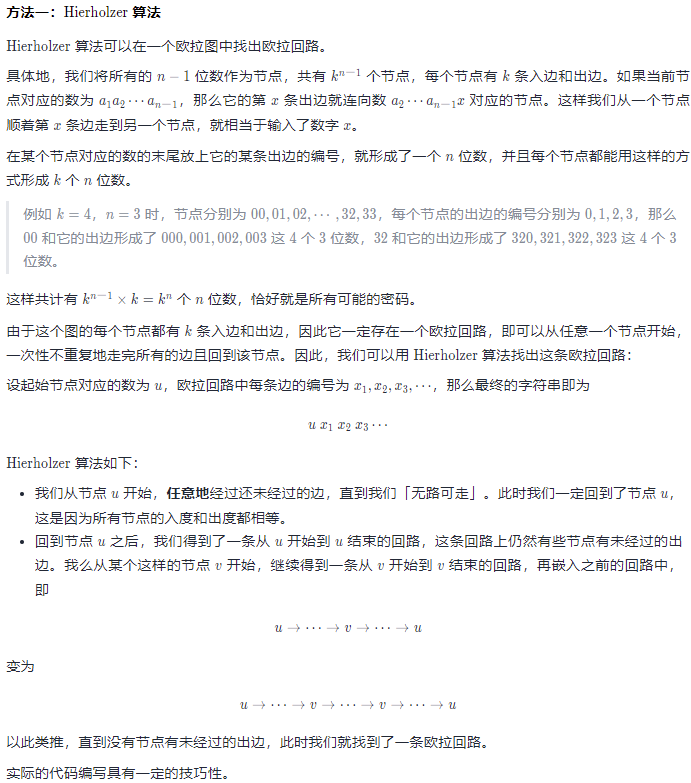
\includegraphics[width=.9\linewidth]{./pic/crackingSafe.png}

由于这个图的每个节点都有 kk 条入边和出边,因此它一定存在一个欧拉回路,即可以从任意一个节点开始,一次性不重复地走完所有的边且回到该节点。因此,我们可以用 \text{Hierholzer}Hierholzer 算法找出这条欧拉回路:
​
我们从节点 uu 开始,任意地经过还未经过的边,直到我们「无路可走」。此时我们一定回到了节点 uu,这是因为所有节点的入度和出度都相等。

回到节点 uu 之后,我们得到了一条从 uu 开始到 uu 结束的回路,这条回路上仍然有些节点有未经过的出边。我么从某个这样的节点 vv 开始,继续得到一条从 vv 开始到 vv 结束的回路,再嵌入之前的回路中,即

u→⋯→v→⋯→u

变为

u→⋯→v→⋯→v→⋯→u

\begin{minted}[fontsize=\scriptsize,linenos=false]{csharp}
Set<Integer> seen = new HashSet<Integer>();
StringBuffer ans = new StringBuffer();
int highest;
int k;
public String crackSafe(int n, int k) {
    highest = (int) Math.pow(10, n - 1);
    this.k = k;
    dfs(0);
    for (int i = 1; i < n; i++) 
        ans.append('0');
    return ans.toString();
}
public void dfs(int node) {
    for (int x = 0; x < k; ++x) {
        int nei = node * 10 + x;
        if (!seen.contains(nei)) {
            seen.add(nei);
            dfs(nei % highest);
            ans.append(x); // 这里dfs之后才添加的顺序狠重要
        }
    }
}
\end{minted}
\item 解题思路与分析
\label{sec-12-4-1-2}

密码共有n位,每一个位可以有k个数字,总共不同的密码总数就有k的n次方个。思路是先从n位都是0的密码开始,取出钥匙串的最后 n-1 个数字,然后在后面依次添加其他数字,用一个 HashSet 来记录所有遍历过的密码,这样如果不在集合中,说明是一个新密码,而生成这个新密码也只是多加了一个数字,能保证钥匙串最短,这是一种贪婪的解法,相当的巧妙

\begin{minted}[fontsize=\scriptsize,linenos=false]{csharp}
public String crackSafe(int n, int k) {
    int N = (int)Math.pow(k, n); // 第个位有k种取值,总共有k^n种不同的状态
    String s = "0".repeat(n);
    Set<String> ss = new HashSet<>(List.of(s.toString()));
    for (int i = 0; i < N; i++) {
        String pre = s.substring(s.length() - (n-1));
        // for (int j = 0; j < k; j++) { // 这里需要倒回来
        for (int j = k-1; j >= 0; j--) { 
            String cur = pre + String.valueOf(j);
            if (!ss.contains(cur)) {
                ss.add(cur);
                s += "" + j;
                break;
            }
        }
    }
    return s;
}
\end{minted}

其实在初看Hierholzer算法时,很容易产生一种想法,就是我只需要从一个节点遍历,每次把它经历的边加入到结果字符串中,当回到初始点时就完成一圈,但是这样实现的话有个明显的问题,就是每个节点都有自环,如果你遍历到某个节点时,直接跳过了自环,去了其他节点,那就失去了回来的机会(想想回家的时候虽然你可以绕小路,也可以走大路,但只要你走大路到家了,就不可能再回到学校从小路回家)。实际上不只是自环,还有可能有其他边没循环到,因为回到自身路径过多,很多边都可能没有利用。

而官方题解中的dfs巧妙的解决了这个问题,实际上它不只是沿着边走,而是把每一个边的组合都遍历到,并且在遍历之后才将有用的节点嵌套到字符串中。在dfs中,每次循环时,并不是直接将该边加入到字符串中,而是在循环之后,实际上可以想成是用了一个栈,反序的将合法的序列弹出了(dfs中的每次循环都会探索一个节点能到达的结尾在哪里,并且因为记录了每一条删除的边,所以其并不会走之前走过的路,找到结尾后回溯到还有边可走的点,继续向下走,而在该点所有可行边都已回溯完毕后,才到他自己,所以其实所有边都已经到达,并且顺序是逆序)。所以在主函数中,在得到整个序列后,才将初始的节点放入字符串末尾(如果正序的话,你应该将它放到字符串的开头)。

\item 解题思路与分析: 递归写法
\label{sec-12-4-1-3}

来看同一种解法的递归写法,思路和迭代的写法一模一样,写法略有不同而已

\begin{minted}[fontsize=\scriptsize,linenos=false]{csharp}
public String crackSafe(int n, int k) {
    N = (int)Math.pow(k, n); // 第个位有k种取值,总共有k^n种不同的状态
    s = "0".repeat(n);
    Set<String> ss = new HashSet<>(List.of(s.toString()));
    dfs(ss, n, k);
    return s;
}
String s;
int N;
void dfs(Set<String> ss, int n, int k) {
    if (ss.size() == N) return; 
    String pre = s.substring(s.length() - (n-1));
    for (int i = k-1; i >= 0; i--) {
        String cur = pre + i;
        if (ss.contains(cur)) continue;
        s += "" + i;
        ss.add(cur);
        dfs(ss, n, k);
    }
}
\end{minted}
\end{enumerate}
\subsection{332. Reconstruct Itinerary - Medium 欧拉回路 Hierholzer 算法}
\label{sec-12-4-2}
You are given a list of airline tickets where tickets[i] = [fromi, toi] represent the departure and the arrival airports of one flight. Reconstruct the itinerary in order and return it.

All of the tickets belong to a man who departs from "JFK", thus, the itinerary must begin with "JFK". If there are multiple valid itineraries, you should return the itinerary that has the smallest lexical order when read as a single string.

For example, the itinerary ["JFK", "LGA"] has a smaller lexical order than ["JFK", "LGB"].
You may assume all tickets form at least one valid itinerary. You must use all the tickets once and only once.
\begin{enumerate}
\item 解题思路与分析
\label{sec-12-4-2-1}

我们化简本题题意:给定一个 nn 个点 mm 条边的图,要求从指定的顶点出发,经过所有的边恰好一次(可以理解为给定起点的「一笔画」问题),使得路径的字典序最小。

\begin{itemize}
\item 这种「一笔画」问题与欧拉图或者半欧拉图有着紧密的联系,下面给出定义:
\begin{itemize}
\item 通过图中所有边恰好一次且行遍所有顶点的通路称为 \textbf{欧拉通路} 。
\item 通过图中所有边恰好一次且行遍所有顶点的回路称为 \textbf{欧拉回路} 。
\item 具有欧拉回路的无向图称为 \textbf{欧拉图} 。
\item 具有欧拉通路但不具有欧拉回路的无向图称为 \textbf{半欧拉图} 。
\end{itemize}
\end{itemize}

因为本题保证至少存在一种合理的路径,也就告诉了我们,这张图是一个欧拉图或者半欧拉图。我们只需要输出这条欧拉通路的路径即可。

\begin{itemize}
\item 如果没有保证至少存在一种合理的路径,我们需要判别这张图是否是欧拉图或者半欧拉图,具体地:
\begin{itemize}
\item 对于无向图 G,G 是欧拉图当且仅当 G 是连通的且没有奇度顶点。
\item 对于无向图 G,G 是半欧拉图当且仅当 G 是连通的且 G 中恰有 2 个奇度顶点。
\item 对于有向图 G,G 是欧拉图当且仅当 G 的所有顶点属于同一个强连通分量且每个顶点的入度和出度相同。
\item 对于有向图 G,G 是半欧拉图当且仅当 G 的所有顶点属于同一个强连通分量且
\begin{itemize}
\item 恰有一个顶点的出度与入度差为 1;
\item 恰有一个顶点的入度与出度差为 1;
\item 所有其他顶点的入度和出度相同。
\end{itemize}
\end{itemize}
\end{itemize}
\item 解题思路与分析: Hierholzer 算法
\label{sec-12-4-2-2}
\begin{itemize}
\item Hierholzer 算法用于在连通图中寻找欧拉路径,其流程如下:
\begin{itemize}
\item 从起点出发,进行深度优先搜索。
\item 每次沿着某条边从某个顶点移动到另外一个顶点的时候,都需要删除这条边。
\item 如果没有可移动的路径,则将所在节点加入到栈中,并返回。
\end{itemize}
\end{itemize}

当我们顺序地考虑该问题时,我们也许很难解决该问题,因为我们无法判断当前节点的哪一个分支是「死胡同」分支。

不妨倒过来思考。我们注意到只有那个入度与出度差为 11 的节点会导致死胡同。而该节点必然是最后一个遍历到的节点。我们可以改变入栈的规则,当我们遍历完一个节点所连的所有节点后,我们才将该节点入栈(即逆序入栈)。

对于当前节点而言,从它的每一个非「死胡同」分支出发进行深度优先搜索,都将会搜回到当前节点。而从它的「死胡同」分支出发进行深度优先搜索将不会搜回到当前节点。也就是说当前节点的死胡同分支将会优先于其他非「死胡同」分支入栈。

这样就能保证我们可以「一笔画」地走完所有边,最终的栈中逆序地保存了「一笔画」的结果。我们只要将栈中的内容反转,即可得到答案。

\begin{minted}[fontsize=\scriptsize,linenos=false]{csharp}
public List<String> findItinerary(List<List<String>> tickets) {
    for (List<String> t : tickets) 
        m.computeIfAbsent(t.get(0), z -> new PriorityQueue<>()).offer(t.get(1));
    List<String> ans = new ArrayList<>();
    dfs("JFK", ans);
    Collections.reverse(ans);
    return ans;
}
Map<String, PriorityQueue<String>> m = new HashMap<>(); // PriorityQueue已经默认是最小字典序,免去了排序的操作
void dfs(String s, List<String> l) {
    Queue<String> next = m.get(s);
    while (next != null && next.size() > 0)
        dfs(next.poll(), l);
    l.add(s);
}
\end{minted}
\item 解题思路与分析: Hierholzer 算法,同上,但用LinkedList可以从头插入
\label{sec-12-4-2-3}

Greedy DFS, building the route backwards when retreating.

这题其实和我之前用 DFS 处理 topological sort 的代码非常像,主要区别在于存 graph 的方式不同,这里是一个 String 直接连着对应的 next nodes,而且形式是 min heap:

\begin{itemize}
\item 原题给的是 edges,所以图是自己用 hashmap 建的。
\begin{itemize}
\item min heap 可以自动保证先访问 lexicographical order 较小的;
\item 同时 poll 出来的 node 自动删除,免去了用 List 的话要先 collections.sort 再 remove 的麻烦。
\item 这种以 “edge” 为重心的算法多靠 heap,比如 dijkstra.
\end{itemize}
\end{itemize}

Hierholzer算法的精髓是当每次访问一条边的时候,删除这条边,当遍历完一个节点所连的所有节点后,才将该节点入栈,最后将栈中的节点反转,即可得到欧拉路径

\begin{minted}[fontsize=\scriptsize,linenos=false]{csharp}
public List<String> findItinerary(String[][] tickets) {
    LinkedList<String> ans = new LinkedList<>();
    for (String[] t : tickets)
        map.computeIfAbsent(t.get(0), z -> new ArrayList<>()).offer(t.get(1));
    dfs("JFK", ans);
    return new ArrayList<String>(ans); // LinkedList最后需要转换成ArrayList
}
HashMap<String, PriorityQueue<String>> map = new HashMap<>();
void dfs(String airport, LinkedList<String> list) {
    while (map.containsKey(airport) && !map.get(airport).isEmpty())
        dfs(map.get(airport).poll(), l);
    list.offerFirst(airport); // LinkedList可以这么写
}
\end{minted}
\item 解题思路与分析: Fleury算法: leetcode还有一道割点割边的题,找出来 todo
\label{sec-12-4-2-4}
\begin{itemize}
\item 一些概念:
\begin{itemize}
\item 割点: 在一个无向图中,如果有一个顶点集合,删除这个顶点集合以及这个集合中所有顶点相关联的边以后,图的连通分量增多,就称这个点集为割点集合,如果某个割点集合只含有一个顶点 X(也即\{X\}是一个割点集合),那么X称为一个割点
\item 割边: 在一个无向图中,如果有一个边集合,删除这个边集合以后,图的连通分量增多,就称这个边集为割边集合,如果某个割边集合只含有一条边 X(也即\{X\}是一个边集合),那么X称为一个割边,也叫做桥
\end{itemize}

\item 步骤
\begin{itemize}
\item 1.如果要找欧拉回路,可以从任意点开始,如果要找欧拉路径,需要从有着奇数度的两个及顶点中的一个开始,如果有奇数度顶点的话
\item 2.选择当前点相连的边,确保删除该边,不会将欧拉图分成两个不同的联通分量
\item 3.将该边加入到路径中,并将该边从欧拉图中删除,如果当前的选择有一个桥与非桥的边时候,优先选非桥的边,不到万不得已,不选桥
\item 4.持续该过程直到路径收集完成
\end{itemize}

\item 分析: 上面的步骤中,选桥边与非桥边的时候,如何判断当前的边是否是桥,这个过程很关键,大体的思路是:
\begin{itemize}
\item 从当前节点u出发,计数,哪些顶点可以通过u可达,直接可达和间接可达均可以,记为cnt1
\item 移除掉u-v这条边
\item 从当前节点v出发,,哪些顶点可以通过v可达,直接可达和间接可达均可以,记为cnt2
\item 恢复u-v这条边
\item 返回cnt1与cnt2的大小,如果cnt2要比cnt1小,说明移除u-v这条边,从v可达的顶点数量减少,产生了额外的联通分量,此时返回falase,说明这条边是桥,反之返回true

\begin{minted}[fontsize=\scriptsize,linenos=false]{csharp}
public List<String> findItinerary(List<List<String>> tickets) { // 这个算法还比较陌生
    for (List<String> t : tickets) 
        adj.computeIfAbsent(t.get(0), z -> new ArrayList<>()).add(t.get(1));
    for (List<String> values : adj.values()) Collections.sort(values);
    String u = "JFK";
    ans.add(u);
    fleuryProcess(u);
    return ans;
}
Map<String, List<String>> adj = new HashMap<>();
List<String> ans = new ArrayList<>();
private void fleuryProcess(String u) {
    if (!adj.containsKey(u)) return ;
    for (int i = 0; i < adj.get(u).size(); i++) {
        String v = adj.get(u).get(i);
        if (isValidNextEdge(u, v)) {
            ans.add(v);
            adj.get(u).remove(v);
            fleuryProcess(v);
        }
    }
}
private boolean isValidNextEdge(String u, String v) { // 判断是否是割边:
    if (adj.get(u).size() == 1) return true;
    // boolean[] visited = new boolean[adj.get(u).size()];
    Map<String, Boolean> vis = new HashMap<>(); // vis: visited
    int cnt1 = dfs(u, vis);
    adj.get(u).remove(v);
    vis.clear(); // vis = new HashMap<>();
    int cnt2 = dfs(v, vis);
    adj.get(u).add(0, v);
    return cnt1 <= cnt2; // 如果cnt2要比cnt1小,说明移除u-v这条边,从v可达的顶点数量减少,产生了额外的联通分量,此时返回 falase, 说明这条边是桥; 反之返回 true 
}
private int dfs(String u, Map<String, Boolean> vis) {
    vis.put(u, true);
    int cnt = 1;
    if (adj.containsKey(u)) 
        for (String v : adj.get(u)) 
            if (vis.get(v) == null || (vis.get(v) != null && !vis.get(v))) 
                cnt += dfs(v, vis);
    return cnt;
}
\end{minted}
\end{itemize}
\end{itemize}
\end{enumerate}
\subsection{2097. Valid Arrangement of Pairs - Hard 欧拉回路}
\label{sec-12-4-3}
You are given a 0-indexed 2D integer array pairs where pairs[i] = [starti, endi]. An arrangement of pairs is valid if for every index i where 1 <= i < pairs.length, we have endi-1 == starti.

Return any valid arrangement of pairs.

Note: The inputs will be generated such that there exists a valid arrangement of pairs.
\begin{enumerate}
\item 解题思路与分析
\label{sec-12-4-3-1}
\begin{minted}[fontsize=\scriptsize,linenos=false]{csharp}
// One thing different is that we need to find the start point. it is obvious that if indegree is larger than 0, that is the start point.
public int[][] validArrangement(int[][] pairs) { 
    Map<Integer, Integer> ins = new HashMap<>();
    for (int [] p : pairs) {
        adj.computeIfAbsent(p[0], z -> new ArrayList<>()).add(p[1]);
        ins.put(p[0], ins.getOrDefault(p[0], 0) + 1);
        ins.put(p[1], ins.getOrDefault(p[1], 0) - 1);
    }
    int bgn = -1;
    for (Integer key : ins.keySet()) 
        if (ins.get(key) > 0) {
            bgn = key;
            break;
        }
    if (bgn == -1) bgn = pairs[0][0]; // 如果没有,就可以随便从某一个点开始?
    dfs(bgn);
    int n = pairs.length;
    int [][] ans = new int [n][];
    for (int i = n-1; i >= 0; i--) // 所以这里添加答案,也需要反序回正
        ans[n-1-i] = ll.get(i);
    return ans;
}
Map<Integer, List<Integer>> adj = new HashMap<>();
List<int []> ll = new ArrayList<>();
void dfs(int node) {
    while (adj.get(node) != null && adj.get(node).size() > 0) {
        List<Integer> nextNodesCandi = adj.get(node);
        int next = nextNodesCandi.get(nextNodesCandi.size()-1); // 从后往前遍历,方便从后往前删除已经遍历过的节点
        adj.get(node).remove(nextNodesCandi.size()-1);
        dfs(next);
        ll.add(new int [] {node, next}); // 这里的顺序是倒着加的,dfs完接下来的答案、之后再加的
    }
}
\end{minted}
\item 解题思路与分析: todo: 这个答案没有看懂
\label{sec-12-4-3-2}
\begin{minted}[fontsize=\scriptsize,linenos=false]{csharp}
// In a word, this solution is to first determine whether the target is an Euler circuit or an Euler path, then solve it.
public int[][] validArrangement(int[][] pairs) {
    int n = pairs.length;
    Map<Integer, Integer> outdegree = new HashMap<>();
    Map<Integer, Deque<Integer>> out = new HashMap<>();
    for (int[] pair : pairs) {
        outdegree.put(pair[0], outdegree.getOrDefault(pair[0], 0) + 1);
        outdegree.put(pair[1], outdegree.getOrDefault(pair[1], 0) - 1);
    }
    int[][] ans = new int[n][2];
    for (int i = 0; i < n; i++) 
        Arrays.fill(ans[i], -1);
    for (Map.Entry<Integer, Integer> en : map.entrySet()) { // 试图寻找起始和结束的位置
        if (en.getValue() == 1) ans[0][0] = en.getKey();
        if (en.getValue() == -1) ans[n-1][1] = en.getKey();
    }
    if (ans[0][0] == -1) { // 这里为什么就可以从第一个往后搜、从两边往中间搜呢?
        ans[0][0] = pairs[0][0];
        ans[n-1][1] = pairs[0][0];
    }
    for (int[] p : pairs) {
        out.computeIfAbsent(p[0], z -> new ArrayDeque<>()).offerLast(p[1]);
        // out.computeIfAbsent(p[0], k -> new ArrayDeque<>());
        out.computeIfAbsent(p[1], k -> new ArrayDeque<>()); // 需要加上
        // out.get(p[0]).offerLast(p[1]);
    }
    int i = 0, j = n-1;
    while (i < j) { // 没看明白这中间在是做什么???
        int from = ans[i][0];
        Deque<Integer> toList = out.get(from); // 这里是个栈, 上面如果不加上,这里会是null
        if (toList.size() == 0) {
            i--;
            ans[j][0] = ans[i][0];
            j--;
            ans[j][1] = ans[j + 1][0];
        } else {
            ans[i++][1] = toList.pollLast();
            // ans[i++][1] = toList.removeLast();
            ans[i][0] = ans[i - 1][1];
        }
    }
    return ans;
}
\end{minted}
\end{enumerate}

\subsection{1591. Strange Printer II - Hard}
\label{sec-12-4-4}
There is a strange printer with the following two special requirements:

On each turn, the printer will print a solid rectangular pattern of a single color on the grid. This will cover up the existing colors in the rectangle.
Once the printer has used a color for the above operation, the same color cannot be used again.
You are given a m x n matrix targetGrid, where targetGrid[row][col] is the color in the position (row, col) of the grid.

Return true if it is possible to print the matrix targetGrid, otherwise, return false.

\begin{enumerate}
\item 解题思路与分析: 邻接有向图 + 拓扑排序
\label{sec-12-4-4-1}

这道题可以认为是在研究:是否有一种颜色序列,按照这个序列进行染色,最终矩阵就会呈现输入的状态。

矩形上的某一个像素点,可能会先后经历多次染色。比如先染红,再染绿,再染黄,最后染蓝,最后呈现出的就是蓝色。

我们知道这个像素现在是蓝色;

而它在红色/绿色/黄色矩形范围内,说明这个像素曾经红过/绿过/黄过。

此时我们可以提炼出信息:假定先染的优先于后染的,那么红色优于蓝色,绿色优于蓝色,黄色优于蓝色。

(红绿黄之间的顺序未定)。

题中指出,颜色最多有 6060 种,我们可以建立一个有向图,图中的结点就是这 6060 个颜色 1$\sim$ 601∼60 。

按照刚才的方法找出所有的有向边,进行拓扑排序即可判断出结果。

\begin{minted}[fontsize=\scriptsize,linenos=false]{csharp}
public boolean isPrintable(int[][] a) { 
    int m = a.length, n = a[0].length, max = Math.max(m, n);
    for (int i = 0; i < m; i++)
        max = Math.max(max, Arrays.stream(a[i]).max().getAsInt());
    int N = max + 1;
    int [] up = new int [N], down = new int [N], left = new int [N], right = new int [N];
    Arrays.fill(up, m);
    Arrays.fill(left, n);
    Arrays.fill(down, -1);
    Arrays.fill(right, -1);
    for (int i = 0; i < m; i++) // 界定每一种着色的上下左右边界,以便接下来排序
        for (int j = 0; j < n; j++) {
            int k = a[i][j];
            up[k] = Math.min(up[k], i);
            down[k] = Math.max(down[k], i);
            left[k] = Math.min(left[k], j);
            right[k] = Math.max(right[k], j);
        }
    // 根据每种着色的界定范围,建立拓扑排序:这后半部分还有点儿不熟练
    // 当前位置颜色 cur 在某个矩阵 k 中但是不为矩阵 k 的颜色时,建立从 k 到 cur 的边,cur 可以存在于多个矩阵中
    boolean [][] nei = new boolean [N][N];  // neighbours
    List<Integer>[] adj = new ArrayList[N]; // 邻接有向图:按照染色的先后顺序
    int [] ins = new int [N];
    for (int i = 0; i < N; i++) adj[i] = new ArrayList<>();
    for (int i = 0; i < m; i++)
        for (int j = 0; j < n; j++) {
            int cur = a[i][j]; // 当前格的最终打印着色
            for (int k = 1; k < N; k++) { // 遍历所有的着色:暴搜当前着色cur是否会在某种着色k之后染色
                if (k == cur) continue;
                if (i >= up[k] && i <= down[k] && j >= left[k] && j <= right[k])  // 现着色cur完全处于先前染色k的内部,所以cur是后着色
                    // if (!nei[cur][k]) { // BUG: 是有向图:这里顺序很重要,先染色 是否 与后染色相连/相前后
                    if (!nei[k][cur]) {    // k 先染后, cur 后染色
                        adj[k].add(cur);
                        ins[cur]++;
                        nei[k][cur] = true;
                    }
            }
        }
    List<Integer> l = new ArrayList<>();
    while (true) { // 寻找入度为 0 的颜色点,减小该点连结的点的入度,直到所有点的入度都为 0
        int i;
        for (i = 1; i < N; i++) 
            if (ins[i] == 0) {
                l.add(i);
                for (int v : adj[i]) ins[v]--;
                ins[i] = -1;
                break;
            }
        if (i == N) break;
    }
    return l.size() == max; // 按照拓扑排序,这所有的染色都可以有序地染出来,那么合法
}
\end{minted}
\item 解题思路与分析: topological sort
\label{sec-12-4-4-2}
\begin{minted}[fontsize=\scriptsize,linenos=false]{csharp}
public boolean isPrintable(int[][] a) { 
    int m = a.length, n = a[0].length;
    Set<Integer> col = new HashSet<>();
    for (int i = 0; i < m; i++) 
        for (int j = 0; j < n; j++)
            col.add(a[i][j]);
    for (Integer c : col) {
        int fi = -1, fj = Integer.MAX_VALUE, li = -1, lj = -1;  // f: first, f row, f col, l: last, l row, l col
        for (int i = 0; i < m; i++)
            for (int j = 0; j < n; j++)
                if (a[i][j] == c) {
                    if (fi == -1) fi = i; // 只记最早出现的第一次
                    fj = Math.min(fj, j);
                    li = i;
                    lj = Math.max(lj, j);
                }
        for (int i = fi; i <= li; i++) 
            for (int j = fj; j <= lj; j++) 
                if (a[i][j] != c) // a[i][j]是会在当前染色c之后染色的
                    adj.computeIfAbsent(c, z -> new HashSet<>()).add(a[i][j]);
    }
    Set<Integer> vis = new HashSet<>(); // visiting: 只保证先染的着色不会在后染的着色里再次出现
    for (Integer c : col) 
        if (!topologicalSort(vis, c)) return false;
    return true;
}
Map<Integer, Set<Integer>> adj = new HashMap<>(); // 在key之后染色的着色集合
private boolean topologicalSort(Set<Integer> vis, int c) { // 这种写法好陌生
    if (vis.contains(c)) return false;
    vis.add(c);
    for (Integer nei : adj.getOrDefault(c, Collections.emptySet()))
        if (!topologicalSort(vis, nei)) return false;
    vis.remove(c);
    return true;
}
\end{minted}
\end{enumerate}


\section{双端队列BFS}
\label{sec-12-5}
\subsection{1368. Minimum Cost to Make at Least One Valid Path in a Grid - Hard}
\label{sec-12-5-1}
Given a m x n grid. Each cell of the grid has a sign pointing to the next cell you should visit if you are currently in this cell. The sign of grid[i][j] can be:
1 which means go to the cell to the right. (i.e go from grid[i][j] to grid[i][j + 1])
2 which means go to the cell to the left. (i.e go from grid[i][j] to grid[i][j - 1])
3 which means go to the lower cell. (i.e go from grid[i][j] to grid[i + 1][j])
4 which means go to the upper cell. (i.e go from grid[i][j] to grid[i - 1][j])
Notice that there could be some invalid signs on the cells of the grid which points outside the grid.

You will initially start at the upper left cell (0,0). A valid path in the grid is a path which starts from the upper left cell (0,0) and ends at the bottom-right cell (m - 1, n - 1) following the signs on the grid. The valid path doesn't have to be the shortest.

You can modify the sign on a cell with cost = 1. You can modify the sign on a cell one time only.

Return the minimum cost to make the grid have at least one valid path.
\begin{enumerate}
\item 解题思路与分析: 0-1广度优先搜索(最优解法)
\label{sec-12-5-1-1}

这道题其实是个经典的双端队列BFS。将每个格子看成是图的顶点,相邻格子是有边相连接的。如果从顶点(x, y)到(u, v)的实际方向和矩阵在(x, y)所表示的方向相同,则令这条边的边权为0,否则令其边权为1。原题相当于在问,在此图中,从起点到终点的最短路长度是多少。由于边权只有0和1两种,所以可以用双端队列BFS来做。每次拓展的时候,如果是沿着边权0的边走的,则插入队头,否则插入队尾。从队列里取元素的时候永远都从队头取。然后用堆优化的Dijkstra算法模板来写即可。时空复杂度O(mn)。

0-1 广度优先搜索的实现其实与 Dijkstra 算法非常相似。在 Dijkstra 算法中,我们用优先队列保证了距离的单调递增性。而在 0-1 广度优先搜索中,实际上任意时刻队列中的节点与源点的距离均为 dd 或 d + 1d+1(其中 dd 为某一非负整数),并且所有与源点距离为 dd 的节点都出现在队首附近,所有与源点距离为 d + 1d+1 的节点都出现在队尾附近。因此,我们只要使用双端队列,对于边权为 00 和 11 的两种情况分别将对应节点添加至队首和队尾,就保证了距离的单调递增性。

\begin{minted}[fontsize=\scriptsize,linenos=false]{csharp}
public int minCost(int[][] g) {
    int m = g.length, n = g[0].length;
    int [][] d = new int [m][n]; // dist to [0, 0]
    for (int i = 0; i < m; i++) 
        Arrays.fill(d[i], Integer.MAX_VALUE);
    d[0][0] = 0;
    int [][] dirs = {{0, 0}, {0, 1}, {0, -1}, {1, 0}, {-1, 0}}; // [0, 1, 2, 3, 4]
    boolean [][] vis = new boolean [m][n];
    ArrayDeque<Integer> q = new ArrayDeque<>();
    q.offerFirst(0);
    while (!q.isEmpty()) {
        int idx = q.pollFirst();
        int i = idx / n, j = idx % n;
        if (vis[i][j]) continue;
        if (i == m-1 && j == n-1) return d[i][j];
        vis[i][j] = true;
        for (int k = 1; k < 5; k++) {
            int x = i + dirs[k][0], y = j + dirs[k][1];
            if (x < 0 || x >= m || y < 0 || y >= n) continue;
            int cost = k == g[i][j] ? 0 : 1;
            if (!vis[x][y] && d[x][y] > d[i][j] + cost) {
                d[x][y] = d[i][j] + cost;
                if (cost == 0) q.offerFirst(x * n + y);
                else q.offerLast(x * n + y);
            }
        }
    }
    return -1;
}
\end{minted}
\item 解题思路与分析: 最短路径问题总结 BFS
\label{sec-12-5-1-2}
\begin{enumerate}
\item 题目分析
\label{sec-12-5-1-2-1}
\begin{itemize}
\item 虽然题目的描述中写了有效路径不需要是最短路径,但其实这道题目还是一个最短路径问题,只不过要求的最短距离并不是在网格中行走的距离,而是改变方向的次数。
\item 所谓最短路径问题,就是对于图 G(V,E)G(V,E),寻找从 u$\in$ Vu∈V 到 v$\in$ Vv∈V 的最短距离。最短路径的算法有很多,包括 Dijkstra,Floyd,Bellman-Ford,SPFA 等。
\end{itemize}

\includegraphics[width=.9\linewidth]{./pic/1368.png}

对于 BFS,相信大家一定都很熟悉了。与 DFS 相比,BFS 的特点是按层遍历,从而可以保证首先找到最优解(最少步数、最小深度)。从这个意义上讲,BFS 解决的其实也是最短路径问题。这一问题对应的图 GG 包含的所有顶点即为状态空间,而每一个可能的状态转移都代表了一条边。

比如,在经典的迷宫问题中,每一个状态 (x,y)(x,y) 代表了一个顶点,而一个无障碍格子与其相邻的无障碍格子之间则存在一条无向边。

那么,这个图 GG 和一般的图相比,有什么特点呢?

关键就在于边的权值。在 BFS 问题中,所有边的权值均为 1!因为我们每一次从一个状态转移到一个新的状态,就多走了一步。正因为边权值均为 1,我们用一个队列记录所有状态,前面的状态对应的总权值一定小于后面的状态,所以我们就可以在 O(1)O(1) 的时间内实现找到最小节点并将其移除的操作(只要取队头,然后出队就可以了),从而寻找最短路径的时间复杂度就减小到了 O(V+E)O(V+E)。

但普通的 BFS 算法,在本题中并不适用,因为存在权值为 0 的边!如果从一个格子到另一个格子,不需要修改格子上的标记,那么这一步移动的权值就为 0。如果我们还沿用普通 BFS 的做法,就无法保证队头元素一定是当前具有最小权值的节点。

怎么办呢?简单粗暴的做法是:允许多次扩展同一个点。只要当前边能够更新节点的权值,就将节点再次入队。

\begin{minted}[fontsize=\scriptsize,linenos=false]{csharp}
public int minCost(int[][] g) {
    int [][] dirs = {{0, 0}, {0, 1}, {0, -1}, {1, 0}, {-1, 0}}; 
    int m = g.length, n = g[0].length;
    int [][] d = new int [m][n]; // dist to [0, 0]
    for (int i = 0; i < m; i++) 
        Arrays.fill(d[i], Integer.MAX_VALUE);
    d[0][0] = 0;
    Queue<int []> q = new LinkedList<>();
    q.offer(new int [] {0, 0});
    while (!q.isEmpty()) {
        int [] cur = q.poll();
        int i = cur[0], j = cur[1];
        for (int k = 1; k < 5; k++) {
            int x = i + dirs[k][0], y = j + dirs[k][1];
            if (x < 0 || x >= m || y < 0 || y >= n) continue;
            int newDist = d[i][j] + (k == g[i][j] ? 0 : 1);
            if (newDist < d[x][y]) {
                d[x][y] = newDist;
                q.offer(new int [] {x, y});
            }
        }
    }
    return d[m-1][n-1];
}
\end{minted}
\end{enumerate}
\item 解题思路与分析: SPFA
\label{sec-12-5-1-3}
如果一个节点已经在队列中,其实就没有必要将其再次入队了。这是 SPFA 算法的基本思想。可以看到,与上面的BFS 方法相比,就是增加了一个 in 数组来判断当前节点是否已经在队列中。

SPFA 算法是一个十分依赖于数据的算法。在特定的数据下,SPFA 会退化为 Bellman-Ford,时间复杂度为 O(V$\cdot$ E)O(V⋅E)。一般的编程竞赛中,涉及到最短路径的题目,都会有专门卡SPFA的数据,所以一般情况下还是使用 Dijkstra 算法。本题的测试数据相对较弱,BFS 和 SPFA 都可以顺利通过,甚至 SPFA 的运行时间还要长于 BFS(修改 in 数组状态带来了额外的开销)。

SPFA 的好处是可以判断负环。我们可以用一个数组记录每个顶点的入队次数,如果有顶点的入队次数超过了 VV 次,则代表图中存在负环。

\begin{minted}[fontsize=\scriptsize,linenos=false]{csharp}
public int minCost(int[][] g) {
    int [][] dirs = {{0, 0}, {0, 1}, {0, -1}, {1, 0}, {-1, 0}}; 
    int m = g.length, n = g[0].length;
    int [][] d = new int [m][n]; 
    for (int i = 0; i < m; i++) 
        Arrays.fill(d[i], Integer.MAX_VALUE);
    d[0][0] = 0;
    boolean [][] in = new boolean [m][n];
    Queue<int []> q = new LinkedList<>();
    q.offer(new int [] {0, 0});
    in[0][0] = true;
    while (!q.isEmpty()) {
        int [] cur = q.poll();
        int i = cur[0], j = cur[1];
        in[i][j] = false;
        for (int k = 1; k < 5; k++) {
            int x = i + dirs[k][0], y = j + dirs[k][1];
            if (x < 0 || x >= m || y < 0 || y >= n) continue;
            int newDist = d[i][j] + (k == g[i][j] ? 0 : 1);
            if (newDist < d[x][y]) {
                d[x][y] = newDist;
                if (!in[x][y]) {
                    q.offer(new int [] {x, y});
                    in[x][y] = true;
                }
            }
        }
    }
    return d[m-1][n-1];
}
\end{minted}
\item 解题思路与分析
\label{sec-12-5-1-4}
\end{enumerate}

\subsection{126. Word Ladder II - Hard BFS}
\label{sec-12-5-2}
A transformation sequence from word beginWord to word endWord using a dictionary wordList is a sequence of words beginWord -> s1 -> s2 -> \ldots{} -> sk such that:

Every adjacent pair of words differs by a single letter.
Every si for 1 <= i <= k is in wordList. Note that beginWord does not need to be in wordList.
sk == endWord
Given two words, beginWord and endWord, and a dictionary wordList, return all the shortest transformation sequences from beginWord to endWord, or an empty list if no such sequence exists. Each sequence should be returned as a list of the words [beginWord, s1, s2, \ldots{}, sk].
\begin{enumerate}
\item 解题思路与分析: 广度优先搜索
\label{sec-12-5-2-1}
\begin{itemize}
\item 官方题解:\url{https://leetcode-cn.com/problems/word-ladder-ii/solution/dan-ci-jie-long-ii-by-leetcode-solution/}

\begin{minted}[fontsize=\scriptsize,linenos=false]{csharp}
public List<List<String>> findLadders(String bgn, String end, List<String> list) { 
    Set<String> ss = new HashSet<>(list);
    if (!ss.contains(end)) return ans;
    ss.remove(bgn);
    // BFS: 第 1 步:广度优先遍历建图
    Map<String, Integer> cnt = new HashMap<>(); // 记录扩展出的单词是在第几次扩展的时候得到的,key:单词,value:在广度优先遍历的第几层
    cnt.put(bgn, 0);
    Map<String, List<String>> from = new HashMap<>(); // 记录了单词是从哪些单词扩展而来,key:单词,value:单词列表,这些单词可以变换到 key ,它们是一对多关系
    int step = 1, n = bgn.length();
    boolean found = false;
    Queue<String> q = new LinkedList<>();
    q.offer(bgn);
    while (!q.isEmpty()) {
        for (int size = q.size()-1; size >= 0; size--) {
            String cur = q.poll();
            char [] s = cur.toCharArray();
            for (int i = 0; i < n; i++) {
                char ori = s[i];
                for (char c = 'a'; c <= 'z'; c++) {
                    if (s[i] == c) continue; // 
                    s[i] = c;
                    String next = String.valueOf(s);
                    if (cnt.containsKey(next) && step == cnt.get(next)) //
                        from.get(next).add(cur);                        //
                    if (!ss.contains(next)) continue; // BUG: 还没有想明白,为什么我把这行写前面会少掉答案呢? 
                    ss.remove(next); // 如果从一个单词扩展出来的单词以前遍历过,距离一定更远,为了避免搜索到已经遍历到,且距离更远的单词,需要将它从 dict 中删除
                    q.offer(next);   // 这一层扩展出的单词进入队列
                    from.computeIfAbsent(next, z -> new ArrayList<>()).add(cur); // 记录 next Word 从 cur Word 而来
                    cnt.put(next, step);
                    if (next.equals(end)) found = true;
                }
                s[i] = ori;
            }
        }
        step++;
        if (found) break;
    }
    // 第 2 步:深度优先遍历找到所有解,从 end 恢复到 bgn ,所以每次尝试操作 path 列表的头部
    if (found) {
        Deque<String> path = new ArrayDeque<>(); 
        path.add(end);
        dfs(from, path, bgn, end);
    }
    return ans;
}
List<List<String>> ans = new ArrayList<>();
void dfs(Map<String, List<String>> from, Deque<String> path, String end, String cur) {
    if (cur.equals(end)) {
        ans.add(new ArrayList<>(path)); // 这个写法学习一下,第一次见
        return ;
    }
    for (String precursor : from.get(cur)) {
        path.offerFirst(precursor);
        dfs(from, path, end, precursor);
        path.pollFirst();
    }
}
\end{minted}
\end{itemize}
\item 解题思路与分析: 详细通俗的思路分析,多解法: DFS + BFS 双向搜索(two-end BFS)双向BFS搜索
\label{sec-12-5-2-2}
\begin{itemize}
\item \url{https://leetcode-cn.com/problems/word-ladder-ii/solution/xiang-xi-tong-su-de-si-lu-fen-xi-duo-jie-fa-by-3-3/}
\end{itemize}

这个题解和自己最初解法比较接近,需要再好好学习一下
\begin{minted}[fontsize=\scriptsize,linenos=false]{csharp}
 public List<List<String>> findLadders(String beginWord, String endWord, List<String> wordList) {
    List<List<String>> ans = new ArrayList<>();
    if (!wordList.contains(endWord)) return ans;
    // 利用 BFS 得到所有的邻居节点
    HashMap<String, ArrayList<String>> map = new HashMap<>();
    bfs(beginWord, endWord, wordList, map);
    ArrayList<String> temp = new ArrayList<String>();
    // temp 用来保存当前的路径
    temp.add(beginWord);
    findLaddersHelper(beginWord, endWord, map, temp, ans);
    return ans;
}
private void findLaddersHelper(String beginWord, String endWord, HashMap<String, ArrayList<String>> map,
                               ArrayList<String> temp, List<List<String>> ans) {
    if (beginWord.equals(endWord)) {
        ans.add(new ArrayList<String>(temp));
        return;
    }
    // 得到所有的下一个的节点
    ArrayList<String> neighbors = map.getOrDefault(beginWord, new ArrayList<String>());
    for (String neighbor : neighbors) {
        temp.add(neighbor);
        findLaddersHelper(neighbor, endWord, map, temp, ans);
        temp.remove(temp.size() - 1);
    }
}
// 利用递归实现了双向搜索
private void bfs(String beginWord, String endWord, List<String> wordList, HashMap<String, ArrayList<String>> map) {
    Set<String> set1 = new HashSet<String>();
    set1.add(beginWord);
    Set<String> set2 = new HashSet<String>();
    set2.add(endWord);
    Set<String> wordSet = new HashSet<String>(wordList);
    bfsHelper(set1, set2, wordSet, true, map);
}
// direction 为 true 代表向下扩展,false 代表向上扩展
private boolean bfsHelper(Set<String> set1, Set<String> set2, Set<String> wordSet, boolean direction,
                          HashMap<String, ArrayList<String>> map) {
    // set1 为空了,就直接结束
    // 比如下边的例子就会造成 set1 为空
    /*	"hot"
        "dog"
        ["hot","dog"]*/
    if (set1.isEmpty()) return false;
    // set1 的数量多,就反向扩展
    if (set1.size() > set2.size()) 
        return bfsHelper(set2, set1, wordSet, !direction, map);
    // 将已经访问过单词删除
    wordSet.removeAll(set1);
    wordSet.removeAll(set2);
    boolean done = false;
    // 保存新扩展得到的节点
    Set<String> set = new HashSet<String>();
    for (String str : set1) {
        // 遍历每一位
        for (int i = 0; i < str.length(); i++) {
            char[] chars = str.toCharArray();
            // 尝试所有字母
            for (char ch = 'a'; ch <= 'z'; ch++) {
                if(chars[i] == ch) continue;
                chars[i] = ch;
                String word = new String(chars);
                // 根据方向得到 map 的 key 和 val
                String key = direction ? str : word;
                String val = direction ? word : str;
                ArrayList<String> list = map.containsKey(key) ? map.get(key) : new ArrayList<String>();
                // 如果相遇了就保存结果
                if (set2.contains(word)) {
                    done = true;
                    list.add(val);
                    map.put(key, list);
                }
                // 如果还没有相遇,并且新的单词在 word 中,那么就加到 set 中
                if (!done && wordSet.contains(word)) {
                    set.add(word);
                    list.add(val);
                    map.put(key, list);
                }
            }
        }
    }
    // 一般情况下新扩展的元素会多一些,所以我们下次反方向扩展  set2
    return done || bfsHelper(set2, set, wordSet, !direction, map);
}
\end{minted}
\end{enumerate}

\section{环与入度等}
\label{sec-12-6}
\subsection{685. Redundant Connection II - Hard}
\label{sec-12-6-1}
In this problem, a rooted tree is a directed graph such that, there is exactly one node (the root) for which all other nodes are descendants of this node, plus every node has exactly one parent, except for the root node which has no parents.

The given input is a directed graph that started as a rooted tree with n nodes (with distinct values from 1 to n), with one additional directed edge added. The added edge has two different vertices chosen from 1 to n, and was not an edge that already existed.

The resulting graph is given as a 2D-array of edges. Each element of edges is a pair [ui, vi] that represents a directed edge connecting nodes ui and vi, where ui is a parent of child vi.

Return an edge that can be removed so that the resulting graph is a rooted tree of n nodes. If there are multiple answers, return the answer that occurs last in the given 2D-array.
\begin{enumerate}
\item 解题思路与分析
\label{sec-12-6-1-1}
\begin{minted}[fontsize=\scriptsize,linenos=false]{csharp}
// 对于有向图中,如果存在indegree(v) == 2的点,那么要删除的一定是这个点的某条有向边(u -> v)
//    因为题目最后保证是一个rooted tree(every node has exactly one parent),具体看第一段定义;
// 如果不存在indegree(v) == 2的点,那么直接删去最后一个造成环存在的有向边即可。
// 现在存在三种情况:
// (1)有向图中只有环。这种情况就简单将两个节点具有共同根节点的边删去就好。
// (2)有向图中没有环,但有个节点有两个父节点。这种情况就将第二次出现不同父节点的边删去就好。
// (3)有向图中既有环,而且有个节点还有两个父节点。这时就检测当除去第二次出现父节点的边后,剩余边是不是合法的,如果不合法证明应该删掉的是另一个父节点的边。
public int [] findRedundantDirectedConnection(int [][] egs) {
    Set<Integer> p = new HashSet<>();
    Map<Integer, Integer> par = new HashMap<>(); // k,v: v <-- u
    List<int []> candi = new ArrayList<>();
    for (int [] e : egs) {
        int u = e[0], v = e[1];
        p.add(u);
        p.add(v);
        if (!par.containsKey(v)) { // 对于入度为1的右端点边,记在字典里
            par.put(v, u);
            continue;
        }
        candi.add(new int [] {par.get(v), v}); // 第一次出现的边
        candi.add(new int [] {u, v});          // 第二次出现的边,答案是这两者之一
        e[1] = -1; // 先将后出现的第二条边废掉,验证答案
    }
    UnionFind uf = new UnionFind(p.size()); // 总顶点的个数
    for (int [] e : egs) {
        if (e[1] == -1) continue;   // 跳过正在验证是否为的答案后出现的第二条边
        int u = e[0]-1, v = e[1]-1; // uf 0-based
        if (!uf.union(u, v)) { // 在已经废除后出现的第二条边之后,还是出现了环,那么后出现的第二条边不是答案,第一条才是
            if (candi.isEmpty()) return e; // 不存在入度为 2 的点,直接删去最后一条造成环存在的有向边, 即当前边即可
            return candi.get(0);
        }
    }
    return candi.get(1); // 删除第二条边后,所有的存在都合法,那么就返回第二条边
}
class UnionFind {
    int[] parent;
    int[] rank;
    int size;
    public UnionFind(int size) {
        this.size = size;
        parent = new int[size];
        rank = new int[size];
        for (int i = 0; i < size; i++) parent[i] = i;
    }
    public int find(int x) {
        if (parent[x] != x) 
            parent[x] = find(parent[x]);
        return parent[x];
    }
    public boolean union(int x, int y) { 
        int xp = find(x);
        int yp = find(y);
        if (xp == yp) return false; // 已经在同一个强连通分量中
        if (rank[xp] > rank[yp]) 
            parent[yp] = xp;
        else if (rank[xp] < rank[yp]) 
            parent[xp] = yp;
        else {
            parent[yp] = xp;
            rank[xp]++;
        }
        return true;
    }
}
\end{minted}
\end{enumerate}
\section{普通BFS,但state状态狠重要}
\label{sec-12-7}
\subsection{1293. Shortest Path in a Grid with Obstacles Elimination - Hard}
\label{sec-12-7-1}
You are given an m x n integer matrix grid where each cell is either 0 (empty) or 1 (obstacle). You can move up, down, left, or right from and to an empty cell in one step.

Return the minimum number of steps to walk from the upper left corner
(0, 0) to the lower right corner (m - 1, n - 1) given that you can
eliminate at most k obstacles. If it is not possible to find such walk
return -1.
\begin{enumerate}
\item 解题思路与分析
\label{sec-12-7-1-1}
\begin{itemize}
\item 在普通的bfs中,为了避免走重复的路径,我们一般采用visited数组来记录下走过的格子,当路径遇到一个已走过的格子时,便不能再通过该点。但本题略有不同,上面说过,本题存在两种路径,因此visited数组中的状态应该包含3中状态:
\begin{itemize}
\item 0:该位置没有走过
\item 1:该位置被普通路径走过
\item 2:该路径被穿越路径走过
\end{itemize}
\item 对于以上三种状态,
\begin{itemize}
\item 当前格子为非障碍物时,普通路径可以走访问状态为0的格子,走过后,访问状态更新为1
\item 当前格子为非障碍物时,穿越路径可以走访问状态为0的格子,走过后,访问状态更新为2
\item 当前格子为非障碍物时,普通路径可以走访问状态为2的格子,走过后,访问状态更新为1
\item 当前格子为障碍物时,如果还保有穿越次数,并且该格子的访问状态为0时,所有路径可以通过此处,通过后,该路径变为穿越路径,并且当前格子访问状态更新为1(更新为2也无所谓)
\begin{minted}[fontsize=\scriptsize,linenos=false]{csharp}
public int shortestPath(int[][] a, int k) {
    int [][] dirs = {{1, 0}, {-1, 0}, {0, 1}, {0, -1}};
    int m = a.length, n = a[0].length;
    int [][] vis = new int [m][n]; 
    Deque<int []> q = new ArrayDeque<>();
    q.offerLast(new int [] {0, 0, k});
    int cnt = 0;
    while (!q.isEmpty()) {
        for (int z = q.size()-1; z >= 0; z--) {
            int [] cur = q.pollFirst();
            if (cur[0] == m-1 && cur[1] == n-1) return cnt;
            for (int [] d : dirs) {
                int i = cur[0] + d[0], j = cur[1] + d[1];
                if (i >= 0 && i < m && j >= 0 && j < n) {
// 1.当前格子为非障碍物时,普通路径可以走访问状态为 0 的格子,走过后,访问状态更新为1
// 3.当前格子为非障碍物时,普通路径可以走访问状态为 2 的格子,走过后,访问状态更新为1
                    if (a[i][j] == 0 && (vis[i][j] == 0 || vis[i][j] == 2 && cur[2] == k)) { // 当前格为非障碍物
                        if (vis[i][j] == 0) // 普通路径:可以走状态为0的格子,走过后变为1 or 2
                            // 2.当前格子为非障碍物时,穿越路径可以走访问状态为0的格子,走过后,访问状态更新为2 
                            vis[i][j] = (cur[2] == k ? 1 : 2);
                        else vis[i][j] = 1;
                        q.offerLast(new int [] {i, j, cur[2]});
                        // 4.当前格子为障碍物时,如果还保有穿越次数,并且该格子的访问状态为0时,所有路径可以通过此处,
                        //     通过后,该路径变为穿越路径,并且当前格子访问状态更新为1(更新为2也无所谓)                                
                    } else if (a[i][j] == 1 && vis[i][j] == 0 && cur[2] > 0) {
                        vis[i][j] = 2;
                        q.offerLast(new int [] {i, j, cur[2]-1});
                    }
                }
            }
        }
        cnt++;
    }
    return -1;
}
\end{minted}
\end{itemize}
\end{itemize}
\item 解题思路与分析
\label{sec-12-7-1-2}
\begin{itemize}
\item 思路是BFS。将已经移除了多少个障碍物加进状态,然后做隐式图搜索即可。代码如下:
\begin{minted}[fontsize=\scriptsize,linenos=false]{csharp}
public int shortestPath(int[][] a, int k) { // 这个思路极为简洁,但速度跟上一个方法比,会慢很多
    if (a.length <= 1 && a[0].length <= 1) return 0;
    int [][] dirs = {{1, 0}, {-1, 0}, {0, 1}, {0, -1}};
    int m = a.length, n = a[0].length;
    boolean [][][] vis = new boolean [m][n][k+1];
    Deque<int []> q = new ArrayDeque<>();
    q.offerLast(new int [] {0, 0, 0}); // 前两个数代表坐标,最后一个数代表已经移除了多少个障碍物
    vis[0][0][0] = true;
    int cnt = 0;
    while (!q.isEmpty()) {
        for (int z = q.size()-1; z >= 0; z--) {
            int [] cur = q.pollFirst();
            for (int [] d : dirs) {
                int i = cur[0] + d[0], j = cur[1] + d[1], x = -1;
                if (i < 0 || i >= m || j < 0 || j >= n) continue;
                x = cur[2] + a[i][j];
                if (k >= x && !vis[i][j][x]) {
                    if (i == a.length-1 && j == a[0].length-1) return cnt+1;
                    q.offerLast(new int [] {i, j, x});
                    vis[i][j][x] = true;
                }
            }
        }
        cnt++;
    }
    return -1;
}
\end{minted}
\end{itemize}
\end{enumerate}


\section{最小生成树}
\label{sec-12-8}
\subsection{1489. Find Critical and Pseudo-Critical Edges in Minimum Spanning Tree - Hard}
\label{sec-12-8-1}
Given a weighted undirected connected graph with n vertices numbered from 0 to n - 1, and an array edges where edges[i] = [ai, bi, weighti] represents a bidirectional and weighted edge between nodes ai and bi. A minimum spanning tree (MST) is a subset of the graph's edges that connects all vertices without cycles and with the minimum possible total edge weight.

Find all the critical and pseudo-critical edges in the given graph's minimum spanning tree (MST). An MST edge whose deletion from the graph would cause the MST weight to increase is called a critical edge. On the other hand, a pseudo-critical edge is that which can appear in some MSTs but not all.

Note that you can return the indices of the edges in any order.
\begin{enumerate}
\item 解题思路与分析
\label{sec-12-8-1-1}
\begin{minted}[fontsize=\scriptsize,linenos=false]{csharp}
public List<List<Integer>> findCriticalAndPseudoCriticalEdges(int n, int[][] edges) {
    List<int []> lia = new ArrayList<>();
    for (int [] e : edges) lia.add(e);
    Collections.sort(lia, (x, y) -> x[2] - y[2]);
    List<Integer> critical = new ArrayList<>();
    List<Integer> pseudo = new ArrayList<>();
    int minCost = getCostOfMST(n, lia, null, null);
    for (int i = 0; i < edges.length; i++) {
        int [] e = edges[i];
        if (getCostOfMST(n, lia, null, e) > minCost) // 优先条件:如果已经是critical,就不用考虑后面的了
            critical.add(i);
        else if (getCostOfMST(n, lia, e, null) == minCost)
            pseudo.add(i);
    }
    return Arrays.asList(critical, pseudo);
}
int getCostOfMST(int n, List<int []> adj, int [] req, int [] avd) { // avoid 
    int ans = 0;
    DSU dsu = new DSU(n);
    if (req != null) {
        dsu.union(req[0], req[1]);
        ans += req[2];
    }
    for (int [] e : adj) {
        if (e != avd && dsu.union(e[0], e[1])) // 可以合并
            ans += e[2];
        if (dsu.getCnt() == 1)
            return ans;
    }
    return Integer.MAX_VALUE; // 无法生成合法的最小生成树
}
static class DSU {
    int [] par;
    int [] rank; // 关于rank和size的部分
    int size;
    public boolean union(int x, int y) {
        int px = find(x), py = find(y);
        if (px == py) return false;
        // if (rank[x] >= rank[y]) { // BUG
        if (rank[px] >= rank[py]) {
            par[py] = px;
            if (rank[px] == rank[py])
                ++rank[px];
            // rank[x] += rank[y]; // BUG: 这里自己写错了
        } else {
            par[px] = py;
            // rank[y] += rank[x];
        }
        --size;
        return true;
    }
    public int getCnt() {
        return size;
    }
    int find(int x) {
        // if (par[x] != x) par[x] = find(par[x]); // BUG
        while (par[x] != x) {
            par[x] = par[par[x]];
            x = par[x];
        }
        return par[x];
    }
    public DSU(int n) {
        size = n;
        par = new int [n];
        rank = new int [n];
        for (int i = 0; i < n; i++) 
            par[i] = i;
    }
}
\end{minted}
\item 解题思路与分析
\label{sec-12-8-1-2}
\begin{itemize}
\item 这是自己慢慢掰出来的,掰还第二遍的时候掰错了。。。最好是能够参考一下别人的最优解法
\end{itemize}
\begin{minted}[fontsize=\scriptsize,linenos=false]{csharp}
HashMap<Integer, int []> m = new HashMap<>(); // 这是参考以前写的
HashSet<Integer> s = new HashSet<>();
List<List<Integer>> ll = new ArrayList<>();
List<Integer> l = new ArrayList<>();
int minw = 0;
UnionFind uf;
public List<List<Integer>> findCriticalAndPseudoCriticalEdges(int n, int[][] edges) {
  HashMap<Integer, int []> map = new HashMap<>();
    for (int i = 0; i < edges.length; i++) 
        map.put(i, edges[i]);
    Comparator<Map.Entry<Integer, int []>> c = new Comparator<Map.Entry<Integer, int []>>() {
        @Override 
        public int compare(Map.Entry<Integer, int []> a, Map.Entry<Integer, int []> b) {
            int cmp1 = (a.getValue())[2] - (b.getValue())[2];
            if (cmp1 != 0) 
                return cmp1;
            else return a.getKey().compareTo(b.getKey());
        }
    };
    m = map.entrySet().stream().sorted(c)
        .collect(toMap(Map.Entry::getKey, Map.Entry::getValue, (e1, e2) -> e1, LinkedHashMap::new));
    uf = new UnionFind(n);
    kruskal(n, s, -1, true);
    int minG = minw;
    l = new ArrayList<>();
    uf = new UnionFind(n);
    for (Integer val : s) {
        minw = 0;
        uf.reset();
        kruskal(n, new HashSet<>(), val, true);
        if (minw > minG || uf.getCnt() > 1) l.add(val);
    }
    ll.add(l);
    l = new ArrayList<>();
    for (Integer i : m.keySet()) {
        if (ll.get(0).contains(i)) continue;
        minw = 0;
        uf.reset();
        kruskal(n, new HashSet<>(), i, false);
        if (minw == minG) l.add(i);
    }
    ll.add(l);
    return ll;
}
private void kruskal(int n, HashSet<Integer> s, int i, boolean vis) {
    if (!vis) {
        uf.merge((m.get(i))[0], (m.get(i))[1]); 
        s.add(i);
        minw += (m.get(i))[2];
    }
    for (Map.Entry<Integer, int []> entry : m.entrySet()) {
        int [] cur = entry.getValue();
        if (uf.sameGroup(cur[0], cur[1]) || (entry.getKey() == i && vis)) continue;
        if (s.size() < n-1) {
            uf.merge(cur[0], cur[1]);
            s.add(entry.getKey());
            minw += cur[2];
        }
    }            
}
public class UnionFind {
    int [] pare;
    // int [] rank;
    int cnt;
    int n;
    public UnionFind(int x) {
        this.n = x;
        cnt = n;
        pare = new int[n];
        // rank = new int[n];
        for (int i = 0; i < n; i++) 
            pare[i] = i;
    }
    public void reset() {
        for (int i = 0; i < n; i++) 
            pare[i] = i;
        cnt = n;
        // rank = new int [n];
    }
    public int find(int val) {
        while (val != pare[val]) {
            pare[val] = pare[pare[val]];
            val = pare[val];
        }
        return val;
    }
    public void merge(int p, int q) {
        int rp = find(p);
        int rq = find(q);
        // if (rank[rp] < rank[rq]) 
        //     swap(rp, rq);
        pare[rq] = rp;
        // rank[rp] += rank[rq];
        --cnt; //
    }
    public boolean sameGroup(int x, int y) {
        return find(x) == find(y);
    }
    public int getCnt() {
        return cnt;
    }
    // private void swap(int x, int y) {
    //     int tmp = x;
    //     x = y;
    //     y = tmp;
    // }
}
\end{minted}
\end{enumerate}
\section{跳表 Skiplist}
\label{sec-12-9}
\subsection{1206. Design Skiplist - Hard}
\label{sec-12-9-1}
Design a Skiplist without using any built-in libraries.

A skiplist is a data structure that takes O(log(n)) time to add, erase and search. Comparing with treap and red-black tree which has the same function and performance, the code length of Skiplist can be comparatively short and the idea behind Skiplists is just simple linked lists.

For example, we have a Skiplist containing [30,40,50,60,70,90] and we want to add 80 and 45 into it. The Skiplist works this way:


Artyom Kalinin [CC BY-SA 3.0], via Wikimedia Commons

You can see there are many layers in the Skiplist. Each layer is a sorted linked list. With the help of the top layers, add, erase and search can be faster than O(n). It can be proven that the average time complexity for each operation is O(log(n)) and space complexity is O(n).

See more about Skiplist: \url{https://en.wikipedia.org/wiki/Skip_list}

Implement the Skiplist class:

Skiplist() Initializes the object of the skiplist.
bool search(int target) Returns true if the integer target exists in the Skiplist or false otherwise.
void add(int num) Inserts the value num into the SkipList.
bool erase(int num) Removes the value num from the Skiplist and returns true. If num does not exist in the Skiplist, do nothing and return false. If there exist multiple num values, removing any one of them is fine.
Note that duplicates may exist in the Skiplist, your code needs to handle this situation.
\begin{enumerate}
\item 解题思路与分析
\label{sec-12-9-1-1}
\begin{itemize}
\item 1.先创建一个跳表节点Node,需要包含以下三个参数:节点值val, 右边节点right, 下边节点down
\item 2.跳表初始化:
\begin{itemize}
\item 每一层设置左右两个哨兵节点,左节点的值要比所有值小,右节点的值要比所有值大。因为0 <= num, target <= 20000,因此左节点值设为 -1,右节点值设为20001即可。
\item 跳表的最大层数为16。因为题目说了最多调用 50000 次 search, add, 以及 erase操作,也就是底层链表长度n最长为50000,而我们随机的选 n/2n/2 个元素做为一级索引,随机选 n/4n/4 个元素作为二级索引,……,随机选 n/2\^{}kn/2 作为顶层索引。而 2 \^{} \{16\} = 65536 > 50000, 2\^{}16 =65536>50000 ,所以16层足够为长度50000的链表建立索引。
\item 每层的两个哨兵节点中,左节点要指向右节点,并且除了最后一层外左右节点都需要指向下一层节点
\item 跳表起始节点head即为left\footnotemark[1]{},即顶层的左哨兵节点
\end{itemize}
\item 3.查找(search)方法。从head节点开始查找,如果当前节点cur的右边节点值比target大,应该往下查找;如果cur的右边节点值比target小,应该往右查找;如果相等,那就是找到了,返回True。遍历完了也没找到,返回False。
\item 4.插入(add)方法。相对比较复杂,因为还需要根据概率维护索引。
\begin{itemize}
\item 查找插入位置。也是从head开始查找插入的位置,每次往下走的节点都需要保存,因为可能在该节点后面插入新的节点作为索引。换句话说,其实查找的是在每一层应该插入的位置并记录在stack中,只是不一定每一层都会插入节点罢了。
\item 插入节点。首先最后一层肯定是要插入节点的,插入完成后,记录一下该层节点,因为如果该节点要加入到索引中,上一层是要指向这一层的。以1/2的概率生成索引,在上一层插入节点;1/2的概率插入结束,不再继续维护索引;如果前面生成了索引,再以1/2的概率插入节点直到插入到顶层或中途因概率停止插入。
\end{itemize}
\item 5.删除(erase)方法。删除和查找差不多,只不过是对每一层找到的节点都要进行删除,也就是删除节点的同时要删除由其产生的索引节点。
\begin{minted}[fontsize=\scriptsize,linenos=false]{csharp}
private Node head;
public Skiplist() {
    Node[] left = new Node[16];  // 左侧向下
    Node[] right = new Node[16]; // 右侧向下
    for(int i = 0; i < 16; i++) {
        left[i] = new Node(-1);     // 左侧哨兵: -1
        right[i] = new Node(20001); // 右侧消兵:  > 20000
    }
    for(int i = 0; i < 15; i++) { 
        left[i].right = right[i];  // 前15层:左右连接起来
        left[i].down = left[i + 1];   // 左 侧消兵:向下连接起来
        right[i].down = right[i + 1]; // 右 侧消兵:向下连接起来
    }
    left[15].right = right[15]; // 最底层: 向右连接起来
    head = left[0]; // 总入口
}
public boolean search(int target) {
    Node r = head;
    while (r != null) {
        if (r.right.val > target)
            r = r.down;
        else if (r.right.val < target)
            r = r.right;
        else return true;
    }
    return false;
}
public void add(int val) {
    Node r = head;
    ArrayDeque<Node> s = new ArrayDeque<>();
    while (r != null) {
        if (r.right.val >= val) {
            s.offerLast(r);
            r = r.down;
        } else r = r.right;
    }
    Node pre = null;
    while (!s.isEmpty()) {
        r = s.pollLast();
        Node cur = new Node(val);
        cur.right = r.right; // 新建节点放入到 r 与 r.right 之间
        r.right = cur;
        if (pre != null) cur.down = pre; // 如果当前层不是最底层,那么设置新层新插入节点的 down 指向下一层新插入同值节点
        pre = cur;  // keep updated
        if (Math.random() < 0.5) break;  // 根据这个概率来决定,新插入节点是否继续向上增加节点
    }
}
public boolean erase(int val) {
    Node r = head;
    boolean ans = false;
    while (r != null) {
        if (r.right.val >= val) {
            if (r.right.val == val) { // 把当前层的这一节点删除
                ans = true;
                r.right = r.right.right;
            }
            r = r.down; // 向下遍历,寻找并删除当前层之下可能存在的节点
        } else r = r.right;
    }
    return ans;
}
class Node {
    int val;
    Node right, down;
    public Node(int val) {
        this.val = val;
    }
}
\end{minted}
\end{itemize}
\end{enumerate}

\section{不知道归纳到哪里,又很巧妙的题}
\label{sec-12-10}
\subsection{2322. Minimum Score After Removals on a Tree - Hard}
\label{sec-12-10-1}
\begin{itemize}
\item There is an undirected connected tree with n nodes labeled from 0 to n - 1 and n - 1 edges.
\item You are given a 0-indexed integer array nums of length n where nums[i] represents the value of the ith node. You are also given a 2D integer array edges of length n - 1 where edges[i] = [ai, bi] indicates that there is an edge between nodes ai and bi in the tree.
\item Remove two distinct edges of the tree to form three connected components. For a pair of removed edges, the following steps are defined:
\item Get the XOR of all the values of the nodes for each of the three components respectively.
\item The difference between the largest XOR value and the smallest XOR value is the score of the pair.
\item For example, say the three components have the node values: [4,5,7], [1,9], and [3,3,3]. The three XOR values are 4 \^{} 5 \^{} 7 = 6, 1 \^{} 9 = 8, and 3 \^{} 3 \^{} 3 = 3. The largest XOR value is 8 and the smallest XOR value is 3. The score is then 8 - 3 = 5.
\item Return the minimum score of any possible pair of edge removals on the given tree.
\item 这里有个详细的分析链接 \url{https://leetcode.cn/problems/minimum-score-after-removals-on-a-tree/solution/dfs-shi-jian-chuo-chu-li-shu-shang-wen-t-x1kk/}
\end{itemize}

\includegraphics[width=.9\linewidth]{./pic/2322.png}
\begin{minted}[fontsize=\scriptsize,linenos=false]{csharp}
public int minimumScore(int[] a, int[][] eg) {
    int n = a.length;
    g = new ArrayList [n];
    Arrays.setAll(g, z -> new ArrayList<>());
    for (var e : eg) {
        int u = e[0], v = e[1];
        g[u].add(v);
        g[v].add(u);
    }
    this.a = a;
    xor = new int [n];
    in = new int [n];
    out = new int [n];
    dfs(0, -1);
    var ans = Integer.MAX_VALUE;
    for (int i = 2, x, y, z ; i < n; i++) // 就直接把0号当作根节点(任何节点作为根节点都无所谓)
        for (int j = 1; j < i; ++j) {
            if (in[i] < in[j] && in[j] <= out[i]) { // i 是 j 的祖先节点
                x = xor[j];
                y = xor[i] ^ x;
                z = xor[0] ^ xor[i];
            } else if (in[j] < in[i] && in[i] <= out[j]) { // j 是 i 的祖先节点
                x = xor[i];
                y = xor[j] ^ x;
                z = xor[0] ^ xor[j];
            } else { // 删除的两条边分别属于两颗不相交的子树
                x = xor[i];
                y = xor[j];
                z = xor[0] ^ x ^ y;
            }
            ans = Math.min(ans, Math.max(Math.max(x, y), z) - Math.min(Math.min(x, y), z));
            if (ans == 0) return 0; // 提前退出: 这是最小值,不可能再有更小的了,大可不必再作无用功
        }
    return ans;
}       
List<Integer> [] g;
// xor【i】: 以当前节点为根节点的所有子节点(包括当前根结点)的累积异或结果(所有节点值相异或)
int [] a, xor, in, out; 
int t;
void dfs(int u, int p) { // 参数:当前节点,与父节点
    in[u] = ++t; 
    xor[u] = a[u];
    for (var v : g[u]) { // 遍历与当前节点连通的所有节点
        if (v == p) continue; // 若是父节点,可以跳过,因为已经做过了
        dfs(v, u); // 深度优先遍历子节点
        xor[u] ^= xor[v]; // 这里用了极巧妙的递归来求所以子树节点的异或值
    }
    out[u] = t;
}
\end{minted}

\chapter{扫描线}
\label{sec-13}
\subsection{435. Non-overlapping Intervals - Medium 动态规划 贪心}
\label{sec-13-0-1}
Given an array of intervals intervals where intervals[i] = [starti, endi], return the minimum number of intervals you need to remove to make the rest of the intervals non-overlapping.
\begin{enumerate}
\item 解题思路与分析: 动态规划 O(N\^{}2) tle
\label{sec-13-0-1-1}

\includegraphics[width=.9\linewidth]{./pic/dpgre.png}

\begin{minted}[fontsize=\scriptsize,linenos=false]{csharp}
public int eraseOverlapIntervals(int[][] a) { // 刚过去周六早上的比赛简单的当时就想出来O(NlogN)的解法了,这里居然还有些不通
    int n = a.length, max = 0;
    Arrays.sort(a, (x, y) -> x[0] != y[0] ? x[0] - y[0] : x[1] - y[1]); // starttime, then end time
    int [] dp = new int [n];
    Arrays.fill(dp, 1);
    for (int i = 0; i < n; i++) {
        for (int j = 0; j < i; j++) {
            if (a[j][1] > a[i][0]) continue;
            dp[i] = Math.max(dp[i], dp[j] + 1);
        }
        max = Math.max(max, dp[i]);
    }
    return n-max;
}
\end{minted}
\item 解题思路与分析: 贪心
\label{sec-13-0-1-2}

\includegraphics[width=.9\linewidth]{./pic/dpgre2.png}

\begin{minted}[fontsize=\scriptsize,linenos=false]{csharp}
public int eraseOverlapIntervals(int[][] intervals) {
    if (intervals.length == 0) return 0;
    Arrays.sort(intervals, (a, b)->a[1] - b[1]);
    int n = intervals.length;
    int right = intervals[0][1];
    int ans = 1;
    for (int i = 1; i < n; ++i) 
        if (intervals[i][0] >= right) {
            ++ans;
            right = intervals[i][1];
        }
    return n - ans;
}
\end{minted}
\end{enumerate}
\subsection{2054. Two Best Non-Overlapping Events - Medium}
\label{sec-13-0-2}
You are given a 0-indexed 2D integer array of events where events[i] = [startTimei, endTimei, valuei]. The ith event starts at startTimei and ends at endTimei, and if you attend this event, you will receive a value of valuei. You can choose at most two non-overlapping events to attend such that the sum of their values is maximized.

Return this maximum sum.

Note that the start time and end time is inclusive: that is, you cannot attend two events where one of them starts and the other ends at the same time. More specifically, if you attend an event with end time t, the next event must start at or after t + 1.
\begin{enumerate}
\item 解题思路与分析
\label{sec-13-0-2-1}
\begin{itemize}
\item 因为最多只有两个事件,联想到股票问题的只有两次交易,很容易想到从头到尾扫一遍,从尾到头扫一遍
\item 也是一道扫描线问题,借助TreeMap, PriorityQueue等数据结构,或binary search算法帮助保证正确性以及提速
\item 再熟悉一下NavigableMap类中的floorKey()和ceilingKey()的API:
\end{itemize}
\begin{center}
\begin{tabular}{lll}
\hline
类型 & 方法 & 描述\\
\hline
K & ceilingKey(K key) & 返回大于或等于给定键的最小键,如果没有这样的键,则null\\
K & floorKey(K key) & 返回小于或等于给定键的最大键,如果没有这样的键,则null\\
\hline
\end{tabular}
\end{center}
\begin{minted}[fontsize=\scriptsize,linenos=false]{csharp}
public int maxTwoEvents(int[][] events) {  
    int n = events.length, maxSeenVal = 0;     // for any timestamp - find max of values to left and max of values to right
    Arrays.sort(events, (a,b) -> a[1] - b[1]); // Sort by end time - to know what events happened previously
    TreeMap<Integer, Integer> leftMaxSeen = new TreeMap<>();
    for (int [] event : events) {
        int eventVal = event[2];
        if (eventVal >= maxSeenVal) {
            maxSeenVal = eventVal;
            leftMaxSeen.put(event[1], maxSeenVal); // save maxSeenVal event value seen so far at END timestamp
        }
    }
    // Sort by start time but in descending order - as we parse events and store max value of future events to current event start timestamp
    Arrays.sort(events, (a,b) -> b[0] - a[0]);
    int ans = 0, maxSeenRight = 0;
    for (int [] event : events) {
        int eventVal = event[2];
        if (eventVal >= maxSeenRight) {
            maxSeenRight = eventVal;
            Integer maxOnLeftKey = leftMaxSeen.floorKey(event[0] - 1);
            if (maxOnLeftKey != null)
                ans = Math.max(ans, leftMaxSeen.get(maxOnLeftKey) + maxSeenRight);
        }
    }
    return Math.max(maxSeenVal, ans); // 有一种单个事件得最大值的情况不能漏掉
}
\end{minted}
\begin{itemize}
\item 扫描线算法
\end{itemize}
\begin{minted}[fontsize=\scriptsize,linenos=false]{csharp}
public int maxTwoEvents(int[][] events) {
    int result = 0, maxOfCompletedEvents = 0;
    Arrays.sort(events, (x,y) -> x[0] - y[0]);   // Sort by Start time
    PriorityQueue<int[]> inProgressQueue = new PriorityQueue<>((x,y)->x[1]-y[1]); // sorted by end time
    for (int[] currentEvent : events) {
        while (!inProgressQueue.isEmpty() && inProgressQueue.peek()[1] < currentEvent[0])
            maxOfCompletedEvents = Math.max(maxOfCompletedEvents, inProgressQueue.poll()[2]);
        result = Math.max(result, maxOfCompletedEvents + currentEvent[2]);
        inProgressQueue.offer(currentEvent);
    }
    return result;
}
\end{minted}
\begin{itemize}
\item 二分查找: 改天补上
\end{itemize}
\end{enumerate}

\subsection{2055. Plates Between Candles - Medium}
\label{sec-13-0-3}
There is a long table with a line of plates and candles arranged on top of it. You are given a 0-indexed string s consisting of characters '*' and '|' only, where a '*' represents a plate and a '|' represents a candle.

You are also given a 0-indexed 2D integer array queries where queries[i] = [lefti, righti] denotes the substring s[lefti\ldots{}righti] (inclusive). For each query, you need to find the number of plates between candles that are in the substring. A plate is considered between candles if there is at least one candle to its left and at least one candle to its right in the substring.

For example, s = "||**||**|*", and a query [3, 8] denotes the substring "*||**|". The number of plates between candles in this substring is 2, as each of the two plates has at least one candle in the substring to its left and right.
Return an integer array answer where answer[i] is the answer to the ith query.
\begin{enumerate}
\item 解题思路与分析
\label{sec-13-0-3-1}
\begin{itemize}
\item 先把每个调用的最左、以及最右的蜡烛的位置找出来,假如作必要的前置处理的话,可以做到O(1)时间
\item 而要数这最左与最右蜡烛之间的盘子个数的话,如果我们前置数清楚所有位置蜡烛个数,我们也可以做到O(1)时间
\item 所以,使用三个数组,一个记录各个位置蜡烛总个数,另两个分别纪录左右端点
\end{itemize}
\begin{minted}[fontsize=\scriptsize,linenos=false]{csharp}
public int[] platesBetweenCandles(String t, int[][] queries) { 
    int n = t.length();
    int [] sum = new int [n+1];
    int [] pre = new int [n+1], suf = new int [n+1];
    char [] s = t.toCharArray();
    for (int i = 0; i < n; i++) {
        sum[i+1] = sum[i] + (s[i] == '|' ? 1 : 0);
        pre[i+1] = s[i] == '|' ? i : pre[i]; // pre[i] matches i-1
    }
    for (int i = n-1; i >= 0; i--)
        suf[i] = s[i] == '|' ? i : suf[i+1]; // suf[i] matches i
    int [] ans = new int [queries.length];
    for (int i = 0; i < queries.length; i++) {
        int l = suf[queries[i][0]], r = pre[queries[i][1]+1]; // 注意: 右蜡烛边界 
        if (l < r)
            ans[i] = r - l  - (sum[r] - sum[l]);
    }
    return ans;
}
\end{minted}
\end{enumerate}

\subsection{218. The Skyline Problem - Hard}
\label{sec-13-0-4}
A city's skyline is the outer contour of the silhouette formed by all the buildings in that city when viewed from a distance. Given the locations and heights of all the buildings, return the skyline formed by these buildings collectively.

The geometric information of each building is given in the array buildings where buildings[i] = [lefti, righti, heighti]:

lefti is the x coordinate of the left edge of the ith building.
righti is the x coordinate of the right edge of the ith building.
heighti is the height of the ith building.
You may assume all buildings are perfect rectangles grounded on an absolutely flat surface at height 0.

The skyline should be represented as a list of "key points" sorted by their x-coordinate in the form [[x1,y1],[x2,y2],\ldots{}]. Each key point is the left endpoint of some horizontal segment in the skyline except the last point in the list, which always has a y-coordinate 0 and is used to mark the skyline's termination where the rightmost building ends. Any ground between the leftmost and rightmost buildings should be part of the skyline's contour.

Note: There must be no consecutive horizontal lines of equal height in the output skyline. For instance, [\ldots{},[2 3],[4 5],[7 5],[11 5],[12 7],\ldots{}] is not acceptable; the three lines of height 5 should be merged into one in the final output as such: [\ldots{},[2 3],[4 5],[12 7],\ldots{}]
\begin{enumerate}
\item 解题思路与分析
\label{sec-13-0-4-1}
\begin{itemize}
\item 复杂度分析
\end{itemize}

时间复杂度:O(nlogn),其中 nn 为建筑数量。每座建筑至多只需要入队与出队一次,单次时间复杂度为 O(logn)。

空间复杂度:O(n),其中 nn 为建筑数量。数组boundaries 和优先队列的空间占用均为 O(n)。

\begin{minted}[fontsize=\scriptsize,linenos=false]{csharp}
public List<List<Integer>> getSkyline(int[][] a) {
    List<Integer> pos = new ArrayList<>();
    for (int [] b : a) {
        pos.add(b[0]);
        pos.add(b[1]);
    }
    Collections.sort(pos);
    List<List<Integer>> ans = new ArrayList<>();
    Queue<int []> q = new PriorityQueue<>((x, y) -> y[1] - x[1]);
    int n = a.length, idx = 0;
    for (int v : pos) {
        while (idx < n && a[idx][0] <= v) {
            q.offer(new int [] {a[idx][1], a[idx][2]});
            idx++;
        }
        while (!q.isEmpty() && q.peek()[0] <= v) q.poll();
        int maxHiCur = q.isEmpty() ? 0 : q.peek()[1];
        if (ans.size() == 0 || maxHiCur != ans.get(ans.size()-1).get(1))
            ans.add(Arrays.asList(v, maxHiCur));
    }
    return ans;
}
\end{minted}

\item 解题思路与分析
\label{sec-13-0-4-2}

使用扫描线,从左至右扫过。如果遇到左端点,将高度入堆,如果遇到右端点,则将高度从堆中删除。使用 last 变量记录上一个转折点。O(NLogN)

\includegraphics[width=.9\linewidth]{./pic/sweep.png}

\begin{minted}[fontsize=\scriptsize,linenos=false]{csharp}
public List<List<Integer>> getSkyline(int[][] buildings) { // 从左向右扫一遍过去
    List<List<Integer>> ans = new ArrayList<>();
    Map<Integer, List<Integer>> map = new TreeMap<>(); // TreeMap, 取其根据键的大小自动排序之意,可以得到logN的效率
    for (int [] v : buildings) {
        map.computeIfAbsent(v[0], z -> new ArrayList<>()).add(-v[2]); // 插入左节点: 高度为负
        map.computeIfAbsent(v[1], z -> new ArrayList<>()).add(v[2]);  // 插入右节点:高度为正
    }
    Map<Integer, Integer> heights = new TreeMap<>((a, b) -> b-a); // 保留当前位置的所有高度 重定义排序:从大到小
    int [] last = {0, 0}; // 保留上一个位置的横坐标及高度           
    for (Integer key : map.keySet()) {
        List<Integer> ys = map.get(key);
        Collections.sort(ys);
        for (int y : ys) {
            if (y < 0) // 左端点,高度入队
                heights.put(-y, heights.getOrDefault(-y, 0) + 1);
            else {     // 右端点移除高度
                heights.put(y, heights.getOrDefault(y, 1) - 1);
                if (heights.get(y) == 0) heights.remove(y);
            }
        }
        Integer maxHeight = 0;      // 获取heights的最大值:就是第一个值
        if (!heights.isEmpty())
            maxHeight = heights.keySet().iterator().next();
        if (last[1] != maxHeight) { // 如果当前最大高度不同于上一个高度,说明其为转折点
            last[0] = key;          // 更新last,并加入结果集
            last[1] = maxHeight;
            ans.add(Arrays.asList(key, maxHeight));
        }
    }
    return ans;
}
\end{minted}
\item 解题思路与分析:比较慢
\label{sec-13-0-4-3}

思路:类似于meeting room的方法,用hashmap存《start, +1》和《end, -1》。在这里就是先用一个List《int[]》来存储《start, height》和《end, -height》, 然后把这个list按照从小到大排序,最后用一个queue来走一遍每个点,每次遇到正值的height,就offer,遇到负值就pop此值,然后在每一个点,都peek heap中的最大height,如果这个height和之前存在result里的值不同,将此点和值存进result,否则更新pre,继续向后走,直到走完。

\begin{minted}[fontsize=\scriptsize,linenos=false]{csharp}
public List<List<Integer>> getSkyline(int[][] buildings) {
    List<List<Integer>> ans = new ArrayList<>();
    List<int[]> hite = new ArrayList<>();
    for (int [] v : buildings) {
        hite.add(new int [] {v[0], v[2]});
        hite.add(new int [] {v[1], -v[2]});
    }
    Collections.sort(hite, (a, b)-> b[0] != a[0] ? a[0] - b[0] : b[1] - a[1]);
    Queue<Integer> q = new PriorityQueue<>((a, b)-> b - a);
    q.offer(0);
    int cur = 0, pre = 0;
    for (int [] h : hite) {
        if (h[1] > 0) q.offer(h[1]);
        else q.remove(-h[1]);
        cur = q.peek();
        if (pre != cur) {
            ans.add(List.of(h[0], cur));
            pre = cur;
        }
    }
    return ans;
}
\end{minted}
\item 解题思路与分析: Java divide and conquer solution beats 96\% todo
\label{sec-13-0-4-4}

The basic idea is divide the buildings into two subarrays, calculate their skylines respectively, then merge two skylines together.

\begin{itemize}
\item \url{https://leetcode.com/problems/the-skyline-problem/discuss/61281/Java-divide-and-conquer-solution-beats-96}
\begin{minted}[fontsize=\scriptsize,linenos=false]{csharp}
public List<List<Integer>> getSkyline(int[][] buildings) { // todo; divide and conque代码被我改乱了
    return merge(buildings, 0, buildings.length-1);        // 今天这个题看累了,改天再补这个
}
private List<List<Integer>> merge(int[][] buildings, int lo, int hi) {
    List<List<Integer>> res = new LinkedList<>();
    if (lo > hi) {
        return res;
    } else if (lo == hi) {
        res.add(List.of(buildings[lo][0], buildings[lo][2]));
        res.add(List.of(buildings[lo][1], 0));
        return res;
    } 
    int mid = lo+(hi-lo)/2;
    List<List<Integer>> left = merge(buildings, lo, mid);
    List<List<Integer>> right = merge(buildings, mid+1, hi);
    int leftH = 0, rightH = 0;
    while(!left.isEmpty() || !right.isEmpty()) {
        long x1 = left.isEmpty()? Long.MAX_VALUE: left.peekFirst()[0];
        long x2 = right.isEmpty()? Long.MAX_VALUE: right.peekFirst()[0];
        int x = 0;
        if(x1 < x2) {
            int[] temp = left.pollFirst();
            x = temp[0];
            leftH = temp[1];
        } else if(x1 > x2) {
            int[] temp = right.pollFirst();
            x = temp[0];
            rightH = temp[1];
        } else {
            x = left.peekFirst()[0];
            leftH = left.pollFirst()[1];
            rightH = right.pollFirst()[1];
        }
        int h = Math.max(leftH, rightH);
        if(res.isEmpty() || h != res.peekLast()[1])
            res.add(List.of(x, h));
    }
    return res;
}
\end{minted}
\end{itemize}
\end{enumerate}
\subsection{715. Range Module - Hard}
\label{sec-13-0-5}
A Range Module is a module that tracks ranges of numbers. Design a data structure to track the ranges represented as half-open intervals and query about them.

A half-open interval [left, right) denotes all the real numbers x where left <= x < right.

Implement the RangeModule class:

RangeModule() Initializes the object of the data structure.
void addRange(int left, int right) Adds the half-open interval [left, right), tracking every real number in that interval. Adding an interval that partially overlaps with currently tracked numbers should add any numbers in the interval [left, right) that are not already tracked.
boolean queryRange(int left, int right) Returns true if every real number in the interval [left, right) is currently being tracked, and false otherwise.
void removeRange(int left, int right) Stops tracking every real number currently being tracked in the half-open interval [left, right).
\begin{minted}[fontsize=\scriptsize,linenos=false]{csharp}
    class Range {
        int left, right;
        public Range(int left, int right) {
            this.left = left;
            this.right = right;
        }
    }
    TreeSet<Range> ts;
    public RangeModule() {
        ts = new TreeSet<>((a, b)->(a.left != b.left ? a.left - b.left : a.right - b.right));
    }
    public void addRange(int left, int right) {
        int nl = left, nr = right;
        Range high = new Range(right, Integer.MAX_VALUE);
        while (true) {
            Range r = ts.lower(high);
            if (r == null || r.right < left) break;
            if (r.right > right) nr = r.right;
            if (r.left < left) nl = r.left;
            ts.remove(r);
        }
        ts.add(new Range(nl, nr));
    }
    public boolean queryRange(int left, int right) {
        Range target = ts.floor(new Range(left, Integer.MAX_VALUE));
        return target != null && target.left <= left && target.right >= right;
    }
    public void removeRange(int left, int right) {
        Range high = new Range(right, right);
        while (true) {
            Range r = ts.lower(high);
            if (r == null || r.right <= left) break;
            if (r.right > right)
                ts.add(new Range(right, r.right));
            if (r.left < left)
                ts.add(new Range(r.left, left));
            ts.remove(r);
        }
    }
\end{minted}

\subsection{352. Data Stream as Disjoint Intervals - Hard}
\label{sec-13-0-6}
Given a data stream input of non-negative integers a1, a2, \ldots{}, an, summarize the numbers seen so far as a list of disjoint intervals.

Implement the SummaryRanges class:

SummaryRanges() Initializes the object with an empty stream.
void addNum(int val) Adds the integer val to the stream.
int[][] getIntervals() Returns a summary of the integers in the stream currently as a list of disjoint intervals [starti, endi].
\begin{minted}[fontsize=\scriptsize,linenos=false]{csharp}
    class Range implements Comparable<Range> {
        int bgn, end;
        public Range(int bgn, int end) {
            this.bgn = bgn;
            this.end = end;
        }
        @Override public int compareTo(Range other) {
            return this.bgn - other.bgn;
        }
    }
    TreeSet<Range> ts; 
    public SummaryRanges() {
        ts = new TreeSet<Range>();
    }
    public void addNum(int val) {
        Range cur = new Range(val, val);
        Range bef = ts.floor(cur);
        Range aft = ts.ceiling(cur);
        if (bef != null && bef.end + 1 >= val) {
            cur.bgn = bef.bgn;
            cur.end = Math.max(val, bef.end);
            ts.remove(bef);
        }
        if (aft != null && aft.bgn == val + 1) {
            cur.end = aft.end;
            ts.remove(aft);
        }
        ts.add(cur);
    }
    public int[][] getIntervals() {
        int [][] ans = new int [ts.size()][2];
        int i = 0;
        for (Range cur : ts) {
            ans[i][0] = cur.bgn;
            ans[i][1] = cur.end;
            i++;
        }
        return ans;
    }
\end{minted}

\subsection{1419. Minimum Number of Frogs Croaking - Medium}
\label{sec-13-0-7}
Given the string croakOfFrogs, which represents a combination of the string "croak" from different frogs, that is, multiple frogs can croak at the same time, so multiple “croak” are mixed. Return the minimum number of different frogs to finish all the croak in the given string.

A valid "croak" means a frog is printing 5 letters ‘c’, ’r’, ’o’, ’a’, ’k’ sequentially. The frogs have to print all five letters to finish a croak. If the given string is not a combination of valid "croak" return -1.
\begin{minted}[fontsize=\scriptsize,linenos=false]{csharp}
public int minNumberOfFrogs(String s) { // 写得有点儿乱
    int n = s.length();
    int cc = 0, cr = 0, co = 0, ca = 0, cnt = 0, max = 0;
    for (int i = 0; i < n; i++) {
        char c = s.charAt(i);
        if (c == 'c') {
            ++cc;
            ++cnt;
            max = Math.max(max, cnt);
        } else if (c == 'r') {
            if (cc == 0) return -1;
            --cc;
            ++cr;
        } else if (c == 'o') {
            if (cr == 0) return -1;
            --cr;
            ++co;
        } else if (c == 'a') {
            if (co == 0) return -1;
            --co;
            ++ca;
        } else if (c == 'k') {
            if (ca == 0) return -1;
            --ca;
            --cnt;
        }
    }
    if (cc + cr + co + ca > 0) return -1;
    return max;
}
\end{minted}

\includegraphics[width=.9\linewidth]{./pic/frogs.png}
\begin{minted}[fontsize=\scriptsize,linenos=false]{csharp}
public int minNumberOfFrogs(String s) {
    int n = s.length();
    int cnt [] = new int [5];
    int cur = 0, max = 0;
    for (int i = 0; i < n; i++) {
        char c = s.charAt(i);
        int idx = "croak".indexOf(c);
        ++cnt[idx];
        if (idx == 0)
            max = Math.max(max, ++cur);
        else if (--cnt[idx-1] < 0)
            return -1;
        else if (idx == 4)
            --cur;
    }
    return cur == 0 ? max : -1; // 如果最后所有的青蛙都叫完了的话  
}
\end{minted}
\begin{itemize}
\item 解法三:
\end{itemize}

这个跟上面的解法差不多,优化了查询位置的时间。直接对比每一步的结果。如果当前字符位的个数比上一位多,那么说明当前位没有办法被匹配成功。

\begin{minted}[fontsize=\scriptsize,linenos=false]{csharp}
public int minNumberOfFrogs(String croakOfFrogs) {
    char[] ch = croakOfFrogs.toCharArray();
    int curr = 0;
    int res = 0;
    int c = 0, r = 0, o = 0, a = 0, k = 0;
    for(int i = 0; i < ch.length; i++) {
        if(ch[i] == 'c') {
            c++;
            curr++;
        } else if(ch[i] == 'r') 
            r++;
        else if(ch[i] == 'o') 
            o++;
         else if(ch[i] == 'a') 
            a++;
         else {
            k++; 
            curr--;
        }
        res = Math.max(res, curr);
        if (c < r || r < o || o < a || a < k) // 要满足所有的条件
            return -1;
    }
    if ((c == r) && (r == o ) && ( o == a) &&  (a == k)) 
        return res;
    return -1;
}
\end{minted}

\chapter{单调栈}
\label{sec-14}
\subsection{975. Odd Even Jump - Hard}
\label{sec-14-0-1}
You are given an integer array arr. From some starting index, you can make a series of jumps. The (1st, 3rd, 5th, \ldots{}) jumps in the series are called odd-numbered jumps, and the (2nd, 4th, 6th, \ldots{}) jumps in the series are called even-numbered jumps. Note that the jumps are numbered, not the indices.

You may jump forward from index i to index j (with i < j) in the following way:

During odd-numbered jumps (i.e., jumps 1, 3, 5, \ldots{}), you jump to the index j such that arr[i] <= arr[j] and arr[j] is the smallest possible value. If there are multiple such indices j, you can only jump to the smallest such index j.
During even-numbered jumps (i.e., jumps 2, 4, 6, \ldots{}), you jump to the index j such that arr[i] >= arr[j] and arr[j] is the largest possible value. If there are multiple such indices j, you can only jump to the smallest such index j.
It may be the case that for some index i, there are no legal jumps.
A starting index is good if, starting from that index, you can reach the end of the array (index arr.length - 1) by jumping some number of times (possibly 0 or more than once).

Return the number of good starting indices.
\begin{enumerate}
\item 解题思路与分析: 树映射(Tree Map)
\label{sec-14-0-1-1}

在 方法一 中,原问题简化为:奇数次跳跃时,对于一些索引 i,下一步应该跳到哪里去(如果有的话)。

我们可以使用 TreeMap,一个维护有序数据的绝佳数据结构。我们将索引 i 映射到 v = A[i] 上。

从 i = N-2 到 i = 0 的遍历过程中,对于 v = A[i], 我们想知道比它略大一点和略小一点的元素是谁。 TreeMap.lowerKey 与 TreeMap.higherKey 函数就是用来做这样一件事情的。

了解这一点之后,解法接下来的内容就非常直接了: 我们使用动态规划来维护 odd[i] 和 even[i]:从索引 i 出发奇数次跳跃与偶数次跳跃是否能到达数组末尾。

\begin{itemize}
\item 复杂度分析
\end{itemize}

时间复杂度:O(NlogN),其中 NN 是数组 A 的长度。

空间复杂度:O(N)
\begin{minted}[fontsize=\scriptsize,linenos=false]{csharp}
public int oddEvenJumps(int [] a) { // 写出这种状况:就该强调,选对数据结构,事半功倍!
    int n = a.length, ans = 1; // n-1算答案里的一个
    boolean [] odd = new boolean [n]; 
    boolean [] evn = new boolean [n];
    TreeMap<Integer, Integer> m = new TreeMap<>(); // 这里用treemap就比用ArrayDeque好用
    odd[n-1] = evn[n-1] = true;
    m.put(a[n-1], n-1);
    for (int i = n-2; i >= 0; i--) {
        Integer higher = m.ceilingKey(a[i]); // higherKey() 返回的是键key
        Integer lower = m.floorKey(a[i]);    // lowerKey()
        if (higher != null) odd[i] = evn[m.get(higher)]; // 仍需取值,而非用键
        if (lower != null) evn[i] = odd[m.get(lower)];
        if (odd[i]) ans++;
        m.put(a[i], i);
    }
    return ans;
}
\end{minted}
\item 解题思路与分析: 单调栈
\label{sec-14-0-1-2}

首先,我们可以发现下一步应该跳到哪里只与我们当前的位置与跳跃次数的奇偶性有关系。

对于每一种状态,接下来可以跳到的状态一定只有一种(或者接下来不能跳跃了)。如果我们使用某种方法知道了不同状态之间的转移关系,我们就可以通过一次简单的遍历解决这个问题了。

于是,问题就简化为了:从索引 i 进行奇数次跳跃时,下一步应该跳到哪里去(如果有的话)。偶数次跳跃也是类似的。

假设当前是奇数次跳跃,让我们来搞清楚在索引 i 的位置接下来应该跳到哪里去。

我们从小到大考虑数组 A 中的元素。假设当前我们正在考虑 A[j] = v,在我们已经处理过但是还未确定下一步跳跃位置的索引中(也就是 <= v 的那些)进行搜索。 如果我们找到了某些已经处理过的值 v0 = A[i] 且 i < j,那么我们就可以知道从索引 i 下一步应该跳跃到索引 j 的位置。

这种朴素的方法有一点点慢,然而我们可以使用一个很常见的技巧 单调栈 来加速这个过程。

我们在栈中保存所有已经处理过的索引 i ,并且时时刻刻维护这个栈中的元素是递减的。当我们增加一个新的索引 j 的时候,我们弹出栈顶比较小的索引 i < j,并且记录这些索引下一步全都会跳跃到索引 j。

然后,我们就知道所有的 oddnext[i],也就是位于索引 i 在奇数次跳跃时将会跳到的位置。使用类似的方法,我们也可以求出 evennext[i]。有了这些信息,我们就可以使用动态规划的技巧快速建立所有可达状态。

上面的方法在时间复杂度上并没有优化,而是使用单调栈结构(Monotonic Stack)去解决问题,问题的本质还是求从某一点出发,当进行奇数跳时,他能到达什么位置;然而进行偶数跳时,他又能到达什么位置,将这些信息记录在数组当中。那么问题的关键是如何利用单调栈来求得每一个能到达的相应位置。

\begin{minted}[fontsize=\scriptsize,linenos=false]{csharp}
public int oddEvenJumps(int [] a) { 
    int n = a.length, ans = 1;
    ArrayDeque<Integer> s = new ArrayDeque<>();
    Integer [] idx = new Integer [n];       // idx存储的都是A数组的下标
    for (int i = 0; i < n; i++) idx[i] = i;
    Arrays.sort(idx, (x, y)-> a[x] - a[y]); // 将A数组的下标按A中的元素的大小进行排序
    int [] odIdx = new int [n]; 
    for (int i = 0; i < n; i++) {
        while (!s.isEmpty() && s.peekLast() < idx[i]) // 利用单调栈获取每一个元素进行奇数跳时所到达的位置
            odIdx[s.pollLast()] = idx[i];
        s.offerLast(idx[i]);
    }
    Arrays.sort(idx, (x, y) -> a[y] - a[x]);
    s.clear();
    int [] enIdx = new int [n];
    for (int i = 0; i < n; i++) {
        while (!s.isEmpty() && s.peekLast() < idx[i])
            enIdx[s.pollLast()] = idx[i];
        s.offerLast(idx[i]);
    }
    boolean [] odd = new boolean [n], evn = new boolean [n];
    odd[n-1] = evn[n-1] = true;
    for (int i = n-2; i >= 0; i--) {
        odd[i] = evn[odIdx[i]];
        evn[i] = odd[enIdx[i]];
        if (odd[i]) ans++;
    }
    return ans;
}
\end{minted}
\end{enumerate}

\subsection{1793. Maximum Score of a Good Subarray - Hard}
\label{sec-14-0-2}
You are given an array of integers nums (0-indexed) and an integer k.

The score of a subarray (i, j) is defined as min(nums[i], nums[i+1], \ldots{}, nums[j]) * (j - i + 1). A good subarray is a subarray where i <= k <= j.

Return the maximum possible score of a good subarray.
\begin{enumerate}
\item 解题思路与分析: 左右两个单调栈
\label{sec-14-0-2-1}
\begin{minted}[fontsize=\scriptsize,linenos=false]{csharp}
public int maximumScore(int[] a, int k) {
    int n = a.length, ans = 0;
    List<Integer> li = new ArrayList<>();
    List<Integer> ri = new ArrayList<>();
    li.add(k);
    ri.add(k);
    for (int i = k-1; i >= 0; i--) 
        if (a[i] < a[li.get(li.size()-1)]) li.add(i);
    for (int i = k+1; i < n; i++) 
        if (a[i] < a[ri.get(ri.size()-1)]) ri.add(i);
    int i = 0, j = 0, nl = li.size(), nr = ri.size();
    while (i < nl || j < nr) {
        int l = (i == nl - 1) ? -1 : li.get(i+1);
        int r = (j == nr - 1) ? n : ri.get(j+1);
        ans = Math.max(ans, Math.min(a[li.get(i)], a[ri.get(j)]) * (r - l - 1));
        if (i == nl - 1 && j == nr - 1) break;
        else if (i == nl - 1) j++;
        else if (j == nr - 1) i++;
        else if (a[l] <= a[r]) j++;
        else i++;
    }
    return ans;
}
\end{minted}
\item 解题思路与分析:用真实的栈
\label{sec-14-0-2-2}
\begin{itemize}
\item 上面的解法是用数组来代替栈以提高效率,真正用栈的实现如下:
\begin{minted}[fontsize=\scriptsize,linenos=false]{csharp}
public int maximumScore(int[] a, int k) { // 这个方法速度很慢, 上面一个比较快
    ArrayDeque<Integer> s = new ArrayDeque<>();
    int ans = 0;
    for (int i = 0; i < a.length; i++) {
        while (!s.isEmpty() && a[s.peekLast()] > a[i]) {
            int idx = s.pollLast();
            int l = -1;
            if (!s.isEmpty()) l = s.peekLast();
            int cur = (i - l - 1) * a[idx];
            if (l + 1 <= k && i-1 >= k) ans = Math.max(ans, cur);
        }
        s.offerLast(i);
    }
    while (!s.isEmpty()) {
        int idx = s.pollLast();
        int l = -1;
        if (!s.isEmpty()) l = s.peekLast();
        int cur = (a.length - l - 1) * a[idx];
        if (l <= k) ans = Math.max(ans, cur);
    }
    return ans;
}
\end{minted}
\end{itemize}
\item 解题思路与分析: two pointers
\label{sec-14-0-2-3}
\begin{minted}[fontsize=\scriptsize,linenos=false]{csharp}
public int maximumScore(int[] a, int k) {  // O(N) Two Pointers
    int n = a.length, ans = a[k];
    int l = k, r = k, min = a[k];
    while (true) {
        while (r+1 < n && a[r+1] >= min) r++;
        while (l-1 >= 0 && a[l-1] >= min) l--;
        ans = Math.max(ans, min*(r - l + 1));
        if (l == 0 && r == n-1) break;
        if (l == 0) min = a[r+1];
        else if (r == n-1) min = a[l-1];
        else min = Math.max(a[r+1], a[l-1]);
    }
    return ans;
}
\end{minted}
\end{enumerate}

\chapter{字符串}
\label{sec-15}
\section{总结}
\label{sec-15-1}
\begin{itemize}
\item Rabin-Karp Rolling Hash算法
\end{itemize}
\section{KMP算法}
\label{sec-15-2}
\subsection{1392. Longest Happy Prefix  - Hard : Use Longest Prefix Suffix (KMP-table) or String Hashing.}
\label{sec-15-2-1}
A string is called a happy prefix if is a non-empty prefix which is also a suffix (excluding itself).

Given a string s, return the longest happy prefix of s. Return an empty string "" if no such prefix exists.
\begin{enumerate}
\item 解题思路与分析: KMP算法
\label{sec-15-2-1-1}

\includegraphics[width=.9\linewidth]{./pic/happyString.png}

\begin{minted}[fontsize=\scriptsize,linenos=false]{csharp}
public String longestPrefix(String ss) {
    int n = ss.length();
    char [] s = ss.toCharArray();
    int [] lps = new int [n];
    for (int i = 1, j = 0; i < n; i++) {
        while (j > 0 && s[i] != s[j])
            j = lps[j-1];
        if (s[i] == s[j])
            lps[i] = ++j;
    }
    return ss.substring(0, lps[n-1]);
}
\end{minted}
\item rolling hash
\label{sec-15-2-1-2}

Time complexity: O(n) / worst case: O(n\^{}2)

Space complexity: O(1)

\begin{minted}[fontsize=\scriptsize,linenos=false]{csharp}
public String longestPrefix(String s) { // 容易出错,KMP写起来比较简单
    int n = s.length(), hashPre = 0, hashSuf = 0;
    int left = 0, right = n-1, pow = 1, maxLen = 0;
    String res = "";
    while (left < n-1) {
        hashPre = hashPre * 31 + s.charAt(left);
        hashSuf = hashSuf + s.charAt(right)*pow;
        if (hashPre == hashSuf) maxLen = left + 1;
        left ++;
        right --;
        pow *= 31;
    }
    return maxLen == 0 ? "" : s.substring(0, maxLen);
}
\end{minted}
\end{enumerate}
\subsection{1910. Remove All Occurrences of a Substring - Medium 可用KMP算法}
\label{sec-15-2-2}
Given two strings s and part, perform the following operation on s until all occurrences of the substring part are removed:

Find the leftmost occurrence of the substring part and remove it from s.
Return s after removing all occurrences of part.

A substring is a contiguous sequence of characters in a string.
\begin{minted}[fontsize=\scriptsize,linenos=false]{csharp}
public String removeOccurrences(String s, String part) {
    if (!s.contains(part)) return s;
    int n = s.length();
    int m = part.length();
    while (s.contains(part)) {
        int idx = s.indexOf(part);
        s = s.substring(0, idx) + (idx+m-1 == n-1 ? "" : s.substring(idx+m));
    }
    return s;
}
\end{minted}
\begin{itemize}
\item 有人用了KMP: 字符串匹配可以用KMP算法,由于p pp始终不变,可以先算一下p pp的next数组,然后每次从s ss中找p pp的第一次出现,删去之,再重复进行这个过程
\end{itemize}
\begin{minted}[fontsize=\scriptsize,linenos=false]{csharp}
private int [] buildNext(String s) { // 找与每个位置字符不同的下一个字母的idx
    int [] next = new int [s.length()];
    for (int i = 0, j = next[0] = -1; i < s.length()-1; ) {
        if (j == -1 || s.charAt(i) == s.charAt(j)) {
            i++;
            j++;
            next[i] = s.charAt(i) != s.charAt(j) ? j : next[j];
        } else j = next[j];
    }
    return next;
}
private int kmp(String s, String p, int [] next) { // 像是夹生饭,半生不熟的
    for (int i = 0, j = 0; i < s.length(); ) {
        if (j == -1 || s.charAt(i) == p.charAt(j)) {
            i++;
            j++;
        } else j = next[j];
        if (j == p.length()) return i-j;
    }
    return -1;
}
public String removeOccurrences(String s, String part) {
    int [] next = buildNext(part);
    int idx = -1;
    while ((idx = kmp(s, part, next)) != -1) 
        s = s.substring(0, idx) + s.substring(idx + part.length());
    return s;
}
\end{minted}

\subsection{1316. Distinct Echo Substrings - Hard}
\label{sec-15-2-3}
Return the number of distinct non-empty substrings of text that can be written as the concatenation of some string with itself (i.e. it can be written as a + a where a is some string).
\begin{enumerate}
\item 解题思路与分析: 枚举
\label{sec-15-2-3-1}
我们在 text 中枚举位置 i 和 j,若字符串 text[i:j] 和 text[j:j*2-i] 相等,那么字符串 text[i:j*2-i] 就是一个满足条件的子串,其中 text[x:y] 表示字符串 text 中以位置 x 开始,位置 y 结束并且不包含位置 y 的子串。

由于题目需要求出不同的子串数目,因此我们还需要使用哈希集合(HashSet)对所有满足条件的子串进行去重操作。

\begin{minted}[fontsize=\scriptsize,linenos=false]{csharp}
public int distinctEchoSubstrings(String t) { 
    int n = t.length(), j = 0;
    Set<String> ss = new HashSet<>();
    for (int d = 1; d <= n/2; d++) 
        for (int i = 0; i+d <= n-d; i++) {
            if (t.substring(i, i+d).equals(t.substring(i+d, i+d+d)))
                ss.add(t.substring(i, i+d));
        }
    return ss.size();
}
\end{minted}

\includegraphics[width=.9\linewidth]{./pic/1316-1.png}
\item 解题思路与分析: 滚动哈希 + 前缀和
\label{sec-15-2-3-2}

本方法需要一些关于「滚动哈希」或「Rabin-Karp 算法」的预备知识,其核心是将字符串看成一个 k 进制的整数,其中 k 是字符串中可能出现的字符种类,本题中字符串只包含小写字母,即 k = 26(也可以取比 k 大的整数,一般来说可以取一个质数,例如 29 或 31)。这样做的好处是绕开了字符串操作,将字符串看成整数进行比较,并可以在常数时间内将字符串加入哈希集合中。

关于「滚动哈希」或「Rabin-Karp 算法」的知识,可以参考 1044. 最长重复子串的官方题解 或使用搜索引擎,这里对算法本身的流程不再赘述。

\includegraphics[width=.9\linewidth]{./pic/1316-2.png}

\begin{minted}[fontsize=\scriptsize,linenos=false]{csharp}
static final int mod = (int)1e9 + 7;
public int distinctEchoSubstrings(String t) {  
    int n = t.length(), ans = 0;
    char [] s = t.toCharArray();
    int base = 31;
    int [] pre = new int [n+1], mul = new int [n+1];
    mul[0] = 1;
    for (int i = 1; i <= n; i++) {
        pre[i] = (int)(((long)pre[i-1] * base + s[i-1]) % mod);
        mul[i] = (int)((long)mul[i-1] * base % mod);
    }
    Set<Integer> [] vis = new HashSet[n];
    for (int i = 0; i < n; i++) vis[i] = new HashSet<>();
    for (int i = 0; i < n; i++) 
        for (int j = i+1; j < n; j++) {
            int l = j - i;
            if (j + l <= n) {
                int hash_left = gethash(pre, mul, i, j-1);
                if (!vis[l-1].contains(hash_left) && hash_left == gethash(pre, mul, j, j+l-1)) {
                    ++ans;
                    vis[l-1].add(hash_left);
                }
            }
        }
    return ans;
}
private int gethash(int [] pre, int [] mul, int l, int r) {
    return (int)((pre[r+1] - (long)pre[l] * mul[r-l+1] % mod + mod) % mod);
}
\end{minted}
\begin{itemize}
\item 注意事项
\end{itemize}

由于 Rabin-Karp 算法会将字符串对应的整数值进行取模,那么:

如果字符串 S1 和 S2 对应的整数值 I1 和 I2 不相等,那么 S1 和 S2 一定不相等;

如果字符串 S1 和 S2 对应的整数值 I1 和 I2 相等,并不代表 S1 和 S2 一定相等;

这与实际应用中使用的哈希算法也是一致的,即先判断两个实例的哈希值是否相等,再判断它们本质上是否相等。而在竞赛题目中,由于数据量较少,几乎不会产生哈希冲突,因此我们可以直接用 I1 和 I2 的相等代替 S1 和 S2 的相等,减少时间复杂度。但需要牢记在实际应用中,这样做是不严谨的。
\end{enumerate}

\subsection{467. Unique Substrings in Wraparound String - Medium Rabin-Karp Rolling Hash算法}
\label{sec-15-2-4}
We define the string s to be the infinite wraparound string of "abcdefghijklmnopqrstuvwxyz", so s will look like this:

"\ldots{}zabcdefghijklmnopqrstuvwxyzabcdefghijklmnopqrstuvwxyzabcd\ldots{}.".
Given a string p, return the number of unique non-empty substrings of p are present in s.

这道题说有一个无限长的封装字符串,然后又给了我们另一个字符串p,问我们p有多少非空子字符串在封装字符串中。我们通过观察题目中的例子可以发现,由于封装字符串是26个字符按顺序无限循环组成的,那么满足题意的p的子字符串要么是单一的字符,要么是按字母顺序的子字符串。这道题遍历p的所有子字符串会TLE,因为如果p很大的话,子字符串很多,会有大量的满足题意的重复子字符串,必须要用到trick,而所谓技巧就是一般来说你想不到的方法。我们看abcd这个字符串,以d结尾的子字符串有abcd, bcd, cd, d,那么我们可以发现bcd或者cd这些以d结尾的字符串的子字符串都包含在abcd中,那么我们知道以某个字符结束的最大字符串包含其他以该字符结束的字符串的所有子字符串,说起来很拗口,但是理解了我上面举的例子就行。那么题目就可以转换为分别求出以每个字符(a-z)为结束字符的最长连续字符串就行了,我们用一个数组cnt记录下来,最后在求出数组cnt的所有数字之和就是我们要的结果啦,

\begin{minted}[fontsize=\scriptsize,linenos=false]{csharp}
public int findSubstringInWraproundString(String p) {
    int n = p.length();
    int [] arr = new int [n];
    int [] cnt = new int [26];
    for (int i = 0; i < n; i++) 
        arr[i] = p.charAt(i) - 'a';
    int res = 0, maxLen = 0;
    for (int i = 0; i < n; i++) {
        if (i > 0 && (arr[i-1]+1) % 26 == arr[i]) // 判断前一个位置上的字符比现位字符小1
            ++maxLen;
        else maxLen = 1;
        cnt[arr[i]] = Math.max(cnt[arr[i]], maxLen);
    }
    for (int i = 0; i < 26; i++) 
        res += cnt[i];
    return res;
}
\end{minted}

\subsection{1044. Longest Duplicate Substring - Hard}
\label{sec-15-2-5}
Given a string s, consider all duplicated substrings: (contiguous) substrings of s that occur 2 or more times. The occurrences may overlap.

Return any duplicated substring that has the longest possible length. If s does not have a duplicated substring, the answer is "".
\begin{minted}[fontsize=\scriptsize,linenos=false]{csharp}
public static int base = 26; // 256
public static int mod = (1 << 31) - 1;
public static boolean match(String str1,String str2) {
    assert str1.length() == str2.length();
    for (int i = 0; i < str1.length(); i++) 
        if (str1.charAt(i) != str2.charAt(i))
            return false; 
    return true; 
}
private String search(String s, int v) { // v: substring length
    int n = s.length();
    long hash = 0L, mp = 1l;             // to avoid overflow, long long long
    Map<Long, List<Integer>> map = new HashMap<>();
    for (int j = 0; j < v; j++) {
        hash = ((hash*base) + s.charAt(j)) % mod;
        if (j >= 1)
            mp = mp * base % mod;        // 先乘好准备好,准备着备用 
    }
    map.computeIfAbsent(hash, k->new ArrayList<>()).add(0);
    for (int i = 1; i+v <= n; i++) {
        hash = ((hash - s.charAt(i-1) * mp % mod + mod) % mod * base % mod + s.charAt(i+v-1)) % mod; // mod 
        if (map.containsKey(hash)) 
            for (int idx : map.get(hash)) 
                if (match(s.substring(i, i+v), s.substring(idx, idx+v)))
                    return s.substring(i, i+v);
        map.computeIfAbsent(hash, k->new ArrayList<>()).add(i);
    }
    return null;
}
public String longestDupSubstring(String s) {
    int n = s.length();
    int l = 0, r = n;
    String res = "";
    while (l <= r) {
        int m = l + (r-l) / 2;
        String tmp = search(s, m);
        if (tmp == null) r = m-1;
        else {
            if (tmp.length() > res.length())
                res = tmp;
            l = m+1;
        }
    }
    return res;
}
\end{minted}

\subsection{1156. Swap For Longest Repeated Character Substring - Medium}
\label{sec-15-2-6}
You are given a string text. You can swap two of the characters in the text.

Return the length of the longest substring with repeated characters.

给你一个字符串,如何找最长的重复子串,博主会数连续相同的字符,若此时有一个不同字符出现了,只要后面还有相同的字符,就会继续数下去,因为有一次交换的机会,什么时候停止呢,当再次出现不同字符的时候就停止,或者是当前统计个数等于该字符出现的总个数时也停止,因为得到的结果不可能超过某个字符出现的总个数。所以可以先统计每个字符的出现次数,然后开始遍历字符,对于每个遍历到的字符,都开始数之后跟其相等的字符,新建变量j,cnt,和 diff,当j小于n,且当前字符和比较字符相同,或者 diff 等于0,且 cnt 小于比较字符出现的总个数时进行遍历,若当前遍历到的字符和要比较的字符不相等,说明该使用交换操作了,diff 自增1,此时将i更新为 j-1,这是一个优化操作,可以避免一些不必要的计算,下次从这个位置往后统计,也相当于重置了 diff。还有就是这个 cnt 小于字符出现总个数这个条件卡的非常好,即便下一个还是相同字符,也不能再统计了,因为最后的这个相同字符可能是要用来交换前面的断点位置的。每次用统计出来的 cnt 更新结果 res,但是一个方向的遍历可能无法应对所有情况,比如 "acbaaa",若只是从前往后遍历,那么最终只能得到3,而正确的答案是4,因为可以将b和第一个a交换,所以还需要从后往前进行一次相同的操作,这样才能得到正确的答案,参见代码如下:

\begin{minted}[fontsize=\scriptsize,linenos=false]{csharp}
public int maxRepOpt1(String s) { // O(n^2)
    int n = s.length(), ans = 0;
    Map<Character, Integer> charCnt = new HashMap<>();
    for (char c : s.toCharArray()) 
        charCnt.put(c, charCnt.getOrDefault(c, 0) + 1);
    for (int i = 0; i < n; i++) {
        char cur = s.charAt(i);
        int j = i, cnt = 0, dif = 0;
        while (j < n && (cur == s.charAt(j) || dif == 0) && cnt < charCnt.get(cur)) {
            if (cur != s.charAt(j)) {
                ++dif;
                i = j-1; // exchanged once, i moves to be the repeated sequence tail
            }
            ++cnt;
            ++j;
        }
        ans = Math.max(ans, cnt);
    }
    for (int i = n-1; i >= 0; i--) {
        char cur = s.charAt(i);
        int j = i, cnt = 0, dif = 0;
        while (j >= 0 && (cur == s.charAt(j) || dif == 0) && cnt < charCnt.get(cur)) {
            if (cur != s.charAt(j)) {
                ++dif;
                i = j+1;
            }
            ++cnt;
            --j;
        }
        ans = Math.max(ans, cnt);
    }
    return res;
}
\end{minted}
\begin{itemize}
\item O(N) 解法
\end{itemize}

上面的解法严格来说还是平方级的,再来看一种线性时间的解法,可能比较难想,由于这里需要关注的是相同字符的出现位置,所以可以将所有相同的字符的位置都放到一个数组中,那么这里就建立一个字符和其出现位置数组之间的映射。由于题目中限制了只有英文字母,所以可以按照每个字母进行遍历,直接遍历每个字符的位置数组,这里新建变量 cnt,cnt2,和 mx,其中 cnt 统计的是连续字母的个数,cnt2 相当于一个临时变量,当使用交换操作时,保存之前的 cnt 值,mx 为二者之和。在遍历完某个字母位置数组之后,最后看一下若该字母出现总个数大于 mx,则说明交换后的字母还没有统计进去,不管之前有没有使用交换操作,都需要加上这个额外的一个,参见代码如下:

\begin{minted}[fontsize=\scriptsize,linenos=false]{csharp}
public int maxRepOpt1(String s) { // O(n^2)
    int n = s.length(), ans = 0;
    Map<Character, List<Integer>> idxMap = new HashMap<>();
    for (int i = 0; i < n; i++) 
        idxMap.computeIfAbsent(s.charAt(i), k -> new ArrayList<>()).add(i);
    for (char c = 'a'; c <= 'z'; c++) {
        if (!idxMap.containsKey(c)) continue;
        int cnt = 1, cntb = 0, max = 0;
        List<Integer> idxs = idxMap.get(c);
        for (int i = 1; i < idxs.size(); i++) {
            if (idxs.get(i) == idxs.get(i-1) + 1) // aa
                ++cnt;
            else {
                cntb = (idxs.get(i) == idxs.get(i-1) + 2) ? cnt : 0; // aba ?
                cnt = 1;
            }
            max = Math.max(max, cnt + cntb);
        }
        ans = Math.max(ans, max + (idxs.size() > max ? 1 : 0)); // aaaaabaaaaaca 多于两个重复子段,中间替换字符可是是相同的
    }
    return ans;
}
\end{minted}
\begin{itemize}
\item 动态规划
\includegraphics[width=.9\linewidth]{./pic/ssrepeat.png}
\end{itemize}
\begin{minted}[fontsize=\scriptsize,linenos=false]{csharp}
private int solve(char c, String s) {
    int n = s.length(), max = 0;
    int f = 0, g = 0, cnt = 0;
    for (int i = 0; i < n; i++) {
        if (c == s.charAt(i)) {
            f++;
            g++;
            cnt++;
        } else {
            g = f + 1;
            f = 0;
        }
        max = Math.max(max, Math.max(f, g));
    }
    return Math.min(max, cnt);
}
public int maxRepOpt1(String s) {
    int n = s.length(), ans = 0;
    for (char i = 'a'; i <= 'z'; i++) 
        ans = Math.max(ans, solve(i, s));
    return ans;
}
\end{minted}

\subsection{395. Longest Substring with At Least K Repeating Characters - Medium}
\label{sec-15-2-7}
Given a string s and an integer k, return the length of the longest substring of s such that the frequency of each character in this substring is greater than or equal to k.
\begin{minted}[fontsize=\scriptsize,linenos=false]{csharp}
//         由于字母只有 26 个,而整型 mask 有 32 位,足够用了,
//         每一位代表一个字母,如果为1,表示该字母不够k次,如果为0就表示已经出现了k次,这种思路真是太聪明了,
//         隐约记得这种用法在之前的题目中也用过,但是博主并不能举一反三( 沮丧脸:( ),还得继续努力啊。
// 遍历字符串,对于每一个字符,都将其视为起点,然后遍历到末尾,增加 HashMap 中字母的出现次数,如果其小于k,将 mask 的对应位改为1,如果大于等于k,将 mask 对应位改为0。
// 然后看 mask 是否为0,是的话就更新 res 结果,然后把当前满足要求的子字符串的起始位置j保存到 max_idx 中,等内层循环结束后,将外层循环变量i赋值为 max_idx+1,继续循环直至结束
public int longestSubstring(String s, int k) { // O (N ^ 2)
    int n = s.length(), res = 0, i = 0;
    while (i + k <= n) {
        int [] m = new int [26];
        int mask = 0, maxIdx = i;
        for (int j = i; j < n; j++) {
            int t = s.charAt(j) - 'a';
            m[t]++;
            if (m[t] < k) mask |= (1 << t);
            else mask &= (~(1 << t));
            if (mask == 0) {
                res = Math.max(res, j-i+1);
                maxIdx = j;
            }
        }
        i = maxIdx + 1;
    }
    return res;
}
\end{minted}
\begin{itemize}
\item 双指针sliding window O(N)
\end{itemize}
\begin{minted}[fontsize=\scriptsize,linenos=false]{csharp}
public int longestSubstring(String s, int k) {
    int n = s.length(), res = 0;
    for (int cnt = 1; cnt <= 26; cnt++) {
        int start = 0, i = 0, uniqueCnt = 0;
        int [] charCnt = new int [26];
        while (i < n) {
            boolean valid = true;
            if (charCnt[s.charAt(i++)-'a']++ == 0) ++ uniqueCnt;
            while (uniqueCnt > cnt) 
                if (--charCnt[s.charAt(start++)-'a'] == 0) --uniqueCnt;
            for (int j = 0; j < 26; j++)
                if (charCnt[j] > 0 && charCnt[j] < k) valid = false;
            if (valid) res = Math.max(res, i-start);
        }
    }
    return res;
}
\end{minted}
\begin{itemize}
\item 分治: 分而治之
\end{itemize}
\begin{minted}[fontsize=\scriptsize,linenos=false]{csharp}
public int longestSubstring(String s, int k) { // str.split("[dkfldjf]")
    int n = s.length();
    if (n < k) return 0;
    if (n == k && s.chars().distinct().count() == 1) return k;
    int [] cnt = new int [26];
    for (int i = 0; i < n; i++) 
        cnt[s.charAt(i)-'a']++;
    if (Arrays.stream(cnt).max().getAsInt() < k) return 0;
    StringBuilder sb = new StringBuilder("[");
    for (int i = 0; i < 26; i++) 
        if (cnt[i] < k && cnt[i] != 0)
            sb.append((char)(i+'a'));
    sb.append(']');
    if (sb.length() == 2) return n;
    String [] sa = s.split(sb.toString()); // str.split("[-+*/=]") pay attention to the format
    System.out.println(Arrays.toString(sa));
    int max = 0;
    for (int i = 0; i < sa.length; i++) 
        max = Math.max(max, longestSubstring(sa[i], k));
    return max;
}
public int longestSubstring(String s, int k) { // 人工手动折分
    int n = s.length(), maxIdx = 0, res = 0;
    int [] cnt = new int [128];
    boolean valid = true;
    for (char c : s.toCharArray()) 
        cnt[c]++;
    for (int i = 0; i < n; i++) 
        if (cnt[s.charAt(i)] < k) {
            res = Math.max(res, longestSubstring(s.substring(maxIdx, i), k));
            valid = false;
            maxIdx = i+1;
        }
    return valid ? n : Math.max(res, longestSubstring(s.substring(maxIdx, n), k));
}
\end{minted}

\subsection{1830. Minimum Number of Operations to Make String Sorted - Hard 排列组合费小马快速幂}
\label{sec-15-2-8}
You are given a string s (0-indexed)​​​​​​. You are asked to perform the following operation on s​​​​​​ until you get a sorted string:

Find the largest index i such that 1 <= i < s.length and s[i] < s[i - 1].
Find the largest index j such that i <= j < s.length and s[k] < s[i - 1] for all the possible values of k in the range [i, j] inclusive.
Swap the two characters at indices i - 1​​​​ and j​​​​​.
Reverse the suffix starting at index i​​​​​​.
Return the number of operations needed to make the string sorted. Since the answer can be too large, return it modulo 109 + 7.
\begin{enumerate}
\item 解题思路与分析
\label{sec-15-2-8-1}
题中每次对字符串 s 执行的操作,是将其变为由当前字母组成的前一字典序的字符串。因此求最少操作次数,等价于求解该字符串在由当前字母组成的所有排列中的字典序;

求比当前字符串 s 小的排列个数,可通过排列组合公式计算得到;

排列组合公式中的阶乘逆元取模,可通过费马小定理,转化为对模数的乘方进行计算;

可通过快速乘方算法,进一步提高对乘方的计算效率。

\begin{minted}[fontsize=\scriptsize,linenos=false]{csharp}
private int quickmul(int base, int exp) { // 快速乘方算法
    long ans = 1L;
    while (exp > 0) {
        if ((exp & 1) == 1) // 指数是奇数,就先乘一次base
            ans = ans * base % mod;
        base = (int)((long)base * base % mod); // 底平方 (指数变偶数之后)
        exp >>= 1;                              // 指数除2,快速计算
    }
    return (int)ans;
}
int mod = (int)1e9 + 7;
public int makeStringSorted(String t) {
    int n = t.length();
    char [] s = t.toCharArray();
    int [] cnt = new int [26]; // 记录剩余字符串中各字母个数
    Arrays.fill(cnt, 0);
    for (int i = 0; i < n; i++) 
        cnt[s[i]-'a']++;
    int [] fact = new int [n+1];
    int [] finv = new int [n+1];
    fact[0] = 1;
    finv[0] = 1;
    for (int i = 1; i <= n; i++) {
        fact[i] = (int)((long)fact[i-1] * i % mod); // fac[i] = i! % mod
        finv[i] = quickmul(fact[i], mod - 2); // 费马小定理计算乘法逆元, facinv[i] = (i!) ^ -1 % mod
    }
    long ans = 0L;
    for (int i = 0; i < n-1; i++) {
        int lessCnt = 0; // 比当前位置小的字母总数
        for (int j = 0; j < s[i]-'a'; j++) 
            lessCnt += cnt[j];
        long upper = (long)lessCnt * fact[n-1-i] % mod; // 排列公式分子
        for (int j = 0; j < 26; j++) 
            upper = upper * finv[cnt[j]] % mod;
        ans = (ans + upper) % mod;
        cnt[s[i]-'a']--; // 指针右移
    }
    return (int)ans;
}
\end{minted}
\end{enumerate}

\subsection{1960. Maximum Product of the Length of Two Palindromic Substrings - Hard 马拉车算法 todo}
\label{sec-15-2-9}
You are given a 0-indexed string s and are tasked with finding two non-intersecting palindromic substrings of odd length such that the product of their lengths is maximized.

More formally, you want to choose four integers i, j, k, l such that 0 <= i <= j < k <= l < s.length and both the substrings s[i\ldots{}j] and s[k\ldots{}l] are palindromes and have odd lengths. s[i\ldots{}j] denotes a substring from index i to index j inclusive.

Return the maximum possible product of the lengths of the two non-intersecting palindromic substrings.

A palindrome is a string that is the same forward and backward. A substring is a contiguous sequence of characters in a string.
\begin{enumerate}
\item 解题思路与分析: rolling hash算法
\label{sec-15-2-9-1}
\begin{minted}[fontsize=\scriptsize,linenos=false]{csharp}
public long maxProduct(String t) { // rolling hash 算法: Time complexity - O(n), space compelxity - O(n). NO collision detection
    int n = t.length();
    char [] s = t.toCharArray();
    long [] p = new long[n + 1]; // pow[i] = BASE^i
    p[0] = 1;
    for (int i = 1; i <= n; i++) p[i] = p[i-1] * base % mod;
    long [] lh = new long [n+1], rh = new long [n+1]; // 从左向右、从右向左遍历的hash值
    for (int i = 1; i <= n; i++)   // s[0, i):   从左向右遍历
        lh[i] = (lh[i-1] * base + s[i-1]-'a') % mod;
    for (int i = n-1; i >= 0; i--) // s(i, n-1]: 从右向左遍历
        rh[i] = (rh[i+1] * base + s[i] - 'a') % mod;
    int left [] = new int [n], right [] = new int [n];
    for (int i = 0, max = 1; i < n; i++) {    // 以i为 右 端点,回文片段在其左侧的最大回文长度
        if (max < i && isPalindromic(i-max-1, i+1, lh, rh, p)) max += 2;
        left[i] = max;
    }
    for (int i = n-1, max = 1; i >= 0; i--) { // 以i为 左 端点,回文片段在其右侧的最大回文长度
        if (i + max + 2 <= n && isPalindromic(i, i+max+2, lh, rh, p)) max += 2;
        right[i] = max;
    }
    long ans = 1;
    for (int i = 1; i < n; i++)
        ans = Math.max(ans, (long)left[i-1] * right[i]);
    return ans;
}        
static final long mod = Integer.MAX_VALUE;
static final long base = 29L;
static boolean isPalindromic(int l, int r, long [] left, long [] right, long [] p) {
    return lh(l, r, left, p) == rh(l, r, right, p);
}
static long lh(int l, int r, long [] hash, long [] p) {
    long ans = (hash[r] - hash[l] * p[r-l]) % mod;
    if (ans < 0) ans += mod;
    return ans;
}
static long rh(int l, int r, long [] hash, long [] p) {
    long ans = (hash[l] - hash[r] * p[r-l]) % mod;
    if (ans < 0) ans += mod;
    return ans;
}
\end{minted}
\item 解题思路与分析: 马拉车
\label{sec-15-2-9-2}

\url{https://leetcode.com/problems/maximum-product-of-the-length-of-two-palindromic-substrings/discuss/1393288/Java-100-O(n)}-time-O(n)-space-using-Manacher's-algorithm
\begin{minted}[fontsize=\scriptsize,linenos=false]{csharp}
public long maxProduct(String s) { // 
    int n = s.length();
    int d [] = manacher(s); // 以i为中心的,包括当前字符的单侧最大回文长度
    int l [] = new int [n], r [] = new int [n]; // 转化为:以当前坐标为最右、最左极限的全回文片段最大长度
    for (int i = 0; i < n; i++) {
        l[i+d[i]-1] = Math.max(l[i+d[i]-1], 2 * d[i]-1); // 用第一个当前下标,来更新所有右端所能企及、以右端点为结尾的最大片段长度,从左向右
        r[i-d[i]+1] = 2 * d[i] - 1;                      // 用当前回文片段全长,更新以左端点为起始点的最大长度, 从右向左???
    }
    // if maximum palindrome has end at i and its length is L, then there's a palindrome of length L-2 with end at position i-1
    for (int i = n-2, j = n-1; i >= 0; i--, j--) // 从右向左
        l[i] = Math.max(l[i], l[j]-2); 
    for (int i = 1, j = 0; i < n; i++, j++)      // 从左向右
        r[i] = Math.max(r[i], r[j]-2);
    // Same fact for beginnings of palindromes
    for (int i = 1, j = 0; i < n; i++, j++)
        l[i] = Math.max(l[i], l[j]);
    for (int i = n-2, j = n-1; i >= 0; i--, j--)
        r[i] = Math.max(r[i], r[j]);
    long ans = 1;
    for (int i = 1; i < n; i++) 
        ans = Math.max(ans, (long)l[i-1] * r[i]);
    return ans;
}
static int [] manacher(String t) { // 这个写法可能并不标准: modifiedOddManacher
    int n = t.length();
    char [] s = t.toCharArray();
    int [] ans = new int [n];
    for (int i = 0, l = 0, r = -1; i < n; i++) {
        int len = i > r ? 1 : Math.min(ans[l+r-i], r-i+1); // 起始单侧长度只有1
        int maxLen = Math.min(i, n-1-i); // 就算两边都能对称延伸至两端点,以现i为中心的回文的 单侧最大长度(包括当前下标的字符计算在内)
        int x = i - len, y = i + len;
        while (len <= maxLen && s[x--] == s[y++]) len++; // 向两侧扩散延伸
        ans[i] = len--;
        if (i + len > r) {
            l = i - len;
            r = i + len;
        }
    }
    return ans;
}
\end{minted}
\item 解题思路与分析: 根据题意提速版的马拉车算法
\label{sec-15-2-9-3}
\begin{minted}[fontsize=\scriptsize,linenos=false]{csharp}
   public long maxProduct(String s) { // 这个方法是:目前自己能够理解的解法里最快的
       int n = s.length();
       StringBuilder sb = new StringBuilder(s);
       int [] l = new int [n], r = new int [n];
       modifiedOddManacher(sb.toString(), l);
       modifiedOddManacher(sb.reverse().toString(), r);
       long ans = 1;
       for (int i = 0; i < n-1; i++) 
           ans = Math.max(ans, (1 + (l[i]-1) * 2l) * (1 + (r[n-(i+1)-1]-1) * 2l));
       return ans;
   }
   void modifiedOddManacher(String t, int [] d) { 
       int n = t.length();
       char [] s = t.toCharArray();
       int [] idx = new int [n]; // idx: center
       for (int i = 0, l = 0, r = -1; i < n; i++) {
           int radius = (i > r) ? 1 : Math.min(idx[l+(r-i)], r-i+1);
           while (i - radius >= 0 && i + radius < n && s[i-radius] == s[i+radius]) { // 因为半径没有限制,所以要检查两边是否会出界
               d[i+radius] = radius + 1;
               radius++;
           }
           idx[i] = radius--;
           if (i + radius > r) {
               l = i - radius;
               r = i + radius;
           }
       }
       for (int i = 0, max = 1; i < n; i++) {
           max = Math.max(max, d[i]);
           d[i] = max;
       }
   }
   // Just comapare with basic odd Manacher for better understanding.
   void oddManacher(String s) { // 是需要对比理解一下
       int n = s.length();
       int [] idx = new int [n];
       for (int i = 0, l = 0, r = -1; i < n; i++) {
           int radius = (i > r) ? 1 : Math.min(idx[l+r-i], r-i+1);
           while (i - radius >= 0 && i + radius < n && s[i-radius] == s[i+radius]) radius++;
           idx[i] = radius--;
           if (i + radius > r) {
               l = i - radius;
               r = i + radius;
           }
       }
   }
\end{minted}
\item DP解:要再好好理解消化一下
\label{sec-15-2-9-4}
\begin{minted}[fontsize=\scriptsize,linenos=false]{csharp}
public long maxProduct(String s) { // 这个方法稍慢,但思路相对简洁
    final int n = s.length();
    long ans = 1;
    // l[i] := max length of palindromes in s[0..i)
    int[] l = manacher(s, n);
    // r[i] := max length of palindromes in s[i..n)
    int[] r = manacher(new StringBuilder(s).reverse().toString(), n);
    reverse(r, 0, n - 1);
    for (int i = 0; i + 1 < n; ++i)
        ans = Math.max(ans, (long) l[i] * r[i + 1]);
    return ans;
}
private int[] manacher(final String s, int n) {
    int[] maxExtends = new int[n];
    int[] l2r = new int[n];
    Arrays.fill(l2r, 1);
    int center = 0;
    for (int i = 0; i < n; ++i) {
        final int r = center + maxExtends[center] - 1;
        final int mirrorIndex = center - (i - center);
        int extend = i > r ? 1 : Math.min(maxExtends[mirrorIndex], r - i + 1);
        while (i - extend >= 0 && i + extend < n && s.charAt(i - extend) == s.charAt(i + extend)) {
            l2r[i + extend] = 2 * extend + 1;
            ++extend;
        }
        maxExtends[i] = extend;
        if (i + maxExtends[i] >= r)
            center = i;
    }
    for (int i = 1; i < n; ++i)
        l2r[i] = Math.max(l2r[i], l2r[i - 1]);
    return l2r;
}
private void reverse(int[] A, int l, int r) {
    while (l < r)
        swap(A, l++, r--);
}
private void swap(int[] A, int i, int j) {
    final int temp = A[i];
    A[i] = A[j];
    A[j] = temp;
}
\end{minted}
\end{enumerate}

\chapter{PreSum 差分数组}
\label{sec-16}
\section{1674. Minimum Moves to Make Array Complementary - Medium 差分数组}
\label{sec-16-1}
You are given an integer array nums of even length n and an integer limit. In one move, you can replace any integer from nums with another integer between 1 and limit, inclusive.

The array nums is complementary if for all indices i (0-indexed), nums[i] + nums[n - 1 - i] equals the same number. For example, the array [1,2,3,4] is complementary because for all indices i, nums[i] + nums[n - 1 - i] = 5.

Return the minimum number of moves required to make nums complementary.
\begin{enumerate}
\item 解题思路与分析 Sweep Line / Prefix Sum
\label{sec-16-1-0-1}
Let a = min(nums[i], nums[n-i-1]), b = max(nums[i], nums[n-i-1])

The key to this problem is how many moves do we need to make a + b == T.
\begin{minted}[fontsize=\scriptsize,linenos=false]{csharp}
if 2 <= T < a + 1, two moves, lower both a and b.
if a +1 <= T < a + b, one move, lower b
if a + b == T, zero move
if a + b + 1 <= T < b + limit + 1, one move, increase a
if b + limit + 1 <= T <= 2*limit, two moves, increase both a and b.
\end{minted}
\begin{itemize}
\item 关键是找到五个关键点,并利用扫描线、差分数组来暴搜所有数对和,并最全局最优解
\end{itemize}

\includegraphics[width=.9\linewidth]{./pic/diffArray.png}

\includegraphics[width=.9\linewidth]{./pic/diffArray2.png}
\begin{itemize}
\item 用一个实例来看。这里强调一下:不可以使用二分搜索,因为这里的答案并不唯一。
\end{itemize}

\includegraphics[width=.9\linewidth]{./pic/diffArray3.png}

\begin{minted}[fontsize=\scriptsize,linenos=false]{csharp}
public int minMoves(int[] nums, int limit) {
    int n = nums.length;
    int [] delta = new int [2 * limit + 2]; // 差分数组
    for (int i = 0; i < n/2; i++) {
        int a = Math.min(nums[i], nums[n-1-i]);
        int b = Math.max(nums[i], nums[n-1-i]); // 把各区间所需要的操作简化到五行代码中去了
        delta[2] += 2; // dec a, decreasing b [2, a] 区间的和 所需要的变换次数都是 2 次
        --delta[a+1];  // dec a               [a + 1, a+b-1] 区间中的和 所需要变的次数都是1次
        --delta[a+b];  // no operations
        ++delta[a+b+1];// inc a               [a+b+1, b+limit] 区间中的和 只需要变动 1 次;
        ++delta[b+limit+1]; // inc a, inc b
    }
    int ans = n, sum = 0;
    for (int t = 2; t < 2 * limit + 2; t++) {
        sum += delta[t]; // 差分数组的前缀和等于(共需要的操作次数)
        ans = Math.min(ans, sum);
    }
    return ans;
}
\end{minted}
\end{enumerate}

\section{798. Smallest Rotation with Highest Score}
\label{sec-16-2}
Hard

308

19

Add to List

Share
You are given an array nums. You can rotate it by a non-negative integer k so that the array becomes [nums[k], nums[k + 1], \ldots{} nums[nums.length - 1], nums\footnotemark[1]{}, nums\footnotemark[2]{}, \ldots{}, nums[k-1]]. Afterward, any entries that are less than or equal to their index are worth one point.

For example, if we have nums = [2,4,1,3,0], and we rotate by k = 2, it becomes [1,3,0,2,4]. This is worth 3 points because 1 > 0 [no points], 3 > 1 [no points], 0 <= 2 [one point], 2 <= 3 [one point], 4 <= 4 [one point].
Return the rotation index k that corresponds to the highest score we can achieve if we rotated nums by it. If there are multiple answers, return the smallest such index k.
\begin{enumerate}
\item 解题思路与分析
\label{sec-16-2-0-1}

答案的思路也十分巧妙,并没有采用brute force那种直接求每一个K值的得分,而是反其道而行之,对于每个数字,探究其跟K值之间的联系。首先我们要讨论一下边界情况,那么就是当A[i] = 0 或 N 的情况,首先如果A[i] = 0的话,那么0这个数字在任何位置都会小于等于坐标值,所以在任何位置都会得分的,那么其实可以忽略之,因为其不会对最大值产生任何影响,同理,如果A[i] = N的时候,由于长度为N的数组的坐标值范围是[0, N-1],所以数字N在任何位置都不得分,同样也不会对最大值产生任何影响,可以忽略之。那么我们关心的数字的范围其实是[1, N-1]。在这个范围内的数字在旋转数组的过程中,从位置0变到N-1位置的时候,一定会得分,因为此范围的数字最大就是N-1。这个一定得的分我们在最后统一加上,基于上面的发现,我们再来分析下题目中的例子 [2, 3, 1, 4, 0],其中红色数字表示不得分的位置:

\begin{minted}[fontsize=\scriptsize,linenos=false]{csharp}
A:    2   3   1   4   0   (K = 0)
A:    3   1   4   0   2   (K = 1)
A:    1   4   0   2   3   (K = 2)
A:    4   0   2   3   1   (K = 3)
A:    0   2   3   1   4   (K = 4)
idx:  0   1   2   3   4
\end{minted}

对于某个数字A[i],我们想知道其什么时候能旋转到坐标位置为A[i]的地方,这样就可以得分了。比如上面博主标记了红色的数字3,最开始时的位置为1,此时是不得分的,我们想知道其什么时候能到位置3,答案是当K=3的时候,其刚好旋转到位置3,K再增加的时候,其又开始不得分了。所以这个最后能得分的临界位置是通过 (i - A[i] + N) \% N 得到,那么此时如果K再增加1的话,A[i]就开始不得分了(如果我们suppose每个位置都可以得分,那么不得分的地方就可以当作是失分了),所以我们可以在这个刚好开始不得分的地方标记一下,通过-1进行标记,这个位置就是 (i - A[i] + 1 + N) \% N。我们用一个长度为N的change数组,对于每个数字,我们都找到其刚好不得分的地方,进行-1操作,那么此时change[i]就表示数组中的数字在i位置会不得分的个数,如果我们仔细观察上面红色的数字,可以发现,由于是左移,坐标在不断减小,所以原先失分的地方,在K+1的时候还是失分,除非你从开头位置跑到末尾去了,那会得分,所以我们要累加change数组,并且K每增加1的时候,要加上额外的1,最后change数组中最大数字的位置就是要求的K值了.

\includegraphics[width=.9\linewidth]{./pic/idx.png}

时间复杂度:O(n)

空间复杂度:O(n)

\begin{minted}[fontsize=\scriptsize,linenos=false]{csharp}
public int bestRotation(int[] a) {
    int n = a.length, ans = 0;
    int [] change = new int [n];
    for (int i = 0; i < n; ++i) change[(i - a[i] + n + 1) % n] -= 1;
    for (int i = 1; i < n; ++i) {
        change[i] += change[i-1] + 1;
        ans = change[i] > change[ans] ? i : ans;
    }
    return ans;
}
\end{minted}
\end{enumerate}
\section{1074. Number of Submatrices That Sum to Target - Hard 二维数组转化为一维数组:  数组中target Sum的2D版、presum思想的2d版}
\label{sec-16-3}
Given a matrix and a target, return the number of non-empty submatrices that sum to target.

A submatrix x1, y1, x2, y2 is the set of all cells matrix[x][y] with x1 <= x <= x2 and y1 <= y <= y2.

Two submatrices (x1, y1, x2, y2) and (x1', y1', x2', y2') are different if they have some coordinate that is different: for example, if x1 != x1'.

本题也需要使用到presum思路来解题,只不过这个前缀和presum的计算对象是二维数组。对于任意一个点,presum[i][j]代表了从Matrix\footnotemark[1]{}\textsuperscript{,}\,\footnotemark[1]{}到Matrix[i][j]之间的和。

有了前缀和之后,我们可以将二维数组拆解为多个一维数组,再用一维数组的思路去解题。

拆分数组时可以以列拆分,也可以以行拆,无论如何都可以达到遍历所有子矩阵的效果。本题以列拆分为例,对于任意两列col1和col2,我们可以得到所有行的前缀和

这样,二维数组就转化为了一维数组。接下来只要遍历所有列的组合即可。
\begin{minted}[fontsize=\scriptsize,linenos=false]{csharp}
public int numSubmatrixSumTarget(int[][] matrix, int target) {
    int m = matrix.length, n = matrix[0].length, rowSum = 0;
    int [][] sum = new int [m][n]; // sums of row sum only
    for (int i = 0; i < m; i++) {
        rowSum = 0;
        for (int j = 0; j < n; j++) {
            rowSum += matrix[i][j];
            sum[i][j] = rowSum + (i == 0 ? 0 : sum[i-1][j]);
        }
    }
    int cnt = 0, cur = 0;
    for (int j = 0; j < n; j++)     // col1
        for (int k = j; k < n; k++) {// col2
            Map<Integer, Integer> map = new HashMap<>(); // 用于记录前缀和个数
            for (int i = 0; i < m; i++) {
                cur = sum[i][k] - (j == 0 ? 0 : sum[i][j-1]);
                if (cur == target) ++cnt;
                cnt += map.getOrDefault(cur - target, 0);
                map.put(cur, map.getOrDefault(cur, 0) + 1);
            }
        }
    return cnt;
}
\end{minted}
\begin{itemize}
\item 对corner case的处理相对简洁的写法
\end{itemize}
\begin{minted}[fontsize=\scriptsize,linenos=false]{csharp}
public int numSubmatrixSumTarget(int [][] matrix, int target) { 
    int res = 0, m = matrix.length, n = matrix[0].length;
    int [][] sum = new int [m+1][n+1];
    for (int i = 1; i <= m; ++i) 
        for (int j = 1; j <= n; ++j) // 对全数组纵横求和
            sum[i][j] = sum[i][j - 1] + sum[i - 1][j] - sum[i - 1][j - 1] + matrix[i - 1][j - 1];
    for (int i = 1; i <= m; ++i) 
        for (int j = 1; j <= n; ++j) 
            for (int p = 1; p <= i; ++p) 
                for (int q = 1; q <= j; ++q) {
                    int t = sum[i][j] - sum[i][q - 1] - sum[p - 1][j] + sum[p - 1][q - 1];
                    if (t == target) ++res;
                }
    return res;
}
\end{minted}
\begin{minted}[fontsize=\scriptsize,linenos=false]{csharp}
public int numSubmatrixSumTarget(int[][] matrix, int target) {
    int m = matrix.length, n = matrix[0].length;
    int [][] sum = new int [m][n+1];                // sums of row sum only
    for (int i = 0; i < m; i++) {
        for (int j = 0; j < n; j++) 
            sum[i][j+1] = sum[i][j] + matrix[i][j]; // row sums only
    }
    int cnt = 0, cur = 0;
    for (int j = 0; j < n; j++)      // col1
        for (int k = j; k < n; k++) {// col2
            cur = 0;
            Map<Integer, Integer> map = new HashMap<>(); // 用于记录前缀和个数
            map.put(0, 1);
            for (int i = 0; i < m; i++) {
                cur += sum[i][k+1] - sum[i][j];
                cnt += map.getOrDefault(cur - target, 0);
                map.put(cur, map.getOrDefault(cur, 0) + 1);
            }
        }
    return cnt;
}
\end{minted}
解题思路分析

首先对每一行,计算一个presum

然后对任意两个列, [j,k], 计算j和k之间的所有数的和, 因为对于每一行,我们已经计算了presum, 所以,

对于[j,k]之间的树,可以通过presum[i][k] - (j == 0 ? 0 : presum[i][j-1])得到某一行在[j,k]之间的值

这样, 对于任意两列[j,k]之间的数, 我们可以形成一个临时的一维数组, 表示从第0行到最后一行的数,

那么, 问题就转换成在这个一维数组里面,找一个连续子数组, 使得这些数的和是target,

那么,后面这个问题就转换成 leetcode 560

\url{http://www.noteanddata.com/leetcode-560-Subarray-Sum-Equals-K-java-solution-note.html}

所以, 这个是presum思想的2d版, 类似的题目还有leetcode 304 Range Sum Query 2D - Immutable
\begin{minted}[fontsize=\scriptsize,linenos=false]{csharp}
public int numSubmatrixSumTarget(int [][] matrix, int target) {
    int res = 0, m = matrix.length, n = matrix[0].length;
    for (int i = 0; i < m; ++i) 
        for (int j = 1; j < n; ++j) 
            matrix[i][j] += matrix[i][j - 1];
    for (int i = 0; i < n; ++i) 
        for (int j = i; j < n; ++j) {
            Map<Integer, Integer> cntMap = new HashMap<>();
            cntMap.put(0, 1);
            int cur = 0;
            for (int k = 0; k < m; ++k) {
                cur += matrix[k][j] - (i > 0 ? matrix[k][i - 1] : 0);
                res += cntMap.getOrDefault(cur-target, 0);
                cntMap.put(cur, cntMap.getOrDefault(cur, 0) + 1);
            }
        }
    return res;
}
\end{minted}
\begin{minted}[fontsize=\scriptsize,linenos=false]{csharp}
private int cntTarget(int [] arr, int target) { // 比较一下与上面解法、写法的不同!!!
    int cnt = 0, sum = 0;
    Map<Integer, Integer> cntMap = new HashMap<>();
    cntMap.put(0, 1);
    for (int i = 0; i < arr.length; i++) {
        sum += arr[i];
        cnt += cntMap.getOrDefault(sum - target, 0);
        cntMap.compute(sum, (k, v) -> { // 
                if (v == null) v = 0;
                return v+1;
            });
        return cnt;
    }
}
public int numSubmatrixSumTarget(int[][] matrix, int target) {
    int m = matrix.length, n = matrix[0].length, cur = 0;
    int [][] sum = new int [m][n]; // sums of row sum only
    for (int i = 0; i < m; i++) {
        cur = 0;
        for (int j = 0; j < n; j++) {
            cur += matrix[i][j];
            sum[i][j] = cur;
        }
    }
    int cnt = 0;
    for (int j = 0; j < n; j++) {
        for (int k = j; k < n; k++) {
            int [] tmp = new int [m];
            for (int i = 0; i < m; i++) 
                tmp[i] = sum[i][k] - (j == 0 ? 0 : sum[i][j-1]);
            int oneCnt = cntTarget(tmp, target);
            cnt += oneCnt;
        }
    }
    return cnt;
}
\end{minted}

\subsection{Java O(NlgN) optimized Brute Force with Fenwick Tree O(NlogN)}
\label{sec-16-3-1}

我们假设A的大小为n,如果采用暴力法逐个测试,则时间复杂度为O(n\^{}2),应该过不了大数据测试。

我采取的方法是:首先计算使得每个元素A[i]要符合条件,需要rotate的K的集合,用线段表示;然后再扫描一遍,求出这些线段中重合最多的点,那么这个点对应的rotate次数就是题目所要计算的K。对应A[i]来讲,如果A[i] <= i,那么它向左移动到j也可能维持A[i] <= j,所以我们计算出此时它向左移动的合法区间[0, i - A[i]]。那么A[i]向右移动的合法区间是多少呢?我们知道它向右移动最多移动到n - 1,即移动n - 1 - i步;而最少需要移动max(1, A[i] - i)步,其中1表示A[i] <= 的情况。那么如果这个区间合法,就可以同样构成了一个合法的移动区间[i + 1, n - max(1, A[i] - i)]。

得到多个线段构成的合法移动区间之后,我们的任务就是求出这些区间的最大重合点。首先对segment中的各个点进行排序,然后采用扫描线的方法计算最大最大重合处。为了便于区分某个点是起点还是终点,我们定义一个pair<int, bool>来表示点,并且让起点的bool值为false,终点的bool值为true,这样就可以在扫描到某个点之后,先处理起点,再处理终点。

由于每个A[i]最多对应2个合法移动区间,所以segments大小也是O(n)量级的。这样可以得知,本算法的时间复杂度是O(nlogn),空间复杂度是O(n)。

\url{https://www.codeleading.com/article/62063257456/}

\begin{itemize}
\item 不是我的代码风格,需要再学习一下
\end{itemize}

\begin{minted}[fontsize=\scriptsize,linenos=false]{csharp}
public int bestRotation(int[] A) {
    int LEN = A.length;
    int score, ans, ansInd, k; score = k = ans = ansInd = 0;
    for(int i = 0; i < LEN; i++) A[i] -= i;
    int[] bit = new int[3 * LEN + 1];
    for(int i = k; i < LEN; i++) bitAdd(bit, 3 * LEN + 1, vToIndex(A[i], LEN), 1);
    while (k < LEN) {
        score = bitPreSum(bit, vToIndex(-k, LEN));
        if(score > ans) {
            ansInd = k;
            ans = score;
        }
        bitAdd(bit, 3 * LEN + 1, vToIndex(A[k], LEN), -1);
        bitAdd(bit, 3 * LEN + 1, vToIndex(A[k] - LEN, LEN), 1);
        k++;
    }
    return ansInd;
}
void bitAdd(int[] bit, int bLEN, int ind, int delta) {
    for(; ind < bLEN; ind = (ind | (ind + 1))) {
        bit[ind] += delta;
    }
}
int bitPreSum(int[] bit, int ind) {
    int ans = 0;
    for(; ind >= 0; ind = (ind & (ind + 1)) - 1) {
        ans += bit[ind];
    }
    return ans;
}
int vToIndex(int v, int LEN) {
    return v + 2 * LEN;
}
\end{minted}

\chapter{Greedy}
\label{sec-17}
\section{1585. Check If String Is Transformable With Substring Sort Operations - Hard}
\label{sec-17-1}
Given two strings s and t, you want to transform string s into string t using the following operation any number of times:

Choose a non-empty substring in s and sort it in-place so the characters are in ascending order.
For example, applying the operation on the underlined substring in "14234" results in "12344".

Return true if it is possible to transform string s into string t. Otherwise, return false.

A substring is a contiguous sequence of characters within a string.
\begin{minted}[fontsize=\scriptsize,linenos=false]{csharp}
public boolean isTransformable(String s, String t) { 
    ArrayDeque<Integer> [] q = new ArrayDeque[10];
    for (int i = 0; i < 10; i++) 
        q[i] = new ArrayDeque<Integer>();
    for (int i = 0; i < s.length(); i++) 
        q[s.charAt(i)-'0'].offerLast(i);
    for (char c : t.toCharArray()) {
        int d = c - '0';
        if (q[d].isEmpty()) return false;
        for (int i = 0; i < d; i++) 
            if (!q[i].isEmpty() && q[i].peekFirst() < q[d].peekFirst())
                return false;
        q[d].pollFirst();
    }
    return true;
}
\end{minted}

\section{1330. Reverse Subarray To Maximize Array Value - Hard}
\label{sec-17-2}
You are given an integer array nums. The value of this array is defined as the sum of |nums[i]-nums[i+1]| for all 0 <= i < nums.length-1.

You are allowed to select any subarray of the given array and reverse it. You can perform this operation only once.

Find maximum possible value of the final array.

\includegraphics[width=.9\linewidth]{./pic/reverseSubarray.png}

\begin{minted}[fontsize=\scriptsize,linenos=false]{csharp}
public int maxValueAfterReverse(int[] a) {
    int n = a.length, ans = 0, sum = 0;
    if (n == 1) return 0;
    for (int i = 0; i < n-1; i++) // 不发生交换情况下的解
        sum += Math.abs(a[i] - a[i+1]);
    for (int i = 0; i < n-1; i++) // 发生交换、但交换的左端点为数组头的case, 交换的区间左端点是数组的左边界
        ans = Math.max(ans, sum + Math.abs(a[i+1]-a[0]) - Math.abs(a[i+1]-a[i]));
    for (int i = n-1; i > 0; i--) // 发生交换、但交换的左端点为数组尾的case, 交换的区间右端点是数组的右边界
        ans = Math.max(ans, sum + Math.abs(a[n-1] - a[i-1]) - Math.abs(a[i] - a[i-1]));
    // 交换区间左右端点在数组内部
    int l = 1; // 1.找出左端点b:每两个相邻的,选最大的那一个数;在所有相邻对中,选最小的
    for (int i = 2; i < n; i++) 
        if (Math.max(a[i], a[i-1]) < Math.max(a[l], a[l-1])) l = i;
    int r = 0; // 2.找出右端点c:每两个相邻的,先最小的那一个数;在所有相邻对中,选最大的
    for (int i = 1; i < n-1; i++) 
        if (Math.min(a[i], a[i+1]) > Math.min(a[r], a[r+1])) r = i;
    ans = Math.max(ans, sum + 2 * (Math.min(a[r], a[r+1]) - Math.max(a[l], a[l-1])));
    return ans;
}
\end{minted}

\chapter{others}
\label{sec-18}
\section{Predict the Winner}
\label{sec-18-1}
You are given an integer array nums. Two players are playing a game with this array: player 1 and player 2.
Player 1 and player 2 take turns, with player 1 starting first. Both players start the game with a score of 0. At each turn, the player takes one of the numbers from either end of the array (i.e., nums\footnotemark[1]{} or nums[nums.length - 1]) which reduces the size of the array by 1. The player adds the chosen number to their score. The game ends when there are no more elements in the array.
Return true if Player 1 can win the game. If the scores of both players are equal, then player 1 is still the winner, and you should also return true. You may assume that both players are playing optimally.
\begin{minted}[fontsize=\scriptsize,linenos=false]{csharp}
private int helper( int [] arr, int i, int j) {
    if (i == j) return arr[i];
    else return Math.max(arr[i] - helper(arr, i+1, j), arr[j] - helper(arr, i, j-1));
}
public boolean PredictTheWinner(int[] nums) {
    int n = nums.length;
    if (n == 1) return true;
    return helper(nums, 0, n-1) >= 0;
}
\end{minted}

\section{Rectangle Area II}
\label{sec-18-2}
We are given a list of (axis-aligned) rectangles. Each rectangle[i] = [xi1, yi1, xi2, yi2] , where (xi1, yi1) are the coordinates of the bottom-left corner, and (xi2, yi2) are the coordinates of the top-right corner of the ith rectangle.
Find the total area covered by all rectangles in the plane. Since the answer may be too large, return it modulo 109 + 7.
\begin{minted}[fontsize=\scriptsize,linenos=false]{csharp}
public int rectangleArea(int[][] rectangles) {
    ll = new ArrayList<>();
    long ans = 0;
    for (int [] r : rectangles) 
        addRect(r, 0);
    for (int [] r : ll) 
        ans = (ans + (long)(r[2] - r[0]) * (long)(r[3] - r[1])) % mod;
    return (int)ans;
}        
static final int mod = (int)1e9 + 7;
List<int []> ll;
void addRect(int [] a, int i) { // i: idx
    if (i >= ll.size()) {
        ll.add(a);
        return ;
    }
    int [] r = ll.get(i);
    if (a[2] <= r[0] || a[0] >= r[2] || a[1] >= r[3] || a[3] <= r[1]) { // 被添加的,与现遍历的矩形,完全没有交集,直接往后遍历
        addRect(a, i+1);
        return ;
    } // 找出所有有交集的、交集部分——与现遍历矩形相比,多出来的部分,的四个顶点,再往后遍历
    if (a[0] < r[0]) // 左
        addRect(new int [] {a[0], a[1], r[0], a[3]}, i+1);
    if (a[2] > r[2]) // 右
        addRect(new int [] {r[2], a[1], a[2], a[3]}, i+1);
    if (a[1] < r[1]) // 下: 新增矩形 下侧 也可以有 交叠:注意左侧、右侧前面已经加进去了,现在只加中间部分,不要重复计算
        addRect(new int [] {Math.max(a[0], r[0]), a[1], Math.min(a[2], r[2]), r[1]}, i+1);
    if (a[3] > r[3]) // 上: 新增矩形 上侧 也可以有 交叠:注意左侧、右侧、下侧 前面已经加进去了,现在只加中间部分,不要重复计算
        addRect(new int [] {Math.max(a[0], r[0]), r[3], Math.min(a[2], r[2]), a[3]}, i+1);
}
\end{minted}

\section{Construct Binary Tree from Preorder and Postorder Traversal}
\label{sec-18-3}
Given two integer arrays, preorder and postorder where preorder is the preorder traversal of a binary tree of distinct values and postorder is the postorder traversal of the same tree, reconstruct and return the binary tree.
If there exist multiple answers, you can return any of them.
\begin{minted}[fontsize=\scriptsize,linenos=false]{csharp}
public TreeNode constructFromPrePost(int[] preorder, int[] postorder) {
    int n = preorder.length;
    TreeNode r = new TreeNode(preorder[0]);
    if (n == 1) return r;
    Stack<TreeNode> s = new Stack<>();
    s.push(r);
    int idx = 0;
    for (int i = 1; i < n; i++) {
        TreeNode cur = new TreeNode(preorder[i]);
        if (s.peek().left == null) s.peek().left = cur;
        else s.peek().right = cur;
        s.push(cur);
        while (idx < n && postorder[idx] == s.peek().val) {
            s.pop();
            ++idx;
        }
    }
    return r;
}
\end{minted}

\section{Path Sum III}
\label{sec-18-4}
Given the root of a binary tree and an integer targetSum, return the number of paths where the sum of the values along the path equals targetSum.
The path does not need to start or end at the root or a leaf, but it must go downwards (i.e., traveling only from parent nodes to child nodes).
\begin{minted}[fontsize=\scriptsize,linenos=false]{csharp}
private int solve(TreeNode r, int t, int value) {
    if (r == null) return 0;
    if (value + r.val == t)
        return 1 + solve(r.left, 0, 0) + solve(r.right, 0, 0);
    return solve(r.left, t, value + r.val) + solve(r.right, t, value + r.val);
}
public int pathSum(TreeNode root, int targetSum) {
    if (root == null) return 0;
    return solve(root, targetSum, 0) + pathSum(root.left, targetSum) + pathSum(root.right, targetSum);
}
\end{minted}

\section{Critical Connections in a Network}
\label{sec-18-5}
\begin{itemize}
\item There are n servers numbered from 0 to n - 1 connected by undirected server-to-server connections forming a network where connections[i] = [ai, bi] represents a connection between servers ai and bi. Any server can reach other servers directly or indirectly through the network.
\item A critical connection is a connection that, if removed, will make some servers unable to reach some other server.
\item Return all critical connections in the network in any order.
\end{itemize}
\begin{minted}[fontsize=\scriptsize,linenos=false]{csharp}
static class Eg {
    int u, v, next;
    // int w;
    boolean cut;
    // int num;
}
public Eg[] egs;
public int cnt;
public int [] fir; // 边的出发点
int [] low;
int [] dfn;
int recdfn;
void tarjanAddEg(int u, int v, int w) {
    egs[cnt] = new Eg();
    egs[cnt].u = u;
    egs[cnt].v = v;
    // egs[cnt].w = w;
    egs[cnt].cut = false;
    // egs[cnt].num = 0;
    egs[cnt].next = fir[u]; // ?
    fir[u] = cnt++;         // ?
}
private void initTarjan(int nodeSize, int edgeSize) {
    cnt = 0;
    egs = new Eg [edgeSize];
    low = new int [nodeSize];
    dfn = new int [nodeSize];
    fir = new int [edgeSize];
    Arrays.fill(fir, -1);
}
private void tarjan(int u, int fa) { // fa: father
    low[u] = ++recdfn;
    dfn[u] = recdfn;
    int have = 0;
    for (int i = fir[u]; i != -1; i = egs[i].next) {
        int v = egs[i].v;
        if (have == 0 && v == fa) { // 走过你来时的路
            have++;
            continue;
        }
        if (dfn[v] == 0) { // dfs过程中还未经过该点
            tarjan(v, u);
            low[u] = Math.min(low[u], low[v]);
            if (dfn[u] < low[v]) { // 连通世外桃源与外界的路
                // 当 dfn[x] < low[y] 的时候:
                // --- 我们发现从yy节点出发,在不经过(x,y)(x,y)的前提下,不管走哪一条边,我们都无法抵达xx节点,或者比xx节点更早出现的节点
                // --- 此时我们发现yy所在的子树似乎形成了一个封闭圈,那么(x,y)(x,y)自然也就是桥了.
                egs[i].cut = true;
                egs[i^1].cut = true; // ???
            }
        } else {
            low[u] = Math.min(low[u], dfn[v]); // 取已访问的节点的dfs序的最小值
        }
    }
}
private boolean findEdgeCut(int l, int r) {
    Arrays.fill(low, 0);
    Arrays.fill(dfn, 0);
    recdfn = 0;
    tarjan(l, l);
    for (int i = l; i <= r; i++) {
        if (dfn[i] == 0) return false;
    }
    return true;
}
public List<List<Integer>> criticalConnections(int n, List<List<Integer>> connections) {
    initTarjan(n, connections.size()*2);
    for (List<Integer> eg : connections) {
        tarjanAddEg(eg.get(0), eg.get(1), 1);
        tarjanAddEg(eg.get(1), eg.get(0), 1);
    }
    // boolean ans = findEdgeCut(0, n-1);
    Arrays.fill(low, 0);
    Arrays.fill(dfn, 0);
    recdfn = 0;
    tarjan(0, 0);
    List<List<Integer>> res = new ArrayList<>();
    int l = connections.size();
    for (int i = 0; i < l * 2; i += 2) { // i += 2 skipped egs[i^1] ?
        Eg eg = egs[i];
        if (eg != null && eg.cut) {
            List<Integer> t = new ArrayList<>();
            t.add(eg.u);
            t.add(eg.v);
            res.add(t);
        }
    }
    return res;
}
\end{minted}

\section{891. Sum of Subsequence Widths - Hard 考sorting和对subsequence的理解}
\label{sec-18-6}
The width of a sequence is the difference between the maximum and minimum elements in the sequence.

Given an array of integers nums, return the sum of the widths of all the non-empty subsequences of nums. Since the answer may be very large, return it modulo 109 + 7.

A subsequence is a sequence that can be derived from an array by deleting some or no elements without changing the order of the remaining elements. For example, [3,6,2,7] is a subsequence of the array [0,3,1,6,2,2,7].
\begin{enumerate}
\item 解题思路与分析
\label{sec-18-6-0-1}
\begin{itemize}
\item 这道题的最优解法相当的 tricky,基本有点脑筋急转弯的感觉了。在解题之前,我们首先要知道的是一个长度为n的数组,共有多少个子序列,如果算上空集的话,共有 2\^{}n 个。
\end{itemize}

那么在给数组排序之后,对于其中任意一个数字 A[i],其前面共有i个数是小于等于 A[i] 的,这i个数字共有 2\^{}i 个子序列,它们加上 A[i] 都可以组成一个新的非空子序列,并且 A[i] 是这里面最大的数字,那么在宽度计算的时候,就要加上 A[i] x (2\^{}i),

同理,A[i] 后面还有 n-1-i 个数字是大于等于它的,后面可以形成 2\^{}(n-1-i) 个子序列,每个加上 A[i] 就都是一个新的非空子序列,同时 A[i] 是这些子序列中最小的一个,那么结果中就要减去 A[i] x (2 \^{} (n-1-i))。对于每个数字都这么计算一下,就是最终要求的所有子序列的宽度之和了。

可能你会怀疑虽然加上了 A[i] 前面 2\^{}i 个子序列的最大值,那些子序列的最小值减去了么?其实是减去了的,虽然不是在遍历 A[i] 的时候减去,在遍历之前的数字时已经将所有该数字是子序列最小值的情况减去了,同理,A[i] 后面的那些 2\^{}(n-1-i) 个子序列的最大值也是在遍历到的时候才加上的,所以不会漏掉任何一个数字。

在写代码的时候有几点需要注意的地方,首先,结果 res 要定义为 long 型,因为虽然每次会对 1e9+7 取余,但是不能保证不会在取余之前就已经整型溢出,所以要定义为长整型。

其次,不能直接算 2\^{}i 和 2\^{}(n-1-i),很容易溢出,即便是长整型,也有可能溢出。那么解决方案就是,在累加i的同时,每次都乘以个2,那么遍历到i的时候,也就乘到 2\^{}i 了,防止溢出的诀窍就是每次乘以2之后就立马对 1e9+7 取余,这样就避免了指数溢出,同时又不影响结果。

最后,由于这种机制下的 2\^{}i 和 2\^{}(n-1-i) 不方便同时计算,这里又用了一个 trick,就是将 A[i] x (2\^{}(n-1-i)) 转换为了 A[n-1-i] x 2\^{}i,其实二者最终的累加和是相等的:
\begin{minted}[fontsize=\scriptsize,linenos=false]{csharp}
sum(A[i] * 2^(n-1-i)) = A[0]*2^(n-1) + A[1]*2^(n-2) + A[2]*2^(n-3) + ... + A[n-1]*2^0
sum(A[n-1 - i] * 2^i) = A[n-1]*2^0 + A[n-2]*2^1 + ... + A[1]*2^(n-2) + A[0]*2^(n-1)
\end{minted}

\begin{minted}[fontsize=\scriptsize,linenos=false]{csharp}
public int sumSubseqWidths(int[] a) {
    long mod = (int)1e9 + 7, c = 1;
    long ans = 0;
    Arrays.sort(a);
    for (int i = 0; i < a.length; i++) {
        ans = (ans + (long)a[i] * c  - a[a.length-1-i] * c) % mod;
        c = (c << 1) % mod;
    }
    return (int)ans;
}
\end{minted}
\end{enumerate}
\section{335. Self Crossing}
\label{sec-18-7}
Hard

225

433

Add to List

Share
You are given an array of integers distance.

You start at point (0,0) on an X-Y plane and you move distance\footnotemark[1]{} meters to the north, then distance\footnotemark[2]{} meters to the west, distance\footnotemark[3]{} meters to the south, distance\footnotemark[4]{} meters to the east, and so on. In other words, after each move, your direction changes counter-clockwise.

Return true if your path crosses itself, and false if it does not.
\begin{enumerate}
\item 解题思路与分析
\label{sec-18-7-0-1}
\begin{itemize}
\item 参考的网上大神们的解法,实际上相交的情况只有以下三种情况:
\end{itemize}
\begin{minted}[fontsize=\scriptsize,linenos=false]{csharp}
     x(1)
    ┌───┐
x(2)│   │x(0)
    └───┼──>
    x(3)│
\end{minted}
第一类是第四条边和第一条边相交的情况,需要满足的条件是第一条边大于等于第三条边,第四条边大于等于第二条边。同样适用于第五条边和第二条边相交,第六条边和第三条边相交等等,依次向后类推的情况\ldots{}

\begin{minted}[fontsize=\scriptsize,linenos=false]{csharp}
      x(1)
    ┌──────┐
    │      │x(0)
x(2)│      ^
    │      │x(4)
    └──────│
      x(3)
\end{minted}
第二类是第五条边和第一条边重合相交的情况,需要满足的条件是第二条边和第四条边相等,第五条边大于等于第三条边和第一条边的差值,同样适用于第六条边和第二条边重合相交的情况等等依次向后类推\ldots{}
\begin{minted}[fontsize=\scriptsize,linenos=false]{csharp}
      x(1)
    ┌──────┐
    │      │x(0)
x(2)│     <│────│
    │       x(5)│x(4)
    └───────────│
        x(3)
\end{minted}

第三类是第六条边和第一条边相交的情况,需要满足的条件是第四条边大于等于第二条边,第三条边大于等于第五条边,第五条边大于等于第三条边和第一条边的差值,第六条边大于等于第四条边和第二条边的差值,同样适用于第七条边和第二条边相交的情况等等依次向后类推\ldots{}

\begin{minted}[fontsize=\scriptsize,linenos=false]{csharp}
public boolean isSelfCrossing(int [] d) {
    int n = d.length;
    if (n < 4) return false;
    for (int i = 3; i < n; i++) { // 4 >= 2 && 1 >= 3
        // if (i % 3 == 0 && d[i] >= d[i-2] && d[i-3] >= d[i-1]) return true; 
        // else if (i % 4 == 0 && d[i-1] == d[i-3] && d[i] >= d[i-2] - d[i-4]) return true; // 2 == 4 && 5 >= 3-1
        // else if (i % 5 == 0 && d[i-2] >= d[i-4] && d[i-3] >= d[i-1] && d[i-1] >= d[i-3] - d[i-5] && d[i] >= d[i-2] - d[i-4])
            if (d[i] >= d[i-2] && d[i-3] >= d[i-1]) return true; 
            else if (i >= 4 && d[i-1] == d[i-3] && d[i] >= d[i-2] - d[i-4]) return true; // 2 == 4 && 5 >= 3-1
            else if (i >= 5 && d[i-2] >= d[i-4] && d[i-3] >= d[i-1] && d[i-1] >= d[i-3] - d[i-5] && d[i] >= d[i-2] - d[i-4])
            return true;
        // else if (i % 6 == 0 && d[i-4] + d[i] >= d[i-2] && d[i-1] <= d[i-3] && d[i-5] + d[i-1] >= d[i-3]) return true; // 这个条件不对
    }
    return false;
}
\end{minted}
\end{enumerate}
\section{391. Perfect Rectangle - Hard}
\label{sec-18-8}
Given an array rectangles where rectangles[i] = [xi, yi, ai, bi] represents an axis-aligned rectangle. The bottom-left point of the rectangle is (xi, yi) and the top-right point of it is (ai, bi).

Return true if all the rectangles together form an exact cover of a rectangular region.
\begin{enumerate}
\item 解题思路与分析: 数顶点个数:掩码O(N)
\label{sec-18-8-0-1}

\includegraphics[width=.9\linewidth]{./pic/rect.png}

\begin{minted}[fontsize=\scriptsize,linenos=false]{csharp}
public boolean isRectangleCover(int[][] arr) {
    Map<String, Integer> m = new HashMap<>();
    for (int [] a : arr) 
        for (int i = 0; i < 4; i++) { // [0 1 2 3]四种类型的顶点,第个位置每个类型最多出现一次
            String cur = a[i / 2 * 2] + "-" + a[i % 2 * 2 + 1];        // 记录从左下角开始逆时针的四个顶点 [0 1 2 3]: 左下,右下,右上,左上
            if ((m.getOrDefault(cur, 0) & (1 << i)) > 0) return false; // 同一形状、同一个角型出现了重叠
            m.put(cur, m.getOrDefault(cur, 0) | (1 << i));
        }
    int cnt = 0;
    for (Map.Entry<String, Integer> en : m.entrySet()) {
        int v = en.getValue();
        if ((v & (v-1)) == 0 && cnt++ > 4) return false; // 只出现一次的顶点最多只有四个
        // if ((v & (v-1)) > 0 && !(v == 15 || v == 10 || v == 12 || v == 5 || v == 3)) // 是test case太弱吗?检测不出来?
        if ((v & (v-1)) > 0 && !(v == 15 || v == 12 || v == 10 || v == 9 || v == 5 || v == 3)) // 所有合法的子集除外
            return false;
    }
    return true; // 所有的点都合法了,就不用检测面积了
}
\end{minted}
\item 解题思路与分析
\label{sec-18-8-0-2}

\includegraphics[width=.9\linewidth]{./pic/rect2.png}
\begin{minted}[fontsize=\scriptsize,linenos=false]{csharp}
public boolean isRectangleCover(int[][] arr) {
    Set<String> s = new HashSet<>();
    int i = Integer.MAX_VALUE, j = Integer.MAX_VALUE, x = Integer.MIN_VALUE, y = Integer.MIN_VALUE, sum = 0;
    for (int [] a : arr) {
        i = Math.min(i, a[0]);
        j = Math.min(j, a[1]);
        x = Math.max(x, a[2]);
        y = Math.max(y, a[3]);
        sum += (a[2] - a[0]) * (a[3] - a[1]);
        String bl = a[0] + "-" + a[1], tl = a[2] + "-" + a[1];
        String br = a[0] + "-" + a[3], tr = a[2] + "-" + a[3];
        if (!s.contains(bl)) s.add(bl); else s.remove(bl);
        if (!s.contains(br)) s.add(br); else s.remove(br);
        if (!s.contains(tl)) s.add(tl); else s.remove(tl);
        if (!s.contains(tr)) s.add(tr); else s.remove(tr);
    }
    String a = i + "-" + j, b = i + "-" + y;
    String c = x + "-" + j, d = x + "-" + y;
    if (!s.contains(a) || !s.contains(b) || !s.contains(c) || !s.contains(d) || s.size() != 4)
        return false;
    return sum == (x - i) * (y - j);
}
\end{minted}
\item 解题思路与分析: 这个就当帮上面第一个方法再理解消化一下c++
\label{sec-18-8-0-3}

\includegraphics[width=.9\linewidth]{./pic/rect3.png}
\begin{minted}[fontsize=\scriptsize,linenos=false]{cpp}
bool isRectangleCover(vector<vector<int>>& rectangles) {
    unordered_map<string, int> m;
    int min_x = INT_MAX, min_y = INT_MAX, max_x = INT_MIN, max_y = INT_MIN, area = 0, cnt = 0;
    for (auto rect : rectangles) {
        min_x = min(min_x, rect[0]);
        min_y = min(min_y, rect[1]);
        max_x = max(max_x, rect[2]);
        max_y = max(max_y, rect[3]);
        area += (rect[2] - rect[0]) * (rect[3] - rect[1]);
        if (!isValid(m, to_string(rect[0]) + "_" + to_string(rect[1]), 1)) return false; // bottom-left
        if (!isValid(m, to_string(rect[0]) + "_" + to_string(rect[3]), 2)) return false; // top-left
        if (!isValid(m, to_string(rect[2]) + "_" + to_string(rect[3]), 4)) return false; // top-right
        if (!isValid(m, to_string(rect[2]) + "_" + to_string(rect[1]), 8)) return false; // bottom-right
    }
    for (auto it = m.begin(); it != m.end(); ++it) {
        int t = it->second;
        if (t != 15 && t != 12 && t != 10 && t != 9 && t != 6 && t != 5 && t!= 3) {
            ++cnt;
        }
    }
    return cnt == 4 && area == (max_x - min_x) * (max_y - min_y);
}
bool isValid(unordered_map<string, int>& m, string corner, int type) {
    int& val = m[corner];
    if (val & type) return false;
    val |= type;
    return true;
}
\end{minted}
\end{enumerate}

\chapter{HashMap}
\label{sec-19}
\section{数有多少个数组数不清楚}
\label{sec-19-1}
\section{1392. Longest Happy Prefix - Hard}
\label{sec-19-2}
A string is called a happy prefix if is a non-empty prefix which is also a suffix (excluding itself).

Given a string s, return the longest happy prefix of s. Return an empty string "" if no such prefix exists.
\begin{minted}[fontsize=\scriptsize,linenos=false]{java}
// 频繁的字符串操作(substring和equals操作)会大幅消耗执行时间,也会导致TLE时间超时。
// 因此我们可以使用字符串的hash值方式来比较前后缀是否相同。这里我们需要普及一个知识点,任意一个字符串的Hash值的计算公式为:
// int hash=s[0]∗31^(n−1)+s[1]∗31^(n−2) +...+s[n−2]∗31^1+s[n−1]∗31^0
//     对于前缀hash,每次长度加一后hash的变化应该是:
//     hash = hash*31 + 新添头字符ch
//     对于后缀hash,每次长度加一后hash的变化应该是:
//     hash = hash + 新添尾字符*31^t   (t为后缀长度减1)
//     这样我们每次只需要比较前缀hash与后缀hash是否相同即可。
public String longestPrefix(String s) {
    int n = s.length(), hashPre = 0, hashSuf = 0;
    int left = 0, right = n-1, pow = 1, maxLen = 0;
    String res = "";
    while (left < n-1) {
        hashPre = hashPre * 31 + s.charAt(left);
        hashSuf = hashSuf + s.charAt(right)*pow;
        if (hashPre == hashSuf) maxLen = left + 1;
        left ++;
        right --;
        pow *= 31;
    }
    return maxLen == 0 ? "" : s.substring(0, maxLen);
}
\end{minted}
\section{336. Palindrome Pairs - Hard}
\label{sec-19-3}
Given a list of unique words, return all the pairs of the distinct indices (i, j) in the given list, so that the concatenation of the two words words[i] + words[j] is a palindrome.
\subsection{解题思路与分析}
\label{sec-19-3-1}
\begin{itemize}
\item 利用字典wmap保存单词 -> 下标的键值对
\item 遍历单词列表words,记当前单词为word,下标为idx:
\end{itemize}
\begin{minted}[fontsize=\scriptsize,linenos=false]{java}
1). 若当前单词word本身为回文,且words中存在空串,则将空串下标bidx与idx加入答案
2). 若当前单词的逆序串在words中,则将逆序串下标ridx与idx加入答案
3). 将当前单词word拆分为左右两半left,right。
     3.1) 若left为回文,并且right的逆序串在words中,则将right的逆序串下标rridx与idx加入答案
     3.2) 若right为回文,并且left的逆序串在words中,则将left的逆序串下标idx与rlidx加入答案
\end{minted}

情况分析清楚以后,针对每个情况逐个判断, 然后提前建好hashmap以后判断就好。

细节部分是不要忘记空字符串的情况, 然后针对整个字符串反过来的情况,不要有重复。
\begin{minted}[fontsize=\scriptsize,linenos=false]{java}
private boolean isPalindrome(String s, int i, int j) {
    while (i < j) 
        if (s.charAt(i++) != s.charAt(j--)) return false;
    return true;
}
public List<List<Integer>> palindromePairs(String[] words) {
    Map<String, Integer> map = new HashMap<>();
    List<List<Integer>> ans = new ArrayList<>();
    for (int i = 0; i < words.length; i++) 
        map.put(words[i], i);
    for (int i = 0; i < words.length; i++) {
        if (words[i].equals("")) {
            for (int j = 0; j < words.length; j++) {
                String w = words[j];
                if (isPalindrome(w, 0, w.length()-1) && j != i) {
                    ans.add(List.of(i, j));
                    ans.add(List.of(j, i));
                }
            }
            continue;
        }
        StringBuilder sb = new StringBuilder(words[i]);
        sb.reverse();
        String bw = sb.toString();
        if (map.containsKey(bw)) {
            int res = map.get(bw);
            if (res != i) ans.add(List.of(i, res));
        }
        for (int j = 1; j < bw.length(); j++) {
            if (isPalindrome(bw, 0, j-1)) {
                String s = bw.substring(j);
                if (map.containsKey(s))
                    ans.add(List.of(i, map.get(s)));
            }
            if (isPalindrome(bw, j, bw.length()-1)) {
                String s = bw.substring(0, j);
                if (map.containsKey(s))
                    ans.add(List.of(map.get(s), i));
            }
        }
    }
    return ans;
}
\end{minted}

\section{KMP 算法}
\label{sec-19-4}
\includegraphics[width=.9\linewidth]{./pic/kmp.png}

\includegraphics[width=.9\linewidth]{./pic/kmp2.png}

\includegraphics[width=.9\linewidth]{./pic/kmp3.png}

\includegraphics[width=.9\linewidth]{./pic/kmp4.png}

\begin{minted}[fontsize=\scriptsize,linenos=false]{java}
// straight forward KMP algorithm - 8ms - beats 94% time - O(N) time and O(N) space
public String longestPrefix(String s) {
    int i, x, N = s.length();
    int [] LPS = new int[N];
    LPS[0] = 0;
    for (i = 1; i < N; i++){
        x = LPS[i - 1];
        while (s.charAt(i) != s.charAt(x)){
            if (x == 0){
                x = -1;
                break;
            }
            x = LPS[x - 1];
        }
        LPS[i] = x + 1;
    }
    return s.substring(0, LPS[N - 1]);
}
\end{minted}
\begin{minted}[fontsize=\scriptsize,linenos=false]{cpp}
string longestPrefix(string s) {
    vector<int> lps(s.size(), 0);
    size_t i = 0, j = 1;
    while (j < s.size()) {
        if (s[i] == s[j]) lps[j++] = (i++) + 1;  // situ.1
        else if (i != 0) i = lps[i - 1];         // situ.2
        else lps[j++] = 0;                       // situ.3
    }
    return s.substr(0, lps.back());
}
\end{minted}
\section{1172. Dinner Plate Stacks - Hard}
\label{sec-19-5}
You have an infinite number of stacks arranged in a row and numbered (left to right) from 0, each of the stacks has the same maximum capacity.

Implement the DinnerPlates class:

DinnerPlates(int capacity) Initializes the object with the maximum capacity of the stacks capacity.
void push(int val) Pushes the given integer val into the leftmost stack with a size less than capacity.
int pop() Returns the value at the top of the rightmost non-empty stack and removes it from that stack, and returns -1 if all the stacks are empty.
int popAtStack(int index) Returns the value at the top of the stack with the given index index and removes it from that stack or returns -1 if the stack with that given index is empty.
\begin{minted}[fontsize=\scriptsize,linenos=false]{java}
    Stack<Stack<Integer>> stacks = new Stack<>();
    TreeSet<Integer> set = new TreeSet<>(); // set: 
    int capacity;
    public DinnerPlates(int capacity) {
        this.capacity = capacity;
        stacks = new Stack<>();
    }
    public void push(int val) {
        if (set.size() != 0) {
            int idx = set.iterator().next();
            stacks.get(idx).push(val);
            if (stacks.get(idx).size() == capacity)
                set.remove(idx);
        } else {
            if (stacks.isEmpty() || stacks.peek().size() == capacity) {
                stacks.add(new Stack<>()); // 更高效一点儿?
                // stacks.push(new Stack<>());
                stacks.peek().add(val);
            } else stacks.peek().add(val);
        }
    }
    public int pop() {
        if (!stacks.isEmpty()) {
            int k = stacks.peek().pop();
            while (!stacks.isEmpty() && stacks.peek().isEmpty()) {
                set.remove(stacks.size()-1);
                stacks.pop();
            }
            return k;
        }
        return -1;
    }
    public int popAtStack(int index) {
        if (index >= stacks.size() || stacks.get(index).size() == 0) 
            return -1;
        if (index == stacks.size()-1)
            return this.pop();
        set.add(index);
        return stacks.get(index).pop();
    }
\end{minted}
\begin{itemize}
\item 用了双端队列的一个方法
\end{itemize}
\begin{minted}[fontsize=\scriptsize,linenos=false]{java}
    List<Deque<Integer>> stackList = new ArrayList<>();
    TreeSet<Integer> pushIdxSet = new TreeSet<>();
    TreeSet<Integer> popIdxSet = new TreeSet<>();
    int capacity;
    public DinnerPlates(int capacity) {
        stackList = new ArrayList<>();
        pushIdxSet = new TreeSet<>();
        popIdxSet = new TreeSet<>();
        this.capacity = capacity;
        stackList.add(new ArrayDeque<>());
        pushIdxSet.add(0);
    }
    public void push(int val) {
        int idx = pushIdxSet.first();
        if (stackList.get(idx).isEmpty()) 
            popIdxSet.add(idx);
        stackList.get(idx).offerLast(val);
        if (stackList.get(idx).size() == capacity) {
            if (idx == stackList.size() - 1) {
                stackList.add(new ArrayDeque<>());
                pushIdxSet.add(idx + 1);
            }
            pushIdxSet.remove(idx);
        }
    }
    public int pop() {
        if (popIdxSet.isEmpty()) return -1;
        int idx = popIdxSet.last();
        if (stackList.get(idx).size() == capacity)
            pushIdxSet.add(idx);
        int res = stackList.get(idx).pollLast();
        if (stackList.get(idx).isEmpty())
            popIdxSet.remove(idx);
        return res;
    }
    public int popAtStack(int index) {
        if (index >= stackList.size()) return -1;
        if (stackList.get(index).isEmpty()) return -1;
        if (stackList.get(index).size() == capacity)
            pushIdxSet.add(index);
        int res = stackList.get(index).pollLast();
        if (stackList.get(index).isEmpty()) 
            popIdxSet.remove(index);
        return res;
    }
\end{minted}

\section{2080. Range Frequency Queries - Medium}
\label{sec-19-6}
Design a data structure to find the frequency of a given value in a given subarray.

The frequency of a value in a subarray is the number of occurrences of that value in the subarray.

Implement the RangeFreqQuery class:

RangeFreqQuery(int[] arr) Constructs an instance of the class with the given 0-indexed integer array arr.
int query(int left, int right, int value) Returns the frequency of value in the subarray arr[left\ldots{}right].
A subarray is a contiguous sequence of elements within an array. arr[left\ldots{}right] denotes the subarray that contains the elements of nums between indices left and right (inclusive).
\subsection{解题思路与分析: 最简单粗暴的}
\label{sec-19-6-1}
\begin{minted}[fontsize=\scriptsize,linenos=false]{java}
    Map<Integer, TreeMap<Integer, Integer>> m = new HashMap<>();
    public RangeFreqQuery(int[] arr) {
        for (int i = 0; i < arr.length; i++) 
            m.computeIfAbsent(arr[i], z -> new TreeMap<>()).put(i, m.get(arr[i]).size()); // 这里写得好tricky,考试的时候紧张就想不到!!!
    }
    public int query(int left, int right, int value) {
        if (!m.containsKey(value)) return 0;
        TreeMap<Integer, Integer> map = m.get(value);
        Integer a = map.ceilingKey(left), b = map.floorKey(right);
        if (a == null || b == null) return 0;
        return map.get(b) - map.get(a) + 1;
    }
\end{minted}
\subsection{解题思路与分析: binary Search}
\label{sec-19-6-2}
\begin{minted}[fontsize=\scriptsize,linenos=false]{java}
    Map<Integer, List<Integer>> map = new HashMap<>();
    public RangeFreqQuery(int[] arr) {
        for (int i = 0; i < arr.length; i++) 
            map.computeIfAbsent(arr[i], z -> new ArrayList<>()).add(i);
    }
    public int query(int left, int right, int value) {
        if (!map.containsKey(value)) return 0;
        List<Integer> l = map.get(value);
        int s = Collections.binarySearch(l, left);
        int e = Collections.binarySearch(l, right);
        if (s < 0) s = (s + 1) * (-1);
        if (e < 0) e = (e + 2) * (-1);
        return e - s + 1;
    }
\end{minted}
\begin{itemize}
\item 与上面相同的想法,但自己实现函数的
\end{itemize}
\begin{minted}[fontsize=\scriptsize,linenos=false]{java}
    Map<Integer, List<Integer>> map = new HashMap();
    public RangeFreqQuery(int[] arr) {
        int n = arr.length;
        for(int i = 0; i < n; i++)
            map.computeIfAbsent(arr[i], z -> new ArrayList<>()).add(i);
    }
    public int query(int left, int right, int value) {
        List<Integer> A = map.get(value);
        if (A == null || left > A.get(A.size()-1) || right < A.get(0))
            return 0;
        int i = ceil(A, left), j = floor(A, right);        
        return j-i+1;
    }
    public int ceil(List<Integer> A, int x){
        int left = 0, right = A.size()-1; 
        if (x < A.get(0))
            return 0;
        while (left < right) {
            int mid = (left+right)/2;
            if (A.get(mid) < x)
                left = mid + 1;
            else 
                right = mid;
        }
        return left;
    }
    public int floor(List<Integer> A, int x){
        int left = 0, right = A.size ()-1; 
        if (x > A.get (right))
            return right;
        while (left < right) {
            int mid =  (left+right)/2+1;
            if (A.get (mid) > x)
                right = mid - 1;
            else 
                left = mid;
        }
        return left;
    }
\end{minted}
\subsection{解题思路与分析: segment tree}
\label{sec-19-6-3}
\begin{minted}[fontsize=\scriptsize,linenos=false]{java}
    Map<Integer, Integer>[] freq;
    int n;
    public RangeFreqQuery(int[] arr) {
        n = arr.length;
        freq = new HashMap[4 * n];
        for(int i = 0; i < 4 * n; i++)
            freq[i] = new HashMap<>();
        build(1, 0, n - 1, arr);
    }
    private void build(int id, int start, int end, int[] arr){
        if(start == end)
            freq[id].put(arr[start], 1);
        else{
            int mid = (start + end) / 2, left = 2 * id, right = 2 * id + 1;
            build(left, start, mid, arr);
            build(right, mid + 1, end, arr);
            for(int i : freq[left].keySet())
                freq[id].put(i, freq[id].getOrDefault(i, 0) + freq[left].get(i));
            for(int i : freq[right].keySet())
                freq[id].put(i, freq[id].getOrDefault(i, 0) + freq[right].get(i));
        }
    }
    public int query(int left, int right, int value) {
        return find(1, 0, n - 1, left, right, value);
    }
    private int find(int id, int start, int end, int l, int r, int value){
        if(r < start || end < l)
            return 0;
        else if(start == end)
            return freq[id].getOrDefault(value, 0);
        else if(l <= start && end <= r)
            return freq[id].getOrDefault(value, 0);
        else{
            int mid = (start + end) / 2;
            int left = find(2 * id, start, mid, l, r, value);
            int right = find(2 * id + 1, mid + 1, end, l, r, value);
            return left + right;
        }
    }
\end{minted}

\chapter{binary Search}
\label{sec-20}
\section{LeetCode Binary Search Summary 二分搜索法小结}
\label{sec-20-1}
\begin{itemize}
\item \url{https://segmentfault.com/a/1190000016825704}
\item \url{https://www.cnblogs.com/grandyang/p/6854825.html}
\end{itemize}
\subsection{标准二分查找}
\label{sec-20-1-1}
\begin{minted}[fontsize=\scriptsize,linenos=false]{java}
public int search(int[] nums, int target) {
    int left = 0;
    int right = nums.length - 1;
    while (left <= right) {
        int mid = left + ((right - left) >> 1);
        if (nums[mid] == target) return mid;
        else if (nums[mid] > target) 
            right = mid - 1;
        else 
            left = mid + 1;
    }
    return -1;
}
\end{minted}

循环终止的条件包括:

\begin{itemize}
\item 找到了目标值
\item left > right (这种情况发生于当left, mid, right指向同一个数时,这个数还不是目标值,则整个查找结束。)
\end{itemize}

left + ((right -left) >> 1) 对于目标区域长度为奇数而言,是处于正中间的,对于长度为偶数而言,是中间偏左的。因此左右边界相遇时,只会是以下两种情况:

\begin{itemize}
\item left/mid , right (left, mid 指向同一个数,right指向它的下一个数)
\item left/mid/right (left, mid, right 指向同一个数)
\end{itemize}

即因为mid对于长度为偶数的区间总是偏左的,所以当区间长度小于等于2时,mid 总是和 left在同一侧。
\subsection{二分查找左边界}
\label{sec-20-1-2}

利用二分法寻找左边界是二分查找的一个变体,应用它的题目常常有以下几种特性之一:

\begin{itemize}
\item 数组有序,但包含重复元素
\item 数组部分有序,且不包含重复元素
\item 数组部分有序,且包含重复元素
\end{itemize}
\begin{enumerate}
\item 左边界查找类型1
\label{sec-20-1-2-1}

类型1包括了上面说的第一种,第二种情况。

既然要寻找左边界,搜索范围就需要从右边开始,不断往左边收缩,也就是说即使我们找到了nums[mid] == target, 这个mid的位置也不一定就是最左侧的那个边界,我们还是要向左侧查找,所以我们在nums[mid]偏大或者nums[mid]就等于目标值的时候,继续收缩右边界,算法模板如下:
\begin{minted}[fontsize=\scriptsize,linenos=false]{java}
public int search(int[] nums, int target) {
    int left = 0;
    int right = nums.length - 1;
    while (left < right) {
        int mid = left + (right - left) / 2;
        if (nums[mid] < target) 
            left = mid + 1;
        else 
            right = mid;
    }
    return nums[left] == target ? left : -1;
}
\end{minted}

返回值: nums[left] == target ? left : -1

与标准的二分查找不同:

首先,这里的右边界的更新是right = mid,因为我们需要在找到目标值后,继续向左寻找左边界。

其次,这里的循环条件是left < right。

因为在最后left与right相邻的时候,mid和left处于相同的位置(前面说过,mid偏左),则下一步,无论怎样,left, mid, right都将指向同一个位置,如果此时循环的条件是left <= right,则我们需要再进入一遍循环,此时,如果nums[mid] < target还好说,循环正常终止;否则,我们会令right = mid,这样并没有改变left,mid,right的位置,将进入死循环。

事实上,我们只需要遍历到left和right相邻的情况就行了,因为这一轮循环后,无论怎样,left,mid,right都会指向同一个位置,而如果这个位置的值等于目标值,则它就一定是最左侧的目标值;如果不等于目标值,则说明没有找到目标值,这也就是为什么返回值是nums[left] == target ? left : -1。

\begin{minted}[fontsize=\scriptsize,linenos=false]{java}
public int searchInsert(int[] nums, int target) {
    int len = nums.length;
    if (nums[len - 1] < target) return len;
    int left = 0;
    int right = len - 1;
    while (left <= right) {
        int mid = (left + right) / 2;
        // 等于的情况最简单,我们应该放在第 1 个分支进行判断
        if (nums[mid] == target) {
            return mid;
        } else if (nums[mid] < target) {
            // 题目要我们返回大于或者等于目标值的第 1 个数的索引
            // 此时 mid 一定不是所求的左边界,
            // 此时左边界更新为 mid + 1
            left = mid + 1;
        } else {
            // 既然不会等于,此时 nums[mid] > target
            // mid 也一定不是所求的右边界
            // 此时右边界更新为 mid - 1
            right = mid - 1;
        }
    }
    // 注意:一定得返回左边界 left,
    // 理由是对于 [1,3,5,6],target = 2,返回大于等于 target 的第 1 个数的索引,此时应该返回 1
    // 在上面的 while (left <= right) 退出循环以后,right < left,right = 0 ,left = 1
    // 根据题意应该返回 left,
    // 如果题目要求你返回小于等于 target 的所有数里最大的那个索引值,应该返回 right
    return left;
}
\end{minted}
\item 左边界查找类型2
\label{sec-20-1-2-2}

左边界查找的第二种类型用于数组部分有序且包含重复元素的情况,这种条件下在我们向左收缩的时候,不能简单的令 right = mid,因为有重复元素的存在,这会导致我们有可能遗漏掉一部分区域,此时向左收缩只能采用比较保守的方式,代码模板如下:
\begin{minted}[fontsize=\scriptsize,linenos=false]{java}
public int search(int[] nums, int target) {
    int left = 0;
    int right = nums.length - 1;
    while (left < right) {
        int mid = left + (right - left) / 2;
        if (nums[mid] < target) 
            left = mid + 1;
        else if (nums[mid] > target) 
            right = mid;
        else 
            right--;
    }
    return nums[left] == target ? left : -1;
}
\end{minted}

它与类型1的唯一区别就在于对右侧值的收缩更加保守。这种收缩方式可以有效地防止我们一下子跳过了目标边界从而导致了搜索区域的遗漏。
\end{enumerate}

\subsection{二分查找右边界}
\label{sec-20-1-3}
\begin{minted}[fontsize=\scriptsize,linenos=false]{java}
public int search(int[] nums, int target) {
    int left = 0;
    int right = nums.length - 1;
    while (left < right) {
        int mid = left + ((right - left) >> 1) + 1;
        if (nums[mid] > target) 
            right = mid - 1;
        else 
            left = mid;
    }
    return nums[right] == target ? right : -1;
}
\end{minted}
\begin{itemize}
\item 循环条件: left < right
\item 中间位置计算: mid = left + ((right -left) >> 1) + 1
\item 左边界更新:left = mid
\item 右边界更新: right = mid - 1
\item 返回值: nums[right] == target ? right : -1
\end{itemize}

这里大部分和寻找左边界是对称着来写的,唯独有一点需要尤其注意——中间位置的计算变了,我们在末尾多加了1。这样,无论对于奇数还是偶数,这个中间的位置都是偏右的。

对于这个操作的理解,从对称的角度看,寻找左边界的时候,中间位置是偏左的,那寻找右边界的时候,中间位置就应该偏右呗,但是这显然不是根本原因。根本原因是,在最后left和right相邻时,如果mid偏左,则left, mid指向同一个位置,right指向它们的下一个位置,在nums[left]已经等于目标值的情况下,这三个位置的值都不会更新,从而进入了死循环。所以我们应该让mid偏右,这样left就能向右移动。这也就是为什么我们之前一直强调查找条件,判断条件和左右边界的更新方式三者之间需要配合使用。

右边界的查找一般来说不会单独使用,如有需要,一般是需要同时查找左右边界。

\subsection{二分查找左右边界}
\label{sec-20-1-4}
前面我们介绍了左边界和右边界的查找,那么查找左右边界就容易很多了——只要分别查找左边界和右边界就行了。
\subsection{二分查找极值}
\label{sec-20-1-5}
二分查找还有一种有趣的变体是二分查找极值点,之前我们使用nums[mid]去比较的时候,常常是和给定的目标值target比,或者和左右边界比较,在二分查找极值点的应用中,我们是和相邻元素去比,以完成某种单调性的检测。关于这一点,我们直接来看一个例子就明白了。

Find Peak Element

A peak element is an element that is greater than its neighbors.

Given an input array nums, where nums[i] ≠ nums[i+1], find a peak element and return its index.

The array may contain multiple peaks, in that case return the index to any one of the peaks is fine.

You may imagine that nums[-1] = nums[n] = -∞.

这一题的有趣之处在于他要求求一个局部极大值点,并且整个数组不包含重复元素。所以整个数组甚至可以是无序的——你可能很难想象我们可以在一个无序的数组中直接使用二分查找,但是没错!我们确实可以这么干!谁要人家只要一个局部极大值即可呢。
\begin{minted}[fontsize=\scriptsize,linenos=false]{java}
public int findPeakElement(int[] nums) {
    int left = 0;
    int right = nums.length - 1;
    while (left < right) {
        int mid = left + ((right - left) >> 1);
        if (nums[mid] < nums[mid + 1]) 
            left = mid + 1;
        else 
            right = mid;
    }
    return left;
}
\end{minted}
\begin{minted}[fontsize=\scriptsize,linenos=false]{java}
public int binarySearch2(int[] nums, int target) {
    // left和right都在数组下标范围内
    // [left, right]
    int left = 0;
    int right = nums.length - 1;
    // while循环跳出的条件是left > right
    // 所以如果没找到target的话,也不需要特判了
    while (left <= right) {
        int mid = left + (right - left) / 2;
        if (nums[mid] == target) return mid;
        else if (nums[mid] < target) 
            left = mid + 1;
        else
            right = mid - 1;
    }
    // 如果没找到就只能返回-1
    return -1;
}
// 模板二,适合判断当前 index 和 index + 1 之间的关系。
// right 指针一开始的定义是在数组下标范围外的,[left, right),所以在需要移动 right 指针的时候不能写成 right = mid。这样会遗漏掉一些下标的判断。
public int binarySearch3(int[] nums, int target) {
    // right不在下标范围内
    // [left, right)
    int left = 0;
    int right = nums.length;
    // while循环跳出的条件是left == right
    // 这个模板比较适合判断当前index和index + 1之间的关系
    // left < right, example, left = 0, right = 1
    while (left < right) {
        int mid = left + (right - left) / 2;
        if (nums[mid] == target) return mid;
        else if (nums[mid] < target) 
            left = mid + 1;
        else
            // 因为搜索范围是左闭右开所以这里不能-1
            right = mid;
    }
    // 最后的特判
    if (left != nums.length && nums[left] == target) 
        return left;
    return -1;
}
// while条件不满足的时候,left + 1 == right,两下标应该指向某个下标 i 和 i + 1。这样如果有什么特殊的值需要判断,应该不是 left 就是 right 了。
public int binarySearch1(int[] nums, int target) {
    // left和right都在数组下标范围内
    // [left, right]
    int left = 0;
    int right = nums.length - 1;
    // 举例,start - 0, end = 3
    // 中间隔了起码有start + 1和start + 2两个下标
    // 这样跳出while循环的时候,start + 1 == end
    // 才有了最后的两个判断
    while (left + 1 < right) {
        int mid = left + (right - left) / 2;
        if (nums[mid] == target) return mid;
        else if (nums[mid] < target) 
            left = mid;
        else 
            right = mid;
    }
    // 特判
    if (nums[left] == target) return left;
    if (nums[right] == target) return right;
    // 如果没找到就只能返回-1
    return -1;
}
\end{minted}

\includegraphics[width=.9\linewidth]{./pic/binarySearch.png} 

\subsection{第一类: 需查找和目标值完全相等的数}
\label{sec-20-1-6}

这是最简单的一类,也是我们最开始学二分查找法需要解决的问题,比如我们有数组 [2, 4, 5, 6, 9],target = 6,那么我们可以写出二分查找法的代码如下:
\begin{minted}[fontsize=\scriptsize,linenos=false]{c++}
int find(vector<int>& nums, int target) {
    int left = 0, right = nums.size();
    while (left < right) {
        int mid = left + (right - left) / 2;
        if (nums[mid] == target) return mid;
        else if (nums[mid] < target) left = mid + 1;
        else right = mid;
    }
    return -1;
}
\end{minted}

会返回3,也就是 target 的在数组中的位置。注意二分查找法的写法并不唯一,主要可以变动地方有四处:

第一处是 right 的初始化,可以写成 nums.size() 或者 nums.size() - 1。

第二处是 left 和 right 的关系,可以写成 left < right 或者 left <= right。

第三处是更新 right 的赋值,可以写成 right = mid 或者 right = mid - 1。

第四处是最后返回值,可以返回 left,right,或 right - 1。

\begin{itemize}
\item 但是这些不同的写法并不能随机的组合,像博主的那种写法,
\begin{itemize}
\item 若 right 初始化为了 nums.size(),那么就必须用 left < right,而最后的 right 的赋值必须用 right = mid。
\item 但是如果我们 right 初始化为 nums.size() - 1,那么就必须用 left <= right,并且right的赋值要写成 right = mid - 1,不然就会出错。
\end{itemize}
\end{itemize}

所以博主的建议是选择一套自己喜欢的写法,并且记住,实在不行就带简单的例子来一步一步执行,确定正确的写法也行。

第一类应用实例:

Intersection of Two Arrays

\subsection{第二类: 查找第一个不小于目标值的数,可变形为查找最后一个小于目标值的数}
\label{sec-20-1-7}

这是比较常见的一类,因为我们要查找的目标值不一定会在数组中出现,也有可能是跟目标值相等的数在数组中并不唯一,而是有多个,那么这种情况下 nums[mid] == target 这条判断语句就没有必要存在。比如在数组 [2, 4, 5, 6, 9] 中查找数字3,就会返回数字4的位置;在数组 [0, 1, 1, 1, 1] 中查找数字1,就会返回第一个数字1的位置。我们可以使用如下代码:
\begin{minted}[fontsize=\scriptsize,linenos=false]{c++}
int find(vector<int>& nums, int target) {
    int left = 0, right = nums.size();
    while (left < right) {
        int mid = left + (right - left) / 2;
        if (nums[mid] < target) left = mid + 1;
        else right = mid;
    }
    return right;
}
\end{minted}

最后我们需要返回的位置就是 right 指针指向的地方。在 C++ 的 STL 中有专门的查找第一个不小于目标值的数的函数 lower\_bound,在博主的解法中也会时不时的用到这个函数。但是如果面试的时候人家不让使用内置函数,那么我们只能老老实实写上面这段二分查找的函数。

这一类可以轻松的变形为查找最后一个小于目标值的数,怎么变呢。我们已经找到了第一个不小于目标值的数,那么再往前退一位,返回 right - 1,就是最后一个小于目标值的数。

第二类应用实例:

Heaters, Arranging Coins, Valid Perfect Square,Max Sum of Rectangle No Larger Than K,Russian Doll Envelopes

第二类变形应用:Valid Triangle Number

\subsection{第三类: 查找第一个大于目标值的数,可变形为查找最后一个不大于目标值的数}
\label{sec-20-1-8}

这一类也比较常见,尤其是查找第一个大于目标值的数,在 C++ 的 STL 也有专门的函数 upper\_bound,这里跟上面的那种情况的写法上很相似,只需要添加一个等号,将之前的 nums[mid] < target 变成 nums[mid] <= target,就这一个小小的变化,其实直接就改变了搜索的方向,使得在数组中有很多跟目标值相同的数字存在的情况下,返回最后一个相同的数字的下一个位置。比如在数组 [2, 4, 5, 6, 9] 中查找数字3,还是返回数字4的位置,这跟上面那查找方式返回的结果相同,因为数字4在此数组中既是第一个不小于目标值3的数,也是第一个大于目标值3的数,所以 make sense;在数组 [0, 1, 1, 1, 1] 中查找数字1,就会返回坐标5,通过对比返回的坐标和数组的长度,我们就知道是否存在这样一个大于目标值的数。参见下面的代码:
\begin{minted}[fontsize=\scriptsize,linenos=false]{c++}
int find(vector<int>& nums, int target) {
    int left = 0, right = nums.size();
    while (left < right) {
        int mid = left + (right - left) / 2;
        if (nums[mid] <= target) left = mid + 1;
        else right = mid;
    }
    return right;
}
\end{minted}

这一类可以轻松的变形为查找最后一个不大于目标值的数,怎么变呢。我们已经找到了第一个大于目标值的数,那么再往前退一位,返回 right - 1,就是最后一个不大于目标值的数。比如在数组 [0, 1, 1, 1, 1] 中查找数字1,就会返回最后一个数字1的位置4,这在有些情况下是需要这么做的。

第三类应用实例:

Kth Smallest Element in a Sorted Matrix

第三类变形应用示例:

Sqrt(x)

\subsection{第四类: 用子函数当作判断关系(通常由 mid 计算得出)}
\label{sec-20-1-9}

这是最令博主头疼的一类,而且通常情况下都很难。因为这里在二分查找法重要的比较大小的地方使用到了子函数,并不是之前三类中简单的数字大小的比较,比如 Split Array Largest Sum 那道题中的解法一,就是根据是否能分割数组来确定下一步搜索的范围。类似的还有 Guess Number Higher or Lower 这道题,是根据给定函数 guess 的返回值情况来确定搜索的范围。对于这类题目,博主也很无奈,遇到了只能自求多福了。

第四类应用实例:

Split Array Largest Sum, Guess Number Higher or Lower,Find K Closest Elements,Find K-th Smallest Pair Distance,Kth Smallest Number in Multiplication Table,Maximum Average Subarray II,Minimize Max Distance to Gas Station,Swim in Rising Water,Koko Eating Bananas,Nth Magical Number

\subsection{第五类: 其他(通常 target 值不固定)}
\label{sec-20-1-10}

有些题目不属于上述的四类,但是还是需要用到二分搜索法,比如这道 Find Peak Element,求的是数组的局部峰值。由于是求的峰值,需要跟相邻的数字比较,那么 target 就不是一个固定的值,而且这道题的一定要注意的是 right 的初始化,一定要是 nums.size() - 1,这是由于算出了 mid 后,nums[mid] 要和 nums[mid+1] 比较,如果 right 初始化为 nums.size() 的话,mid+1 可能会越界,从而不能找到正确的值,同时 while 循环的终止条件必须是 left < right,不能有等号。

类似的还有一道 H-Index II,这道题的 target 也不是一个固定值,而是 len-mid,这就很意思了,跟上面的 nums[mid+1] 有异曲同工之妙,target 值都随着 mid 值的变化而变化,这里的right的初始化,一定要是 nums.size() - 1,而 while 循环的终止条件必须是 left <= right,这里又必须要有等号,是不是很头大 -.-!!!

其实仔细分析的话,可以发现其实这跟第四类还是比较相似,相似点是都很难 -.-!!!,第四类中虽然是用子函数来判断关系,但大部分时候 mid 也会作为一个参数带入子函数进行计算,这样实际上最终算出的值还是受 mid 的影响,但是 right 却可以初始化为数组长度,循环条件也可以不带等号,大家可以对比区别一下~

第五类应用实例:

Find Peak Element

H-Index II

\section{793. Preimage Size of Factorial Zeroes Function}
\label{sec-20-2}
Let f(x) be the number of zeroes at the end of x!. Recall that x! = 1 * 2 * 3 * \ldots{} * x and by convention, 0! = 1.

For example, f(3) = 0 because 3! = 6 has no zeroes at the end, while f(11) = 2 because 11! = 39916800 has two zeroes at the end.
Given an integer k, return the number of non-negative integers x have the property that f(x) = k.

\begin{minted}[fontsize=\scriptsize,linenos=false]{java}
private long numberOfTrailingZeros(long v) {
    long cnt = 0;
    for (; v > 0; v /= 5) 
        cnt += v / 5;
    return cnt;
}
public int preimageSizeFZF(int k) {
    long left = 0, right = 5l * (k + 1);
    while (left < right) {
        long mid = left + (right - left) / 2;
        long cnt = numberOfTrailingZeros(mid);
        if (cnt == k) return 5;
        if (cnt < k) left = mid + 1;
        else right = mid;
    }
    return 0;
}
\end{minted}
\begin{itemize}
\item 下面这种解法是把子函数融到了 while 循环内,使得看起来更加简洁一些,解题思路跟上面的解法一模一样,参见代码如下:
\end{itemize}
\begin{minted}[fontsize=\scriptsize,linenos=false]{java}
public int preimageSizeFZF(int k) {
    long left = 0, right = 5l * (k + 1);
    while (left < right) {
        long mid = left + (right - left) / 2, cnt = 0;
        for (long i = 5; mid / i > 0; i *= 5) 
            cnt += mid / i;
        if (cnt == k) return 5;
        if (cnt < k) left = mid + 1;
        else right = mid;
    }
    return 0;
}
\end{minted}

下面这种解法也挺巧妙的,也是根据观察规律推出来的,我们首先来看x为1到 25 的情况:
\begin{minted}[fontsize=\scriptsize,linenos=false]{java}
x:    1 2 3 4 5 6 7 8 9 10 11 12 13 14 15 16 17 18 19 20 21 22 23 24 25
f(x): 0 0 0 0 1 1 1 1 1 2  2  2  2  2  3  3  3  3  3  4  4  4  4  4  6
g(x): 0 0 0 0 1 0 0 0 0 1  0  0  0  0  1  0  0  0  0  1  0  0  0  0  2
\end{minted}

这里,f(x) 是表示 x! 末尾零的个数,而 g(x) = f(x) - f(x-1),其实还可以通过观察发现,f(x) = sum(g(x)).

再仔细观察上面的数字,发现 g(x) 有正值的时候都是当x是5的倍数的时候,那么来专门看一下x是5的倍数时的情况吧:

\begin{minted}[fontsize=\scriptsize,linenos=false]{java}
x:    5 10 15 20 25 30 35 40 45 50 55 60 65 70 75 80 85 90 95 100 105 110 115 120 125
g(x): 1 1  1  1  2  1  1  1  1  2  1  1  1  1  2  1  1  1  1   2   1   1   1   1   3
\end{minted}

仔细观察上面的红色数字,g(x)=1 时,是5的倍数,g(x)=2 时,都是 25 的倍数,g(x)=3 时,是 125 的倍数,那么就有:
\begin{minted}[fontsize=\scriptsize,linenos=false]{java}
g(x) = 0     if x % 5 != 0,
g(x) >= 1    if x % 5 == 0,
g(x) >= 2   if x % 25 == 0.
\end{minted}

如果继续将上面的数字写下去,就可以发现规律,g(x) 按照 1 1 1 1 x 的规律重复五次,第五次的时候x自增1。再继续观察:

当 x=25 时,g(x)=2,此时 K=5 被跳过了。

当 x=50 时,g(x)=2,此时 K=11 被跳过了。

当 x=75 时,g(x)=2,此时 K=17 被跳过了。

当 x=100 时,g(x)=2,此时 K=23 被跳过了。

当 x=125 时,g(x)=3,此时 K=29,30 被跳过了。

进一步,可以发现如下规律:

5(=1*5), 11(=6*1+5), 17(=6*2+5), 23(=6*3+5), 29(=6*4+5), 30(=6*5), 36(=31+5), 42(=31+6+5), 48(=31+6*2+5)

这些使得x不存在的K,出现都是有规律的,它们减去一个特定的基数 base 后,都是余5,而余 1,2,3,4 的,都是返回5。那么这个基 数base,实际是 1,6,31,156,\ldots{},是由 base = base * 5 + 1,不断构成的,通过这种不断对基数取余的操作,可以最终将K降为小于等于5的数,就可以直接返回结果了,参见代码如下:
\begin{minted}[fontsize=\scriptsize,linenos=false]{java}
public int preimageSizeFZF(int k) {
    if (k < 5) return 5;
    int base = 1;
    while (base * 5 + 1 <= k) 
        base = base * 5 + 1;
    if (k / base == 5) return 0;
    return preimageSizeFZF(k % base);
}
\end{minted}

\section{2040. Kth Smallest Product of Two Sorted Arrays - Hard}
\label{sec-20-3}
Given two sorted 0-indexed integer arrays nums1 and nums2 as well as an integer k, return the kth (1-based) smallest product of nums1[i] * nums2[j] where 0 <= i < nums1.length and 0 <= j < nums2.length.

\includegraphics[width=.9\linewidth]{./pic/binarySearch2.png}

\begin{minted}[fontsize=\scriptsize,linenos=false]{java}
private static long INF = (long)1e10;
public long kthSmallestProduct(int[] a, int[] b, long k) { 
    int m = a.length, n = b.length;
    long lo = -INF-1, hi = INF + 1;
    while (lo < hi) {
        long mid = lo + (hi - lo) / 2, cnt = 0;
        for (int  i : a) { // 对于数组a中的每一个数与b中元素的乘积,数<=mid的个数,二分搜索
            if (i >= 0) {
                int l = 0, r = n-1, p = 0;
                while (l <= r) {
                    int c = l + (r - l) / 2;
                    long mul = i * (long)b[c];
                    if (mul <= mid) {
                        p = c + 1;
                        l = c + 1;
                    } else r = c - 1;
                }
                cnt += p;
            } else { // i < 0
                int l = 0, r = n-1, p = 0;
                while (l <= r) {
                    int c = l + (r - l) / 2;
                    long mul = i * (long)b[c];
                    if (mul <= mid) {
                        p = n - c; // i < 0, 数右边<= mid的个数
                        r = c - 1;
                    } else l = c + 1;
                }
                cnt += p;
            }
        }
        if (cnt >= k) hi = mid;
        else lo = mid + 1l;
    }
    return lo;
}
\end{minted}
\begin{itemize}
\item 另一种相当于换汤不换药的写法
\end{itemize}
\begin{minted}[fontsize=\scriptsize,linenos=false]{java}
private static long INF = (long)1e10;
public long kthSmallestProduct(int[] a, int[] b, long k) { 
    long lo = -INF, hi = INF;
    while (lo < hi) {
        long mid = lo + hi + 1 >> 1;
        if (f(a, b, mid) < k) lo = mid;
        else hi = mid - 1;
    }
    return lo;
}
private long f(int [] a, int [] b, long mid) {
    long cnt = 0;
    for (int v : a) {
        int l = 0, r = b.length;
        if (v < 0) {
            while (l < r) {
                int m = l + r >> 1;
                if ((long)v * b[m] >= mid) l = m + 1;
                else r = m;
            }
            cnt += b.length - l;
        } else { // v >= 0
            while (l < r) {
                int m = l + r >> 1;
                if ((long)v * b[m] < mid) l = m + 1;
                else r = m;
            }
            cnt += l;
        }
    }
    return cnt;
}
\end{minted}

\chapter{字符串}
\label{sec-21}
\section{总结}
\label{sec-21-1}
\begin{itemize}
\item Rabin-Karp Rolling Hash算法
\end{itemize}
\section{KMP算法}
\label{sec-21-2}
\subsection{1392. Longest Happy Prefix  - Hard : Use Longest Prefix Suffix (KMP-table) or String Hashing.}
\label{sec-21-2-1}
A string is called a happy prefix if is a non-empty prefix which is also a suffix (excluding itself).

Given a string s, return the longest happy prefix of s. Return an empty string "" if no such prefix exists.
\begin{enumerate}
\item 解题思路与分析: KMP算法
\label{sec-21-2-1-1}

\includegraphics[width=.9\linewidth]{./pic/happyString.png}

\begin{minted}[fontsize=\scriptsize,linenos=false]{java}
public String longestPrefix(String ss) {
    int n = ss.length();
    char [] s = ss.toCharArray();
    int [] lps = new int [n];
    for (int i = 1, j = 0; i < n; i++) {
        while (j > 0 && s[i] != s[j])
            j = lps[j-1];
        if (s[i] == s[j])
            lps[i] = ++j;
    }
    return ss.substring(0, lps[n-1]);
}
\end{minted}
\item rolling hash
\label{sec-21-2-1-2}

Time complexity: O(n) / worst case: O(n\^{}2)

Space complexity: O(1)

\begin{minted}[fontsize=\scriptsize,linenos=false]{java}
public String longestPrefix(String s) { // 容易出错,KMP写起来比较简单
    int n = s.length(), hashPre = 0, hashSuf = 0;
    int left = 0, right = n-1, pow = 1, maxLen = 0;
    String res = "";
    while (left < n-1) {
        hashPre = hashPre * 31 + s.charAt(left);
        hashSuf = hashSuf + s.charAt(right)*pow;
        if (hashPre == hashSuf) maxLen = left + 1;
        left ++;
        right --;
        pow *= 31;
    }
    return maxLen == 0 ? "" : s.substring(0, maxLen);
}
\end{minted}
\end{enumerate}
\subsection{214. Shortest Palindrome - Hard KMP算法}
\label{sec-21-2-2}
You are given a string s. You can convert s to a palindrome by adding characters in front of it.

Return the shortest palindrome you can find by performing this transformation.
\begin{enumerate}
\item 解题思路与分析
\label{sec-21-2-2-1}
\begin{minted}[fontsize=\scriptsize,linenos=false]{java}
public String shortestPalindrome(String s) {
    int n = s.length();
    int base = 131, mod = 1000000007;
    int left = 0, right = 0, mul = 1;
    int best = -1;
    for (int i = 0; i < n; ++i) {
        left = (int) (((long) left * base + s.charAt(i)) % mod);
        right = (int) ((right + (long) mul * s.charAt(i)) % mod);
        if (left == right) best = i;
        mul = (int) ((long) mul * base % mod);
    }
    String add = (best == n - 1 ? "" : s.substring(best + 1));
    StringBuffer ans = new StringBuffer(add).reverse();
    ans.append(s);
    return ans.toString();
}
\end{minted}
\item 解题思路与分析
\label{sec-21-2-2-2}
\begin{minted}[fontsize=\scriptsize,linenos=false]{java}
public String shortestPalindrome(String t) { 
    // if (t.chars().distinct().count() == 1) return t;
    // if (isPalindrome(t)) return t; // 这种提前的判断也会耽误时间
    int n = t.length(), j = 0;
    char [] s = t.toCharArray();
    for (int i = n-1; i >= 0; i--) // 精髓就在这两行
        if (s[i] == s[j]) j++;     // 
    if (j == n) return t;
    String suf = t.substring(j);
    System.out.println("suf: " + suf);
    return new StringBuilder (suf).reverse().toString() + shortestPalindrome(t.substring(0, j)) + suf;
}
\end{minted}
\item 解题思路与分析: KMP算法
\label{sec-21-2-2-3}
\begin{minted}[fontsize=\scriptsize,linenos=false]{java}
public String shortestPalindrome(String t) { // 这个方法比上面的一个方法要慢
    String s = new StringBuilder (t).reverse().toString();
    s = t + "#" + s; // 原串 + “#” + 反转串
    int n = t.length(), m = s.length(), j = 0;
    int [] p = new int [m];
    for (int i = 1; i < m; i++) {
        int k = p[i-1];
        while (k > 0 && s.charAt(k) != s.charAt(i)) k = p[k-1];
        k += (s.charAt(i) == s.charAt(k) ? 1 : 0);
        p[i] = k;
    }
    return s.substring(n+1, 2 * n + 1 - p[m-1]) + t;
}
\end{minted}
\begin{itemize}
\item 官方发布的写法
\end{itemize}
\begin{minted}[fontsize=\scriptsize,linenos=false]{java}
public String shortestPalindrome(String s) {
    int n = s.length();
    int[] fail = new int[n];
    Arrays.fill(fail, -1);
    for (int i = 1; i < n; ++i) {
        int j = fail[i - 1];
        while (j != -1 && s.charAt(j + 1) != s.charAt(i)) 
            j = fail[j];
        if (s.charAt(j + 1) == s.charAt(i)) 
            fail[i] = j + 1;
    }
    int best = -1;
    for (int i = n - 1; i >= 0; --i) {
        while (best != -1 && s.charAt(best + 1) != s.charAt(i)) 
            best = fail[best];
        if (s.charAt(best + 1) == s.charAt(i)) 
            ++best;
    }
    String add = (best == n - 1 ? "" : s.substring(best + 1));
    StringBuffer ans = new StringBuffer(add).reverse();
    ans.append(s);
    return ans.toString();
}
\end{minted}
\end{enumerate}
\subsection{1910. Remove All Occurrences of a Substring - Medium 可用KMP算法}
\label{sec-21-2-3}
Given two strings s and part, perform the following operation on s until all occurrences of the substring part are removed:

Find the leftmost occurrence of the substring part and remove it from s.
Return s after removing all occurrences of part.

A substring is a contiguous sequence of characters in a string.
\begin{minted}[fontsize=\scriptsize,linenos=false]{java}
public String removeOccurrences(String s, String part) {
    if (!s.contains(part)) return s;
    int n = s.length();
    int m = part.length();
    while (s.contains(part)) {
        int idx = s.indexOf(part);
        s = s.substring(0, idx) + (idx+m-1 == n-1 ? "" : s.substring(idx+m));
    }
    return s;
}
\end{minted}
\begin{itemize}
\item 有人用了KMP: 字符串匹配可以用KMP算法,由于p pp始终不变,可以先算一下p pp的next数组,然后每次从s ss中找p pp的第一次出现,删去之,再重复进行这个过程
\end{itemize}
\begin{minted}[fontsize=\scriptsize,linenos=false]{java}
private int [] buildNext(String s) { // 找与每个位置字符不同的下一个字母的idx
    int [] next = new int [s.length()];
    for (int i = 0, j = next[0] = -1; i < s.length()-1; ) {
        if (j == -1 || s.charAt(i) == s.charAt(j)) {
            i++;
            j++;
            next[i] = s.charAt(i) != s.charAt(j) ? j : next[j];
        } else j = next[j];
    }
    return next;
}
private int kmp(String s, String p, int [] next) { // 像是夹生饭,半生不熟的
    for (int i = 0, j = 0; i < s.length(); ) {
        if (j == -1 || s.charAt(i) == p.charAt(j)) {
            i++;
            j++;
        } else j = next[j];
        if (j == p.length()) return i-j;
    }
    return -1;
}
public String removeOccurrences(String s, String part) {
    int [] next = buildNext(part);
    int idx = -1;
    while ((idx = kmp(s, part, next)) != -1) 
        s = s.substring(0, idx) + s.substring(idx + part.length());
    return s;
}
\end{minted}

\subsection{1316. Distinct Echo Substrings - Hard}
\label{sec-21-2-4}
Return the number of distinct non-empty substrings of text that can be written as the concatenation of some string with itself (i.e. it can be written as a + a where a is some string).
\begin{enumerate}
\item 解题思路与分析: 枚举
\label{sec-21-2-4-1}
我们在 text 中枚举位置 i 和 j,若字符串 text[i:j] 和 text[j:j*2-i] 相等,那么字符串 text[i:j*2-i] 就是一个满足条件的子串,其中 text[x:y] 表示字符串 text 中以位置 x 开始,位置 y 结束并且不包含位置 y 的子串。

由于题目需要求出不同的子串数目,因此我们还需要使用哈希集合(HashSet)对所有满足条件的子串进行去重操作。

\begin{minted}[fontsize=\scriptsize,linenos=false]{java}
public int distinctEchoSubstrings(String t) { 
    int n = t.length(), j = 0;
    Set<String> ss = new HashSet<>();
    for (int d = 1; d <= n/2; d++) 
        for (int i = 0; i+d <= n-d; i++) {
            if (t.substring(i, i+d).equals(t.substring(i+d, i+d+d)))
                ss.add(t.substring(i, i+d));
        }
    return ss.size();
}
\end{minted}

\includegraphics[width=.9\linewidth]{./pic/1316-1.png}
\item 解题思路与分析: 滚动哈希 + 前缀和
\label{sec-21-2-4-2}

本方法需要一些关于「滚动哈希」或「Rabin-Karp 算法」的预备知识,其核心是将字符串看成一个 k 进制的整数,其中 k 是字符串中可能出现的字符种类,本题中字符串只包含小写字母,即 k = 26(也可以取比 k 大的整数,一般来说可以取一个质数,例如 29 或 31)。这样做的好处是绕开了字符串操作,将字符串看成整数进行比较,并可以在常数时间内将字符串加入哈希集合中。

关于「滚动哈希」或「Rabin-Karp 算法」的知识,可以参考 1044. 最长重复子串的官方题解 或使用搜索引擎,这里对算法本身的流程不再赘述。

\includegraphics[width=.9\linewidth]{./pic/1316-2.png}

\begin{minted}[fontsize=\scriptsize,linenos=false]{java}
static final int mod = (int)1e9 + 7;
public int distinctEchoSubstrings(String t) {  
    int n = t.length(), ans = 0;
    char [] s = t.toCharArray();
    int base = 31;
    int [] pre = new int [n+1], mul = new int [n+1];
    mul[0] = 1;
    for (int i = 1; i <= n; i++) {
        pre[i] = (int)(((long)pre[i-1] * base + s[i-1]) % mod);
        mul[i] = (int)((long)mul[i-1] * base % mod);
    }
    Set<Integer> [] vis = new HashSet[n];
    for (int i = 0; i < n; i++) vis[i] = new HashSet<>();
    for (int i = 0; i < n; i++) 
        for (int j = i+1; j < n; j++) {
            int l = j - i;
            if (j + l <= n) {
                int hash_left = gethash(pre, mul, i, j-1);
                if (!vis[l-1].contains(hash_left) && hash_left == gethash(pre, mul, j, j+l-1)) {
                    ++ans;
                    vis[l-1].add(hash_left);
                }
            }
        }
    return ans;
}
private int gethash(int [] pre, int [] mul, int l, int r) {
    return (int)((pre[r+1] - (long)pre[l] * mul[r-l+1] % mod + mod) % mod);
}
\end{minted}
\begin{itemize}
\item 注意事项
\end{itemize}

由于 Rabin-Karp 算法会将字符串对应的整数值进行取模,那么:

如果字符串 S1 和 S2 对应的整数值 I1 和 I2 不相等,那么 S1 和 S2 一定不相等;

如果字符串 S1 和 S2 对应的整数值 I1 和 I2 相等,并不代表 S1 和 S2 一定相等;

这与实际应用中使用的哈希算法也是一致的,即先判断两个实例的哈希值是否相等,再判断它们本质上是否相等。而在竞赛题目中,由于数据量较少,几乎不会产生哈希冲突,因此我们可以直接用 I1 和 I2 的相等代替 S1 和 S2 的相等,减少时间复杂度。但需要牢记在实际应用中,这样做是不严谨的。
\end{enumerate}

\subsection{467. Unique Substrings in Wraparound String - Medium Rabin-Karp Rolling Hash算法}
\label{sec-21-2-5}
We define the string s to be the infinite wraparound string of "abcdefghijklmnopqrstuvwxyz", so s will look like this:

"\ldots{}zabcdefghijklmnopqrstuvwxyzabcdefghijklmnopqrstuvwxyzabcd\ldots{}.".
Given a string p, return the number of unique non-empty substrings of p are present in s.

这道题说有一个无限长的封装字符串,然后又给了我们另一个字符串p,问我们p有多少非空子字符串在封装字符串中。我们通过观察题目中的例子可以发现,由于封装字符串是26个字符按顺序无限循环组成的,那么满足题意的p的子字符串要么是单一的字符,要么是按字母顺序的子字符串。这道题遍历p的所有子字符串会TLE,因为如果p很大的话,子字符串很多,会有大量的满足题意的重复子字符串,必须要用到trick,而所谓技巧就是一般来说你想不到的方法。我们看abcd这个字符串,以d结尾的子字符串有abcd, bcd, cd, d,那么我们可以发现bcd或者cd这些以d结尾的字符串的子字符串都包含在abcd中,那么我们知道以某个字符结束的最大字符串包含其他以该字符结束的字符串的所有子字符串,说起来很拗口,但是理解了我上面举的例子就行。那么题目就可以转换为分别求出以每个字符(a-z)为结束字符的最长连续字符串就行了,我们用一个数组cnt记录下来,最后在求出数组cnt的所有数字之和就是我们要的结果啦,

\begin{minted}[fontsize=\scriptsize,linenos=false]{java}
public int findSubstringInWraproundString(String p) {
    int n = p.length();
    int [] arr = new int [n];
    int [] cnt = new int [26];
    for (int i = 0; i < n; i++) 
        arr[i] = p.charAt(i) - 'a';
    int res = 0, maxLen = 0;
    for (int i = 0; i < n; i++) {
        if (i > 0 && (arr[i-1]+1) % 26 == arr[i]) // 判断前一个位置上的字符比现位字符小1
            ++maxLen;
        else maxLen = 1;
        cnt[arr[i]] = Math.max(cnt[arr[i]], maxLen);
    }
    for (int i = 0; i < 26; i++) 
        res += cnt[i];
    return res;
}
\end{minted}

\subsection{1044. Longest Duplicate Substring - Hard}
\label{sec-21-2-6}
Given a string s, consider all duplicated substrings: (contiguous) substrings of s that occur 2 or more times. The occurrences may overlap.

Return any duplicated substring that has the longest possible length. If s does not have a duplicated substring, the answer is "".
\begin{minted}[fontsize=\scriptsize,linenos=false]{java}
public static int base = 26; // 256
public static int mod = (1 << 31) - 1;
public static boolean match(String str1,String str2) {
    assert str1.length() == str2.length();
    for (int i = 0; i < str1.length(); i++) 
        if (str1.charAt(i) != str2.charAt(i))
            return false; 
    return true; 
}
private String search(String s, int v) { // v: substring length
    int n = s.length();
    long hash = 0L, mp = 1l;             // to avoid overflow, long long long
    Map<Long, List<Integer>> map = new HashMap<>();
    for (int j = 0; j < v; j++) {
        hash = ((hash*base) + s.charAt(j)) % mod;
        if (j >= 1)
            mp = mp * base % mod;        // 先乘好准备好,准备着备用 
    }
    map.computeIfAbsent(hash, k->new ArrayList<>()).add(0);
    for (int i = 1; i+v <= n; i++) {
        hash = ((hash - s.charAt(i-1) * mp % mod + mod) % mod * base % mod + s.charAt(i+v-1)) % mod; // mod 
        if (map.containsKey(hash)) 
            for (int idx : map.get(hash)) 
                if (match(s.substring(i, i+v), s.substring(idx, idx+v)))
                    return s.substring(i, i+v);
        map.computeIfAbsent(hash, k->new ArrayList<>()).add(i);
    }
    return null;
}
public String longestDupSubstring(String s) {
    int n = s.length();
    int l = 0, r = n;
    String res = "";
    while (l <= r) {
        int m = l + (r-l) / 2;
        String tmp = search(s, m);
        if (tmp == null) r = m-1;
        else {
            if (tmp.length() > res.length())
                res = tmp;
            l = m+1;
        }
    }
    return res;
}
\end{minted}

\subsection{1156. Swap For Longest Repeated Character Substring - Medium}
\label{sec-21-2-7}
You are given a string text. You can swap two of the characters in the text.

Return the length of the longest substring with repeated characters.

给你一个字符串,如何找最长的重复子串,博主会数连续相同的字符,若此时有一个不同字符出现了,只要后面还有相同的字符,就会继续数下去,因为有一次交换的机会,什么时候停止呢,当再次出现不同字符的时候就停止,或者是当前统计个数等于该字符出现的总个数时也停止,因为得到的结果不可能超过某个字符出现的总个数。所以可以先统计每个字符的出现次数,然后开始遍历字符,对于每个遍历到的字符,都开始数之后跟其相等的字符,新建变量j,cnt,和 diff,当j小于n,且当前字符和比较字符相同,或者 diff 等于0,且 cnt 小于比较字符出现的总个数时进行遍历,若当前遍历到的字符和要比较的字符不相等,说明该使用交换操作了,diff 自增1,此时将i更新为 j-1,这是一个优化操作,可以避免一些不必要的计算,下次从这个位置往后统计,也相当于重置了 diff。还有就是这个 cnt 小于字符出现总个数这个条件卡的非常好,即便下一个还是相同字符,也不能再统计了,因为最后的这个相同字符可能是要用来交换前面的断点位置的。每次用统计出来的 cnt 更新结果 res,但是一个方向的遍历可能无法应对所有情况,比如 "acbaaa",若只是从前往后遍历,那么最终只能得到3,而正确的答案是4,因为可以将b和第一个a交换,所以还需要从后往前进行一次相同的操作,这样才能得到正确的答案,参见代码如下:

\begin{minted}[fontsize=\scriptsize,linenos=false]{java}
public int maxRepOpt1(String s) { // O(n^2)
    int n = s.length(), ans = 0;
    Map<Character, Integer> charCnt = new HashMap<>();
    for (char c : s.toCharArray()) 
        charCnt.put(c, charCnt.getOrDefault(c, 0) + 1);
    for (int i = 0; i < n; i++) {
        char cur = s.charAt(i);
        int j = i, cnt = 0, dif = 0;
        while (j < n && (cur == s.charAt(j) || dif == 0) && cnt < charCnt.get(cur)) {
            if (cur != s.charAt(j)) {
                ++dif;
                i = j-1; // exchanged once, i moves to be the repeated sequence tail
            }
            ++cnt;
            ++j;
        }
        ans = Math.max(ans, cnt);
    }
    for (int i = n-1; i >= 0; i--) {
        char cur = s.charAt(i);
        int j = i, cnt = 0, dif = 0;
        while (j >= 0 && (cur == s.charAt(j) || dif == 0) && cnt < charCnt.get(cur)) {
            if (cur != s.charAt(j)) {
                ++dif;
                i = j+1;
            }
            ++cnt;
            --j;
        }
        ans = Math.max(ans, cnt);
    }
    return res;
}
\end{minted}
\begin{itemize}
\item O(N) 解法
\end{itemize}

上面的解法严格来说还是平方级的,再来看一种线性时间的解法,可能比较难想,由于这里需要关注的是相同字符的出现位置,所以可以将所有相同的字符的位置都放到一个数组中,那么这里就建立一个字符和其出现位置数组之间的映射。由于题目中限制了只有英文字母,所以可以按照每个字母进行遍历,直接遍历每个字符的位置数组,这里新建变量 cnt,cnt2,和 mx,其中 cnt 统计的是连续字母的个数,cnt2 相当于一个临时变量,当使用交换操作时,保存之前的 cnt 值,mx 为二者之和。在遍历完某个字母位置数组之后,最后看一下若该字母出现总个数大于 mx,则说明交换后的字母还没有统计进去,不管之前有没有使用交换操作,都需要加上这个额外的一个,参见代码如下:

\begin{minted}[fontsize=\scriptsize,linenos=false]{java}
public int maxRepOpt1(String s) { // O(n^2)
    int n = s.length(), ans = 0;
    Map<Character, List<Integer>> idxMap = new HashMap<>();
    for (int i = 0; i < n; i++) 
        idxMap.computeIfAbsent(s.charAt(i), k -> new ArrayList<>()).add(i);
    for (char c = 'a'; c <= 'z'; c++) {
        if (!idxMap.containsKey(c)) continue;
        int cnt = 1, cntb = 0, max = 0;
        List<Integer> idxs = idxMap.get(c);
        for (int i = 1; i < idxs.size(); i++) {
            if (idxs.get(i) == idxs.get(i-1) + 1) // aa
                ++cnt;
            else {
                cntb = (idxs.get(i) == idxs.get(i-1) + 2) ? cnt : 0; // aba ?
                cnt = 1;
            }
            max = Math.max(max, cnt + cntb);
        }
        ans = Math.max(ans, max + (idxs.size() > max ? 1 : 0)); // aaaaabaaaaaca 多于两个重复子段,中间替换字符可是是相同的
    }
    return ans;
}
\end{minted}
\begin{itemize}
\item 动态规划
\includegraphics[width=.9\linewidth]{./pic/ssrepeat.png}
\end{itemize}
\begin{minted}[fontsize=\scriptsize,linenos=false]{java}
private int solve(char c, String s) {
    int n = s.length(), max = 0;
    int f = 0, g = 0, cnt = 0;
    for (int i = 0; i < n; i++) {
        if (c == s.charAt(i)) {
            f++;
            g++;
            cnt++;
        } else {
            g = f + 1;
            f = 0;
        }
        max = Math.max(max, Math.max(f, g));
    }
    return Math.min(max, cnt);
}
public int maxRepOpt1(String s) {
    int n = s.length(), ans = 0;
    for (char i = 'a'; i <= 'z'; i++) 
        ans = Math.max(ans, solve(i, s));
    return ans;
}
\end{minted}

\subsection{395. Longest Substring with At Least K Repeating Characters - Medium}
\label{sec-21-2-8}
Given a string s and an integer k, return the length of the longest substring of s such that the frequency of each character in this substring is greater than or equal to k.
\begin{minted}[fontsize=\scriptsize,linenos=false]{java}
//         由于字母只有 26 个,而整型 mask 有 32 位,足够用了,
//         每一位代表一个字母,如果为1,表示该字母不够k次,如果为0就表示已经出现了k次,这种思路真是太聪明了,
//         隐约记得这种用法在之前的题目中也用过,但是博主并不能举一反三( 沮丧脸:( ),还得继续努力啊。
// 遍历字符串,对于每一个字符,都将其视为起点,然后遍历到末尾,增加 HashMap 中字母的出现次数,如果其小于k,将 mask 的对应位改为1,如果大于等于k,将 mask 对应位改为0。
// 然后看 mask 是否为0,是的话就更新 res 结果,然后把当前满足要求的子字符串的起始位置j保存到 max_idx 中,等内层循环结束后,将外层循环变量i赋值为 max_idx+1,继续循环直至结束
public int longestSubstring(String s, int k) { // O (N ^ 2)
    int n = s.length(), res = 0, i = 0;
    while (i + k <= n) {
        int [] m = new int [26];
        int mask = 0, maxIdx = i;
        for (int j = i; j < n; j++) {
            int t = s.charAt(j) - 'a';
            m[t]++;
            if (m[t] < k) mask |= (1 << t);
            else mask &= (~(1 << t));
            if (mask == 0) {
                res = Math.max(res, j-i+1);
                maxIdx = j;
            }
        }
        i = maxIdx + 1;
    }
    return res;
}
\end{minted}
\begin{itemize}
\item 双指针sliding window O(N)
\end{itemize}
\begin{minted}[fontsize=\scriptsize,linenos=false]{java}
public int longestSubstring(String s, int k) {
    int n = s.length(), res = 0;
    for (int cnt = 1; cnt <= 26; cnt++) {
        int start = 0, i = 0, uniqueCnt = 0;
        int [] charCnt = new int [26];
        while (i < n) {
            boolean valid = true;
            if (charCnt[s.charAt(i++)-'a']++ == 0) ++ uniqueCnt;
            while (uniqueCnt > cnt) 
                if (--charCnt[s.charAt(start++)-'a'] == 0) --uniqueCnt;
            for (int j = 0; j < 26; j++)
                if (charCnt[j] > 0 && charCnt[j] < k) valid = false;
            if (valid) res = Math.max(res, i-start);
        }
    }
    return res;
}
\end{minted}
\begin{itemize}
\item 分治: 分而治之
\end{itemize}
\begin{minted}[fontsize=\scriptsize,linenos=false]{java}
public int longestSubstring(String s, int k) { // str.split("[dkfldjf]")
    int n = s.length();
    if (n < k) return 0;
    if (n == k && s.chars().distinct().count() == 1) return k;
    int [] cnt = new int [26];
    for (int i = 0; i < n; i++) 
        cnt[s.charAt(i)-'a']++;
    if (Arrays.stream(cnt).max().getAsInt() < k) return 0;
    StringBuilder sb = new StringBuilder("[");
    for (int i = 0; i < 26; i++) 
        if (cnt[i] < k && cnt[i] != 0)
            sb.append((char)(i+'a'));
    sb.append(']');
    if (sb.length() == 2) return n;
    String [] sa = s.split(sb.toString()); // str.split("[-+*/=]") pay attention to the format
    System.out.println(Arrays.toString(sa));
    int max = 0;
    for (int i = 0; i < sa.length; i++) 
        max = Math.max(max, longestSubstring(sa[i], k));
    return max;
}
public int longestSubstring(String s, int k) { // 人工手动折分
    int n = s.length(), maxIdx = 0, res = 0;
    int [] cnt = new int [128];
    boolean valid = true;
    for (char c : s.toCharArray()) 
        cnt[c]++;
    for (int i = 0; i < n; i++) 
        if (cnt[s.charAt(i)] < k) {
            res = Math.max(res, longestSubstring(s.substring(maxIdx, i), k));
            valid = false;
            maxIdx = i+1;
        }
    return valid ? n : Math.max(res, longestSubstring(s.substring(maxIdx, n), k));
}
\end{minted}

\subsection{1830. Minimum Number of Operations to Make String Sorted - Hard 排列组合费小马快速幂}
\label{sec-21-2-9}
You are given a string s (0-indexed)​​​​​​. You are asked to perform the following operation on s​​​​​​ until you get a sorted string:

Find the largest index i such that 1 <= i < s.length and s[i] < s[i - 1].
Find the largest index j such that i <= j < s.length and s[k] < s[i - 1] for all the possible values of k in the range [i, j] inclusive.
Swap the two characters at indices i - 1​​​​ and j​​​​​.
Reverse the suffix starting at index i​​​​​​.
Return the number of operations needed to make the string sorted. Since the answer can be too large, return it modulo 109 + 7.
\begin{enumerate}
\item 解题思路与分析
\label{sec-21-2-9-1}
题中每次对字符串 s 执行的操作,是将其变为由当前字母组成的前一字典序的字符串。因此求最少操作次数,等价于求解该字符串在由当前字母组成的所有排列中的字典序;

求比当前字符串 s 小的排列个数,可通过排列组合公式计算得到;

排列组合公式中的阶乘逆元取模,可通过费马小定理,转化为对模数的乘方进行计算;

可通过快速乘方算法,进一步提高对乘方的计算效率。

\begin{minted}[fontsize=\scriptsize,linenos=false]{java}
private int quickmul(int base, int exp) { // 快速乘方算法
    long ans = 1L;
    while (exp > 0) {
        if ((exp & 1) == 1) // 指数是奇数,就先乘一次base
            ans = ans * base % mod;
        base = (int)((long)base * base % mod); // 底平方 (指数变偶数之后)
        exp >>= 1;                              // 指数除2,快速计算
    }
    return (int)ans;
}
int mod = (int)1e9 + 7;
public int makeStringSorted(String t) {
    int n = t.length();
    char [] s = t.toCharArray();
    int [] cnt = new int [26]; // 记录剩余字符串中各字母个数
    Arrays.fill(cnt, 0);
    for (int i = 0; i < n; i++) 
        cnt[s[i]-'a']++;
    int [] fact = new int [n+1];
    int [] finv = new int [n+1];
    fact[0] = 1;
    finv[0] = 1;
    for (int i = 1; i <= n; i++) {
        fact[i] = (int)((long)fact[i-1] * i % mod); // fac[i] = i! % mod
        finv[i] = quickmul(fact[i], mod - 2); // 费马小定理计算乘法逆元, facinv[i] = (i!) ^ -1 % mod
    }
    long ans = 0L;
    for (int i = 0; i < n-1; i++) {
        int lessCnt = 0; // 比当前位置小的字母总数
        for (int j = 0; j < s[i]-'a'; j++) 
            lessCnt += cnt[j];
        long upper = (long)lessCnt * fact[n-1-i] % mod; // 排列公式分子
        for (int j = 0; j < 26; j++) 
            upper = upper * finv[cnt[j]] % mod;
        ans = (ans + upper) % mod;
        cnt[s[i]-'a']--; // 指针右移
    }
    return (int)ans;
}
\end{minted}
\end{enumerate}

\subsection{1960. Maximum Product of the Length of Two Palindromic Substrings - Hard 马拉车算法 todo}
\label{sec-21-2-10}
You are given a 0-indexed string s and are tasked with finding two non-intersecting palindromic substrings of odd length such that the product of their lengths is maximized.

More formally, you want to choose four integers i, j, k, l such that 0 <= i <= j < k <= l < s.length and both the substrings s[i\ldots{}j] and s[k\ldots{}l] are palindromes and have odd lengths. s[i\ldots{}j] denotes a substring from index i to index j inclusive.

Return the maximum possible product of the lengths of the two non-intersecting palindromic substrings.

A palindrome is a string that is the same forward and backward. A substring is a contiguous sequence of characters in a string.
\begin{enumerate}
\item 解题思路与分析
\label{sec-21-2-10-1}

这个马拉车,好像还是很半生不熟,要好好理解消化一下

\url{https://leetcode.com/problems/maximum-product-of-the-length-of-two-palindromic-substrings/discuss/1393288/Java-100-O(n)}-time-O(n)-space-using-Manacher's-algorithm
\begin{minted}[fontsize=\scriptsize,linenos=false]{java}
private static int[] manacherOdd(String str) {
    int n = str.length();
    char[] s = str.toCharArray();
    int [] ans = new int [n];
    for (int i = 0, l = 0, r = -1; i < n; i++) {
        int len = i > r ? 1 : Math.min(ans[l+r-i], r-i+1);
        int maxLen = Math.min(i, n-1-i);
        int x = i - len, y = i + len;
        while (len <= maxLen && s[x--] == s[y++]) len++;
        ans[i] = len--;
        if (i + len > r) {
            l = i - len;
            r = i + len;
        }
    }
    return ans;
}
public long maxProduct(String s) { // 这个马拉车,得多写几遍
    int n = s.length();
    int [] d = manacherOdd(s);
    int [] l = new int [n], r = new int [n];
    for (int i = 0; i < n; i++) {
        l[i+d[i]-1] = Math.max(l[i+d[i]-1], 2 * d[i]-1);
        r[i-d[i]+1] = 2 * d[i] - 1;
    }
    for (int i = n-2, j = n-1; i >= 0; i--, j--)
        l[i] = Math.max(l[i], l[j]-2);
    for (int i = 1, j = 0; i < n; i++, j++)
        r[i] = Math.max(r[i], r[j]-2);
    for (int i = 1, j = 0; i < n; i++, j++) 
        l[i] = Math.max(l[i], l[j]);
    for (int i = n-2, j = n-1; i >= 0; i--, j--)
        r[i] = Math.max(r[i], r[j]);
    long ans = 1;
    for (int i = 1; i < n; i++) 
        ans = Math.max(ans, (long)l[i-1] * r[i]);
    return ans;
}
\end{minted}
\item DP解:要再好好理解消化一下
\label{sec-21-2-10-2}
\end{enumerate}



\subsection{854. K-Similar Strings - Hard}
\label{sec-21-2-11}
Strings s1 and s2 are k-similar (for some non-negative integer k) if we can swap the positions of two letters in s1 exactly k times so that the resulting string equals s2.

Given two anagrams s1 and s2, return the smallest k for which s1 and s2 are k-similar.
\begin{enumerate}
\item 解题思路与分析
\label{sec-21-2-11-1}
\begin{minted}[fontsize=\scriptsize,linenos=false]{java}
public int kSimilarity(String s, String t) {
    if (s.equals(t)) return 0;
    ArrayDeque<String> q = new ArrayDeque<>();
    Set<String> vis = new HashSet<>();
    q.offerLast(s);
    vis.add(s);
    int cnt = 0;
    while (!q.isEmpty()) {
        for (int z = q.size()-1; z >= 0; z--) {
            String cur = q.pollFirst();
            // if (cur.equals(t)) return cnt;
            for (String next : getAllNeighbour(cur, t)) {
                if (vis.contains(next)) continue;
                if (next.equals(t)) return cnt + 1;
                q.offerLast(next);
                vis.add(next);
            }
        }
        cnt++;
    }
    return -1;
}
List<String> getAllNeighbour(String ss, String tt) {
    int n = ss.length(), i = 0;
    char [] s = ss.toCharArray();
    char [] t = tt.toCharArray();
    List<String> ans = new ArrayList<>();
    while (i < n && s[i] == t[i]) i++;
    for (int j = i+1; j < n; j++) 
        if (s[j] == t[i]) {
            swap(i, j, s);
            ans.add(new String(s));
            swap(i, j, s);
        }
    return ans;
}
void swap(int i, int j, char [] s) {
    char c = s[i];
    s[i] = s[j];
    s[j] = c;
}
\end{minted}
\end{enumerate}
\subsection{Queue ArrayDeque LinkedList 效率比较}
\label{sec-21-2-12}
\begin{enumerate}
\item 为什么 ArrayDeque 比 LinkedList 快
\label{sec-21-2-12-1}

了解完数据结构特点之后,接下来我们从两个方面分析为什么 ArrayDeque 作为队列使用时可能比 LinkedList 快。

\begin{itemize}
\item 从速度的角度:ArrayDeque 基于数组实现双端队列,而 LinkedList 基于双向链表实现双端队列,数组采用连续的内存地址空间,通过下标索引访问,链表是非连续的内存地址空间,通过指针访问,所以在寻址方面数组的效率高于链表。
\item 从内存的角度:虽然 LinkedList 没有扩容的问题,但是插入元素的时候,需要创建一个 Node 对象, 换句话说每次都要执行 new 操作,当执行 new 操作的时候,其过程是非常慢的,会经历两个过程:类加载过程 、对象创建过程。
\begin{itemize}
\item 类加载过程
\begin{itemize}
\item 会先判断这个类是否已经初始化,如果没有初始化,会执行类的加载过程
\item 类的加载过程:加载、验证、准备、解析、初始化等等阶段,之后会执行 <clinit>() 方法,初始化静态变量,执行静态代码块等等
\end{itemize}
\item 对象创建过程
\begin{itemize}
\item 如果类已经初始化了,直接执行对象的创建过程
\item 对象的创建过程:在堆内存中开辟一块空间,给开辟空间分配一个地址,之后执行初始化,会执行 <init>() 方法,初始化普通变量,调用普通代码块
\end{itemize}
\end{itemize}
\end{itemize}
\begin{center}
\begin{tabular}{llllll}
\hline
集合类型 & 数据结构 & 初始化及扩容 & 插入/删除时间复杂度 & 查询时间复杂度 & 是否是线程安全\\
\hline
ArrqyDeque & 循环数组 & 初始化:16 扩容:2 倍 & 0(n) & 0(1) & 否\\
LinkedList & 双向链表 & 无 & 0(1) & 0(n) & 否\\
\hline
\end{tabular}
\end{center}
\begin{itemize}
\item 最好的做法是自己用arrayDeque封装一个一端进出的stack
\end{itemize}
\end{enumerate}

\chapter{Bit Manipulations}
\label{sec-22}
\section{基本概念:原码、反码、与补码 (对负数尤其重要)}
\label{sec-22-1}
\subsection{1、原码:}
\label{sec-22-1-1}

一个正数,按照绝对值大小转换成的二进制数;一个负数按照绝对值大小转换成的二进制数,然后最高位补1,称为原码。

比如 00000000 00000000 00000000 00000101 是 5的 原码。

10000000 00000000 00000000 00000101 是 -5的 原码。

备注:

比如byte类型,用2\^{}8来表示无符号整数的话,是0 - 255了;如果有符号, 最高位表示符号,0为正,1为负,那么,正常的理解就是 -127 至 +127 了.这就是原码了,值得一提的是,原码的弱点,有2个0,即+0和-0(10000000和00000000);还有就是,进行异号相加或同号相减时,比较笨蛋,先要判断2个数的绝对值大小,然后进行加减操作,最后运算结果的符号还要与大的符号相同;于是,反码产生了。

\subsection{2、反码}
\label{sec-22-1-2}

正数的反码与原码相同,负数的反码为对该数的原码除符号位外各位取反[每一位取反(除符号位)]。

取反操作指:原为1,得0;原为0,得1。(1变0; 0变1)

比如:正数00000000 00000000 00000000 00000101  的反码还是 00000000 00000000 00000000 00000101

负数10000000 00000000 00000000 00000101  的反码则是 11111111 11111111 11111111 11111010。

反码是相互的,所以也可称:10000000 00000000 00000000 00000101 和 11111111 11111111 11111111 11111010互为反码。

备注:还是有+0和-0,没过多久,反码就成为了过滤产物,也就是,后来补码出现了。

\subsection{3、补码}
\label{sec-22-1-3}

正数的补码与原码相同,负数的补码为对该数的原码除符号位外各位取反,然后在最后一位加1.

比如:10000000 00000000 00000000 00000101 的补码是:11111111 11111111 11111111 11111010。

那么,补码为:

11111111 11111111 11111111 11111010 + 1 = 11111111 11111111 11111111 11111011

备注:1、从补码求原码的方法跟原码求补码是一样的 ,也可以通过完全逆运算来做,先减一,再取反。

2、补码却规定0没有正负之分

所以,-5 在计算机中表达为:11111111 11111111 11111111 11111011。转换为十六进制:0xFFFFFFFB。

\section{数组中不重复的两个元素}
\label{sec-22-2}
给定一个整数数组 nums,其中恰好有两个元素只出现一次,其余所有元素均出现两次。 找出只出现一次的那两个元素。

输入: [1,2,1,3,2,5]

输出: [3,5]

复制代码将所有元素进行异或运算,得到两个不重复元素的异或值,也就是这两个元素中不相同的部分为1 的数,n \& (-n)得到 n 的位级表示中最低的那一位 1,这个 1 只可能来自两个不重复元素中的一个 (就算重复数的二进制数中也有可能包含这个 1,但通过 x \^{}= num 的异或操作便消除)。

\includegraphics[width=.9\linewidth]{./pic/twoNumberArray.png}

\section{371. Sum of Two Integers}
\label{sec-22-3}
Given two integers a and b, return the sum of the two integers without using the operators + and


一开始自己想的如果两个数都是正数,那么很简单,运用XOR  \^{} 去找出所有的单一的1。接着运用AND \&去找出所有重复的1;重复的1就相当于carryover,需要进位。然后运动<<把重复的1给进位就可以了,最后直接OR一下就等于答案(这是错的,需要每次循环来判断新的进位)。但是发现这个是能运用于两个正数,研究来研究去,不会算带负数的,所以放弃网上找答案。

  发现答案不和我的两个正数之和算法一样嘛!唯一不同的就是答案是把算出的答案继续带回function直到carry等于0;

通过例子来看一下:

a = 5, b = 1:

a: 101

b: 001

根据我最初的算法:(错误的)

sum = a \^{} b = 100

carry = a \& b = 001 这里这个1就是需要进位的

carry = 001 << 1 = 010

最后把sum 100 和 carry 010 OR 一下 就等于 110 = 6。

但是答案的做法却是把sum 和 carry在带回function继续算直至carry = 0, 我们来看一下例子:

a = 5, b = 1:

a = 101

b = 001

sum = 100

carry = 010

带回

a = 100

b = 010

sum = 110

carry = 000 这里等于0了,所以结束,我的理解是,答案的做法是把carryover带回去,和sum比较,如果这一次没有继续需要进位的数字了,就可以结束,否则继续下一轮;换一句话就是,答案是把每一轮的sum和carryover拿出来,下一轮继续加一起看一看有没有新的需要进位的地方,所以明显我之前的做法是错的,我只考虑了一轮而已,实际上是每一轮都有可能有新的需要进位的地方。

那新的问题又来了,为啥负数也可以,这里的负数是2‘s complement:

比如说 -5 = 1111 1111 1111 1111 1111 1111 1111 1011

为何-5 是这样: 首先把上面的bits -1

      1111 1111 1111 1111 1111 1111 1111 1010

然后再flip一下

        0000 0000 0000 0000 0000 0000 0000 0101 = 5. 所以负数都需要先flip一下,然后+1 便成了上面那样。

带负数的两数之和,有点麻烦就是有那么多1,所以利用了自己的想象力来帮助自己理解:(不知道对不对)

举个例子:

a = -5, b = 15

把每一个sum (a) 和 carry (b) 打出来是这样的:
\begin{minted}[fontsize=\scriptsize,linenos=false]{java}
11111111111111111111111111111011
1111
11111111111111111111111111110100
10110
............
11110000000000000000000000001010
10000000000000000000000000000
11100000000000000000000000001010
100000000000000000000000000000
11000000000000000000000000001010
1000000000000000000000000000000
10000000000000000000000000001010
10000000000000000000000000000000
1010
0
10
\end{minted}

我们可以看到最后是10,在我理解,有负数的情况下,我们需要把负数的那些1都过滤一下,所以循环的次数会多很多,相对于正数来说。

通过上面规律,每次a都是减少它的1的数量,每次b都是增多它的0的数量,直到a的1过滤完,b的0达到极限,便结束了,得到正确答案。

利用想象力的时候到了,这就相当于a= -5 b= 15 在一个横坐标上,每一次a向右走一格,b像左走一格,或者说是负数向右走,正数向左走,直到一个最小的负数走到0,那么另外一个数就是答案。

\begin{minted}[fontsize=\scriptsize,linenos=false]{java}
public int getSum(int a, int b) {
    if (b == 0) return a;
    int sum = a ^ b;
    int carry = (a & b) << 1;
    return getSum(sum, carry);
}
public int getSum(int a, int b) { // (-1, 1) 过不了
    if (b == 0) return a;
    int carryOver = 0;
    while (b != 0) { // 这里是 b != 0, b > 0 对负数不成立
        carryOver = (a & b);
        a = a ^ b;
        b = (carryOver << 1);
    }
    return a;
}
\end{minted}

\subsection{201. Bitwise AND of Numbers Range}
\label{sec-22-3-1}
Given two integers left and right that represent the range [left, right], return the bitwise AND of all numbers in this range, inclusive.
\begin{minted}[fontsize=\scriptsize,linenos=false]{java}
public int rangeBitwiseAnd(int left, int right) {
    if (left == 0) return 0;
    if (left == 1 && right == Integer.MAX_VALUE) return 0;
    if (Integer.toBinaryString(left).length() != Integer.toBinaryString(right).length()) return 0;
    if (left == right) return left;
    int ans = left;
    for (int i = left+1; i <= right; i++) {
        ans &= i;
        if (ans == 0 || i == Integer.MAX_VALUE) return ans;
    }
    return ans;
}
\end{minted}

\subsection{1835. Find XOR Sum of All Pairs Bitwise AND - Hard}
\label{sec-22-3-2}
The XOR sum of a list is the bitwise XOR of all its elements. If the list only contains one element, then its XOR sum will be equal to this element.

For example, the XOR sum of [1,2,3,4] is equal to 1 XOR 2 XOR 3 XOR 4 = 4, and the XOR sum of \footnotemark[4]{} is equal to 3.
You are given two 0-indexed arrays arr1 and arr2 that consist only of non-negative integers.

Consider the list containing the result of arr1[i] AND arr2[j] (bitwise AND) for every (i, j) pair where 0 <= i < arr1.length and 0 <= j < arr2.length.

Return the XOR sum of the aforementioned list.
\begin{minted}[fontsize=\scriptsize,linenos=false]{java}
// Think about (a&b) ^ (a&c). Can you simplify this expression?
// It is equal to a&(b^c).
// Then, (A[i]&B[0])^(A[i]&B[1]).. = A[i]&(B[0]^B[1]^arr[2]...).
// Let bXorSum = (B[0]^B[1]^B[2]...),
// aXorSum = (A[0]^A[1]^A[2]...) so the final answer is
// (bXorSum&A[0]) ^ (bXorSum&A[1]) ^ (bXorSum&A[2]) ^ ... = bXorSum & aXorSum.
public int getXORSum(int[] a, int[] b) {
    int m = a.length;
    int n = b.length;
    int aXorSum = a[0], bXorSum = b[0];
    for (int i = 1; i < m; i++) 
        aXorSum ^= a[i];
    for (int i = 1; i < n; i++) 
        bXorSum ^= b[i];
    return aXorSum & bXorSum;
}
\end{minted}

\subsection{982. Triples with Bitwise AND Equal To Zero 平生不识 TwoSum,刷尽 LeetCode 也枉然}
\label{sec-22-3-3}
Given an integer array nums, return the number of AND triples.

An AND triple is a triple of indices (i, j, k) such that:

0 <= i < nums.length
0 <= j < nums.length
0 <= k < nums.length
nums[i] \& nums[j] \& nums[k] == 0, where \& represents the bitwise-AND operator.
\begin{minted}[fontsize=\scriptsize,linenos=false]{java}
//  ‘平生不识 TwoSum,刷尽 LeetCode 也枉然’ 还好不至于哭死呀。。。。。。
public int countTriplets(int[] arr) { 
    Map<Integer, Integer> m = new HashMap<>();
    int v = 0, res = 0;
    for (int i = 0; i < arr.length; i++) 
        for (int j = 0; j < arr.length; j++) {
            v = arr[i] & arr[j];
            m.put(v, m.getOrDefault(v, 0) + 1);
        }
    for (int i = 0; i < arr.length; i++) 
        for (int k : m.keySet()) 
            if ((arr[i] &  k) == 0) res += m.get(k);
    return res;
}
public int countTriplets(int[] arr) { // 这种方法执行起来效率更高一点儿
    int res = 0, v = 0;
    int [] cnt = new int [1 << 16];
    Arrays.fill(cnt, -1);
    for (int a : arr) 
        for (int b : arr) {
            v = a & b;
            if (cnt[v] == -1) {
                cnt[v] = 0;
                for (int c : arr) 
                    if ((v & c) == 0) ++cnt[v];
            }
            res += cnt[v];
        }
    return res;
}
\end{minted}

\subsection{187. Repeated DNA Sequences - Medium}
\label{sec-22-3-4}
The DNA sequence is composed of a series of nucleotides abbreviated as 'A', 'C', 'G', and 'T'.

For example, "ACGAATTCCG" is a DNA sequence.
When studying DNA, it is useful to identify repeated sequences within the DNA.

Given a string s that represents a DNA sequence, return all the 10-letter-long sequences (substrings) that occur more than once in a DNA molecule. You may return the answer in any order.

有人说上面native方法超时是因为字符串存储浪费了太多的空间和时间,因此可以考虑用整数存储,即二进制方法。这个思路非常简单,这里一共有四个字母:A,C,G,T。我们转换整数的思路如下:
\begin{minted}[fontsize=\scriptsize,linenos=false]{java}
A = 00,C = 01,G = 10,T = 11。
int key = 0, key = key << 2 | code(A|C|G|T)。
\end{minted}

这样我们就很容易把一个字符串转换为整数了,上面公式不清楚的话,可以直接看转换代码:

\begin{minted}[fontsize=\scriptsize,linenos=false]{java}
private static int hashCode(String s) {
    int hash = 0;
    for (int i = 0; i < s.length(); i++) 
        hash = hash << 2 | mapInteger(s.charAt(i));
    return hash;
}
private static int mapInteger(char c) {
    switch (c) {
    case 'A': return 0;
    case 'C': return 1;
    case 'G': return 2;
    case 'T': return 3;
    default: return 0;
    }
}
public List<String> findRepeatedDnaSequences(String s) {
    List<String> res = new ArrayList<>();
    if (s == null || s.length() == 0) return res;
    Set<Integer> si = new HashSet<>();
    for (int i = 0; i <= s.length()-10; i++) {
        String substr = s.substring(i, i+10);
        Integer key = hashCode(substr);
        if (si.contains(key) && !res.contains(substr))
            res.add(substr);
        else si.add(key);
    }
    return res;
}
\end{minted}
\subsection{1915. Number of Wonderful Substrings - Medium}
\label{sec-22-3-5}
A wonderful string is a string where at most one letter appears an odd number of times.

For example, "ccjjc" and "abab" are wonderful, but "ab" is not.
Given a string word that consists of the first ten lowercase English letters ('a' through 'j'), return the number of wonderful non-empty substrings in word. If the same substring appears multiple times in word, then count each occurrence separately.

A substring is a contiguous sequence of characters in a string.
\begin{minted}[fontsize=\scriptsize,linenos=false]{java}
public long wonderfulSubstrings(String word) {
    int n = word.length(), mask = 0, cur = 0;
    long res = 0, cnt = 0;
    Map<Integer, Integer> m = new HashMap<>();
    m.put(0, 1);
    for (int i = 0; i < n; i++) {
        mask ^= (1 << (word.charAt(i)-'a'));
        res += m.getOrDefault(mask, 0);
        m.put(mask, m.getOrDefault(mask, 0) + 1);
        for (int j = 0; j < 10; j++) {
            cur = mask ^ (1 << j);
            res += m.getOrDefault(cur, 0);
        }
    }
    return res;
}
\end{minted}

\subsection{782. Transform to Chessboard- Hard}
\label{sec-22-3-6}
You are given an n x n binary grid board. In each move, you can swap any two rows with each other, or any two columns with each other.

Return the minimum number of moves to transform the board into a chessboard board. If the task is impossible, return -1.

A chessboard board is a board where no 0's and no 1's are 4-directionally adjacent.

我们发现对于长度为奇数的棋盘,各行的0和1个数不同,但是还是有规律的,每行的1的个数要么为 n/2,要么为 (n+1)/2,这个规律一定要保证,不然无法形成棋盘。

还有一个很重要的规律,我们观察题目给的第一个例子,如果我们只看行,我们发现只有两种情况 0110 和 1001,如果只看列,只有 0011 和 1100,我们发现不管棋盘有多长,都只有两种情况,而这两种情况上各位上是相反的,只有这样的矩阵才有可能转换为棋盘。那么这个规律可以衍生出一个规律,就是任意一个矩形的四个顶点只有三种情况,要么四个0,要么四个1,要么两个0两个1,不会有其他的情况。那么四个顶点亦或在一起一定是0,所以我们判断只要亦或出了1,一定是不对的,直接返回-1。之后我们来统计首行和首列中的1个数,因为我们要让其满足之前提到的规律。统计完了首行首列1的个数,我们判断如果其小于 n/2 或者大于 (n+1) / 2,那么一定无法转为棋盘。我们还需要算下首行和首列跟棋盘位置的错位的个数,虽然 01010 和 10101 都可以是正确的棋盘,我们先默认跟 10101 比较好了,之后再做优化处理。

最后的难点就是计算最小的交换步数了,这里要分n的奇偶来讨论。如果n是奇数,我们必须得到偶数个,为啥呢,因为我们之前统计的是跟棋盘位置的错位的个数,而每次交换行或者列,会修改两个错位,所以如果是奇数就无法还原为棋盘。举个例子,比如首行是 10001,如果我们跟棋盘 10101 比较,只有一个错位,但是我们是无法通过交换得到 10101的,所以我们必须要交换得到 01010,此时的错位是4个,而我们通过 n - rowDiff 正好也能得到4,这就是为啥我们需要偶数个错位。如果n是偶数,那么就不会出现这种问题,但是会出现另一个问题,比如我们是 0101,这本身就是正确的棋盘排列了,但是由于我们默认是跟 1010 比较,那么我们会得到4个错位,所以我们应该跟 n - rowDiff 比较取较小值。列的处理跟行的处理完全一样。最终我们把行错位个数跟列错位个数相加,再除以2,就可以得到最小的交换次数了,之前说过了每交换一次,可以修复两个错位,参见代码如下:

\begin{minted}[fontsize=\scriptsize,linenos=false]{java}
public int movesToChessboard(int[][] bd) { // bd: board
    int n = bd.length, rowSum = 0, colSum = 0, rowDif = 0, colDif = 0;
    for (int i = 0; i < n; i++) 
        for (int j = 0; j < n; j++)
            if ((bd[0][0] ^ bd[i][0] ^ bd[0][j] ^ bd[i][j]) > 0) return -1;
    for (int i = 0; i < n; i++) {
        rowSum += bd[0][i];
        colSum += bd[i][0];
        rowDif += bd[i][0] == i % 2 ? 1 : 0; // 
        colDif += bd[0][i] == i % 2 ? 1 : 0; // 
    }
    if (rowSum < n/2 || rowSum > (n+1)/2) return -1;
    if (colSum < n/2 || colSum > (n+1)/2) return -1;
    if (n % 2 == 1) {
        if (rowDif % 2 == 1) rowDif = n - rowDif;
        if (colDif % 2 == 1) colDif = n - colDif;
    } else {
        rowDif = Math.min(rowDif, n - rowDif);
        colDif = Math.min(colDif, n - colDif);
    }
    return (rowDif + colDif) / 2;
}
\end{minted}
\begin{itemize}
\item 方法一:分维度计算【通过】
\end{itemize}
思路

首先需要思考的是一次交换之后,棋盘会发生什么变化。为了简单起见,这里用交换列来做例子。在对任意两列进行交换之后,可以看到列交换是不会改变任意两行之间的状态的,简单的来说如果这两行原本就相同,列交换之后这两行依旧相同,如果这两行本来就不同,列交换之后也还是不同。由于最终的棋盘只有两种不同的行,最初的棋盘也一定只有两种不同的行,否则不管怎么做列交换都不会得到最终的棋盘。

之后再来看棋盘行的规律,棋盘有两种行,这两种行每一位都互相不同。同时对于每一行来说,一定有一半为 1,一半为 0(如果长度为奇数,会多一个 1 或多一个 0)。对于棋盘的列也是同样的规律。

可以观察到,先换行再换列跟先换列再换行结果是一样的。在这里先将所有的行调到正确的位置,再将所有的列调到正确的位置。

考虑到只有两种不同的行,可以分别用 0,1 对其表示。要达成最终的棋盘实际上等价于将棋盘的行表示成 0,1相隔的状态。假设在将棋盘的行用 0,1 表示之后得到数组为 [0, 1, 1, 1, 0, 0],那么只需求这个数组变成 [0, 1, 0, 1, 0, 1] 和 [1, 0, 1, 0, 1, 0] 的代价,之后取其中最小的代价就好了。同理,对列也是如此,这就将二维问题变成了两个一维问题。

算法

首先需要确认是否有且只有两种行(列)存在,且这两种行(列)的 0,1 排布合法,如果不符合条件直接返回 -1。之后需要生成理想的行(列)的状态(即0,1相隔的数组排列),对于每种理想状态,计算其与初始状态之间变换的代价。举个例子,对于 [0, 1, 1, 1, 0, 0] 初始状态来说,有两种理想状态,分别是 [0, 1, 0, 1, 0, 1] 和 [1, 0, 1, 0, 1, 0],对于 [0, 1, 1, 1, 0] 初始状态只有一种理想状态 [1, 0, 1, 0, 1]。

在 Java 实现中,用整型来表示每行。之后将其与 0b010101010101\ldots{}..01 进行异或来计算初始状态转换到理想状态的代价。为了代码简洁,这里统一使用 0xAAAAAAAA 和 0x55555555,为了不引入额外的转换代价,还需要根据行的长度 N 生成 0b00\ldots{}0011\ldots{}11 掩码与结果做与运算。
\begin{minted}[fontsize=\scriptsize,linenos=false]{java}
public int movesToChessboard(int[][] board) {
    int N = board.length;
    // count[code] = v, where code is an integer
    // that represents the row in binary, and v
    // is the number of occurrences of that row
    Map<Integer, Integer> count = new HashMap();
    for (int[] row: board) {
        int code = 0;
        for (int x: row)
            code = 2 * code + x;
        count.put(code, count.getOrDefault(code, 0) + 1);
    }
    int k1 = analyzeCount(count, N);
    if (k1 == -1) return -1;
    // count[code], as before except with columns
    count = new HashMap();
    for (int c = 0; c < N; ++c) {
        int code = 0;
        for (int r = 0; r < N; ++r)
            code = 2 * code + board[r][c];
        count.put(code, count.getOrDefault(code, 0) + 1);
    }
    int k2 = analyzeCount(count, N);
    return k2 >= 0 ? k1 + k2 : -1;
}
public int analyzeCount(Map<Integer, Integer> count, int N) {
    // Return -1 if count is invalid
    // Otherwise, return number of swaps required
    if (count.size() != 2) return -1;
    List<Integer> keys = new ArrayList(count.keySet());
    int k1 = keys.get(0), k2 = keys.get(1);
    // If lines aren't in the right quantity
    if (!(count.get(k1) == N/2 && count.get(k2) == (N+1)/2) &&
        !(count.get(k2) == N/2 && count.get(k1) == (N+1)/2))
        return -1;
    // If lines aren't opposite
    if ((k1 ^ k2) != (1<<N) - 1)
        return -1;
    int Nones = (1 << N) - 1;
    int ones = Integer.bitCount(k1 & Nones); // bitCount统计二进制中1的个数
    int cand = Integer.MAX_VALUE;
    if (N%2 == 0 || ones * 2 < N) // zero start
        cand = Math.min(cand, Integer.bitCount(k1 ^ 0xAAAAAAAA & Nones) / 2);
    if (N%2 == 0 || ones * 2 > N) // ones start
        cand = Math.min(cand, Integer.bitCount(k1 ^ 0x55555555 & Nones) / 2);
    return cand;
}
\end{minted}

\subsection{1803. Count Pairs With XOR in a Range - Hard}
\label{sec-22-3-7}
Given a (0-indexed) integer array nums and two integers low and high, return the number of nice pairs.

A nice pair is a pair (i, j) where 0 <= i < j < nums.length and low <= (nums[i] XOR nums[j]) <= high.
\begin{itemize}
\item 1. 暴力算法
\end{itemize}

直接暴力计算,利用 num\^{}num2=i 等效于 num\^{}i=num2 的特点,先统计当前各个数字出现的次数,再将当前数字和 [low, high] 范围内的数字进行异或运算,将其结果对应的出现次数相加。

\begin{minted}[fontsize=\scriptsize,linenos=false]{java}
public int countPairs(int[] arr, int low, int high) { 
    int [] freq = new int [20002]; // nums[i]<=20000
    for (int v : arr)
        freq[v]++;
    int val = 0, res = 0;
    for (int v : arr) {
        for (int i = low; i <= high; i++) {
            val = v ^ i;     // num ^ i = num2 <==> num ^ num2 = i
            if (val <= 20000)
                res += freq[val]; // v^val=i中当前v对应val出现的次数
        }
        freq[v]--;           // 当前v所有组合已统计,减去出现次数,避免重复
    }
    return res;
}
\end{minted}
\begin{itemize}
\item 2. 字典树(Trie树)
\end{itemize}
(1)思路
在上述算法的基础上,结合字典树方法快速统计。在依次将 nums 中数字加入字典树的同时,搜索和该数字异或值在 [0, high] 和 [0, low - 1] 范围内数字 num2 的个数并相减,就是符合异或值为 [low, high] 区间内的数字个数。
\begin{minted}[fontsize=\scriptsize,linenos=false]{java}
public class Trie {
    static final int H = 14; // 2^15=32768,15位二进制足够计算
    int cnt;
    Trie [] next;
    public Trie() {
        this.cnt = 0;
        this.next = new Trie[2];
    }
    public void insert(int va) { // 插入数值
        Trie r = this;
        for (int i = H; i >= 0; i--) {
            int bit = (va >> i) & 1;
            if (r.next[bit] == null)
                r.next[bit] = new Trie();
            r = r.next[bit];
            r.cnt++;
        }
    } 
    public int search(Trie r, int digit, int v, int range) { // 搜索和 v 异或值在[0,range]范围内的数字num2的个数
        if (r == null) return 0;
        if (digit < 0) return r.cnt;
        int vb = (v >> digit) & 1;    // v 和 range 在该位的值
        int vr = (range >> digit) & 1;
        if (vr == 1) {   // range在该位为1
            if (vb == 0) // num 在该位为0,num2该位为0的部分全部满足,为1的部分继续判断
                return (r.next[0] == null ? search(r.next[1], digit-1, v, range) : r.next[0].cnt + search(r.next[1], digit-1, v, range));
            else         // v 在该位为1,num2该位为1的部分全部满足,为0的部分继续判断
                return (r.next[1] == null ? search(r.next[0], digit-1, v, range) : r.next[1].cnt + search(r.next[0], digit-1, v, range));
        }
        return search(r.next[vb], digit-1, v, range); // range在该位 vr 为0,num2该位必须和num一致
    }
}
private Trie root;
public int countPairs(int[] arr, int low, int high) {
    int n = arr.length, maxHeight = 14; // 2^15=32768,15位二进制足够计算
    int res = 0;
    root = new Trie();
    for (int v : arr) {
        res += root.search(root, maxHeight, v, high) - root.search(root, maxHeight, v, low-1); // 这里的脑袋好难转呀。。。
        root.insert(v);
    }
    return res;
    // for (int v : arr) 
    //     root.insert(v);
    // for (int v : arr) 
    //     res += root.search(root, maxHeight, v, high) - root.search(root, maxHeight, v, low-1);
    // return res / 2; // 如果按这种写法,就得 / 2,智商呢?!!!
}
\end{minted}

\subsection{1734. Decode XORed Permutation - Medium}
\label{sec-22-3-8}
There is an integer array perm that is a permutation of the first n positive integers, where n is always odd.

It was encoded into another integer array encoded of length n - 1, such that encoded[i] = perm[i] XOR perm[i + 1]. For example, if perm = [1,3,2], then encoded = [2,1].

Given the encoded array, return the original array perm. It is guaranteed that the answer exists and is unique.

结合 n 为奇数的特点,先对 encoded 数组中下标为奇数的元素进行异或,得到第 2 到 n 个数的异或值;

因为整数数组是前 n 个正整数的排列,再对 1 到 n 进行异或,得到全部数的异或值;

上述二者进行异或即可得到第 1 个数,然后依次求解获得其他数字,得到原始数组。
\begin{minted}[fontsize=\scriptsize,linenos=false]{java}
public int[] decode(int[] encoded) {
    int n = encoded.length + 1;
    int xor = 0, vFrom2 = 0;
    for (int i = 1; i < n-1; i += 2)  // 记录第2到n个数的异或值
        vFrom2 = vFrom2 ^ encoded[i]; // (a[1]^a[2])^(a[3]^a[4])^...^(a[n-2]^a[n-1])
    for (int i = 1; i <= n; i++)      // a[0]^a[1]^a[2]^...^a[n-1]
        xor ^= i;
    int [] arr = new int [n];
    arr[0] = xor ^ vFrom2;
    for (int i = 1; i < n; i ++)
        arr[i] = arr[i-1] ^ encoded[i-1];
    return ans;
}
\end{minted}

\subsection{957. Prison Cells After N Days - Medium}
\label{sec-22-3-9}
There are 8 prison cells in a row and each cell is either occupied or vacant.

Each day, whether the cell is occupied or vacant changes according to the following rules:

If a cell has two adjacent neighbors that are both occupied or both vacant, then the cell becomes occupied.
Otherwise, it becomes vacant.
Note that because the prison is a row, the first and the last cells in the row can't have two adjacent neighbors.

You are given an integer array cells where cells[i] \texttt{= 1 if the ith cell is occupied and cells[i] =} 0 if the ith cell is vacant, and you are given an integer n.

Return the state of the prison after n days (i.e., n such changes described above).
\begin{minted}[fontsize=\scriptsize,linenos=false]{java}
Input: cells = [0,1,0,1,1,0,0,1], N = 7
Output: [0,0,1,1,0,0,0,0]
Explanation: The following table summarizes the state of the prison on each day:
Day 0: [0, 1, 0, 1, 1, 0, 0, 1]
Day 1: [0, 1, 1, 0, 0, 0, 0, 0]
Day 2: [0, 0, 0, 0, 1, 1, 1, 0]
Day 3: [0, 1, 1, 0, 0, 1, 0, 0]
Day 4: [0, 0, 0, 0, 0, 1, 0, 0]
Day 5: [0, 1, 1, 1, 0, 1, 0, 0]
Day 6: [0, 0, 1, 0, 1, 1, 0, 0]
Day 7: [0, 0, 1, 1, 0, 0, 0, 0]
\end{minted}
博主最开始做的时候,看题目标记的是 Medium,心想应该不需要啥特别的技巧,于是就写了一个暴力破解的,但是超时了 Time Limit Exceeded。给了一个超级大的N,不得不让博主怀疑是否能够直接遍历N,又看到了本题的标签是 Hash Table,说明了数组的状态可能是会有重复的,就是说可能是有一个周期循环的,这样就完全没有必要每次都算一遍。正确的做法的应该是建立状态和当前N值的映射,一旦当前计算出的状态在 HashMap 中出现了,说明周期找到了,这样就可以通过取余来快速的缩小N值。为了使用 HashMap 而不是 TreeMap,这里首先将数组变为字符串,然后开始循环N,将当前状态映射为 N-1,然后新建了一个长度为8,且都是0的字符串。更新的时候不用考虑首尾两个位置,因为前面说了,首尾两个位置一定会变为0。更新完成了后,便在 HashMap 查找这个状态是否出现过,是的话算出周期,然后N对周期取余。最后再把状态字符串转为数组即可,参见代码如下:
\begin{minted}[fontsize=\scriptsize,linenos=false]{cpp}
vector<int> prisonAfterNDays(vector<int>& cells, int N) {
    vector<int> res;
    string str;
    for (int num : cells) str += to_string(num);
    unordered_map<string, int> m;
    while (N > 0) {
        m[str] = N--;
        string cur(8, '0');
        for (int i = 1; i < 7; ++i) {
            cur[i] = (str[i - 1] == str[i + 1]) ? '1' : '0';
        }
        str = cur;
        if (m.count(str)) {
            N %= m[str] - N;
        }
    }
    for (char c : str) res.push_back(c - '0');
    return res;
}
\end{minted}
下面的解法使用了 TreeMap 来建立状态数组和当前N值的映射,这样就不用转为字符串了,写法是简单了一点,但是运行速度下降了许多,不过还是在 OJ 许可的范围之内,参见代码如下:
\begin{minted}[fontsize=\scriptsize,linenos=false]{cpp}
vector<int> prisonAfterNDays(vector<int>& cells, int N) {
    map<vector<int>, int> m;
    while (N > 0) {
        m[cells] = N--;
        vector<int> cur(8);
        for (int i = 1; i < 7; ++i) {
            cur[i] = (cells[i - 1] == cells[i + 1]) ? 1 : 0;
        }
        cells = cur;
        if (m.count(cells)) {
            N %= m[cells] - N;
        }
    }
    return cells;
}
\end{minted}
\begin{itemize}
\item 下面这种解法是看 lee215 大神的帖子 中说的这个循环周期是 1,7,或者 14,知道了这个规律后,直接可以在开头就对N进行缩小处理,取最大的周期 14,使用 (N-1) \% 14 + 1 的方法进行缩小,至于为啥不能直接对 14 取余,是因为首尾可能会初始化为1,而一旦N大于0的时候,返回的状态首尾一定是0。为了不使得正好是 14 的倍数的N直接缩小为0,所以使用了这么个小技巧,参见代码如下:
\end{itemize}
\begin{minted}[fontsize=\scriptsize,linenos=false]{cpp}
vector<int> prisonAfterNDays(vector<int>& cells, int N) {
    for (N = (N - 1) % 14 + 1; N > 0; --N) {
        vector<int> cur(8);
        for (int i = 1; i < 7; ++i) {
            cur[i] = (cells[i - 1] == cells[i + 1]) ? 1 : 0;
        }
        cells = cur;
    }
    return cells;
}
\end{minted}
\begin{minted}[fontsize=\scriptsize,linenos=false]{java}
public int[] prisonAfterNDays(int[] arr, int n) {
    int m = 8, cnt = 0;
    int [] tmp = arr.clone();
    while (cnt < (n % 14 == 0 ? 14 : n % 14)) { 
        Arrays.fill(tmp, 0);
        for (int i = 1; i < m-1; i++) 
            tmp[i] = 1- (arr[i-1] ^ arr[i+1]);
        arr = tmp.clone();
        ++cnt;
    }
    return arr;
}
\end{minted}
\begin{itemize}
\item 还有一个大神级的思路
\end{itemize}
since N might be pretty large, so we can’t starting from times 1 to times N, No matter what the rules are, the states might be reappear after a certain times of proceeding(because we have fixed number of different states.)

but for different initial state, it might take different steps to reach back to this same state.

so we need to calculate the length of that. and based on N, we can get what we want after N steps.

This is the method called fast-forward.

and if the number of possible states is very large, say 10\^{}10, and it’s even larger than N, then calculate the length of repetitive pattern is not acceptable.
but in this problem, there will be 2\^{}8 number of possible states. so we can calculate the length of cycle.

however, think twice about it. each time we need to check if this is a repetitive pattern of initial state. this is time consuming.

Solution2:

we have a better solution, in stead of change each digit at a time for each transaction, we use bit map, based on the follow rule:

\includegraphics[width=.9\linewidth]{./pic/prisonCell.png}

\begin{minted}[fontsize=\scriptsize,linenos=false]{java}
public int[] prisonAfterNDays(int[] cells, int N) {
    HashMap<Integer, Integer> seen = new HashMap<>();
    boolean isFastForwarded = false;
    // step 1). convert the cells to bitmap
    int stateBitmap = 0x0;
    for (int cell : cells) {
        stateBitmap <<= 1;
        stateBitmap = (stateBitmap | cell);
    }
    // step 2). run the simulation with hashmap
    while (N > 0) {
        if (!isFastForwarded) {
            if (seen.containsKey(stateBitmap)) {
                // the length of the cycle is seen[state_key] - N
                N %= seen.get(stateBitmap) - N;
                isFastForwarded = true;
            } else
                seen.put(stateBitmap, N);
        }
        // check if there is still some steps remained,
        // with or without the fast forwarding.
        if (N > 0) {
            N -= 1;
            stateBitmap = this.nextDay(stateBitmap);
        }
    }
    // step 3). convert the bitmap back to the state cells
    int ret[] = new int[cells.length];
    for (int i = cells.length - 1; i >= 0; i--) {
        ret[i] = (stateBitmap & 0x1);
        stateBitmap = stateBitmap >> 1;
    }
    return ret;
}
protected int nextDay(int stateBitmap) {
    stateBitmap = ~(stateBitmap << 1) ^ (stateBitmap >> 1);
    // set the head and tail to zero
    stateBitmap = stateBitmap & 0x7e;
    return stateBitmap;
}
\end{minted}

\chapter{Bit Masks}
\label{sec-23}
\subsection{总结一下}
\label{sec-23-0-1}
对于一个含有 N 个元素的集合,其总共包含  个子集,因此有  个掩码的可能,每一个掩码表示一个子集。事实上,每一个掩码就是一个用二进制表示的整数,比如 1001 就是 9 。

Bitmasking 是为每个掩码分配一个值(即为每个子集分配一个值),然后使用已经计算出的掩码值来计算新掩码的值。通常,我们的主要目标是为整个集合(即掩码11111111)计算值。

要计算子集 X 的值,我们要么以各种可能的方式删除元素,并将获得的子集的值, 来计算 X 的值或解。这意味着  的值必须已经计算过,因此我们需要考虑掩码计算的先后顺序。

最容易想到就是自然序:按相应数字的递增顺序遍历并计算掩码所对应的解。同样,我们一般从空的子集 X 开始,然后以各种可能的方式添加元素,并使用解已知的子集 的值来计算 X 的值/解。

掩码常见的操作和表示:bit(i,mask) 表示取掩码的第 i 位count(mask)  表示掩码中非零位的个数first(mask)  表示掩码中最低非零位的数目set(i,mask) 表示设置掩码中的第 i 位check(i,mask) 表示检查掩码中的第 i 位

而在基于状态压缩的动态规划中,我们常用到以下四种计算操作:

\begin{itemize}
\item 若当前状态为 S,对 S 有下列操作。
\begin{itemize}
\item ①判断第 i 位是否为0: (S \& (1 << i))== 0,意思是将 1 左移 i 位与 S 进行与运算后,看结果是否为零。
\item ②将第 i 位设置为1:S|(1 << i),意思是将 1 左移 i 位与 S 进行或运算。
\item ③将第 i 位设置为0:S \& \textasciitilde{}(1 << i) ,意思是将 S 与第 i 位为 0,其余位为 1 的数进行与运算;
\item ④取第 i 位的值:S \& (1 << i)
\end{itemize}
\end{itemize}

\subsection{1655. Distribute Repeating Integers - Hard}
\label{sec-23-0-2}
You are given an array of n integers, nums, where there are at most 50 unique values in the array. You are also given an array of m customer order quantities, quantity, where quantity[i] is the amount of integers the ith customer ordered. Determine if it is possible to distribute nums such that:

The ith customer gets exactly quantity[i] integers,
The integers the ith customer gets are all equal, and
Every customer is satisfied.
Return true if it is possible to distribute nums according to the above conditions.
\begin{enumerate}
\item 解题思路与分析: dfs回塑
\label{sec-23-0-2-1}
\begin{minted}[fontsize=\scriptsize,linenos=false]{java}
private boolean backTracking(int [] arr, int [] quantity, int idx) {
    if (idx < 0) return true;
    Set<Integer> vis = new HashSet<>();
    for (int i = 0; i < arr.length; i++) {
        if (arr[i] < quantity[idx] || vis.contains(arr[i])) continue; // 去杂去重
        vis.add(arr[i]);
        arr[i] -= quantity[idx];
        if (backTracking(arr, quantity, idx-1)) return true;
        arr[i] += quantity[idx];
    }
    return false;
}
public boolean canDistribute(int[] nums, int[] quantity) {
    Map<Integer, Integer> map = new HashMap<>();
    for (Integer v : nums) 
        map.put(v, map.getOrDefault(v, 0) + 1);
    int [] arr = new int [map.size()];
    int i = 0;
    for (Integer val : map.values()) arr[i++] = val;
    Arrays.sort(quantity); // decreasing frequency: 是一种裁枝优化
    return backTracking(arr, quantity, quantity.length-1);
}
\end{minted}
\begin{itemize}
\item 不用map的操作相对快一点儿
\end{itemize}
\begin{minted}[fontsize=\scriptsize,linenos=false]{java}
public boolean canDistribute(int[] nums, int[] quantity) {
    int [] counts = new int[1001]; // compress the states first
    int n = 0;
    for(int i: nums) {
        counts[i] ++;
        if (counts[i] == 1) n++;
    }
    nums = new int[n];
    int j = 0;
    for (int i: counts) 
        if (i > 0) nums[j++] = i;
    return distribute(nums, quantity, 0);
}
private boolean distribute(int[] nums, int[] quantity, int idx) {
    if (i == quantity.length) return true;
    int q = quantity[idx];
    Set<Integer> used = new HashSet<>();
    for(int j = 0; j < nums.length; j++) {
        int k = nums[j];
        if (k < q || used.contains(k)) continue;
        nums[j] -= q;
        used.add(k); // Avoid duplicates. TLE without it.
        if (distribute(nums, quantity, i+1)) return true;
        nums[j] += q;
    }
    return false;
}
\end{minted}
\item 解题思路与分析: 状态压缩DP
\label{sec-23-0-2-2}
首先,容易发现nums 的具体取值是不重要的:只有每个取值出现的次数是重要的。因此,我们构造nums 的频次数组cnt,代表了原数组中每个数字出现的次数。

例如,在数组 [3,2,2,5] 中,只有数字 2 出现了 2 次,故频次数组为 [1,2,1](其顺序无关紧要)。

考虑到订单数目最多为 10,故使用状态压缩动态规划解决本题:用一个 0 - 2\^{}\{10\}(=1024)的整数代表 mm 个顾客的一个子集。随后,用 dp[i][j] 表示:cnt 数组中的前 i 个元素,能否满足顾客的子集合 j 的订单需求。

考虑 dp[i][j] 时,为了满足子集 j 的需求,我们可以让 cnt[i] 满足 j 的某个子集 ss, 并让 cnt[0..i−1] 满足子集 j−s。对于特定的某个子集 ss 而言,该种方案如果可行,必然有dp[i−1][j−s] 为 true,且子集 s的订单需求总和不超过 cnt[i]。

因此,当且仅当能找到这样的子集 s 时,dp[i][j]=true。

\begin{minted}[fontsize=\scriptsize,linenos=false]{java}
public boolean canDistribute(int [] a, int[] quantity) { 
    Map<Integer, Integer> map = new HashMap<>();
    for (Integer v : a)
        map.put(v, map.getOrDefault(v, 0) + 1);
    int n = map.size(), idx = 0, m = quantity.length, r = 1 << m;
    int [] cnt = new int [n];
    for (Integer v : map.values()) cnt[idx++] = v;
    int [] sum = new int [r];
    for (int i = 1; i < r; i++) 
        for (int j = 0; j < m; j++) 
            if (((i >> j) & 1) == 1) {
                int left = i - (1 << j);
                sum[i] = sum[left] + quantity[j];
                break;
            }
    boolean [][] dp = new boolean [n][r]; // dp[i][j] 表示:cnt 数组中的前i个元素,能否满足顾客的子集合 j 的订单需求
    for (int i = 0; i < n; i++) 
        dp[i][0] = true;
    for (int i = 0; i < n; i++)       // 遍历 cnt数组
        for (int j = 0; j < r; j++) { // 遍历客户组合子集
            if (i > 0 && dp[i-1][j]) {
                dp[i][j] = true;
                continue;
            }
            for (int k = j; k != 0; k = ((k-1) & j)) { // 子集s枚举,详见 https://oi-wiki.org/math/bit/#_14
                int pre = j - k; // 前 i-1 个元素需要满足子集 prev = j-s
                boolean last = (i == 0) ? (pre == 0) : dp[i-1][pre]; // cnt[0..i-1] 能否满足子集 prev
                boolean need = sum[k] <= cnt[i]; // cnt[i] 能否满足子集 s
                if (last && need) {
                    dp[i][j] = true;
                    break;
                }
            }
        }
    return dp[n-1][r-1];
}
\end{minted}
\end{enumerate}

\subsection{1659. Maximize Grid Happiness - Hard}
\label{sec-23-0-3}
You are given four integers, m, n, introvertsCount, and extrovertsCount. You have an m x n grid, and there are two types of people: introverts and extroverts. There are introvertsCount introverts and extrovertsCount extroverts.

You should decide how many people you want to live in the grid and assign each of them one grid cell. Note that you do not have to have all the people living in the grid.

The happiness of each person is calculated as follows:

Introverts start with 120 happiness and lose 30 happiness for each neighbor (introvert or extrovert).
Extroverts start with 40 happiness and gain 20 happiness for each neighbor (introvert or extrovert).
Neighbors live in the directly adjacent cells north, east, south, and west of a person's cell.

The grid happiness is the sum of each person's happiness. Return the maximum possible grid happiness.

\includegraphics[width=.9\linewidth]{./pic/happiness.png} 
\begin{minted}[fontsize=\scriptsize,linenos=false]{java}
public int getMaxGridHappiness(int m, int n, int introvertsCount, int extrovertsCount) {
    this.m = m; this.n = n;
    dp = new Integer [m][n][introvertsCount+1][extrovertsCount+1][243]; // 3^5=243
    return dfs(0, 0, introvertsCount, extrovertsCount, 0);
}
Integer [][][][][] dp;
int m, n, mod = 243;
private int dfs(int i, int j, int inCnt, int exCnt, int preMask) {
    if (inCnt == 0 && exCnt == 0) return 0;
    if (j == n) return dfs(i+1, 0, inCnt, exCnt, preMask); // 有到达边界,直接看下一行
    if (i == m) return 0;
    if (dp[i][j][inCnt][exCnt][preMask] != null) return dp[i][j][inCnt][exCnt][preMask];
    int up = getBit(preMask, n-1), left = getBit(preMask, 0);
    int ans = dfs(i,  j+1, inCnt, exCnt, setBit(preMask, 0)); // 不安排任何人在这个格
    if (inCnt > 0) { // 考虑安放一个内向的人在这个格子,算最优可能性
        int addon = 120, cur = setBit(preMask, 1);
        if (i >= 1 && up != 0) { // up: 1 / 2
            addon -= 30; // 当前格内向的人,上面有人他不开心
            if (up == 1) addon -= 30; // 当前格上一格,如果是内向的人,他不开心
            else addon += 20;         // 当前格上一格,如果是外向的人,他很开心
        }
        if (j >= 1 && left != 0) {
            addon -= 30;
            if (left == 1) addon -= 30;
            else addon += 20;
        }
        ans = Math.max(ans, addon + dfs(i, j+1, inCnt-1, exCnt, cur));
    }
    if (exCnt > 0) { // 考虑安放一个外向的人在这个格子,算最优可能性
        int addon = 40, cur = setBit(preMask, 2);
        if (i >= 1 && up != 0) {
            addon += 20;
            if (up == 1) addon -= 30;
            else addon += 20;
        }
        if (j >= 1 && left != 0) {
            addon += 20;
            if (left == 1) addon -= 30;
            else addon += 20;
        }
        ans = Math.max(ans, addon + dfs(i, j+1, inCnt, exCnt-1, cur));
    }
    return dp[i][j][inCnt][exCnt][preMask] = ans;
}
private int getBit(int v, int i) {
    v /= (int)Math.pow(3, i);
    return v % 3;
}
private int setBit(int v, int i) {
    return (v * 3 + i) % mod;
}
\end{minted}
\begin{itemize}
\item 简洁版的代码
\end{itemize}
\begin{minted}[fontsize=\scriptsize,linenos=false]{java}
private int statemax = 1, mod = 0, R = 0, C = 0;
private int [][][][][] dp;
public int getMaxGridHappiness(int m, int n, int introvertsCount, int extrovertsCount) {
    R = m;
    C = n;
    for (int i = 0; i < n; i ++) statemax *= 3;
    mod = statemax / 3;
    dp = new int[m][n][introvertsCount + 1][extrovertsCount + 1][statemax];
    return dfs(0, 0, introvertsCount, extrovertsCount, 0);
}
private int dfs(int x, int y, int in, int ex, int last){
    if (x == R) return 0;
    if (y == C) return dfs(x + 1, 0, in, ex, last); 
    if (dp[x][y][in][ex][last] != 0) return dp[x][y][in][ex][last];
    int res = dfs(x, y + 1, in, ex, last % mod * 3); // 不安排
    if (in != 0) { // 安排内向
        int addon = 120, up = last / mod, left = last % 3;
        if (x - 1 >= 0 && up != 0) {
            addon -= 30;
            addon += up == 1 ? -30 : 20;
        }
        if (y - 1 >= 0 && left != 0) {
            addon -= 30;
            addon += left == 1 ? -30 : 20;
        }
        res = Math.max(res, addon + dfs(x, y + 1, in - 1, ex, last % mod * 3 + 1));
    }
    if (ex != 0) { // 安排外向
        int addon = 40, up = last / mod, left = last % 3;;
        if (x - 1 >= 0 && up != 0) {
            addon += 20;
            addon += up == 1 ? -30 : 20;
        }
        if (y - 1 >= 0 && left != 0) {
            addon += 20;
            addon += left == 1 ? -30 : 20;
        }
        res = Math.max(res, addon + dfs(x, y + 1, in, ex - 1, last % mod * 3 + 2));
    }
    return dp[x][y][in][ex][last] = res;
}
\end{minted}
\begin{enumerate}
\item 解题思路与分析: 有一种状压,叫做滑动窗口状压(112ms)
\label{sec-23-0-3-1}
\begin{minted}[fontsize=\scriptsize,linenos=false]{java}
public int getMaxGridHappiness(int m, int n, int introvertsCount, int extrovertsCount) {
    int r = (int)Math.pow(3, n), rless = (int)Math.pow(3, n-1);
    int [][] offset = {{0, 0, 0}, {0, -60, -10}, {0, -10, 40}};
    int [][][][] dp = new int [m*n+1][introvertsCount+1][extrovertsCount+1][r]; // [m*n+1]:+1为的是去处理dp[i+1][j][k][cur]的i = m*n-1格的特殊情况
    for (int i = m*n-1; i >= 0; i--) { // i: idx, coordinates
        int x = i / n, y = i % n;
        for (int j = 0; j <= introvertsCount; j++) 
            for (int k = 0; k <= extrovertsCount; k++) {
                for (int pre = 0; pre < r; pre++) { //  pre 就是前 n 个格子的状态(三进制)
                    int cur = (pre * 3) % r;
                    if (j > 0) { // 当前格安放一个内向的人
                        int dif = 120 + (y != 0 ? 1 : 0) * offset[1][pre % 3] + offset[1][pre / rless];
                        dp[i][j][k][pre] = Math.max(dp[i][j][k][pre], dif + dp[i+1][j-1][k][cur + 1]);
                    }
                    if (k > 0) { // 当前格安放一个外向的人
                        int dif = 40 + (y != 0 ? 1 : 0) * offset[2][pre % 3] + offset[2][pre / rless];
                        dp[i][j][k][pre] = Math.max(dp[i][j][k][pre], dif + dp[i+1][j][k-1][cur + 2]);
                    }
                    dp[i][j][k][pre] = Math.max(dp[i][j][k][pre], dp[i+1][j][k][cur]); // 当前格不安放任何人
                }
            }
    }
    return dp[0][introvertsCount][extrovertsCount][0];
}
\end{minted}
\item 解题思路与分析: 其它
\label{sec-23-0-3-2}

\includegraphics[width=.9\linewidth]{./pic/happiness2.png} 
\begin{minted}[fontsize=\scriptsize,linenos=false]{java}
public int getMaxGridHappiness(int m, int n, int introvertsCount, int extrovertsCount) {
    Map<String, Integer> memo = new HashMap<>();
    return helper("0".repeat(n), 0, m, n, introvertsCount, extrovertsCount, memo);
}
private int helper(String state, int idx, int m, int n, int inCnt, int exCnt, Map<String, Integer> memo) {
    if (inCnt == 0 && exCnt == 0 || idx == m*n) return 0;
    String key = idx + state + inCnt + exCnt;
    if (memo.containsKey(key)) return memo.get(key);
    int i = idx / n, j = idx % n;
    int max = 0;
    if (inCnt > 0) { // case 1: place an introvert in this cell if possible.
        int curVal = 120;
        if (i > 0) curVal = calScore(state.charAt(0)-'0', 1, curVal);
        if (j > 0) curVal = calScore(state.charAt(state.length()-1)-'0', 1, curVal);
        max = Math.max(max, helper(state.substring(1)+"1", idx+1, m, n, inCnt-1, exCnt, memo) + curVal);
    }
    if (exCnt > 0) { // case 2: place an extrovert in this cell if possible.
        int curVal = 40;
        if (i > 0) curVal = calScore(state.charAt(0)-'0', 2, curVal);
        if (j > 0) curVal = calScore(state.charAt(state.length()-1)-'0', 2, curVal);
        max = Math.max(max, helper(state.substring(1)+"2", idx+1, m, n, inCnt, exCnt-1, memo) + curVal);
    }                // case 3: Do not place any person.
    max = Math.max(max, helper(state.substring(1)+"0", idx+1, m, n, inCnt, exCnt, memo)); // 不要忘记这种选择
    memo.put(key, max);
    return max;
}
private int calScore(int i, int j, int v) {
    if (i == 1 && j == 1) return v - 60;
    if (i == 2 && j == 2) return v + 40;
    if (i == 1 && j == 2 || i == 2 && j == 1) return v - 10;
    return v;
}
\end{minted}
\begin{itemize}
\item 还有一种其它语言写的,行与行之间以行为单位进行动态规划状态转移的,可以搜出来参考一下
\end{itemize}
\end{enumerate}
\subsection{1755. Closest Subsequence Sum - Hard 分成两半:由O(2\^{}N)降为O(NlogN)}
\label{sec-23-0-4}
You are given an integer array nums and an integer goal.

You want to choose a subsequence of nums such that the sum of its elements is the closest possible to goal. That is, if the sum of the subsequence's elements is sum, then you want to minimize the absolute difference abs(sum - goal).

Return the minimum possible value of abs(sum - goal).

Note that a subsequence of an array is an array formed by removing some elements (possibly all or none) of the original array.
\begin{minted}[fontsize=\scriptsize,linenos=false]{java}
public int minAbsDifference(int[] arr, int goal) {
    int n = arr.length;
    List<Integer> lsum = new ArrayList<>();
    List<Integer> rsum = new ArrayList<>();
    lsum.add(0);
    rsum.add(0);
    for (int i = 0; i <= n/2; i++) { // 这种生成和的方式, i < n/2
        int size = lsum.size();
        for (int j = 0; j < size; j++) 
            lsum.add(lsum.get(j) + arr[i]);
    }
    for (int i = n/2+1; i < n; i++) { // int i = n/2 同样可以,只是左右大小的细微差别
        int size = rsum.size();
        for (int j = 0; j < size; j++) 
            rsum.add(rsum.get(j) + arr[i]);
    }
    TreeSet<Integer> rightSumSet = new TreeSet<>(rsum);
    Set<Integer> leftSumSet = new HashSet<>(lsum);
    int ans = Math.abs(goal);
    for (int v : leftSumSet) {
        int b = goal - v;
        Integer lower = rightSumSet.floor(b); // 对treeset的这几个函数总是记不住
        Integer higher = rightSumSet.ceiling(b);
        if (lower != null)
            ans = Math.min(ans, Math.abs(goal-v-lower));
        if (higher != null)
            ans = Math.min(ans, Math.abs(goal-v-higher));
    }
    return ans;
}
\end{minted}
\begin{itemize}
\item 另一种我都怀疑是不是自己写出来的,居然会忘了。。。。。。
\end{itemize}
\begin{minted}[fontsize=\scriptsize,linenos=false]{java}
// 要把这种工具方法像写binarySearch一样随手拈来随手就敲才行: 仍然超时,最后两个不过
public void getSum(List<Integer> li, int [] arr, int sum , int l, int r) {
    if (l >= r) { //
        li.add(sum);
        return;
    }
    getSum(li, arr, sum + arr[l], l+1, r); // choose and add idx l to sum
    getSum(li, arr, sum, l+1, r);          // skip idx l, move directly to next element
}
public int minAbsDifference(int[] arr, int goal) {
    int n = arr.length, m = arr.length / 2;
    List<Integer> l = new ArrayList<>();
    List<Integer> r = new ArrayList<>();
    getSum(l, arr, 0, 0, m); // m 
    getSum(r, arr, 0, m, n); // m ? 这里反而想不明白了?
    Collections.sort(l);
    Collections.sort(r);
    int i = 0, j = r.size()-1, cur = 0;
    int minDiff = Integer.MAX_VALUE;
    while (i < l.size() && j >= 0) {
        cur = l.get(i) + r.get(j) - goal;
        if (cur > 0) {
            minDiff = Math.min(minDiff, cur);
            j--;
        } else if (cur < 0) {
            minDiff = Math.min(minDiff, -cur);
            i++;
        }
        else return 0;
    }
    return minDiff;
}
\end{minted}
\begin{itemize}
\item Horowitz and Sahni's Subset Sum | comments | links
\begin{itemize}
\item \url{https://leetcode.com/problems/closest-subsequence-sum/discuss/1055432/Java-252ms-or-47.4-MB-or-Horowitz-and-Sahni's-Subset-Sum-or-comments-or-links}
\end{itemize}
\item 好像还有一个类似提交python关于子集的位操作的java方法,回头再找来参考一下
\end{itemize}

\subsection{2035. Partition Array Into Two Arrays to Minimize Sum Difference - Hard 上一题:分成两半的套娃题 todo: + binarySearch等解法}
\label{sec-23-0-5}
You are given an integer array nums of 2 * n integers. You need to partition nums into two arrays of length n to minimize the absolute difference of the sums of the arrays. To partition nums, put each element of nums into one of the two arrays.

Return the minimum possible absolute difference.
\begin{minted}[fontsize=\scriptsize,linenos=false]{java}
public int minimumDifference(int[] nums) {
    int n = nums.length;
    int sum = Arrays.stream(nums).sum();
    TreeSet<Integer>[] sets = new TreeSet[n/2+1]; // 数组,而不是hashMap,这个应该关系不是很大
    for (int i = 0; i < (1 << (n / 2)); ++i) {    // 一次遍历,而不是n次遍历
        int curSum = 0;
        int m = 0; // element Cnts                         
        for (int j = 0; j < n / 2; ++j) 
            if ((i & (1<<j)) != 0) {
                curSum += nums[j]; // 左半部分
                m ++;
            }
        if (sets[m] == null) sets[m] = new TreeSet<Integer>();
        sets[m].add(curSum);
    }

    int res = Integer.MAX_VALUE;
    for (int i = 0; i < (1 << (n / 2)); ++i) {
        int curSum = 0;
        int m = 0;
        for (int j = 0; j < n / 2; ++j) 
            if ((i & (1<<j)) != 0) {
                curSum += nums[n/2 + j]; // 遍历计算右半部分的和:边遍历,边解决问题
                m ++;
            }
        int target = (sum - 2 * curSum) / 2;
        Integer left = sets[n/2-m].floor(target), right = sets[n/2-m].ceiling(target);
        if (left != null) 
            res = Math.min(res, Math.abs(sum - 2 * (curSum + left.intValue())));
        if (right != null) 
            res = Math.min(res, Math.abs(sum - 2 * (curSum + right.intValue())));
        if (res == 0) return 0;
    }
    return res;
}
\end{minted}
\begin{itemize}
\item 看一下另一个写法
\end{itemize}
\begin{minted}[fontsize=\scriptsize,linenos=false]{java}
public int minimumDifference(int[] a) { 
    int n = a.length, ans = Integer.MAX_VALUE;
    int [] left = Arrays.copyOfRange(a, 0, n/2);
    int [] right = Arrays.copyOfRange(a, n/2, n);
    Map<Integer, TreeSet<Integer>> lsum = new HashMap<>();
    Map<Integer, TreeSet<Integer>> rsum = new HashMap<>();
    for (int i = 1; i < (1 << (n/2)); i++) { // 这里一次遍历把左右两边的都算出来了
        int sumLeft = 0, sumRight = 0, cnt = 0;
        for (int j = 0; j < n/2; j++) {
            cnt += (i >> j) & 1;
            if (((i >> j) & 1) == 1) {
                sumLeft += left[j];
                sumRight -= right[j];
            } else {
                sumLeft -= left[j];
                sumRight += right[j];
            }
        }
        lsum.computeIfAbsent(cnt, z -> new TreeSet<>()).add(sumLeft);
        rsum.computeIfAbsent(cnt, z -> new TreeSet<>()).add(sumRight);
    }
    for (int i = 1; i <= n/2; i++) 
        for (Integer lv : lsum.get(i)) {
            if (rsum.get(i).contains(-lv)) return 0;
            Integer ceiling = rsum.get(i).ceiling(-lv);
            Integer floor = rsum.get(i).floor(-lv);
            if (ceiling != null)
                ans = Math.min(ans, Math.abs(ceiling + lv));
            if (floor != null)
                ans = Math.min(ans, Math.abs(floor + lv));
        }
        // 暴力匹配会超时
        // for (int i = 1; i < n/2; i++) 
        //     for (int lv : lsum.get(i))
        //         for (int rv : rsum.get(i)) 
        //             ans = Math.min(ans, Math.abs(lv - rv));
    return ans;
}
\end{minted}

\subsection{956. Tallest Billboard: 折腰轨半第三次:重要的题型重复三遍}
\label{sec-23-0-6}
You are installing a billboard and want it to have the largest height. The billboard will have two steel supports, one on each side. Each steel support must be an equal height.
You are given a collection of rods that can be welded together. For example, if you have rods of lengths 1, 2, and 3, you can weld them together to make a support of length 6.
Return the largest possible height of your billboard installation. If you cannot support the billboard, return 0.
\begin{enumerate}
\item 解题思路与分析: dfs记忆化搜索 ? 没想到吧。。。。。。
\label{sec-23-0-6-1}

对于每一根钢筋 x,我们会写下 +x,-x 或者 0。我们的目标是最终得到结果 0 并让正数之和最大。我们记所有写下的正数之和为 score。例如,+1 +2 +3 -6 的 score 为 6。

因为 sum(rods) 的大小限制,就说明可以利用这个性质。事实上,如果之前已经写下了一些数字,那么就不需要考虑这些数字是如何得到的。例如,rods = [1, 2, 2, 3],我们可以用 3 种方法得到和为 3,但只考虑最终的 score 为 3。数字之和的上界是 10001,因为只有 [-5000, 5000] 区间内的整数是可能的值。

算法

dp[i][s] 表示当我们可以使用 rods[j] (j >= i) 时能得到的最大 score,由于之前写下的数字和为 s(不统计在 score 内)。例如,rods = [1, 2, 3, 6],可以有 dp\footnotemark[2]{}\textsuperscript{,}\,\footnotemark[2]{} = 5,在写下 1 之后,可以写下 +2 +3 -6 使得剩下的 rods[i:] 获得 score 为 5。

边界情况:dp[rods.length][s] 是 0 当 s == 0,剩余情况为 -infinity 。递推式为 dp[i][s] = max(dp[i+1][s], dp[i+1][s-rods[i]], rods[i] + dp[i+1][s+rods[i]])。

\begin{minted}[fontsize=\scriptsize,linenos=false]{java}
public int tallestBillboard(int[] rods) { // dp: dfs记忆化搜索? 从来不曾认出来过。。。dfs记忆化搜索 真是全能呀。。。终于会写这个题了。。。。。。
    int N = rods.length;
    // "dp[n][x]" will be stored at dp[n][5000+x]
    // Using Integer for default value null
    dp = new Integer[N][10001];
    return (int)dfs(rods, 0, 5000);
}
Integer[][] dp;
public int dfs(int[] rods, int i, int s) {
    if (i == rods.length) 
        return s == 5000 ? 0 : Integer.MIN_VALUE / 3;
    if (dp[i][s] != null) return dp[i][s];
    int ans = dfs(rods, i+1, s);
    ans = Math.max(ans, dfs(rods, i+1, s-rods[i]));
    ans = Math.max(ans, rods[i] + dfs(rods, i+1, s+rods[i]));
    dp[i][s] = ans;
    return ans;
}
\end{minted}
\item 解题思路与分析: 折腰轨半 搜索(和上面两个题比一比)
\label{sec-23-0-6-2}

暴力搜索的复杂度可以用“折半搜索”优化。在这个问题中,我们有 3\^{}N种可行方案,对于每个钢筋 x 可以考虑 +x,-x,或者 0 ,我们要让暴力的速度更快。

我们可以让前 3\^{}\{N/2\}和后一半分开来考虑,然后再合并他们。例如,如果有钢筋 [1, 3, 5, 7],那么前两根钢筋可以构成九种状态:[0+0, 0+3, 0-3, 1+0, 1+3, 1-3, -1+0, -1+3, -1-3],后两根钢筋也可以构成九种状态。

我们对每个状态记录正数之和,以及负数绝对值之和。例如,+1 +2 -3 -4 记为 (3, 7)。同时记状态的 delta 为两者之差 3-7,所以这个状态的 delta 为 -4。

我们的目标是将两个状态合并,使得 delta 之和为 0。score 是所有正数之和,我们希望获得最高的 score。对于每个 delta 我们只会记录具有最高 score 的状态。

算法

将钢筋分成左右两半:左侧和右侧。

对于每一半,暴力计算可达的所有状态,如上定义。然后针对所有状态,记录下 delta 和最大的 score。

然后我们有左右两半的 [(delta, score)] 信息。我们找到 delta 为 0 时最大的 score 和。

\begin{minted}[fontsize=\scriptsize,linenos=false]{java}
public int tallestBillboard(int[] rods) { // 这个非dp的解法最亲民贴近刷题老百姓了。。。。。。看得还有点儿稀里糊涂
    int n = rods.length;
    Map<Integer, Integer> leftDelta = make(Arrays.copyOfRange(rods, 0, n/2));
    Map<Integer, Integer> rightDelta = make(Arrays.copyOfRange(rods, n/2, n));
    int ans = 0;
    for (int d : leftDelta.keySet())
        if (rightDelta.containsKey(-d))
            ans = Math.max(ans, leftDelta.get(d) + rightDelta.get(-d));
    return ans;
}
public Map<Integer, Integer> make (int [] a) {
    Point [] dp = new Point [60000]; // 3^10 = 59049
    int idx = 0;
    dp[idx++] = new Point(0, 0);
    for (Integer v : a) {
        int stop = idx;
        for (int i = 0; i < stop; i++) {
            Point p = dp[i];
            dp[idx++] = new Point(p.x + v, p.y); // 要么加入第一根长棒
            dp[idx++] = new Point(p.x, p.y + v); // 要么加入第二根长棒
        }
    }
    Map<Integer, Integer> ans = new HashMap<>();             // k, v: v对应score,即每个delta所对应的最大正数和,即dp[i].x的值
    for (int i = 0; i < idx; i++) {
         int a = dp[i].x, b = dp[i].y;                        // score 是所有正数之和,我们希望获得最高的 score。
        ans.put(a-b, Math.max(ans.getOrDefault(a-b, 0), a)); // 对于每个 delta 我们只会记录具有最高 score 的状态
    }
    return ans;
}
\end{minted}
\begin{itemize}
\item 之前看别人的,还需要理解消化,官方dp解也需要消化一下
\end{itemize}

\url{https://leetcode-cn.com/problems/tallest-billboard/solution/zui-gao-de-yan-gao-pai-by-leetcode/}

\begin{minted}[fontsize=\scriptsize,linenos=false]{java}
// // https://blog.csdn.net/luke2834/article/details/89457888 // 这个题目要多写几遍
public int tallestBillboard(int[] rods) { // 写得好神奇呀
    int n = rods.length;
    int sum = Arrays.stream(rods).sum();
    System.out.println("sum: " + sum);
    int [][] dp = new int [2][(sum + 1) << 1];  // (sum + 1) * 2
    for (int i = 0; i < 2; i++) 
        Arrays.fill(dp[i], -1);
    dp[0][sum] = 0;
    for (int i = 0; i < n; i++) {
        int cur = i & 1, next = (i & 1) ^ 1; // 相当于是滚动数组: [0, 1]
        for (int j = 0; j < dp[cur].length; j++) {
            if (dp[cur][j] == -1) continue;
            dp[next][j] = Math.max(dp[cur][j], dp[next][j]); // update to max
            dp[next][j+rods[i]] = Math.max(dp[next][j+rods[i]], dp[cur][j] + rods[i]);
            dp[next][j-rods[i]] = Math.max(dp[next][j-rods[i]], dp[cur][j] + rods[i]);
        }
    }
    return dp[rods.length & 1][sum] >> 1; // dp[n&1][sum] / 2
}
\end{minted}
\begin{itemize}
\item 这里详细纪录一下生成过程,记住这个方法
\end{itemize}
\begin{minted}[fontsize=\scriptsize,linenos=false]{java}
int []  a = new int []  {1, 2, 3};
sum: 6
i: 0
-1, -1, -1, -1, -1, -1, 0, -1, -1, -1, -1, -1, -1, -1,
-1, -1, -1, -1, -1,  1, 0,  1, -1, -1, -1, -1, -1, -1,
i: 1
-1, -1, -1,  3,  2,  3, 0,  3,  2,  3, -1, -1, -1, -1,
-1, -1, -1, -1, -1,  1, 0,  1, -1, -1, -1, -1, -1, -1,
i: 2
-1, -1, -1,  3, 2,  3,  0,  3,  2,  3, -1, -1, -1, -1,
 6,  5,  6,  3, 6,  5,  6,  5,  6,  3,  6,  5,  6, -1,
r: 3
\end{minted}
\begin{itemize}
\item 另一种写法
\end{itemize}
\begin{minted}[fontsize=\scriptsize,linenos=false]{java}
// 1. 所有的状态全集:dp[len][sum+1], len = length of array, sum = sum of the array,代表两边共有的高度
// 2. state transfer:
//     a. 忽略当前 dp[i][j] = max(dp[i-1][j], dp[i][j])
//     b. 加入到higher一侧 dp[i][j+h] = max(dp[i][j+h], dp[i-1][j])
//     c. 加入到lower一侧 lower = abs(j-h); dp[i][lower] = max(dp[i][lower], dp[i][j] + min(j, h)); 其中min(j,h)为新增高度
private void dfs(int [] arr, int idx) {
    int cur = arr[idx];
    if (dp[idx][cur] != -1) return;
    if (idx == 0) {
        dp[idx][cur] = 0;  // add
        dp[idx][0] = 0;    // ignore
        return;
    }
    dfs(arr, idx-1);
    int lower = 0;
    for (int i = 0; i < dp[idx].length-cur; i++) {
        if (dp[idx-1][i] < 0) continue;
        dp[idx][i] = Math.max(dp[idx][i], dp[idx-1][i]);          // 1: ignore
        dp[idx][i+cur] = Math.max(dp[idx][i+cur], dp[idx-1][i]);  // 2: add to higher
        lower = Math.abs(i - cur);                                // 3. add to lower
        dp[idx][lower] = Math.max(dp[idx][lower], dp[idx-1][i] + Math.min(i, cur)); 
    }
}
int [][] dp;
int n;
public int tallestBillboard(int[] rods) { 
    int n = rods.length;
    int sum = Arrays.stream(rods).sum();
    dp = new int [n][sum+1];
    for (int i = 0; i < n; i++) 
        Arrays.fill(dp[i], -1);
    dfs(rods, n-1);
    return dp[n-1][0];
}
\end{minted}
\begin{itemize}
\item 这里详细纪录一下生成过程,记住这个方法
\end{itemize}
\begin{minted}[fontsize=\scriptsize,linenos=false]{java}
int []  a = new int []  {1, 2, 3};
i: 0
0,   0,  -1, -1, -1, -1, -1,
0,  -1,  0,  -1, -1, -1, -1,
-1, -1, -1,  -1, -1, -1, -1,
i: 1
0,   0,  -1, -1, -1, -1, -1,
0,   1,  0,   0, -1, -1, -1,
-1, -1,  -1, -1, -1, -1, -1,
i: 0
0,   0,  -1, -1, -1, -1, -1,
0,   1,   0,  0, -1, -1, -1,
0,  -1,  -1,  0, -1, -1, -1,
i: 1
0,   0,  -1, -1, -1, -1, -1,
0,   1,   0,  0, -1, -1, -1,
0,   1,   2,  0,  1, -1, -1,
i: 2
0,   0,  -1, -1, -1, -1, -1,
0,   1,   0,  0, -1, -1, -1,
0,   2,   2,  0,  1,  0, -1,
i: 3
0,   0,  -1, -1, -1, -1, -1,
0,   1,   0,  0, -1, -1, -1,
3,   2,   2,  0,  1,  0,  0,
r: 3
\end{minted}

\begin{minted}[fontsize=\scriptsize,linenos=false]{java}
// 定义一个数对键值:(i,j):i表示两个子序列的累加和差值的绝对值,j表示这个差值下,子序列中累加和的最大值,定义一个dp的map存放前m个数的所有子序列的累加和之差和对应的累加和最大值:比如:[1,2,3,4,5], 累加和为15,[7,8,9],累加和为24,两者差值为9,那么用(9,24)
    //         新建一个HashMap temp用于存放第m个数对之前子序列累加和只差的状态转移结果
    //         对于新到来的rod,只能够有3中情况:
    //         1.rod不加入任何列表:
    //         从dp中拿出每个子序列的差值k的累加和最大值v1,每个结果与temp中相应k的累加和最大值v2比较,如果v1>v2,那么更新temp中k对应的最大累加和为v1
    //         2.rod加入累加和较大的序列
    //         从dp中拿出每个子序列的差值k的累加和最大值v1,并加上rod,这时差值变成k + rod,累加和最大值变成v1+ rod, 每个结果与temp中相应k + rod的累加和最大值v2比较,如果v1 + rod > v2,那么更新temp中k对应的最大累加和为v1+rod
    //         3.rod加入累加和较小的序列
    //         从dp中拿出每个子序列的差值k的累加和最大值v1,累加和较小的子序列加上了rod,那么和累加和较大的子序列之差为k-rod,k-rod为负数时,说明累加和较小数组超越了累加和较大的数组,为非负数时,说明较大累加和的数组不变,因此当前累加和最大值为x = Max(v, v - (k - rod)), 然后再和temp中序列差为abs(k-rod)的最大累加和v2比较,如果x>v2则更新temp中abs(k-rod)为x;
public int tallestBillboard(int[] rods) {
    int n = rods.length;
    Map<Integer, Integer> dp = new HashMap<>();
    dp.put(0, 0);
    for (int rod : rods) {
        System.out.println("\nrod: " + rod);
        Map<Integer, Integer> tmp = new HashMap<>();
        dp.forEach((k, v) -> {
                if (tmp.getOrDefault(k, -1) < v) tmp.put(k, v);
                if (tmp.getOrDefault(k+rod, -1) < v+rod) tmp.put(k + rod, v+rod);
                int dis = k - rod;
                int larger = Math.max(v, v-dis);
                dis = Math.abs(dis);
                if (tmp.getOrDefault(dis, -1) < larger) tmp.put(dis, larger);
            });
        dp = tmp;
    }
    return dp.get(0);
}
\end{minted}
\end{enumerate}

\subsection{1982. Find Array Given Subset Sums - Hard}
\label{sec-23-0-7}
You are given an integer n representing the length of an unknown array that you are trying to recover. You are also given an array sums containing the values of all 2n subset sums of the unknown array (in no particular order).

Return the array ans of length n representing the unknown array. If multiple answers exist, return any of them.

An array sub is a subset of an array arr if sub can be obtained from arr by deleting some (possibly zero or all) elements of arr. The sum of the elements in sub is one possible subset sum of arr. The sum of an empty array is considered to be 0.

Note: Test cases are generated such that there will always be at least one correct answer.

\includegraphics[width=.9\linewidth]{./pic/1982.png}

\begin{enumerate}
\item 解题思路与分析
\label{sec-23-0-7-1}
求子集和可以用二进制状压DP

以i结尾的子集和dp[mask | 1 << i] = dp[mask] + ans[i] , (0 <= mask < 1 << i)

最后找与偏移量相等的子集和的时候还能复用到

\begin{minted}[fontsize=\scriptsize,linenos=false]{java}
public int[] recoverArray(int n, int[] sums) {
    int offset = Math.min(0, Arrays.stream(sums).min().getAsInt());
    offset = -offset;
    TreeMap<Integer, Integer> m = new TreeMap<>(); // java没有multiset,使用TreeMap代替 {子集和: 出现的次数},次数为0则删除掉
    for (Integer v : sums) {
        v += offset;
        m.put(v, m.getOrDefault(v, 0) + 1);
    }
    m.put(0, m.get(0) - 1); // 先(试图)移除空子集0: 后面会统一移除
    int [] dp = new int [1 << n]; // 状态压缩,存储已移除掉的子集,初始化dp[0]=0可省略
    int [] ans = new int [n];
    for (int i = 0; i < n; i++) {
        // 延迟删除策略,最小值次数为0,则抛弃掉此最小值
        while (m.firstEntry().getValue() == 0) m.pollFirstEntry(); 
        ans[i] = m.firstKey();
        for (int mask = 0; mask < 1 << i; mask++) {
            dp[mask | 1 << i] = dp[mask] + ans[i];
            m.put(dp[mask | 1 << i], m.get(dp[mask | 1 << i]) - 1); // 减少cnt,为的是接下来的移除
        }
    }
    for (int mask = 0;; ++mask)
        if (dp[mask] == offset) {
            for (int i = 0; i < n; i++)
                if ((mask & 1 << i) != 0)
                    ans[i] = -ans[i];
            return ans;
        }
}
\end{minted}
\begin{itemize}
\item 官方题解:可以参考一下 \url{https://leetcode-cn.com/problems/find-array-given-subset-sums/solution/cong-zi-ji-de-he-huan-yuan-shu-zu-by-lee-aj8o/}
\end{itemize}
\end{enumerate}

\subsection{1815. Maximum Number of Groups Getting Fresh Donuts - Hard}
\label{sec-23-0-8}
There is a donuts shop that bakes donuts in batches of batchSize. They have a rule where they must serve all of the donuts of a batch before serving any donuts of the next batch. You are given an integer batchSize and an integer array groups, where groups[i] denotes that there is a group of groups[i] customers that will visit the shop. Each customer will get exactly one donut.

When a group visits the shop, all customers of the group must be served before serving any of the following groups. A group will be happy if they all get fresh donuts. That is, the first customer of the group does not receive a donut that was left over from the previous group.

You can freely rearrange the ordering of the groups. Return the maximum possible number of happy groups after rearranging the groups.

\includegraphics[width=.9\linewidth]{./pic/donut.png}
\begin{enumerate}
\item 解题思路与分析: // 回塑 DFS + 记忆化搜索
\label{sec-23-0-8-1}
\begin{minted}[fontsize=\scriptsize,linenos=false]{java}
public int maxHappyGroups(int batchSize, int [] groups) { 
    this.batchSize = batchSize;
    n = groups.length;
    cnt = new int [batchSize];  // group size 30 is too large for backtracking WITHOUT modifications
    for (Integer v : groups)    // 预处理: 压缩输入以便回塑
        cnt[v % batchSize] ++;
    // take out the 2 remainder's min groups if their sum is batchSize.
    // it still works but slow without this step
    // Note: < batchSize / 2 to avoid when i is batchSize / 2 it will subtract itself
    int ans = cnt[0], min = 0;  // 优化:通过这里的优化,将回塑的数据规模大副减小
    for (int i = 1; i < batchSize / 2; i++) {
        min = Math.min(cnt[i], cnt[batchSize-i]);
        cnt[i] -= min;
        cnt[batchSize-i] -= min;
        ans += min;
    }
    return dfs(0, n - cnt[0]) + ans;
}
Map<String, Integer> dp = new HashMap<>();
int [] cnt;
int n, batchSize;
private int dfs(int sum, int leftOver) {
    if (leftOver == 0) return 0;
    String key = Arrays.toString(cnt);
    if (dp.containsKey(key)) return dp.get(key);
    int ans = 0;
    for (int i = 1; i < batchSize; i++) {
        if (cnt[i] == 0) continue;
        cnt[i]--;                                      // 上一批顾客恰好买完一批甜甜圈,当前组开心
        ans = Math.max(ans, dfs(sum + i, leftOver-1) + (sum % batchSize == 0 ? 1 : 0));
        cnt[i]++;
        if ((sum + i) % batchSize == 0) break; // 当前顾客恰好能买完一批甜甜圈,已是最优情况之一,可剪枝 <<<======               
    }
    dp.put(key, ans);
    return ans;
}
\end{minted}
\begin{itemize}
\item 另一种DP超时的做法,掌握这个方法
\end{itemize}
\begin{minted}[fontsize=\scriptsize,linenos=false]{java}
// Time complexity: O(n*2n) TLE TLE TLE
// Space complexity: O(2n)  TLE TLE TLE
public int maxHappyGroups(int batchSize, int[] groups) { // tle 
    int n = groups.length;
    int [] dp = new int [1 << n];
    for (int mask = 0; mask < 1 << n; mask++) {
        int s = 0;
        for (int i = 0; i < n; i++)
            if ((mask & (1 << i)) > 0)
                s = (s + groups[i]) % batchSize;
        for (int i = 0; i < n; i++)
            if ((mask & (1 << i)) == 0)
                dp[mask | (1<<i)] = Math.max(dp[mask | (1<<i)], dp[mask] + (s == 0 ? 1 : 0));
    }
    return dp[(1 << n) -1];
}
\end{minted}
\end{enumerate}

\subsection{691. Stickers to Spell Word - Hard}
\label{sec-23-0-9}
We are given n different types of stickers. Each sticker has a lowercase English word on it.

You would like to spell out the given string target by cutting individual letters from your collection of stickers and rearranging them. You can use each sticker more than once if you want, and you have infinite quantities of each sticker.

Return the minimum number of stickers that you need to spell out target. If the task is impossible, return -1.

Note: In all test cases, all words were chosen randomly from the 1000 most common US English words, and target was chosen as a concatenation of two random words.
\begin{itemize}
\item 【位图法】因为待匹配串target的数量最多是15个,因此其子集的数量最多有 2\^{}15 
\begin{itemize}
\item 个, 而int类型占用四个字节,能够容纳标识所有target的子集。所以我们可以将target的子集 映射到 int的整型数中。
\end{itemize}
\item 【int 与 target子集之间的映射关系】将int类型分解为二进制的形式后,有些位置为0,有些位置为1.表明在target中哪些位置的字符是否保留(1表示保留)。
\item 【动态规划】dp中存储的是得到子集i,需要的最少的单词的数量。
\end{itemize}
\begin{minted}[fontsize=\scriptsize,linenos=false]{java}
public int minStickers(String[] stickers, String target) {
    int m = target.length(), n = 1 << m;
    int [] dp = new int [1 << m];
    Arrays.fill(dp, Integer.MAX_VALUE);
    dp[0] = 0;
    int cur = 0;
    for (int i = 0; i < n; i++) {
        if (dp[i] == Integer.MAX_VALUE) continue;
        for (String s : stickers) {
            cur = i; // 关键代码(下面:在i上面加入一个单词后的效果)
            for (char c : s.toCharArray()) // for each char in the sticker, try apply it on a missing char in the subset of target
                for (int j = 0; j < m; j++) 
                    if (target.charAt(j) == c && ((cur >> j) & 1) == 0) {
                        cur |= 1 << j; // 在cur中相应位置,加入c,形成新的集合。
                        break;
                    }
            dp[cur] = Math.min(dp[cur], dp[i]+1); // 判断是否需要替换原来cur中的值。
        }
    }
    return dp[n-1] == Integer.MAX_VALUE ? -1 : dp[n-1];
}
\end{minted}
\begin{itemize}
\item 另一种解法
\end{itemize}
\begin{minted}[fontsize=\scriptsize,linenos=false]{java}
private int helper(String s) {
    if (dp.containsKey(s)) return dp.get(s);
    int ans = Integer.MAX_VALUE;
    int [] tar = new int [26];
    for (char c : s.toCharArray())
        tar[c-'a']++;
    for (int i = 0; i < m; i++) {
        if (map[i][s.charAt(0)-'a'] == 0) continue;
        StringBuilder sb = new StringBuilder();
        for (int j = 0; j < 26; j++) {
            if (tar[j] > 0)
                for (int k = 0; k < Math.max(0, tar[j]-map[i][j]); k++)
                    sb.append((char)('a'+j));
        }
        int tmp = helper(sb.toString());
        if (tmp != -1) ans = Math.min(ans, 1+tmp);
    }
    dp.put(s, ans == Integer.MAX_VALUE ? -1 : ans);
    return dp.get(s);
}
Map<String, Integer> dp;
int [][] map;
int m;
public int minStickers(String[] stickers, String target) {
    m = stickers.length;
    map = new int [m][26];
    dp = new HashMap<>();
    for (int i = 0; i < m; i++) 
        for (char c : stickers[i].toCharArray()) 
            map[i][c-'a']++;
    dp.put("", 0);
    return helper(target);
}
\end{minted}
\begin{itemize}
\item 上面的这个,因为使用了图,以及必要的优化,性能还比较好
\end{itemize}

什么叫状态压缩?其实就是用二进制数来表示动态规划状态转移过程中的状态。

什么时候应该状态压缩?状态压缩的题目,一般都会有非常明显的标志:如果你看到有一个参数的数值小于20,同时这道题目中有涉及到是否选取、是否使用这样的二元状态,那么这道题目很可能就是一道状态压缩的题目。

本题中的标志就是target的长度不超过15。于是,我们可以用一个二进制数表示target的每一位是否已经获取到。

后得到的状态对应的二进制数一定大于它的父状态。所以我们可以很自然地从000\ldots{}000这一状态开始,一直遍历到111\ldots{}111(目标状态)。对于每一个状态,我们遍历所有的stickers,看它能够更新出怎样的状态。

为了减少计算量,预处理得到了每一个sticker包含的每一种小写字母的个数。

这里讲的++的状态优化,可以参考一下

\url{https://leetcode-cn.com/problems/stickers-to-spell-word/solution/zhuang-tai-ya-suo-dpji-you-hua-by-lucifer1004/}

\begin{minted}[fontsize=\scriptsize,linenos=false]{c++}
int INF = std::numeric_limits<int>::max();
int minStickers(vector<string>& stickers, string target) {
    vector<int> dp(1 << 15, INF);
    int n = stickers.size(), m = target.size();
    vector<vector<int>> cnt(n, vector<int>(26));
    for (int i = 0; i < n; ++i)
        for (char c : stickers[i])
            cnt[i][c - 'a']++;

    dp[0] = 0;
    for (int i = 0; i < (1 << m); ++i) {
        if (dp[i] == INF)
            continue;
        for (int k = 0; k < n; ++k) {
            int nxt = i;
            vector<int> left(cnt[k]);
            for (int j = 0; j < m; ++j) {
                if (nxt & (1 << j))
                    continue;
                if (left[target[j] - 'a'] > 0) {
                    nxt += (1 << j);
                    left[target[j] - 'a']--;
                }
            }
            dp[nxt] = min(dp[nxt], dp[i] + 1);
        }
    }
    return dp[(1 << m) - 1] == INF ? -1 : dp[(1 << m) - 1];
}
\end{minted}

如何优化?

上面的代码通过了测试,但时间和空间消耗均无法让人满意。让我们思考一下问题出在哪里。

考虑有hello和world,目标状态是helloworld。我们从0000000000开始时,既考虑了使用hello,也考虑了使用world。这样就更新出了1111100000和0000011111两个状态。我们会发现,它们其实是殊途同归的。第一次选hello,第二次就要选world;第一次选world,第二次就要选hello。由于我们只需要计算使用贴纸的数量,先后顺序其实并不重要,这两个状态其实是重复的。

如何消除这一重复?我们可以增加一重限制。每次从当前状态开始更新时,我们只选择包含了当前状态从左边开始第一个没有包含的字母的那些贴纸。比如说在上面的例子中,在0000000000状态下,我们将只会选择hello,不会选择world(没有包含h)。这样就去除了顺序导致的重复状态。

为了实现这一优化,我们预处理得到了can数组,记录包含每一个字母的贴纸序号。

\begin{minted}[fontsize=\scriptsize,linenos=false]{c++}
int INF = std::numeric_limits<int>::max();
int minStickers(vector<string>& stickers, string target) {
    vector<int> dp(1 << 15, INF);
    int n = stickers.size(), m = target.size();
    vector<vector<int>> cnt(n, vector<int>(26));
    vector<vector<int>> can(26);
    for (int i = 0; i < n; ++i)
        for (char c : stickers[i]) {
            int d = c - 'a';
            cnt[i][d]++;
            if (can[d].empty() || can[d].back() != i)
                can[d].emplace_back(i);                
        }

    dp[0] = 0;
    for (int i = 0; i < (1 << m) - 1; ++i) {
        if (dp[i] == INF)
            continue;
        int d;
        for (int j = 0; j < m; ++j) {
            if (!(i & (1 << j))) {
                d = j;
                break;
            }
        }
        d = target[d] - 'a';
        for (int k : can[d]) {
            int nxt = i;
            vector<int> left(cnt[k]);
            for (int j = 0; j < m; ++j) {
                if (nxt & (1 << j))
                    continue;
                if (left[target[j] - 'a'] > 0) {
                    nxt += (1 << j);
                    left[target[j] - 'a']--;
                }
            }
            dp[nxt] = min(dp[nxt], dp[i] + 1);
        }
    }
    return dp[(1 << m) - 1] == INF ? -1 : dp[(1 << m) - 1];
}
\end{minted}

\subsection{1994. The Number of Good Subsets}
\label{sec-23-0-10}
You are given an integer array nums. We call a subset of nums good if its product can be represented as a product of one or more distinct prime numbers.

For example, if nums = [1, 2, 3, 4]:
[2, 3], [1, 2, 3], and [1, 3] are good subsets with products 6 = 2*3, 6 = 2*3, and 3 = 3 respectively.
[1, 4] and \footnote{DEFINITION NOT FOUND.} are not good subsets with products 4 = 2*2 and 4 = 2*2 respectively.
Return the number of different good subsets in nums modulo 109 + 7.

A subset of nums is any array that can be obtained by deleting some (possibly none or all) elements from nums. Two subsets are different if and only if the chosen indices to delete are different.
\subsection{1494. Parallel Courses II - Hard}
\label{sec-23-0-11}
You are given an integer n, which indicates that there are n courses labeled from 1 to n. You are also given an array relations where relations[i] = [prevCoursei, nextCoursei], representing a prerequisite relationship between course prevCoursei and course nextCoursei: course prevCoursei has to be taken before course nextCoursei. Also, you are given the integer k.

In one semester, you can take at most k courses as long as you have taken all the prerequisites in the previous semester for the courses you are taking.

Return the minimum number of semesters needed to take all courses. The testcases will be generated such that it is possible to take every course.
\begin{minted}[fontsize=\scriptsize,linenos=false]{java}
public int minNumberOfSemesters(int n, int[][] relations, int k) {
    int [] pre = new int [n]; // bitmask representing prerequirements
    int r = 1 << n;
    for (int [] v : relations) {
        int x = v[0]-1, y = v[1] - 1;
        pre[y] |= 1 << x;
    }
    int [] cnt = new int [r];
    for (int i = 0; i < r; i++) cnt[i] = Integer.bitCount(i);
    int [] dp = new int [r]; // dp[state] = minimum semesters to complete all the courses of 'state'.
    Arrays.fill(dp, n);
    dp[0] = 0;
    for (int i = 0; i < r; i++) {   // 遍历所有可能的状态,对每个状态进行最大可能地优化
        int cur = 0;
        for (int j = 0; j < n; j++) // 遍历课程,筛出当前子集mask下,可选课程的集全
            // if ((i & pre[j]) == pre[j]) // 这门课可选,但是可能已经选过 Can study course j next, since all required courses studied.
            if (((i >> j) & 1) == 0 && (i & pre[j]) == pre[j]) // 这门课可选,并且还没有选修过 
                cur |= 1 << j;
        // cur &= ~i;   // 这个最容易忽视: 选过的课程是不用再选的 // Don't want to study those already studied courses.
        int next = cur; // 所有可选课程的集合
        while (next > 0) {
            if (cnt[next] <= k) // 寻找和遍历符合条件的子集
                dp[i | next] = Math.min(dp[i | next], dp[i] + 1);
            next = (next - 1) & cur; // 高效速度快:遍历现在可选课程的所有子集:Enumerate all subsets. E.g, available = 101, next: 100 -> 001 -> 000
        }
    }
    return dp[r-1];
}
\end{minted}
\begin{itemize}
\item 另一种慢很多的:通过递归来优化选课时间的
\end{itemize}

\includegraphics[width=.9\linewidth]{./pic/courseII.png}
\begin{minted}[fontsize=\scriptsize,linenos=false]{java}
public int minNumberOfSemesters(int n, int[][] relations, int k) {
    int [] pre = new int [n];
    int r = 1 << n;
    for (int [] v : relations) pre[v[1]-1] |= 1 << (v[0] - 1);
    f = new int [1 << n];
    Arrays.fill(f, Integer.MAX_VALUE);
    f[0] = 0;
    for (int i = 0; i < (1 << n); i++) {
        if (f[i] == Integer.MAX_VALUE) continue;
        int cur = 0;
        for (int j = 0; j < n; j++) {
            if (((i >> j) & 1) == 0 && ((pre[j] & i) == pre[j]))
                cur |= 1 << j;
            solve(0, 0, i, cur, k, n);  // 看得很昏乎:
        }
    }
    return f[r-1];
}
int [] f; // dp
private void solve(int i, int s, int state, int cur, int k, int n) {
    if (k == 0 || i == n) { // 看得很昏乎:int i: 通过对现可选课程cur一位一位遍历的方式找出最优级解,速度慢
        f[state | s] = Math.min(f[state | s], f[state] + 1);
        return ;
    }
    solve(i+1, s, state, cur, k, n);
    if (((cur >> i) & 1) == 1) // int i: 遍历已选课程state子集下,所有可选课程的子集合,通过遍历i优化每门可选课的时间来优化结果
        solve(i+1, s | 1 << i, state, cur, k-1, n);
}
\end{minted}

\subsection{分析一下}
\label{sec-23-0-12}
\begin{itemize}
\item The value range from 1 to 30. If the number can be reduced to 20, an algorithm runs O(2\^{}20) should be sufficient. So I should factorialize each number to figure out how many valid number within the range first.
\item There are only 18 valid numbers (can be represented by unique prime numbers)
\item Represent each number by a bit mask - each bit represent the prime number
\item The next step should be that categorize the input - remove all invalid numbers and count the number of 1 as we need to handle 1 separately.
\item The problem is reduced to a math problem and I simply test all the combinations - O(18*2\^{}18)
\item If 1 exists in the input, the final answer will be result * (1 << number\_of\_one) \% mod.
\item \url{https://leetcode.com/problems/the-number-of-good-subsets/discuss/1444183/Java-Bit-Mask-\%2B-DP-Solution-(15ms)}
\end{itemize}

\begin{minted}[fontsize=\scriptsize,linenos=false]{java}
static int mod = (int) 1e9 + 7;
static int [] map = new int [31];
static {
    int [] prime = new int [] {2, 3, 5, 7, 11, 13, 17, 19, 23, 29}; // length: 10
    for (int i = 2; i <= 30; ++i) {
        if (i % 4 == 0 || i % 9 == 0 || i == 25) continue;
        int mask = 0;
        for (int j = 0; j < 10; ++j) 
            if (i % prime[j] == 0)
                mask |= 1 << j;
        map[i] = mask;
    }
}
public int numberOfGoodSubsets(int[] nums) {
    int n = nums.length, one = 0;
    int[] dp = new int[1024], cnt = new int[31]; // 1024 ?
    dp[0] = 1;
    for (int i : nums) {
        if (i == 1) one++;
        else if (map[i] != 0) cnt[i]++;
    }
    for (int i = 0; i < 31; ++i) {
        if (cnt[i] == 0) continue;
        for (int j = 0; j < 1024; ++j) {
            if ((j & map[i]) != 0) continue; // 含有某个公共质因子  val子集的统计数 * 当前val的重复次数   
            dp[j | map[i]] = (int) ((dp[j | map[i]] + dp[j] * (long) cnt[i]) % mod);
        }
    }
    long res = 0;
    for (int i : dp) res = (res + i) % mod;
    res--; // 应该是减去一个1吧
    if (one != 0) res = res * pow(one) % mod;
    return (int) res;
}
private long pow(int n) { // 快速幂
    long res = 1, m = 2;
    while (n != 0) {
        if ((n & 1) == 1) res = (res * m) % mod;
        m = m * m % mod;
        n >>= 1;
    }
    return res;
}
\end{minted}
\begin{itemize}
\item 另一种方法参考一下,没有使用到快速幂,稍慢一点儿
\item For each number n from 1 to 30, you can decide select it or not.
\begin{itemize}
\item 1 - select any times, full permutation pow(2, cnt)
\item 2, 3, 5, 7, 11, 13, 17, 19, 23, 29 - select 0 or one time
\item 6, 10, 14, 15, 21, 22, 26, 30 - select if the prime factors of n not yet selected
\item others - can not select
\end{itemize}
\end{itemize}
\begin{minted}[fontsize=\scriptsize,linenos=false]{java}
long f(int n, long mask) {
    if (n > 30) return mask == 0 ? 0L : 1L;
    long rst = f(n + 1, mask) % MOD;
    if (n == 2 || n == 3 || n == 5 || n == 7 || n == 11 || n == 13 || n == 17 || n == 19 || n == 23 || n == 29) 
        rst = (rst + cnts[n] * f(n + 1, mask | (1 << n))) % MOD;
    else if (n == 6) 
        if ((mask & (1 << 2)) == 0 && (mask & (1 << 3)) == 0)
            rst = (rst + cnts[n] * f(n + 1, mask | (1 << 2) | (1 << 3))) % MOD;
    else if (n == 10) 
        if ((mask & (1 << 2)) == 0 && (mask & (1 << 5)) == 0)
            rst = (rst + cnts[n] * f(n + 1, mask | (1 << 2) | (1 << 5))) % MOD;
    else if (n == 14) 
        if ((mask & (1 << 2)) == 0 && (mask & (1 << 7)) == 0)
            rst = (rst + cnts[n] * f(n + 1, mask | (1 << 2) | (1 << 7))) % MOD;
    else if (n == 22) 
        if ((mask & (1 << 2)) == 0 && (mask & (1 << 11)) == 0)
            rst = (rst + cnts[n] * f(n + 1, mask | (1 << 2) | (1 << 11))) % MOD;
    else if (n == 26) 
        if ((mask & (1 << 2)) == 0 && (mask & (1 << 13)) == 0)
            rst = (rst + cnts[n] * f(n + 1, mask | (1 << 2) | (1 << 13))) % MOD;
    else if (n == 15) 
        if ((mask & (1 << 3)) == 0 && (mask & (1 << 5)) == 0)
            rst = (rst + cnts[n] * f(n + 1, mask | (1 << 3) | (1 << 5))) % MOD;
    else if (n == 21) 
        if ((mask & (1 << 3)) == 0 && (mask & (1 << 7)) == 0)
            rst = (rst + cnts[n] * f(n + 1, mask | (1 << 3) | (1 << 7))) % MOD;
    else if (n == 30) 
        if ((mask & (1 << 2)) == 0 && (mask & (1 << 3)) == 0 && (mask & (1 << 5)) == 0)
            rst = (rst + cnts[n] * f(n + 1, mask | (1 << 2) | (1 << 3) | (1 << 5))) % MOD;
    return rst;
}
int MOD = 1_000_000_007;
long[] cnts = new long[31];
public int numberOfGoodSubsets(int[] nums) {
    for (int n : nums) cnts[n]++;
    long rst = f(1, 0L);
    for (int i = 0; i < cnts[1]; i++) // 没有快速幂,稍慢
        rst = rst * 2 % MOD;
    return (int) rst;
}
\end{minted}
\begin{itemize}
\item // Speed up using frequency array. O(30*1024 + N) = linear time
\item 看不懂: \url{https://leetcode.com/problems/the-number-of-good-subsets/discuss/1444661/Java-DP-\%2B-Bitmask-or-Linear-Time-or-9-ms}
\end{itemize}
\begin{minted}[fontsize=\scriptsize,linenos=false]{java}
private static final long MOD=(long) (1e9+7);
private static long add(long a, long b){ a+=b; return a<MOD?a:a-MOD;}
private static long mul(long a, long b){ a*=b; return a<MOD?a:a%MOD;}
private static long pow(long a, long b) {
        //a %= MOD;
        //b%=(MOD-1);//if MOD is prime
        long res = 1;
        while (b > 0) {
            if ((b & 1) == 1)
                res = mul(res, a);
            a = mul(a, a);
            b >>= 1;
        }
        return add(res, 0);
}
public int numberOfGoodSubsets(int[] nums) {
    int N = nums.length, i;
    int[] primes = {2, 3, 5, 7, 11, 13, 17, 19, 23, 29};
    int[] mask = new int[31];
    int[] freq = new int[31];
    for (int x : nums) freq[x]++;
    for (i = 1; i <= 30; i++) 
        for (int j = 0; j < primes.length; j++) 
            if (i % primes[j] == 0) {
                if ((i / primes[j]) % primes[j] == 0) {
                    mask[i] = 0;
                    break;
                }
                mask[i] |= (int) pow(2, j);
            }
    long[] dp = new long[1024];
    dp[0] = 1;
    for (i = 1; i <= 30; i++) {
        if (mask[i] == 0) continue;
        for (int j = 0; j < 1024; j++) 
            if ((mask[i] & j) == 0 && dp[j] > 0)
                dp[(mask[i] | j)] = add(dp[(mask[i] | j)], mul(dp[j], freq[i]));
    }
    long ans = 0;
    for (i = 1; i < 1024; i++) ans = add(ans, dp[i]);
    ans = mul(ans, pow(2, freq[1]));
    ans = add(ans, 0);
    return (int) ans;
}
\end{minted}
\begin{itemize}
\item Java 预处理+暴搜
\item \url{https://leetcode-cn.com/problems/the-number-of-good-subsets/solution/java-yu-chu-li-bao-sou-by-1iin-n5re/}
\item 暂略
\end{itemize}

\subsection{1349. Maximum Students Taking Exam - Hard}
\label{sec-23-0-13}
Given a m * n matrix seats  that represent seats distributions in a classroom. If a seat is broken, it is denoted by '\#' character otherwise it is denoted by a '.' character.

Students can see the answers of those sitting next to the left, right, upper left and upper right, but he cannot see the answers of the student sitting directly in front or behind him. Return the maximum number of students that can take the exam together without any cheating being possible..

Students must be placed in seats in good condition.
\begin{minted}[fontsize=\scriptsize,linenos=false]{java}
public int maxStudents(char[][] s) {
    int m = s.length, n = s[0].length, r = 1 << n;
    int [] rowMax = new int [m+1]; // 相比于我的第一行,他是先生成了每一行的mask base
    for (int i = 0; i < m; i++) {
        int cur = 0;
        for (int j = 0; j < n; j++) 
            cur =  cur * 2 + (s[i][j] == '.' ? 1 : 0); // bug: () important
        // cur = (cur << 1) | (s[i][j] == '.' ? 1 : 0);// 上下两行:效果一样
        rowMax[i+1] = cur;
    }
    int [][] dp = new int [m+1][r];
    for (int i = 0; i <= m; i++) 
        Arrays.fill(dp[i], -1);
    dp[0][0] = 0;
    // 如果想要满足限制条件2,则需要第i排可能的bitmask 与第 i - 1排可能的bitmask进行检测
    // // upper left and upper right are valid or not
    //                 (mask >> 1) & prev_mask 
    //                 mask & (prev_mask >> 1)
    //                 dp[r - 1][prev_mask] is valid
    //                 基于以上的分析,动规方程可以归纳为以下
    //                 dp[r][mask] = max(dp[r][mask], dp[r - 1][prev_mask] + bit_count(mask)
    for (int i = 1; i <= m; i++) 
        for (int j = 0; j <= rowMax[i]; j++) // 遍历curMask(的所有子集): 要保证它是rowMax[i]的有效子集
            if ((j & rowMax[i]) == j && (j & (j >> 1)) == 0) // 是每行可坐最多人数与布位的有效子集(&后=本身),并保证set位的左右无人
                for (int k = 0; k <= rowMax[i-1]; k++)  // 遍历preMask(的所有子集)k是(i-1行的)有效子集,并且保证了当前位的左上方、和右上方无人
                    if (dp[i-1][k] != -1 && (j & (k >> 1)) == 0 && ((j >> 1) & k) == 0)
                        dp[i][j] = Math.max(dp[i][j], dp[i-1][k] + Integer.bitCount(j));
    int max = 0;
    for (int i = 0; i < r; i++) 
        max = Math.max(max, dp[m][i]);
    return max;
}
\end{minted}
\begin{itemize}
\item 自己写的,bug终于是被自己找出来了。。。。。。
\end{itemize}
\begin{minted}[fontsize=\scriptsize,linenos=false]{java}
public int maxStudents(char[][] seats) {
    m = seats.length;
    n = seats[0].length;
    int r = 1 << n;
    int [][] dp = new int [m+1][r];
    for (int i = 0; i <= m; i++) 
        Arrays.fill(dp[i], -1);
    dp[0][0] = 0;
    for (int i = 1; i <= m; i++) 
        for (int k = 0; k < r; k++) { 
            if (!isValid(seats, k, i-1)) continue; 
            if ((k & (k >> 1)) != 0) continue;  // BUG: 要保证每个set过的位左右无人,这一行不可少
            for (int j = 0; j < r; j++) {  
                if (dp[i-1][j] == -1) continue; // 前一排坐位的遍历,j可能不是有效子集,比如坐墙上或左右有人
                if (((k >> 1) & j) == 0 && (k & (j >> 1)) == 0)
                    dp[i][k] = Math.max(dp[i][k], dp[i-1][j] + Integer.bitCount(k));
            }
        }
    int max = 0;
    for (int i = 0; i < r; i++) 
        max = Math.max(max, dp[m][i]);
    return max;
}
int m, n;
private boolean isValid(char [][] arr, int v, int idx) { // 只是检查不会坐在樯上: 方法应该是对的,但可能会比较慢
    for (int i = 0; i < n; i++) 
        if (((v >> i) & 1) == 1 && arr[idx][i] != '.') return false;
    return true; 
}
\end{minted}
\begin{itemize}
\item 有个姑娘总结的dfs记忆化搜索
\end{itemize}
\begin{minted}[fontsize=\scriptsize,linenos=false]{java}
public int maxStudents(char[][] s) { // todo: 再好好理解一下
    // state代表某一行安排座椅的情况,用二进制表示
    // int state = 1;
    // // 求出state的最大值,即当前行每一列都安排座位的情况
    // for (int c=0;c<s[0].length;c++){
    //     state = ((1<<c) | state);
    // }
    // 利用行数和state的最大值初始化记忆数组
    // memo=new int[s.length][state];
    memo=new int[s.length][1 << s[0].length];
    // 递归求解,从第0行第0列开始递归
    // 即求出第0行第0列以及它后面一共最多可以安排座椅的最大数量
    return help(s,0,0,0);
}
int[][] memo; // 记忆数组
// r:当前行
// c:当前列
// rowState:当前行安排的座位状态
// 返回值:当前位置及之后的位置一共可以安排座位的做大数量
int help(char[][] s, int r, int c, int rowState){
    // 如果当前是某一行的第一列
    if (c==0&&r>0){
        // 当前为第一列时,rowState值为上一行完整的座位安排情况
        // 查看记忆数组中是否存在上一行该座位安排情况的值
        // 如果存在,返回记忆数组中的值
        if (memo[r-1][rowState]>0) return memo[r-1][rowState];
    }
    // 当前位置字符
    char ch = s[r][c];
    // 计算下一个递归位置
    int nextR=r, nextC=c;
    // 如果当前列加一小于总列数
    if (c+1<s[0].length){
        // 下一位置列数加一,行数不变
        nextC=c+1;
    }else{ // 如果当前列加一超出总列数
        // 下一位置列数为0
        nextC=0;
        // 下一位置行数加一
        nextR=r+1;
    }
    // 查看当前位置是否可以安排座位
    boolean canSit=canSit(s,r,c);
    // 如果当前位置是矩阵最后一格(递归终止条件)
    if (nextR==s.length){
        // 如果能安排座位返回1,否则返回0
        return canSit?1:0;
    }
    // 第一种选择,为当前位置安排座位
    int count1=0;
    // 如果当前位置能安排座位
    if (canSit(s,r,c)){
        // 将当前位置设置为S,代表安排了座位
        s[r][c]='S';
        // 递归求解下一个位置以及之后位置一共能安排的做多座位数
        // 再加上一代表当前位置安排了一个座位
        count1=1+help(s, nextR,nextC,c==0?1:((rowState<<1)|1));
        // 递归结束后,将当前位置还原成原始字符,以便之后查询其他递归可能
        s[r][c]=ch;
    }
    // 第二种选择,不为当前位置安排座位
    int count2=help(s, nextR,nextC,c==0?0:((rowState<<1)|0));
    // 两种选择的最大值为当前结果
    int res = Math.max(count1,count2);
    // 如果当前是某一行的首列
    if (c==0&&r>0){
        // 将当前结果计入记忆数组
        memo[r-1][rowState]=res;
    }
    return res;
}
// 判断当前位置是否可以安排座位
boolean canSit(char[][] s, int r, int c){
    if (s[r][c]=='#') return false;
    if (r>0&&c>0) // 左前方有座位,当前不能安排座位
        if (s[r-1][c-1]=='S') return false;
    if (r>0&&c<s[0].length-1) // 右前方有座位,当前不能安排座位
        if (s[r-1][c+1]=='S') return false;
    // 右方有座位,当前不能安排座位
    if (c>0)
        if (s[r][c-1]=='S') return false;
    // 因为递归顺序是从上至下,从左至右,因此右方和下方都是空位不需判断
    return true;
}
\end{minted}
\subsection{1434. Number of Ways to Wear Different Hats to Each Other - Hard}
\label{sec-23-0-14}
There are n people and 40 types of hats labeled from 1 to 40.

Given a list of list of integers hats, where hats[i] is a list of all hats preferred by the i-th person.

Return the number of ways that the n people wear different hats to each other.

Since the answer may be too large, return it modulo 10\^{}9 + 7.

\includegraphics[width=.9\linewidth]{./pic/hats.png}

\begin{minted}[fontsize=\scriptsize,linenos=false]{java}
static final int mod = (int)1e9 + 7;
public int numberWays(List<List<Integer>> hats) {
    int n = hats.size(), r = 1 << n;
    Map<Integer, List<Integer>> m = new HashMap<>(); // [k, v]: [帽子id, List<Integer> persons]
    List<Integer> id = new ArrayList<>();
    for (int i = 0; i < n; i++) {
        List<Integer> l = hats.get(i);
        for (Integer v : l) {
            m.computeIfAbsent(v, z -> new ArrayList<>()).add(i);
            if (!id.contains(v)) id.add(v);
        }
    }
    int [][] dp = new int [r][id.size()+1];
    dp[0][0] = 1; // 初始化: dp[0][0]状态时为1个方案数!
    for (int j = 1; j <= id.size(); j++) // 遍历帽子id
        for (int i = 0; i < r; i++) {    // 遍历人戴帽子的子集状态mask
            dp[i][j] = dp[i][j-1];       // 这顶帽子是可以——不分配出去——的 // 1.第i个帽子不分配的情况
            List<Integer> candi = m.get(id.get(j-1)); // 分配出去:遍历子集状态mask里的每个戴帽子的人,假如第j顶帽子是分给这个人的方案数 // 2.第i个帽子分给第j个人的情况
            for (Integer p : candi) 
                if (((i >> p) & 1) == 1)
                    dp[i][j] = (dp[i][j] + dp[i ^ (1 << p)][j-1]) % mod;
        }
    return (int)dp[r-1][id.size()];
}
\end{minted}

\subsection{1595. Minimum Cost to Connect Two Groups of Points - Hard 自顶向下(dfs + 记忆数组);自底向上:DP table}
\label{sec-23-0-15}
You are given two groups of points where the first group has size1 points, the second group has size2 points, and size1 >= size2.

The cost of the connection between any two points are given in an size1 x size2 matrix where cost[i][j] is the cost of connecting point i of the first group and point j of the second group. The groups are connected if each point in both groups is connected to one or more points in the opposite group. In other words, each point in the first group must be connected to at least one point in the second group, and each point in the second group must be connected to at least one point in the first group.

Return the minimum cost it takes to connect the two groups.
\begin{minted}[fontsize=\scriptsize,linenos=false]{java}
// Staightforward top-down DP for the first group. At the same time, we track which elements from the second group were connected in mask.
// After finishing with the first group, we detect elements in group 2 that are still disconnected,
// and connect them with the "cheapest" node in the first group.
private int dfs(List<List<Integer>> arr, int i, int mask, int [] minCost) { // 自顶向下,需要记忆
    if (dp[i][mask] != null) return dp[i][mask];
    // if (i == m && Integer.bitCount(mask) == n) return 0; // 这行可要可不要
    if (i == m) {       
        int res = 0;
        for (int j = 0; j < n; j++) 
            if ((mask  & (1 << j)) == 0) res += minCost[j];
        return dp[i][mask] = res;
    }
    int res = Integer.MAX_VALUE;
    for (int j = 0; j < n; j++) // 只有暴力查找尝试了所有可能性,才是全局最优解
        res = Math.min(res, dfs(arr, i+1, mask | (1 << j), minCost) + arr.get(i).get(j));
    return dp[i][mask] = res;
}
Integer [][] dp; // (number of points assigned in first group, bitmask of points assigned in second group).
int m, n;
public int connectTwoGroups(List<List<Integer>> cost) {
    m = cost.size();
    n = cost.get(0).size();
    dp = new Integer [m+1][1 << n]; // 右边点组过程中共有1 << n种状态,但是如何知道记住右边的点分别是与左边哪个点连接起来的呢?
    int [] minCost = new int [n];   // 对右边的每个点,它们分别与左边点连通,各点所需的最小花费
    Arrays.fill(minCost, Integer.MAX_VALUE);
    for (int j = 0; j < n; j++) 
        for (int i = 0; i < m; i++) 
            minCost[j] = Math.min(minCost[j], cost.get(i).get(j));
    return dfs(cost, 0, 0, minCost);
}
\end{minted}
\begin{itemize}
\item 动态规划,用二进制压缩状态,注意分析几种情况,就能推出来正确的状态转移方程。
\end{itemize}
\begin{minted}[fontsize=\scriptsize,linenos=false]{java}
public int connectTwoGroups(List<List<Integer>> cost) { 
    int m = cost.size();
    int n = cost.get(0).size();
    int [][] dp = new int [m][1 << n]; // 右边点组过程中共有1 << n种状态,但是如何知道记住右边的点分别是与左边哪个点连接起来的呢?
    for (int i = 0; i < m; i++) 
        Arrays.fill(dp[i], Integer.MAX_VALUE/2);
    for (int i = 0; i < m; i++) {      // 暴力求解所有值取最小
        for (int j = 0; j < 1 << n; j++) {
            for (int k = 0; k < n; k++) {
                if (i > 0 && dp[i-1][j^(1 << k)] != Integer.MAX_VALUE/2) 
                    dp[i][j] = Math.min(dp[i][j], cost.get(i).get(k) + dp[i-1][j ^ (1 << k)]);
                if (i > 0 && dp[i-1][j] != Integer.MAX_VALUE/2)
                    dp[i][j] = Math.min(dp[i][j], cost.get(i).get(k) + dp[i-1][j]);
                if (i == 0 && (j ^ (1 << k)) == 0) dp[i][j] = cost.get(i).get(k);
                else if (dp[i][j^(1 << k)] != Integer.MAX_VALUE/2)
                    dp[i][j] = Math.min(dp[i][j], cost.get(i).get(k) + dp[i][j ^ (1 << k)]);
            }
        }
    }
    return dp[m-1][(1 << n)-1];
}
\end{minted}
\subsection{自顶向下与自底向上}
\label{sec-23-0-16}
以前写dfs的时候总是会忘记记忆数组,现在明白为什么需要记忆以避免重复操作

\includegraphics[width=.9\linewidth]{./pic/topDownfib.png}

在两种方法的比较里,自顶向下最下层的操作就转化为自底向上最底层的相关处理,注意两种方法里的不同与相互转换

\chapter{Try to Update something daily (from Tomorrow)}
\label{sec-24}
\begin{itemize}
\item I feel I am pretty familiar with Android IPC already, but having NOT find an efficient way to udpate here on GitHub yet.
\item From tomorrow, I will try tp udpate at least one repository daily, till I return back to work (vacation at home this a few days)
\item Feel windows font and size all looked so urgly back a few days ago, but as I am adjusting the 2K monitor brightness, and spend more and more time using it. I am getting familar with and get tolerance with the urgly looks now.
\item I am able to think more deeply, can configure slightly complicated tools, like emacs, window 10 WSL terminator terminals etc.
\item Meanwhile, I want to promote myself with more advanced data structures and algorithms. So will try to practice this part during these a few days too.
\end{itemize}

\chapter{Dynamic Programming, 动态规划}
\label{sec-25}
\section{第二次仍不会的题号记这里}
\label{sec-25-1}
\begin{itemize}
\item 1872 (stone game 8), 647 329 494 131 518 1723(need summary)

\item 需要重写的: 1187,2035, 1000

\item 根据CLRS,动态规划分为两种:
\item top-down with memoization (递归记忆化搜索)
\end{itemize}
等价于带缓存的,搜索树上的 DFS
比较贴近于新问题正常的思考习惯
\begin{itemize}
\item bottom-up (自底向上循环迭代)
\end{itemize}
以 "reverse topological order" 处理
每个子问题下面依赖的所有子问题都算完了才开始计算当前
一般依赖于子问题之间天然的 "size

\subsection{516. Longest Palindromic Subsequence - Medium}
\label{sec-25-1-1}
Given a string s, find the longest palindromic subsequence's length in s.

A subsequence is a sequence that can be derived from another sequence by deleting some or no elements without changing the order of the remaining elements.

只要把原字符串反过来,两个字符串找最长公共子序列,就是最长回文了

\begin{minted}[fontsize=\scriptsize,linenos=false]{csharp}
public int longestPalindromeSubseq(String tt) {
    int n = tt.length();
    char [] s = tt.toCharArray(); // ori
    char [] t = (new StringBuilder(tt).reverse().toString()).toCharArray(); // reverse
    int [][] dp = new int [n+1][n+1];
    for (int i = 1; i <= n; i++) 
        for (int j = 1; j <= n; j++) {
            if (s[i-1] == t[j-1]) dp[i][j] = dp[i-1][j-1] + 1;
            else dp[i][j] = Math.max(dp[i-1][j], dp[i][j-1]);
        }
    return dp[n][n];
}
\end{minted}

\subsection{518. Coin Change 2}
\label{sec-25-1-2}
You are given an integer array coins representing coins of different denominations and an integer amount representing a total amount of money.
Return the number of combinations that make up that amount. If that amount of money cannot be made up by any combination of the coins, return 0.
You may assume that you have an infinite number of each kind of coin.
The answer is guaranteed to fit into a signed 32-bit integer.
\begin{minted}[fontsize=\scriptsize,linenos=false]{csharp}
public int change(int target, int[] nums) {
    int[] dp = new int[target + 1];
    // 初始化dp[0]为1
    dp[0] = 1;
    // 循环数组中所有数字
    for (int val : nums) {
        for (int i = 0; i <= target - val; i++) {
            // dp[i]大于0说明,存在dp[i]种组合,其和为i的可能性
            if (dp[i] > 0) {
                // 既然存在和为i的可能,那么i加上当前数字的和也是存在的
                dp[i + val] += dp[i];
            }
        }
    }
    return dp[target];
}
\end{minted}
\subsection{2218. Maximum Value of K Coins From Piles: 动态规划,记忆化搜索}
\label{sec-25-1-3}
There are n piles of coins on a table. Each pile consists of a positive number of coins of assorted denominations.

In one move, you can choose any coin on top of any pile, remove it, and add it to your wallet.

Given a list piles, where piles[i] is a list of integers denoting the composition of the ith pile from top to bottom, and a positive integer k, return the maximum total value of coins you can have in your wallet if you choose exactly k coins optimally.
\begin{enumerate}
\item 动态规划:总是忘得很快,想到一半,都快被自己放弃了。。。。
\label{sec-25-1-3-1}
\begin{minted}[fontsize=\scriptsize,linenos=false]{csharp}
public int maxValueOfCoins(List<List<Integer>> ll, int k) {
    int [] dp = new int [k+1];
    int cnt = 0;
    for (List<Integer> l : ll) {
        for (int i = 1; i < l.size(); i++)
            l.set(i, l.get(i) + l.get(i-1)); // pile 前缀和
        cnt = Math.min(cnt + l.size(), k);   // 优化:j 从前 i 个栈的大小之和开始枚举(不超过 k)
        for (int i = cnt; i > 0; i--) {
            for (int j = 0; j < Math.min(l.size(), i); j++) // j 从下标 idx = 0 开始遍历,硬币的个数为 j+1 个
                dp[i] = Math.max(dp[i], dp[i - (j+1)] + l.get(j));
        }
    }
    return dp[k];
}
\end{minted}
\item 记忆化搜索
\label{sec-25-1-3-2}
\begin{minted}[fontsize=\scriptsize,linenos=false]{csharp}
public int maxValueOfCoins(List<List<Integer>> ll, int k) {
    int n = ll.size();
    dp = new Integer [n][k+1];
    return backpack(n-1, k, ll);
}
Integer [][] dp;
int backpack(int i, int k, List<List<Integer>> ll) {
    if (i < 0  || k == 0) return 0;
    if (dp[i][k] != null) return dp[i][k];
    int n = Math.min(ll.get(i).size(), k);
    int exclude = backpack(i-1, k, ll);
    int include = 0;
    for (int j = 0, sum = 0; j < n; j++) {
        sum += ll.get(i).get(j);
        include = Math.max(sum + backpack(i-1, k-j-1, ll), include);
    }
    return dp[i][k] = Math.max(exclude, include);
}
\end{minted}
\end{enumerate}

\subsection{1872. Stone Game VIII - hard 需要好好理解消化}
\label{sec-25-1-4}
Alice and Bob take turns playing a game, with Alice starting first.
There are n stones arranged in a row. On each player's turn, while the number of stones is more than one, they will do the following:
Choose an integer x > 1, and remove the leftmost x stones from the row.
Add the sum of the removed stones' values to the player's score.
Place a new stone, whose value is equal to that sum, on the left side of the row.
The game stops when only one stone is left in the row.
The score difference between Alice and Bob is (Alice's score - Bob's score). Alice's goal is to maximize the score difference, and Bob's goal is the minimize the score difference.
Given an integer array stones of length n where stones[i] represents the value of the ith stone from the left, return the score difference between Alice and Bob if they both play optimally.
\begin{enumerate}
\item 解题思路与分析
\label{sec-25-1-4-1}

这里我原始的做法dfs+记忆数组会超时,是因为数组发生了改变,萁盘状态发生了改变,所以记忆无效?!!!才会超时(感觉还理解得不透,这里)

所以采用反向遍历的方法,将O(N\^{}2)变为O(N)

\includegraphics[width=.9\linewidth]{./pic/stone8.png}

\includegraphics[width=.9\linewidth]{./pic/stone82.png}


\begin{minted}[fontsize=\scriptsize,linenos=false]{csharp}
// 使用 dp(i) 表示还剩下 [i, n) 要选择的情况下,Alice 所能得到的最大分数差。
//     对于某个玩家来说,其对应决策可以分为两种:
//     选取当前数及之前的所有数(等价于 pres[pos],其中 pos 为上个玩家选完后的下个位置),那么 dp[i] = pres[i] - dp[i+1]。
//     这是因为 bob 也会最大化发挥。
//     不选择当前数(可能选下一个,下下一个。。。 etc),那么 dp[i] = dp[i + 1]
public int stoneGameVIII(int[] stones) {
    int n = stones.length;
    int [] dp = new int [n];
    Arrays.fill(dp, Integer.MIN_VALUE);
    int [] pre = new int [n+1];
    for (int i = 1; i <= n; i++)
        pre[i] = pre[i-1] + stones[i-1];
    dp[n-1] = pre[n];
    for (int i = n-2; i >= 0; i--) 
        dp[i] = Math.max(dp[i+1], pre[i+1]-dp[i+1]);
    return dp[1];
}
\end{minted}
\begin{itemize}
\item 更精简的代码如下
\end{itemize}
\begin{minted}[fontsize=\scriptsize,linenos=false]{csharp}
public int stoneGameVIII(int[] stones) {
    int n = stones.length;
    for (int i = 1; i < n; i++) 
        stones[i] += stones[i-1]; // 原位求前缀和
    int ans = stones[n-1];
    for (int i = n-1; i >= 2; i--) 
        ans = Math.max(ans, stones[i-1] - ans); // 一遍反向遍历求最优解
    return ans;
}
\end{minted}
\end{enumerate}

\subsection{464. Can I Win 这个题:为什么顺序无关了?}
\label{sec-25-1-5}
In the "100 game" two players take turns adding, to a running total, any integer from 1 to 10. The player who first causes the running total to reach or exceed 100 wins.
What if we change the game so that players cannot re-use integers?
For example, two players might take turns drawing from a common pool of numbers from 1 to 15 without replacement until they reach a total >= 100.
Given two integers maxChoosableInteger and desiredTotal, return true if the first player to move can force a win, otherwise, return false. Assume both players play optimally.
\begin{minted}[fontsize=\scriptsize,linenos=false]{csharp}
// state是前走的人走完之后的局面,sum是当前数字总和,返回的是当前走的人是否能赢
private boolean dfs(int max, int target, int state, int val) {
    if (dp[state] != -1) return dp[state] > 0;
    if (val >= target) { // 如果对方取数的时候总和达到target了,则当前走的人输了,做记忆并返回false
        dp[state] = 0;
        return false;
    }
    for (int i = 1; i <= max; i++) {  // 枚举当前人取哪个数
        if ((state >> i-1 & 1) == 0 && !dfs(max, target, state | (1 << i-1), val + i)) {
            dp[state] = 1;
            return true;
        }
    }
    dp[state] = 0;
    return false;
}
int [] dp;
public boolean canIWin(int maxChoosableInteger, int desiredTotal) {
    if (desiredTotal <= maxChoosableInteger) return true;
    if (desiredTotal > (maxChoosableInteger + 1)*maxChoosableInteger / 2) return false;
    dp = new int[1 << maxChoosableInteger]; // 时空复杂度O ( 2 m ) O(2^m)O(2 
    Arrays.fill(dp, -1);
    return dfs(maxChoosableInteger, desiredTotal, 0, 0);
}
\end{minted}
\begin{itemize}
\item 另外这第二次又看见的解法
\end{itemize}
\begin{minted}[fontsize=\scriptsize,linenos=false]{csharp}
public boolean canIWin(int maxChoosableInteger, int desiredTotal) { // 这个师与其它类假题相比,为什么顺序无关?
    if (desiredTotal == 0) return true; // 如果1到最大能选的值所有和都不能满足目标值,那么肯定失败
    if ((maxChoosableInteger+1) * maxChoosableInteger / 2 < desiredTotal) return false;
    char [] state = new char [maxChoosableInteger];
    for (int i = 0; i < maxChoosableInteger; i++) state[i] = '0';
    return dfs(desiredTotal, state, new HashMap<>());
}
private boolean dfs(int sum, char [] st, Map<String, Boolean> map) {
    String key = new String(st);
    if (map.containsKey(key)) return map.get(key);
    for (int i = 0; i < st.length; i++) {
        if (st[i] != '0') continue;
        st[i] = '1';
        if (sum <= i+1 || !dfs(sum - (i+1), st, map)) {
            map.put(key, true);
            st[i] = '0';
            return true;
        }
        st[i] = '0';
    }
    map.put(key, false);
    return false;
}
\end{minted}
\begin{itemize}
\item // 下面这个效率更高
\end{itemize}
\begin{minted}[fontsize=\scriptsize,linenos=false]{csharp}
public boolean canIWin(int maxChoosableInteger, int desiredTotal) { 
    if (desiredTotal <= 0) return true;
    int sum = (maxChoosableInteger + 1) * maxChoosableInteger / 2;
    if (sum < desiredTotal) return false;
    boolean[] vis = new boolean[maxChoosableInteger+1];
    return helper(desiredTotal, vis);
}
Map<Integer, Boolean> map = new HashMap<>();
public boolean helper(int desiredTotal, boolean[] vis) {
    if (desiredTotal <= 0) return false;
    int symbol = format(vis);
    if (map.containsKey(symbol)) return map.get(symbol);
    for (int i = 1 ; i < vis.length ; i++) {
        if (!vis[i]) {
            vis[i] = true;
            if (!helper(desiredTotal-i, vis)) {
                vis[i] = false; // 这里不回复状态会影响其它结果
                map.put(symbol, true);
                return true;
            }
            vis[i] = false;
        }
    }
    map.put(symbol, false);
    return false;
}
public int format(boolean[] vis) {
    int symbol = 0;
    for (boolean select : vis) {
        symbol <<= 1;
        if (select) symbol |= 1;
    }
    return symbol;
}
\end{minted}

\subsection{494. Target Sum - Medium}
\label{sec-25-1-6}
You are given an integer array nums and an integer target.

You want to build an expression out of nums by adding one of the symbols '+' and '-' before each integer in nums and then concatenate all the integers.

For example, if nums = [2, 1], you can add a '+' before 2 and a '-' before 1 and concatenate them to build the expression "+2-1".
Return the number of different expressions that you can build, which evaluates to target.
\begin{itemize}
\item 该题是一道非常经典的题目,在面试中很可能会考到。该题有多种解法。
\item 第一种解法:DFS,brute force。我们对nums数组中的每个数字,都尝试在其前面添加正号和负号,最后暴力求解,统计数组中各数字组合值为target的情况。(该理解是错误的,我们可以使用带备忘录机制的自顶向下的DP方法,代码见下)
\end{itemize}
\begin{enumerate}
\item 回溯 O(2\^{}N)
\label{sec-25-1-6-1}
\begin{minted}[fontsize=\scriptsize,linenos=false]{csharp}
private int getAllSums(int [] a, int target, int idx, int sum, int cnt) { // (2^20) 可否一试呢?理论上是可以过的
    if (idx == a.length) {                                                // n < 17 比较好 这个2^N的复朵度,真要命呀。。。。。。
        if (sum == target) cnt++;
        return cnt; // 有return int代码更简洁,但是全局变量cnt效率更高
    }
    // for (int i = idx; i < a.length; i++) { // 为什么要画蝇添足,加个多余的for loop呢? 
        // getAllSums(a, target, idx+1, sum + a[idx]);
        // getAllSums(a, target, idx+1, sum - a[idx]);
    // }
    return getAllSums(a, target, idx+1, sum + a[idx], cnt)
        + getAllSums(a, target, idx+1, sum - a[idx], cnt);
}
public int findTargetSumWays(int[] a, int target) { 
    int n = a.length;
    return getAllSums(a, target, 0, 0, 0);
}
\end{minted}
\item 解题思路与分析: dfs记忆化搜索
\label{sec-25-1-6-2}
\begin{minted}[fontsize=\scriptsize,linenos=false]{csharp}
private int dfs(int [] a, int target, int idx, int sum) {
    String key = idx + "_" + sum;
    if (dp.containsKey(key)) return dp.get(key);
    if (idx == n) {
        if (sum == target) return 1;
        else return 0;
    }
    int add = dfs(a, target, idx+1, sum + a[idx]);
    int sub = dfs(a, target, idx+1, sum - a[idx]);
    dp.put(key, add+sub);
    return add + sub;
}
Map<String, Integer> dp = new HashMap<>();
int n;
public int findTargetSumWays(int[] a, int target) {
    n = a.length;
    return dfs(a, target, 0, 0);
}
\end{minted}
\begin{itemize}
\item 上面的方法比较慢,下面这个效率更好一点儿
\end{itemize}
\begin{minted}[fontsize=\scriptsize,linenos=false]{csharp}
private int dfs(int [] a, int sum, int idx) {
    if (idx == a.length) {
        if (sum == 0) return 1;
        else return 0;
    }
    Map<Integer, Integer> tmp = dp.get(idx);
    if (tmp != null) {
        if (tmp.containsKey(sum))
            return tmp.get(sum);
    } else {
        tmp = new HashMap<>();
        dp.put(idx, tmp);
    }
    int cnt = dfs(a, sum - a[idx], idx+1) + dfs(a, sum + a[idx], idx+1);
    tmp.put(sum, cnt);
    return cnt;
}
Map<Integer, Map<Integer, Integer>> dp = new HashMap<>();
public int findTargetSumWays(int[] nums, int target) {
    return dfs(nums, target, 0);
}
\end{minted}
\item DP
\label{sec-25-1-6-3}
\begin{minted}[fontsize=\scriptsize,linenos=false]{csharp}
// sum[p] + sum[n] = sum[nums];
// sum[p] - sum[n] = S;
// 2sum[p] = sum[nums] + S
// sum[p] = (sum[nums] +S) / 2
public int findTargetSumWays(int [] a, int S) {
    int sum = Arrays.stream(a).sum(), target = (sum + S) / 2; // 根据推导公式,计算出target
    if (S > 0 && sum < S || S < 0 && -sum > S) return 0; // 如果和小于S,说明无法得到解,返回false。(注意S有可能为负)
    if ((sum + S) % 2 != 0) return 0; // 如果计算出的target不是整数,返回false。
    int [] dp = new int [target + 1]; // dp[i]表示在原数组中找出一些数字,并且他们的和为下标i的可能有多少种。
    dp[0] = 1; // 初始化dp[0]为1
    for (Integer v : a) 
        // for (int i = target-v; i >= 0; i--) { // 从0循环到target - n, 注意逆序
        //     if (dp[i] > 0)        // dp[i]大于0说明,存在dp[i]种组合,其和为i的可能性
        //         dp[i+v] += dp[i]; // 既然存在和为i的可能,那么i加上当前数字的和也是存在的
        // }
        for (int i = target; i >= v; i--)  // 从0循环到target - n, 注意逆序
            dp[i] += dp[i-v];              // 两种写法都对
    return dp[target];
}
\end{minted}
\item dp todo
\label{sec-25-1-6-4}
我们使用Vi来表示数组中的前i个数所能求得的和的集合。初始化时
\begin{minted}[fontsize=\scriptsize,linenos=false]{csharp}
V0 = {0}     //表示前0个数的和为0
Vi = {V(i-1) + ai} U {V(i-1) - ai}
\end{minted}

Vn就是nums数组所有数字的组合值之和的集合

根据上面的思路,我们知道数组中数字若全为正号其和为sum,全为负号其和为-sum。若不选数组中任何一个数,则和为0。因此,我们设立一个长度为2*sum+1的数组ways,ways[i]表示我们选择前m个数,其和可能为i的情况数,m = 0,1,\ldots{}nums.length。可参考下图

\includegraphics[width=.9\linewidth]{./pic/targetSum.png}

\includegraphics[width=.9\linewidth]{./pic/targetSum2.png}

\url{https://www.cnblogs.com/cnoodle/p/14869498.html}
\url{https://leetcode.com/problems/target-sum/discuss/97334/Java}-(15-ms)-C++-(3-ms)-O(ns)-iterative-DP-solution-using-subset-sum-with-explanation/239290
\url{http://www.noteanddata.com/leetcode-494-Target-Sum-java-solution-note.html}
\url{https://www.i4k.xyz/article/gqk289/54709004}
\url{https://github.com/cherryljr/LeetCode/blob/master/Target\%20Sum.java}
\end{enumerate}

\subsection{647. Palindromic Substrings - Medium}
\label{sec-25-1-7}
Given a string s, return the number of palindromic substrings in it.

A string is a palindrome when it reads the same backward as forward.

A substring is a contiguous sequence of characters within the string.
\begin{minted}[fontsize=\scriptsize,linenos=false]{csharp}
public int countSubstrings(String t) {
    int n = t.length(), ans = 0;
    char [] s = t.toCharArray();
    boolean [][] dp = new boolean [n][n];
    for (int i = n-1; i >= 0; i--) 
        for (int j = i; j < n; j++) {
            dp[i][j] = s[i] == s[j] && (j-i <= 2 || dp[i+1][j-1]);
            if (dp[i][j]) ans++;
        }
    return ans;
}
\end{minted}
\subsection{1444. Number of Ways of Cutting a Pizza - Hard}
\label{sec-25-1-8}
Given a rectangular pizza represented as a rows x cols matrix containing the following characters: 'A' (an apple) and '.' (empty cell) and given the integer k. You have to cut the pizza into k pieces using k-1 cuts. 

For each cut you choose the direction: vertical or horizontal, then you choose a cut position at the cell boundary and cut the pizza into two pieces. If you cut the pizza vertically, give the left part of the pizza to a person. If you cut the pizza horizontally, give the upper part of the pizza to a person. Give the last piece of pizza to the last person.

Return the number of ways of cutting the pizza such that each piece contains at least one apple. Since the answer can be a huge number, return this modulo 10\^{}9 + 7.
\begin{enumerate}
\item 解题思路与分析: 自底向上
\label{sec-25-1-8-1}

常规的矩阵DP做法,这里还需要通过前缀和的思想来快速获取指定范围矩阵的苹果数量。

首先是建立状态表示数组,通过一个三维数组,分别代表矩阵左上角顶点xy坐标和需要分配的人数,数组值表示分该状态下的配方案数;

然后是进行状态转移,从右下角开始枚举所有以该点为状态中左上角的状态,再从低到高枚举需要分配的人数,接着进行切的操作,可以横着切和竖着切,分别枚举所有可能的切除的长度,当前状态的方案数需要从切除后剩下的矩阵状态中进行转移累加。

最后返回以原矩阵左上角为顶点的,分配人数为k的方案数即可。

这里为什么需要将状态表示中的xy设定为矩阵的左上角,还有为什么苹果数的前缀和也是求的右下角的前缀和呢?

因为题意中的切除操作后,要将上半部分或者左半部分给分掉,所以只有右下部分是剩余状态的,我们需要从切除之前的状态获取剩余状态。

\begin{minted}[fontsize=\scriptsize,linenos=false]{csharp}
public int ways(String[] pizza, int p) {
    int mod = (int)1e9 + 7;
    int m = pizza.length, n = pizza[0].length();
    int [][] cnt = new int [m+1][n+1]; // 苹果数的前缀和,用于快速获得在指定矩阵范围内的苹果数量,两个维度也分别是左上角的x、y
    for (int i = m-1; i >= 0; i--) 
        for (int j = n-1; j >= 0; j--) 
            cnt[i][j] = cnt[i+1][j] + cnt[i][j+1] - cnt[i+1][j+1] + (pizza[i].charAt(j) == 'A' ? 1 : 0);
    int [][][] dp = new int [m+1][n+1][p+1]; // 状态数组,三个维度分别表示以x、y为左上角的矩阵中,分给k个人,元素值表示方案数
    for (int i = m-1; i >= 0; i--)       // 遍历矩阵,获取指定左上角矩阵中范围内的苹果数量
        for (int j = n-1; j >= 0; j--) { // 从右下角开始,向左上角开始枚举所有状态
            if (cnt[i][j] > 0) dp[i][j][1] = 1; // 如果这个范围矩阵内存在苹果,那么这个矩阵肯定可以分给1个人,且方案数为1
            for (int k = 2; k <= p; k++) {      // 枚举所有人数状态下的方案,前面已经判断了人数为1的状态,所以这里只需要从2开始枚举
                for (int x = m-1-i; x >= 0; x--)     // 横着切,枚举所有切法
                    if (cnt[i][j] - cnt[i+x][j] > 0) // 如果当前切掉的矩阵内存在苹果,则可以进行状态转移
                        dp[i][j][k] = (dp[i][j][k] + dp[i+x][j][k-1]) % mod;
                for (int y = n-1-j; y >= 0; y--)     // 竖着切
                    if (cnt[i][j] - cnt[i][j+y] > 0)
                        dp[i][j][k] = (dp[i][j][k] + dp[i][j+y][k-1]) % mod;
            }
        }
    return (int)dp[0][0][p];
}
\end{minted}
\item 解题思路与分析: 自顶向下
\label{sec-25-1-8-2}

先用dp方法求出以(i,j)位置为右下角,左上角为(0,0)的区域的苹果数量

建立3维数组,dp[i][j][k]表示切完k次后,剩余蛋糕左上角 在i, j位置时的方案数

初始化,dp\footnotemark[1]{}\textsuperscript{,}\,\footnotemark[1]{}\textsuperscript{,}\,\footnotemark[1]{} = 1

样本维度为切的次数 k

状态维度,这次切之前的状态(蛋糕左上角位置 i, j)

状态转移,这次切完后蛋糕左上角位置(横向切,ni,j;竖向切,i, nj,切的次数 +1)

转移条件:切出去的蛋糕当中有苹果(用上面求得的苹果数量,dp公式求得)

最后求结果总和:最后的一块蛋糕中有苹果,sum += dp[i][j][k-1]
\begin{minted}[fontsize=\scriptsize,linenos=false]{csharp}
public int ways(String[] pizza, int p) { // 自顶向下: 与自底向上相比
    int mod = (int)1e9 + 7;
    int m = pizza.length, n = pizza[0].length();
    int [][] cnt = new int [m+1][n+1];  // 苹果数的前缀和,用于快速获得在指定矩阵范围内的苹果数量,两个维度也分别是左上角的x、y
    for (int i = 1; i <= m; i++) 
        for (int j = 1; j <= n; j++) 
            cnt[i][j] = cnt[i-1][j] + cnt[i][j-1] - cnt[i-1][j-1] + (pizza[i-1].charAt(j-1) == 'A' ? 1 : 0);
    int [][][] dp = new int [m+1][n+1][p]; // dp[i][j][k]表示切完k次后,剩余蛋糕左上角 在i,j位置时的方案数
    dp[1][1][0] = 1; // 初始值是为了程序的运行,
    for (int k = 1; k < p; k++) 
        for (int i = 1; i <= m; i++) 
            for (int j = 1; j <= n; j++) {
                System.out.println("(dp[i][j][k-1] == 0) : " + (dp[i][j][k-1] == 0) );
                if (dp[i][j][k-1] == 0) continue; // 上一次cut完后,剩余蛋糕左上角在i,j
                for (int x = i+1; x <= m; x++)   // 横向切,切完后的剩余左上角为 x, j
                    if (cnt[x-1][n] - cnt[i-1][n] - cnt[x-1][j-1] + cnt[i-1][j-1] > 0)
                        dp[x][j][k] = (dp[x][j][k] + dp[i][j][k-1]) % mod;
                for (int y = j+1; y <= n; y++)  // 竖向切
                    if (cnt[m][y-1] - cnt[m][j-1] - cnt[i-1][y-1] + cnt[i-1][j-1] > 0)
                        dp[i][y][k] = (dp[i][y][k] + dp[i][j][k-1]) % mod;
            }
    long ans = 0;
    for (int i = 1; i <= m; i++) 
        for (int j = 1; j <= n; j++) 
            if (cnt[m][n] - cnt[i-1][n] - cnt[m][j-1] + cnt[i-1][j-1] > 0) // 先前并没有确认切的结果有效,即最后剩下的那块是否有苹果
                ans = (ans + dp[i][j][p-1]) % mod;                         // 统计结果的时候,要先确保有效
    return (int)ans;
}
\end{minted}
\end{enumerate}


\section{字符串、数组等双序列}
\label{sec-25-2}

\includegraphics[width=.9\linewidth]{./pic/doubSeq.png}

\subsection{题目拓展}
\label{sec-25-2-1}
\begin{enumerate}
\item 718. 最长重复子数组 (类似题目,只是由字符串变为数组)
\label{sec-25-2-1-1}
\item 72. 编辑距离
\label{sec-25-2-1-2}
\item 1143. 最长公共子序列
\label{sec-25-2-1-3}
\item 10. 正则表达式匹配
\label{sec-25-2-1-4}
\item 583. 两个字符串的删除操作
\label{sec-25-2-1-5}
\item 727. 最小窗口子序列
\label{sec-25-2-1-6}

你会发现这些都是 求 2 个字符串(或数组)之间的某种关系的题目
\end{enumerate}
\subsection{10. Regular Expression Matching - Hard}
\label{sec-25-2-2}
Given an input string s and a pattern p, implement regular expression matching with support for '.' and '*' where:

'.' Matches any single character.​​​​
'*' Matches zero or more of the preceding element.
The matching should cover the entire input string (not partial).
\begin{enumerate}
\item 解题思路与分析
\label{sec-25-2-2-1}

\includegraphics[width=.9\linewidth]{./pic/regMatch.png}

\begin{minted}[fontsize=\scriptsize,linenos=false]{csharp}
public boolean isMatch(String s, String p) {
    int m = s.length();
    int n = p.length();
    boolean[][] f = new boolean[m + 1][n + 1];
    f[0][0] = true;
    for (int i = 0; i <= m; ++i) 
        for (int j = 1; j <= n; ++j) 
            if (p.charAt(j - 1) == '*') {
                f[i][j] = f[i][j - 2];
                if (matches(s, p, i, j - 1)) 
                    f[i][j] = f[i][j] || f[i - 1][j];
            } else {
                if (matches(s, p, i, j)) 
                    f[i][j] = f[i - 1][j - 1];
            }
    return f[m][n];
}
public boolean matches(String s, String p, int i, int j) {
    if (i == 0) return false;
    if (p.charAt(j - 1) == '.') return true;
    return s.charAt(i - 1) == p.charAt(j - 1);
}
\end{minted}
\end{enumerate}
\subsection{115. Distinct Subsequences - Hard}
\label{sec-25-2-3}
Given two strings s and t, return the number of distinct subsequences of s which equals t.

A string's subsequence is a new string formed from the original string by deleting some (can be none) of the characters without disturbing the remaining characters' relative positions. (i.e., "ACE" is a subsequence of "ABCDE" while "AEC" is not).

It is guaranteed the answer fits on a 32-bit signed integer.
\begin{enumerate}
\item 解题思路与分析
\label{sec-25-2-3-1}
这道题不是求两个字符串是匹配,而是判断S有多少种方式可以得到T。但其实还是动态规划,我们一个定义二维数组dp,dp[i][j]为字符串s(0,i)变换到t(0,j)的变换方法的个数。

如果S[i]==T[j],那么dp[i][j] = dp[i-1][j-1] + dp[i-1][j]

意思是:如果当前S[i]==T[j],那么当前这个字符即可以保留也可以抛弃,所以变换方法等于保留这个字符的变换方法加上不用这个字符的变换方法, 

dp[i-1][j-1]为保留这个字符时的变换方法个数,dp[i-1][j]表示抛弃这个字符时的变换方法个数。

如果S[i]!=T[i],那么dp[i][j] = dp[i-1][j],意思是如果当前字符不等,那么就只能抛弃当前这个字符。

\begin{minted}[fontsize=\scriptsize,linenos=false]{csharp}
public int numDistinct(String ss, String tt) {
    int m = ss.length(), n = tt.length();
    char [] s = ("#"+ss).toCharArray();
    char [] t = ("#"+tt).toCharArray();
    int [][] dp = new int [m+1][n+1];
    dp[0][0] = 1;
    for (int j = 1; j <= n; j++) // 注意这两行初始状态的设置
        dp[0][j] = 0;
    for (int i = 1; i <= m; i++) 
        dp[i][0] = 1;
    for (int i = 1; i <= m; i++) 
        for (int j = 1; j <= n; j++) 
            if (s[i] == t[j])
                dp[i][j] = dp[i-1][j-1] + dp[i-1][j];
            else dp[i][j] = dp[i-1][j];
    return dp[m][n];
}
\end{minted}
\end{enumerate}

\subsection{将一个数组分为两个部分,分别求和S1与S2,使得|S1-S2|最小}
\label{sec-25-2-4}

\includegraphics[width=.9\linewidth]{./pic/dpArray.png}

\begin{minted}[fontsize=\scriptsize,linenos=false]{csharp}
public static int getMaxDiff(int[] array) {
    int sum = Arrays.stream(array).sum();
    int length = array.length;
    int [][] f = new int[length+1][sum/2+1];
    for (int i = 0; i < length; i++) 
        for (int j = 1; j <  = sum/2; j++) {
            f[i+1][j]  =  f[i][j];
            if (array[i] <= j && f[i][j-array[i]] + array[i] > f[i][j]) 
                f[i+1][j] = f[i][j-array[i]] + array[i];
        }
    return sum-2*f[length][sum/2];
}
\end{minted}
\subsection{给定一个序列,不保证有序,求这个序列的最长等差序列的长度。}
\label{sec-25-2-5}

\includegraphics[width=.9\linewidth]{./pic/dpArray2.png}

\begin{minted}[fontsize=\scriptsize,linenos=false]{csharp}
private static int lengthOfLongest(int[] set){
    Arrays.sort(set);
    int n = set.length;
    if (n <= 2) return n;
    int llap = 2;
    int[][] dp = new int[n][n];
    for (int i=0; i<n; i++) dp[i][n-1] = 2;
    for (int j=n-2; j>=1; j--) {
        int i=j-1, k=j+1;
        while (i>=0 && k<=n-1) {
            if (set[i] + set[k] < 2 * set[j])
                k++;
            else if (set[i] + set[k] > 2 * set[j]) {
                dp[i][j] = 2;
                i--;
            } else {
                dp[i][j] = dp[j][k] + 1;
                llap = Math.max(llap, dp[i][j]);
                i--;
                k++;
            }
        }
        while (i >= 0) {
            dp[i][j] = 2;
            i--;
        }
    }
    return llap;
}
\end{minted}
\subsection{求一个序列的最长子序列,使得最多修改一个数字使得这个子序列的为严格递增序列}
\label{sec-25-2-6}

\includegraphics[width=.9\linewidth]{./pic/dpArray3.png}
\begin{minted}[fontsize=\scriptsize,linenos=false]{csharp}
private static int getMaxLength(int[] arr){
    if (arr.length <= 2) return arr.length;
    int[][] dp = new int[arr.length][2];
    dp[0][0] = 1;
    dp[0][1] = 1;
    for (int i = 1; i < arr.length; i++) {
        dp[i][0] = dp[i-1][0]+1;
        if (arr[i] <= arr[i-1])
            dp[i][0]--;
        if (dp[i-1][0] == dp[i-1][1] && arr[i] <= arr[i-1]) {// 说明前面还没有改的
            dp[i][1] = dp[i][0] + 1;
            arr[i] = arr[i-1]+1;
        } else {//说明前面已经改动或者arr[i] <= arr[i-1]
            if (arr[i] > arr[i-1]) {
                //判断前面是否已经改动
                dp[i][1] = dp[i-1][1]+1;
                if (dp[i-1][0] != dp[i-1][1]) 
                    dp[i][1]--;
            } else
                dp[i][1] = dp[i-1][1];
        }
    }
    return dp[arr.length-1][1];
}
\end{minted}

\subsection{801. Minimum Swaps To Make Sequences Increasing - Hard}
\label{sec-25-2-7}
You are given two integer arrays of the same length nums1 and nums2. In one operation, you are allowed to swap nums1[i] with nums2[i].

For example, if nums1 = [1,2,3,8], and nums2 = [5,6,7,4], you can swap the element at i = 3 to obtain nums1 = [1,2,3,4] and nums2 = [5,6,7,8].
Return the minimum number of needed operations to make nums1 and nums2 strictly increasing. The test cases are generated so that the given input always makes it possible.

An array arr is strictly increasing if and only if arr\footnotemark[1]{} < arr\footnotemark[2]{} < arr\footnotemark[3]{} < \ldots{} < arr[arr.length - 1].
\begin{enumerate}
\item 解题思路与分析
\label{sec-25-2-7-1}
\begin{minted}[fontsize=\scriptsize,linenos=false]{csharp}
// 设 dp[0][i] 表示不交换 A[i] 和 B[i] 在下标 i 的交换次数
// 设 dp[1][i] 表示交换 A[i] 和 B[i] 在下标 i 的交换次数
// 可以看到交换与否只取决与前一个状态, 可以将空间复杂度压缩到 O(1)
//     时间复杂度为 O(n), 空间复杂度为 O(1)
public int minSwap(int[] a, int[] b) {
    int n = a.length;
    int [][] dp = new int [n][2]; // 0: 不换, 1: 换
    for (int i = 0; i < n; i++) 
        Arrays.fill(dp[i], Integer.MAX_VALUE);
    dp[0][0] = 0;
    dp[0][1] = 1;
    for (int i = 1; i < n; i++) {
        if (a[i] > a[i-1] && b[i] > b[i-1]) {
            dp[i][0] = Math.min(dp[i][0], dp[i-1][0]);     // 不换,取一个较小值
            dp[i][1] = Math.min(dp[i][1], dp[i-1][1] + 1); // 换就两个都换
        }
        if (a[i] > b[i-1] && b[i] > a[i-1]) {
            dp[i][0] = Math.min(dp[i][0], dp[i-1][1]); 
            dp[i][1] = Math.min(dp[i][1], dp[i-1][0] + 1);
        }
    }
    return Math.min(dp[n-1][0], dp[n-1][1]);
}
\end{minted}
\end{enumerate}

\subsection{1639. Number of Ways to Form a Target String Given a Dictionary - Hard}
\label{sec-25-2-8}
You are given a list of strings of the same length words and a string target.

Your task is to form target using the given words under the following rules:

target should be formed from left to right.
To form the ith character (0-indexed) of target, you can choose the kth character of the jth string in words if target[i] = words[j][k].
Once you use the kth character of the jth string of words, you can no longer use the xth character of any string in words where x <= k. In other words, all characters to the left of or at index k become unusuable for every string.
Repeat the process until you form the string target.
Notice that you can use multiple characters from the same string in words provided the conditions above are met.

Return the number of ways to form target from words. Since the answer may be too large, return it modulo 109 + 7.
\begin{enumerate}
\item 解题思路与分析: dp
\label{sec-25-2-8-1}
\begin{minted}[fontsize=\scriptsize,linenos=false]{csharp}
   思路:
   dp[i][j]  表示:words字符串列表的前 j 列来构造目标字符串target的前 i 个字符;
   cnt[i][j] 表示:words字符串列表的第 i 列 一共有多少 字符 j ;
   那dp公式就很好推出来了:
   1.第i个字符不使用第j列时,即通过前 j - 1 列得到
     dp[i][j] = dp[i][j-1];
   2.第i个字符使用第j列时
   *   dp[i][j] = dp[i-1][j-1] * cnt[j][第i个字符];
   ==>>dp[i][j] = dp[i][j-1] + dp[i-1][j-1] * cnt[j][第i个字符]
\end{minted}
\begin{minted}[fontsize=\scriptsize,linenos=false]{csharp}
static final int mod = (int)1e9 + 7;
public int numWays(String[] words, String target) {
    int m = target.length(), n = words[0].length();
    char [] s = target.toCharArray();
    int [][] cnt = new int [n][26];
    for (String w : words) 
        for (int j = 0; j < n; j++) 
            cnt[j][w.charAt(j)-'a']++;
    // long [][] dp = new long [m][n];
    // dp[0][0] = cnt[0][s[0]-'a'];
    // for (int i = 1; i < n; i++) // 初始化: 由前i列来构成target第一个字符的方案数
    //     dp[0][i] = (dp[0][i] + dp[0][i-1] + cnt[i][s[0]-'a']) % mod;
    // for (int i = 1; i < m; i++) 
    //     for (int j = i; j < n; j++) 
    //         dp[i][j] = (dp[i][j-1] + dp[i-1][j-1] * cnt[j][s[i]-'a']) % mod;
    // return (int)dp[m-1][n-1];
    long [][] dp = new long [m+1][n+1];
    Arrays.fill(dp[0], 1l);
    // dp[0] = LongStream.range(0, n+1).map(e->1).toArray(); // 上下两行,效果差不多,filling first row of array with 1
    for (int i = 1; i <= m; i++)
        for (int j = i; j <= n + i - m; j++) 
            dp[i][j] = (dp[i][j-1] + dp[i-1][j-1] * cnt[j-1][s[i-1]-'a'] % mod) % mod;
    return (int)dp[m][n];
}
\end{minted}
\begin{itemize}
\item dp降维,压缩空间
\end{itemize}
\begin{minted}[fontsize=\scriptsize,linenos=false]{csharp}
static final int mod = (int)1e9 + 7;
public int numWays(String[] words, String target) { // dp降维,压缩空间,但二维dp仍然是思路最为清晰好理解的
    int m = target.length(), n = words[0].length();
    char [] s = target.toCharArray();
    long [] dp = new long [m];
    for (int i = 0; i < n; i++) {  // 遍历字符数组的各列
        int [] cnt = new int [26]; // 当前-列-所有字符的出现次数
        for (String w : words) 
            cnt[w.charAt(i)-'a']++;
        for (int j = Math.min(i, m-1); j >= 0; j--) // 记住: 降维就容易产生赃数据,需要倒序遍历
            dp[j] = (dp[j] + (j > 0 ? dp[j-1] : 1) * cnt[s[j]-'a']) % mod;
    }
    return (int)dp[m-1];
}
\end{minted}
\end{enumerate}

\section{区间型DP}
\label{sec-25-3}
\begin{itemize}
\item \url{https://leetcode-cn.com/problems/minimum-cost-to-merge-stones/solution/yi-dong-you-yi-dao-nan-yi-bu-bu-shuo-ming-si-lu-he/}
\end{itemize}

区间dp问题,旨在通过动态规划去求一个区间的最优解,通过将大区间划分为很多个小区间,再由小区间的解来组合出大区间的解,这体现了分治的思想。

\begin{itemize}
\item 区间动态规划三部曲
\begin{itemize}
\item 定义状态:dp[i, j]为区间[i, j]的最优解
\item 定义状态转移方程:最常见的写法为:dp[i,j] = max/min\{dp[i,j], dp[i, k] + dp[k+1, j] + cost\}。选取[i, j]之间的一个分界点k,分别计算[i, k]和[k+1, j]的最优解,从而组合出[i, j]的最优解。
\item 初始化:dp[i][i] = 常数。区间长度为1时的最优解应当是已知的。
\end{itemize}
\end{itemize}

假设要求的区间最优解为dp[1, n],区间dp问题有两种编码方法:

\begin{itemize}
\item 第一种:
\end{itemize}
\begin{minted}[fontsize=\scriptsize,linenos=false]{csharp}
for (int i = n; i >= 1; --i) 
    for (int j = i + 1; j <= n; ++j) 
        for (int k = i; k < j; ++k) 
            dp[i,j] = max/min(dp[i,j], dp[i,k] + dp[k+1, j] + cost)
\end{minted}

这种写法就是常规的dp写法,枚举i为子区间左边界,枚举j为子区间有边界,枚举k为分界点。要注意由于要求的是dp[1,n],所以i必须从大往小遍历,j必须从小往大遍历。这样在状态转移方程中利用的就是已求解的dp状态。
\begin{itemize}
\item 第二种:
\end{itemize}
\begin{minted}[fontsize=\scriptsize,linenos=false]{csharp}
for (int len = 2; len <= n; ++len) 
    for (int i = 1; i + len - 1  <= n; ++i) {
        int j = i + len - 1;
        for (int k = i; k < j; ++k) 
            dp[i,j] = max/min(dp[i,j], dp[i,k] + dp[k+1, j] + cost;
    }
\end{minted}

这种写法最常见,枚举len为区间长度,枚举i为区间左端点,由此可以计算出区间右端点j,枚举k为分界点。区间长度从2到n,跟上一种写法相同。这种写法的正确性可能不如上一种那么直观,它从小到大枚举出所有区间,在求解大区间时,状态转移方程中利用的状态都是小区间的状态,必定在它之前被求解,所以也是正确的。

\subsection{1039. Minimum Score Triangulation of Polygon - Medium}
\label{sec-25-3-1}
You have a convex n-sided polygon where each vertex has an integer value. You are given an integer array values where values[i] is the value of the ith vertex (i.e., clockwise order).

You will triangulate the polygon into n - 2 triangles. For each triangle, the value of that triangle is the product of the values of its vertices, and the total score of the triangulation is the sum of these values over all n - 2 triangles in the triangulation.

Return the smallest possible total score that you can achieve with some triangulation of the polygon.

\begin{minted}[fontsize=\scriptsize,linenos=false]{csharp}
// 动态规划,递归可以使逻辑简单(本质还是动态规划)将多边形起始位置设为start,end, 用一个数组dp来记录任意起始位置的score
// 为了计算dp[start][end], 我们用一个index k在start到end之间遍历
// dp[start][end] = min(dp[start][k] + dp[k][end] + A[start]* A[k] * A[end])结果为dp[0][n - 1]注意:相邻的dp[i][i + 1] = 0, 因为两条边无法组成三角形
private int dfs(int [] a, int i, int j) {
    if (j - i < 2) return 0; // 最开始终止条件没有写对
    if (dp[i][j] > 0) return dp[i][j];
    int ans = Integer.MAX_VALUE;
    for (int k = i+1; k < j; k++) 
        ans = Math.min(ans, a[i]*a[k]*a[j] + dfs(a, i, k) + dfs(a, k, j));
    return dp[i][j] = ans;
}
int [][] dp;
int n;
public int minScoreTriangulation(int[] a) {
    n = a.length;
    dp = new int [n][n];
    return dfs(a, 0, n-1);
}
\end{minted}

\subsection{2019. The Score of Students Solving Math Expression - Hard 有人说这是区间dp,无感}
\label{sec-25-3-2}
You are given a string s that contains digits 0-9, addition symbols '+', and multiplication symbols '*' only, representing a valid math expression of single digit numbers (e.g., 3+5*2). This expression was given to n elementary school students. The students were instructed to get the answer of the expression by following this order of operations:

Compute multiplication, reading from left to right; Then,
Compute addition, reading from left to right.
You are given an integer array answers of length n, which are the submitted answers of the students in no particular order. You are asked to grade the answers, by following these rules:

If an answer equals the correct answer of the expression, this student will be rewarded 5 points;
Otherwise, if the answer could be interpreted as if the student applied the operators in the wrong order but had correct arithmetic, this student will be rewarded 2 points;
Otherwise, this student will be rewarded 0 points.
Return the sum of the points of the students.
\begin{enumerate}
\item 解题思路与分析
\label{sec-25-3-2-1}
\begin{itemize}
\item 思路是记忆化搜索。先求一下正确答案,然后开始算所有可能得到的错误答案。枚举运算符,然后递归求解两边可能的答案,汇总成当前表达式可能得到的答案。用记忆化的方式避免重复计算。
\item 时间复杂度O(l\_s\^{}3+l\_A)),空间O(l\_s\^{}2)。注意有1000这个限制,上面所说的复杂度的常数是1000\^{}2,是很大的
\end{itemize}

\includegraphics[width=.9\linewidth]{./pic/score.png}

\includegraphics[width=.9\linewidth]{./pic/score2.png}

\begin{minted}[fontsize=\scriptsize,linenos=false]{csharp}
private int compute(String t) {
    ArrayDeque<Integer> st = new ArrayDeque<>();
    char [] s = t.toCharArray();
    for (int i = 0; i < s.length; i++) {
        char c = s[i];
        if (Character.isDigit(c)) 
            if (i > 0 && s[i-1] == '*') 
                st.push(st.pop() * (c-'0'));
            else st.push(c-'0');
    }
    int ans = 0;
    while (!st.isEmpty()) 
        ans += st.pop();
    return ans;
}
Set<Integer> dfs(String t, int l, int r, Set<Integer> [][] f) {
    if (f[l][r] != null) return f[l][r]; // 有记忆则调取记忆
    char [] s = t.toCharArray();
    int n = t.length(), v = 0;
    f[l][r] = new HashSet<>();
    if (l == r) {
        f[l][r].add(s[l] - '0');
        return f[l][r];
    }
    for (int i = l+1; i < r; i++) 
        if (!Character.isDigit(s[i])) { // 递归求解左右两边可能算出的答案
            Set<Integer> left = dfs(t, l, i-1, f);
            Set<Integer> right = dfs(t, i+1, r, f);
            for (Integer va : left) 
                for (Integer vb : right) {
                    if (s[i] == '*') v = va * vb;
                    else v = va + vb;
                    if (v >= 0 && v <= 1000) f[l][r].add(v);
                }
        }
    return f[l][r];
}
public int scoreOfStudents(String s, int [] num) { 
    int m = num.length, res = compute(s), n = s.length(), ans = 0;
    Set<Integer> [][] f = new HashSet[n][n]; // 第一次见,学习一下
    dfs(s, 0, n-1, f);
    Set<Integer> can = f[0][n-1];        // candidates: of wrong answers
    for (Integer v : num) 
        if (v == res) ans += 5;
        else if (can.contains(v)) ans += 2;
    return ans;
}
\end{minted}
\end{enumerate}

\subsection{312. Burst Balloons 区间型动态规划的典型代表}
\label{sec-25-3-3}
You are given n balloons, indexed from 0 to n - 1. Each balloon is painted with a number on it represented by an array nums. You are asked to burst all the balloons.
If you burst the ith balloon, you will get nums[i - 1] * nums[i] * nums[i + 1] coins. If i - 1 or i + 1 goes out of bounds of the array, then treat it as if there is a balloon with a 1 painted on it.
Return the maximum coins you can collect by bursting the balloons wisely.
\begin{minted}[fontsize=\scriptsize,linenos=false]{csharp}
public int maxCoins(int[] nums) {
    int n = nums.length;
    int [][]  dp = new int [n+2][n+2];
    int [] arr = new int [n+2];
    System.arraycopy(nums, 0, arr, 1, n);
    arr[0] = arr[n+1] = 1;  // [0, n+1] ==> [1, n]
    int j = 0;
    for (int len = 1; len <= n; len++) { // [1, n]
        for (int i = 1; i+len-1 <= n; i++) { // [1, n]
            j = i + len - 1;
            for (int k = i; k <= j; k++) 
                dp[i][j] = Math.max(dp[i][j], dp[i][k-1] + dp[k+1][j] + arr[i-1]*arr[k]*arr[j+1]);
        }
    }
    return dp[1][n];
}
// 0    0    0    0    0    0
// 0    3    30   159  167  0
// 0    0    15   135  159  0
// 0    0    0    40   48   0
// 0    0    0    0    40   0
// 0    0    0    0    0    0
private int memorizedSearch(int [] arr, int x, int y) {
    if (dp[x][y] > 0) return dp[x][y];
    // if (x == y) return dp[x][y] = arr[x]; // 没有这些个边际条件
    // if (x == y-1) 
    //     return dp[x][y] = arr[x] * arr[y] + Math.max(arr[x], arr[y]);
    int max = 0;
    for (int i = x; i <= y; i++) {
        max = Math.max(max, memorizedSearch(arr, x, i-1) + memorizedSearch(arr, i+1, y) + arr[x-1]*arr[i]*arr[y+1]);
    }
    return dp[x][y] = max;
}
int [][] dp;
int n;
public int maxCoins(int[] nums) {
    int n = nums.length + 2;
    dp = new int [n][n];
    int [] arr = new int [n];
    System.arraycopy(nums, 0, arr, 1, n-2);
    arr[0] = arr[n-1] = 1;
    return memorizedSearch(arr, 1, n-2);
}
\end{minted}

\subsection{1000. Minimum Cost to Merge Stones - Hard}
\label{sec-25-3-4}
There are n piles of stones arranged in a row. The ith pile has stones[i] stones.
A move consists of merging exactly k consecutive piles into one pile, and the cost of this move is equal to the total number of stones in these k piles.
Return the minimum cost to merge all piles of stones into one pile. If it is impossible, return -1.
\begin{enumerate}
\item 解题思路与分析
\label{sec-25-3-4-1}

看到了论坛上有人定义了三维的 dp 数组,把每次合并的堆数K也当作一维放入到 dp 数组中了,其实博主觉得不是很有必要,因为像这种必须要对 dp 数组进行升维操作的是当题目中有隐藏信息 Hidden Information,而当前定义的 dp 数组无法重现子问题,即无法找到状态转移方程的时候必须要做的,最典型的例子就是之前那道 Remove Boxes,那道题自区间的 dp 值非常依赖于区间左边相同的数字的个数,而这道题每次合并的堆数K并不是很依赖其他小于K的合并的堆数,所以博主感觉没有必要加。

\begin{minted}[fontsize=\scriptsize,linenos=false]{csharp}
public int mergeStones(int[] stones, int k) {
    int n = stones.length;
    if ((n-1) % (k-1) != 0) return -1;
    int [][] dp = new int[n][n];
    int [] pre = new int[n+1];
    for (int i = 1; i <= n; i++) 
        pre[i] = pre[i-1] + stones[i-1];
    int j = 0;
    for (int len = k; len <= n; len++) {
        for (int i = 0; i+len-1 < n; i++) {
            j = i + len -1;
            dp[i][j] = Integer.MAX_VALUE; // have to initialize it here !!!
            for (int x = i; x < j; x += k-1) 
                dp[i][j] = Math.min(dp[i][j], dp[i][x] + dp[x+1][j]);
            if ((j - i) % (k - 1) == 0) // 如果总长度满足合并只剩一个数的条件,则可以再合并一次
                dp[i][j] += pre[j+1] - pre[i];
        }
    }
    return dp[0][n-1];
}
\end{minted}
\item 解题思路与分析: 上述解法的时间复杂度是O(n\^{}3*k).我们可以对它进行优化。
\label{sec-25-3-4-2}
\begin{itemize}
\item \url{https://leetcode.com/problems/minimum-cost-to-merge-stones/discuss/247657/JAVA-Bottom-Up-\%2B-Top-Down-DP-With-Explaination}
\end{itemize}

定义dp[i][j]为尽可能多的合并区间[i, j] 所需的成本,不一定能合并成一堆,但合并完成后剩下的堆数一定小于k,更具体地,剩余的堆数一定是(n - 1) \% (k - 1) + 1。

证明:

已知一次合并会导致堆数减少k-1,假设最多进行了a次合并,则有

remain = n - (k - 1) * a,1 <= remain <= k - 1,

$\Rightarrow$⇒ remain - 1 = n - 1 - (k - 1) * a

$\Rightarrow$⇒ remain - 1 = (n - 1) \% (k - 1)

$\Rightarrow$⇒ remain = (n - 1) \% (k - 1) + 1

证毕。

我们参照解法一来定义状态转移方程,同样将区间[i,j]划分为两部分。

我们保证将左部分合并成1堆,而尽可能多地合并右部分。(左部分需要满足(len - 1) \% (k - 1) == 0)。

右部分剩余堆数满足1 <= remain <= k - 1,如果最后右部分剩余k-1堆(也即(j - i) \% (k - 1) == 0),则还可以继续将这两部分合并成1堆。

因此合并区间[i,j]的成本是合并其左右部分成本之和(对于最优的划分)。如果可以进一步合并的话,则额外的成本是sum(i, j)。

状态转移方程为:dp[i][j] = min(dp[i][p] + dp[p + 1][j]), i <= p < j,如果可以继续合并,dp[i][j] += sum(i, j)。

这样的话枚举的区间长度就必须从k开始了,因为长度在[1,k-1]之间的区间已经无法进行合并了,它们的dp[i][j] == 0。

\begin{minted}[fontsize=\scriptsize,linenos=false]{csharp}
public int mergeStones(int[] s, int k) {
    int n = s.length;
    if ((n - 1) % (k - 1) != 0) return -1;
    int [][] dp = new int [n+1][n+1];
    int [] sum = new int [n+1];
    for (int i = 1; i <= n; i++)  sum[i] = sum[i-1] + s[i-1];
    for (int len = k; len <= n; len++) // 枚举区间长度
        for (int i = 1; i+len <= n+1; i++) { // 枚举区间起点
            int j = i + len - 1;
            dp[i][j] = Integer.MAX_VALUE;
            for (int p = i; p < j; p += k-1) // 枚举分界点
                dp[i][j] = Math.min(dp[i][j], dp[i][p] + dp[p+1][j]);
            if ((j - i) % (k-1) == 0) dp[i][j] += sum[j] - sum[i-1];
        }
    return dp[1][n];
}
\end{minted}
\end{enumerate}

\subsection{546. Remove Boxes - Hard: 带隐含信息,需要第三维参数加入的}
\label{sec-25-3-5}
You are given several boxes with different colors represented by different positive numbers.

You may experience several rounds to remove boxes until there is no box left. Each time you can choose some continuous boxes with the same color (i.e., composed of k boxes, k >= 1), remove them and get k * k points.

Return the maximum points you can get.
\begin{enumerate}
\item 解题思路与分析
\label{sec-25-3-5-1}
\begin{minted}[fontsize=\scriptsize,linenos=false]{csharp}
public int removeBoxes(int [] b) { // 区间型dp
    n = b.length;
    dp = new int [n][n][n];
    return dfs(b, 0, n-1, 0);
}
int [][][] dp;
int n;
private int dfs(int [] a, int i, int j, int k) {
    if (i > j) return 0;
    if (dp[i][j][k] > 0) return dp[i][j][k];
    int ans = dfs(a, i, j-1, 0) + (k+1) * (k+1); // 消除[i, j-1]区间后,(k+1)个a[j]就可以连续消除
    for (int x = i; x < j; x++) 
        if (a[x] == a[j])       // 试图先消除掉 [x+1, j-1]范围内的数,然后剩下a[x], a[j] 以及j后面有k个连续与a[j]相等的数
            ans = Math.max(ans, dfs(a, x+1, j-1, 0) + dfs(a, i, x, k+1)); // [x+1,j-1]消除后,a[x]后面就跟了k+1个连续与a[x]相等的数
    return dp[i][j][k] = ans;
}
\end{minted}
\end{enumerate}
\subsection{664. Strange Printer - Hard}
\label{sec-25-3-6}
There is a strange printer with the following two special properties:

The printer can only print a sequence of the same character each time.
At each turn, the printer can print new characters starting from and ending at any place and will cover the original existing characters.
Given a string s, return the minimum number of turns the printer needed to print it.
\begin{enumerate}
\item 解题思路与分析
\label{sec-25-3-6-1}
\begin{minted}[fontsize=\scriptsize,linenos=false]{csharp}
public int strangePrinter(String t) { // dfs + memo
    n = t.length();
    s = t.toCharArray();
    dp = new int [n][n];
    return dfs(0, n-1);
}
int [][] dp;
char [] s;
int n;
private int dfs(int i, int j) {
    if (i > j) return 0;
    if (dp[i][j] > 0) return dp[i][j];
    int ans = dfs(i+1, j) + 1; // 初始化为先打i位置,再打[i+1, j]区间覆盖原 [i, j]区间
    for (int k = i+1; k <= j; k++) 
        if (s[i] == s[k])
            ans = Math.min(ans, dfs(i+1, k-1) + dfs(k, j));
    return dp[i][j] = ans;
}
public int strangePrinter(String s) { // dp
    int n = s.length();
    int [][] dp = new int[n][n];
    for (int i = n-1; i >= 0; i--) 
        for (int j = i; j < n; j++) {
            dp[i][j] = i == j ? 1 : 1 + dp[i+1][j]; // 同样是先打出[i, j]区间一次,再用[i+1,j]区间覆盖
            for (int k = i+1; k <= j; k++) 
                if (s.charAt(k) == s.charAt(i))     // 如果存在相同的字符,就可以进一步地优化
                    dp[i][j] = Math.min(dp[i][j], dp[i+1][k-1]+dp[k][j]);
        }
    return dp[0][n-1];
}[
\end{minted}
\end{enumerate}
\subsection{1591. Strange Printer II - Hard todo}
\label{sec-25-3-7}
There is a strange printer with the following two special requirements:

On each turn, the printer will print a solid rectangular pattern of a single color on the grid. This will cover up the existing colors in the rectangle.
Once the printer has used a color for the above operation, the same color cannot be used again.
You are given a m x n matrix targetGrid, where targetGrid[row][col] is the color in the position (row, col) of the grid.

Return true if it is possible to print the matrix targetGrid, otherwise, return false.
\begin{enumerate}
\item 解题思路与分析
\label{sec-25-3-7-1}

关于含有隐藏信息的 dp 题目,感觉巅峰就属于拣樱桃那题 Cherry Pickup ???
\end{enumerate}

\section{扫描线类、时间戳、一维线性DP/ 单序列/ 接龙型}
\label{sec-25-4}
\subsection{1235. Maximum Profit in Job Scheduling - Hard}
\label{sec-25-4-1}
We have n jobs, where every job is scheduled to be done from startTime[i] to endTime[i], obtaining a profit of profit[i].

You're given the startTime, endTime and profit arrays, return the maximum profit you can take such that there are no two jobs in the subset with overlapping time range.

If you choose a job that ends at time X you will be able to start another job that starts at time X.
\begin{enumerate}
\item 解题思路与分析
\label{sec-25-4-1-1}

Sort the elements by starting time, then define the dp[i] as the maximum profit taking elements from the suffix starting at i.

Use binarySearch (lower\_bound/upper\_bound on C++) to get the next index for the DP transition.- 

\begin{minted}[fontsize=\scriptsize,linenos=false]{csharp}
// 目标:在最接近自己startime的endtime里得到最大的proft前缀
// 维护一个递增的endtime序列
// 该序列同时记录在此endtime下的最大profit
// 按递增endtime遍历工作
// 如果本次工作后profit比更早的endtime下的更多,就把这个工作记进去,不然做个p
// 因为升序,所以还能二分查找。exciting!
public int jobScheduling(int[] startTime, int[] endTime, int[] profit) { // 这个前后的时间点总是没能确定,所以思路不清晰
    int n = startTime.length;
    List<int []> map = new ArrayList<>();
    for (int i = 0; i < startTime.length; i++) 
        map.add(new int [] {startTime[i], endTime[i], profit[i]});
    Collections.sort(map, (a, b) -> a[0] - b[0]);
    for (int [] zz : map) 
        System.out.println(Arrays.toString(zz));

    int [] dp = new int [n];
    dp[n-1] = map.get(n-1)[2]; // 反向逆序遍历的优点:遍历过的时间点一定在当前事件之后,只有选与不选当前事件两种策略中取最优解
    int j = 0;
    for (int i = n-2; i >= 0; i--) {
        j = binarySearchNext(i+1, map);
        // j = getNext(i, map);
        dp[i] = Math.max(dp[i+1], (j == -1 ? 0 : dp[j]) + map.get(i)[2]);
    }
    return dp[0];
}
private int getNext(int idx, List<int []> ll) {
    for (int i = idx+1; i < ll.size(); i++) 
        if (ll.get(i)[0] >= ll.get(idx)[1]) return i;
    return -1;
}
private int binarySearchNext(int x, List<int []> ll) { // 这里居然写出bug来了 // bug todo
    int l = x + 1, r = ll.size()-1, v = ll.get(x)[1], ans = -1; // x end time
    while (l <= r) {
        int m = l + (r - l) / 2;
        if (ll.get(m)[0] >= v) {
            ans = m;
            r = m-1;
        } else l = m+1;
    }
    // return l < ll.size() && ll.get(l)[0] >= v ? l : -1;
    return ans;
}
\end{minted}
\end{enumerate}
\subsection{2008. Maximum Earnings From Taxi - Medium}
\label{sec-25-4-2}
There are n points on a road you are driving your taxi on. The n points on the road are labeled from 1 to n in the direction you are going, and you want to drive from point 1 to point n to make money by picking up passengers. You cannot change the direction of the taxi.

The passengers are represented by a 0-indexed 2D integer array rides, where rides[i] = [starti, endi, tipi] denotes the ith passenger requesting a ride from point starti to point endi who is willing to give a tipi dollar tip.

For each passenger i you pick up, you earn endi - starti + tipi dollars. You may only drive at most one passenger at a time.

Given n and rides, return the maximum number of dollars you can earn by picking up the passengers optimally.

Note: You may drop off a passenger and pick up a different passenger at the same point.
\begin{enumerate}
\item 解题思路与分析
\label{sec-25-4-2-1}
\begin{minted}[fontsize=\scriptsize,linenos=false]{csharp}
public long maxTaxiEarnings(int n, int[][] rides) {
    Arrays.sort(rides, (a, b)-> (a[0] != b[0] ? a[0] - b[0] : a[1] - b[1]));
    Map<Integer, Set<int []>> m = new HashMap<>();
    for (int [] r : rides) 
        m.computeIfAbsent(r[1], z -> new HashSet<>()).add(r);
    long [] dp = new long [n+1];
    for (int i = 1; i <= n; i++) {
        dp[i] = dp[i-1];
        if (m.containsKey(i)) 
            for (int [] r : m.get(i)) 
                dp[r[1]] = Math.max(dp[r[1]], dp[r[0]] + r[1] - r[0] + r[2]);
    }
    return dp[n];
}
\end{minted}
\item 解题思路与分析
\label{sec-25-4-2-2}
\begin{minted}[fontsize=\scriptsize,linenos=false]{csharp}
// Similar to 1235. Maximum Profit in Job Scheduling
// Sort by the end time to get non-overlapping intervals.
// Use the treemap to find the previous ride before the current ride.
public long maxTaxiEarnings(int n, int[][] rides) {
    if (rides == null || rides.length == 0) return 0;
    for (int[] r : rides) 
        r[2] = r[1] - r[0] + r[2];
    Arrays.sort(rides, (a, b) -> (a[1] - b[1]));
    TreeMap<Long, Long> map = new TreeMap<>();
    map.put((long)0, (long)0); 
    for (int[] r : rides) {
        long cur = map.floorEntry((long)r[0]).getValue() + r[2];
        if (cur > map.lastEntry().getValue()) {
            map.put((long)r[1], cur);
        }
    }
    return map.lastEntry().getValue();
}
\end{minted}
\end{enumerate}

\subsection{1713. Minimum Operations to Make a Subsequence - Hard LIS 经曲题型,需要吃透}
\label{sec-25-4-3}
You are given an array target that consists of distinct integers and another integer array arr that can have duplicates.

In one operation, you can insert any integer at any position in arr. For example, if arr = [1,4,1,2], you can add 3 in the middle and make it [1,4,3,1,2]. Note that you can insert the integer at the very beginning or end of the array.

Return the minimum number of operations needed to make target a subsequence of arr.

A subsequence of an array is a new array generated from the original array by deleting some elements (possibly none) without changing the remaining elements' relative order. For example, [2,7,4] is a subsequence of [4,2,3,7,2,1,4] (the underlined elements), while [2,4,2] is not.
\begin{enumerate}
\item 解题思路与分析
\label{sec-25-4-3-1}
\begin{minted}[fontsize=\scriptsize,linenos=false]{csharp}
public int minOperations(int[] t, int[] a) {
    int n = t.length;
    Map<Integer, Integer> m = new HashMap<Integer, Integer>();
    for (int i = 0; i < n; ++i) 
        m.put(t[i], i);
    List<Integer> d = new AayList<Integer>();
    for (int val : a) 
        if (m.containsKey(val)) {
            int idx = m.get(val);
            int it = binarySearch(d, idx);
            if (it != d.size()) 
                d.set(it, idx);
            else 
                d.add(idx);
        }
    return n - d.size();
}
public int binarySearch(List<Integer> li, int t) {
    int size = li.size();
    if (size == 0 || li.get(size - 1) < t) 
        return size;
    int low = 0, high = size - 1;
    while (low < high) {
        int mid = (high - low) / 2 + low;
        if (li.get(mid) < t) 
            low = mid + 1;
        else 
            high = mid;
    }
    return low;
}
\end{minted}
\end{enumerate}
\subsection{1879. Minimum XOR Sum of Two Arrays - Hard}
\label{sec-25-4-4}
You are given two integer arrays nums1 and nums2 of length n.

The XOR sum of the two integer arrays is (nums1\footnotemark[1]{} XOR nums2\footnotemark[1]{}) + (nums1\footnotemark[2]{} XOR nums2\footnotemark[2]{}) + \ldots{} + (nums1[n - 1] XOR nums2[n - 1]) (0-indexed).

For example, the XOR sum of [1,2,3] and [3,2,1] is equal to (1 XOR 3) + (2 XOR 2) + (3 XOR 1) = 2 + 0 + 2 = 4.
Rearrange the elements of nums2 such that the resulting XOR sum is minimized.

Return the XOR sum after the rearrangement.
\begin{enumerate}
\item 解题思路与分析
\label{sec-25-4-4-1}
\begin{minted}[fontsize=\scriptsize,linenos=false]{csharp}
// 参考 n 的范围 [1, 14],可状态压缩后结合动态规划方法求解。
// 设计一个动态规划数组 dp[1 << n],
// 对每个 dp[i],若 i 的二进制表示中 1 的个数为 num, 1 的位置为 k1, k2, …, knum,
//     dp[i] 表示 nums1 的前 num 个数和 nums2 第 k1, k2, …, knum 个数的最小异或值之和。
public int minimumXORSum(int[] a, int[] b) { // 就像前面有题可以一个字母一个字母地match寻找最少单词个数,这里有每增加一个数对的异或都优化结果的细节在
    int n = a.length, r = 1 << n;
    int [] dp = new int [r]; // dp[]: 这个设计奇特,最开始居然没能想起来,要熟悉起来
    Arrays.fill(dp, Integer.MAX_VALUE);
    dp[0] = 0; // 每一个数对取最小值结果的优化是从0开始
    for (int i = 0; i < r; i++) 
        for (int j = 0; j < n; j++) 
            if (((i >> j) & 1) == 1)
                dp[i] = Math.min(dp[i], dp[i ^ (1 << j)] + (a[Integer.bitCount(i)-1] ^ b[j])); 
                // dp[i] = Math.min(dp[i], dp[i ^ (1 << j)] + a[Integer.bitCount(i)-1] ^ b[j]); // BUG: ^ 位操作符优先给很低,需要()起来
    return dp[r-1];
}
\end{minted}
\begin{itemize}
\item 当这类题写熟悉了,要写得横看成岭侧成峰,远近高低各不同,要写得随心所欲,想怎么写都能写得出来才可以
\end{itemize}
\begin{minted}[fontsize=\scriptsize,linenos=false]{csharp}
public int minimumXORSum(int[] a, int[] b) {
    int n = a.length, r = 1 << n;
    int [] dp = new int [r]; 
    Arrays.fill(dp, Integer.MAX_VALUE);
    for (int i = 0; i < n; i++) 
        dp[1 << i] = a[0] ^ b[i];
    int [] cnt = new int [r];
    for (int i = 0; i < r; i++)
        cnt[i] = Integer.bitCount(i);
    for (int i = 1; i < n; i++) 
        for (int j = r-1; j > 0; j--) { // 为避免产生赃数据,这里需要倒序遍历
            if (dp[j] == Integer.MAX_VALUE) continue;
            if (cnt[j] == i) // 原状态的 1 的个数 为 i 个,可以进行状态转移
                for (int k = 0; k < n; k++) 
                    if (((j >> k) & 1) == 0 && (j | (1 << k)) < r) // 遍历所有的位,碰到 state 0 的位置可以放一个异或
                        dp[j | (1 << k)] = Math.min(dp[j | (1 << k)], dp[j] + (a[i] ^ b[k])); // 新产生的数据向后覆盖
        }
    return dp[r-1];
}
\end{minted}
\end{enumerate}

\subsection{1883. Minimum Skips to Arrive at Meeting On Time - Hard}
\label{sec-25-4-5}
You are given an integer hoursBefore, the number of hours you have to travel to your meeting. To arrive at your meeting, you have to travel through n roads. The road lengths are given as an integer array dist of length n, where dist[i] describes the length of the ith road in kilometers. In addition, you are given an integer speed, which is the speed (in km/h) you will travel at.

After you travel road i, you must rest and wait for the next integer hour before you can begin traveling on the next road. Note that you do not have to rest after traveling the last road because you are already at the meeting.

For example, if traveling a road takes 1.4 hours, you must wait until the 2 hour mark before traveling the next road. If traveling a road takes exactly 2 hours, you do not need to wait.
However, you are allowed to skip some rests to be able to arrive on time, meaning you do not need to wait for the next integer hour. Note that this means you may finish traveling future roads at different hour marks.

For example, suppose traveling the first road takes 1.4 hours and traveling the second road takes 0.6 hours. Skipping the rest after the first road will mean you finish traveling the second road right at the 2 hour mark, letting you start traveling the third road immediately.
Return the minimum number of skips required to arrive at the meeting on time, or -1 if it is impossible.
\begin{enumerate}
\item 解题思路与分析
\label{sec-25-4-5-1}
\begin{minted}[fontsize=\scriptsize,linenos=false]{csharp}
// dp[i][j] 表示途径 i 条道路跳过 j 次休息情况下的最小用时,遍历过程中根据上一道路是否休息选取最小值,结合状态转移方程求解。
public int minSkips(int [] dist, int speed, int hoursBefore) {
    int n = dist.length;
    double [][] dp = new double [n+1][n+1]; // dp[i][j]: 途经i条道路,跳过j次休息下的最小用时
    for (int i = 0; i <= n; i++) 
        Arrays.fill(dp[i], Integer.MAX_VALUE);
    dp[0][0] = 0;
    double eps = 1e-8; // eps用于避免浮点数计算误差导致向上取整后出现错误,inf作为最大值初始化动态规划数组
    for (int i = 1; i <= n; i++) {
        double t = (double)dist[i-1] / speed;       // 第i条道路耗时
        dp[i][0] = Math.ceil(dp[i-1][0] - eps) + t; // 单独计算不跳过休息时的值
        dp[i][i] = dp[i-1][i-1] + t;                // 单独计算跳过所有休息时的值
        for (int j = i-1; j > 0; j--) // 根据上一条路是否休息,来优化最小值
            dp[i][j] = Math.min(Math.ceil(dp[i-1][j] - eps) + t, dp[i-1][j-1] + t);
    }
    for (int i = 0; i <= n; i++) 
        if (dp[n][i] <= hoursBefore + eps) return i;
    return -1;
}
\end{minted}
\end{enumerate}

\subsection{1786. Number of Restricted Paths From First to Last Node - Dijkstra算法}
\label{sec-25-4-6}
There is an undirected weighted connected graph. You are given a positive integer n which denotes that the graph has n nodes labeled from 1 to n, and an array edges where each edges[i] = [ui, vi, weighti] denotes that there is an edge between nodes ui and vi with weight equal to weighti.
A path from node start to node end is a sequence of nodes [z0, z1, z2, \ldots{}, zk] such that z0 = start and zk = end and there is an edge between zi and zi+1 where 0 <= i <= k-1.
The distance of a path is the sum of the weights on the edges of the path. Let distanceToLastNode(x) denote the shortest distance of a path between node n and node x. A restricted path is a path that also satisfies that distanceToLastNode(zi) > distanceToLastNode(zi+1) where 0 <= i <= k-1.
Return the number of restricted paths from node 1 to node n. Since that number may be too large, return it modulo 109 + 7.
\begin{minted}[fontsize=\scriptsize,linenos=false]{csharp}
public int countRestrictedPaths(int n, int[][] edges) {
    this.n = n;
    for (int [] e : edges) {
        adj.computeIfAbsent(e[0], z -> new HashMap<>()).put(e[1], e[2]);
        adj.computeIfAbsent(e[1], z -> new HashMap<>()).put(e[0], e[2]);
    }
    dist = new int [n+1];
    Arrays.fill(dist, Integer.MAX_VALUE);
    dist[n] = 0;
    dijkstra();
    dp = new int [n+1];
    Arrays.fill(dp, -1);
    return (int)dfs(1);
}
HashMap<Integer, Map<Integer, Integer>> adj = new HashMap<>();
int mod = (int)1e9 + 7;
int [] dist;
int [] dp;
int n;
private long dfs(int u) {
    if (u == n) return 1;
    if (dp[u] != -1) return dp[u];
    long ans = 0;
    Map<Integer, Integer> tmp = adj.get(u);
    if (tmp != null) 
        for (Integer v : tmp.keySet()) 
            if (dist[u] > dist[v])
                ans = (ans + dfs(v)) % mod;
    return dp[u] = (int)ans;
}
private void dijkstra() {
    // Queue<int []> q = new LinkedList<>(); // tle 
    Queue<int []> q = new PriorityQueue<>((a, b)->a[1] - b[1]); // 狠重要
    q.offer(new int [] {n, 0});
    while (!q.isEmpty()) {
        int [] u = q.poll();
        if (dist[u[0]] < u[1]) continue; // 狠重要
        Map<Integer, Integer> tmp = adj.get(u[0]);
        if (tmp == null) continue;
        for (Integer v : tmp.keySet()) 
            if (u[1] + tmp.get(v) < dist[v]) {
                dist[v] = u[1] + tmp.get(v);
                q.offer(new int [] {v, dist[v]});
            }
    }
}
\end{minted}

\subsection{1911. Maximum Alternating Subsequence Sum - Medium todo: 还需要总结题解}
\label{sec-25-4-7}
The alternating sum of a 0-indexed array is defined as the sum of the elements at even indices minus the sum of the elements at odd indices.

For example, the alternating sum of [4,2,5,3] is (4 + 5) - (2 + 3) = 4.
Given an array nums, return the maximum alternating sum of any subsequence of nums (after reindexing the elements of the subsequence).

A subsequence of an array is a new array generated from the original array by deleting some elements (possibly none) without changing the remaining elements' relative order. For example, [2,7,4] is a subsequence of [4,2,3,7,2,1,4] (the underlined elements), while [2,4,2] is not.
\begin{enumerate}
\item 解题思路与分析: DP
\label{sec-25-4-7-1}

设计两个长整数 evenDp 和 oddDp,分别记录上一元素为偶数下标、奇数下标时当前的最大交替和。根据是否添加当前元素,状态转移方程为:

evenDp = Math.max(上一 evenDp, 上一 oddDp + 当前元素)

oddDp = Math.max(上一 oddDp, 上一 evenDp + 当前元素)

最终得到的 evenDp 即为最大交替和。

\begin{minted}[fontsize=\scriptsize,linenos=false]{csharp}
public long maxAlternatingSum(int[] a) {
    long odd = 0, evn = a[0]; // 上一元素为偶数下标、奇数下标时的最大交替和
    for (int i = 1; i < a.length; i++) {
        evn = Math.max(evn, odd + a[i]); // 偶数下标交替和转移
        odd = Math.max(odd, evn - a[i]); // 奇数下标交替和转移
    }
    return evn;
}
\end{minted}
\item 解题思路与分析: 最大股票收益
\label{sec-25-4-7-2}
参考Leetcode题解,发现有一个方法很巧妙。将样例[6,2,1,2,4,5]转化为[0,6,2,1,2,4,5],那么题面就转化为模拟股票交易,数组中的数为股票价格,index为天数。

你可以在第i天买入股票,第j天卖出股票,其中i<=j。

那么其实我们可以用上帝视角来看,只要股票价格后一天比当天高,我们就当天买入,后一天卖出。

那么就如下所示:
\begin{minted}[fontsize=\scriptsize,linenos=false]{csharp}
买入    卖出    收益
第0天   第1天   6-0=6
第3天   第4天   2-1=1
第4天   第5天   4-2=2
第5天   第6天   5-4=1
\end{minted}

那么总收益为6+1+2+1=10,即6-0+2-1+4-2+5-4,抵消之后就是6-1+5,就是样例中的最优子序列[6,1,5]\textasciitilde{}
\begin{minted}[fontsize=\scriptsize,linenos=false]{csharp}
public long maxAlternatingSum(int[] a) {
    int [] b = new int [a.length+1];
    System.arraycopy(a, 0, b, 1, a.length);
    long ans = 0;
    for (int i = 1; i < b.length; i++) 
        if (b[i] - b[i-1] > 0) ans += b[i] - b[i-1];
    return ans;
}
\end{minted}
\end{enumerate}

\subsection{1928. Minimum Cost to Reach Destination in Time - Hard}
\label{sec-25-4-8}
There is a country of n cities numbered from 0 to n - 1 where all the cities are connected by bi-directional roads. The roads are represented as a 2D integer array edges where edges[i] = [xi, yi, timei] denotes a road between cities xi and yi that takes timei minutes to travel. There may be multiple roads of differing travel times connecting the same two cities, but no road connects a city to itself.

Each time you pass through a city, you must pay a passing fee. This is represented as a 0-indexed integer array passingFees of length n where passingFees[j] is the amount of dollars you must pay when you pass through city j.

In the beginning, you are at city 0 and want to reach city n - 1 in maxTime minutes or less. The cost of your journey is the summation of passing fees for each city that you passed through at some moment of your journey (including the source and destination cities).

Given maxTime, edges, and passingFees, return the minimum cost to complete your journey, or -1 if you cannot complete it within maxTime minutes.
\begin{enumerate}
\item 解题思路与分析
\label{sec-25-4-8-1}
\begin{minted}[fontsize=\scriptsize,linenos=false]{csharp}
// 设计一个动态规划数组 dp[maxTime + 1][n],其中 dp[t][i] 表示第 t 分钟到达城市 i 时的最少费用,则状态转移方程为:
// dp[t][c1] = Math.min(dp[t][c1], dp[t - time][c2] + passingFees[c1])
// dp[t][c2] = Math.min(dp[t][c2], dp[t - time][c1] + passingFees[c2])
public int minCost(int maxTime, int[][] edges, int[] passingFees) {
    int n = passingFees.length;
    int [][] dp = new int [maxTime+1][n];
    for (int i = 0; i <= maxTime; i++) 
        Arrays.fill(dp[i], Integer.MAX_VALUE / 2);
    dp[0][0] = passingFees[0];
    for (int t = 0; t <= maxTime; t++) 
        for (int [] e : edges) {
            if (e[2] > t) continue;
            int u = e[0], v = e[1], time = e[2];
            dp[t][u] = Math.min(dp[t][u], dp[t-time][v] + passingFees[u]); // v --> u
            dp[t][v] = Math.min(dp[t][v], dp[t-time][u] + passingFees[v]); // u --> v
        }
    int ans = Integer.MAX_VALUE / 2;
    for (int i = 1; i <= maxTime; i++)
        ans = Math.min(ans, dp[i][n-1]);
    return ans == Integer.MAX_VALUE / 2 ? -1 : ans;
}
\end{minted}
\end{enumerate}

\subsection{730. Count Different Palindromic Subsequences - Hard}
\label{sec-25-4-9}
Given a string s, return the number of different non-empty palindromic subsequences in s. Since the answer may be very large, return it modulo 109 + 7.

A subsequence of a string is obtained by deleting zero or more characters from the string.

A sequence is palindromic if it is equal to the sequence reversed.

Two sequences a1, a2, \ldots{} and b1, b2, \ldots{} are different if there is some i for which ai != bi.

\includegraphics[width=.9\linewidth]{./pic/palindromSubSeq.png}

\includegraphics[width=.9\linewidth]{./pic/palindromSubSeq2.png}

\begin{minted}[fontsize=\scriptsize,linenos=false]{csharp}
private int dfs(char[] s, int i, int j) {
    if (i > j) return 0;
    if (i == j) return 1;
    if (dp[i][j] > 0) return dp[i][j];
    long ans = 0;
    if (s[i] == s[j]) {
        ans += dfs(s, i + 1, j - 1) * 2;
        int l = i + 1;
        int r = j - 1;
        while (l <= r && s[l] != s[i]) ++l;
        while (l <= r && s[r] != s[i]) --r;
        if (l > r) ans += 2;
        else if (l == r) ans += 1;
        else ans -= dfs(s, l + 1, r - 1);
    } else 
        ans = dfs(s, i, j - 1) + dfs(s, i + 1, j) - dfs(s, i + 1, j - 1);
    return dp[i][j] = (int)((ans + mod) % mod);
}
private static final int mod = (int)1e9 + 7;
private int [][] dp;
public int countPalindromicSubsequences(String S) {
    int n = S.length();
    dp = new int[n][n];
    return dfs(S.toCharArray(), 0, n - 1);
}
\end{minted}
\begin{itemize}
\item dp
\end{itemize}
\begin{minted}[fontsize=\scriptsize,linenos=false]{csharp}
public int countPalindromicSubsequences(String s) {
    int n = s.length();
    int mod = (int)1e9 + 7;
    char [] arr = s.toCharArray();
    long [][] dp = new long [n][n];
    for (int i = 0; i < n; i++) 
        dp[i][i] = 1;
    for (int len = 1; len <= n; len++) {
        for (int i = 0; i+len < n; i++) {
            int j = i + len;
            if (arr[i] == arr[j]) {
                dp[i][j] = dp[i+1][j-1] * 2;
                int l = i+1;
                int r = j-1;
                while (l <= r && arr[l] != arr[i]) ++l;
                while (l <= r && arr[r] != arr[i]) --r;
                if (l == r) dp[i][j] += 1;
                else if (l > r) dp[i][j] += 2;
                else dp[i][j] -= dp[l+1][r-1];
            } else dp[i][j] = dp[i][j-1] + dp[i+1][j] - dp[i+1][j-1];
            dp[i][j] = (dp[i][j] + mod) % mod;
        }
    }
    return (int)dp[0][n-1];
}
\end{minted}

\subsection{1125. Smallest Sufficient Team - Hard 这个题要多写几遍}
\label{sec-25-4-10}
In a project, you have a list of required skills req\_skills, and a list of people. The ith person people[i] contains a list of skills that the person has.

Consider a sufficient team: a set of people such that for every required skill in req\_skills, there is at least one person in the team who has that skill. We can represent these teams by the index of each person.

For example, team = [0, 1, 3] represents the people with skills people\footnotemark[1]{}, people\footnotemark[2]{}, and people\footnotemark[4]{}.
Return any sufficient team of the smallest possible size, represented by the index of each person. You may return the answer in any order.

It is guaranteed an answer exists.
\begin{minted}[fontsize=\scriptsize,linenos=false]{csharp}
// 强行剪枝: 收集到的size >= 目前的结果,直接return;
// 这题的思路就是先把skill 和set of people建立好,
// 然后去用skill set做backtracking收集,如果temp team的size大于结果,直接return,否则update结果,
// 这里有个小tricky的地方,就是如果people是新人,加入之后dfs,backtracking的时候,要判断如果是新人,则remove,否则不remove;
private void dfs(String[] req_skills, HashSet<Integer> team, int idx) {
    if (team.size() >= minTeamSize) return; // 强行剪枝: 收集到的size >= 目前的结果,直接return;
    if (idx == req_skills.length) {
        minTeamSize = team.size();
        resTeam = new HashSet<Integer>(team);
        return;
    }
    boolean isNewPerson = false;
    for (int people : map.get(req_skills[idx])) {
        isNewPerson = team.add(people);
        dfs(req_skills, team, idx + 1);
        if (isNewPerson)
            team.remove(people);
    }
}
HashMap<String, Set<Integer>> map;
Set<Integer> resTeam; 
int minTeamSize;
public int[] smallestSufficientTeam(String[] req_skills, List<List<String>> people) {
    minTeamSize = people.size();
    this.map = new HashMap<>(); 
    for (int i = 0; i < minTeamSize; i++) 
        for (String skill: people.get(i)) 
            map.computeIfAbsent(skill, k -> new HashSet<Integer>()).add(i);
    this.resTeam = new HashSet<Integer>();
    dfs(req_skills, new HashSet<Integer>(), 0);
    int [] res = new int[resTeam.size()];     
    int idx = 0;
    for (int person : resTeam) 
        res[idx++] = person;
    return res;
}
\end{minted}
\begin{itemize}
\item Java soution using Bit DP 10ms
\end{itemize}
\begin{minted}[fontsize=\scriptsize,linenos=false]{csharp}
public int[] smallestSufficientTeam(String[] req_skills, List<List<String>> people) {
    int n = req_skills.length, range = 1 << n, cur, idx;
    Map<String, Integer> idxMap = new HashMap<>();
    for (int i = 0; i < n; i++) 
        idxMap.put(req_skills[i], i);
    long [] dp = new long [range]; // 每个bit位实际存了构成答案最小组的各成员的下标, 60个人, long
    int [] cnt = new int [range];
    Arrays.fill(cnt, Integer.MAX_VALUE);
    cnt[0] = 0;
    for (int i = 0; i < people.size(); i++) {
        List<String> l = people.get(i);
        cur = 0;
        for (String skill : l) 
            if (idxMap.containsKey(skill))
                cur |= 1 << idxMap.get(skill);
        for (int j = range-1; j > 0; j--) {
            idx = (j & cur) ^ j; // 由其它人所构成的拥有j的这些种技能的子集/ j的这些种技能可以由j一个人来替换(其它可能需要很多人才能最终拥有这些技能)
            if (cnt[idx] != Integer.MAX_VALUE && cnt[j] > cnt[idx] + 1) {
                cnt[j] = cnt[idx] + 1;
                dp[j] = dp[idx] | (1L << i); // at most 60 people
            }
        }
    }
    int [] res = new int[cnt[range-1]];
    long preRes = dp[range-1]; // 5 people: 11111, 1111, 111, 11, 1
    int valIdx = 0;
    long val = 0;
    idx = 0;
    while (preRes != 0) {
        val = preRes & 1;
        if (val == 1) res[idx++] = valIdx;
        preRes >>= 1;
        valIdx++;
    }
    return res;
}
\end{minted}
\begin{itemize}
\item DFS + Memorizaion (A real O(2\^{}skill * people) Solution) Java 8ms
\begin{itemize}
\item \url{https://leetcode.com/problems/smallest-sufficient-team/discuss/1011135/DFS-\%2B-Memorizaion}-(A-real-O(2skill-*-people)-Solution)-Java-8ms
\end{itemize}
\end{itemize}
\begin{minted}[fontsize=\scriptsize,linenos=false]{csharp}
List<Integer> minComb;
int[] peopleSkillMasks;
Integer[] memo;  // 这个方法确实快一点儿
int[] nextPerson;
int n;
public int[] smallestSufficientTeam(String[] req_skills, List<List<String>> people) {
    // 1. some preprocess to get bitmask for people skills
    this.n = req_skills.length;
    Map<String, Integer> skillToIdx = new HashMap<>();
    for (int i = 0; i < n; i++) 
        skillToIdx.put(req_skills[i], i);
    this.peopleSkillMasks = new int[people.size()];
    for (int i = 0; i < peopleSkillMasks.length; i++) {
        int skillMask = 0;
        for (String skill : people.get(i)) 
            skillMask |= (1 << skillToIdx.get(skill));
        peopleSkillMasks[i] = skillMask;
    }
    // 2. dfs
    memo = new Integer[1 << n];
    nextPerson = new int[1 << n];
    dfs(0, 0);
    // 3. reconstruct the path
    int curSkillSet = 0;
    List<Integer> res = new ArrayList<>();
    while(curSkillSet != (1 << n) - 1) {
        res.add(nextPerson[curSkillSet]);
        curSkillSet |= peopleSkillMasks[nextPerson[curSkillSet]];
    }
    return res.stream().mapToInt(i->i).toArray();
}
// a very simple dfs with memo to compute all combinations of people. 
// Use memorization to optimize the time complexity to O(2^skill * people) 2^skill for 2^skill node in the tree, people because each node has people computation
private int dfs(int curSkillSet, int startIdx) {
    if (curSkillSet == (1 << n) - 1) return 0;
    if (memo[curSkillSet] == null) {
        int res = Integer.MAX_VALUE / 2;
        int nextPersonIdx = -1;
        for (int i = startIdx; i < peopleSkillMasks.length; i++) {
            int withNewSkill = peopleSkillMasks[i] | curSkillSet; 
            if (withNewSkill != curSkillSet) {
                int numPeople = dfs(withNewSkill, i+1) + 1;
                if (res > numPeople) {
                    res = numPeople;
                    nextPersonIdx = i;
                }
            }
        }
        memo[curSkillSet] = res;
        nextPerson[curSkillSet] = nextPersonIdx; 
    }
    return memo[curSkillSet];
}
\end{minted}
\begin{itemize}
\item Recursion + Memoization + bit mask , with Simple JAVA solution
\begin{itemize}
\item \url{https://leetcode.com/problems/smallest-sufficient-team/discuss/1487180/Recursion-\%2B-Memoization-\%2B-bit-mask-with-Simple-JAVA-solution}
\end{itemize}
\end{itemize}
上面的这些方法相对较偏,就暂时顾不上了

\subsection{1575. Count All Possible Routes - Hard}
\label{sec-25-4-11}
You are given an array of distinct positive integers locations where locations[i] represents the position of city i. You are also given integers start, finish and fuel representing the starting city, ending city, and the initial amount of fuel you have, respectively.

At each step, if you are at city i, you can pick any city j such that j != i and 0 <= j < locations.length and move to city j. Moving from city i to city j reduces the amount of fuel you have by |locations[i] - locations[j]|. Please notice that |x| denotes the absolute value of x.

Notice that fuel cannot become negative at any point in time, and that you are allowed to visit any city more than once (including start and finish).

Return the count of all possible routes from start to finish.

Since the answer may be too large, return it modulo 10\^{}9 + 7.
\begin{minted}[fontsize=\scriptsize,linenos=false]{csharp}
// 自顶向下 (记忆化搜索)
// 每个dfs搜索当前状态为城市i,油量f到达终点的方案数。这样决策的时候就很直观:当前这个状态的方案数,由可去的城市的,且油量为剩余油量的到达终点方案数加起来。
// 初始化:每个状态都初始化为-1。
// 当走到终点时,这个状态的可走到终点的方案数+1。
private int dfs(int [] arr, int end, int idx, int fu) {
    if (dp[idx][fu] != -1) return dp[idx][fu];
    dp[idx][fu] = 0;
    if (idx == end) {
        dp[idx][fu] += 1;
        dp[idx][fu] %= mod;
    }
    for (int i = 0; i < n; i++) {
        if (i == idx || Math.abs(arr[i] - arr[idx]) > fu) continue;
        dp[idx][fu] = (dp[idx][fu] + dfs(arr, end, i, fu-Math.abs(arr[i]-arr[idx]))) % mod;
    }
    return dp[idx][fu];
}
int mod = (int)1e9 + 7;
int [][] dp;
int n;
public int countRoutes(int[] locations, int start, int finish, int fuel) {
    n = locations.length;
    if (fuel < Math.abs(locations[start] - locations[finish])) return 0;
    dp = new int[n][fuel+1];
    for (int i = 0; i < n; i++) 
        Arrays.fill(dp[i], -1);
    dfs(locations, finish, start, fuel);
    return dp[start][fuel];
}
// 自底向上
// 为什么想到动态规划:最优子结构:到达终点的方案数肯定由到达其他点的,不同油量的方案数求和。
//     如何定义状态:城市肯定在状态里,因为其他城市有不同的剩余油量的状态,且油量为0无法到达,也成为限制之一。所以油量也必须在状态里:
//     d p ( i , f ) dp(i, f)dp(i,f)表示到达第 i ii个城市,剩余油量为f ff 的方案数。
//     状态转移:第i ii个城市,可以由除本身外的城市转移过来,只要剩余的油量不小于所用的油量就够了,最后答案是求总共的个数,所以只要方案数相加就行:
//     dp(i,f−dist)=dp(i,f−dist)+dp(k,f)(f−dist>=0)
//     枚举顺序:每个城市肯定都要枚举一遍,因为还需要从另一个城市转移过来,所以除本身外的城市肯定还要再枚举一遍。
//     关键是油量的枚举,因为油量肯定是慢慢减少的,可以想到是逆序枚举,而且油量要放在最外层枚举。因为如果先枚举城市i ii,再枚举城市j jj,再枚举油量的话,只是不断更新了i ii城市方案数,而j jj城市不同油量的方案数根本没变化。
// dp:最优子结构 到达终点的方案数肯定由到达其他点的,不同油量的方案数求和
// 搜索:反过来 在第 i 个城市到达 fin 的方案数,也可以由其他的点到达 fin 的方案数转移过来, 但是油量有限制,所以油量肯定在状态里
// 所以城市 和 剩余油量肯定在状态里
// dp(i, j) 表示到达第 i 个城市,剩余油量为 j 的方案数
// dp(i, j) = dp(i, j) + dp(k, j - dist)
public int countRoutes(int[] locations, int start, int finish, int fuel) {
    int n = locations.length;
    if (fuel < Math.abs(locations[start] - locations[finish])) return 0;
    int [][] dp = new int[n][fuel+1];
    dp[start][fuel] = 1; // 初始点且燃料满的点方案数为1
    int leftFu = 0, mod = (int)1e9 + 7;
    for (int j = fuel; j >= 0; j--) { // fuel leftover
        for (int i = 0; i < n; i++) { // cur city
            for (int k = 0; k < n; k++) { // next city
                if (i == k) continue;
                leftFu = j - Math.abs(locations[i] - locations[k]);
                if (leftFu < 0) continue;
                dp[i][leftFu] = (dp[i][leftFu] + dp[k][j]) % mod; // 这里好别扭呀: 想呀想呀 
            }
        }
    }
    int ans = 0;
    for (int i = 0; i <= fuel; i++) 
        ans = (ans + dp[finish][i]) % mod;
    return ans;
}
\end{minted}

\subsection{1012. Numbers With Repeated Digits - Hard 数位DP + 压缩状态 经典}
\label{sec-25-4-12}
Given an integer n, return the number of positive integers in the range [1, n] that have at least one repeated digit.

题意:统计1-N中,满足每个位置都不同的数有几个。

思路:数位DP。通过一个1<<10的mask表示当前这个数,1-9哪些数被用了。

比赛的时候,一直想通过一个dfs直接找到不重复的数,一直不对。

赛后发现,别人都是通过一个dfs找重复的数,然后总个数减去。

\begin{minted}[fontsize=\scriptsize,linenos=false]{csharp}
private int dfs(int len, int limit, int mask) { // 不重复数的个数
    if (len == 0) return 1;
    if (limit == 0 && dp[len][mask][limit] > 0) return dp[len][mask][limit]; // 记忆化部分
    int maxn = limit > 0 ? bit[len] : 9; // 求出最高可以枚举到哪个数字
    int ans = 0;
    for (int i = 0; i <= maxn; i++)  // 当前位
        if ((mask&(1 << i)) == 0)
            if (mask == 0 && i == 0)
                ans += dfs(len - 1, (limit > 0 && i == maxn ? 1 : 0), mask); // 有前导0,所以0不能统计,不更新mask
            else ans += dfs(len - 1, (limit > 0 && i == maxn ? 1 : 0), mask | (1 << i)); // 更新mask
    if (limit == 0) dp[len][mask][limit] = ans; // 如果没有限制,代表搜满了,可以记忆化,否则就不能
    return ans;
}
int [][][] dp;
int [] bit;
public int numDupDigitsAtMostN(int N) {
    int sum = N + 1;
    bit = new int [19];
    dp = new int [19][1 << 10][2];
    int idx = 0;
    while (N > 0) {
        bit[++idx] = N % 10;
        N /= 10;
    }
    return sum - dfs(idx, 1, 0);
}
\end{minted}
\begin{enumerate}
\item 解题思路与分析: 降维一下 数位DP + 压缩状态 经典
\label{sec-25-4-12-1}
\begin{minted}[fontsize=\scriptsize,linenos=false]{csharp}
public int numDupDigitsAtMostN(int n) {
    if (n <= 10) return 0;
    int m = n + 1, r = 1 << 10, idx = 0; // r = 1 << 10 表示n值最多会有10个位,通过记忆化暴搜每个位的可能性、来数<=n的不重复数的个数
    d = new int[10]; // n 转化为数组
    while (n != 0) {
        d[idx++] = n % 10;
        n /= 10;
    }
    dp = new int [r][idx];
    for (int i = 0; i < r; i++) Arrays.fill(dp[i], -1);
    return m - dfs(idx-1, 0, 1); // 自底向上 
}
int [][] dp;
int [] d;  // dfs: 返回不得复数的个数
private int dfs(int idx, int r, int l) {   // l: limit flag: 当第一次搜到某数位,该数位能取的最大值是受限制的
    if (idx == -1) return 1;               // l: limit 有没有限制, 这个参数结合两种方法看得还是有些迷糊
    if (dp[r][idx] != -1 && l == 0) return dp[r][idx];
    int up = l == 1 ? d[idx] : 9, ans = 0; // 当前位的最大取值,求出当前位最高可以枚举到哪个数字
    for (int i = 0; i <= up; i++) { // 遍历当前位的所有可能的取值: [0, 1, 2, ... up]
        // 首先当前位的状态没有出现过 
        //(本体计算的是不满足 至少两次的所有情况 逆向思维) 
        if ((r & (1 << i)) == 0) { // 当前位第i位在r的状态里还没有出现过
            if (i == 0 && r == 0)  // 001的情况: 有前导 0, 所以 0 不能统计 , 不更新mask r(就是这个最高位为0的数不计入结果,去遍历下一个低位的数。。)
                ans += dfs(idx-1, r, 0);
            else // 当前数没有前导0、完全合法,计入结果,并进一步统计
                ans += dfs(idx-1, r | (1 << i), (l == 1 && i == d[idx] ? 1 : 0));
        }
    }
    if (l == 0) dp[r][idx] = ans; // 如果没有限制 , 代表搜满了 , 可以记忆化 , 否则就不能
    return ans;
}
\end{minted}
\item 解题思路与分析
\label{sec-25-4-12-2}

这道题给了一个正整数N,让返回所有不大于N且至少有一个重复数字的正整数的个数,题目中给的例子也可以很好的帮助我们理解。要求的是正整数的位数上至少要有一个重复数字,当然最简单暴力的方法就是从1遍历到N,然后对于每个数字判断是否有重复数字,看了一眼题目难度 Hard,想都不用想,肯定是超时的。这道题需要更高效的解法,首先来想,若是直接求至少有一个重复数字的正整数,由于并不知道有多少个重复数字,可能1个,2个,甚至全是重复数字,这样很难找到规律。有时候直接求一个问题不好求,可以考虑求其相反的情况,至少有一个重复数字反过来就是一个重复数字都没有,所以这里可以求不大于N且一个重复数字都没有的正整数的个数,然后用N减去这个数字即为所求。好,接下来看怎么求,对于任意一个N,比如 7918,是个四位数,而所有的三位数,两位数,一位数,都一定比其小,所以可以直接求出没有重复数字的三位数,两位数,和一位数。比如三位数,由于百位上不能有0,则只有9种情况,十位上可以有0,则有9种情况,个位上则有8种情况,所以就是 9*9*8。可以归纳出没有重复数字的n位数的个数,最高位去除0还有9种,剩余的 n-1 位则依次是 9,8,7\ldots{} 则后面的 n-1 位其实是个全排列,从9个数中取出 n-1 个数字的全排列,初中就学过的。这里写一个全排列的子函数,求从m个数字中取n个数字的全排列,方便后面计算。算完这些后,还要来算符合题意的四位数,由于第一位是7,若千位上是小于7的数字(共有6种,千位上不能是0),则后面的百位,十位,个位又都可以全排列了,从9个数字中取3个数字的全排列,再乘以千位上小于7的6种情况。若当千位固定为7,则百位上可以放小于9的数字(共有8种,百位不能放7,但可以放0),则后面的十位和个位都可以全排列了,从8个数字种取出2个数字的全排列,再乘以百位上小于9的8种情况。需要注意的是,遍历给定数字的各个位时,有可能出现重复数字,一旦出现了之后,则该 prefix 就不能再用了,因为已经不合题意了。所以要用一个 HashSet 来记录访问过的数字,一旦遇到重复数字后就直接 break 掉。最后还有一个小 trick 需要注意,由于N本身也需要计算进去,所以再计算的时候,使用 N+1 进行计算的话,就可以把N这种情况算进去了
\begin{minted}[fontsize=\scriptsize,linenos=false]{csharp}
private int A(int m, int n) {
    return n == 0 ? 1 : A(m, n-1) * (m-n+1);
}
public int numDupDigitsAtMostN(int n) {
    List<Integer> digits = new ArrayList<>();
    Set<Integer> vis = new HashSet<>();
    for (int i = n+1; i > 0; i /= 10) 
        digits.add(0, i % 10);
    int res = 0, m = digits.size();
    for (int i = 1; i < m; i++) res += 9 * A(9,  i-1);
    for (int i = 0; i < m; i++) {
        for (int j = i > 0 ? 0 : 1; j < digits.get(i); ++j) {
            if (vis.contains(j)) continue;
            res += A(9-i, m-i-1);
        }
        if (vis.contains(digits.get(i))) break;
        vis.add(digits.get(i));
    }
    return n - res;
}
\end{minted}
\end{enumerate}

\subsection{600. Non-negative Integers without Consecutive Ones - Hard}
\label{sec-25-4-13}
Given a positive integer n, return the number of the integers in the range [0, n] whose binary representations do not contain consecutive ones.
\begin{enumerate}
\item 解题思路与分析
\label{sec-25-4-13-1}

我们就可以通过DP的方法求出长度为k的二进制数的无连续1的数字个数。由于题目给我们的并不是一个二进制数的长度,而是一个二进制数,比如100,如果我们按长度为3的情况计算无连续1点个数个数,就会多计算101这种情况。所以我们的目标是要将大于num的情况去掉。下面从头来分析代码,首先我们要把十进制数转为二进制数,将二进制数存在一个字符串中,并统计字符串的长度。然后我们利用这个帖子中的方法,计算该字符串长度的二进制数所有无连续1的数字个数,然后我们从倒数第二个字符开始往前遍历这个二进制数字符串,如果当前字符和后面一个位置的字符均为1,说明我们并没有多计算任何情况,不明白的可以带例子来看。如果当前字符和后面一个位置的字符均为0,说明我们有多计算一些情况,就像之前举的100这个例子,我们就多算了101这种情况。我们怎么确定多了多少种情况呢,假如给我们的数字是8,二进制为1000,我们首先按长度为4算出所有情况,共8种。仔细观察我们十进制转为二进制字符串的写法,发现转换结果跟真实的二进制数翻转了一下,所以我们的t为"0001",那么我们从倒数第二位开始往前遍历,到i=1时,发现有两个连续的0出现,那么i=1这个位置上能出现1的次数,就到one数组中去找,那么我们减去1,减去的就是0101这种情况,再往前遍历,i=0时,又发现两个连续0,那么i=0这个位置上能出1的次数也到one数组中去找,我们再减去1,减去的是1001这种情况

\begin{minted}[fontsize=\scriptsize,linenos=false]{csharp}
public int findIntegers(int n) {
    int cnt = 0;
    String t = "";
    while (n > 0) {
        ++cnt;
        t += (n & 1) == 1 ? "1" : "0"; // 这里把t倒过来了
        n >>= 1;
    }
    char [] s = t.toCharArray();
    int [] one = new int [cnt], zero = new int [cnt];
    one[0] = zero[0] = 1;
    for (int i = 1; i < cnt; i++) {
        zero[i] = zero[i-1] + one[i-1];
        one[i] = zero[i-1];
    }
    int ans = zero[cnt-1] + one[cnt-1]; // 长度为cnt的所有不含重复1的数字的个数,但数多了
    for (int i = cnt-2; i >= 0; i--) {
        if (s[i] == '1' && s[i+1] == '1') break;
        if (s[i] == '0' && s[i+1] == '0') ans -= one[i];
    }
    return ans;
}
\end{minted}
\item 解题思路与分析
\label{sec-25-4-13-2}

其实长度为k的二进制数字符串没有连续的1的个数是一个斐波那契数列f(k)。比如当k=5时,二进制数的范围是00000-11111,我们可以将其分为两个部分,00000-01111和10000-10111,因为任何大于11000的数字都是不成立的,因为有开头已经有了两个连续1。而我们发现其实00000-01111就是f(4),而10000-10111就是f(3),所以f(5) = f(4) + f(3),这就是一个斐波那契数列啦。那么我们要做的首先就是建立一个这个数组,方便之后直接查值。我们从给定数字的最高位开始遍历,如果某一位是1,后面有k位,就加上f(k),因为如果我们把当前位变成0,那么后面k位就可以直接从斐波那契数列中取值了。然后标记pre为1,再往下遍历,如果遇到0位,则pre标记为0。如果当前位是1,pre也是1,那么直接返回结果。最后循环退出后我们要加上数字本身这种情况

\begin{minted}[fontsize=\scriptsize,linenos=false]{csharp}
public int findIntegers(int n) {
    int k = 31, pre = 0, ans = 0;
    int [] dp = new int [32];
    dp[0] = 1;
    dp[1] = 2;
    for (int i = 2; i < 32; i++) 
        dp[i] = dp[i-1] + dp[i-2];
    while (k >= 0) {
        if ((n & (1 << k)) > 0) {
            ans += dp[k];
            if (pre == 1) return ans;
            pre = 1;
        } else pre = 0;
        k--;
    }
    return ans + 1;
}
\end{minted}
\end{enumerate}

\subsection{514. Freedom Trail - Hard}
\label{sec-25-4-14}
In the video game Fallout 4, the quest "Road to Freedom" requires players to reach a metal dial called the "Freedom Trail Ring" and use the dial to spell a specific keyword to open the door.

Given a string ring that represents the code engraved on the outer ring and another string key that represents the keyword that needs to be spelled, return the minimum number of steps to spell all the characters in the keyword.

Initially, the first character of the ring is aligned at the "12:00" direction. You should spell all the characters in key one by one by rotating ring clockwise or anticlockwise to make each character of the string key aligned at the "12:00" direction and then by pressing the center button.

At the stage of rotating the ring to spell the key character key[i]:

You can rotate the ring clockwise or anticlockwise by one place, which counts as one step. The final purpose of the rotation is to align one of ring's characters at the "12:00" direction, where this character must equal key[i].
If the character key[i] has been aligned at the "12:00" direction, press the center button to spell, which also counts as one step. After the pressing, you could begin to spell the next character in the key (next stage). Otherwise, you have finished all the spelling.
\begin{enumerate}
\item 解题思路分析: dfs + 记忆数组(这个图把钥匙中每个字母的出现位置记住了,以后拿去用不搜)
\label{sec-25-4-14-1}
\begin{itemize}
\item 记录下所有字母对应的位置,这样在找字母相对位置的时候就不需要循环搜索了
\item 采用递归的方法,找出当前字母对应的位置最小的步数:只需要把当前字母对应的所有位置找出来,然后计算最小值即可
\item 下一个位置再次迭代计算即可
\end{itemize}
\begin{minted}[fontsize=\scriptsize,linenos=false]{csharp}
public int findRotateSteps(String ring, String key) { // dfs
    m = ring.length();
    n = key.length();
    char [] s = ring.toCharArray();
    for (int i = 0; i < m; i++) {
        if (key.indexOf(s[i]) == -1) continue; // 只记录在key中出现过的字母的位置
        idx.computeIfAbsent(s[i], z -> new ArrayList<>()).add(i);
    }
    dp = new int [m][n];
    return dfs(0, 0, ring, key);
}
Map<Character, List<Integer>> idx = new HashMap<>();
int [][] dp;
int m, n;
private int dfs(int i, int j, String s, String t) {
    if (j == n) return 0;
    if (dp[i][j] > 0) return dp[i][j];
    int ans = Integer.MAX_VALUE;
    for (Integer v : idx.get(t.charAt(j))) 
        ans = Math.min(ans, dfs(v, j+1, s, t) + getDist(v, i) + 1); // + 1 for confirm push
    return dp[i][j] = ans;
}
private int getDist(int i, int j) {
    int min = Math.min(i, j), max = Math.max(i, j);
    return Math.min(Math.abs(i - j), Math.abs(m - max + min)); 
}
\end{minted}
\item 解题思路分析 动态规划
\label{sec-25-4-14-2}
\begin{itemize}
\item 博主最先尝试的用贪婪算法来做,就是每一步都选最短的转法,但是OJ中总有些test case会引诱贪婪算法得出错误的结果,因为全局最优解不一定都是局部最优解,而贪婪算法一直都是在累加局部最优解,这也是为啥DP解法这么叼的原因。贪婪算法好想好实现,但是不一定能得到正确的结果。DP解法难想不好写,但往往才是正确的解法,这也算一个trade off吧。
\item 此题需要使用一个二维数组dp,其中dp[i][j]表示转动从i位置开始的key串所需要的最少步数(这里不包括spell的步数,因为spell可以在最后统一加上),此时表盘的12点位置是ring中的第j个字符。不得不佩服这样的设计的确很巧妙,我们可以从key的末尾往前推,这样dp\footnotemark[1]{}\textsuperscript{,}\,\footnotemark[1]{}就是我们所需要的结果,因为此时是从key的开头开始转动,而且表盘此时的12点位置也是ring的第一个字符。现在我们来看如何找出递推公式,对于dp[i][j],我们知道此时要将key[i]转动到12点的位置,而此时表盘的12点位置是ring[j],我们有两种旋转的方式,顺时针和逆时针,我们的目标肯定是要求最小的转动步数,而顺时针和逆时针的转动次数之和刚好为ring的长度n,这样我们求出来一个方向的次数,就可以迅速得到反方向的转动次数。为了将此时表盘上12点位置上的ring[j]转动到key[i],我们要将表盘转动一整圈,当转到key[i]的位置时,我们计算出转动步数diff,然后计算出反向转动步数,并取二者较小值为整个转动步数step,此时我们更新dp[i][j],更新对比值为step + dp[i+1][k],这个也不难理解,因为key的前一个字符key[i+1]的转动情况suppose已经计算好了,那么dp[i+1][k]就是当时表盘12点位置上ring[k]的情况的最短步数,step就是从ring[k]转到ring[j]的步数,也就是key[i]转到ring[j]的步数,用语言来描述就是,从key的i位置开始转动并且此时表盘12点位置为ring[j]的最小步数(dp[i][j])就等价于将ring[k]转动到12点位置的步数(step)加上从key的i+1位置开始转动并且ring[k]已经在表盘12点位置上的最小步数(dp[i+1][k])之和。
\item 突然发现这不就是之前那道Reverse Pairs中解法一中归纳的顺序重现关系的思路吗,都做了总结,可换个马甲就又不认识了,泪目中。。。
\end{itemize}
\begin{minted}[fontsize=\scriptsize,linenos=false]{csharp}
public int findRotateSteps(String ring, String key) { // dfs
    int m = key.length(), n = ring.length();
    char [] s = key.toCharArray();
    char [] t = ring.toCharArray();
    int [][] dp = new int [m+1][n];
    int dif = 0, cnt = 0;
    for (int i = m-1; i >= 0; i--) 
        for (int j = 0; j < n; j++) { // j 是固定在12点钟表盘的位置
            dp[i][j] = Integer.MAX_VALUE;
            for (int k = 0; k < n; k++) 
                if (s[i] == t[k]) {
                    dif = Math.abs(j - k);
                    cnt = Math.min(dif, n - dif);
                    dp[i][j] = Math.min(dp[i][j], cnt + dp[i+1][k]);
                }
        }
    return dp[0][0] + m;
}
\end{minted}

\item 解题思路分析: dfs + 记忆数组 todo: 这个写得太繁琐了,没看
\label{sec-25-4-14-3}

过程就是需要一步一步求key里面的每个字符。 如果当前位置已经是对应到这个字符,那么直接按按钮就可以

如果当前位置不是,那么有两种旋转方式,顺时针或者逆时针, 然后找到第一个字符就是在同一个方向上的最短距离,

因为在同一个方向上,即使后面有重复的字符,无论后面的字符在那里,遇到第一个符合条件的字符就按按钮一定是最优解。

但是在不同方向上就不一定了,有可能一个方向上当前字符距离更短,但是有可能后面的字符距离会更远,

比如ring=ABCDEFGBF , key=BG, 如果看第一个字符, 那应该是顺时针,只需要转一格就到,逆时针需要转两格,

但是顺时针第一步快了以后, 后面到G会需要更长的步骤。 而逆时针会比较快。

所以,基本的逻辑是每一步不能决定当前哪个方向是否是最优解, 只有不断递归,把每步的两个方向全部尝试完到key结束才可以

当然, 如果不做任何处理,这样做是要超时的(我开始就写了这样一个版本), 一个直观的做法,就是在递归的基础上

加一个记忆表, 针对ring的位置index和key的kindex做记录, 如果已经存在一个解了就可以直接返回结果

这个递归+memorization的解法,那一定存在一个bottom up的动态规划解法, 这个后面再学习

\begin{minted}[fontsize=\scriptsize,linenos=false]{csharp}
private int helper(String s, String t, int i, int j) { // s: ring, t: key, i: idxRing, j: idxKey
    Map<Integer, Integer> locMap = mem.get(i);
    if (locMap != null) 
        if (locMap.get(j) != null) return locMap.get(j);
    if (j == n) return 0;
    int step = 0, k = i;
    boolean foundK = false;
    for (; step <= m/2; ++step) {
        k = (i + step + m) % m;
        if (s.charAt(k) == t.charAt(j)) {
            foundK = true;
            break;
        }
    }
    int rstep = 0, x = i;
    boolean foundX = false;
    while (rstep <= m/2) {
        x = (i - rstep + m) % m;
        if (s.charAt(x) == t.charAt(j)) {
            foundX = true;
            break;
        }
        rstep++;
    }
    int min = Integer.MAX_VALUE;
    if (foundK) min = helper(s, t, k, j+1) + step + 1;
    if (foundX) min = Math.min(min, helper(s, t, x, j+1) + rstep + 1);
    if (locMap == null) {
        locMap = new HashMap<>();
        mem.put(i, locMap);
    }
    locMap.put(j, min);
    return min;
}
Map<Integer, Map<Integer, Integer>> mem = new HashMap<>();
int m, n;
public int findRotateSteps(String ring, String key) {
    m = ring.length();
    n = key.length();
    return helper(ring, key, 0, 0);
}
\end{minted}
\end{enumerate}

\subsection{78. Subsets - Medium 典型subset题目new ArrayList<>()\{\{add(v);\}\}}
\label{sec-25-4-15}
Given an integer array nums of unique elements, return all possible subsets (the power set).

The solution set must not contain duplicate subsets. Return the
solution in any order.
\begin{enumerate}
\item 解题思路与分析: Bitmasking
\label{sec-25-4-15-1}
\begin{minted}[fontsize=\scriptsize,linenos=false]{csharp}
public List<List<Integer>> subsets(int[] a) { // 这种应该是最简单最快的了
    int n = a.length, r = (1 << n);
    List<List<Integer>> ll = new ArrayList<>();
    for (int i = 0; i < r; i++) {
        List<Integer> l = new ArrayList<>();
        if (i == 0) {
            ll.add(l);
            continue;
        }
        for (int j = 0; j < n; j++) 
            if (((i >> j) & 1) == 1) l.add(a[j]);
        ll.add(l);
    }
    return ll;
}
\end{minted}
\item 解题思路与分析: Cascading
\label{sec-25-4-15-2}
\begin{minted}[fontsize=\scriptsize,linenos=false]{csharp}
public List<List<Integer>> subsets(int[] a) { // 在后面的动态规划中也会常用到,还是需要熟悉一下
    int n = a.length, r = (1 << n);
    List<List<Integer>> ll = new ArrayList<>();
    ll.add(new ArrayList<>());
    for (int v : a) {
        List<List<Integer>> tmp = new ArrayList<>();
        for (List<Integer> l : ll)
            tmp.add(new ArrayList<>(l) {{ add(v); }}); // 这种写法,见过一次,上次找了半天也没能找出来
        for (List<Integer>  l : tmp) 
            ll.add(l);
    }
    return ll;
}
\end{minted}
\item 解题思路与分析: backtracking
\label{sec-25-4-15-3}
\begin{minted}[fontsize=\scriptsize,linenos=false]{csharp}
public List<List<Integer>> subsets(int[] a) { // 这个最原始本能的、回溯的写法被我忘记了。。。。。。
    n = a.length;
    vis = new boolean [n];
    getASubset(new ArrayList<>(), 0, a);
    return ll;
}
List<List<Integer>> ll = new ArrayList<>();
boolean [] vis;
int n;
void getASubset(List<Integer> l, int idx, int [] a) {
    if (idx == n) {
        ll.add(new ArrayList<>(l));
        return ;
    }
    getASubset(l, idx+1, a);
    l.add(a[idx]);
    getASubset(l, idx+1, a);
    l.remove(l.size()-1);
}
\end{minted}
\end{enumerate}
\subsection{368. Largest Divisible Subset - Medium 要求返回序列的接龙型}
\label{sec-25-4-16}
Given a set of distinct positive integers nums, return the largest subset answer such that every pair (answer[i], answer[j]) of elements in this subset satisfies:

answer[i] \% answer[j] \texttt{= 0, or
answer[j] \% answer[i] =} 0
If there are multiple solutions, return any of them.
\begin{enumerate}
\item 解题思路与分析: 万能的dfs记忆化搜索
\label{sec-25-4-16-1}
\begin{minted}[fontsize=\scriptsize,linenos=false]{csharp}
public List<Integer> largestDivisibleSubset(int[] a) { // 出来一个新题: 恁是认不是它是dfs记忆化搜索,岂不是很悲催?
    Arrays.sort(a);
    n = a.length;
    dp = new List [n];
    for (int i = 0; i < n; i++) {
        List<Integer> cur = dfs(a, i, 1);
        if (cur.size() > ans.size())
            ans = cur;
    }
    return ans;
}
List<Integer> ans = new ArrayList<>();
List<Integer> [] dp;
int n;
// pre: dfs路径中前一节点
// 返回值:当前节点的倍数数组(包含当前节点)
private List<Integer> dfs(int [] a, int i, int pre) { 
    int cur = a[i];
    if (cur % pre != 0) return new ArrayList<>(); 
    if (dp[i] != null) return dp[i]; // 记忆数组存在当前结果的话直接返回,避免重复计算
    List<Integer> maxList = new ArrayList<>();
    for (int j = i+1; j < n; j++) {
        List<Integer> tmp = dfs(a, j, cur);
        if (tmp.size() > maxList.size())
            maxList = new ArrayList<>(tmp);
        // maxList = tmp; // bug: 
    }
    maxList.add(cur); // 将当前节点加入到集合中, 有点儿回溯的样子,把路径中的数字反序加了回来
    dp[i] = maxList;  // 将当前结果存入记忆数组
    return maxList;
}
\end{minted}
\item 解题思路与分析: 接龙型动态规划
\label{sec-25-4-16-2}

属于接龙型动态规划,类似于 Longest Increasing Subsequence 的做法。 这个题不同之处有两点:

需要记录具体方案O(N\^{}2) 的时间复杂度不能通过测试

具体的优化在于找上一个接龙的数的时候,不是 for 循环所有比他小的数,而是直接 for 循环他的因子。而获取因子可以用O(√n) 的时间做到。

\begin{minted}[fontsize=\scriptsize,linenos=false]{csharp}
public List<Integer> largestDivisibleSubset(int[] a) { // todo: 感觉想得还不是很透
    if (a == null || a.length == 0) return new ArrayList();
    Arrays.sort(a);
    int n = a.length;
    HashMap<Integer, Integer> dp = new HashMap();
    HashMap<Integer, Integer> pre = new HashMap();
    for (int i = 0; i < n; i++) {
        dp.put(a[i], 1);
        pre.put(a[i], -1);
    }
    int lastNum = a[0];
    for (int i = 0; i < n; i++) {
        int num = a[i];
        for (Integer factor : getFactors(num)) {
            if (!dp.containsKey(factor)) continue;
            if (dp.get(num) < dp.get(factor) + 1) {
                dp.put(num, dp.get(factor) + 1);
                pre.put(num, factor);
            }
        }
        if (dp.get(num) > dp.get(lastNum)) 
            lastNum = num;
    }
    return getPath(pre, lastNum);
}
private List<Integer> getPath(HashMap<Integer, Integer> pre, int lastNum) {
    List<Integer> path = new ArrayList();
    while (lastNum != -1) {
        path.add(lastNum);
        lastNum = pre.get(lastNum);
    }
    Collections.reverse(path);
    return path;
}
private List<Integer> getFactors(int num) {
    List<Integer> factors = new ArrayList();
    if (num == 1) return factors;
    int factor = 1;
    while (factor * factor <= num) {
        if (num % factor == 0) {
            factors.add(factor);
            if (factor != 1 && num / factor != factor) // 这里会把所有质因子的倍数也加进去,怕数组中不存在最小质因子,而是存在其某个倍数?
                factors.add(num / factor);
        }
        factor++;
    }
    return factors;
}
\end{minted}
\item 解题思路与分析: 一个极为简洁的dp
\label{sec-25-4-16-3}

这里有个很简单的数学性质,就是整除的传递性,如果a\%b==0 且 b\%c \texttt{= 0,那么a\%c =} 0,说白了如果c是b的因子,b又是a的因子,那么c肯定是a的因子。这样我们就可以在数组中找出很多整除链(a->b->c->d,其中b是a的因子,c是b的因子,d是c的因子),这样的链条就满足两两整除的条件,题目就变成了求最长的链条。

\begin{minted}[fontsize=\scriptsize,linenos=false]{csharp}
public List<Integer> largestDivisibleSubset(int[] nums) {
    int n = nums.length;
    List<Integer> ans = new ArrayList<Integer>();
    if (n < 2) {
        if (n == 0) return ans;
        ans.add(nums[0]);
        return ans;
    }
    Arrays.sort(nums);
    int[] preFactIdx = new int[n];
    int[] factCnt = new int[n];
    int maxlength = 0;
    int maxnum = 0;
    for (int i = n-1; i >= 0; i--) 
        for (int j = i; j < n; j++) 
            if (nums[j] % nums[i] == 0 && factCnt[i] < factCnt[j]+1) {
                factCnt[i] = factCnt[j]+1;
                preFactIdx[i] = j;
                if (factCnt[i] > maxlength) {
                    maxlength = factCnt[i];
                    maxnum = i;
                }
            }
    for (int i = 0; i < maxlength; i++) {
        ans.add(nums[maxnum]);
        maxnum = preFactIdx[maxnum];
    }
    return ans;
}
\end{minted}

首先我先对nums排序,这里我用了两个数组prefactors[]和factorcount[],prefactors[i]里其实保存的是以nums[i]未结尾的整除链前面一个数的下标,factorcount[i]存的是以nums[i]结尾的整除链长度。这里我们就可以用动态规划的方式求出factorcount[i]的值了,取最大的一个,然后再根据prefactors[i]推算出整除链中所有的元素。

  这里开两个脑洞,发散下思维。

\begin{itemize}
\item 脑洞1:  其实所有整除链可以合并为一个多叉整除树,这里得增加一个额外的根节点,使得根节点可以被nums中任何一个数整除。这个整除树有个很重要的性质——除根节点以为任意节点可以整除其父节点。 这道题就会演变成求整除树中最深的路径。 对于树的问题,我们往往能用递归的方式解决,代码也会变得比较好理解。
\item 脑洞2:  看下代码,是不是很像01背包,其实我觉得这到题可以认为是带限制条件的01背包,限制条件可以简化为放入背包的数必须能整除背包中最小的一个数,背包为无穷大,每个数的价值为1。
\end{itemize}
\end{enumerate}

\subsection{673. Number of Longest Increasing Subsequence}
\label{sec-25-4-17}
Given an integer array nums, return the number of longest increasing subsequences.
Notice that the sequence has to be strictly increasing.
\begin{minted}[fontsize=\scriptsize,linenos=false]{csharp}
public int findNumberOfLIS(int[] nums) { // dynamic programming
    int n = nums.length;
    int [][] arr = new int[n][2];
    int maxLength = 1;
    for (int i = 0; i < n; i++) 
        Arrays.fill(arr[i], 1);
    for (int i = 0; i < n; i++) {
        for (int j = i+1; j < n; j++) {
            if (nums[j] > nums[i]) {
                if (arr[i][0] + 1 > arr[j][0]) {
                    arr[j][0] = arr[i][0] +1;
                    arr[j][1] = arr[i][1];
                    maxLength = Math.max(maxLength, arr[j][0]);
                } else if (arr[i][0] + 1 == arr[j][0])
                    arr[j][1] += arr[i][1];
            }
         }
    }
    int cnt = 0;
    for (int i = 0; i < n; i++) 
        if (arr[i][0] == maxLength) cnt += arr[i][1];
    return cnt;
}
\end{minted}

\subsection{1987. Number of Unique Good Subsequences - Hard}
\label{sec-25-4-18}
You are given a binary string binary. A subsequence of binary is considered good if it is not empty and has no leading zeros (with the exception of "0").

Find the number of unique good subsequences of binary.

For example, if binary = "001", then all the good subsequences are ["0", "0", "1"], so the unique good subsequences are "0" and "1". Note that subsequences "00", "01", and "001" are not good because they have leading zeros.
Return the number of unique good subsequences of binary. Since the answer may be very large, return it modulo 109 + 7.

A subsequence is a sequence that can be derived from another sequence by deleting some or no elements without changing the order of the remaining elements.

这里的思路是:扫出从左起第一个1所在的位置,从左到右遍历,对于当前字符来说就是 \textbf{用} 当前字符或 \textbf{不用} 当前字符两种选择,然后会有重复的部分,需要把重复的部分减掉
\begin{minted}[fontsize=\scriptsize,linenos=false]{csharp}
小写字母a的ascii编码值为97,小写字母z的ascii编码值为122,
将数字97表示为小写字母a,那么每一个字母都可以由97+i来表示,i=0~25
例如 b --> 97+1
所以,dp[i]的下标i就能用来表示字母97+i,这样只需要26个空间即可表示所有的26个字母
然后dp[i],这里表示的是以97+i结尾的子序列的个数
下面是对字符串S,从左到右进行遍历
这样的遍历,有这样的特点,以字符串"abcsade"为例子来描述
当遍历到字符s的时候,显然前面的字符"abc"都已经遍历了一次,
注意!子问题出现 : 
假设前面的"abc",已经找出了所有的不重复的子序列:a,b,c,ab,ac,bc
那么当遍历到's'时,这个's'可以添加到所有上述子序列的末尾,构成新的子序列
由于原子序列不重复,显然在其所有子序列后添加一个字符's'得到的新的一系列子序列,
依然是不重复的。
所以能发现,以's'结尾的新的子序列实际就是上述这些末尾添加了's'的子序列
但是考虑到's'字符可以单独作为一个子序列,因此还需要加上1,表示这一特例
那么总结上述推断,假设dp[i]表示当前遍历到字符97+i时,以此字符结尾的子序列的个数
dp[i] = 1+dp[0]+dp[1]+dp[2]+...+dp[i-1] = 1+sum(dp)
\end{minted}

\begin{minted}[fontsize=\scriptsize,linenos=false]{csharp}
public int numberOfUniqueGoodSubsequences(String binary) {
    int mod = (int)1e9 + 7;
    int n = binary.length(), preZoo = 0, preOne = 0, m = 1;
    long [] dp = new long [n+1];
    String s = "#" + binary;
    while (m <= n && s.charAt(m) == '0') m++;
    if (m == n+1) return 1;
    dp[m] = 1;
    preOne = m;
    preZoo = m-1;
    for (int i = m+1; i <= n; i++) {
        char c = s.charAt(i);
        int j = (c == '0' ? preZoo : preOne);
        dp[i] = (2 * dp[i-1] % mod - (j >= 1 ? dp[j-1] : 0) + mod) % mod;
        if (c == '0') preZoo = i;
        else preOne = i;
    }
    return (int)dp[n] + (s.indexOf("0") != -1 ?  1 : 0);
}
\end{minted}
\includegraphics[width=.9\linewidth]{./pic/distinctSubsequence.png}
\begin{minted}[fontsize=\scriptsize,linenos=false]{csharp}
public int numberOfUniqueGoodSubsequences(String binary) {
    int mod = (int)1e9 + 7;
    int endZoo = 0, endOne = 0, hasZoo = 0;
    for (int i = 0; i < binary.length(); i++) 
        if (binary.charAt(i) == '1')
            endOne = (endOne + endZoo + 1) % mod;
        else {
            endZoo = (endZoo + endOne) % mod;
            hasZoo = 1;
        }
    return (endOne + endZoo + hasZoo) % mod;
}
\end{minted}
\begin{itemize}
\item 还有一个没有看懂的
\begin{itemize}
\item \url{https://leetcode-cn.com/problems/number-of-unique-good-subsequences/solution/ju-yi-fan-san-by-avenger-h-34xa/}
\item \url{https://leetcode-cn.com/problems/distinct-subsequences-ii/solution/dong-tai-gui-hua-cong-fen-xi-dao-shi-xian-by-my10y/}
\end{itemize}
\end{itemize}
\begin{minted}[fontsize=\scriptsize,linenos=false]{python}
def numberOfUniqueGoodSubsequences(self, binary: str) -> int:
        M = 10**9+7
        dp = [0]*10
        b = str(int(binary))
        l = len(binary) - len(b)
        if l > 0:
            dp[0] = 1
        for c in b:
            if dp[0] >= 1:
                dp[int(c)] = (sum(dp)) % M
            else:
                dp[int(c)] = ( 1+ sum(dp)) % M
        return sum(dp)%M
\end{minted}
\subsection{714. Best Time to Buy and Sell Stock with Transaction Fee}
\label{sec-25-4-19}
You are given an array prices where prices[i] is the price of a given stock on the ith day, and an integer fee representing a transaction fee.
Find the maximum profit you can achieve. You may complete as many transactions as you like, but you need to pay the transaction fee for each transaction.
Note: You may not engage in multiple transactions simultaneously (i.e., you must sell the stock before you buy again).
\begin{minted}[fontsize=\scriptsize,linenos=false]{csharp}
public int maxProfit(int[] prices, int fee) {
    int n = prices.length;
    int [] sold = new int[n];
    int [] hold = new int[n];
    hold[0] = -prices[0];
    for (int i = 1; i < n; i++) {
        sold[i] = Math.max(sold[i-1], hold[i-1]+prices[i]-fee);
        hold[i] = Math.max(hold[i-1], sold[i-1]-prices[i]);
    }
    return sold[n-1];
}
\end{minted}

\subsection{847. Shortest Path Visiting All Nodes}
\label{sec-25-4-20}
You have an undirected, connected graph of n nodes labeled from 0 to n - 1. You are given an array graph where graph[i] is a list of all the nodes connected with node i by an edge.
Return the length of the shortest path that visits every node. You may start and stop at any node, you may revisit nodes multiple times, and you may reuse edges.
\begin{minted}[fontsize=\scriptsize,linenos=false]{csharp}
public int shortestPathLength(int[][] graph) {
    int n = graph.length;
    int tar = 0, res = 0;
    HashSet<String> s = new HashSet<>();
    Queue<Pair<Integer, Integer>> q = new LinkedList<>();
    for (int i = 0; i < n; i++) {
        int mask = (1 << i);
        tar |= mask;
        s.add(Integer.toString(mask) + "-" + Integer.toString(i));
        q.add(new Pair<>(mask, i));
    }
    while (!q.isEmpty()) {
        for (int i = q.size(); i > 0; i--) {
            Pair cur = q.remove();
            if ((int)cur.getKey() == tar) return res;
            for (int next : graph[(int)cur.getValue()]) {
                int path = (int)cur.getKey() | (1 << next);
                String str = Integer.toString(path) + "-" + Integer.toString(next);
                if (s.contains(str)) continue;
                s.add(str);
                q.add(new Pair<>(path, next));
            }
        }
        ++res;
    }
    return -1;
}
\end{minted}

\subsection{926. Flip String to Monotone Increasing - Medium}
\label{sec-25-4-21}
A binary string is monotone increasing if it consists of some number of 0's (possibly none), followed by some number of 1's (also possibly none).

You are given a binary string s. You can flip s[i] changing it from 0 to 1 or from 1 to 0.

Return the minimum number of flips to make s monotone increasing.
\begin{enumerate}
\item 解题思路与分析:动态规划
\label{sec-25-4-21-1}

这道题给了我们一个只有0和1的字符串,现在说是可以将任意位置的数翻转,即0变为1,或者1变为0,让组成一个单调递增的序列,即0必须都在1的前面,博主刚开始想的策略比较直接,就是使用双指针分别指向开头和结尾,开头的指针先跳过连续的0,末尾的指针向前跳过连续的1,然后在中间的位置分别记录0和1的个数,返回其中较小的那个。这种思路乍看上去没什么问题,但是实际上是有问题的,比如对于这个例子 "10011111110010111011",如果按这种思路的话,就应该将所有的0变为1,从而返回6,但实际上更优的解法是将第一个1变为0,将后4个0变为1即可,最终可以返回5.

这说明了之前的解法是不正确的。这道题可以用动态规划 Dynamic Programming 来做,需要使用两个 dp 数组,其中 cnt1[i] 表示将范围是 [0, i-1] 的子串内最小的将1转为0的个数,从而形成单调字符串。同理,cnt0[j] 表示将范围是 [j, n-1] 的子串内最小的将0转为1的个数,从而形成单调字符串。这样最终在某个位置使得 cnt0[i]+cnt1[i] 最小的时候,就是变为单调串的最优解,这样就可以完美的解决上面的例子,子串 "100" 的最优解是将1变为0,而后面的 "11111110010111011" 的最优解是将4个0变为1,总共加起来就是5,参见代码如下:

\begin{minted}[fontsize=\scriptsize,linenos=false]{csharp}
// 可以用动态规划 Dynamic Programming 来做,需要使用两个 dp 数组,其中 cnt1[i] 表示将范围是 [0, i-1] 的子串内最小的将1转为0的个数,从而形成单调字符串。
// 同理,cnt0[j] 表示将范围是 [j, n-1] 的子串内最小的将0转为1的个数,从而形成单调字符串。
// 这样最终在某个位置使得 cnt0[i]+cnt1[i] 最小的时候,就是变为单调串的最优解,
public int minFlipsMonoIncr(String t) { // bug
    int n = t.length(), ans = Integer.MAX_VALUE;
    char [] s = t.toCharArray();
    int [] l = new int [n+1], r = new int [n+1];
    for (int i = 1, j = n-1; i <= n; i++, --j) {
        l[i] = l[i-1] + (s[i-1] == '0' ? 0 : 1); // cnt left --> right 1--> 0
        r[j] = r[j+1] + (s[j] == '0' ? 1 : 0);
    }
    for (int i = 0; i <= n; i++) 
        ans = Math.min(l[i] + r[i], ans);
    return ans;
}
\end{minted}
\item 解题思路与分析: 空间压缩与简化
\label{sec-25-4-21-2}

我们可以进一步优化一下空间复杂度,用一个变量 cnt1 来记录当前位置时1出现的次数,同时 res 表示使到当前位置的子串变为单调串的翻转次数,用来记录0的个数,因为遇到0就翻1一定可以组成单调串,但不一定是最优解,每次都要和 cnt1 比较以下,若 cnt1 较小,就将 res 更新为 cnt1,此时保证了到当前位置的子串变为单调串的翻转次数最少,并不关心到底是把0变为1,还是1变为0了,其实核心思想跟上面的解法很相近

\begin{minted}[fontsize=\scriptsize,linenos=false]{csharp}
// 用一个变量 cnt1 来记录当前位置时1出现的次数,同时 res 表示使到当前位置的子串变为单调串的翻转次数,
// 用来记录0的个数,因为遇到0就翻1一定可以组成单调串,但不一定是最优解,
// 每次都要和 cnt1 比较以下,若 cnt1 较小,就将 res 更新为 cnt1,
// 此时保证了到当前位置的子串变为单调串的翻转次数最少,并不关心到底是把0变为1,还是1变为0了
public int minFlipsMonoIncr(String t) { // bug
    int n = t.length(), res = 0, cntOne = 0;
    char [] s = t.toCharArray();
    for (int i = 0; i < n; i++) {
        if (s[i] == '0') res++;
        else cntOne++;
        res = Math.min(res, cntOne);
    }
    return res;
}
\end{minted}

早上的时候不是刚写过一个这样的题吗 ? 与1493 的第二种解法有什么区别?
\end{enumerate}

\subsection{1931. Painting a Grid With Three Different Colors}
\label{sec-25-4-22}
You are given two integers m and n. Consider an m x n grid where each cell is initially white. You can paint each cell red, green, or blue. All cells must be painted.
Return the number of ways to color the grid with no two adjacent cells having the same color. Since the answer can be very large, return it modulo 109 + 7.
\begin{itemize}
\item lightweighted轻巧点儿的解题方案: bitmask
\end{itemize}
\begin{minted}[fontsize=\scriptsize,linenos=false]{csharp}
// time O( (2^5) *2 * N)
// SPACE O(N)
//     For m = 5, there are at most 48 valid states for a single column so we can handle it column by column.
//     We encode the color arrangement by bit mask (3 bit for a position) and use dfs to generate the all valid states.
//         Then for each column, we iterator all the states and check if its still valid with the previous column.
public void helper(int m, int pos, HashMap<Integer, Long> dic, int pre, int cur) {
    if (pos == m) {
        dic.put(cur, 1L);
        return;
    }
    //不需要{1, 2, 4} {0, 1, 2} is ok 每个格(实际占用3个bit)
    for (int i = 0; i < 3; i++) {
        if (i == pre) continue; 
        helper(m, pos + 1, dic, i, (cur << 3) | (1 << i)); // 每处理一格,将当前状态左移3位?(实际每个格占用3个bit位)| 现在这个格的值?这个,我好昏呀
    }
}
static int mod = (int) 1e9 + 7;
public int colorTheGrid(int m, int n) {
    HashMap<Integer,Long> dic = new HashMap<>();
    helper(m, 0, dic, -1, 0);     // 这应该就是我想找的精巧不占多少空间的mask了,可是有点儿看不懂
    HashSet<Integer> set = new HashSet<>(dic.keySet());
    for (int i = 1; i < n; i++) { // 动态规划: 用两个图像滚动数组一样轮流记载得出答案
        HashMap<Integer, Long> tmp = new HashMap<>();
        for (int x: set) 
            for (int y : set) 
                if ((x & y) == 0) // 相邻涂色方案为有效方案
                    tmp.put(y, (tmp.getOrDefault(y, 0L) + dic.get(x)) % mod);
        dic = tmp;
    }
    long res = 0L;
    for (Long x : dic.values()) {
        res += x;
        res %= mod;
    }
    return (int) res;
}
\end{minted}
\begin{itemize}
\item 比较传统一点儿的解法,思路清晰
\end{itemize}
\begin{minted}[fontsize=\scriptsize,linenos=false]{csharp}
// 参考的答案里,这个最逻辑简单、通俗大众易懂,但稍显笨重,两个图,用一个链表来记忆一行的涂色方案,如果有更精巧一点儿的bitmask,是我想找的答案
// https://leetcode.com/problems/painting-a-grid-with-three-different-colors/discuss/1334366/Easy-Java-comments-28ms-O(n*P*P)-complexity-memory-O(P)-where-P-is-column-permutations-count 这个又稍嫌太偏了,考得极少,不易懂,容易出错,可是bitmask又只能set 1 or 0,BitSet()可以吗?
// 先预处理得到单行的所有有效涂色方案,
// 再进一步计算得到每种单行方案对应的有效邻行方案
// 在此基础上,结合动态规划方法,逐行求解各种涂色状态对应的方案总数,最后统计得到总方案数。
public int colorTheGrid(int m, int n) {
// 获得单行所有涂色方案
    Map<Integer, List<Integer>> line = new HashMap<>(); //  3^m ways of paying one row
    int range = (int)Math.pow(3, m); // 用0、1、2表示各个网格的颜色,key为方案对应的数值,value为方案对应的数组
    for (int i = 0; i < range; i++) {
        List<Integer> list = new ArrayList<>(); //  val val values (0, 1, 2) of every m cols into list
        int val = i;
        for (int j = 0; j < m; j++) {
            list.add(val % 3);
            val /= 3;
        }
        boolean valid = true; // 确认该数组中是否存在相邻位置颜色相同
        for (int j = 1; j < m; j++) 
            if (list.get(j-1) == list.get(j)) {
                valid = false;
                break;
            }
        if (valid) line.put(i, list); // 相邻网格颜色均不同,为有效方案,加入哈希表
    }
// 预处理得到每种单行方案对应的有效邻行方案
    Map<Integer, List<Integer>> adj = new HashMap<>();
    Iterator it = line.entrySet().iterator();
    while (it.hasNext()) {     //  3^m ways of paying one row
        Map.Entry entry = (Map.Entry)it.next();
        int va = (int)entry.getKey();
        List<Integer> lva = (List<Integer>)entry.getValue();
        adj.put(va, new ArrayList<Integer>());
        Iterator itb = line.entrySet().iterator();
        while (itb.hasNext()) { //  3^m ways of paying one row
            Map.Entry enb = (Map.Entry)itb.next(); 
            int vb = (int)enb.getKey();
            List<Integer> lvb = (List<Integer>)enb.getValue();
            boolean valid = true;
            for (int i = 0; i < m; i++) 
                if (lva.get(i) == lvb.get(i)) {
                    valid = false;
                    break;
                } // among 3^m ways of painting one row, how many is valid, and valid mask into adj.get(va);
            if (valid) adj.get(va).add(vb); 
        }
    }
// 动态规划,逐行求解方案数
    int mod = (int)(1e9+7);
    long [] dp = new long [range];  // 上一行各种涂色方案对应的总方法数
    for (int i = 0; i < range; i++) // 初始化
        dp[i] = line.containsKey(i) ? 1 : 0;
    for (int i = 1; i < n; i++) {   // 从第二行开始动态规划
        long [] cur = new long [range];  // 新一行各种涂色方案对应的总方法数
        for (int j = 0; j < range; j++) 
            if (adj.containsKey(j)) {    // 该方案有效
                for (int v : adj.get(j)) // 遍历有效的相邻方案
                    cur[j] = (cur[j] + dp[v]) % mod; // 总方法数累加
            }
        System.arraycopy(cur, 0, dp, 0, range);
    }
    long ans = 0;
    for (int i = 0; i < range; i++) 
        ans = (ans + dp[i]) % mod;
    return (int)ans;
}
\end{minted}

\subsection{313. Super Ugly Number}
\label{sec-25-4-23}
A super ugly number is a positive integer whose prime factors are in the array primes.
Given an integer n and an array of integers primes, return the nth super ugly number.
The nth super ugly number is guaranteed to fit in a 32-bit signed integer.
\begin{minted}[fontsize=\scriptsize,linenos=false]{csharp}
static class Node implements Comparable<Node> {
    private int index;
    private int val;
    private int prime;
    public Node(int index, int val, int prime) {
        this.index = index;
        this.val = val;
        this.prime = prime;
    }
    public int compareTo(Node other) {
        return this.val - other.val;
    }
}
public int nthSuperUglyNumber(int n, int[] primes) {
    final int [] arr = new int[n];
    arr[0] = 1;              // 1 is the first ugly number
    final Queue<Node> q = new PriorityQueue<>();
    for (int i = 0; i < primes.length; ++i) 
        q.add(new Node(0, primes[i], primes[i]));
    for (int i = 1; i < n; ++i) {
        Node node = q.peek(); // get the min element and add to arr
        arr[i] = node.val;
        do {             // update top elements
            node = q.poll();
            node.val = arr[++node.index] * node.prime;
            q.add(node); // push it back
        } while (!q.isEmpty() && q.peek().val == arr[i]); // prevent duplicate
    }
    return arr[n - 1];
}
\end{minted}
\begin{itemize}
\item 下面这种解法也很巧妙
\end{itemize}
\begin{minted}[fontsize=\scriptsize,linenos=false]{csharp}
public int nthSuperUglyNumber(int n, int[] primes) {
    int m = primes.length;
    int [] ans = new int[n]; // 存放1-n个SuperUglyNumber
    ans[0] = 1;              // 第一个SuperUglyNumber是1
    int [] next = new int[m];
    for (int i=0; i < m; i++)
        next[i] = 0;         // 初始化
    int cnt = 1, min = Integer.MAX_VALUE, tmp = 0;
    while (cnt < n) {
        min = Integer.MAX_VALUE;
        for (int i = 0; i < m; i++){
             tmp = ans[next[i]] * primes[i];
             min = Math.min(min, tmp);
        }
        for (int i = 0; i < m; i++)
            if (min == ans[next[i]] * primes[i])
                next[i]++;
        ans[cnt++] = min;			
    }
    return ans[n-1];		
}
\end{minted}

\subsection{backpack III}
\label{sec-25-4-24}
\begin{minted}[fontsize=\scriptsize,linenos=false]{csharp}
public int backPackIII(int[] A, int[] V, int m) {
    int n = A.length;
    int [] dp = new int[m+1];
    for (int i = 1; i <= m; i++) {
        for (int j = 0; j < n; j++) {
            if (i - A[j] >= 0)
                dp[i] = Math.max(dp[i], dp[i-A[j]] + V[j]);
        }
    }
    return dp[m];
}
\end{minted}

\subsection{879. Profitable Schemes - Hard 0-1背包问题}
\label{sec-25-4-25}
There is a group of n members, and a list of various crimes they could commit. The ith crime generates a profit[i] and requires group[i] members to participate in it. If a member participates in one crime, that member can't participate in another crime.

Let's call a profitable scheme any subset of these crimes that generates at least minProfit profit, and the total number of members participating in that subset of crimes is at most n.

Return the number of schemes that can be chosen. Since the answer may be very large, return it modulo 109 + 7.
\begin{enumerate}
\item 解题思路与分析: DP
\label{sec-25-4-25-0-1}

\includegraphics[width=.9\linewidth]{./pic/crime.png}

\begin{itemize}
\item 题目中说了结果可能非常大,要对一个超大数取余,看到这里,我们也就该明白为了不爆栈,只能用动态规划 Dynamic Programming 来做,LeetCode 里有好多题都是要对这个 1e9+7 取余,不知道为啥都是对这个数取余。Anyway,who cares,还是来想想 dp 数组如何定义以及怎么推导状态转移方程吧。
\end{itemize}

首先来看分配黑帮资源时候都需要考虑哪些因素,总共有三点,要干几票买卖,要用多少人,能挣多少钱。所以我们需要一个三维的 dp 数组,其中 dp[k][i][j] 表示最多干k票买卖,总共用了i个人,获得利润为j的情况下分配方案的总数,初始化 dp\footnotemark[1]{}\textsuperscript{,}\,\footnotemark[1]{}\textsuperscript{,}\,\footnotemark[1]{} 为1。

现在来推导状态转移方程,整个规划的核心是买卖,总共买卖的个数是固定的,每多干一票买卖,可能的分配方法就可能增加,但不可能减少的,因为假如当前已经算出来做 k-1 次买卖的分配方法总数,再做一次买卖,之前的分配方法不会减少,顶多是人数不够,做不成当前这票买卖而已,所以我们的 dp[k][i][j] 可以先更新为 dp[k-1][i][j],然后再来看这第k个买卖还能不能做,我们知道假设这第k个买卖需要g个人,能获得利润p,只有当我们现在的人数i大于等于g的时候,才有可能做这个任务,我们要用g个人来做任务k的话,那么其余的 k-1 个任务只能由 i-g 个人来做了,而且由于整个需要产生利润j,第k个任务能产生利润p,所以其余的 k-1 个任务需要产生利润 j-p,由于利润不能是负值,所以我们还需要跟0比较,取二者的最大值

综上所述,若我们选择做任务k,则能新产生的分配方案的个数为 dp[k-1][i-g][max(0,j-p)],记得每次累加完要对超大数取余。最终我们需要将 dp[n][i][P] ( 0 <= i <= G ) 累加起来,因为我们不一定要全部使用G个人,只要能产生P的利润,用几个人都没关系,而k是表示最多干的买卖数,可能上并没有干到这么多,所以只需要累加人数这个维度即可,

\begin{minted}[fontsize=\scriptsize,linenos=false]{csharp}
static final int mod = (int)1e9 + 7;
public int profitableSchemes(int n, int minProfit, int[] group, int[] profit) {
    int m = group.length, ans = 0;
    int [][][] dp = new int [m+1][n+1][minProfit+1];
    dp[0][0][0] = 1;
    for (int i = 1; i <= m; i++) {   // 遍历每桩案件
        int g = group[i-1], p = profit[i-1];
        for (int j = 0; j <= n; j++) // 遍历人数
            for (int k = 0; k <= minProfit; k++) {
                dp[i][j][k] = dp[i-1][j][k];
                if (j >= g)   // 在本桩案件人手够用的前提下,办与不办此案的方案数相加
                    dp[i][j][k] = (dp[i][j][k] + dp[i-1][j-g][Math.max(0, k-p)]) % mod;
            }
    }
    for (int i = 0; i <= n; i++) 
        ans = (ans + dp[m][i][minProfit]) % mod;
    return ans;
}
\end{minted}
\item 优化一下空间复杂度: 二维dp Dimension reduction by using rolling array.
\label{sec-25-4-25-1}

因为当前做的第k个任务,只跟前 k-1 个任务的分配方案有关,所以并不需要保存所有的任务个数的分配方式。这样我们就节省了一个维度,但是需要注意的是,更新的时候i和j只能从大到小更新,这个其实也不难理解,因为此时 dp[i][j] 存的是前 k-1 个任务的分配方式,所以更新第k个任务的时候,一定要从后面开始覆盖,因为用到了前面的值,若从前面的值开始更新的话,就不能保证用到的都是前 k-1 个任务的分配方式,有可能用到的是已经更新过的值,就会出错.
\begin{minted}[fontsize=\scriptsize,linenos=false]{csharp}
static final int mod = (int)1e9 + 7;
public int profitableSchemes(int n, int minProfit, int[] group, int[] profit) {
    int m = group.length, ans = 0;
    int [][] dp = new int [n+1][minProfit+1];
    dp[0][0] = 1;
    for (int i = 1; i <= m; i++) {   // 遍历每桩案件
        int g = group[i-1], p = profit[i-1];
        for (int j = n; j >= g; j--)  // 当压缩了一维空间,从后往前遍历以免产生赃数据
            for (int k = minProfit; k >= 0; k--) 
                dp[j][k] = (dp[j][k] + dp[j-g][Math.max(0, k-p)]) % mod;
    }
    for (int i = 0; i <= n; i++) 
        ans = (ans + dp[i][minProfit]) % mod;
    return ans;
}
\end{minted}
\item 递归dfs + 记忆数组
\label{sec-25-4-25-2}

基本思想跟解法一没有太大的区别,递归的记忆数组其实跟迭代形式的 dp 数组没有太大的区别,作用都是保存中间状态从而减少大量的重复计算。这里稍稍需要注意下的就是递归函数中的 corner case,当 k=0 时,则根据j的值来返回0或1,当j小于等于0,返回1,否则返回0,相当于修改了初始化值(之前都初始化为了整型最小值),然后当j小于0时,则j赋值为0,因为利润不能为负值。然后就看若当前的 memo[k][i][j] 已经计算过了,则直接返回即可
\begin{minted}[fontsize=\scriptsize,linenos=false]{csharp}
public int profitableSchemes(int n, int minProfit, int[] group, int[] profit) {
    m = group.length;
    this.n = n;
    this.minProfit = minProfit;
    dp = new int [m+1][n+1][minProfit+1];
    for (int i = 0; i <= m; i++) 
        for (int j = 0; j <= n; j++) 
            Arrays.fill(dp[i][j], Integer.MIN_VALUE);
    return dfs(m, n, minProfit, group, profit);
}
static final int mod = (int)1e9 + 7;
int m, n, minProfit;
int [][][] dp;
private int dfs(int i, int j, int k, int [] group, int [] profit) {
    if (i == 0) return k <= 0 ? 1 : 0;
    if (k < 0) k = 0;
    if (dp[i][j][k] != Integer.MIN_VALUE) return dp[i][j][k];
    int g = group[i-1], p = profit[i-1];
    int ans = dfs(i-1, j, k, group, profit);
    if (j >= g)
        ans = (ans + dfs(i-1, j-g, Math.max(0, k-p), group, profit)) % mod;
    return dp[i][j][k] = ans;
}
\end{minted}
\end{enumerate}

\subsection{377. Combination Sum IV 没能认出这个题目是考DP}
\label{sec-25-4-26}
Given an array of distinct integers nums and a target integer target, return the number of possible combinations that add up to target.
The answer is guaranteed to fit in a 32-bit integer.
\begin{enumerate}
\item 解题思路与分析: dfs记忆化搜索
\label{sec-25-4-26-1}

思路: 一开始想到用DFS来做, 但是有个问题就是这种方式得到的答案各个数字排列是无序的, 也就是1, 3和3, 1这种只是一个答案, 

\begin{minted}[fontsize=\scriptsize,linenos=false]{csharp}
public int combinationSum4(int[] a, int target) { // 带记忆化的来搜索,用数组还是用图,可能也看数据规模吧
    return helper(a, target);
}
Map<Integer, Integer> dp = new HashMap<>();
private int helper(int[] a, int target) {
    if (target < 0) return 0;
    if (target == 0) return 1;
    if (dp.containsKey(target)) return dp.get(target);
    int ans = 0;
    for (int i = 0; i < a.length; i++) 
        ans += helper(a, target-a[i]);
    dp.put(target, ans);
    return ans;
}
\end{minted}
\item 解题思路与分析: DP
\label{sec-25-4-26-2}

然后又想把数字保存起来, 在得到一个答案的时候对这些数字再求一次总共排列的个数, 这种方式还有问题就是在求总排列个数的时候比如2, 1, 1三个加一起等于4, 总的排列个数即为(3!/2!), 但是当数字个数很多的时候阶乘太大, 根本无法计算.

然后就想到可以用动态规划来做, 也是一个背包问题, 求出[1, target]之间每个位置有多少种排列方式, 这样将问题分化为子问题. 状态转移方程可以得到为: 

dp[i] = sum(dp[i - nums[j]]),  (i-nums[j] > 0);

如果允许有负数的话就必须要限制每个数能用的次数了, 不然的话就会得到无限大的排列方式, 比如1, -1, target = 1;

\begin{minted}[fontsize=\scriptsize,linenos=false]{csharp}
public int combinationSum4(int[] nums, int target) {
    int n = nums.length;
    int [] dp = new int [target +1 ];
    dp [0] = 1;
    for (int i = 1; i <= target; i++) {
        for (int j = 0; j < n; j++) {
            if (i - nums[j] >= 0)
                dp[i] += dp[i-nums[j]];
        }
    }
    return dp[target];
}
\end{minted}

\begin{itemize}
\item 针对适当情况的优化:如果 target 远大于 nums 数组的个数的话,上面的算法可以做适当的优化,先给 nums 数组排个序,然后从1遍历到 target,对于i小于数组中的数字x时,直接 break 掉,因为后面的数更大,其余地方不变
\begin{minted}[fontsize=\scriptsize,linenos=false]{csharp}
public int combinationSum4(int[] a, int target) { // if target 远大于 数组元素个数
    int n = a.length;
    Arrays.sort(a);
    int [] dp = new int [target + 1];
    dp[0] = 1;
    for (int i = 1; i <= target; i++)
        for (Integer v : a) {
            if (i < v) break;
            dp[i] += dp[i-v];
        }
    return dp[target];
}
\end{minted}
\end{itemize}
\end{enumerate}


\subsection{1049. Last Stone Weight II}
\label{sec-25-4-27}
You are given an array of integers stones where stones[i] is the weight of the ith stone.
We are playing a game with the stones. On each turn, we choose any two stones and smash them together. Suppose the stones have weights x and y with x <= y. The result of this smash is:
If x \texttt{= y, both stones are destroyed, and
If x !} y, the stone of weight x is destroyed, and the stone of weight y has new weight y - x.
At the end of the game, there is at most one stone left.
Return the smallest possible weight of the left stone. If there are no stones left, return 0.
\begin{minted}[fontsize=\scriptsize,linenos=false]{csharp}
public int lastStoneWeightII(int[] stones) {
    int n = stones.length;
    int sum = Arrays.stream(stones).sum();
    boolean[] dp = new boolean[sum+1];
    dp[0] = true;
    sum = 0;
    for (int v : stones) {
        sum += v;
        for (int i = sum; i >= v; i--) 
            if (dp[i-v]) dp[i] = true;
    }
    for (int i = sum/2; i >= 0; i--) 
        if (dp[i]) return sum - i * 2;
    return 0;
}
\end{minted}

\subsection{810. Chalkboard XOR Game - Hard}
\label{sec-25-4-28}
You are given an array of integers nums represents the numbers written on a chalkboard.

Alice and Bob take turns erasing exactly one number from the chalkboard, with Alice starting first. If erasing a number causes the bitwise XOR of all the elements of the chalkboard to become 0, then that player loses. The bitwise XOR of one element is that element itself, and the bitwise XOR of no elements is 0.

Also, if any player starts their turn with the bitwise XOR of all the elements of the chalkboard equal to 0, then that player wins.

Return true if and only if Alice wins the game, assuming both players play optimally.
There are three cases to consider:
\begin{minted}[fontsize=\scriptsize,linenos=false]{csharp}
Case 1- At the beginning of the game, XOR of all the elements are 0, then Alice wins before the game starts.

Case 2 - XOR!=0 and nums.length is even:
Let’s try to use proof by contradiction. S=(x1^x2…^xn)
Assume s!=0, let’s try to find contradiction
XOR s to both sides
s^s=s^(x1^x2…^xn)
s^s=0 => 0= s^(x1^x2…^xn)
0=(s^x1)^(s^x2)…^(s^xn)
Now let’s factor s from each bracket
0=(s^s…^s)^(x1^x2…^xn)
Since the number of x1..xn is even, the number of s in the left bracket is even, each number ^ itself even times results to 0.
0=0^(x1^x2…^xn)
0^ any number is itself so
0=(x1^x2…^xn)=s => 0=s
You see that there is a contradiction (compare with initial assumption s!=0), at the beginning we assumed s!=0
Then our assumption is wrong. So, s==0 then Alice wins

Case 3- XOR!=0 and nums.length is odd:
Let’s try to use proof by contradiction here like the other case
Assume s!=0, let’s try to find contradiction
XOR s to both sides
s^s=s^(x1^x2…^xn)
s^s=0 => 0= s^(x1^x2…^xn)
0=(s^x1)^(s^x2)…^(s^xn)
Now let’s factor s from each bracket
0=(s^s…^s)^(x1^x2…^xn)
Since the number of x1..xn is odd, the number of s in the left bracket is odd, each number ^ itself odd times results to itself.
0=s^(x1^x2…^xn) => 0=s^s
Any number XOR itself becomes zero
0=s^s=0
You see here we couldn’t find the contradiction
\end{minted}

\begin{minted}[fontsize=\scriptsize,linenos=false]{csharp}
public boolean xorGame(int[] nums) {
    int xor = 0 ;
    for (int i : nums) 
        xor = xor ^ i ;
    if (xor == 0 || (nums.length & 1) == 0)
        return true ;
    return false ;
}
\end{minted}
\begin{itemize}
\item 硬瓣出来的: 注意同猫老鼠游戏2一样,要回的是某一方赢与否,与1有点儿区别.
\end{itemize}
\begin{minted}[fontsize=\scriptsize,linenos=false]{csharp}
private boolean helper(int [] arr, int i, int xor) { // xor: the current leftover array xor result
    if (i == n) return (i % 2 == 0);
    if (dp[i] != null) return dp[i];
    if (xor == 0) return (i % 2 == 0); // to be noted
    int tmp = 0;
    if (i % 2 == 0) { // alice's turn
        for (int j = 0; j < n; j++) {
            if (arr[j] == -1) continue;
            if ((arr[j] ^ xor) == 0) continue;
            tmp = arr[j];
            arr[j] = -1;
            if (helper(arr, i+1, xor^tmp)) return dp[i] = true;
            arr[j] = tmp;
        }
        return dp[i] = false;
    } else { // bob's turn
        for (int j = 0; j < n; j++) {
            if (arr[j] == -1) continue;
            if ((arr[j] ^ xor) == 0) continue;
            tmp = arr[j];
            arr[j] = -1;
            if (!helper(arr, i+1, xor^tmp)) return dp[i] = false;
            arr[j]= tmp;
        }
        return dp[i] = true;
    }
}
Boolean [] dp; // alice win states
int n;
public boolean xorGame(int[] arr) {
    n = arr.length;
    dp = new Boolean [n];
    int [] xor = new int [n];
    for (int i = 0; i < n; i++) 
        xor[i] = (i == 0 ? 0 : xor[i-1]) ^ arr[i];
    return helper(arr, 0, xor[n-1]); // i: turn
}
\end{minted}

\subsection{1449. Form Largest Integer With Digits That Add up to Target}
\label{sec-25-4-29}
Given an array of integers cost and an integer target. Return the maximum integer you can paint under the following rules:
The cost of painting a digit (i+1) is given by cost[i] (0 indexed).
The total cost used must be equal to target.
Integer does not have digits 0.
Since the answer may be too large, return it as string.
If there is no way to paint any integer given the condition, return "0".
\begin{minted}[fontsize=\scriptsize,linenos=false]{csharp}
public String largestNumber(int[] cost, int target) { 
    int n = cost.length;
    int [] dp = new int [target+1];
    Arrays.fill(dp, -1);
    dp[0] = 0;
    for (int i = 0; i < n; i++) {
        for (int j = cost[i]; j <= target; j++) {
            if (dp[j-cost[i]] >= 0)
                dp[j] = Math.max(dp[j], dp[j-cost[i]]+1);
        }
    }
    if (dp[target] < 0) return "0";
    char [] ans = new char[dp[target]]; // 采樱桃机器人数组路线那天可以想出来,今天这个路径居然没有想出来!
    int left = target;
    for (int i = 0; i < dp[target]; i++) {
        for (int j = n; j > 0; j--) {
            if (left >= cost[j-1] && dp[left] == dp[left-cost[j-1]] + 1) {
                ans[i] = (char)('0' + j);
                left -= cost[j-1];
                break;
            }
        }
    }
    return String.valueOf(ans);
}
\end{minted}

\subsection{516. Longest Palindromic Subsequence}
\label{sec-25-4-30}
Given a string s, find the longest palindromic subsequence's length in s.
A subsequence is a sequence that can be derived from another sequence by deleting some or no elements without changing the order of the remaining elements.
\begin{minted}[fontsize=\scriptsize,linenos=false]{csharp}
 public int longestPalindromeSubseq(String s) {
    int n = s.length();
    int [][] dp = new int [n][n];
    dp[n-1][n-1] = 1;
    for (int i = n-2; i >= 0; i--) {
        dp[i][i] = 1;
        for (int j = i+1; j < n; j++) {
            if (s.charAt(i) == s.charAt(j))
                dp[i][j] = 2 + dp[i+1][j-1];
            else dp[i][j] = Math.max(dp[i+1][j], dp[i][j-1]);
        }
    }
    return dp[0][n-1];
}
\end{minted}

\subsection{1143. Longest Common Subsequence}
\label{sec-25-4-31}
Given two strings text1 and text2, return the length of their longest common subsequence. If there is no common subsequence, return 0.
A subsequence of a string is a new string generated from the original string with some characters (can be none) deleted without changing the relative order of the remaining characters.
For example, "ace" is a subsequence of "abcde".
A common subsequence of two strings is a subsequence that is common to both strings.
\begin{minted}[fontsize=\scriptsize,linenos=false]{csharp}
public int longestCommonSubsequence(String S, String T) {
    int m = S.length();
    int n = T.length();
    int [][] dp = new int [m+1][n+1];
    for (int i = 1; i <= m; i++) 
        for (int j = 1; j <= n; j++) 
            if (S.charAt(i-1) == T.charAt(j-1)) dp[i][j] = dp[i-1][j-1] + 1;
            else dp[i][j] = Math.max(dp[i-1][j], dp[i][j-1]);
    return dp[m][n];
}
\end{minted}

\subsection{1092. Shortest Common Supersequence - Hard}
\label{sec-25-4-32}
Given two strings str1 and str2, return the shortest string that has both str1 and str2 as subsequences. If there are multiple valid strings, return any of them.

A string s is a subsequence of string t if deleting some number of characters from t (possibly 0) results in the string s.
\begin{itemize}
\item 参考的标准答案:
\end{itemize}
\begin{minted}[fontsize=\scriptsize,linenos=false]{csharp}
public void longestCommonSubsequence(String S, String T) { // 标准模板,记住
    int m = S.length();
    int n = T.length();
    for (int i = 1; i <= m; i++) 
        for (int j = 1; j <= n; j++) 
            if (S.charAt(i-1) == T.charAt(j-1)) dp[i][j] = dp[i-1][j-1] + 1;
            else dp[i][j] = Math.max(dp[i-1][j], dp[i][j-1]);
}
int [][] dp;
public String shortestCommonSupersequence(String s, String t) {
    int m = s.length();
    int n = t.length();
    dp = new int [m+1][n+1];
    longestCommonSubsequence(s, t); // fill dp table
    int i = m, j = n;
    StringBuilder sb = new StringBuilder();
    while (i-1 >= 0 && j-1 >= 0) {
        if (s.charAt(i-1) == t.charAt(j-1)) {
            sb.append(s.charAt(i-1));
            --i;
            --j;
        } else {
            if (dp[i][j] == dp[i-1][j]) {
                sb.append(s.charAt(i-1));
                --i;
            } else {
                sb.append(t.charAt(j-1));
                --j;
            }
        }
    }
    if (i > 0) sb.append((new StringBuilder(s.substring(0, i))).reverse());
    if (j > 0) sb.append((new StringBuilder(t.substring(0, j))).reverse());
    return sb.reverse().toString();
}
\end{minted}
\begin{itemize}
\item 自己写的
\end{itemize}
\begin{minted}[fontsize=\scriptsize,linenos=false]{csharp}
public String getLongestCommonSubsequence(String S, String T) { // 标准模板,记住
    int m = S.length();
    int n = T.length();
    int [][] dp = new int [m+1][n+1];
    for (int i = 1; i <= m; i++) 
        for (int j = 1; j <= n; j++) 
            if (S.charAt(i-1) == T.charAt(j-1)) dp[i][j] = dp[i-1][j-1] + 1;
            else dp[i][j] = Math.max(dp[i-1][j], dp[i][j-1]);
    int i = m, j = n;
    StringBuilder sb = new StringBuilder();
    while (i-1 >= 0 && j-1 >= 0) {
        if (S.charAt(i-1) == T.charAt(j-1)) {
            sb.insert(0, S.charAt(i-1));
            --i;
            --j;
        } else {
            if (dp[i-1][j] >= dp[i][j-1]) --i;
            else --j;
        }
    }
    return sb.toString();
}
public String shortestCommonSupersequence(String s, String t) {
    int m = s.length();
    int n = t.length();
    int i = 0, j = 0;
    String sub = getLongestCommonSubsequence(s, t);
    String res = "";
    for (char c : sub.toCharArray()) {
        while (s.charAt(i) != c) {
            res += s.charAt(i);
            i++;
        }
        while (t.charAt(j) != c) {
            res += t.charAt(j);
            j++;
        }
        res += c;
        i++;
        j++;
    }
    return res + s.substring(i) + t.substring(j);
}
\end{minted}
\subsection{546. Remove Boxes - Hard}
\label{sec-25-4-33}
You are given several boxes with different colors represented by different positive numbers.

You may experience several rounds to remove boxes until there is no box left. Each time you can choose some continuous boxes with the same color (i.e., composed of k boxes, k >= 1), remove them and get k * k points.

Return the maximum points you can get.
\begin{minted}[fontsize=\scriptsize,linenos=false]{csharp}
// 定义dp[l][r][k]表示在[l, r]区间并且在后面包含了k个与boxes[r]相同颜色的boxes的情况下,可以获得的最大得分,显然题目要求的就是dp[0][boxes.size() - 1][0]。
// 首先将dp[l][r][k]的值初始化为dp[l][r - 1][0] + (k + 1)^2,表示首先消除l到r-1之间的boxes,然后将boxes[r]连同后面的k个boxes一起消除。
// 然后就尝试对dp[l][r][k]进行更新了:
// 如果在l到r-1区间内有boxes[i]和boxes[r]相同的字符,那么可以尝试首先将区间[i + 1, r - 1]消除,这样i就和后面的k + 1个boxes连起来了,
// 其可以获得分数就是需要进一步计算的dp[l][i][k + 1]。
private int dfs(int [] arr, int i, int j, int  k) {
    if (i > j) return 0;
    if (dp[i][j][k] > 0) return dp[i][j][k];
    int res = dfs(arr, i, j-1, 0) + (k+1)*(k+1);
    for (int x = i; x < j; x++) 
        if (arr[x] == arr[j]) {
            res = Math.max(res, dfs(arr, i, x, k+1) + dfs(arr, x+1, j-1, 0));
        }
    return dp[i][j][k] = res;
}
int [][][] dp;
int n;
public int removeBoxes(int[] boxes) {
    n = boxes.length;
    dp = new int [n][n][n];
    return dfs(boxes, 0, n-1, 0);
}
\end{minted}
\subsection{1531. String Compression II - Hard}
\label{sec-25-4-34}
Run-length encoding is a string compression method that works by replacing consecutive identical characters (repeated 2 or more times) with the concatenation of the character and the number marking the count of the characters (length of the run). For example, to compress the string "aabccc" we replace "aa" by "a2" and replace "ccc" by "c3". Thus the compressed string becomes "a2bc3".

Notice that in this problem, we are not adding '1' after single characters.

Given a string s and an integer k. You need to delete at most k characters from s such that the run-length encoded version of s has minimum length.

Find the minimum length of the run-length encoded version of s after deleting at most k characters.
\begin{minted}[fontsize=\scriptsize,linenos=false]{csharp}
public int getLengthOfOptimalCompression(String t, int k) {
    n = t.length();
    s = t.toCharArray();
    dp = new Integer [n][n-k+1]; // int [n][n-k+1] 而不是 [n][k+1] 
    return dfs(0, n-k);
}
Integer [][] dp;
char [] s;
int n;
private int dfs(int idx, int k) { // 求从下标 i 开始向后,所有长度为 k 的子序列中,编码后的最小长度
    if (k == 0) return 0;         // 当下标越界时还未找到长度为 k 的子序列
    if (idx == n) return Integer.MAX_VALUE;
    if (dp[idx][k] != null) return dp[idx][k];
    int ans = Integer.MAX_VALUE, cnt = 0;
    boolean [] vis = new boolean [26];
    for (int i = idx; i < n; i++) {
        if (vis[s[i]-'a']) continue; // 优化:当前字母是已处理过的字母, 遍历26个字母的可能性,重复的跳过
        if (idx > 0 && s[i] == s[idx-1]) continue; // 另一种重复的处理
        cnt = 0;
        for (int j = i; j < n; j++) {
            if (s[j] != s[i]) continue;
            cnt++; // 数左半片段中,与s[i]相同的字母的个数
            if (k - cnt < 0) break; // 如果左半部分长度大于子序列长度,退出
            int rite = dfs(j+1, k-cnt);
            if (rite == Integer.MAX_VALUE) continue; 
            int left = ("" + cnt).length();
            ans = Math.min(ans, left + rite + (left == 1 && cnt == 1 ? 0 : 1));
        }
    }
    return dp[idx][k] = ans;
}
\end{minted}
\begin{enumerate}
\item 解题思路与分析: 动态规划
\label{sec-25-4-34-1}
\begin{minted}[fontsize=\scriptsize,linenos=false]{csharp}
public int getLengthOfOptimalCompression(String s, int k) { // 与上面的思路差不多,这里自顶向下,上面的dfs自底向上
    int n = s.length();
    int [][] f = new int[n+1][k+1];
    for (int i = 0; i <= n; i++) 
        Arrays.fill(f[i], Integer.MAX_VALUE >> 1);
    f[0][0] = 0;
    for (int i = 1; i <= n; ++i) 
        for (int j = 0; j <= k && j <= i; ++j) {
            if (j > 0) // 先初始化为删除当前字符为删除的第j个字符的情况
                f[i][j] = f[i - 1][j - 1];
            int same = 0, diff = 0;
            for (int x = i; x >= 1 && diff <= j; x--) {
                if (s.charAt(x-1) == s.charAt(i-1)) {
                    same++; // 数与当前字符连续相同的字符的个数
                    f[i][j] = Math.min(f[i][j], f[x-1][j - diff] + calc(same));
                } else diff++;
            }
        }
    return f[n][k];
}
public int calc(int x) {
    if (x == 1) return 1;
    if (x < 10) return 2;
    if (x < 100) return 3;
    return 4;
}
\end{minted}
\item 决策类DP总结
\label{sec-25-4-34-2}
\begin{itemize}
\item \url{https://leetcode-cn.com/problems/string-compression-ii/solution/jie-ti-si-kao-guo-cheng-yu-jie-fa-zong-jie-by-ruit/}
\end{itemize}
\end{enumerate}

\subsection{1039. Minimum Score Triangulation of Polygon}
\label{sec-25-4-35}
You have a convex n-sided polygon where each vertex has an integer value. You are given an integer array values where values[i] is the value of the ith vertex (i.e., clockwise order).
You will triangulate the polygon into n - 2 triangles. For each triangle, the value of that triangle is the product of the values of its vertices, and the total score of the triangulation is the sum of these values over all n - 2 triangles in the triangulation.
Return the smallest possible total score that you can achieve with some triangulation of the polygon.
\begin{minted}[fontsize=\scriptsize,linenos=false]{csharp}
// 动态规划,递归可以使逻辑简单(本质还是动态规划)将多边形起
// 始位置设为start,end, 用一个数组dp来记录任意起始位置的score
// 为了计算dp[start][end], 我们用一个index k在start到end之间遍
// 历dp[start][end] = min(dp[start][k] + dp[k][end] + A[start]
// * A[k] * A[end])结果为dp[0][n - 1]注意:相邻的dp[i][i + 1]
// = 0, 因为两条边无法组成三角形
private int dfs(int [] arr, int x, int y) {
    if (y - x < 2) return dp[x][y] = 0;
    if (dp[x][y] > 0) return dp[x][y];
    int min = Integer.MAX_VALUE;
    for (int i = x+1; i < y; i++) 
        min = Math.min(min, dfs(arr, x,  i) + dfs(arr, i, y) + arr[x]*arr[i]*arr[y]);
    return dp[x][y] = min;
}
int [][] dp;
int n;
public int minScoreTriangulation(int[] arr) {
    n = arr.length;
    dp = new int [n][n];
    return dfs(arr, 0, n-1);
}
\end{minted}

\subsection{375. Guess Number Higher or Lower II - Medium}
\label{sec-25-4-36}
We are playing the Guessing Game. The game will work as follows:

I pick a number between 1 and n.

You guess a number.

If you guess the right number, you win the game.

If you guess the wrong number, then I will tell you whether the number I picked is higher or lower, and you will continue guessing.

Every time you guess a wrong number x, you will pay x dollars. If you run out of money, you lose the game.

Given a particular n, return the minimum amount of money you need to guarantee a win regardless of what number I pick.

\includegraphics[width=.9\linewidth]{./pic/guessNumber.png}

\begin{minted}[fontsize=\scriptsize,linenos=false]{csharp}
private int dfs(int l, int r) {
    if (dp[l][r] > 0) return dp[l][r];
    if (l == r) return dp[l][r] = 0;
    if (l == r-1) return dp[l][r] = Math.min(l, r);
    int min = Integer.MAX_VALUE;
    for (int i = l; i <= r; i++) 
        min = Math.min(min, i + Math.max((i == r ? i : dfs(i+1, r)), (i == l ? i : dfs(l, i-1))));
    return dp[l][r] = min;
}
int [][] dp;
public int getMoneyAmount(int n) {
    dp = new int[n+1][n+1];
    return dfs(1, n);
}
\end{minted}
\subsection{1478. Allocate Mailboxes - Hard}
\label{sec-25-4-37}
Given the array houses and an integer k. where houses[i] is the location of the ith house along a street, your task is to allocate k mailboxes in the street.

Return the minimum total distance between each house and its nearest mailbox.

The answer is guaranteed to fit in a 32-bit signed integer.

解题思路分析:

对于如何安排邮箱位置,看到很多文章说应放在中位数的位置上,比如一共有1,2,3,4这4间房屋,不论房屋间的距离是多少,如果只有一个邮箱的话,放在房间2处(3也可以)最为合理。这个说法虽然正确,但实际上并不恰当。我们简单的讨论一下这个问题:
\begin{minted}[fontsize=\scriptsize,linenos=false]{csharp}
1.当只有1栋房屋, 1个邮箱时, 显然将邮箱放在房屋处最为合理, 这时邮箱与房屋的距离为0。
2.当有2栋房屋, 1个邮箱时, 比如房屋1在坐标0处, 房屋2在坐标10处, 此时如果将邮箱放在坐标0的话, 它与两栋房屋的距离和为10。
  放在坐标10的情况下距离和也为10。另外我们可以看出, 不论邮箱放在两栋房屋之间的任意位置上, 它与房屋的距离和都是10。因此
  通过此例可得出, 中位数的说法虽然正确, 但并不全面, 不过这不影响本题解题, 对于本题, 我们统一将邮箱安排在房屋位置上是为
  了方便计算, 因此才得出中位数的说法(本例房屋1和2都可以看做是中位数)。
3.当有3栋房屋, 1个邮箱时, 此时通过上面的例子可知, 对于两侧的房子, 将邮筒放在他们之间的任何位置对于结果没有任何影响, 距
  离和都是两栋房子间的距离。但邮箱的位置会对中间的房子产生影响, 因此, 将其放置在中间房子的坐标上最为合理, 这样邮箱与中
  间房屋的距离为0, 可使得全局总距离最小。而中间的房屋正是3个房屋的中位数。
4.当有4栋房屋, 1个邮箱时, 与上例同理, 对于两侧的房子, 将邮筒放在他们之间的任何位置对于结果没有任何影响, 因此邮箱可以考
  虑放在中间两个房屋的任何一个位置上。另外对于中间两个房屋, 不论邮箱放置在其任何一个位置上, 对于总距离都不会产生影响
 (这相当于第2条)。
\end{minted}

因此我们可以得出结论,当有N栋房屋,1个邮箱时,我们将邮箱放在房屋下标的中位数上最为合理。那么,如果有多个邮箱时该怎么办?其实也不难,本题最终可以理解为,我们将一个房屋数组分割为K个子数组(k为邮筒个数),每一个子数组中放置一个邮筒,求最优分割方式。这就变为了经典的动态规划DP问题,对于DP问题我习惯采用递归加记忆数组的方式,本题我们也采用递归方式讲解。

首先建立一个递归函数,参数为当前子区间开始位置index,以及剩余未分配邮筒个数k。起始时,子区间开始位置为下标0,邮筒个数为题目给定的整数k。递归时,当前子区间的开始坐标是参数index,结束坐标范围理论上可以是当前index到数组末尾为止,不过这里有一处可以优化,即要保证剩下的k-1个邮筒都能分配出去的话,还需要至少k-1个子区间,也就是说除了当前子区间外还至少需要k-1个房屋,因此当前子区间的结束坐标范围应该是当前index到length-k为止。我们从index循环至length-k,分别作为当前子区间的结束位置end。并通过中位数方式求出当前子区间[index, end]放置邮筒后的距离和(后文会给出方法)。然后将end加一作为下一个子区间的开始位置,同时k值减去一作为参数传入递归子问题中继续求解。递归函数的返回值加上当前子区间的距离和即是选择当前子区间范围后的一个结果sum。循环完所有当前子区间的结束位置end之后,所有sum中的最小值即是最优方案,也是本层递归的返回值。

接下来再为递归加上一个记忆数组。记忆数组相当于动态规划中使用到的DP数组。由于递归函数中存在2个变量,因此我们需要使用一个2维数组来描述该递归函数,并记录它的返回值。

最后,上文中提到需要求解子区间内放置一个邮筒后所有房屋与邮筒的距离和。这个问题没有太好的方式,只能暴力累加每个房屋与中位数房屋所在位置的距离。为了提高效率,我们可以事先计算好所有区间(排列组合)内放置一个邮筒时的距离和,方便递归中使用,也避免重复运算。这里可能有人会提出质疑,既然递归方法中已经使用了记忆数组,目的就是防止重复计算,这里为什么还担心重复计算距离和呢?原因很简单,记忆数组是二维数组,即在两个条件都满足的情况下才会使用记忆数组中的数据,比如我们计算过以下标5作为子区间起点,并且当前还剩2个油桶的递归函数返回值为x,即memo\footnotemark[5]{}\textsuperscript{,}\,\footnotemark[3]{}=x,再次遇到相同问题时我们可以直接返回x。但是遇到memo\footnotemark[5]{}\textsuperscript{,}\,\footnotemark[2]{}或者memo\footnotemark[5]{}\textsuperscript{,}\,\footnotemark[4]{}时,我们尚未做出过计算,同样还会进入到递归函数内部,如果没有事前计算好下标5到end(end取值范围是5到length-k)的距离和的话,还要重复计算一遍。

对于上述问题,还有一个更好的优化方式即再建立一个保存距离和的记忆数组,计算一个距离和记录一个,方便下次使用。

\begin{minted}[fontsize=\scriptsize,linenos=false]{csharp}
private int getDist(int [] arr, int i, int j) { // 求区间start到end间放置邮筒后的距离和 i: left, j: right
    if (dist[i][j] > 0) return dist[i][j];
    int m = i + (j-i)/2, v = arr[m], sum = 0;
    for (int k = i; k <= j; k++) 
        sum += Math.abs(arr[k] - v);
    return dist[i][j] = sum;
}
private int dfs(int [] arr, int idx, int k) {  // idx: 待分割大子区间的起始坐标;k: 待分割成的子区间的个数 
    if (idx == n || idx == n-k) return 0;
    if (dp[idx][k] > 0) return dp[idx][k];
    if (k == 1) return dp[idx][k] = getDist(arr, idx, n-1);
    int res = Integer.MAX_VALUE;
    for (int i = idx; i < n-(k-1); i++) 
        res = Math.min(res, getDist(arr, idx, i) + dfs(arr, i+1, k-1));
    return dp[idx][k] = res;
}
int [][] dp;
int [][] dist; // 这也是一种记忆数组优化
int n;
public int minDistance(int [] houses, int k) {
    n = houses.length;
    dist = new int [n][n];
    dp = new int [n][k+1];
    Arrays.sort(houses);
    return dfs(houses, 0, k);
}
\end{minted}
\begin{enumerate}
\item 解题思路与分析: 动态规划
\label{sec-25-4-37-1}
\begin{itemize}
\item 复杂度分析
\end{itemize}

时间复杂度:O(n\^{}2k),其中 nn 是数组 houses 的长度。在预处理部分,需要的时间为 O(n\^{}2);在动态规划部分,我们需要 O(nk)O(nk) 的时间枚举每个状态 f[i][j],并使用O(n) 的时间枚举进行状态转移,相乘即可得到总时间复杂度。

空间复杂度:O(n\^{}2 + nk), 即为存储 cost 以及动态规划的状态需要的空间。

\begin{minted}[fontsize=\scriptsize,linenos=false]{csharp}
public int minDistance(int[] h, int k) {
    int n = h.length;
    Arrays.sort(h);
    int [][] medsum = new int[n][n];
    for (int i = n - 2; i >= 0; --i) 
        for (int j = i + 1; j < n; ++j) 
            medsum[i][j] = medsum[i + 1][j - 1] + h[j] - h[i];
    int [][] f = new int[n][k + 1];
    for (int i = 0; i < n; ++i) 
        Arrays.fill(f[i], Integer.MAX_VALUE / 2);
    for (int i = 0; i < n; ++i) {
        f[i][1] = medsum[0][i];
        for (int j = 2; j <= k && j <= i + 1; ++j)
            for (int x = 0; x < i; x++) 
                f[i][j] = Math.min(f[i][j], f[x][j-1] + medsum[x+1][i]);
    }
    return f[n - 1][k];
}
\end{minted}
\end{enumerate}

\subsection{1477. Find Two Non-overlapping Sub-arrays Each With Target Sum}
\label{sec-25-4-38}
Given an array of integers arr and an integer target.
You have to find two non-overlapping sub-arrays of arr each with a sum equal target. There can be multiple answers so you have to find an answer where the sum of the lengths of the two sub-arrays is minimum.
Return the minimum sum of the lengths of the two required sub-arrays, or return -1 if you cannot find such two sub-arrays.
\begin{minted}[fontsize=\scriptsize,linenos=false]{csharp}
// 找出数组中等于target的最小非重叠区间的长度,用dp[i]表示当前i以及i之前的满足条件的最小区间长度,状态更新规则为
//     dp[i]=min(dp[i-1],i-j+1) if sum[j,i]=target
//     答案更新规则
//     res=min(res,dp[j−1]+i−j+1)
public int minSumOfLengths(int[] arr, int target) {
    int n = arr.length;
    int [] dp = new int [n];
    Arrays.fill(dp, Integer.MAX_VALUE);
    int cur = 0, s = 0;
    int res = Integer.MAX_VALUE, minLen = Integer.MAX_VALUE;
    for (int i = 0; i < n; i++) {
        cur += arr[i];
        while (cur > target) {
            cur -= arr[s];
            s += 1;
        }
        if (cur == target) {
            int curLen = i - s + 1;
            if (s > 0 && dp[s-1] != Integer.MAX_VALUE) 
                res = Math.min(res, curLen + dp[s-1]);
            minLen = Math.min(minLen, curLen);
        }
        dp[i] = minLen;
    }
    return res == Integer.MAX_VALUE ? -1 : res;
}
\end{minted}

\subsection{1771. Maximize Palindrome Length From Subsequences}
\label{sec-25-4-39}
You are given two strings, word1 and word2. You want to construct a string in the following manner:
Choose some non-empty subsequence subsequence1 from word1.
Choose some non-empty subsequence subsequence2 from word2.
Concatenate the subsequences: subsequence1 + subsequence2, to make the string.
Return the length of the longest palindrome that can be constructed in the described manner. If no palindromes can be constructed, return 0.
A subsequence of a string s is a string that can be made by deleting some (possibly none) characters from s without changing the order of the remaining characters.
A palindrome is a string that reads the same forward as well as backward.
\begin{minted}[fontsize=\scriptsize,linenos=false]{csharp}
public int longestPalindrome(String ss, String tt) { // 比较喜欢2维dp,比较直接直观
    int m = ss.length(), n = m + tt.length(), ans = 0;
    char [] s = (ss + tt).toCharArray(); // 先求这个联接合并字条串的最长回文子序列
    int [][] dp = new int [n][n];
    for (int i = n-2; i >= 0; i--) {
        dp[i][i] = 1;
        for (int j = i+1; j < n; j++) 
            if (s[i] == s[j]) {
                dp[i][j] = dp[i+1][j-1] + 2;
                if (i < m && j >= m) // 确认来自于两个不同的字条串
                    ans = Math.max(ans, dp[i][j]);
            } else dp[i][j] = Math.max(dp[i+1][j], dp[i][j-1]);
    }
    return ans;
}
\end{minted}
\begin{itemize}
\item 下面是降了一维空间的
\end{itemize}
\begin{minted}[fontsize=\scriptsize,linenos=false]{csharp}
public int longestPalindrome(String ss, String tt) {
    int m = ss.length(), n = m + tt.length(), ans = 0;
    char [] s = (ss + tt).toCharArray(); // 先求这个联接合并字条串的最长回文子序列
    int [] dp = new int[n];
    Arrays.fill(dp, 1);
    int max = 0;
    for (int i = n - 1; i >= 0; i--) {
        int curMax = 0;
        for (int j = i + 1; j < n; j++) {
            int mem = dp[j]; // remember prev dp[j] val
            // curMax = Math.max(curMax, dp[j]);  // bug: curMax 不可以提前更新
            if (s[i] == s[j]) {
                dp[j] = curMax + 2; // 要用更新前的值
                if (i < m && j >= m)
                    max = Math.max(max, dp[j]);
            }
            curMax = Math.max(mem, curMax);
        }
    }
    return max;
}
\end{minted}

\subsection{486. Predict the Winner}
\label{sec-25-4-40}
You are given an integer array nums. Two players are playing a game with this array: player 1 and player 2.
Player 1 and player 2 take turns, with player 1 starting first. Both players start the game with a score of 0. At each turn, the player takes one of the numbers from either end of the array (i.e., nums\footnotemark[1]{} or nums[nums.length - 1]) which reduces the size of the array by 1. The player adds the chosen number to their score. The game ends when there are no more elements in the array.
Return true if Player 1 can win the game. If the scores of both players are equal, then player 1 is still the winner, and you should also return true. You may assume that both players are playing optimally.

博弈类题目,使用minMax思想,使自己分数最大化,对手分数尽量小,递归自顶向下求解。

该题不使用备忘机制同样能通过测试例,只不过耗时相对较长,单纯的比较取数后两players的分数差即可:Math.max(nums[l] - getScore(nums, l + 1, r), nums[r] - getScore(nums, l, r - 1));

\includegraphics[width=.9\linewidth]{./pic/predictWinner.png}

\begin{minted}[fontsize=\scriptsize,linenos=false]{csharp}
private int helper( int [] arr, int i, int j) {
    if (i == j) return arr[i];
    else return Math.max(arr[i] - helper(arr, i+1, j), arr[j] - helper(arr, i, j-1));
}
public boolean PredictTheWinner(int[] nums) {
    int n = nums.length;
    if (n == 1) return true;
    return helper(nums, 0, n-1) >= 0;
}
\end{minted}

\subsection{1896. Minimum Cost to Change the Final Value of Expression - Hard}
\label{sec-25-4-41}
You are given a valid boolean expression as a string expression consisting of the characters '1','0','\&' (bitwise AND operator),'|' (bitwise OR operator),'(', and ')'.

For example, "()1|1" and "(1)\&()" are not valid while "1", "(((1))|(0))", and "1|(0\&(1))" are valid expressions.
Return the minimum cost to change the final value of the expression.

For example, if expression = "1|1|(0\&0)\&1", its value is 1|1|(0\&0)\&1 = 1|1|0\&1 = 1|0\&1 = 1\&1 = 1. We want to apply operations so that the new expression evaluates to 0.
The cost of changing the final value of an expression is the number of operations performed on the expression. The types of operations are described as follows:

Turn a '1' into a '0'.
Turn a '0' into a '1'.
Turn a '\&' into a '|'.
Turn a '|' into a '\&'.
Note: '\&' does not take precedence over '|' in the order of calculation. Evaluate parentheses first, then in left-to-right order.
\begin{minted}[fontsize=\scriptsize,linenos=false]{csharp}
private int [] getMinOperations(int va, int vb, int ca, int cb, char sign) {
    if (sign == '&') {
        if (va == 1 && vb == 1)      // 1&1, 将其中一个1反转为0
            return new int [] {1, Math.min(ca, cb)};
        else if (va == 0 && vb == 0) // 0&0, 将其中一个0反转为1,并将&反转为|
            return new int [] {0, Math.min(ca, cb) + 1};
        else return new int [] {0, 1}; // 1&0, 将&反转为|
    } else {
        if (va == 1 && vb == 1)        // 1|1,将其中一个1反转为0,并将|反转为&
            return new int [] {1, Math.min(ca, cb) + 1};
        else if (va == 0 && vb == 0)   // 0|0,将其中一个0反转为1
            return new int [] {0, Math.min(ca, cb)};
        else return new int [] {1, 1}; // 1|0,将|反转为&
    }
}
public int minOperationsToFlip(String expression) {
    Stack<Integer> res = new Stack<>();
    Stack<Character> sgn = new Stack<>();
    Stack<Integer> cnt = new Stack<>();
    for (char c : expression.toCharArray()) {
        if (c == '(' || c == '&' || c == '|') {
            sgn.push(c);
            continue;
        } else if (c == ')') sgn.pop();
        else {
            res.push((int)(c - '0'));
            cnt.push(1);
        }
        if (res.size() > 1 && sgn.peek() != '(') {
            int [] loc = getMinOperations(res.pop(), res.pop(), cnt.pop(), cnt.pop(), sgn.pop());
            res.push(loc[0]); // expr results
            cnt.push(loc[1]); // min operations
        }
    }
    return cnt.peek();
}
\end{minted}

\subsection{823. Binary Trees With Factors}
\label{sec-25-4-42}
Given an array of unique integers, arr, where each integer arr[i] is strictly greater than 1.
We make a binary tree using these integers, and each number may be used for any number of times. Each non-leaf node's value should be equal to the product of the values of its children.
Return the number of binary trees we can make. The answer may be too large so return the answer modulo 109 + 7.
\begin{minted}[fontsize=\scriptsize,linenos=false]{csharp}
public int numFactoredBinaryTrees(int[] arr) {
    int n = arr.length;
    Arrays.sort(arr);
    Map<Integer, Long> dp = new HashMap<>();
    int mod = 1_000_000_007;
    long res = 0;
    long max = 0;
    for (int i = 0; i < n; i++) {
        dp.put(arr[i], 1l);
        for (int j = 0; j < i; j++) {
            if (arr[i] % arr[j] == 0 && dp.containsKey(arr[i]/arr[j])) {
                max = dp.get(arr[i]) + dp.get(arr[j]) * dp.get(arr[i]/arr[j]);
                dp.put(arr[i], max % mod);
            }
        }
        res += dp.get(arr[i]);
        res %= mod;
    }
    return (int)(res % mod);
}
\end{minted}

\subsection{907. Sum of Subarray Minimums}
\label{sec-25-4-43}
Given an array of integers arr, find the sum of min(b), where b ranges over every (contiguous) subarray of arr. Since the answer may be large, return the answer modulo 109 + 7.
\begin{minted}[fontsize=\scriptsize,linenos=false]{csharp}
public int sumSubarrayMins(int[] arr) {
    int n = arr.length;
    // for each A[i], find k <= i <= j, so that A[i] is the min from [k,j]
    // sum += A[i] * (i-k+1) * (j-i+1)
    // so we need to find the next min to the right and to the left
    //这个过程可以简化为使用一个栈。对于被某个数从栈中弹出的数而言,它右侧第一个比它小的数就是这个数。所以我们可以对所有被弹出的数得到左侧的区间范围和右侧的区间范围。我觉得这是一种非常聪明的做法。 这个栈我看得稀里糊涂,再想一下
public int sumSubarrayMins(int[] a) { // 以每一个数为最小值找出左右边界。累加和
    int mod = (int)1e9 + 7;
    int n = a.length;
    int [] l = new int [n]; // 以每个当前数为最小值的左右最长边界
    int [] r = new int [n];
    ArrayDeque<Integer> s = new ArrayDeque<>();
    for (int i = 0; i < n; i++) {
        while (!s.isEmpty() && a[i] <= a[s.peek()]) // bug: a[i] < a[s.peek()]
            r[s.pop()] = i-1;
        s.push(i);
    }
    while (!s.isEmpty()) r[s.pop()] = n-1;
    for (int i = n-1; i >= 0; i--) {
        while (!s.isEmpty() && a[i] < a[s.peek()])
            l[s.pop()] = i+1;
        s.push(i);
    }
    while (!s.isEmpty()) 
        l[s.pop()] = 0;
    long sum = 0;
    long lcnt = 0, rcnt = 0;
    for (int i = 0; i < n; i++) {
        lcnt = i - l[i] + 1;
        rcnt = r[i] - i + 1;
        sum += a[i] * lcnt * rcnt;
        sum %= mod;
    }
    return (int)sum;
}
\end{minted}
\begin{enumerate}
\item 解题思路与分析
\label{sec-25-4-43-1}

思路是单调栈。开一个单调递增栈,里面存A AA中的数的下标,并且要保持下标对应的A AA的值单调递增。

遍历A AA,当遍历到A [ i ] A[i]A[i]的时候,如果栈不空并且栈顶t tt对应的值A [ t ] > A [ i ],那么我们就知道了A [ t ]作为最小值的最长的那个区间的左右端点,

先pop掉A [ t ] ,如果栈空了,说明左端点可以取到0 ,否则取栈顶加1(因为栈顶是A [ t ]左边第一个小于等于它的数的下标),而A [ i ] 是A [ t ]右边第一个小于它的数,所以右端点可以取到i − 1。

设左端点取l右端点取r,则以A [ t ]为最小值的区间的数量就是( t − l + 1 ) ( r − t + 1 ) 这么多,所以答案只需要累加一下A [ t ] × ( t − l + 1 ) ( r − t + 1 )即可。

\begin{minted}[fontsize=\scriptsize,linenos=false]{csharp}
public int sumSubarrayMins(int[] a) { // 将上面的三次遍历three passes变为一次遍历求结果
    int mod = (int)1e9 + 7;
    Deque<Integer> s = new ArrayDeque<>();
    long res = 0;
    for (int i = 0; i < a.length; i++) {
        while (!s.isEmpty() && a[i] < a[s.peek()]) { // 对于pop()出来的每一个数,计算出以它为最小值的左右边界,并累加和
            int pos = s.pop();                       // l和r是a[pos]左右数的选择数
            long l = pos - (s.isEmpty() ? -1 : s.peek()), r = i - pos;
            res += (l * r % mod) * a[pos] % mod;
            res %= mod;
        }
        s.push(i);
    }
    while (!s.isEmpty()) {
        int pos = s.pop();
        long l = pos - (s.isEmpty() ? -1 : s.peek()), r = a.length - pos;
        res += (l * r % mod) * a[pos] % mod;
        res %= mod;
    }
    return (int) res;
}
\end{minted}
\begin{itemize}
\item 上面的写法是包装出来的方法,用原始函数来写,效率狠好
\end{itemize}
\begin{minted}[fontsize=\scriptsize,linenos=false]{csharp}
private int MOD = (int)(1e9 + 7);
public int sumSubarrayMins(int[] arr) {
    int n = arr.length;
    Deque<Integer> dk = new LinkedList<>(); // 单调递增栈, 效率狠好!
    long res = 0;
    for (int i = 0; i < n; i++) {
        while (!dk.isEmpty() && arr[dk.peekLast()] > arr[i]) {
            int pkIdx = dk.pollLast();
            int stIdx;
            if (dk.isEmpty()) stIdx = -1;
            else stIdx = dk.peekLast();
            res += (long)arr[pkIdx] * (long)(i - pkIdx) * (long)(pkIdx - stIdx);
        }
        dk.offerLast(i);
    }
    while (!dk.isEmpty()) {
        int pkIdx = dk.pollLast();
        int stIdx;
        if (dk.isEmpty()) stIdx = -1;
        else stIdx = dk.peekLast();
        res += (long)arr[pkIdx] * (long)(n - pkIdx) * (long)(pkIdx - stIdx);
    }
    return (int)(res % MOD);
}
\end{minted}
\begin{itemize}
\item 找到的效率最高的写法
\end{itemize}
\begin{minted}[fontsize=\scriptsize,linenos=false]{csharp}
public int sumSubarrayMins(int[] arr) {
    int sum = 0;
    int mod = (int) 1e9 + 7;
    int curStVal = 0;
    Deque<int[]> s = new ArrayDeque<>(); // int [] {value, count}
    for (int i = 0; i < arr.length; i++) {
        int curCnt = 1;
        int curVal = arr[i];
        while (!s.isEmpty() && s.peek()[0] >= curVal) {
            int[] popped = s.pop();
            curStVal -= popped[1] * popped[0];
            curCnt += popped[1]; // assign all previous count to current
        }
        s.push(new int[]{curVal, curCnt});
        curStVal += curVal * curCnt;
        sum = (sum + curStVal) % mod;
    }
    return sum;
}
\end{minted}
\item 解题思路与分析: 另一种解法吧
\label{sec-25-4-43-2}
\begin{minted}[fontsize=\scriptsize,linenos=false]{csharp}
int mod = 1_000_000_007;
public int sumSubarrayMins(int[] arr) {
    int n = arr.length;
    long [] left = new long[n];
    long [] right = new long[n];
    long sum = 0;
    long cnt = 0;
    int j = 0;
    for (int i = 0; i < n; i++) { // 计算左边比自身大的数的个数
        cnt = 1;
        j = i-1;
        while (j >= 0 && arr[j] >= arr[i]) {
            cnt += left[j];
            j -= left[j];
        }
        left[i] = cnt;
    }
    // 就是因为计算了两个方向,所以对于数组里面有相同元素的情况下,需要特别考虑一下。
    //     不能重复计算, 也不能漏掉,
    //     具体就是一个方向的时候用<=, 另外一个方向的时候用<。 这个在做的时候也bug了。
    for (int i = n-1; i >= 0; i--) { // 计算右边比自身大的数的个数
        cnt = 1;
        j = i+1;
        while (j < n && arr[j] > arr[i]) {
            cnt += right[j];
            j += right[j];
        }
        right [i] = cnt;
    }
    for (int i = 0; i < n; i++) 
        sum += arr[i] * left[i] * right[i];
    return (int) (sum % mod);
}
\end{minted}
\end{enumerate}

\subsection{689. Maximum Sum of 3 Non-Overlapping Subarrays}
\label{sec-25-4-44}
Given an integer array nums and an integer k, find three non-overlapping subarrays of length k with maximum sum and return them.
Return the result as a list of indices representing the starting position of each interval (0-indexed). If there are multiple answers, return the lexicographically smallest one.
\begin{minted}[fontsize=\scriptsize,linenos=false]{csharp}
public int[] maxSumOfThreeSubarrays(int[] nums, int k) {
    int n = nums.length;
    int [] pre = new int [n+1];
    for (int i = 1; i <= n; i++) 
        pre[i] = pre[i-1] + nums[i-1];
    // left[i]表示在区间[0, i]范围内长度为k且和最大的子数组的起始位置
    // right[i]表示在区间[i, n - 1]范围内长度为k且和最大的子数组的起始位置
    int [] left = new int [n];
    int [] right = new int [n];
    int [] res = new int [3];
    Arrays.fill(right, n-k);
    for (int i = k, total = pre[k]-pre[0]; i < n; i++) {
        if (pre[i+1] - pre[i+1-k] > total) {
            left[i]= i+1-k;
            total = pre[i+1] - pre[i+1-k];
        } else left[i] = left[i-1];
    }
    for (int i = n-1-k, total = pre[n]-pre[n-k]; i >= 0; i--) {
        if (pre[i+k] - pre[i] >= total) {
            right[i] = i;
            total = pre[i+k] - pre[i];
        } else right[i] = right[i+1];
    }
    int max = Integer.MIN_VALUE;
    for (int i = k; i <= n-2*k; i++) {
        int l = left[i-1];
        int r = right[i+k];
        int total = (pre[i+k]-pre[i]) + (pre[k+l]-pre[l]) + (pre[r+k] - pre[r]);
        if (max < total) {
            max = total;
            res = new int [] {l, i, r};
        }
    }
    return res;
}
\end{minted}

\subsection{363. Max Sum of Rectangle No Larger Than K}
\label{sec-25-4-45}
Given an m x n matrix matrix and an integer k, return the max sum of a rectangle in the matrix such that its sum is no larger than k.
It is guaranteed that there will be a rectangle with a sum no larger than k.
\begin{enumerate}
\item 解题思路与分析: prefix sum在二维矩阵上的应用
\label{sec-25-4-45-1}

一维数组prefix sum在二维矩阵上的应用,考虑先降一下维度

\begin{minted}[fontsize=\scriptsize,linenos=false]{csharp}
// 把二维数组按行或列拆成多个一维数组,然后利用一维数组的累加和来找符合要求的数字,
// 这里用了 lower _ bound 来加快的搜索速度,也可以使用二分搜索法来替代。
public int maxSumSubmatrix(int[][] mat, int target) {
    int x = mat.length, y = mat[0].length, ans = Integer.MIN_VALUE;
    boolean flag = x <= y;
    int m = Math.min(x, y), n = Math.max(x, y);
    int [] sum = new int [n]; // 定义一维大的数组
    TreeSet<Integer> ts = new TreeSet<>();
    for (int i = 0; i < m; i++) { // 找从第 i 行开始一直到第 0 行这 i+1 行的可能组成的矩形长度
        Arrays.fill(sum, 0);
        for (int j = i; j >= 0; j--) { // 遍历行: 行的和的累加是通过每列列的和的累加sum数组的值来实现的
            ts.clear();
            ts.add(0);
            int cur = 0;
// 因为要满足 ( sum-set 中的元素) <=target,
// 而且 sum-set 中的元素的值要尽可能的大,sum - target <= setElement(要set中的元素,尽可能地小)
// 所以也就是在求大于等于 sum-target 中满足条件的元素的最小的一个
// 正好 TreeSet 中提供了这个方法 ceil() ,可以很方便的找出这个元素: 返回大于或等于e的最小元素;如果没有这样的元素,则返回null
            for (int k = 0; k < n; k++) { // 遍历列: 原始矩阵的行的和,或者是列的和,比较长的大的那一维的和
                if (flag) sum[k] += mat[j][k];
                else sum[k] += mat[k][j];
                cur += sum[k];
                Integer tmp = ts.ceiling(cur - target);
                if (tmp != null) ans = Math.max(ans, cur - tmp);
                ts.add(cur);
            }
        }
    }
    return ans;
}
+END_SRC
- 再稍微简洁一点儿的代码
#+BEGIN_SRC csharp
public int maxSumSubmatrix(int[][] mat, int target) { // 这么再看一下,就清清楚楚地啦
    int m = mat.length, n = mat[0].length, ans = Integer.MIN_VALUE;
    int M = Math.min(m, n), N = Math.max(m, n);
    for (int i = 0; i < M; i++) {
        int [] sum = new int [N];
        for (int j = i; j < M; j++) {
            TreeSet<Integer> ts = new TreeSet<>();
            int cur = 0;
            for (int k = 0; k < N; k++) {
                sum[k] += m > n ? mat[k][j] : mat[j][k];
                cur += sum[k];
                if (cur <= target) ans = Math.max(ans, cur);
                Integer tmp = ts.ceiling(cur - target);
                if (tmp != null) ans = Math.max(ans, cur - tmp);
                ts.add(cur);
            }
        }
    }
    return ans;
}
\end{minted}
\item 解题思路与分析: 暴力+优化
\label{sec-25-4-45-2}

这道题给了我们一个二维数组,让求和不超过的K的最大子矩形,那么首先可以考虑使用 brute force 来解,就是遍历所有的子矩形,然后计算其和跟K比较,找出不超过K的最大值即可。就算是暴力搜索,也可以使用优化的算法,比如建立累加和,参见之前那道题 Range Sum Query 2D - Immutable,可以快速求出任何一个区间和,下面的方法就是这样的,当遍历到 (i, j) 时,计算 sum(i, j),表示矩形 (0, 0) 到 (i, j) 的和,然后遍历这个矩形中所有的子矩形,计算其和跟K相比,这样既可遍历到原矩形的所有子矩形,参见代码如下:

\begin{minted}[fontsize=\scriptsize,linenos=false]{csharp}
public int maxSumSubmatrix(int[][] mat, int k) {
    int m = mat.length;
    int n = mat[0].length;
    if (m == 1 && n == 1) return mat[0][0];
    int [][] pre = new int [m][n];
    int res = Integer.MIN_VALUE;
    for (int i = 0; i < m; i++) {
        for (int j = 0; j < n; j++) {
            int t = mat[i][j];
            if (i > 0) t += pre[i-1][j];
            if (j > 0) t += pre[i][j-1];
            if (i > 0 && j > 0) t -= pre[i-1][j-1];
            pre[i][j] = t;
            for (int r = 0; r <= i; r++) {
                for (int c = 0; c <= j; c++) {
                    int d = pre[i][j];
                    if (r > 0) d -= pre[r-1][j];
                    if (c > 0) d -= pre[i][c-1];
                    if (r > 0 && c > 0) d += pre[r-1][c-1];
                    if (d <= k) res = Math.max(res, d);
                }
            }
        }
    }
    return res;
}
\end{minted}
\end{enumerate}

\subsection{805. Split Array With Same Average}
\label{sec-25-4-46}
You are given an integer array nums.
You should move each element of nums into one of the two arrays A and B such that A and B are non-empty, and average(A) == average(B).
Return true if it is possible to achieve that and false otherwise.
Note that for an array arr, average(arr) is the sum of all the elements of arr over the length of arr.
\begin{minted}[fontsize=\scriptsize,linenos=false]{csharp}
public boolean splitArraySameAverage(int[] nums) {
    int n = nums.length;
    int m = n / 2;
    int sum = Arrays.stream(nums).sum();
    boolean poss = false;
    for (int i = 1; i <= m; i++) 
        if (sum * i % n == 0) {
            poss = true;
            break;
        }
    if (!poss) return false;
    List<Set<Integer>> ls = new ArrayList<>();
    for (int i = 0; i <= m; i++) 
        ls.add(new HashSet<Integer>());
    ls.get(0).add(0);    // 这种构建子序列和的方法,要学习一下
    for (int v : nums)  // for each element in A, we try to add it to sums[i] by joining sums[i - 1]
        for (int i = m; i >= 1; i--) 
            for (int t : ls.get(i-1)) 
                ls.get(i).add(t + v);
    for (int i = 1; i <= m; i++) {
        if (sum * i % n == 0 && ls.get(i).contains(sum * i / n))
            return true;
    }
    return false;
}
\end{minted}

\subsection{1884. Egg Drop With 2 Eggs and N Floors - Medium}
\label{sec-25-4-47}
You are given two identical eggs and you have access to a building with n floors labeled from 1 to n.

You know that there exists a floor f where 0 <= f <= n such that any egg dropped at a floor higher than f will break, and any egg dropped at or below floor f will not break.

In each move, you may take an unbroken egg and drop it from any floor x (where 1 <= x <= n). If the egg breaks, you can no longer use it. However, if the egg does not break, you may reuse it in future moves.

Return the minimum number of moves that you need to determine with certainty what the value of f is.
\begin{minted}[fontsize=\scriptsize,linenos=false]{csharp}
    // 思路: https://zhuanlan.zhihu.com/p/41257286 可以借这个思路理解一下
    // DP[i][j]表示用i个鸡蛋,j层楼的情况下最坏情况下所需扔鸡蛋的最少数目。
    // 可知初始条件为:
    // DP[1][0] = 0; DP[2][0] = 0;
    // DP[1][1] = 1; DP[2][1] = 1;
    // DP[1][i] = i; //i = 1 … n
    // 对于DP[2][i], i = 2 … n的情况,我们可以这样考虑:
    //     遍历j=2…i,求DP[2][j],分两种情况:
    //     如果第1个鸡蛋在第j-1层摔破了,则我们在第j层只需摔第2个鸡蛋一次即可,此时总摔鸡蛋数为DP[1][j-1]+1。
    //     注意上面的1是因为第j层需要摔第2个鸡蛋1次。为什么DP[1][j-1]不能写成1呢?因为第1个鸡蛋在第j-1层摔破了,我们不能肯定在第1,2,…,j-2层不会破,所以要用DP[1][j-1]。
    //     如果第1个鸡蛋在第j-1层没有摔破,则我们在第j到i层有2个鸡蛋可以摔,此时退化到DP[2][i-j]的情况。该种情形下总共扔1+DP[2][i-j]。那个1就是表示第1个鸡蛋在第j-1层扔了1次。这里我们为什么只考虑用1,而不用考虑DP[1][j-1]呢?因为如果第j-1层没有摔破,第1,2,…,j-2层也就不用考虑了。
    //     因为是求最坏情况下的数目,所以DP[2][j]=1 + max(DP[1][j-1]+1, DP[2][i-j])。
    //     而我们是要求所有最坏情况下的最少数目,所以DP[2][j]=min(1 + max(DP[1][j-1]+1, DP[2][i-j]))。i = 2…n, j = 2…i。
public int twoEggDrop(int n) { // 1 + 2 + 3 + ... + x >= n ==> get x
    if (n <= 1) return n;
    int [][] dp = new int [3][n+1]; // DP[i][j]表示用i个鸡蛋,j层楼的情况下最坏情况下所需扔鸡蛋的最少数目。
    for (int i = 0; i < 3; i++) 
        Arrays.fill(dp[i], Integer.MAX_VALUE);
    dp[1][0] = 0;
    dp[1][1] = 1;
    dp[2][0] = 0;
    dp[2][1] = 1;
    for (int i = 1; i <= n; i++) dp[1][i] = i;
    for (int i = 2; i <= n; i++) 
        for (int j = 2; j <= i; j++) 
            dp[2][i] = Math.min(dp[2][i], 1 + Math.max(dp[1][j-1], dp[2][i-j])); // 1: 这个鸡蛋在j-i层扔了一次,要统计入结果
    return dp[2][n];
}
public int twoEggDrop(int n) { // 1 + 2 + 3 + ... + x >= n ==> get x
    if (n <= 2) return n;
    return (int)(Math.ceil((-1 + Math.sqrt((long)n * 8 + 1)) / 2.0));
}
\end{minted}
\subsection{887. Super Egg Drop - Hard}
\label{sec-25-4-48}
You are given k identical eggs and you have access to a building with n floors labeled from 1 to n.

You know that there exists a floor f where 0 <= f <= n such that any egg dropped at a floor higher than f will break, and any egg dropped at or below floor f will not break.

Each move, you may take an unbroken egg and drop it from any floor x (where 1 <= x <= n). If the egg breaks, you can no longer use it. However, if the egg does not break, you may reuse it in future moves.

Return the minimum number of moves that you need to determine with certainty what the value of f is.
\begin{enumerate}
\item 解题思路与分析
\label{sec-25-4-48-1}
\begin{itemize}
\item \url{https://charlesliuyx.github.io/2018/10/11/\%E3\%80\%90\%E7\%9B\%B4\%E8\%A7\%82\%E7\%AE\%97\%E6\%B3\%95\%E3\%80\%91Egg\%20Puzzle\%20\%E9\%B8\%A1\%E8\%9B\%8B\%E9\%9A\%BE\%E9\%A2\%98/}
\item \url{https://www.shuzhiduo.com/A/D8548M4Q5E/}
\end{itemize}
\item 解题思路与分析
\label{sec-25-4-48-2}
1 <= K <= 100, 
1 <= N <= 10000

这道题说给了我们K个鸡蛋,还有一栋共N层的大楼,说是鸡蛋有个临界点的层数F,高于这个层数扔鸡蛋就会碎,否则就不会,问我们找到这个临界点最小需要多少操作,注意这里的操作只有当前还有没碎的鸡蛋才能进行。这道题是基于经典的扔鸡蛋的问题改编的,原题是有 100 层楼,为了测鸡蛋会碎的临街点,最少可以扔几次?答案是只用扔 14 次就可以测出来了,讲解可以参见[油管上的这个视频](\url{https://www.youtube.com/watch?v=NGtt7GJ1uiM}),这两道题看着很相似,其实是有不同的。这道题限制了鸡蛋的个数K,假设我们只有1个鸡蛋,碎了就不能再用了,这时我们要测 100 楼的临界点的时候,只能一层一层去测,当某层鸡蛋碎了之后,就知道临界点了,所以最坏情况要测 100 次,注意要跟经典题目中扔 14 次要区分出来。那么假如有两个鸡蛋呢,其实需要的次数跟经典题目中的一样,都是 14 次,这是为啥呢?因为在经典题目中,我们是分别间隔 14,13,12,\ldots{},2,1,来扔鸡蛋的,当我们有两个鸡蛋的时候,我们也可以这么扔,第一个鸡蛋仍在 14 楼,若碎了,说明临界点一定在 14 楼以内,可以用第二个鸡蛋去一层一层的测试,所以最多操作 14 次。若第一个鸡蛋没碎,则下一次扔在第 27 楼,假如碎了,说明临界点在 (14,27] 范围内,用第二个鸡蛋去一层一层测,总次数最多 13 次。若第一个鸡蛋还没碎,则继续按照 39, 50, \ldots{}, 95, 99,等层数去测,总次数也只可能越来越少,不会超过 14 次的。但是照这种思路分析的话,博主就不太清楚有3个鸡蛋,在 100 楼测,最少的步骤数,答案是9次,博主不太会分析怎么测的,各位看官大神知道的话一定要告诉博主啊。

其实这道题比较好的解法是用动态规划 Dynamic Programming,因为这里有两个变量,鸡蛋数K和楼层数N,所以就要使用一个二维数组 DP,其中 dp[i][j] 表示有i个鸡蛋,j层楼要测需要的最小操作数。那么我们在任意k层扔鸡蛋的时候就有两种情况(注意这里的k跟鸡蛋总数K没有任何关系,k的范围是 [1, j]):
\begin{minted}[fontsize=\scriptsize,linenos=false]{csharp}
鸡蛋碎掉:接下来就要用 i-1 个鸡蛋来测 k-1 层,所以需要 dp[i-1][k-1] 次操作。
鸡蛋没碎:接下来还可以用i个鸡蛋来测 j-k 层,所以需要 dp[i][j-k] 次操作。
\end{minted}

因为我们每次都要面对最坏的情况,所以在第j层扔,需要 max(dp[i-1][k-1], dp[i][j-k])+1 步,状态转移方程为:

dp[i][j] = min(dp[i][j], max(dp[i - 1][k - 1], dp[i][j - k]) + 1) ( 1 <= k <= j )

\begin{minted}[fontsize=\scriptsize,linenos=false]{csharp}
public int superEggDrop(int k, int n) { // tle:  O(KN^2) 还需要优化一下
    if (k < 1 || n < 1) return 0;
    int [] pre = new int [n+1]; //上一层备忘录,存储鸡蛋数量-1的n层楼条件下的最优化尝试次数
    int [] cur = new int [n+1]; // 当前备忘录,存储当前鸡蛋数量的n层楼条件下的最优化尝试次数
    for (int i = 1; i <= n; i++) // 把备忘录每个元素初始化成最大的尝试次数
        cur[i] = i;
    for (int i = 2; i <= k; i++) {
        pre = cur.clone(); // 当前备忘录拷贝给上一次备忘录,并重新初始化当前备忘录
        for (int j = 1; j <= n; j++) cur[j] = j;
        for (int j = 1; j <= n; j++) // 需要想办法去优化时间复杂度。这种写法里面我们枚举了 [1, j] 范围所有的k值,总时间复杂度为 O(KN^2),
            for (int x = 1; x < j; x++) 
// 扔鸡蛋的楼层从1到m枚举一遍,如果当前算出的尝试次数小于上一次算出的尝试次数,则取代上一次的尝试次数。
// 这里可以打印k的值,从而知道第一个鸡蛋是从第几次扔的。
                cur[j] = Math.min(cur[j], 1 + Math.max(pre[x-1], cur[j-x]));
    }
    return cur[n];
}
\end{minted}

这种写法会超时 Time Limit Exceeded,代码请参见评论区1楼,OJ 对时间卡的还是蛮严格的,所以我们就需要想办法去优化时间复杂度。这种写法里面我们枚举了 [1, j] 范围所有的k值,总时间复杂度为 O(KN\^{}2),若我们仔细观察 dp[i - 1][k - 1] 和 dp[i][j - k],可以发现前者是随着k递增,后者是随着k递减,且每次变化的值最多为1,所以只要存在某个k值使得二者相等,那么就能得到最优解,否则取最相近的两个k值做比较,由于这种单调性,我们可以在 [1, j] 范围内对k进行二分查找,找到第一个使得 dp[i - 1][k - 1] 不小于 dp[i][j - k] 的k值,然后用这个k值去更新 dp[i][j] 即可,这样时间复杂度就减少到了 O(KNlgN),其实也是险过,参见代码如下:

\begin{minted}[fontsize=\scriptsize,linenos=false]{csharp}
// 若我们仔细观察 dp[i - 1][k - 1] 和 dp[i][j - k],可以发现前者是随着k递增,后者是随着k递减,且每次变化的值最多为1,
// 所以只要存在某个k值使得二者相等,那么就能得到最优解,否则取最相近的两个k值做比较,
// 由于这种单调性,我们可以在 [1, j] 范围内对k进行二分查找,找到第一个使得 dp[i - 1][k - 1] 不小于 dp[i][j - k] 的k值,然后用这个k值去更新 dp[i][j] 即可,
// 这样时间复杂度就减少到了 O(KNlgN)
public int superEggDrop(int k, int n) { // O(KNlgN)
    int [][] dp = new int [k+1][n+1];
    for (int i = 1; i <= n; i++) dp[1][i] = i; // 把只有一个鸡蛋的情况初始化为最大值
    for (int i = 2; i <= k; i++) {
        for (int j = 1; j <= n; j++) {
            dp[i][j] = j;
            int l = 1, r = j, m = 0;
            while (l < r) {
                m = (l + r) / 2;
                if (dp[i-1][m-1] < dp[i][j-m]) l = m + 1; // < 左边随m递增,< 右边随m递减,这个性质在这里很重要,所以可以二分查找
                else r = m;
            } // 这里查找的右边界也注意一下
            dp[i][j] = Math.min(dp[i][j], Math.max(dp[i-1][r-1], dp[i][j-r]) + 1); // 用这个鸡蛋测试了一次了
        }
    }
    return dp[k][n];
}
\end{minted}

进一步来想,对于固定的k,dp[i][j-k] 会随着j的增加而增加,最优决策点也会随着j单调递增,所以在每次移动j后,从上一次的最优决策点的位置来继续向后查找最优点即可,这样时间复杂度就优化到了 O(KN),我们使用一个变量s表示当前的j值下的的最优决策点,然后当j值改变了,我们用一个 while 循环,来找到第下一个最优决策点s,使得 dp[i - 1][s - 1] 不小于 dp[i][j - s],参见代码如下:

\begin{minted}[fontsize=\scriptsize,linenos=false]{csharp}
public int superEggDrop(int k, int n) { // O(KN)
    int [][] dp = new int [k+1][n+1];
    for (int i = 1; i <= n; i++) dp[1][i] = i; // 把只有一个鸡蛋的情况初始化为最大值
    for (int i = 2; i <= k; i++) {
        int s = 1; // k
        for (int j = 1; j <= n; j++) { // n
            dp[i][j] = j;
            while (s < j && dp[i-1][s-1] < dp[i][j-s]) s++; // 因为单调性,s一直向右滑动,总共执行n次
            dp[i][j] = Math.min(dp[i][j], Math.max(dp[i-1][s-1], dp[i][j-s]) + 1);
        }
    }
    return dp[k][n];
}
\end{minted}

其实我们还可以进一步优化时间复杂度到 O(KlgN),不过就比较难想到了,需要将问题转化一下,变成已知鸡蛋个数,和操作次数,求最多能测多少层楼的临界点。还是使用动态规划 Dynamic Programming 来做,用一个二维 DP 数组,其中 dp[i][j] 表示当有i次操作,且有j个鸡蛋时能测出的最高的楼层数。再来考虑状态转移方程如何写,由于 dp[i][j] 表示的是在第i次移动且使用第j个鸡蛋测试第 dp[i-1][j-1]+1 层,因为上一个状态是第i-1次移动,且用第j-1个鸡蛋。此时还是有两种情况:

鸡蛋碎掉:说明至少可以测到的不会碎的层数就是 dp[i-1][j-1]。

鸡蛋没碎:那这个鸡蛋可以继续利用,此时我们还可以再向上查找 dp[i-1][j] 层。

那么加上当前层,总共可以通过i次操作和j个鸡蛋查找的层数范围是 [0, dp[i-1][j-1] + dp[i-1][j] + 1],这样就可以得到状态转移方程如下:

dp[i][j] = dp[i - 1][j - 1] + dp[i - 1][j] + 1

当 dp[i][K] 正好小于N的时候,i就是我们要求的最小次数了,参见代码如下:

\begin{minted}[fontsize=\scriptsize,linenos=false]{csharp}
public int superEggDrop(int k, int n) { // O(KlgN): 为什么说这里就是 O(klgN)呢?因为dp[m][k]的增长呈指数级的?
    int [][] dp = new int [n+1][k+1]; // 在第 i 次移动且使用第 j 个鸡蛋测试第 dp[i-1][j-1]+1 层
    int m = 0; // 最小测试次数
    while (dp[m][k] < n) { // 当dp[m][k] == n,退出循环的时候,m就是要求的最小操作次数了
        ++m;
        for (int j = 1; j <= k; j++) 
            dp[m][j] = dp[m-1][j-1] + dp[m-1][j] + 1; // 分上一次测的 第j-1个鸡蛋 碎了 和 没有碎 两种情况来更新当前值
    }
    return m;
}
\end{minted}

我们可以进一步的优化空间,因为当前的操作次数值的更新只跟上一次操作次数有关,所以我们并不需要保存所有的次数,可以使用一个一维数组,其中 dp[i] 表示当前次数下使用i个鸡蛋可以测出的最高楼层。状态转移方程的推导思路还是跟上面一样,参见代码如下:
\begin{minted}[fontsize=\scriptsize,linenos=false]{csharp}
public int superEggDrop(int k, int n) { // O(KlgN): 空间压缩
    int [] dp = new int [k+1]; // dp[i] 表示当前次数下使用 i 个鸡蛋可以测出的最高楼层
    int ans = 0;
    for (; dp[k] < n; ans++) // 压缩代码到一行
        for (int i = k; i >= 1; i--) // 压缩空间后,因为是想要根据上一行[ans-1]时的i-1/i来更新当前结果,需要倒序遍历以免产生脏数据
            dp[i] = dp[i] + dp[i-1] + 1;
    return ans;
}
\end{minted}

下面这种方法就非常的 tricky 了,居然推导出了使用k个鸡蛋,移动x次所能测的最大楼层数的通项公式,推导过程可以参见[这个帖子](\url{https://leetcode.com/problems/super-egg-drop/discuss/181702/Clear-C\%2B\%2B-codeRuntime-0-msO(1)}-spacewith-explation.No-DPWhat-we-need-is-mathematical-thought!),通项公式如下:

f(k,x) = x(x-1)..(x-k)/k! + \ldots{} + x(x-1)(x-2)/3! + x(x-1)/2! + x

这数学功底也太好了吧,有了通向公式后,我们就可以通过二分搜索法 Binary Search 来快速查找满足题目的x。这里其实是博主之前总结贴 [LeetCode Binary Search Summary 二分搜索法小结](\url{http://www.cnblogs.com/grandyang/p/6854825.html}) 中的第四类,用子函数当作判断关系,这里子函数就是用来实现上面的通向公式的,不过要判断,当累加和大于等于N的时候,就要把当的累加和返回,这样相当于进行了剪枝,因为在二分法中只需要知道其跟N的大小关系,并不 care 到底大了多少,这样快速定位x的方法运行速度貌似比上面的 DP 解法要快不少,但是这通项公式尼玛谁能容易的推导出来,只能膜拜叹服了,参见代码如下:

\begin{minted}[fontsize=\scriptsize,linenos=false]{csharp}
public int superEggDrop(int k, int n) { // O(KlgN):数学推导找出了推理公式,速度最快
    int l = 1, r = n;
    while (l < r) { // 寻找右边界
        int m = l + (r - l) / 2;
        if (helper(m, k, n) < n) l = m + 1;
        else r = m;
    }
    return r;
}
int helper(int m, int k, int n) { // 能查找到的最大楼层数
    int ans = 0, r = 1;
    for (int i = 1; i <= k; i++) {
        r *= m - i + 1;
        r /= i;
        ans += r;
        if (ans >= n) break;
    }
    return ans;
}
\end{minted}
\end{enumerate}

\subsection{1981. Minimize the Difference Between Target and Chosen Elements}
\label{sec-25-4-49}
You are given an m x n integer matrix mat and an integer target.
Choose one integer from each row in the matrix such that the absolute difference between target and the sum of the chosen elements is minimized.
Return the minimum absolute difference.
The absolute difference between two numbers a and b is the absolute value of a - b.
\begin{minted}[fontsize=\scriptsize,linenos=false]{csharp}
// DP + BitSet : 这里面有个小问题需要挑出来
// 使用一个DP数组存下当前行和之前行每行选一个数可能构成的和,
// 在本题中,可以使用BitSet(简介)来存储之前行可以组成的和(由于所有数的最大值为70,而行数最大也为70,故BitSet最大的位数即为4900)。
// 对于当前行,遍历BitSet已经set过的位(即代表之前行可能组成的和),然后加上当前数,set新的和
// 最后遍历BitSet,求出当前位与target的最小值
public int minimizeTheDifference(int[][] mat, int target) {
    int m = mat.length;
    int n = mat[0].length;
    BitSet sum = new BitSet(); // 遍历每一行,存下当前行和之前行可能组成的和
    for (int i = 0; i < n; i++) // 初始时存下第一行
        sum.set(mat[0][i]);
    for (int i = 1; i < m; i++) {
        BitSet newSum = new BitSet(); // 用来存新的和
        for (int j = 0; j < n; j++) {
            // 注意:要遍历BitSet中的真实位,请使用以下循环:previousSetBit()方法 用于查找在指定的起始索引上或之前是否存在任何真位
            // for (int i = bs.length(); (i = bs.previousSetBit(i-1)) >= 0; ) {
            //     // operate on index i here
            // }
            for (int k = sum.length(); (k = sum.previousSetBit(k-1)) >= 0; ) {
                newSum.set(k+mat[i][j]);
            }
        }
        sum = newSum;
    }
    int ans = 4900;
    for (int k = sum.length(); (k = sum.previousSetBit(k-1)) >= 0;) {
        int diff = Math.abs(k - target);
        ans = Math.min(ans, diff);
    }
    return ans;
}
public int minimizeTheDifference(int[][] mat, int target) {
    int m = mat.length;
    int n = mat[0].length;
    int diff = Integer.MAX_VALUE, limit = 4900;
    int [] dp = new int[limit];
    for (int i = 0; i < n; i++) // 相当于是手工实现java BitSet
        dp[mat[0][i]] = 1;
    for (int i = 1; i < m; i++) {
        int [] tmp = new int [limit];
        for (int v = limit-1; v >= 0; v--) {
            if (dp[v] == 0) continue;
            for (int j = 0; j < n; j++) {
                if (v + mat[i][j] < limit)
                    tmp[v+mat[i][j]] = 1;
            }
        }
        System.arraycopy(tmp, 0, dp, 0, dp.length);
    }
    for (int i = 0; i < limit; i++) 
        if (dp[i] > 0) diff = Math.min(diff, Math.abs(i-target));
    return diff;  // min difference
}
\end{minted}

\subsection{805. Split Array With Same Average}
\label{sec-25-4-50}
You are given an integer array nums.
You should move each element of nums into one of the two arrays A and B such that A and B are non-empty, and average(A) == average(B).
Return true if it is possible to achieve that and false otherwise.
Note that for an array arr, average(arr) is the sum of all the elements of arr over the length of arr.
\begin{minted}[fontsize=\scriptsize,linenos=false]{csharp}
    //     1)如果一个长度为n的数组可以被划分为A和B两个数组,我们假设A的长度小于B并且A的大小是k,那么:total_sum / n == A_sum / k == B_sum / (n - k),其中1 <= k <= n / 2。那么可以知道:A_sum = total_sum * k / n。由于A_sum一定是个整数,所以我们可以推导出total_sum * k % n == 0,那就是说,对于特定的total_sum和n而言,符合条件的k不会太多。这样我们在第一步中就首先验证是否存在符合条件的k,如果不存在就可以提前返回false。
    //     2)如果经过第一步的验证,发现确实有符合条件的k,那么我们在第二步中,就试图产生k个子元素的所有组合,并且计算他们的和。这里的思路就有点类似于背包问题了,vector<unordered_set<int>> sums,其中sums[i][j]表示A[0, i]这个子数组中的任意j个元素的所有可能和。可以得到递推公式是:sums[i][j] = sums[i - 1][j] "join" (sums[i][j - 1] + A[i]),其中等式右边的第一项表示这j个元素中不包含A[i],而第二项表示这j个元素包含A[i]。这样就可以采用动态规划的思路得到sums[n - 1][k]了(1 <= k <= n / 2)。
    // 3)有了sums[n - 1][k],我们就检查sums[n - 1][k]中是否包含(total_sum * k / n)。一旦发现符合条件的k,就返回true,否则就返回false。
    // 在递推公式中我们发现,sums[i][j]仅仅和sums[i - 1][j],sums[i][j - 1]有关,所以可以进一步将空间复杂度从O(n^2*M)降低到O(n*M),其中M是n中的所有元素的组合数(可能高达O(2^n))。时间复杂度为O(n^3*M)。
public boolean splitArraySameAverage(int[] nums) {
    int n = nums.length;
    int m = n / 2;
    int sum = Arrays.stream(nums).sum();
    boolean poss = false;
    for (int i = 1; i <= m; i++) {
        if (sum * i % n == 0) {
            poss = true;
            break;
        }
    }
    if (!poss) return false;
    List<Set<Integer>> ls = new ArrayList<>();
    for (int i = 0; i <= m; i++) 
        ls.add(new HashSet<Integer>());
    ls.get(0).add(0);    // 这种构建子序列和的方法,要学习一下
    for (int v : nums) { // for each element in A, we try to add it to sums[i] by joining sums[i - 1]
        for (int i = m; i >= 1; i--) {
            for (int t : ls.get(i-1)) {
                ls.get(i).add(t + v);
            }
        }
    }
    // System.out.println("ls.size(): " + ls.size());
    // for (int z = 0; z < ls.size(); ++z) {
    //     for (Integer x : ls.get(z))
    //         System.out.print(x + ", ");
    //     System.out.print("\n");
    //     System.out.print("\n ");
    // }
    for (int i = 1; i <= m; i++) {
        if (sum * i % n == 0 && ls.get(i).contains(sum * i / n))
            return true;
    }
    return false;
}
private boolean helper(int [] arr, int curSum, int cur, int start) {
    if (cur == 0) return curSum == 0;
    if (arr[start] > curSum / cur) return false;
    for (int i = start; i < arr.length - cur + 1; i++) {
        if (i > start && arr[i] == arr[i-1]) continue;
        if (helper(arr, curSum - arr[i], cur-1, i+1)) return true;
    }
    return false;
}
public boolean splitArraySameAverage(int[] nums) {
    int n = nums.length;
    int m = n / 2;
    int sum = Arrays.stream(nums).sum();
    boolean poss = false;
    for (int i = 1; i <= m; i++) {
        if (sum * i % n == 0) {
            poss = true;
            break;
        }
    }
    if (!poss) return false;
    Arrays.sort(nums);
    for (int i = 1; i <= m; i++) 
        if (sum * i % n == 0 && helper(nums, sum * i / n, i, 0)) return true;
    return false;
}
bool splitArraySameAverage(vector<int>& A) {  // https://www.cnblogs.com/grandyang/p/10285531.html
    int n = A.size(), m = n / 2, sum = accumulate(A.begin(), A.end(), 0);
    bool possible = false;
    for (int i = 1; i <= m && !possible; ++i) {
        if (sum * i % n == 0) possible = true;
    }
    if (!possible) return false;
    bitset<300001> bits[m + 1] = {1};
    for (int num : A) {
        for (int i = m; i >= 1; --i) {
            bits[i] |= bits[i - 1] << num;
        }
    }
    for (int i = 1; i <= m; ++i) {
        if (sum * i % n == 0 && bits[i][sum * i / n]) return true;
    }
    return false;
}
\end{minted}

\subsection{801. Minimum Swaps To Make Sequences Increasing - Hard}
\label{sec-25-4-51}
You are given two integer arrays of the same length nums1 and nums2. In one operation, you are allowed to swap nums1[i] with nums2[i].

For example, if nums1 = [1,2,3,8], and nums2 = [5,6,7,4], you can swap the element at i = 3 to obtain nums1 = [1,2,3,4] and nums2 = [5,6,7,8].
Return the minimum number of needed operations to make nums1 and nums2 strictly increasing. The test cases are generated so that the given input always makes it possible.

An array arr is strictly increasing if and only if arr\footnotemark[1]{} < arr\footnotemark[2]{} < arr\footnotemark[3]{} < \ldots{} < arr[arr.length - 1].
\begin{minted}[fontsize=\scriptsize,linenos=false]{csharp}
// 设 dp[0][i] 表示不交换 A[i] 和 B[i] 在下标 i 的交换次数
// 设 dp[1][i] 表示交换 A[i] 和 B[i] 在下标 i 的交换次数
// 可以看到交换与否只取决与前一个状态, 可以将空间复杂度压缩到 O(1)
//     时间复杂度为 O(n), 空间复杂度为 O(1)
public int minSwap(int[] a, int[] b) {
    int n = a.length;
    int [][] dp = new int [2][n];
    for (int [] row : dp) 
        Arrays.fill(row, Integer.MAX_VALUE);
    dp[0][0] = 0;
    dp[1][0] = 1;
    for (int i = 1; i < n; i++) {
        if (a[i] > a[i-1] && b[i] > b[i-1]) {
            dp[0][i] = Math.min(dp[0][i], dp[0][i-1]);    // 不需要交换不用增加交换次数
            dp[1][i] = Math.min(dp[1][i], dp[1][i-1] + 1);// 如果要交换前一个也必须交换才能满足递增的条件
        }
        if (a[i] > b[i-1] && b[i] > a[i-1]) {
            dp[0][i] = Math.min(dp[0][i], dp[1][i-1]);    // 表示 i - 1 位置发生交换  
            dp[1][i] = Math.min(dp[1][i], dp[0][i-1] + 1);// 表示在 i - 1 不换的基础上, i 发生了交换 
        }
    }
    return Math.min(dp[0][n-1], dp[1][n-1]);
}
\end{minted}
\subsection{837. New 21 Game - Medium}
\label{sec-25-4-52}
Alice plays the following game, loosely based on the card game "21".

Alice starts with 0 points and draws numbers while she has less than k points. During each draw, she gains an integer number of points randomly from the range [1, maxPts], where maxPts is an integer. Each draw is independent and the outcomes have equal probabilities.

Alice stops drawing numbers when she gets k or more points.

Return the probability that Alice has n or fewer points.

Answers within 10-5 of the actual answer are considered accepted.
\begin{minted}[fontsize=\scriptsize,linenos=false]{csharp}
// When the draws sum up to K, it stops, calculate the possibility K<=sum<=N.
//     Think about one step earlier, sum = K-1, game is not ended and draw largest card W.
//     K-1+W is the maximum sum could get when game is ended. If it is <= N, then for sure the possiblity when games end ans sum <= N is 1.
//     Because the maximum is still <= 1.
//     Otherwise calculate the possibility sum between K and N.
//     Let dp[i] denotes the possibility of that when game ends sum up to i.
//     i is a number could be got equally from i - m and draws value m card.
//     Then dp[i] should be sum of dp[i-W] + dp[i-W+1] + ... + dp[i-1], devided by W.
//     We only need to care about previous W value sum, accumlate winSum, reduce the possibility out of range.
//     Time Complexity: O(N).
//     Space: O(N).
public double new21Game(int n, int k, int w) { // k : threshold
    if (k == 0 || n >= (k + w)) return 1.0;
    if (k > n) return 0;
    double [] dp = new double [n+1];
    dp[0] = 1.0;
    double winSum = 1;
    double res = 0;
    for (int i = 1; i <= n; i++) {
        dp[i] = winSum / w;
        if (i < k) winSum += dp[i];
        else res += dp[i];
        if (i >= w) winSum -= dp[i-w];
    }
    return res;
}
\end{minted}
\subsection{1105. Filling Bookcase Shelves - Medium}
\label{sec-25-4-53}
You are given an array books where books[i] = [thicknessi, heighti] indicates the thickness and height of the ith book. You are also given an integer shelfWidth.

We want to place these books in order onto bookcase shelves that have a total width shelfWidth.

We choose some of the books to place on this shelf such that the sum of their thickness is less than or equal to shelfWidth, then build another level of the shelf of the bookcase so that the total height of the bookcase has increased by the maximum height of the books we just put down. We repeat this process until there are no more books to place.

Note that at each step of the above process, the order of the books we place is the same order as the given sequence of books.

For example, if we have an ordered list of 5 books, we might place the first and second book onto the first shelf, the third book on the second shelf, and the fourth and fifth book on the last shelf.
Return the minimum possible height that the total bookshelf can be after placing shelves in this manner.
\begin{minted}[fontsize=\scriptsize,linenos=false]{csharp}
// 求摆放前i本书需要的最小高度,首先需要求摆放前i-1书需要的最小高度,以此类推,最初需要计算的是摆放第0本书需要的最小高度,也就是0。
// 根据前i-1本书求前i书需要的最小高度的思路是:
// 尝试①将第i本书放在前i-1本书的下面
// 以及②将前i-1本书的最后几本和第i本书放在同一层两种方案,看哪种方案高度更小就用哪种方案,依次求出摆放前1,…,n本书需要的最小高度。
public int minHeightShelves(int[][] books, int shelfWidth) {
    int [] dp = new int [books.length + 1];
    for (int i = 1; i < dp.length; i++) { // 依次求摆放前i本书的最小高度
        int width = books[i-1][0];
        int height = books[i-1][1];
        dp[i] = dp[i-1] + height;
        // 将前i - 1本书从第i - 1本开始放在与i同一层,直到这一层摆满或者所有的书都摆好
        for (int j = i-1; j > 0 && width + books[j-1][0] <= shelfWidth; j--) {
            height = Math.max(height, books[j-1][1]); // 每层的高度由最高的那本书决定
            width += books[j-1][0];
            dp[i] = Math.min(dp[i], dp[j-1] + height);// 选择高度最小的方法
        }
    }            
    return dp[books.length];
}
\end{minted}
\begin{itemize}
\item 后来又出的bug
\end{itemize}
\begin{minted}[fontsize=\scriptsize,linenos=false]{csharp}
public int minHeightShelves(int [][] b, int w) { 
    int n = b.length, curLayerWidth = 0, max = 0;
    int [] dp = new int [n+1];
    Arrays.fill(dp, n+1);
    dp[0] = 0;
    for (int i = 1; i <= n; i++) {   // 依次求摆放前i本书的最小高度
        dp[i] = dp[i-1] + b[i-1][1]; // 初始化为最大值:单列一行,再看之前的行有没有空隙可以放入之前的层?
        curLayerWidth = b[i-1][0];
         max = b[i-1][1];
        for (int j = i-1; j > 0 && curLayerWidth + b[j-1][0] <= w; j--) { // 将前i - 1本书从第i - 1本开始放在与i同一层,直到这一层摆满或者所有的书都摆好
            curLayerWidth += b[j-1][0];
            max = Math.max(max, b[j-1][1]);
            // dp[i] = Math.min(dp[i], dp[j] + max);  // bug: dp[j] + max 是从第j本开始,包括第j本,这与之后的书放到最后一层所能形成的最小高度
            dp[i] = Math.min(dp[i], dp[j - 1] + max); // 所以,是用j之前所开成的最小高度,dp[j-1]加上最后一层所能形成的最小高度
        }
    }
    return dp[n];
}
\end{minted}
\subsection{790. Domino and Tromino Tiling}
\label{sec-25-4-54}
You have two types of tiles: a 2 x 1 domino shape and a tromino shape. You may rotate these shapes.

Given an integer n, return the number of ways to tile an 2 x n board. Since the answer may be very large, return it modulo 109 + 7.

In a tiling, every square must be covered by a tile. Two tilings are different if and only if there are two 4-directionally adjacent cells on the board such that exactly one of the tilings has both squares occupied by a tile.
\begin{enumerate}
\item 解题思路与分析
\label{sec-25-4-54-1}

\includegraphics[width=.9\linewidth]{./pic/790.png}

\begin{minted}[fontsize=\scriptsize,linenos=false]{csharp}
public int numTilings(int n) {
    int mod = (int)1e9 + 7;
    int [][] dp = new int [n+1][2];
    dp[0][0] = 1;
    dp[1][0] = 1;
    for (int i = 2; i <= n; i++) {
        dp[i][0] = (int)((dp[i-1][0] + dp[i-2][0]) % mod + (2 * dp[i-1][1]) % mod) % mod;
        dp[i][1] = (int)(dp[i-2][0] + dp[i-1][1]) % mod;
    }
    return dp[n][0];
}
\end{minted}
\end{enumerate}
\subsection{1997. First Day Where You Have Been in All the Rooms - Medium}
\label{sec-25-4-55}
There are n rooms you need to visit, labeled from 0 to n - 1. Each day is labeled, starting from 0. You will go in and visit one room a day.

Initially on day 0, you visit room 0. The order you visit the rooms for the coming days is determined by the following rules and a given 0-indexed array nextVisit of length n:

Assuming that on a day, you visit room i,
if you have been in room i an odd number of times (including the current visit), on the next day you will visit a room with a lower or equal room number specified by nextVisit[i] where 0 <= nextVisit[i] <= i;
if you have been in room i an even number of times (including the current visit), on the next day you will visit room (i + 1) mod n.
Return the label of the first day where you have been in all the rooms. It can be shown that such a day exists. Since the answer may be very large, return it modulo 109 + 7.
\begin{minted}[fontsize=\scriptsize,linenos=false]{csharp}
public int firstDayBeenInAllRooms(int [] nextVisit) {
    int n = nextVisit.length, mod = (int)1e9 + 7;
    long [] dp = new long [n];
    dp[0] = 0;
    for (int i = 1; i < n; i++) 
        dp[i] = (2 * dp[i-1] % mod + mod - dp[nextVisit[i-1]] + 2) % mod;
    return (int)dp[n-1];
}
\end{minted}

\subsection{943. Find the Shortest Superstring - Hard}
\label{sec-25-4-56}
Given an array of strings words, return the smallest string that contains each string in words as a substring. If there are multiple valid strings of the smallest length, return any of them.

You may assume that no string in words is a substring of another string in words.
\begin{itemize}
\item 深搜 + 记忆数组 + 裁枝
\end{itemize}
\begin{minted}[fontsize=\scriptsize,linenos=false]{csharp}
public String shortestSuperstring(String [] sa) { // 回塑: 暴搜+剪枝,但回塑仍然是最慢的方法
    n = sa.length;
    max = new int [n][n];
    for (int i = 0; i < n; i++) 
        for (int j = 0; j < n; j++) {
            if (i == j) continue;
            for (int k = Math.min(sa[i].length(), sa[j].length()); k >= 1; k--) // 不想遍历所有,找到一个有效最优解,就剪枝中断
                if (sa[i].substring(sa[i].length()-k).equals(sa[j].substring(0, k))) {
                    max[i][j] = k; // sa[i] 的尾 与 sa[j]的头的 最长公共后前缀 长度
                    break;
                }
        }                
    dp = new int [1 << n][n];
    ans = new int [n]; // 最终答案: 最小长度的字符串下标位置
    vis = new boolean [n];
    dfs(new int [n], 0, 0, 0);
    String s = sa[ans[0]];
    for (int i = 1; i < n; i++) { // 当前字符串的前缀已经被上一个字符串的后缀cover了,所以只取后没被覆盖住的后半部分
        int cmnLen = max[ans[i-1]][ans[i]];
        s += sa[ans[i]].substring(cmnLen);
    }
    return s;
}
int [][] dp;
int [][] max; // max common length between two strings
boolean [] vis;
int n, maxLen = Integer.MIN_VALUE; // BUG: has to be initialized 
int [] ans;
private void dfs(int [] a, int idx, int sum, int state) {
    if (idx == n) {
        if (sum > maxLen) {
            maxLen = sum;
            // ans = Arrays.copyOf(a, n);
            ans = a.clone(); // 效果一样
        }
        return ;
    }
    for (int i = 0; i < n; i++) {
        if (vis[i]) continue;
        int mask = state | (1 << i);
        int curLen = sum + (idx == 0 ? 0 : max[a[idx-1]][i]);
        if (dp[mask][i] > 0 && dp[mask][i] >= curLen) continue; // == 的情况可以剪枝,因为dp[][]本来就是记忆着各路径状态下的全局最优解,不能更优就剪掉
        vis[i] = true;
        a[idx] = i;
        dp[mask][i] = curLen; // BUG: 需要这一行记忆化,加速搜索与剪枝,重中之重不可记忆, otherwise tle !!!
        dfs(a, idx+1, curLen, mask);
        vis[i] = false;
    }
}
\end{minted}
\begin{itemize}
\item 动态规划
\end{itemize}
\begin{minted}[fontsize=\scriptsize,linenos=false]{csharp}
public String shortestSuperstring(String[] s) {
    int n = s.length;
    String [][] dp = new String [1 << n][n]; // 这个dp的设计还比较新颖奇特:
    int [][] max = new int [n][n];
    for (int i = 0; i < n; i++) 
        for (int j = 0; j < n; j++) {
            if (i == j) continue;
            for (int k = Math.min(s[i].length(), s[j].length()); k >= 1; k--) 
                 if (s[i].substring(s[i].length()-k).equals(s[j].substring(0, k))) {
                    max[i][j] = k;
                    break;
                }
        }
    for (int i = 0; i < n; i++) dp[1 << i][i] = s[i]; // 初始化:每个字符串与自己的最长公共后前缀串就是它本身
    for (int r = 1; r < 1 << n; r++) 
        for (int i = 0; i < n; i++) {
            if (((r >> i) & 1) == 0) continue;
            for (int j = 0; j < n; j++) {
                if (i == j || (((r >> j) & 1) == 0)) continue; // 保证状态r是包含了字符串i和j的有效state
                String cur = dp[r ^ (1 << j)][i] + s[j].substring(max[i][j]);
                if (dp[r][j] == null || dp[r][j].length() > cur.length()) // dp[i][j]: 这里比较字符串的长度操作起来就比较复杂一点儿
                    dp[r][j] = cur;
            }
        }
     int r = (1 << n) - 1;
    String ans = dp[r][0];
    for (int i = 1; i < n; i++) 
        if (dp[r][i].length() < ans.length()) ans = dp[r][i];
    return ans;
}
\end{minted}
\begin{enumerate}
\item 解题思路与分析
\label{sec-25-4-56-1}

我们的算法包括三个部分:

预先计算出所有的 overlap(A[i], A[j]);

使用动态规划计算出所有的 dp(mask, i),并记录每个状态从哪个状态转移得来,记为 parent;

通过 parent 还原这个字符串。

\begin{minted}[fontsize=\scriptsize,linenos=false]{csharp}
public String shortestSuperstring(String[] A) {
    int N = A.length;
    int[][] overlaps = new int[N][N];
    for (int i = 0; i < N; ++i)
        for (int j = 0; j < N; ++j) if (i != j) {
                int m = Math.min(A[i].length(), A[j].length());
                for (int k = m; k >= 0; --k)
                    if (A[i].endsWith(A[j].substring(0, k))) {
                        overlaps[i][j] = k;
                        break;
                    }
            }
    int[][] dp = new int[1<<N][N]; // dp[mask][i] = most overlap with mask, ending with ith element
    int[][] parent = new int[1<<N][N];
    for (int mask = 0; mask < (1<<N); ++mask) {
        Arrays.fill(parent[mask], -1);
        for (int bit = 0; bit < N; ++bit) if (((mask >> bit) & 1) > 0) {
                // Let's try to find dp[mask][bit].  Previously, we had a collection of items represented by pmask.
                int pmask = mask ^ (1 << bit);
                if (pmask == 0) continue;
                for (int i = 0; i < N; ++i) if (((pmask >> i) & 1) > 0) {
                        // For each bit i in pmask, calculate the value if we ended with word i, then added word 'bit'.
                        int val = dp[pmask][i] + overlaps[i][bit];
                        if (val > dp[mask][bit]) {
                            dp[mask][bit] = val;
                            parent[mask][bit] = i;
                        }
                    }
            }
    }
    // # Answer will have length sum(len(A[i]) for i) - max(dp[-1])
    // Reconstruct answer, first as a sequence 'perm' representing the indices of each word from left to right.
    int[] perm = new int[N];
    boolean[] vis = new boolean[N];
    int t = 0;
    int mask = (1 << N) - 1;
    // p: the last element of perm (last word written left to right)
    int p = 0;
    for (int j = 0; j < N; ++j)
        if (dp[(1<<N) - 1][j] > dp[(1<<N) - 1][p])
            p = j;
    // Follow parents down backwards path that retains maximum overlap
    while (p != -1) {
        perm[t++] = p;
        vis[p] = true;
        int p2 = parent[mask][p];
        mask ^= 1 << p;
        p = p2;
    }
    // Reverse perm
    for (int i = 0; i < t/2; ++i) {
        int v = perm[i];
        perm[i] = perm[t-1-i];
        perm[t-1-i] = v;
    }
    // Fill in remaining words not yet added
    for (int i = 0; i < N; ++i)
        if (!vis[i]) perm[t++] = i;
    // Reconstruct final answer given perm
    StringBuilder ans = new StringBuilder(A[perm[0]]);
    for (int i = 1; i < N; ++i) {
        int overlap = overlaps[perm[i-1]][perm[i]];
        ans.append(A[perm[i]].substring(overlap));
    }
    return ans.toString();
}
\end{minted}
\end{enumerate}
\subsection{964. Least Operators to Express Number - Hard}
\label{sec-25-4-57}
Given a single positive integer x, we will write an expression of the form x (op1) x (op2) x (op3) x \ldots{} where each operator op1, op2, etc. is either addition, subtraction, multiplication, or division (+, -, *, or /). For example, with x = 3, we might write 3 * 3 / 3 + 3 - 3 which is a value of 3.

When writing such an expression, we adhere to the following conventions:

The division operator (/) returns rational numbers.
There are no parentheses placed anywhere.
We use the usual order of operations: multiplication and division happen before addition and subtraction.
It is not allowed to use the unary negation operator (-). For example, "x - x" is a valid expression as it only uses subtraction, but "-x + x" is not because it uses negation.
We would like to write an expression with the least number of operators such that the expression equals the given target. Return the least number of operators used.

博主看了一会儿,发现没思路就直接放弃了,直奔论坛上找解法。这里直接参考 donggua\_fu 大神的解法吧,首先处理 edge cases,当 x 等于 target 的话,不用加任何运算符,返回0即可。若 x 大于 target,比如 x=5,target=3,我们其实可以迅速的求出运算符的个数,因为5比3大,要凑3就只能先变成1,这里就有两种变法,一种是全部都变成1,然后来凑3,即 5/5 + 5/5 + 5/5,这时的运算符个数是 target * 2 -1,因为加号的个数总是比除号少一个。另一种凑法就是 5 - 5/5 - 5/5,这时候的运算符个数是 (x - target) * 2,此时的加号和除号的个数相同,均为x和 target 的差值。

接下来就要处理 x 小于 target 的情况了,此时由于不知道x到底比 target 小多少,若差距太大的话,肯定不能用加号,所以应该先用乘号来让x变大,直到刚好大于等于 target 停止,并每次增加次数 cnt。若此时 sum 正好等于 target,太幸运了,直接返回 cnt。但通常情况下 sum 会大于 target,此时 sum - target 的差值就需要另行计算了。这里差值跟 target 的大小关系又要分为两种情况来讨论,当 sum - target < target 时,比如 x=5,sum=25,target=15,则 sum - target=10,就是说现在已经乘到了 25,但需要再减去 10,这个差值 10 可以再次调用原函数来计算,此时新的 target 代入 10 即可,记得返回值要加上 cnt。当然之后还是要再计算一下另一种凑的方法,由于 sum 超过了 target,所以回退一个x,变成 sum / x,此时小于 target,那么它们的差值 target - (sum / x) 就可以通过再次调用函数来计算,注意这里加上 cnt 之后还要减去1,因为回退了一个x,少了一个乘号。最终二者的较小值即为所求,记得要加上个1,以为多加了个运算符,参见代码如下:

\begin{minted}[fontsize=\scriptsize,linenos=false]{csharp}
public int leastOpsExpressTarget(int x, int target) {
    if (x == target) return 0;
    if (x > target) return Math.min(target*2-1, (x-target)*2);
    int cnt = 0;
    long sum = x;
    while (sum  < target) {
        sum *= x;
        ++cnt;
    }
    if (sum == target) return cnt;
    int min = Integer.MAX_VALUE, max = Integer.MIN_VALUE;
    // int tmp = sum - target; // -
    if (sum - target < target)
        min = leastOpsExpressTarget(x, (int)(sum - target)) + cnt;
    max = leastOpsExpressTarget(x, (int)(target - (sum / x))) + cnt - 1;
    return Math.min(min, max) + 1; // -
}
\end{minted}
\begin{itemize}
\item 和race car 那道题类似。注意到,符号的添加就是对数字 进行 -x\^{}i 的操作,最后要减到0,k = logx(t),有两种方式,可以先到 t 前面的数字,2\^{}k, 或者 t后面的数字 2\^{}(k+1)。
\end{itemize}
注意,2\^{}k需要的符号是k,最后因为第一个一定可以是正的,省一个符号。

看了花花酱的题解,感觉更像是bfs。cost小的点先扩展。 \textbf{这个再看一下}

\begin{minted}[fontsize=\scriptsize,linenos=false]{cpp}
int leastOpsExpressTarget(int x, int target) {
    priority_queue<pair<int, int>, vector<pair<int, int>>, greater<pair<int, int>>> que;
    unordered_set<int> s;
    que.emplace(0, target);
    while(!que.empty()) {
        int cost = que.top().first;
        int t = que.top().second;
        que.pop();
        if (t == 0) return cost-1;
        if (s.count(t)) continue;
        s.insert(t);
        int k = log(t) / log(x);
        int l = t - pow(x, k);
        que.emplace(cost+(k == 0 ? 2 : k), l);
        int r = pow(x, k+1) - t;
        que.emplace(cost+k+1, r);
    }
    return -1;
}
\end{minted}
\subsection{1955. Count Number of Special Subsequences - Hard 把这些个递推公式记住}
\label{sec-25-4-58}
A sequence is special if it consists of a positive number of 0s, followed by a positive number of 1s, then a positive number of 2s.

For example, [0,1,2] and [0,0,1,1,1,2] are special.
In contrast, [2,1,0], \footnotemark[2]{}, and [0,1,2,0] are not special.
Given an array nums (consisting of only integers 0, 1, and 2), return the number of different subsequences that are special. Since the answer may be very large, return it modulo 109 + 7.

A subsequence of an array is a sequence that can be derived from the array by deleting some or no elements without changing the order of the remaining elements. Two subsequences are different if the set of indices chosen are different.

\includegraphics[width=.9\linewidth]{./pic/specialSeq.png}

\begin{minted}[fontsize=\scriptsize,linenos=false]{csharp}
public int countSpecialSubsequences(int[] arr) { // 去找个降维的参考一下
    int mod = (int)1e9 + 7;
    int n = arr.length;
    long [][] dp = new long [n][3];
    for (int i = 0; i < n; i++) 
        for (int j = 0; j < 3; j++) {
            if (arr[i] != j) dp[i][j] = (i == 0 ? 0 : dp[i-1][j]);
            else 
                if (j == 0)
                    dp[i][j] = (i == 0 ? 0 : dp[i-1][j]) * 2 % mod + 1;
                else
                    dp[i][j] = ((i == 0 ? 0 : dp[i-1][j]) * 2 % mod + (i == 0 ? 0 : dp[i-1][j-1])) % mod;
        }
    return (int)dp[n-1][2];
}
\end{minted}

\subsection{446. Arithmetic Slices II - Subsequence - Hard}
\label{sec-25-4-59}
Given an integer array nums, return the number of all the arithmetic subsequences of nums.

A sequence of numbers is called arithmetic if it consists of at least three elements and if the difference between any two consecutive elements is the same.

For example, [1, 3, 5, 7, 9], [7, 7, 7, 7], and [3, -1, -5, -9] are arithmetic sequences.
For example, [1, 1, 2, 5, 7] is not an arithmetic sequence.
A subsequence of an array is a sequence that can be formed by removing some elements (possibly none) of the array.

For example, [2,5,10] is a subsequence of [1,2,1,2,4,1,5,10].
The test cases are generated so that the answer fits in 32-bit integer.
\begin{enumerate}
\item 解题思路与分析
\label{sec-25-4-59-0-1}
这道题是之前那道Arithmetic Slices的延伸,那道题比较简单是因为要求等差数列是连续的,而这道题让我们求是等差数列的子序列,可以跳过某些数字,不一定非得连续,那么难度就加大了,但还是需要用动态规划Dynamic Progrmming来做。

好,既然决定要用DP了,那么首先就要确定dp数组的定义了,刚开始我们可能会考虑使用个一维的dp数组,然后dp[i]定义为范围为[0, i]的子数组中等差数列的个数。定义的很简单,OK,但是基于这种定义的状态转移方程却十分的难想。我们想对于(0, i)之间的任意位置j,如何让 dp[i] 和 dp[j] 产生关联呢?是不是只有 A[i] 和 A[j] 的差值diff,跟A[j]之前等差数列的差值相同,才会有关联,所以差值diff是一个很重要的隐藏信息Hidden Information,我们必须要在dp的定义中考虑进去。所以一维dp数组是罩不住的,必须升维,但是用二维dp数组的话,差值diff那一维的范围又是个问题,数字的范围是整型数,所以差值的范围也很大,为了节省空间,我们建立一个一维数组dp,数组里的元素不是数字,而是放一个HashMap,建立等差数列的差值和当前位置之前差值相同的数字个数之间的映射。我们遍历数组中的所有数字,对于当前遍历到的数字,又从开头遍历到当前数字,计算两个数字之差diff,如果越界了不做任何处理,如果没越界,我们让dp[i]中diff的差值映射自增1,因为此时A[i]前面有相差为diff的A[j],所以映射值要加1。然后我们看dp[j]中是否有diff的映射,如果有的话,说明此时相差为diff的数字至少有三个了,已经能构成题目要求的等差数列了,将dp[j][diff]加入结果res中,然后再更新dp[i][diff],这样等遍历完数组,res即为所求。

我们用题目中给的例子数组 [2,4,6,8,10] 来看,因为2之前没有数字了,所以我们从4开始,遍历前面的数字,是2,二者差值为2,那么在dp\footnotemark[2]{}的HashMap就可以建立 2->1 的映射,表示4之前有1个差值为2的数字,即数字2。那么现在i=2指向6了,遍历前面的数字,第一个数是2,二者相差4,那么在dp\footnotemark[3]{}的HashMap就可以建立 4->1 的映射,第二个数是4,二者相差2,那么先在dp\footnotemark[3]{}的HashMap建立 2->1 的映射,由于dp\footnotemark[2]{}的HashMap中也有差值为2的映射,2->1,那么说明此时至少有三个数字差值相同,即这里的 [2 4 6],我们将dp\footnotemark[2]{}中的映射值加入结果res中,然后当前dp\footnotemark[3]{}中的映射值加上dp\footnotemark[2]{}中的映射值。这应该不难理解,比如当i=3指向数字8时,j=2指向数字6,那么二者差值为2,此时先在dp\footnotemark[4]{}建立 2->1 的映射,由于dp\footnotemark[3]{}中有 2->2 的映射,那么加上数字8其实新增了两个等差数列 [2,4,6,8] 和 [4,6,8],所以结果res加上的值就是 dp[j][diff],即2,并且 dp[i][diff] 也需要加上这个值,才能使得 dp\footnotemark[4]{} 中的映射变为 2->3 ,后面数字10的处理情况也相同,这里就不多赘述了,最终的各个位置的映射关系如下所示:
\begin{minted}[fontsize=\scriptsize,linenos=false]{csharp}
2     4     6     8     10    
     2->1  4->1  6->1  8->1
           2->2  4->1  6->1 
                 2->3  4->2
                       2->4
\end{minted}

最终累计出来的结果是跟上面红色的数字相关,分别对应着如下的等差数列:

\begin{minted}[fontsize=\scriptsize,linenos=false]{csharp}
2->2:[2,4,6]
2->3:[2,4,6,8]    [4,6,8]
4->2:[2,6,10]
2->4:[2,4,6,8,10]    [4,6,8,10]    [6,8,10]
\end{minted}
\begin{itemize}
\item Both time and space complexities are O(n\^{}2)
\end{itemize}

\includegraphics[width=.9\linewidth]{./pic/arithslice.png}

Define the type of the difference as Integer type instead of Long. This is because there is no valid arithmetic subsequence slice that can have difference out of the Integer value range. But we do need a long integer to filter out those invalid cases.

Preallocate the HashMap to avoid reallocation to deal with extreme cases.

Refrain from using lambda expressions inside loops.

\begin{minted}[fontsize=\scriptsize,linenos=false]{csharp}
 public int numberOfArithmeticSlices(int [] a) {
    int n = a.length, ans = 0;
    Map<Integer, Integer> [] dp = new HashMap[n];
    dp[0] = new HashMap<>();
    for (int i = 1; i < n; i++) {
        dp[i] = new HashMap<>();
        for (int j = 0; j < i; j++) {
        // for (int j = i-1; j >= 0; j--) { // BUG: 反向遍历不可以
            long diff = (long)a[i] - a[j];  // bug: (long)a[i]
            if (diff > Integer.MAX_VALUE || diff < Integer.MIN_VALUE) continue;
            int dif = (int)diff;
            dp[i].put(dif, dp[i].getOrDefault(dif, 0) + 1); // bug: 这里加的是1,不是2 // 这里先更新上
            if (dp[j].containsKey(dif)) {
                ans += dp[j].get(dif); // 只自增1(而不是记为2),为的是方便这里统计结果
                dp[i].put(dif, dp[i].get(dif) + dp[j].get(dif));// 再加上之前累积的
            }
        }
    }
    return ans;
}
\end{minted}
\end{enumerate}

\subsection{639. Decode Ways II - Hard}
\label{sec-25-4-60}
A message containing letters from A-Z can be encoded into numbers using the following mapping:

'A' -> "1"
'B' -> "2"
\ldots{}
'Z' -> "26"
To decode an encoded message, all the digits must be grouped then mapped back into letters using the reverse of the mapping above (there may be multiple ways). For example, "11106" can be mapped into:

"AAJF" with the grouping (1 1 10 6)
"KJF" with the grouping (11 10 6)
Note that the grouping (1 11 06) is invalid because "06" cannot be mapped into 'F' since "6" is different from "06".

In addition to the mapping above, an encoded message may contain the '*' character, which can represent any digit from '1' to '9' ('0' is excluded). For example, the encoded message "1*" may represent any of the encoded messages "11", "12", "13", "14", "15", "16", "17", "18", or "19". Decoding "1*" is equivalent to decoding any of the encoded messages it can represent.

Given a string s consisting of digits and '*' characters, return the number of ways to decode it.

Since the answer may be very large, return it modulo 109 + 7.
\begin{enumerate}
\item 解题思路与分析
\label{sec-25-4-60-0-1}
给定一个只含数字的长n nn的字符串s ss,再给定一个对应规则,每个大写字母ch可以对应一个数字ch - 'A' + 1。问该s ss有多少种不同的解码方式。s ss中可能含有'*',这个符号可以对应除了0 00以外的任意一位数。答案模10\^{}9 + 7后返回。

思路是动态规划。设f [ i ] f[i]f[i]是s ss的长i ii的前缀的解码方式数,那么可以按照最后一位(或者两位)是解码成什么字母来分类进行累加。
\begin{minted}[fontsize=\scriptsize,linenos=false]{csharp}
public int numDecodings(String t) {
    int mod = (int)1e9 + 7;
    int n = t.length();
    char [] s = t.toCharArray();
    System.out.println(Arrays.toString(s));
    int [] dp = new int [Math.max(2, n+1)];
    dp[0] = 1;
    dp[1] = s[0] == '*' ? 9 : s[0] == '0' ? 0 : 1;
    for (int i = 2; i <= n; i++) {
        System.out.println("i: " + i);
        for (int j = 1; j <= 26; j++) { // 枚举s的长i前缀的末尾可以解码为哪个大写字母
            char c = s[i-1];
            if (j <= 9) { // 如果是要解码为A到I,那么最后一个数字得单独解码
                if (c == '*' || c == '0' + j)
                    dp[i] += dp[i-1];
            } else {      // 否则最后两个数字得一起解码
                char p = s[i-2];
                int x = j % 10, y = j / 10;
                if ((p == '*' || p == y+ '0') && ((c == '*' && x != 0) || c == x + '0')) 
                    dp[i] += dp[i-2];
            }
            dp[i] %= mod;
        }
    }
    return dp[n];
}
\end{minted}
\item 解题思路与分析
\label{sec-25-4-60-0-2}

定义dp[i]是nums前i个字符可以得到的解码种数,假设之前的字符串是abcx,现在新加入了y,则有以下5种情况:

\begin{minted}[fontsize=\scriptsize,linenos=false]{csharp}
如果x=='0',且y=='0',无法解码,返回0;
如果只有x=='0',则y只能单独放在最后,不能与x合并(不能以0开头),此时有:dp[i] = dp[i-1]
如果只有y=='0',则y不能单独放置,必须与x合并,并且如果合并结果大于26,返回0,否则有:dp[i] = dp[i-2]
如果 xy<=26: 则y可以“单独”放在abcx的每个解码结果之后后,并且如果abcx以x单独结尾,此时可以合并xy作为结尾,而这种解码种数就是abc的解码结果,此时有:dp[i+1] = dp[i] + dp[i-1]
如果 xy>26: 此时x又不能与y合并,y只能单独放在dp[i]的每一种情况的最后,此时有:dp[i+1] = dp[i]
\end{minted}
\begin{minted}[fontsize=\scriptsize,linenos=false]{csharp}
    public int numDecodings(String s) {
        char[] arr = s.toCharArray();
        int[] dp = new int[s.length()+1];
        dp[0] = 1;
        dp[1] = arr[0]=='0'?0:1;
        if(s.length()<=1) return dp[1];
        for(int i=2;i<=s.length();i++){
            int n = (arr[i-2]-'0')*10+(arr[i-1]-'0');
            if(arr[i-1]=='0' && arr[i-2]=='0'){
                return 0;
            }else if(arr[i-2]=='0'){
                dp[i] = dp[i-1];
            }else if(arr[i-1]=='0'){
                if(n>26) return 0;
                dp[i] = dp[i-2];
            }else if(n>26){
                dp[i] = dp[i-1];
            }else{
                dp[i] = dp[i-1]+dp[i-2];
            }
        }
        return dp[dp.length-1];
    }
\end{minted}
\end{enumerate}

\subsection{629. K Inverse Pairs Array - Hard}
\label{sec-25-4-61}
For an integer array nums, an inverse pair is a pair of integers [i, j] where 0 <= i < j < nums.length and nums[i] > nums[j].

Given two integers n and k, return the number of different arrays consist of numbers from 1 to n such that there are exactly k inverse pairs. Since the answer can be huge, return it modulo 109 + 7.
\begin{enumerate}
\item 解题思路与分析
\label{sec-25-4-61-0-1}

比较容易辨别出来是一道DP的题目,但是确实算是比较难的了,下面是参考网上的代码之后我的理解。定义dp[n][k]表示从1到n构成的数中含有k个逆序对的个数,则我们可以推导出dp[n][k]和dp[n - 1][i]之间的递推关系:

如果我们把n放在最后一位,则所有的k个逆序对均来自于前n - 1个数所构成的逆序对,和n无关;

如果我们把n放在倒数第二位,则有1个逆序对和n有关,有k - 1个逆序对来自前n - 1个数所构成的逆序对;

……

如果我们把n放在第一位,则有n-1个逆序对和n有关,k - (n - 1)个逆序对来自前n - 1个数所构成的逆序对。

所以:dp[n][k] = dp[n-1][k]+dp[n-1][k-1]+dp[n-1][k-2]+…+dp[n-1][k+1-n+1]+dp[n-1][k-n+1]。但问题是 k - (n - 1)有可能为负数,也就是说根据n和k的不同,上面的式子有可能从某个项之后就不合法了,我们这里先写出来占位,从而得到下面两个式子:

\begin{minted}[fontsize=\scriptsize,linenos=false]{csharp}
dp[n][k]     = dp[n-1][k] + dp[n-1][k-1] + dp[n-1][k-2] + … + dp[n-1][k + 1-n + 1] + dp[n-1][k-n + 1] // A
dp[n][k + 1] = dp[n-1][k + 1] + dp[n-1][k] + dp[n-1][k-1] + dp[n-1][k-2] + … + dp[n-1][k + 1-n + 1]   // B
dp[n][k+1] - dp[n][k] = dp[n-1][k+1] - dp[n-1][k-n+1]; // B-A           
dp[n][k+1] = dp[n][k] + dp[n-1][k+1] - dp[n-1][k-n+1]; // 移项
// 将k+1换回成k,可以得到:
dp[n][k] = dp[n][k-1] + dp[n - 1][k] - dp[n-1][k-n]
\end{minted}

把上面两个式子相减可以推导出:dp[n][k+1] = dp[n][k]+dp[n-1][k+1]-dp[n-1][k+1-n]。这样就可以写出代码了。

当然由于dp[n][k]只和dp[n][x],dp[n-1][x]有关,所以该代码还可以进一步将空间复杂度从O(nk)降低到O(k)。时间复杂度是O(nk)。

\begin{minted}[fontsize=\scriptsize,linenos=false]{csharp}
public int kInversePairs(int n, int k) {
    int mod = (int)1e9 + 7;
    long [][] dp = new long [n+1][k+1];
    dp[0][0] = 1;
    for (int i = 1; i <= n; i++) {
        dp[i][0] = 1;
        for (int j = 1; j <= k; j++)  {
            dp[i][j] = dp[i][j-1] + dp[i-1][j];
            if (j >= i)
                dp[i][j] -= dp[i-1][j-i];
            dp[i][j] = (dp[i][j] + mod) % mod;
        }
    }
    return (int)dp[n][k];
}
\end{minted}
\item 解题思路与分析
\label{sec-25-4-61-0-2}

\includegraphics[width=.9\linewidth]{./pic/kinvPair.png}

\begin{minted}[fontsize=\scriptsize,linenos=false]{csharp}
public int kInversePairs(int n, int k) {
    int mod = (int)1e9 + 7;
    int [][] dp = new int [n+1][k+1];
    dp[0][0] = 1;
    for (int i = 1; i <= n; i++) {
        long sum = 0;
        for (int j = 0; j <= k; j++) {
            sum += dp[i-1][j];
            if (j >= i)
                sum -= dp[i-1][j-i];
            dp[i][j] = (int)(sum % mod);
        }
    }
    return (int)dp[n][k];
}
\end{minted}
\end{enumerate}
\subsection{1787. Make the XOR of All Segments Equal to Zero - Hard}
\label{sec-25-4-62}
You are given an array nums​​​ and an integer k​​​​​. The XOR of a segment [left, right] where left <= right is the XOR of all the elements with indices between left and right, inclusive: nums[left] XOR nums[left+1] XOR \ldots{} XOR nums[right].

Return the minimum number of elements to change in the array such that the XOR of all segments of size k​​​​​​ is equal to zero.
\begin{enumerate}
\item 解题思路与分析
\label{sec-25-4-62-0-1}

\includegraphics[width=.9\linewidth]{./pic/xortimes.png}

\begin{itemize}
\item 根据题目特点,最后所有长度为 k 的区间异或结果等于零,可推出得到的数组满足:
\end{itemize}
\begin{minted}[fontsize=\scriptsize,linenos=false]{csharp}
a1 = ak+1 = a2k+1 = …
a2 = ak+2 = a2k+2 = …
\end{minted}
因此可将数组中的元素按上述规律,每间隔 k 个的数字为一组进行分组。

在此基础上,设计一个动态规划数组 dp[j],表示到当前第 i 组为止,所有元素异或到对应数字 j 时的更改次数。则对第 i 组 dp[j] 的状态转移方程可能为:

j 可由某一数值和当前组中的某个数 num 异或得到,newDp[j] = dp[j \& num] + size[i] - 组中 num 的数量

j 可通过和任意数字异或得到,newDp[j] = 前一 dp 中最小的改变次数 + size[i]

完成 k 个组的动态规划后,dp\footnotemark[1]{}就是所求的解。

\begin{minted}[fontsize=\scriptsize,linenos=false]{csharp}
public int minChanges(int [] a, int k) {
    int n = a.length;
    Map<Integer, Integer> [] group = new HashMap[k]; // 存储 k 个组、各组中各个数字数量
    int [] cnt = new int [k]; // k元素片段里,每个下标对应的所有元素总个数 // 各组大小,它们会有可能不同吗?
    for (int i = 0; i < k; i++) {
        group[i] = new HashMap<>();
        for (int j = i; j < n; j += k) { // 将数组中的每个元素分布到其在k元素片段中下标位置所在的组里去,并统计重复出现次数
            group[i].put(a[j], group[i].getOrDefault(a[j], 0) + 1);
            cnt[i]++;
        }
    }
    int r = 1 << 10; // 题中nums[i] < 2^10, 为的是遍历所有可能更改值,以取最小
    int [] dp = new int [r], curDp = new int [r]; // 当前组异或到对应数字时的更改次数
    Arrays.fill(dp, Integer.MAX_VALUE);
    dp[0] = 0;
    for (int i = 0; i < k; i++) { // 遍历k个元素的片段——中的每个元素,逐元素优化出全局最优解
        int minVal = Arrays.stream(dp).min().getAsInt(); // 累积到上一个元素的全局最优解
        Arrays.fill(curDp, minVal + cnt[i]); // 变为当前组中不存在数字的改变次数:之前的最小改变次数+当前组元素个数
        for (int j = 0; j < r; j++) {
            if (dp[j] == Integer.MAX_VALUE) continue;
            for (Map.Entry<Integer, Integer> en : group[i].entrySet()) {
                int num = en.getKey(), v = en.getValue(), xorNum = num ^ j;
                curDp[xorNum] = Math.min(curDp[xorNum], dp[j] + cnt[i] - v);
            }
        }
        dp = Arrays.copyOf(curDp, r); // 将遍历到当前组、累积较优解的curDp复制入全局最优解dp数组中
    }
    return dp[0];
}
\end{minted}
\end{enumerate}

\subsection{1735. Count Ways to Make Array With Product - Hard 乘积为K的质因子数排列组合的总个数: 分解质因子}
\label{sec-25-4-63}
You are given a 2D integer array, queries. For each queries[i], where queries[i] = [ni, ki], find the number of different ways you can place positive integers into an array of size ni such that the product of the integers is ki. As the number of ways may be too large, the answer to the ith query is the number of ways modulo 109 + 7.

Return an integer array answer where answer.length == queries.length, and answer[i] is the answer to the ith query.

\begin{enumerate}
\item 解题思路与分析
\label{sec-25-4-63-1}

\includegraphics[width=.9\linewidth]{./pic/1735.png}

\begin{minted}[fontsize=\scriptsize,linenos=false]{csharp}
// 在找出每个变量的上界之后,就可以在O(maxn}{maxc}^2)的时间内预处理dp 数组。
//     随后,我们还要预先求出 [2, maxn] 之间的全部质数,复杂度为 O(maxn)。
public int[] waysToFillArray(int[][] q) {
    int n = q.length;
    int mod = (int)1e9 + 7;
    int maxC = 15;          // 找出「加和」的最大值cmax。根据前面的描述,cmax 即为质因数数量的最大值。
    int maxN = 0, maxK = 0; // 而由于质因数最小为 22,maxkmaxk 最大为 10^4因此质因数数量不会超过log_2 10^4 < 15
    for (int i = 0; i < n; i++) { // 需要遍历数组,找到所有 n, kn,k 的最大值maxn,maxk
        maxN = Math.max(maxN, q[i][0]);
        maxK = Math.max(maxK, q[i][1]);
    }
    long [][] dp = new long [maxN + 1][maxC + 1]; // dp[i][j] 代表给定一个正整数 jj,满足长度为 ii,且加和为 jj的非负整数排列的数量。
    for (int i = 1; i <= maxC; i++) 
        dp[1][i] = 1;
    for (int i = 1; i <= maxN; i++) 
        dp[i][0] = 1;
    for (int i = 2; i <= maxN; i++) 
        for (int j = 1; j <= maxC; j++) 
            for (int k = 0; k <= j; k++) { // 为了求解dp[i][j],我们考虑排列中的第一个整数,它的取值范围为 [0,j][0,j],
                dp[i][j] += dp[i-1][j-k];  // 若它取值为 kk,则余下 i-1i−1 个整数的加和需要为 j-kj−k,对应的方案数目为dp[i−1][j−k]
                dp[i][j] %= mod;
            }
    int [] isPrime = new int [maxK + 1]; // 分解乘积的质因子
    Arrays.fill(isPrime, 1);
    List<Integer> primes = new ArrayList<>();
    for (int i = 2; i <= maxK; i++) {
        if (isPrime[i] == 1) 
            primes.add(i);
        for (int j = i*2; j <= i*i && j <= maxK; j += i) // 最大乘积为maxK的数组,分解出小的质因子了,那么凡是小质因子的乘积倍数的数都不是质数
            isPrime[j] = 0;
    }
    int [] ans = new int [n];
    for (int i = 0; i < n; i++) {
        int m = q[i][0], k = q[i][1];
        List<Integer> cs = new ArrayList<>(); // 乘积k的质因子表
        for (int p : primes) {
            if (p > k) break;
            int cnt = 0, left = k;
            while (left % p == 0) {
                left /= p;
                cnt++;
            }
            if (cnt > 0) cs.add(cnt); // 乘积k中各质因子的个数(指数)
        }
        long res = 1;
        for (int c : cs) {
            res *= dp[m][c]; // 数组长度为n,数组和为质因子c的指数个数的所有可能的分布数合数,各质因子之间个数之间相乘
            res %= mod;
        }
        ans[i] = (int)res;
    }
    return ans;
}
\end{minted}
\begin{itemize}
\item 下面这种方法理解得还不是很透
\end{itemize}
\begin{minted}[fontsize=\scriptsize,linenos=false]{csharp}
public int[] waysToFillArray(int[][] queries) {
    int[] result = new int[queries.length];
    int resultIdx = 0;
    Combination combination = new Combination(10030, 20);
    for (int[] q : queries) {
        int n = q[0]; // 长度为n
        int k = q[1]; // 乘积为k
        long product = 1L;
        for (int power : getPrimeFactors(k).values()) {
            // power个球,分到n个位置,每个位置可以为空
            // 等价于:(power+n)个球,分到n个位置,每个位置不能为空  
            // Why? 等价后得到一种分法,每组减去1,就是原来的解
            // 插板法可得 C(power + n - 1, n - 1) = C(power + n - 1, power)
            product = (product * combination.get(n + power - 1, power)) % mod;
        }
        result[resultIdx++] = (int)(product);
    }
    return result;
}
long mod = (int)1e9 + 7;
public HashMap<Integer, Integer> getPrimeFactors(int n) {
    HashMap<Integer, Integer> map = new HashMap();
    for(int i = 2; i <= n; i++) {
        if (n % i == 0) {
            int cnt = 0;
            while (n % i == 0) {
                cnt++;
                n = n / i;
            }
            map.put(i, cnt);
        }
    }
    return map;
}
class Combination {
    long[][] c;
    Combination (int n, int m) {
        c = new long[n + 1][m + 1];
        c[0][0] = 1;
        for(int i = 1; i <= n; i++){
            c[i][0] = 1;
            for(int j = 1; j <= m; j++) 
                c[i][j] = (c[i-1][j-1] + c[i-1][j]) % mod;
        }
    }
    public long get(int n, int m) {
        return c[n][m];
    }
}
\end{minted}
\end{enumerate}

\subsection{1359. Count All Valid Pickup and Delivery Options - Hard}
\label{sec-25-4-64}
Given n orders, each order consist in pickup and delivery services. 

Count all valid pickup/delivery possible sequences such that delivery(i) is always after of pickup(i). 

Since the answer may be too large, return it modulo 10\^{}9 + 7.
\begin{enumerate}
\item 解题思路与分析
\label{sec-25-4-64-0-1}

就是总共有2N个位置,每次放一两个,还剩下多少个位置可以合理占用

\begin{minted}[fontsize=\scriptsize,linenos=false]{csharp}
public int countOrders(int n) {
    int mod = (int)1e9 + 7;
    int spots = n * 2;
    long ans = 1;
    for (int i = n; i >= 2; i--) {
        ans = (ans * spots * (spots - 1) / 2l) % mod;
        spots -= 2;
    }
    return (int)ans;
}
\end{minted}
\end{enumerate}

\subsection{1187. Make Array Strictly Increasing - Hard 需要重写}
\label{sec-25-4-65}
Given two integer arrays arr1 and arr2, return the minimum number of operations (possibly zero) needed to make arr1 strictly increasing.

In one operation, you can choose two indices 0 <= i < arr1.length and 0 <= j < arr2.length and do the assignment arr1[i] = arr2[j].

If there is no way to make arr1 strictly increasing, return -1.
\begin{enumerate}
\item 解题思路与分析
\label{sec-25-4-65-1}
\begin{minted}[fontsize=\scriptsize,linenos=false]{csharp}
public int makeArrayIncreasing(int[] a, int[] b) {
    b = Arrays.stream(b).distinct().toArray();
    Arrays.sort(b);
    int m = a.length, n = b.length;
    int minCnt = 0, minVal = 0;
    Queue<int []> q = new LinkedList<>();
    q.offer(new int [] {-1, 0}); // 初始化,假想第0位的前一位是-1
    for (int i = 0; i < m; i++) {
        minCnt = Integer.MAX_VALUE;
        for (int size = q.size()-1; size >= 0; size--) {
            int [] cur = q.poll(); // 取前一位的一个选择
            if (a[i] > cur[0]) minCnt = Math.min(minCnt, cur[1]); // 先不急将当前选择加入queue中,找到最小的再说
            minVal = binarySearchMin(b, cur[0]); // 查找一个比前一个数大的最小数
            if (minVal != -1) q.offer(new int [] {minVal, cur[1] + 1}); // 将这个最小数加入到queue中,操作次数在前一位的基础上加一
         }
        if (minCnt != Integer.MAX_VALUE) // 如果当前位可以保持不变,将最小次数加入到queue中
            q.offer(new int [] {a[i], minCnt}); 
    }
    if (q.size() == 0) return -1; // 如果最后一位没有合法的选择方案,返回-1
    int ans = Integer.MAX_VALUE;
    while (!q.isEmpty()) ans = Math.min(ans, q.poll()[1]);
    return ans;
}
private int binarySearchMin(int [] arr, int v) {
    int l = 0, r = arr.length-1, m = 0;
    while (l < r) { // l,r: [0, 1]
        m = l + (r-l) / 2;
        if (arr[m] <= v) l = m+1;
        else r = m;
    }
    return arr[l] > v ? arr[l] : -1; // 所以这里要再判断一下
}
\end{minted}
\item 解题思路与分析
\label{sec-25-4-65-2}

这里若是要替换后面的数字为较大的数字,那么就需要在 arr2 中找到比当前数字大的数字,为了让整个数组更容易的递增,那么这个较大数应该尽量越小越好,所以就是要找到第一个比当前数字大的数。为了更容易的在 arr2 中查找,而不是每次都遍历整个数组,需要给 arr2 排个序,然后用二分搜索来查找更高效一些,这里也可以将 arr2 放到一个 TreeSet 中,利用其自动排序的特点,之后再进行二分搜索就行了。这道题的正确解法是用动态规划 Dynamic Programming,这里的 dp 表达式比较难想,一般来说,dp 值都是定义为题目中要求的值,而这道题是个例外,这里的 dp[i][j] 表示对于数组中的前j个数字组成的子数组中,需要替换i次可以使得其变为严格递增,且第j个数字的最小值为 dp[i][j]。这里的 dp 值不是定义为替换次数,而是第j个数字的最小值(可能是替换后的值),因为要保证数组严格递增,最后一个数字的大小很重要,这是个关键信息,而这个数字的大小跟数组坐标之间没有啥必然联系,所以这个信息不太好放到 dp 数组的坐标中,而所求的替换次数跟数组长度是相关的,因为其不可能超过数组的总长度,最差的情况也就是将整个 arr1 数组都替换了(当然还需要考虑 arr2 的长度)。

接下来就来考虑状态转移方程怎么写,由于这里的j表示前j个数字,那么第j个数字实际上是 arr1[j-1],若第j个数字大于 dp[i][j-1],这里表示对于前 j-1 个数字,替换i次可以使得其严格递增,且第 j-1 个数字为 dp[i][j-1],这样的话就不需要额外的替换操作,还是严格递增增的,则 dp[i][j] 可以赋值为 arr1[j-1]。若此时i大于0,说明之前已经进行过替换操作,则上一个操作状态是 dp[i-1][j-1],当前操作是从 arr2 中选一个数字替换 arr1 的第j个数字,这里就要在 arr2 中选择第一个大于 dp[i-1][j-1] 的数字,若存在的话,就用这个数字来更新 dp[i][j] 的值。若某个时刻j等于n了,说明已经到 arr1 的末尾了,若此时 dp[i][j] 不等于 INT\_MAX(初始值),说明是可以将整个 arr1 替换成严格递增的数组的,替换次数就是i,直接返回即可。最终循环退出了,返回 -1,参见代码如下:
\begin{minted}[fontsize=\scriptsize,linenos=false]{cpp}
int makeArrayIncreasing(vector<int>& arr1, vector<int>& arr2) {
    int n = arr1.size();
    if (n == 1) return 0;
    set<int> st(arr2.begin(), arr2.end());
    vector<vector<int>> dp(n + 1, vector<int>(n + 1, INT_MAX));
    dp[0][0] = INT_MIN;
    for (int j = 1; j <= n; ++j) {
        for (int i = 0; i <= j; ++i) {
            if (arr1[j - 1] > dp[i][j - 1]) {
                dp[i][j] = arr1[j - 1];
            }
            if (i > 0) {
                auto it = st.upper_bound(dp[i - 1][j - 1]);
                if (it != st.end()) dp[i][j] = min(dp[i][j], *it);
            }  
            if (j == n && dp[i][j] != INT_MAX) return i;
        }
    }
    return -1;
}
\end{minted}
\end{enumerate}

\section{多维数个数、数种类数 多一维k介入的 dp[i][j][k]}
\label{sec-25-5}
\subsection{1473. Paint House III - Hard}
\label{sec-25-5-1}
There is a row of m houses in a small city, each house must be painted with one of the n colors (labeled from 1 to n), some houses that have been painted last summer should not be painted again.

A neighborhood is a maximal group of continuous houses that are painted with the same color.

For example: houses = [1,2,2,3,3,2,1,1] contains 5 neighborhoods [\{1\}, \{2,2\}, \{3,3\}, \{2\}, \{1,1\}].
Given an array houses, an m x n matrix cost and an integer target where:

houses[i]: is the color of the house i, and 0 if the house is not painted yet.
cost[i][j]: is the cost of paint the house i with the color j + 1.
Return the minimum cost of painting all the remaining houses in such a way that there are exactly target neighborhoods. If it is not possible, return -1.
\begin{enumerate}
\item 解题思路与分析
\label{sec-25-5-1-1}
\begin{minted}[fontsize=\scriptsize,linenos=false]{csharp}
public int minCost(int[] houses, int[][] cost, int m, int n, int target) { // bug
    this.m = m; // 就是最开始: 上一个房子的着色,自顶向下传递的着色 与 自底向上传递的答案之间的交错,最开始理解起来有些理不清楚
    this.n = n;
    dp = new Integer [m][n+1][target+1];
    return dfs(0, 0, target, houses, cost); // 这里始终没能想清楚:初始化的着色0为什么分为不同的街区
}
Integer [][][] dp;
int m, n;
private int dfs(int i, int j, int k, int [] h, int [][] c) { // i: idx, j: color, k: target
    if (k < 0) return -1; 
    if (i == m) return k == 0 ? 0 : -1;
    if (dp[i][j][k] != null) return dp[i][j][k];
    int ans = Integer.MAX_VALUE, v = 0;
    if (h[i] > 0) 
        return dp[i][j][k] = dfs(i+1, h[i], h[i] == j ? k : k-1, h, c); // 如果与上一间房屋颜色不同,开启新街区,target减一 !!!
    for (int x = 0; x < n; x++) {
        v = dfs(i+1, x+1, (x+1 == j ? k : k-1), h, c);
        if (v != -1)
            ans = Math.min(ans, v + c[i][x]);
    }
    return  dp[i][j][k] = ans == Integer.MAX_VALUE ? -1 : ans;
}
\end{minted}
\item 解题思路与分析: DP
\label{sec-25-5-1-2}
\begin{minted}[fontsize=\scriptsize,linenos=false]{csharp}
static final int INFTY = Integer.MAX_VALUE / 2; // 选择 Integer.MAX_VALUE / 2 的原因是防止整数相加溢出
public int minCost(int[] houses, int[][] cost, int m, int n, int target) { // todo: dp 优化解 官方
    // 将颜色调整为从 0 开始编号,没有被涂色标记为 -1
    for (int i = 0; i < m; ++i) --houses[i];
    // dp 所有元素初始化为极大值
    int[][][] dp = new int[m][n][target];
    for (int i = 0; i < m; ++i) 
        for (int j = 0; j < n; ++j) 
            Arrays.fill(dp[i][j], INFTY);
    for (int i = 0; i < m; ++i) 
        for (int j = 0; j < n; ++j) {
            if (houses[i] != -1 && houses[i] != j) continue;
            for (int k = 0; k < target; ++k) {
                for (int x = 0; x < n; x++) {
                    if (j == x) {
                        if (i == 0) {
                            if (k == 0) dp[i][j][k] = 0;
                        } else
                            dp[i][j][k] = Math.min(dp[i][j][k], dp[i-1][j][k]);
                    } else if (i > 0 && k > 0)
                        dp[i][j][k] = Math.min(dp[i][j][k], dp[i-1][x][k-1]);
                }
                if (dp[i][j][k] != INFTY && houses[i] == -1)
                    dp[i][j][k] += cost[i][j];
            }
        }
    int ans = INFTY;
    for (int j = 0; j < n; ++j) 
        ans = Math.min(ans, dp[m - 1][j][target - 1]);
    return ans == INFTY ? -1 : ans;
}
\end{minted}
\end{enumerate}

\subsection{1223. Dice Roll Simulation - Hard}
\label{sec-25-5-2}
A die simulator generates a random number from 1 to 6 for each roll. You introduced a constraint to the generator such that it cannot roll the number i more than rollMax[i] (1-indexed) consecutive times.

Given an array of integers rollMax and an integer n, return the number of distinct sequences that can be obtained with exact n rolls. Since the answer may be too large, return it modulo 109 + 7.

Two sequences are considered different if at least one element differs from each other.
\begin{enumerate}
\item 解题思路与分析: dfs记忆化搜索
\label{sec-25-5-2-1}
\begin{minted}[fontsize=\scriptsize,linenos=false]{csharp}
public int dieSimulator(int n, int [] r) { // dfs记忆化搜索:数据传递时,自顶向下传递的同一个值出现的次数, 与自底向上返回的方案数的交互,要熟悉起来,
    dp = new Integer [7][16][n+1];         // 最开始的dp定义想的是对的, 与房子涂成几个街区类似
    return (int)dfs(0, 0, n, r);
}
static final int mod = (int)1e9 + 7;
Integer [][][] dp;
private long dfs(int i, int j, int k, int [] cnt) { // i: val, j: continuous cnt, k: cnt out of n times
    if (k == 0) return 1;
    if (dp[i][j][k] != null) return dp[i][j][k];
    long ans = 0;
    for (int x = 1; x <= 6; x++) {
        if (x == i && cnt[x-1] > j)
            ans = (ans + dfs(x, j+1, k-1, cnt)) % mod;
        else if (x != i)
            ans = (ans + dfs(x, 1, k-1, cnt)) % mod;
    }
    return dp[i][j][k] = (int)ans;
}
\end{minted}
\item 解题思路与分析: dp
\label{sec-25-5-2-2}
\begin{minted}[fontsize=\scriptsize,linenos=false]{csharp}
// (动态规划) O(nm)
// f(i,j,k) 表示前 i 次投,最后一次结果为 j 且最后的数字连续了 k 次的方案数。
// 初始时,f(0,j,1) = 1,其余均为 0。
// 转移时,对于每一个 i和 j,枚举上一次最后的结果 t,如果 j==t,则转移f(i,j,k)=f(i,j,k)+f(i−1,j,k−1);否则f(i,j,1)=f(i,j,1)+f(i−1,t,k)。
//     最终答案为f(n−1,j,k) 的总和。
static final long mod = (int)1e9 + 7;
public int dieSimulator(int n, int [] r) { // 因为第三个限制条件的出现,而增加到三维dp[i][j][k]题型 ,总结一下
    long [][][] dp = new long [n][6][16]; 
    for (int i = 0; i < 6; i++) dp[0][i][1] = 1; // 第一次投掷,各个数出现一次的次数均为1
    for (int i = 1; i < n; i++) 
        for (int j = 0; j < 6; j++) 
            for (int x = 0; x < 6; x++)  // x t: 把它当作上一次的最后结果 
                if (j == x) 
                    for (int k = 2; k <= r[j]; k++) 
                        dp[i][j][k] = (dp[i][j][k] + dp[i-1][j][k-1]) % mod;
                else for (int k = 1; k <= r[x]; k++) // 因为是新的数字出现,没有任何限制,所以把前面的结果全累积起来
                        dp[i][j][1] = (dp[i][j][1] +  dp[i-1][x][k]) % mod;
    long ans = 0;
    for (int j = 0; j < 6; j++)
        for (int k = 1; k <= r[j]; k++) 
            ans = (ans + dp[n-1][j][k]) % mod;
    return (int) ans;
}
\end{minted}
\end{enumerate}

\subsection{920. Number of Music Playlists - Hard}
\label{sec-25-5-3}
Your music player contains n different songs. You want to listen to goal songs (not necessarily different) during your trip. To avoid boredom, you will create a playlist so that:

Every song is played at least once.
A song can only be played again only if k other songs have been played.
Given n, goal, and k, return the number of possible playlists that you can create. Since the answer can be very large, return it modulo 109 + 7.
\begin{enumerate}
\item 解题思路与分析
\label{sec-25-5-3-1}

当加入的是一首新歌,则表示之前的 L-1 首歌中有 j-1 首不同的歌曲,其所有的组合情况都可以加上这首新歌,那么当前其实有 N-(j-1) 首新歌可以选。

当加入的是一首重复的歌,则表示之前的 L-1 首歌中已经有了 j 首不同的歌,那么若没有K的限制,则当前有 j 首重复的歌可以选。但是现在有了K的限制,意思是两首重复歌中间必须要有K首其他的歌,则当前只有 j-K 首可以选。而当 j<k 时,其实这种情况是为0的。<="" li="" >

综上所述可以得到状态转移方程:

\begin{minted}[fontsize=\scriptsize,linenos=false]{csharp}
            dp[i-1][j-1]*(N-(j-1)) + dp[i-1][j]*(j-k)    (j > K)	
           /	
dp[i][j] = 	
           \	
            dp[i-1][j-1] x (N-(j-1))   (j <= K)
\end{minted}
\begin{minted}[fontsize=\scriptsize,linenos=false]{csharp}
public int numMusicPlaylists(int n, int goal, int k) {
    long mod = (int)1e9 + 7;
    long [][] dp = new long [goal+1][n+1]; // dp[i][j]: 播完i首用了j首不同的曲子,分第i首播不播第j首两种情况 (i >= j for sure)
    for (int i = 1; i <= goal; i++) 
        for (int j = 1; j <= n; j++) {
            if (i < j) dp[i][j] = 0; // 这行不能省略   
            else if (i == 1 && j == 1) dp[i][j] = n; // 用1首歌放完1次,共有n种不同的选择
            else if (i > 1 && j == 1) {
                if (k == 0) dp[i][j] = n; // 相当于没有任何外加限制条件
                // else dp[i][1] = 0;     // 这行可略
            } else // 分两种情况: 第i首不播第j首歌(那么可以从前面j-k首里面选择一首),和第i首播第j首歌(第j首就可以从不曾播放过的n-(j-1)首里面选择一首播放)
                dp[i][j] = (dp[i-1][j] * Math.max(j-k, 0) + (j == 0 ? 0 : dp[i-1][j-1] * (n - (j-1)))) % mod;
        }
    return (int)dp[goal][n];
}
\end{minted}
\begin{itemize}
\item 简化一下代码
\end{itemize}
\begin{minted}[fontsize=\scriptsize,linenos=false]{csharp}
static final int mod = (int)1e9 + 7;
public int numMusicPlaylists(int n, int goal, int k) {
    long [][] dp = new long [goal+1][n+1]; // dp[i][j]: 播完i首用了j首不同的曲子,分第i首播不播第j首两种情况 (i >= j for sure)
    dp[0][0] = 1;
    for (int i = 1; i <= goal; i++) 
        for (int j = 1; j <= n; j++) {
            dp[i][j] = (dp[i-1][j-1] * (n - (j-1))) % mod; // 第j首放新歌
            if (j > k)                                     // 第j首放(j-k)之前的某首歌
                dp[i][j] = (dp[i][j] + dp[i-1][j] * (j-k)) % mod;
        }
    return (int)dp[goal][n];
}
\end{minted}
\end{enumerate}

\subsection{1866. Number of Ways to Rearrange Sticks With K Sticks Visible - Hard}
\label{sec-25-5-4}
There are n uniquely-sized sticks whose lengths are integers from 1 to n. You want to arrange the sticks such that exactly k sticks are visible from the left. A stick is visible from the left if there are no longer sticks to the left of it.

For example, if the sticks are arranged [1,3,2,5,4], then the sticks with lengths 1, 3, and 5 are visible from the left.
Given n and k, return the number of such arrangements. Since the answer may be large, return it modulo 109 + 7.
\begin{minted}[fontsize=\scriptsize,linenos=false]{csharp}
// dp[i][j] 表示前面i根木棍可以看到j根
// 设 dp[i][j] 表示从高度为 1, 2, ..., i 的木棍中,高度逐渐递减地插入新的木棍,从左侧看恰好看到 k 根木棍的方案数。
// 后面说看到ith根,不是指从小到大的第ith根棍子,而是指ith这个位置上的棍子
// 如果可以看到ith根的话,那么数量为dp[i-1][j-1]
// 如果看不到ith的话,那么取前面(i-1)里面任意一个出来放在ith的最后,接下来就是从前面i-1个棍子里面看到j根,所以结果是 (i-1)* dp[i-1][j]
public int rearrangeSticks(int n, int k) {
    int mod = (int)1e9 + 7;
    long [][] dp = new long [n+1][k+1];
    dp[0][0] = 1;
    for (int i = 1; i <= n; i++) 
        for (int j = 1; j <= k; j++) 
            dp[i][j] = (dp[i-1][j-1] + (i - 1) * dp[i-1][j]) % mod;
    return (int)dp[n][k];
}
\end{minted}
\begin{itemize}
\item dfs + memo
\end{itemize}
\begin{minted}[fontsize=\scriptsize,linenos=false]{csharp}
public int rearrangeSticks(int n, int k) {
    dp = new long [n+1][k+1];
    return (int)dfs(n, k);
}
int mod = (int)1e9 + 7;
long [][] dp;
private long dfs(int n, int k) {
    if (n < k || k == 0) return 0;
    if (n == k) return 1;
    if (dp[n][k] != 0) return dp[n][k];
    // instead of iterating for every stick
    // we are just multiplying number of ways with (n - 1)
    return dp[n][k] = (dfs(n-1, k-1) + (n - 1) * dfs(n-1, k)) % mod;
}
\end{minted}

\subsection{1916. Count Ways to Build Rooms in an Ant Colony - Hard}
\label{sec-25-5-5}
You are an ant tasked with adding n new rooms numbered 0 to n-1 to your colony. You are given the expansion plan as a 0-indexed integer array of length n, prevRoom, where prevRoom[i] indicates that you must build room prevRoom[i] before building room i, and these two rooms must be connected directly. Room 0 is already built, so prevRoom\footnotemark[1]{} = -1. The expansion plan is given such that once all the rooms are built, every room will be reachable from room 0.

You can only build one room at a time, and you can travel freely between rooms you have already built only if they are connected. You can choose to build any room as long as its previous room is already built.

Return the number of different orders you can build all the rooms in. Since the answer may be large, return it modulo 109 + 7.

对每个节点,可根据所有以其子节点为根的树的节点及排列数量,计算出以当前节点为根的树的节点及排列数量。

本题求解过程涉及较多前置知识点,包括排列组合、乘法逆元、快速乘方等

\includegraphics[width=.9\linewidth]{./pic/ant1.png}

\includegraphics[width=.9\linewidth]{./pic/ant2.png}

\begin{minted}[fontsize=\scriptsize,linenos=false]{csharp}
static final int mod = (int)1e9 + 7;
public int waysToBuildRooms(int[] prevRoom) {
    int n = prevRoom.length;
    // 求阶乘数列及对应逆元
    this.fac = new int [n]; // fac[i]=i!
    this.inv = new int [n]; // inv[i]=i!^(-1)
    fac[0] = inv[0] = 1;
    for (int i = 1; i < n; i++) {
        fac[i] = (int)((long)fac[i-1] * i % mod); // 算阶层
        inv[i] = quickMultiply(fac[i], mod - 2);  // 乘法逆元:费马小定理 : (fac[i]^(-1))%mod = (fac[i]^(mod-2))%mod 转换成快速幂操作
    }
    for (int i = 0; i < n; i++) // 记录各个节点与子节点之间的边
        m.computeIfAbsent(prevRoom[i], z -> new ArrayList<>()).add(i);
    return dfs(0)[1]; // 动态规划得到总体顺序数量x
}
Map<Integer, List<Integer>> m = new HashMap<>();
int [] fac, inv;  
private int [] dfs(int idx) { // 返回以当前节点为根的子树节点个数 及 内部排列数
    if (!m.containsKey(idx)) return new int [] {1, 1}; // 子节点,节点个数及内部排列数均为1
    int cnt = 1, ans = 1; // 子树的结点个数、内部排列数
    for (Integer next : m.get(idx)) {
        int [] cur = dfs(next); // 递归得到子节点对应树的节点个数和排列数
        cnt += cur[0];
        ans = (int)((long)ans * cur[1] % mod * inv[cur[0]] % mod);
    }
    ans = (int)((long)ans * fac[cnt-1] % mod);
    return new int [] {cnt, ans} ;
}
private int quickMultiply(int x, int y) { // 快速幂: 快速计算x^y的乘方
    long ans = 1, base = x;
    while (y > 0) {
        if ((y & 1) == 1)
            ans = (ans * base) % mod; // 指数是奇数次,就先乘一次底数
        base = base * base % mod; // 指数剩偶数次了,就可以直接底数先平方,指数除以2
        y >>= 1; // 指数除2
    }
    return (int) ans;
}
\end{minted}

\subsection{1504. Count Submatrices With All Ones - Medium}
\label{sec-25-5-6}
Given an m x n binary matrix mat, return the number of submatrices that have all ones.
\begin{enumerate}
\item 解题思路与分析
\label{sec-25-5-6-1}

首先我们对矩阵进行数据初始化。即求出每一行以及每一列上的前缀和。

遍历矩阵每一个点(两层循环),并以该点最为起点(row, col),向右下方向画矩形(两层循环,分别循环矩形的宽width和高height),注意矩形范围不能越界。起始时width和height分别为0,即当前点自身是一个矩形。

当width扩大一格后,实际上是增加了(row, col+width)到(row+height, col+width)这一部分的面积(宽为width,高为height),我们通过前缀和数组求出该区域和是否等于height,如果等于,返回结果加一即可。

width扩大一格的操作同理。
\begin{minted}[fontsize=\scriptsize,linenos=false]{csharp}
public int numSubmat(int[][] mat) {
    int m = mat.length, n = mat[0].length;
    int [][] row = new int [m][n]; // 每一行的前缀和
    int [][] col = new int [m][n]; // 每一列的前缀和
    for (int i = 0; i < m; i++)
        for (int j = 0; j < n; j++) 
            row[i][j] = (j == 0 ? 0 : row[i][j-1]) + mat[i][j];
    for (int j = 0; j < n; j++) 
        for (int i = 0; i < m; i++) 
            col[i][j] = (i == 0 ? 0 : col[i-1][j]) + mat[i][j];
    int ans = 0;
    for (int i = 0; i < m; i++) 
        for (int j = 0; j < n; j++) 
            for (int r = 0; i+r < m; r++)       // 以当前点为顶点,向下扩大一格, r = 0 起点是0,当前格自身也是答案
                for (int c = 0; j+c < n; c++) { // 以当前点为顶点,向右扩大一格
                    int x = i + r, y = j + c;
                    // 数新扩张区域内每行每列区域内长度累加和都等于长度,即新增区域每格都是1
                    if ((j == 0 && row[x][y] == c+1 || j > 0 && row[x][y] - row[x][j-1] == c+1)
                        && (i == 0 && col[x][y] == r+1 || i > 0 && col[x][y] - col[i-1][y] == r+1))
                        ans++;
                    else break;
                }
    return ans;
}
\end{minted}
\item 解题思路与分析: 单调栈 todo
\label{sec-25-5-6-2}
\begin{minted}[fontsize=\scriptsize,linenos=false]{csharp}
private int res = 0;
private int n;
public int numSubmat(int[][] mat) {
    this.n = mat[0].length;
    // dp[j] : the height (number of consecutive '1's) of column j 
    int[] dp = new int[n];
    for (int i = 0; i < mat.length; i++) {
        // calculating (updating) heights
        for (int j = 0; j < n; j++) 
            dp[j] = mat[i][j] == 1 ? dp[j] + 1 : 0;
        enumerateRowByMinHeight(dp);
    }
    return res;
}
public void enumerateRowByMinHeight(int[] dp) {
    // monotonic stack storing indices : for index p < q in stack, dp[p] < dp[q]
    Deque<Integer> stack = new LinkedList<>();
    stack.offerLast(-1);
    for (int j = 0; j < n; j++) {
        while (stack.peekLast() != -1 && dp[stack.peekLast()] >= dp[j]) {
            int idx = stack.pollLast();
            res += dp[idx] * (idx - stack.peekLast()) * (j - idx);
        }
        stack.offerLast(j);
    }
    while (stack.peekLast() != -1) {
        int idx = stack.pollLast();
        res += dp[idx] * (idx - stack.peekLast()) * (n - idx);
    }
}
\end{minted}
\begin{minted}[fontsize=\scriptsize,linenos=false]{csharp}
// Used two Arrays to store number of consecutive ones on the left, and number of consecutive ones above(up)
//     In one m*n loop we can count the number of order 1xM rectangles where M belongs to [1,m-1]
//     and we can count rectangles of order MxN each time where M>1. in the k index loop.
public int numSubmat(int[][] mat) {
    int m = mat.length, n = mat[0].length;
    int [][] left = new int [m][n]; // 每一行的前缀和
    int [][] abov = new int [m][n]; // 每一列的前缀和
    int ans = 0;
    for (int i = 0; i < m; i++) 
        for (int j = 0; j < n; j++) 
            if (mat[i][j] == 1)  {
                left[i][j] = (j == 0 ? 0 : left[i][j-1]) + 1;
                ans += (j == 0 ? 1 : left[i][j]);
                abov[i][j] = (i == 0 ? 0 : abov[i-1][j]) + 1;
                if (i > 0) {
                    int min = left[i][j];
                    for (int k = 1; k < abov[i][j]; k++) {
                        min = Math.min(min, left[i-k][j]);
                        ans += min;
                    }
                }
            }
    return ans;
}
\end{minted}
\begin{minted}[fontsize=\scriptsize,linenos=false]{csharp}
// In the first pass through the matrix, we store the heights of 1s above a given i,j
// In the second pass, we go through each element that is nonzero, scan leftwards,
//     adding the minimum of the heights encountered until we reach the beginning of the row or hit a zero.
public int numSubmat(int[][] mat) {
    int m = mat.length, n = mat[0].length;
    for (int j = 0; j < n; j++) {
        int colsum = 0;
        for (int i = 0; i < m; i++) {
            if (mat[i][j] == 0) colsum = 0;
            else colsum += mat[i][j];
            mat[i][j] = colsum;
        }
    }
    int tot = 0;
    for (int i = 0; i < m; i++) 
        for (int j = 0; j < mat[i].length; j++) {
            int k = j;
            int min = Integer.MAX_VALUE;
            while (k >= 0 && mat[i][k] != 0) {
                min = Math.min(min, mat[i][k]);
                tot += min;
                k--;
            }
        }
    return tot;
}
\end{minted}
\end{enumerate}
\subsection{1621. Number of Sets of K Non-Overlapping Line Segments - Medium}
\label{sec-25-5-7}
Given n points on a 1-D plane, where the ith point (from 0 to n-1) is at x = i, find the number of ways we can draw exactly k non-overlapping line segments such that each segment covers two or more points. The endpoints of each segment must have integral coordinates. The k line segments do not have to cover all n points, and they are allowed to share endpoints.

Return the number of ways we can draw k non-overlapping line segments. Since this number can be huge, return it modulo 109 + 7.
\begin{enumerate}
\item 解题思路与分析: dfs记忆化搜索, 很慢很慢很慢。。。。。。
\label{sec-25-5-7-1}
\begin{minted}[fontsize=\scriptsize,linenos=false]{csharp}
public int numberOfSets(int n, int k) { 
    if (k == n-1) return 1;
    this.n = n;
    dp = new Long [n][k+1];
    return (int)dfs(0, k);
}
long mod = (int)1e9 + 7;
Long [][] dp; // have to be Long, Integer overflow
int n;
private long dfs(int idx, int k) {
    if (dp[idx][k] != null) return dp[idx][k];
    if (k == 0) return 1;
    long ans = 0;
    for (int i = idx+1; i < n; i++)
        ans += (i - idx) * dfs(i, k-1);
    return dp[idx][k] = ans % mod;
}
\end{minted}
\item 解题思路与分析: dp[i][j][k]
\label{sec-25-5-7-2}

记 f[i][j]f[i][j] 表示使用 0 .. i 的点构造了 jj 条线段的方案数。我们需要区分第 jj 条线段的右端点是否就是 ii,因此可以考虑把 f[i][j] 拆分成两个状态:

\begin{itemize}
\item f[i][j]\footnotemark[1]{} 表示第 jj 条线段的右端点不是 ii,也就是说我们没有办法继续延长第 jj 条线段;
\item f[i][j]\footnotemark[2]{} 表示第 jj 条线段的右端点就是 ii,也就是说我们可以选择是否继续延长第 jj 条线段。
\end{itemize}

如何进行状态转移呢?

首先考虑 f[i][j]\footnotemark[1]{}f[i][j]\footnotemark[1]{},因为第 jj 条线段的右端点不是 ii,因此第 ii 个点没有用上,那么 0 .. i-1 的点构造了 jj 条线段,即

\begin{itemize}
\item f[i][j]\footnotemark[1]{} = f[i-1][j]\footnotemark[1]{} + f[i-1][j]\footnotemark[2]{}
\end{itemize}

再考虑 f[i][j]\footnotemark[2]{}f[i][j]\footnotemark[2]{},因为第 jj 条线段的右端点就是 ii,因此有两种情况:

第 jj 条线段长度为 11,那么 0 .. i-1 的点构造了 j-1j−1 条线段,即

\begin{itemize}
\item f[i][j]\footnotemark[2]{} = f[i-1][j-1]\footnotemark[1]{} + f[i-1][j-1]\footnotemark[2]{}
\end{itemize}

第 jj 条线段长度大于 11,那么删去第 jj 条线段 i-1 .. i 的这一部分,0 .. i-1 的点仍然构造了 jj 条线段,并且点 i-1i−1 是属于第 jj 条线段的,即

\begin{itemize}
\item f[i][j]\footnotemark[2]{} = f[i-1][j]\footnotemark[2]{}
\end{itemize}

加上边界条件 f\footnotemark[1]{}\textsuperscript{,}\,\footnotemark[1]{}\textsuperscript{,}\,\footnotemark[1]{} = 1,最终答案即为 f[n-1][k]\footnotemark[1]{} + f[n-1][k]\footnotemark[2]{}.

\begin{minted}[fontsize=\scriptsize,linenos=false]{csharp}
public int numberOfSets(int n, int k) {
    int mod = (int)1e9 + 7;
    long [][][] dp = new long [n][k+1][2]; // dp[i][j][0/1]: 0, 1, 2 ... i形成j段线段,并且第j段线段是1(否0)以点i结尾
    dp[0][0][0] = 1;
    for (int i = 1; i < n; i++) {
        for (int j = 0; j <= k; j++) {
            dp[i][j][0] = (dp[i-1][j][0] + dp[i-1][j][1]) % mod;
            dp[i][j][1] = dp[i-1][j][1];
            if (j > 0)
                dp[i][j][1] = (dp[i][j][1] + dp[i-1][j-1][0] + dp[i-1][j-1][1]) % mod; 
        }
    }
    return (int)((dp[n-1][k][0] + dp[n-1][k][1]) % mod);
}
\end{minted}
\item 解题思路与分析: dp[i][j]
\label{sec-25-5-7-3}

dp[i][j] means how many number of ways we cut j segments for first i points. The result will be dp[n - 1][k]

It is easy to come up with O(N * N * K) solutions
\begin{minted}[fontsize=\scriptsize,linenos=false]{csharp}
1. Initial value: dp[0][0] = 1. It is only 1 ways to cut first 0 points to 0 segments.
2. For i > 0, dp[i][j] = dp[i - 1][j]. This is assuming that we don't have jth segment ends up with i th points but j segments can be formed by first i - 1 points.
3. Now lets' handle those cases that j th segment which will ends up with ith points. jth segments length varies.
\end{minted}

dp[i][j] = sum(dp\footnotemark[1]{}[j - 1] \ldots{}.. dp[i - 1][j - 1])

\begin{minted}[fontsize=\scriptsize,linenos=false]{csharp}
int mod = 1_000_000_007;                // tle
public int numberOfSets(int n, int k) { // tle
    long[][] dp = new long[n][k + 1];
    dp[0][0] = 1;
    for (int i = 0; i < n; i++) 
        for (int j = 0; j <= Math.min(k, i); j++) {
            if (i > 0) dp[i][j] = dp[i - 1][j];
            if (j > 0) 
                for (int h = i - 1; h >= 0; h--) 
                    dp[i][j] = (dp[i][j] + dp[h][j - 1]) % mod;
        }
    return (int)dp[n - 1][k];
}
\end{minted}

\begin{itemize}
\item However it won't pass LC, because the time complexity is too high. Let's optimize it. We can see the inner for loop. It counts ALL values of dp[0\ldots{}i - 1][j - 1].
\end{itemize}
\begin{minted}[fontsize=\scriptsize,linenos=false]{csharp}
for (int h = i - 1; h >= 0; h--) 
    dp[i][j] = (dp[i][j] + dp[h][j - 1]) % mod;
\end{minted}

\begin{itemize}
\item We can use a new array to store the previous sum of it. In this way, we don't need compute again. In order to use previous sum, we have to reverse the order of for (int j = 0; j <= Math.min(k, i); j++) to for (int j = Math.min(k, i); j >= 0; j--).
\end{itemize}
\begin{minted}[fontsize=\scriptsize,linenos=false]{csharp}
int mod = 1_000_000_007;
public int numberOfSets(int n, int k) {
    long[][] dp = new long[n][k + 1];
    dp[0][0] = 1;
    long[] sums = new long[k + 1];
    for (int i = 0; i < n; i++) 
        for (int j = Math.min(k, i); j >= 0; j--) {
            if (i > 0) dp[i][j] = dp[i - 1][j];
            if (j > 0) dp[i][j] = (sums[j - 1] + dp[i][j]) % mod;
            sums[j] = (sums[j] + dp[i][j]) % mod;
        }
    return (int)dp[n - 1][k];
}
\end{minted}
\end{enumerate}

\section{BitMask掩码相关的}
\label{sec-25-6}

\chapter{排列与组合}
\label{sec-26}
\subsection{1611. Minimum One Bit Operations to Make Integers Zero - Hard}
\label{sec-26-0-1}
Given an integer n, you must transform it into 0 using the following operations any number of times:

Change the rightmost (0th) bit in the binary representation of n.
Change the ith bit in the binary representation of n if the (i-1)th bit is set to 1 and the (i-2)th through 0th bits are set to 0.
Return the minimum number of operations to transform n into 0.
\begin{enumerate}
\item 解题思路与分析
\label{sec-26-0-1-1}

\includegraphics[width=.9\linewidth]{./pic/1611.png}

\begin{minted}[fontsize=\scriptsize,linenos=false]{csharp}
public int minimumOneBitOperations(int n) { // O(logN)
    if (n == 0) return 0;
    int k = 1;
    while (k << 1 <= n)
        k <<= 1;
    return minimumOneBitOperations(k ^ (k >> 1) ^ n) + k;
}
public int minimumOneBitOperations(int n) {
    int ans = 0;
    while (n > 0) {
        ans ^= n;
        n /= 2;
    }
    return ans;
}
\end{minted}
\end{enumerate}

\subsection{1643. Kth Smallest Instructions - Hard}
\label{sec-26-0-2}
Bob is standing at cell (0, 0), and he wants to reach destination: (row, column). He can only travel right and down. You are going to help Bob by providing instructions for him to reach destination.

The instructions are represented as a string, where each character is either:

'H', meaning move horizontally (go right), or
'V', meaning move vertically (go down).
Multiple instructions will lead Bob to destination. For example, if destination is (2, 3), both "HHHVV" and "HVHVH" are valid instructions.

However, Bob is very picky. Bob has a lucky number k, and he wants the kth lexicographically smallest instructions that will lead him to destination. k is 1-indexed.

Given an integer array destination and an integer k, return the kth lexicographically smallest instructions that will take Bob to destination.
\begin{enumerate}
\item 解题思路与分析
\label{sec-26-0-2-1}

\includegraphics[width=.9\linewidth]{./pic/1643.png}

\begin{minted}[fontsize=\scriptsize,linenos=false]{csharp}
public String kthSmallestPath(int [] a, int k) {
    int m = a[0], n = a[1], mn = m + n; // m rows, n cols
    int [][] c = new int [m+n][n]; // calculate combinations
    c[0][0] = 1;
    for (int i = 1; i < m+n; i++) {
        c[i][0] = 1; // 从这些数量中选0个的可能性: 1--》就是什么也不选
        for (int j = 1; j <= i && j < n; j++) // 对于第j个数,有两种选择:
            c[i][j] = c[i-1][j] + c[i-1][j-1]; // 可以不选j,则所有选的j个数由前i-1个数选出;或选j,则从前i-1个数中选择出j-1个数
    }
    String ans = "";
    for (int i = 0; i < mn; i++) { // loop出m+n步中,根据k值的大小,每一步的选择
        if (n > 0) { // 如果当前选择的是“V”: 那么所有最高位为 H 的字符串的字典序都比它小,这样的字符串共有cnt种
            int cnt = c[m+n-1][n-1]; // 会有多少种选择
            if (k > cnt) {  // k比这个值大,说明必须选V
                ans += "V"; // 我们将 vv 减少 11,并且需要将 kk 减少 oo,这是因为剩余部分应当是包含 (h,v-1)(h,v−1) 的字典序第 k-ok−o 小的字符串;
                --m; // BUG: 这里可能没有理解对, 想要减少‘V’,减少的当然是行数呀
                k -= cnt;
            } else {
                ans += "H";
                --n; // BUG: 减少H,减少的是列数
            }
        } else {
            ans += "V";
            --m;
        }
    }
    return ans;
}
\end{minted}
\end{enumerate}
\subsection{1467. Probability of a Two Boxes Having The Same Number of Distinct Balls - Hard}
\label{sec-26-0-3}
Given 2n balls of k distinct colors. You will be given an integer array balls of size k where balls[i] is the number of balls of color i. 

All the balls will be shuffled uniformly at random, then we will distribute the first n balls to the first box and the remaining n balls to the other box (Please read the explanation of the second example carefully).

Please note that the two boxes are considered different. For example, if we have two balls of colors a and b, and two boxes [] and (), then the distribution [a] (b) is considered different than the distribution [b] (a) (Please read the explanation of the first example carefully).

We want to calculate the probability that the two boxes have the same number of distinct balls.

Example: [2, 1, 1]

for first ball, we can put both ball in first bin and 0 ball in second bin OR we can put 1 ball in first bin, second ball in 2nd bin OR we can put both in second bin

for second ball, we can put ball in first bin and 0 ball in second bin, similarly, we can put 1 ball in second bin.

same thing with the third ball

Try all possible permutations recursively. And, in the end check, if there are equal number of distinct balls in both bins or not.
\begin{enumerate}
\item 解题思路与分析
\label{sec-26-0-3-1}

思路比较朴素,就是先把这2n个数字分成两块,对应两个括号。先不考虑括号里这些数字的排列情况。对于每一种颜色的球,可以放 0, 1, 2, \ldots{} balls[i]个到第一个块。

依次类推到其他颜色的球。我们可以遍历所有的这些可能的分块方法。balls[i] <= 6, balls.length <= 8,所以一共最多有7 \^{} 8种方法可能不算太多。

对于上述每一种分块,都会有P(ballsA) * P(ballsB) 种可能。P(balls)就是我们下面要计算的,给定每种球的数量,有多少种不同的排列。

P(balls) = sum(balls)! / (balls\footnotemark[1]{}! * balls\footnotemark[2]{}! * balls\footnotemark[3]{}! \ldots{}.balls[n - 1]!);

可以从小到大依次计算

把balls\footnotemark[1]{} + balls\footnotemark[2]{} + \ldots{} balls[i - 1] = sum

P[0 : i] = p[0 : i - 1] * (sum + 1) * (sum + 2) * \ldots{}.(sum + balls[i]) / factorial[balls[i]]

修改了下题解,不需要用BigInteger了,java的Double就足够大。

\begin{minted}[fontsize=\scriptsize,linenos=false]{csharp}
private static final double [] fact = {1, 1, 2, 6, 24, 120, 720};
private double difCnt = 0;
int n;
public double getProbability(int[] balls) { // 居然是个回塑 + 裁枝
    n = balls.length;
    double totCnt = getPermutation(balls);
    dfs(0, balls, new int [n]);
    return difCnt / totCnt;
}
private double getPermutation(int [] a) {
    double [] ans = new double [n];
    ans[0] = 1;
    int sum = a[0];
    for (int i = 1; i < n; i++) {
        ans[i] = ans[i-1];
        for (int j = sum+1; j <= sum + a[i]; j++) 
            ans[i] *= j;
        ans[i] /= fact[a[i]];
        sum += a[i];
    }
    return ans[n-1];
}
private void dfs(int idx, int [] a, int [] b) {
    if (idx == n) {
        int ca = 0, cb = 0, sa = 0, sb = 0;
        for (int i = 0; i < n; i++) {
            sa += a[i];
            sb += b[i];
            if (a[i] > 0) ca ++;
            if (b[i] > 0) cb ++;
        }
        if (ca == cb && sa == sb)
            difCnt += getPermutation(a) * getPermutation(b);
        return ;
    }
    for (int i = 0; i <= a[idx]; i++) {
        a[idx] -= i;
        b[idx] += i;
        dfs(idx+1, a, b);
        b[idx] -= i;
        a[idx] += i;
    }
}
\end{minted}
\begin{itemize}
\item 以前参考过的题解
\end{itemize}
\begin{minted}[fontsize=\scriptsize,linenos=false]{csharp}
public double getProbability(int[] balls) {
    int sum = Arrays.stream(balls).sum();
    double all = allCases(balls, 0, 0, 0, 0, 0, sum);
    double valid = casesWithEqualDistinctBalls(balls, 0, 0, 0, 0, 0, sum);
    return (1.0 * valid / all);
}
// disF = distinct balls in first bin
// disS = distinct balls in second bin
// f = number of balls in first bin
// s = number of balls in second bin
public double allCases(int [] arr, int pos, int f, int s, int disF, int disS, int sum) {
    if (pos == arr.length) {
        // for all cases, we just need to check if both bins have same number of balls or not
        if (f == s) return fact(sum / 2) * fact(sum / 2); // numerator of our permutations
        return 0;
    }
    // we put all balls in second bin
    double ans = 1.0 * allCases(arr, pos+1, f, s+arr[pos], disF, disS+1, sum) / fact(arr[pos]);
    // we put all balls in first bin
    ans += 1.0 * allCases(arr, pos+1, f+arr[pos], s, disF+1, disS, sum) / fact(arr[pos]);
    for (int i = 1; i < arr[pos]; i++) // 把每一种颜色的球放到两个里面盒子里都有
        ans += 1.0 * allCases(arr, pos+1, f+i, s+arr[pos]-i, disF+1, disS+1, sum) / (fact(i) * fact(arr[pos]-i));
    return ans;
}
public double casesWithEqualDistinctBalls(int [] arr, int pos, int f, int s, int disF, int disS, int sum) {
    if (pos == arr.length) {
        if (f == s && disF == disS) return fact(sum / 2) * fact(sum / 2);
        return 0;
    }
    double ans = 1.0 * casesWithEqualDistinctBalls(arr, pos+1, f, s+arr[pos], disF, disS+1, sum) / fact(arr[pos]);
    ans += 1.0 * casesWithEqualDistinctBalls(arr, pos+1, f+arr[pos], s, disF+1, disS, sum) / fact(arr[pos]);
    for (int i = 1; i < arr[pos]; i++) 
        ans += 1.0 * casesWithEqualDistinctBalls(arr, pos+1, f+i, s+arr[pos]-i, disF+1, disS+1, sum) / (fact(i) * fact(arr[pos]-i));
    return ans;
}
private double fact(double n) {
    double res = 1;
    for (int i = 2; i <= n; i++) 
        res = res * i;
    return res;
}
// Complexity: There can be total of (8 * 6) balls with 8 distinct. Complexity of recursion is f * s * disF * disS = O(48 * 48 * 8 * 8)
\end{minted}
\end{enumerate}

\subsection{1569. Number of Ways to Reorder Array to Get Same BST - Hard}
\label{sec-26-0-4}
Given an array nums that represents a permutation of integers from 1 to n. We are going to construct a binary search tree (BST) by inserting the elements of nums in order into an initially empty BST. Find the number of different ways to reorder nums so that the constructed BST is identical to that formed from the original array nums.

For example, given nums = [2,1,3], we will have 2 as the root, 1 as a left child, and 3 as a right child. The array [2,3,1] also yields the same BST but [3,2,1] yields a different BST.

Return the number of ways to reorder nums such that the BST formed is identical to the original BST formed from nums.

Since the answer may be very large, return it modulo 10\^{}9 + 7.
\begin{enumerate}
\item 解题思路与分析: 官方题解
\label{sec-26-0-4-1}
\begin{itemize}
\item \url{https://leetcode-cn.com/problems/number-of-ways-to-reorder-array-to-get-same-bst/solution/jiang-zi-shu-zu-zhong-xin-pai-xu-de-dao-tong-yi-2/}
\end{itemize}
根节点是数组第一个数

然后分为左右两个子树,左右子树之间的顺序不乱就可以

假设左子树 L 长度 nL,右子树 R 长度 nR,存在方案数为C\_\{nL+nR\}\^{}\{nL\}*f(L)*f(R)

\begin{minted}[fontsize=\scriptsize,linenos=false]{csharp}
public int numOfWays(int [] a) {
    int n = a.length;
    f = new int [n+1][n+1];
    f[1][0] = 1; // C_1^0 = 1
    f[1][1] = 1; // C_1^1 = 1
    for (int i = 2; i <= n; i++) // DP 求解组合数
        for (int j = 0; j <= i; j++) 
            if (j == 0 || j == i) f[i][j] = 1; // C_n^0 = C_n^n = 1
            else f[i][j] = (f[i-1][j-1] + f[i-1][j]) % mod; // 选与不选第j个数
    return (int)((dfs(Arrays.stream(a).boxed().collect(Collectors.toList())) - 1) % mod);
}
int mod = (int)1e9 + 7;
int [][] f;
private long dfs(List<Integer> a) {
    if (a.size() <= 1) return 1;
    int root = a.get(0), n = a.size();
    List<Integer> l = new ArrayList<>();
    List<Integer> r = new ArrayList<>();
    for (int v : a) 
        if (v < root) l.add(v);
        else if (v > root) r.add(v);
    long cntLeft = dfs(l), cntRight = dfs(r);
    return ((f[n-1][l.size()] * cntLeft % mod) * cntRight) % mod;
}
\end{minted}
\item 解题思路与分析: 先根据数组 nums 把整棵二叉查找树 TT 建立出来
\label{sec-26-0-4-2}
\begin{minted}[fontsize=\scriptsize,linenos=false]{csharp}
static final int mod = (int)1e9 + 7;
long [][] c;
public int numOfWays(int [] a) {
    int n = a.length;
    if (n == 1) return 0;
    c = new long [n][n];
    c[0][0] = 1;
    for (int i = 1; i < n; ++i) {
        c[i][0] = 1;
        for (int j = 1; j < n; ++j) 
            c[i][j] = (c[i - 1][j - 1] + c[i - 1][j]) % mod;
    }
    TreeNode root = new TreeNode(a[0]);
    for (int i = 1; i < n; ++i) {
        int val = a[i];
        insert(root, val);
    }
    dfs(root);
    return (root.ans - 1 + mod) % mod;
}
public void insert(TreeNode root, int v) {
    TreeNode r = root;
    while (true) {
        ++r.size;
        if (v < r.val) {
            if (r.left == null) {
                r.left = new TreeNode(v);
                return;
            }
            r = r.left;
        } else {
            if (r.right == null) {
                r.right = new TreeNode(v);
                return;
            }
            r = r.right;
        }
    }
}
public void dfs(TreeNode r) {
    if (r == null) return;
    dfs(r.left);
    dfs(r.right);
    int lsize = r.left != null ? r.left.size : 0;
    int rsize = r.right != null ? r.right.size : 0;
    int lans = r.left != null ? r.left.ans : 1;
    int rans = r.right != null ? r.right.ans : 1;
    r.ans = (int) (c[lsize + rsize][lsize] % mod * lans % mod * rans % mod);
}
class TreeNode {
    TreeNode left;
    TreeNode right;
    int val;
    int size;
    int ans;
    TreeNode(int v) {
        this.val = v;
        this.size = 1;
        this.ans = 0;
    }
}
\end{minted}
\begin{itemize}
\item 复杂度分析
\end{itemize}

时间复杂度:O(n\^{}2)

时间复杂度由以下三部分组成:

预处理组合数的时间复杂度为 O(n\^{}2)

建立二叉查找树的平均时间复杂度为 O(nlogn)。但在最坏情况下,当数组 nums 中的数单调递增或递减时,二叉查找树退化成链式结构,建立的时间复杂度为 O(n\^{}2)

动态规划的时间复杂度为 O(n)O(n),即为对二叉查找树进行遍历需要的时间。

空间复杂度:O(n\^{}2)

\item 解题思路与分析: 并查集 + 乘法逆元优化
\label{sec-26-0-4-3}
\begin{minted}[fontsize=\scriptsize,linenos=false]{csharp}
static final int mod = (int)1e9 + 7;
long [] fac;
long [] inv;
long [] facInv;
public int numOfWays(int[] a) { // 这个方法还要再消化一下
    int n = a.length;
    if (n == 1) return 0;
    fac = new long[n];
    inv = new long[n];
    facInv = new long[n];
    fac[0] = inv[0] = facInv[0] = 1;
    fac[1] = inv[1] = facInv[1] = 1;
    for (int i = 2; i < n; ++i) {
        fac[i] = fac[i - 1] * i % mod;
        inv[i] = (mod - mod / i) * inv[mod % i] % mod;
        facInv[i] = facInv[i - 1] * inv[i] % mod;
    }
    Map<Integer, TreeNode> found = new HashMap<Integer, TreeNode>();
    UnionFind uf = new UnionFind(n);
    for (int i = n - 1; i >= 0; --i) {
        int val = a[i] - 1;
        TreeNode node = new TreeNode();
        if (val > 0 && found.containsKey(val - 1)) {
            int lchild = uf.getroot(val - 1);
            node.left = found.get(lchild);
            node.size += node.left.size;
            uf.findAndUnite(val, lchild);
        }
        if (val < n - 1 && found.containsKey(val + 1)) {
            int rchild = uf.getroot(val + 1);
            node.right = found.get(rchild);
            node.size += node.right.size;
            uf.findAndUnite(val, rchild);
        }
        int lsize = node.left != null ? node.left.size : 0;
        int rsize = node.right != null ? node.right.size : 0;
        int lans = node.left != null ? node.left.ans : 1;
        int rans = node.right != null ? node.right.ans : 1;
        node.ans = (int) (fac[lsize + rsize] * facInv[lsize] % mod * facInv[rsize] % mod * lans % mod * rans % mod);
        found.put(val, node);
    }

    return (found.get(a[0] - 1).ans - 1 + mod) % mod;
}
class UnionFind {
    public int[] parent;
    public int[] size;
    public int[] root;
    public int n;
    public UnionFind(int n) {
        this.n = n;
        parent = new int[n];
        size = new int[n];
        root = new int[n];
        Arrays.fill(size, 1);
        for (int i = 0; i < n; i++) {
            parent[i] = i;
            root[i] = i;
        }
    }
    public int findset(int x) {
        return parent[x] == x ? x : (parent[x] = findset(parent[x]));
    }
    public int getroot(int x) {
        return root[findset(x)];
    }
    public void unite(int x, int y) {
        root[y] = root[x];
        if (size[x] < size[y]) {
            int temp = x;
            x = y;
            y = temp;
        }
        parent[y] = x;
        size[x] += size[y];
    }
    public boolean findAndUnite(int x, int y) {
        int i = findset(x);
        int j = findset(y);
        if (i != j) {
            unite(i, j);
            return true;
        }
        return false;
    }
}
class TreeNode {
    TreeNode left;
    TreeNode right;
    int size;
    int ans;
    TreeNode() {
        size = 1;
        ans = 0;
    }
}
\end{minted}

\begin{itemize}
\item 复杂度分析
\end{itemize}

时间复杂度:O(nα(n))。

空间复杂度:O(n)
\end{enumerate}

\subsection{903. Valid Permutations for DI Sequence - Hard}
\label{sec-26-0-5}
You are given a string s of length n where s[i] is either:

'D' means decreasing, or
'I' means increasing.
A permutation perm of n + 1 integers of all the integers in the range [0, n] is called a valid permutation if for all valid i:

If s[i] \texttt{= 'D', then perm[i] > perm[i + 1], and
If s[i] =} 'I', then perm[i] < perm[i + 1].
Return the number of valid permutations perm. Since the answer may be large, return it modulo 109 + 7.

当是降序时,下一个数字不小于当前最后一个数字,反之是升序时,下一个数字小于当前最后一个数字,所以可以写出状态转移方程如下所示:
\begin{minted}[fontsize=\scriptsize,linenos=false]{csharp}
if (S[i-1] == 'D')    dp[i][j] += dp[i-1][k]    ( j <= k <= i )
else                  dp[i][j] += dp[i-1][k]    ( 0 <= k < j )
\end{minted}

\includegraphics[width=.9\linewidth]{./pic/903.png}

\begin{minted}[fontsize=\scriptsize,linenos=false]{csharp}
public int numPermsDISequence(String s) {
    int n = s.length(), mod = (int)1e9 + 7, res = 0;
    int [][] dp = new int [n+1][n+1];
    dp[0][0] = 1;
    for (int i = 1; i <= n; i++) 
        for (int j = 0; j <= i; j++) // 考虑当前最后一个元素为j
            if (s.charAt(i-1) == 'D')
                // 可以把序列中所有大于等于j的元素都加上1得到新序列(这个时候是不会改变当前序列的大小关系的),再把j添加到序列末尾得到
                for (int k = j; k <= i; k++) 
                    dp[i][j] = (dp[i][j] + dp[i-1][k]) % mod;
            else // 考虑当前最后一个元素为j
                 // 把该序列中所有大于等于j(k < j <= i)的数字都加上1,并在末尾添加一个j得到dp[i][j]中的一种方案
                for (int k = 0; k < j; k++) // 把序列中所有大等于j的元素都加上1,再把j放在序列末尾得到
                    dp[i][j] = (dp[i][j] + dp[i-1][k]) % mod;
    for (int i = 0; i <= n; i++) 
        res = (res + dp[n][i]) % mod;
    return (int)res;
}
\end{minted}
\begin{enumerate}
\item 解题思路与分析: (优化版本动态规划) O(n2)
\label{sec-26-0-5-1}

题解2:动态规划优化。延续上述的思路,但是我们发现我们的重复计算太多了。

当s[i - 1] == 'D'的时候:
\begin{minted}[fontsize=\scriptsize,linenos=false]{csharp}
dp[i][j] = dp[i - 1][j] + dp[i - 1][j + 1] + dp[i - 1][j + 2] + ... + dp[i][i - 1]
dp[i][j + 1] = dp[i - 1][j + 1] + dp[i - 1][j + 2] + ... + dp[i][i - 1]
dp[i][j] = dp[i][j + 1] + dp[i - 1][j]
基于此,我们需要从后往前计算,而且从i - 1开始计算就可以了,一方面是当s[i - 1] = 'D'的时候,i不可能出现在最后一个位置上,同时也避免了j + 1越界。
\end{minted}

当s[i - 1] = 'I'的时候
\begin{minted}[fontsize=\scriptsize,linenos=false]{csharp}
dp[i][j - 1] = dp[i - 1][0] + dp[i - 1][1] + ... + dp[i - 1][j - 2]
dp[i][j] = dp[i][j - 1] + dp[i - 1][j - 1]
基于此,我们需要从前往后计算,而且从1开始计算就可以了,一方式是当s[i - 1] = 'I'的时候,0不可能出现在最后一个位置上,同时也避免了j - 1越界。
dp[i][j] = dp[i - 1][0] + dp[i - 1][1] + ... + dp[i - 1][j - 1]
\end{minted}

时间复杂度:O(n2)

\begin{minted}[fontsize=\scriptsize,linenos=false]{csharp}
static final int mod = (int)1e9 + 7;
public int numPermsDISequence(String t) {
    int n = t.length(), ans = 0;
    char [] s = t.toCharArray();
    int [][] dp = new int [n + 1][n + 1];
    dp[0][0] = 1;
    for (int i = 1; i <= n; i ++) 
        if (s[i - 1] == 'D') 
            for (int j = i - 1 ; j >= 0 ; j --)
                dp[i][j] = (dp[i][j + 1] + dp[i - 1][j]) % mod;
        else for (int j = 1; j <= i; j ++)
                dp[i][j] = (dp[i][j - 1] + dp[i - 1][j - 1]) % mod;
    for (int i = 0 ; i <= n ; i ++)
        ans = (ans + dp[n][i]) % mod;
    return ans;
}
\end{minted}
\item 解题思路与分析
\label{sec-26-0-5-2}

\includegraphics[width=.9\linewidth]{./pic/9032.png}

\begin{minted}[fontsize=\scriptsize,linenos=false]{csharp}
static final int mod = (int)1e9 + 7;
public int numPermsDISequence(String t) {
    int n = t.length(), ans = 0;
    char [] s = t.toCharArray();
    long [][] dp = new long [n+1][n+1];
    long [][] c = new long [n+2][n+2];
    for (int i = 0; i <= n; i++)
        dp[i][i] = 1;
    for (int i = 0; i <= n+1; i++) {
        c[i][0] = 1;
        for (int j = 1; j <= i; j++) 
            c[i][j] = (int)((c[i-1][j] + c[i-1][j-1]) % mod);
    }
    for (int len = 2; len <= n+1; len++) 
        for (int i = 0; i+len-1 <= n; i++) {
            int j = i + len - 1;
            if (s[i] == 'D')   // 如果s[i] = 'D',那么最大的元素可以放在p[i]上。dp[i][j] += dp[i + 1][j]
                dp[i][j] = (dp[i][j] + dp[i+1][j]) % mod;
            if (s[j-1] == 'I') // 如果s[j - 1] = 'I',那么最大的元素可以放在p[j]上。dp[i][j] += dp[i][j - 1]
                dp[i][j] = (dp[i][j] + dp[i][j-1]) % mod;
            for (int k = i+1; k <= j-1; k++)
                if (s[k-1] == 'I' && s[k] == 'D')
                    dp[i][j] = (dp[i][j] + (1l * c[len-1][k-i]) * dp[i][k-1] % mod * dp[k+1][j] % mod) % mod;
        }
    return (int)dp[0][n];
}
\end{minted}
\end{enumerate}

\subsection{233. Number of Digit One - Hard}
\label{sec-26-0-6}
Given an integer n, count the total number of digit 1 appearing in all non-negative integers less than or equal to n.
\begin{enumerate}
\item 解题思路与分析: 递归
\label{sec-26-0-6-1}
\begin{minted}[fontsize=\scriptsize,linenos=false]{csharp}
[1--9]--> 1
[10--19] --> 11
[20--29] --> 1
[30--39] --> 1
....
[90--99] --> 1
[100--199] --> 100 + count(99) 
[200-299] ---> count(99) 
....
[900-999] ---> count(99)
[1000-1999]  -> 1000 + count(999) // 首先千位数上一直都是1, 所以这里有1000个1, 然后在个位,十位和百位上的1就是count(999)
[2000-2999] --> count(999) 
[3000-3999] --> count(999) 
... 
[9000-9999] --> count(999)
\end{minted}
上面的数看上去已经有点规律了, 那么我们如果要求解符合题目要求的n总共有多少个1,

a. 假设n=2345,

那么f(2345) = 1000 + f(345) + f(999) * 2

相当于[0–999]之间的1会需要计数两次, 然后呢, 加上千位数的1会计数1000次。 最后, 还有345需要计数

b. 假设n=3568,

那么f(3568) = 1000 + f(568) + f(999) * 3

同理, [1000-1999]在千位数上的1有1000个, 然后, [0–999]需要计数三次,就是千位数分别数0,1,2的时候总共有三次,

最后, 千位数是3的时候,568的时候需要计数。

c. 假设n=1729,

那么f(1729) = 729+1 + f(999) + f(729)

考虑千位数的时候, 千位数数1的情况和前面两个情况不太一样, 这时候, 千位数是1的数是[1000-1729], 所以总共有729+1个,

然后, 千位数数0的时候, [0–999]就是f(999), 千位数是1的时候, 还有f(729)需要计数

\begin{minted}[fontsize=\scriptsize,linenos=false]{csharp}
public int countDigitOne(int n) {
    if (n <= 0) return 0;
    if (n < 10) return 1;
    int base = (int)Math.pow(10, String.valueOf(n).length()-1);
    int fst = n / base, residual = n % base;
    if (fst == 1)
        return residual + 1 + countDigitOne(residual) + countDigitOne(base - 1);
    else
        return base + countDigitOne(residual) + fst * countDigitOne(base - 1);
}
\end{minted}
\item 解题思路与分析
\label{sec-26-0-6-2}

以算百位上1为例子: 

假设百位上是0, 1, 和 >=2 三种情况:

case 1: n=3141092, a= 31410, b=92. 计算百位上1的个数应该为 3141 *100 次.

case 2: n=3141192, a= 31411, b=92. 计算百位上1的个数应该为 3141 *100 + (92+1) 次.

case 3: n=3141592, a= 31415, b=92. 计算百位上1的个数应该为 (3141+1) *100 次.


所以可以将每一位归纳成这样一个公式:

(a + 8) / 10 * m + (a \% 10 == 1) * (b + 1)


需要注意的坑,虽然最终结果不会超过int范围,但是因为中间计算涉及乘法,所以会出现溢出,需要用long long存储中间变量。

\begin{minted}[fontsize=\scriptsize,linenos=false]{csharp}
public int countDigitOne(int n) { // 
    long digit = 1L;//值为1, 10, 100, ..., 表示当前处理的十进制数位
    int ans = 0;
    while (n >= digit) { // 枚举每一数位上1的个数
        int cnt1 = (int)(n / (digit * 10) * digit); // 由更高数位的值产生的当前数位1的出现次数
        int cnt2 = Math.min(Math.max((int)(n % (digit * 10) - digit + 1), 0), (int)digit); // 由更低数位的值产生的当前数位1的出现次数
        ans += cnt1 + cnt2;
        digit *= 10L; // 十进制数位左移1位
    }
    return ans;
}
\end{minted}
\item 解题思路与分析: 数每一位上1的个数
\label{sec-26-0-6-3}

The idea is to calculate occurrence of 1 on every digit. There are 3 scenarios, for example

if n = xyzdabc

and we are considering the occurrence of one on thousand, it should be:
\begin{minted}[fontsize=\scriptsize,linenos=false]{csharp}
(1) xyz * 1000                     if d == 0
(2) xyz * 1000 + abc + 1           if d == 1
(3) xyz * 1000 + 1000              if d > 1
\end{minted}

iterate through all digits and sum them all will give the final answer

\begin{minted}[fontsize=\scriptsize,linenos=false]{csharp}
public int countDigitOne(int n) {
    if (n <= 0) return 0;
    int q = n, x = 1, ans = 0;
    do {
        int digit = q % 10;
        q /= 10;
        ans += q * x;
        if (digit == 1) ans += n % x + 1;
        if (digit >  1) ans += x;
        x *= 10;
    } while (q > 0); // q > 0
    return ans;
}
public int countDigitOne(int n) {
    int count = 0;
    //依次考虑个位、十位、百位...是 1
    //k = 1000, 对应于上边举的例子
    for (int k = 1; k <= n; k *= 10) { 
        // xyzdabc
        int abc = n % k;
        int xyzd = n / k;
        int d = xyzd % 10;
        int xyz = xyzd / 10;
        count += xyz * k;
        if (d > 1) {
            count += k;
        }
        if (d == 1) {
            count += abc + 1;
        }
        //如果不加这句的话,虽然 k 一直乘以 10,但由于溢出的问题
        //k 本来要大于 n 的时候,却小于了 n 会再次进入循环
        //此时代表最高位是 1 的情况也考虑完成了
        if(xyz == 0){
            break;
        }
    }
    return count;
}
public int countDigitOne(int n) {
    int count = 0;
    for (long k = 1; k <= n; k *= 10) {
        long r = n / k, m = n % k;
        // sum up the count of ones on every place k
        count += (r + 8) / 10 * k + (r % 10 == 1 ? m + 1 : 0);
    }
    return count;
}
\end{minted}
\item 解题思路与分析
\label{sec-26-0-6-4}

复杂度分析

时间复杂度:O($\log$ n)O(logn)。nn 包含的数位个数与 nn 呈对数关系。

空间复杂度:O(1)O(1)。

\begin{minted}[fontsize=\scriptsize,linenos=false]{csharp}
public int countDigitOne(int n) {
// mulk 表示 10^k
// 在下面的代码中,可以发现 k 并没有被直接使用到(都是使用 10^k)
// 但为了让代码看起来更加直观,这里保留了 k
    long mulk = 1;
    int ans = 0;
    for (int k = 0; n >= mulk; ++k) {
        ans += (n / (mulk * 10)) * mulk + Math.min(Math.max(n % (mulk * 10) - mulk + 1, 0), mulk);
        mulk *= 10;
    }
    return ans;
}
\end{minted}
\end{enumerate}
% Emacs 28.2 (Org mode 8.2.7c)
\end{document}